% Options for packages loaded elsewhere
% Options for packages loaded elsewhere
\PassOptionsToPackage{unicode}{hyperref}
\PassOptionsToPackage{hyphens}{url}
%
\documentclass[
  spanish,
  11pt,
  letterpaper,
]{scrbook}
\usepackage{xcolor}
\usepackage[margin=1in]{geometry}
\usepackage{amsmath,amssymb}
\setcounter{secnumdepth}{5}
\usepackage{iftex}
\ifPDFTeX
  \usepackage[T1]{fontenc}
  \usepackage[utf8]{inputenc}
  \usepackage{textcomp} % provide euro and other symbols
\else % if luatex or xetex
  \usepackage{unicode-math} % this also loads fontspec
  \defaultfontfeatures{Scale=MatchLowercase}
  \defaultfontfeatures[\rmfamily]{Ligatures=TeX,Scale=1}
\fi
\usepackage{lmodern}
\ifPDFTeX\else
  % xetex/luatex font selection
\fi
% Use upquote if available, for straight quotes in verbatim environments
\IfFileExists{upquote.sty}{\usepackage{upquote}}{}
\IfFileExists{microtype.sty}{% use microtype if available
  \usepackage[]{microtype}
  \UseMicrotypeSet[protrusion]{basicmath} % disable protrusion for tt fonts
}{}
\makeatletter
\@ifundefined{KOMAClassName}{% if non-KOMA class
  \IfFileExists{parskip.sty}{%
    \usepackage{parskip}
  }{% else
    \setlength{\parindent}{0pt}
    \setlength{\parskip}{6pt plus 2pt minus 1pt}}
}{% if KOMA class
  \KOMAoptions{parskip=half}}
\makeatother
% Make \paragraph and \subparagraph free-standing
\makeatletter
\ifx\paragraph\undefined\else
  \let\oldparagraph\paragraph
  \renewcommand{\paragraph}{
    \@ifstar
      \xxxParagraphStar
      \xxxParagraphNoStar
  }
  \newcommand{\xxxParagraphStar}[1]{\oldparagraph*{#1}\mbox{}}
  \newcommand{\xxxParagraphNoStar}[1]{\oldparagraph{#1}\mbox{}}
\fi
\ifx\subparagraph\undefined\else
  \let\oldsubparagraph\subparagraph
  \renewcommand{\subparagraph}{
    \@ifstar
      \xxxSubParagraphStar
      \xxxSubParagraphNoStar
  }
  \newcommand{\xxxSubParagraphStar}[1]{\oldsubparagraph*{#1}\mbox{}}
  \newcommand{\xxxSubParagraphNoStar}[1]{\oldsubparagraph{#1}\mbox{}}
\fi
\makeatother

\usepackage{color}
\usepackage{fancyvrb}
\newcommand{\VerbBar}{|}
\newcommand{\VERB}{\Verb[commandchars=\\\{\}]}
\DefineVerbatimEnvironment{Highlighting}{Verbatim}{commandchars=\\\{\}}
% Add ',fontsize=\small' for more characters per line
\usepackage{framed}
\definecolor{shadecolor}{RGB}{241,243,245}
\newenvironment{Shaded}{\begin{snugshade}}{\end{snugshade}}
\newcommand{\AlertTok}[1]{\textcolor[rgb]{0.68,0.00,0.00}{#1}}
\newcommand{\AnnotationTok}[1]{\textcolor[rgb]{0.37,0.37,0.37}{#1}}
\newcommand{\AttributeTok}[1]{\textcolor[rgb]{0.40,0.45,0.13}{#1}}
\newcommand{\BaseNTok}[1]{\textcolor[rgb]{0.68,0.00,0.00}{#1}}
\newcommand{\BuiltInTok}[1]{\textcolor[rgb]{0.00,0.23,0.31}{#1}}
\newcommand{\CharTok}[1]{\textcolor[rgb]{0.13,0.47,0.30}{#1}}
\newcommand{\CommentTok}[1]{\textcolor[rgb]{0.37,0.37,0.37}{#1}}
\newcommand{\CommentVarTok}[1]{\textcolor[rgb]{0.37,0.37,0.37}{\textit{#1}}}
\newcommand{\ConstantTok}[1]{\textcolor[rgb]{0.56,0.35,0.01}{#1}}
\newcommand{\ControlFlowTok}[1]{\textcolor[rgb]{0.00,0.23,0.31}{\textbf{#1}}}
\newcommand{\DataTypeTok}[1]{\textcolor[rgb]{0.68,0.00,0.00}{#1}}
\newcommand{\DecValTok}[1]{\textcolor[rgb]{0.68,0.00,0.00}{#1}}
\newcommand{\DocumentationTok}[1]{\textcolor[rgb]{0.37,0.37,0.37}{\textit{#1}}}
\newcommand{\ErrorTok}[1]{\textcolor[rgb]{0.68,0.00,0.00}{#1}}
\newcommand{\ExtensionTok}[1]{\textcolor[rgb]{0.00,0.23,0.31}{#1}}
\newcommand{\FloatTok}[1]{\textcolor[rgb]{0.68,0.00,0.00}{#1}}
\newcommand{\FunctionTok}[1]{\textcolor[rgb]{0.28,0.35,0.67}{#1}}
\newcommand{\ImportTok}[1]{\textcolor[rgb]{0.00,0.46,0.62}{#1}}
\newcommand{\InformationTok}[1]{\textcolor[rgb]{0.37,0.37,0.37}{#1}}
\newcommand{\KeywordTok}[1]{\textcolor[rgb]{0.00,0.23,0.31}{\textbf{#1}}}
\newcommand{\NormalTok}[1]{\textcolor[rgb]{0.00,0.23,0.31}{#1}}
\newcommand{\OperatorTok}[1]{\textcolor[rgb]{0.37,0.37,0.37}{#1}}
\newcommand{\OtherTok}[1]{\textcolor[rgb]{0.00,0.23,0.31}{#1}}
\newcommand{\PreprocessorTok}[1]{\textcolor[rgb]{0.68,0.00,0.00}{#1}}
\newcommand{\RegionMarkerTok}[1]{\textcolor[rgb]{0.00,0.23,0.31}{#1}}
\newcommand{\SpecialCharTok}[1]{\textcolor[rgb]{0.37,0.37,0.37}{#1}}
\newcommand{\SpecialStringTok}[1]{\textcolor[rgb]{0.13,0.47,0.30}{#1}}
\newcommand{\StringTok}[1]{\textcolor[rgb]{0.13,0.47,0.30}{#1}}
\newcommand{\VariableTok}[1]{\textcolor[rgb]{0.07,0.07,0.07}{#1}}
\newcommand{\VerbatimStringTok}[1]{\textcolor[rgb]{0.13,0.47,0.30}{#1}}
\newcommand{\WarningTok}[1]{\textcolor[rgb]{0.37,0.37,0.37}{\textit{#1}}}

\usepackage{longtable,booktabs,array}
\newcounter{none} % for unnumbered tables
\usepackage{calc} % for calculating minipage widths
% Correct order of tables after \paragraph or \subparagraph
\usepackage{etoolbox}
\makeatletter
\patchcmd\longtable{\par}{\if@noskipsec\mbox{}\fi\par}{}{}
\makeatother
% Allow footnotes in longtable head/foot
\IfFileExists{footnotehyper.sty}{\usepackage{footnotehyper}}{\usepackage{footnote}}
\makesavenoteenv{longtable}
\usepackage{graphicx}
\makeatletter
\newsavebox\pandoc@box
\newcommand*\pandocbounded[1]{% scales image to fit in text height/width
  \sbox\pandoc@box{#1}%
  \Gscale@div\@tempa{\textheight}{\dimexpr\ht\pandoc@box+\dp\pandoc@box\relax}%
  \Gscale@div\@tempb{\linewidth}{\wd\pandoc@box}%
  \ifdim\@tempb\p@<\@tempa\p@\let\@tempa\@tempb\fi% select the smaller of both
  \ifdim\@tempa\p@<\p@\scalebox{\@tempa}{\usebox\pandoc@box}%
  \else\usebox{\pandoc@box}%
  \fi%
}
% Set default figure placement to htbp
\def\fps@figure{htbp}
\makeatother


% definitions for citeproc citations
\NewDocumentCommand\citeproctext{}{}
\NewDocumentCommand\citeproc{mm}{%
  \begingroup\def\citeproctext{#2}\cite{#1}\endgroup}
\makeatletter
 % allow citations to break across lines
 \let\@cite@ofmt\@firstofone
 % avoid brackets around text for \cite:
 \def\@biblabel#1{}
 \def\@cite#1#2{{#1\if@tempswa , #2\fi}}
\makeatother
\newlength{\cslhangindent}
\setlength{\cslhangindent}{1.5em}
\newlength{\csllabelwidth}
\setlength{\csllabelwidth}{3em}
\newenvironment{CSLReferences}[2] % #1 hanging-indent, #2 entry-spacing
 {\begin{list}{}{%
  \setlength{\itemindent}{0pt}
  \setlength{\leftmargin}{0pt}
  \setlength{\parsep}{0pt}
  % turn on hanging indent if param 1 is 1
  \ifodd #1
   \setlength{\leftmargin}{\cslhangindent}
   \setlength{\itemindent}{-1\cslhangindent}
  \fi
  % set entry spacing
  \setlength{\itemsep}{#2\baselineskip}}}
 {\end{list}}
\usepackage{calc}
\newcommand{\CSLBlock}[1]{\hfill\break\parbox[t]{\linewidth}{\strut\ignorespaces#1\strut}}
\newcommand{\CSLLeftMargin}[1]{\parbox[t]{\csllabelwidth}{\strut#1\strut}}
\newcommand{\CSLRightInline}[1]{\parbox[t]{\linewidth - \csllabelwidth}{\strut#1\strut}}
\newcommand{\CSLIndent}[1]{\hspace{\cslhangindent}#1}

\ifLuaTeX
\usepackage[bidi=basic,shorthands=off]{babel}
\else
\usepackage[bidi=default,shorthands=off]{babel}
\fi
\ifLuaTeX
  \usepackage{selnolig} % disable illegal ligatures
\fi


\setlength{\emergencystretch}{3em} % prevent overfull lines

\providecommand{\tightlist}{%
  \setlength{\itemsep}{0pt}\setlength{\parskip}{0pt}}






% Custom LaTeX preamble for PDF output
\usepackage{booktabs}
\usepackage{amsmath}
\usepackage{amssymb}
\usepackage{mathtools}
\usepackage{float}

% Quarto already loads babel via `lang: es`; only customize captions here.
\AtBeginDocument{%
  \providecommand{\tablename}{Tabla}%
  \providecommand{\listtablename}{Lista de tablas}%
}

% Better table formatting
\renewcommand{\arraystretch}{1.2}
\makeatletter
\@ifpackageloaded{tcolorbox}{}{\usepackage[skins,breakable]{tcolorbox}}
\@ifpackageloaded{fontawesome5}{}{\usepackage{fontawesome5}}
\definecolor{quarto-callout-color}{HTML}{909090}
\definecolor{quarto-callout-note-color}{HTML}{0758E5}
\definecolor{quarto-callout-important-color}{HTML}{CC1914}
\definecolor{quarto-callout-warning-color}{HTML}{EB9113}
\definecolor{quarto-callout-tip-color}{HTML}{00A047}
\definecolor{quarto-callout-caution-color}{HTML}{FC5300}
\definecolor{quarto-callout-color-frame}{HTML}{acacac}
\definecolor{quarto-callout-note-color-frame}{HTML}{4582ec}
\definecolor{quarto-callout-important-color-frame}{HTML}{d9534f}
\definecolor{quarto-callout-warning-color-frame}{HTML}{f0ad4e}
\definecolor{quarto-callout-tip-color-frame}{HTML}{02b875}
\definecolor{quarto-callout-caution-color-frame}{HTML}{fd7e14}
\makeatother
\makeatletter
\@ifpackageloaded{bookmark}{}{\usepackage{bookmark}}
\makeatother
\makeatletter
\@ifpackageloaded{caption}{}{\usepackage{caption}}
\AtBeginDocument{%
\ifdefined\contentsname
  \renewcommand*\contentsname{Tabla de contenidos}
\else
  \newcommand\contentsname{Tabla de contenidos}
\fi
\ifdefined\listfigurename
  \renewcommand*\listfigurename{Listado de Figuras}
\else
  \newcommand\listfigurename{Listado de Figuras}
\fi
\ifdefined\listtablename
  \renewcommand*\listtablename{Listado de Tablas}
\else
  \newcommand\listtablename{Listado de Tablas}
\fi
\ifdefined\figurename
  \renewcommand*\figurename{Figura}
\else
  \newcommand\figurename{Figura}
\fi
\ifdefined\tablename
  \renewcommand*\tablename{Tabla}
\else
  \newcommand\tablename{Tabla}
\fi
}
\@ifpackageloaded{float}{}{\usepackage{float}}
\floatstyle{ruled}
\@ifundefined{c@chapter}{\newfloat{codelisting}{h}{lop}}{\newfloat{codelisting}{h}{lop}[chapter]}
\floatname{codelisting}{Listado}
\newcommand*\listoflistings{\listof{codelisting}{Listado de Listados}}
\usepackage{amsthm}
\theoremstyle{plain}
\newtheorem{theorem}{Teorema}[chapter]
\theoremstyle{remark}
\AtBeginDocument{\renewcommand*{\proofname}{Demostración}}
\newtheorem*{remark}{Observación}
\newtheorem*{solution}{Solución}
\newtheorem{refremark}{Observación}[chapter]
\newtheorem{refsolution}{Solución}[chapter]
\makeatother
\makeatletter
\makeatother
\makeatletter
\@ifpackageloaded{caption}{}{\usepackage{caption}}
\@ifpackageloaded{subcaption}{}{\usepackage{subcaption}}
\makeatother
\makeatletter
\@ifpackageloaded{sidenotes}{}{\usepackage{sidenotes}}
\@ifpackageloaded{marginnote}{}{\usepackage{marginnote}}
\makeatother
\usepackage{bookmark}
\IfFileExists{xurl.sty}{\usepackage{xurl}}{} % add URL line breaks if available
\urlstyle{same}
\hypersetup{
  pdftitle={Gestión de Riesgo Crediticio con Predicción Conformal y Optimización Robusta},
  pdfauthor={Carlos Alfredo Vergara Rojas},
  pdflang={es},
  hidelinks,
  pdfcreator={LaTeX via pandoc}}


\title{Gestión de Riesgo Crediticio con Predicción Conformal y
Optimización Robusta}
\usepackage{etoolbox}
\makeatletter
\providecommand{\subtitle}[1]{% add subtitle to \maketitle
  \apptocmd{\@title}{\par {\large #1 \par}}{}{}
}
\makeatother
\subtitle{Un Pipeline Completo de ML, Incertidumbre, Optimización e
IFRS9 sobre Lending Club}
\author{Carlos Alfredo Vergara Rojas}
\date{marzo 2026}
\begin{document}
\frontmatter
\maketitle

\renewcommand*\contentsname{Tabla de contenidos}
{
\setcounter{tocdepth}{1}
\tableofcontents
}
\listoffigures
\listoftables

\mainmatter
\bookmarksetup{startatroot}

\chapter{Gestión de Riesgo Crediticio con Predicción Conformal y
Optimización
Robusta}\label{gestiuxf3n-de-riesgo-crediticio-con-predicciuxf3n-conformal-y-optimizaciuxf3n-robusta}

\bookmarksetup{startatroot}

\chapter*{Bienvenida}\label{bienvenida}
\addcontentsline{toc}{chapter}{Bienvenida}

\markboth{Bienvenida}{Bienvenida}

Este libro documenta en profundidad un proyecto integral de gestión de
riesgo crediticio que combina \textbf{Machine Learning},
\textbf{Predicción Conformal}, \textbf{Investigación de Operaciones} e
\textbf{IFRS9} en un pipeline end-to-end sobre datos de Lending Club
(2007--2020).

Companion editorial del baseline canónico
\texttt{champion-2026-03-12-mega-definitive}, construido sobre
artefactos congelados y renderizado con Quarto 1.9.35.

\section{La idea central}\label{la-idea-central}

La innovación principal es un pipeline \textbf{predict-then-optimize}
con predicción conformal:

\begin{figure*}

\begin{Shaded}
\begin{Highlighting}[]
\NormalTok{CatBoost PD → Calibración → MAPIE Mondrian Conformal → [PD\_low, PD\_high]}
\NormalTok{  → Conjuntos de Incertidumbre Box → Optimización Robusta (Pyomo/HiGHS)}
\NormalTok{  → Portafolio Óptimo → Provisiones IFRS9}
\end{Highlighting}
\end{Shaded}

\end{figure*}%

Las estimaciones puntuales de probabilidad de default (PD) ignoran la
incertidumbre --- producen portafolios frágiles. Los intervalos
bootstrap carecen de garantías en muestra finita. Los intervalos
bayesianos requieren supuestos distribucionales. \textbf{Los intervalos
de predicción conformal son libres de distribución con garantías
matemáticas de cobertura.}

\section{Qué encontrarás en este
libro}\label{quuxe9-encontraruxe1s-en-este-libro}

\begin{itemize}
\tightlist
\item
  \textbf{Parte I --- Fundamentos}: Glosario de riesgo crediticio,
  fundamentos de ML, incertidumbre, optimización e inferencia causal.
  Justificación del stack tecnológico.
\item
  \textbf{Parte II --- Pipeline End-to-End}: Desde la ingesta de datos
  hasta la optimización de portafolio y las provisiones IFRS9. Cada
  capítulo explica la técnica, su implementación, los resultados y cómo
  conecta con la siguiente etapa.
\item
  \textbf{Parte III --- Insights Factory}: Visión 360° del dataset:
  explicabilidad, análisis exploratorio avanzado, comparación de
  baselines de incertidumbre, riesgos competitivos, y más.
\item
  \textbf{Parte IV --- Papers de Investigación}: Tres secciones
  autocontenidas con la propuesta, marco teórico, estado del arte y
  resultados de cada paper.
\item
  \textbf{Parte V --- Puente Académico}: Conexión con la tesis de
  especialización, contribuciones de la tesis de maestría y agenda de
  investigación futura.
\item
  \textbf{Apéndices}: Atlas de notebooks, benchmarks GPU, catálogo de
  artefactos, referencia de configuración y guía del companion
  Streamlit.
\end{itemize}

\section{Sobre el dataset}\label{sobre-el-dataset}

\textbf{Fuente}:
\href{https://www.kaggle.com/datasets/ethon0426/lending-club-20072020q1/data}{Lending
Club Loan Data (Kaggle, 2007--2020Q3)} --- un dataset estático de
\textasciitilde1.86 millones de préstamos resueltos.

\begin{longtable}[]{@{}llll@{}}
\caption{Splits temporales out-of-time para evaluación
estricta}\label{tbl-splits}\tabularnewline
\toprule\noalign{}
Split & Préstamos & Tasa de Default & Período \\
\midrule\noalign{}
\endfirsthead
\toprule\noalign{}
Split & Préstamos & Tasa de Default & Período \\
\midrule\noalign{}
\endhead
\bottomrule\noalign{}
\endlastfoot
Entrenamiento & 1,346,311 & 18.52\% & 2007-06 a 2017-03 \\
Calibración & 237,584 & 22.20\% & 2017-03 a 2017-12 \\
Test (OOT) & 276,869 & 21.98\% & 2018-01 a 2020-09 \\
\end{longtable}

\section{Rutas de lectura}\label{rutas-de-lectura}

\section{Sobre el autor}\label{sobre-el-autor}

\textbf{Carlos Alfredo Vergara Rojas} --- Estudiante de Maestría en
Analítica de Datos, enfocado en la intersección de machine learning,
predicción conformal y optimización robusta aplicada a riesgo
crediticio.

\begin{tcolorbox}[enhanced jigsaw, arc=.35mm, bottomrule=.15mm, bottomtitle=1mm, breakable, colback=white, colbacktitle=quarto-callout-note-color!10!white, colframe=quarto-callout-note-color-frame, coltitle=black, left=2mm, leftrule=.75mm, opacityback=0, opacitybacktitle=0.6, rightrule=.15mm, title=\textcolor{quarto-callout-note-color}{\faInfo}\hspace{0.5em}{Companion interactivo}, titlerule=0mm, toprule=.15mm, toptitle=1mm]

Este libro tiene un companion interactivo en Streamlit que permite
explorar los datos, ajustar parámetros del portafolio y consultar
métricas en tiempo real. Ver Sección~\ref{sec-streamlit-companion} para
más detalles.

\end{tcolorbox}

\part{Parte I: Fundamentos}

\chapter{Prefacio}\label{prefacio}

\section{Motivación}\label{motivaciuxf3n}

En la práctica de gestión de riesgo crediticio, las decisiones de
originación, provisión y capital se basan en modelos de Probabilidad de
Default (PD). Sin embargo, un modelo que produce una PD puntual de 0.12
para un solicitante no comunica cuánta confianza debería depositar el
decisor en ese número. ¿Es un 12\% con margen de error de ±2\%, o de
±15\%? La diferencia importa: el primer caso permite decidir con certeza
razonable; el segundo exige cautela.

Este problema no es nuevo. Los intervalos de confianza clásicos
requieren supuestos distribucionales fuertes. Los intervalos bootstrap
son computacionalmente costosos y carecen de garantías en muestra
finita. Los intervalos bayesianos exigen priors que pueden no reflejar
la realidad. La \textbf{predicción conformal} resuelve este problema de
manera elegante: produce intervalos de predicción con garantías
matemáticas de cobertura, sin supuestos sobre la distribución de los
datos, y en muestra finita.

Este libro documenta un proyecto que lleva esa idea hasta sus
consecuencias operativas: las PD calibradas se convierten en intervalos
conformal, los intervalos se convierten en conjuntos de incertidumbre
para optimización robusta, y la optimización robusta produce portafolios
que son demostrablemente más resilientes ante el peor caso plausible. El
pipeline completo conecta predicción → incertidumbre → decisión →
provisión → gobernanza.

\section{Sobre este libro}\label{sobre-este-libro}

Este no es un libro de texto convencional ni una tesis condensada. Es un
\textbf{documento de referencia integral} que cubre todo el proyecto de
riesgo crediticio sobre datos de Lending Club, con tres propósitos:

\begin{enumerate}
\def\labelenumi{\arabic{enumi}.}
\item
  \textbf{Documentar el pipeline completo}: Cada etapa del proceso ---
  desde la ingesta de datos hasta la optimización de portafolio y las
  provisiones IFRS9 --- se explica con la profundidad necesaria para
  entender \emph{qué} hace, \emph{por qué} se diseñó así, y \emph{cómo}
  se conecta con las demás etapas.
\item
  \textbf{Servir como plataforma de investigación}: Tres papers de
  investigación (Predicción Conformal Mondrian, IFRS9 End-to-End, y
  Predict-then-Optimize con incertidumbre conformal) se desarrollan como
  secciones autocontenidas, con sus propios marcos teóricos, estados del
  arte y resultados.
\item
  \textbf{Proveer una visión 360° del dataset}: Lending Club es un
  dataset estático de 1.86 millones de préstamos. Al ser estático,
  podemos aplicar un arsenal completo de técnicas modernas para extraer
  la máxima información: desde análisis de supervivencia hasta
  inferencia causal, desde predicción conformal hasta optimización
  robusta.
\end{enumerate}

\section{Cómo leer este libro}\label{cuxf3mo-leer-este-libro}

El libro está organizado en seis partes. No es necesario leerlo
secuencialmente, pero la Parte II sigue un orden lógico de pipeline que
construye cada capítulo sobre el anterior.

\begin{tcolorbox}[enhanced jigsaw, arc=.35mm, bottomrule=.15mm, bottomtitle=1mm, breakable, colback=white, colbacktitle=quarto-callout-tip-color!10!white, colframe=quarto-callout-tip-color-frame, coltitle=black, left=2mm, leftrule=.75mm, opacityback=0, opacitybacktitle=0.6, rightrule=.15mm, title=\textcolor{quarto-callout-tip-color}{\faLightbulb}\hspace{0.5em}{Guía de lectura por perfil}, titlerule=0mm, toprule=.15mm, toptitle=1mm]

\begin{itemize}
\tightlist
\item
  \textbf{Si tienes experiencia en ML/DS pero no en riesgo crediticio}:
  Comienza por el glosario de fundamentos de riesgo crediticio y luego
  sigue el pipeline desde el capítulo 4.
\item
  \textbf{Si tienes experiencia en riesgo crediticio pero no en ML
  avanzado}: Comienza por los fundamentos de ML y predicción conformal,
  y luego explora los capítulos que más te interesen.
\item
  \textbf{Si te interesan los papers de investigación}: Cada paper en la
  Parte IV es autocontenido. Puedes leerlos directamente sin necesidad
  de recorrer todo el pipeline.
\item
  \textbf{Si quieres una visión ejecutiva rápida}: El Mapa Ejecutivo
  (capítulo 1) proporciona un resumen de KPIs y resultados clave.
\end{itemize}

\end{tcolorbox}

\section{Convenciones del libro}\label{convenciones-del-libro}

A lo largo del texto se utilizan las siguientes convenciones:

\begin{tcolorbox}[enhanced jigsaw, arc=.35mm, bottomrule=.15mm, bottomtitle=1mm, breakable, colback=white, colbacktitle=quarto-callout-note-color!10!white, colframe=quarto-callout-note-color-frame, coltitle=black, left=2mm, leftrule=.75mm, opacityback=0, opacitybacktitle=0.6, rightrule=.15mm, title=\textcolor{quarto-callout-note-color}{\faInfo}\hspace{0.5em}{Concepto de riesgo crediticio}, titlerule=0mm, toprule=.15mm, toptitle=1mm]

Los recuadros azules explican conceptos de riesgo crediticio relevantes
para entender el contexto de la técnica o métrica presentada.

\end{tcolorbox}

\begin{tcolorbox}[enhanced jigsaw, arc=.35mm, bottomrule=.15mm, bottomtitle=1mm, breakable, colback=white, colbacktitle=quarto-callout-tip-color!10!white, colframe=quarto-callout-tip-color-frame, coltitle=black, left=2mm, leftrule=.75mm, opacityback=0, opacitybacktitle=0.6, rightrule=.15mm, title=\textcolor{quarto-callout-tip-color}{\faLightbulb}\hspace{0.5em}{Interpretación práctica}, titlerule=0mm, toprule=.15mm, toptitle=1mm]

Los recuadros verdes proporcionan guías de interpretación: qué significa
una métrica para un oficial de crédito, un regulador o un gestor de
portafolio.

\end{tcolorbox}

\begin{tcolorbox}[enhanced jigsaw, arc=.35mm, bottomrule=.15mm, bottomtitle=1mm, breakable, colback=white, colbacktitle=quarto-callout-warning-color!10!white, colframe=quarto-callout-warning-color-frame, coltitle=black, left=2mm, leftrule=.75mm, opacityback=0, opacitybacktitle=0.6, rightrule=.15mm, title=\textcolor{quarto-callout-warning-color}{\faExclamationTriangle}\hspace{0.5em}{Limitación o caveat}, titlerule=0mm, toprule=.15mm, toptitle=1mm]

Los recuadros amarillos señalan limitaciones metodológicas, supuestos
que deben tenerse en cuenta, o decisiones que podrían revisarse.

\end{tcolorbox}

Los bloques de código Python son reproducibles y consumen artefactos
congelados del baseline \texttt{champion-2026-03-12-mega-definitive}. El
código se puede expandir haciendo clic en ``Mostrar código'' --- por
defecto está plegado para facilitar la lectura narrativa.

\section{El pipeline en una imagen}\label{el-pipeline-en-una-imagen}

\begin{figure*}

\centering{

\pandocbounded{\includegraphics[keepaspectratio,alt={Diagrama de flujo del método del proyecto con bloques de preparación de datos, modelado PD, calibración, predicción conformal, optimización robusta e IFRS9.}]{chapters/../assets/figures/poster/methods_flowchart.png}}

}

\caption{\label{fig-pipeline-overview}Diagrama editorial del pipeline
completo, desde los datos crudos de Lending Club hasta la decisión
robusta y la gobernanza regulatoria.}

\end{figure*}%

La figura Figura~\ref{fig-pipeline-overview} actúa como mapa de lectura
de alto nivel. El capítulo \href{04-pipeline-overview/index.qmd}{Visión
General del Pipeline} descompone el mismo flujo en capas operativas y
evidencia de artefactos congelados.

\section{Agradecimientos}\label{agradecimientos}

Este proyecto se desarrolla como tesis de maestría en Analítica de
Datos. Agradezco a los autores de las librerías de código abierto que
hacen posible este trabajo: MAPIE (predicción conformal), CatBoost
(gradient boosting), Pyomo/HiGHS (optimización), EconML/DoWhy
(inferencia causal), Statsforecast (series de tiempo) y muchas otras
documentadas en el capítulo de Stack Tecnológico.

El dataset de Lending Club fue publicado en Kaggle y cubre préstamos
emitidos entre 2007 y 2020. Aunque la plataforma Lending Club ya no
opera como marketplace de préstamos, su dataset sigue siendo uno de los
más ricos y completos disponibles públicamente para investigación en
riesgo crediticio.

\chapter{Mapa Ejecutivo}\label{mapa-ejecutivo}

Este capítulo presenta una vista consolidada de los resultados clave del
proyecto. Cada métrica proviene de artefactos congelados del baseline
operativo y enlaza al capítulo donde se explica en detalle.

\section{KPIs del Pipeline}\label{kpis-del-pipeline}

\begin{table}

\caption{\label{tbl-kpis}Métricas clave del pipeline end-to-end}

\centering{

\begin{Shaded}
\begin{Highlighting}[]
\ImportTok{import}\NormalTok{ pandas }\ImportTok{as}\NormalTok{ pd}

\NormalTok{summary }\OperatorTok{=}\NormalTok{ load\_json(}\StringTok{"pipeline\_summary"}\NormalTok{)}
\NormalTok{pd\_model }\OperatorTok{=}\NormalTok{ summary.get(}\StringTok{"pd\_model"}\NormalTok{, \{\})}
\NormalTok{conformal }\OperatorTok{=}\NormalTok{ summary.get(}\StringTok{"conformal"}\NormalTok{, \{\})}
\NormalTok{pipeline }\OperatorTok{=}\NormalTok{ summary.get(}\StringTok{"pipeline"}\NormalTok{, \{\})}
\NormalTok{survival }\OperatorTok{=}\NormalTok{ summary.get(}\StringTok{"survival"}\NormalTok{, \{\})}

\NormalTok{kpis }\OperatorTok{=}\NormalTok{ \{}
    \StringTok{"AUC (test OOT)"}\NormalTok{: }\SpecialStringTok{f"}\SpecialCharTok{\{}\NormalTok{pd\_model}\SpecialCharTok{.}\NormalTok{get(}\StringTok{\textquotesingle{}final\_auc\textquotesingle{}}\NormalTok{, }\DecValTok{0}\NormalTok{)}\SpecialCharTok{:.4f\}}\SpecialStringTok{"}\NormalTok{,}
    \StringTok{"Gini"}\NormalTok{: }\SpecialStringTok{f"}\SpecialCharTok{\{}\NormalTok{pd\_model}\SpecialCharTok{.}\NormalTok{get(}\StringTok{\textquotesingle{}final\_gini\textquotesingle{}}\NormalTok{, }\DecValTok{0}\NormalTok{)}\SpecialCharTok{:.4f\}}\SpecialStringTok{"}\NormalTok{,}
    \StringTok{"Brier Score"}\NormalTok{: }\SpecialStringTok{f"}\SpecialCharTok{\{}\NormalTok{pd\_model}\SpecialCharTok{.}\NormalTok{get(}\StringTok{\textquotesingle{}final\_brier\textquotesingle{}}\NormalTok{, }\DecValTok{0}\NormalTok{)}\SpecialCharTok{:.4f\}}\SpecialStringTok{"}\NormalTok{,}
    \StringTok{"ECE (calibración)"}\NormalTok{: }\SpecialStringTok{f"}\SpecialCharTok{\{}\NormalTok{pd\_model}\SpecialCharTok{.}\NormalTok{get(}\StringTok{\textquotesingle{}final\_ece\textquotesingle{}}\NormalTok{, }\DecValTok{0}\NormalTok{)}\SpecialCharTok{:.4f\}}\SpecialStringTok{"}\NormalTok{,}
    \StringTok{"Método de calibración"}\NormalTok{: pd\_model.get(}\StringTok{"calibration\_method"}\NormalTok{, }\StringTok{"N/A"}\NormalTok{),}
    \StringTok{"Cobertura conformal 90\%"}\NormalTok{: format\_pct(conformal.get(}\StringTok{"coverage\_90"}\NormalTok{, }\DecValTok{0}\NormalTok{)),}
    \StringTok{"Cobertura conformal 95\%"}\NormalTok{: format\_pct(conformal.get(}\StringTok{"coverage\_95"}\NormalTok{, }\DecValTok{0}\NormalTok{)),}
    \StringTok{"Ancho medio intervalo"}\NormalTok{: }\SpecialStringTok{f"}\SpecialCharTok{\{}\NormalTok{pipeline}\SpecialCharTok{.}\NormalTok{get(}\StringTok{\textquotesingle{}interval\_width\_mean\textquotesingle{}}\NormalTok{, }\DecValTok{0}\NormalTok{)}\SpecialCharTok{:.4f\}}\SpecialStringTok{"}\NormalTok{,}
    \StringTok{"RSF c{-}index"}\NormalTok{: }\SpecialStringTok{f"}\SpecialCharTok{\{}\NormalTok{survival}\SpecialCharTok{.}\NormalTok{get(}\StringTok{\textquotesingle{}rsf\_concordance\textquotesingle{}}\NormalTok{, }\DecValTok{0}\NormalTok{)}\SpecialCharTok{:.4f\}}\SpecialStringTok{"}\NormalTok{,}
    \StringTok{"Cox c{-}index"}\NormalTok{: }\SpecialStringTok{f"}\SpecialCharTok{\{}\NormalTok{survival}\SpecialCharTok{.}\NormalTok{get(}\StringTok{\textquotesingle{}cox\_concordance\textquotesingle{}}\NormalTok{, }\DecValTok{0}\NormalTok{)}\SpecialCharTok{:.4f\}}\SpecialStringTok{"}\NormalTok{,}
    \StringTok{"ECL esperada"}\NormalTok{: format\_money(pipeline.get(}\StringTok{"ecl\_expected"}\NormalTok{, }\DecValTok{0}\NormalTok{)),}
    \StringTok{"ECL conservadora"}\NormalTok{: format\_money(pipeline.get(}\StringTok{"ecl\_conservative"}\NormalTok{, }\DecValTok{0}\NormalTok{)),}
    \StringTok{"Retorno robusto"}\NormalTok{: format\_money(pipeline.get(}\StringTok{"robust\_return"}\NormalTok{, }\DecValTok{0}\NormalTok{)),}
    \StringTok{"Préstamos financiados (robusto)"}\NormalTok{: format\_number(pipeline.get(}\StringTok{"robust\_funded"}\NormalTok{, }\DecValTok{0}\NormalTok{)),}
    \StringTok{"Price of Robustness"}\NormalTok{: format\_money(pipeline.get(}\StringTok{"price\_of\_robustness"}\NormalTok{, }\DecValTok{0}\NormalTok{)),}
\NormalTok{\}}

\NormalTok{df\_kpis }\OperatorTok{=}\NormalTok{ pd.DataFrame(}\BuiltInTok{list}\NormalTok{(kpis.items()), columns}\OperatorTok{=}\NormalTok{[}\StringTok{"Métrica"}\NormalTok{, }\StringTok{"Valor"}\NormalTok{])}
\NormalTok{df\_kpis}
\end{Highlighting}
\end{Shaded}

}

\end{table}%

\section{Arquitectura del Pipeline}\label{arquitectura-del-pipeline}

El proyecto implementa un pipeline \textbf{predict-then-optimize} que
conecta seis disciplinas. En esta landing la vista ejecutiva prioriza
dos piezas legibles: un diagrama editorial de alto nivel y la evidencia
visual de artefactos ya congelados.

\begin{figure*}

\centering{

\pandocbounded{\includegraphics[keepaspectratio,alt={Diagrama editorial del pipeline completo con preparación de datos, modelado PD, calibración, conformal, optimización robusta, IFRS9 y gobernanza.}]{chapters/../assets/figures/poster/methods_flowchart.png}}

}

\caption{\label{fig-decision-flow}Diagrama editorial del flujo completo
del pipeline, desde la ingesta hasta la optimización robusta, IFRS9 y
gobernanza.}

\end{figure*}%

\begin{figure*}

\centering{

\pandocbounded{\includegraphics[keepaspectratio,alt={Dashboard del pipeline con métricas y visualizaciones del flujo end-to-end del proyecto.}]{chapters/../assets/figures/notebooks/pipeline_dashboard.png}}

}

\caption{\label{fig-pipeline-dashboard}Snapshot consolidado del
dashboard operativo del pipeline, generado desde artefactos del proyecto
y usado como evidencia visual de ejecución end-to-end.}

\end{figure*}%

La dupla Figura~\ref{fig-decision-flow} +
Figura~\ref{fig-pipeline-dashboard} deja la lectura ejecutiva mucho más
limpia: primero el flujo conceptual, luego la evidencia de ejecución
real.

\section{Distribución por Stages
IFRS9}\label{distribuciuxf3n-por-stages-ifrs9}

\begin{figure*}

\centering{

\pandocbounded{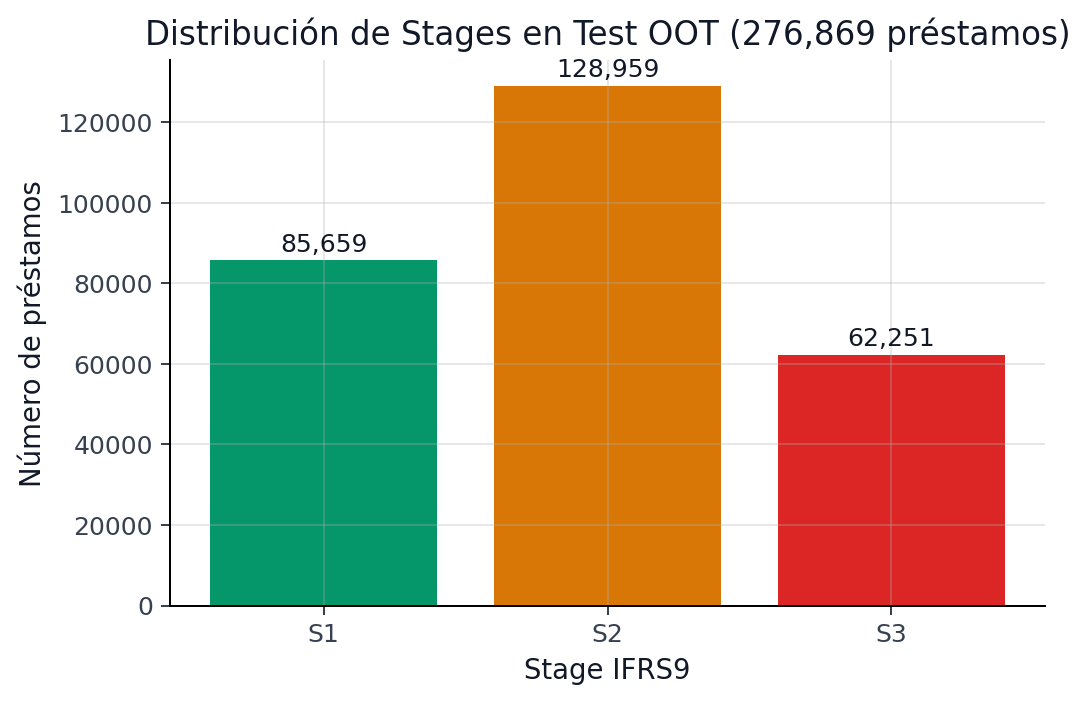
\includegraphics[keepaspectratio,alt={Gráfico de barras con la distribución de préstamos por Stage 1, Stage 2 y Stage 3 en el set de test IFRS9.}]{chapters/../assets/figures/notebooks/stage_distribution.png}}

}

\caption{\label{fig-stage-distribution}Distribución de préstamos por
stage IFRS9 en el set de test.}

\end{figure*}%

\begin{tcolorbox}[enhanced jigsaw, arc=.35mm, bottomrule=.15mm, bottomtitle=1mm, breakable, colback=white, colbacktitle=quarto-callout-note-color!10!white, colframe=quarto-callout-note-color-frame, coltitle=black, left=2mm, leftrule=.75mm, opacityback=0, opacitybacktitle=0.6, rightrule=.15mm, title=\textcolor{quarto-callout-note-color}{\faInfo}\hspace{0.5em}{¿Qué son los Stages IFRS9?}, titlerule=0mm, toprule=.15mm, toptitle=1mm]

\begin{itemize}
\tightlist
\item
  \textbf{Stage 1}: Préstamos sin deterioro significativo. Se
  provisionan con PD a 12 meses.
\item
  \textbf{Stage 2}: Préstamos con incremento significativo de riesgo
  crediticio (SICR). Se provisionan con PD de por vida.
\item
  \textbf{Stage 3}: Préstamos en default o credit-impaired. PD ≈ 1.0.
\end{itemize}

El 47\% del portafolio de test cae en Stage 2, reflejando que el período
2018--2020 incluye incrementos significativos de riesgo. Ver el capítulo
de IFRS9 para detalles.

\end{tcolorbox}

\section{Innovación central}\label{innovaciuxf3n-central}

La contribución principal del proyecto es el puente formal entre
\textbf{predicción conformal} y \textbf{optimización robusta}:

\begin{longtable}[]{@{}
  >{\raggedright\arraybackslash}p{(\linewidth - 4\tabcolsep) * \real{0.3158}}
  >{\raggedright\arraybackslash}p{(\linewidth - 4\tabcolsep) * \real{0.2368}}
  >{\raggedright\arraybackslash}p{(\linewidth - 4\tabcolsep) * \real{0.4474}}@{}}
\caption{Resumen de componentes del
pipeline}\label{tbl-innovation}\tabularnewline
\toprule\noalign{}
\begin{minipage}[b]{\linewidth}\raggedright
Componente
\end{minipage} & \begin{minipage}[b]{\linewidth}\raggedright
Técnica
\end{minipage} & \begin{minipage}[b]{\linewidth}\raggedright
Resultado clave
\end{minipage} \\
\midrule\noalign{}
\endfirsthead
\toprule\noalign{}
\begin{minipage}[b]{\linewidth}\raggedright
Componente
\end{minipage} & \begin{minipage}[b]{\linewidth}\raggedright
Técnica
\end{minipage} & \begin{minipage}[b]{\linewidth}\raggedright
Resultado clave
\end{minipage} \\
\midrule\noalign{}
\endhead
\bottomrule\noalign{}
\endlastfoot
Predicción & CatBoost calibrado con Venn-Abers & AUC 0.713, ECE 0.006 \\
Incertidumbre & Mondrian Conformal (MAPIE 1.3.0) & Cobertura 92.6\% @
90\% target \\
Decisión & Optimización robusta (Pyomo/HiGHS) & 299 préstamos, \$183K
retorno \\
Aprendizaje & SPO+ loss (PyEPO) & 49.1\% reducción de regret \\
Regulatorio & ECL bajo 4 escenarios & \$1.0B -- \$1.8B rango \\
Gobernanza & Fairness + MRM + Conformal Policy & 6/6 tests de equidad
pasados \\
\end{longtable}

\section{Linaje operativo congelado}\label{linaje-operativo-congelado}

\begin{longtable}[]{@{}
  >{\raggedright\arraybackslash}p{(\linewidth - 6\tabcolsep) * \real{0.2500}}
  >{\raggedright\arraybackslash}p{(\linewidth - 6\tabcolsep) * \real{0.2500}}
  >{\raggedright\arraybackslash}p{(\linewidth - 6\tabcolsep) * \real{0.2500}}
  >{\raggedright\arraybackslash}p{(\linewidth - 6\tabcolsep) * \real{0.2500}}@{}}
\caption{Linaje operativo de artefactos
congelados}\label{tbl-operational-lineage}\tabularnewline
\toprule\noalign{}
\begin{minipage}[b]{\linewidth}\raggedright
Capa
\end{minipage} & \begin{minipage}[b]{\linewidth}\raggedright
Artefactos clave
\end{minipage} & \begin{minipage}[b]{\linewidth}\raggedright
Productores
\end{minipage} & \begin{minipage}[b]{\linewidth}\raggedright
Consumidores
\end{minipage} \\
\midrule\noalign{}
\endfirsthead
\toprule\noalign{}
\begin{minipage}[b]{\linewidth}\raggedright
Capa
\end{minipage} & \begin{minipage}[b]{\linewidth}\raggedright
Artefactos clave
\end{minipage} & \begin{minipage}[b]{\linewidth}\raggedright
Productores
\end{minipage} & \begin{minipage}[b]{\linewidth}\raggedright
Consumidores
\end{minipage} \\
\midrule\noalign{}
\endhead
\bottomrule\noalign{}
\endlastfoot
Datos & \texttt{train.parquet}, \texttt{calibration.parquet},
\texttt{test.parquet} & \texttt{src/data/*} & PD, conformal, causal,
IFRS9 \\
Modelado & \texttt{pd\_canonical.cbm}, \texttt{model\_comparison.json} &
\texttt{scripts/train\_pd\_model.py} & conformal, explainability,
reporting \\
Incertidumbre & \texttt{conformal\_intervals\_mondrian.parquet},
\texttt{conformal\_policy\_status.json} &
\texttt{scripts/generate\_conformal\_intervals.py},
\texttt{scripts/validate\_conformal\_policy.py} & portfolio, IFRS9,
papers \\
Decisión & \texttt{portfolio\_allocations.parquet},
\texttt{champion\_portfolio\_policy.json} &
\texttt{scripts/optimize\_portfolio.py} & executive map, papers \\
Gobierno & \texttt{mrm\_validation\_report.json},
\texttt{fairness\_audit\_status.json} &
\texttt{scripts/generate\_mrm\_report.py},
\texttt{scripts/run\_fairness\_audit.py} & capítulo 10, agenda,
appendix \\
\end{longtable}

\section{Métricas de
investigación}\label{muxe9tricas-de-investigaciuxf3n}

\begin{table}

\caption{\label{tbl-research-metrics}Métricas clave para los papers de
investigación}

\centering{

\begin{Shaded}
\begin{Highlighting}[]
\NormalTok{causal }\OperatorTok{=}\NormalTok{ summary.get(}\StringTok{"causal"}\NormalTok{, \{\})}

\NormalTok{research }\OperatorTok{=}\NormalTok{ \{}
    \StringTok{"SPO+ regret reduction"}\NormalTok{: }\StringTok{"49.1\% vs two{-}stage"}\NormalTok{,}
    \StringTok{"BMA vs CP width"}\NormalTok{: }\StringTok{"CP 19.3\% más estrecho"}\NormalTok{,}
    \StringTok{"CIF lifetime PD correction"}\NormalTok{: }\StringTok{"KM sobreestima 26.7\%"}\NormalTok{,}
    \StringTok{"CIF exceso de reserva"}\NormalTok{: }\StringTok{"$125.8M"}\NormalTok{,}
    \StringTok{"SICR trigger óptimo"}\NormalTok{: }\StringTok{"t*=0.30, F1=0.2515"}\NormalTok{,}
    \StringTok{"ECL band (TS intervals)"}\NormalTok{: }\StringTok{"$288.5M (267}\SpecialCharTok{\% d}\StringTok{el punto)"}\NormalTok{,}
    \StringTok{"Stage cost óptimo"}\NormalTok{: }\StringTok{"pd\_thr=0.15, $97.3M"}\NormalTok{,}
    \StringTok{"ATE (int\_rate)"}\NormalTok{: }\SpecialStringTok{f"}\SpecialCharTok{\{}\NormalTok{causal}\SpecialCharTok{.}\NormalTok{get(}\StringTok{\textquotesingle{}ate\textquotesingle{}}\NormalTok{, }\DecValTok{0}\NormalTok{)}\SpecialCharTok{:.5f\}}\SpecialStringTok{"}\NormalTok{,}
    \StringTok{"CATE net value"}\NormalTok{: format\_money(causal.get(}\StringTok{"total\_net\_value"}\NormalTok{, }\DecValTok{0}\NormalTok{)),}
\NormalTok{\}}

\NormalTok{df\_research }\OperatorTok{=}\NormalTok{ pd.DataFrame(}\BuiltInTok{list}\NormalTok{(research.items()), columns}\OperatorTok{=}\NormalTok{[}\StringTok{"Métrica"}\NormalTok{, }\StringTok{"Valor"}\NormalTok{])}
\NormalTok{df\_research}
\end{Highlighting}
\end{Shaded}

}

\end{table}%

\section{Mapa de navegación}\label{mapa-de-navegaciuxf3n}

{\def\LTcaptype{none} % do not increment counter
\begin{longtable}[]{@{}
  >{\raggedright\arraybackslash}p{(\linewidth - 2\tabcolsep) * \real{0.5000}}
  >{\raggedright\arraybackslash}p{(\linewidth - 2\tabcolsep) * \real{0.5000}}@{}}
\toprule\noalign{}
\begin{minipage}[b]{\linewidth}\raggedright
Si te interesa\ldots{}
\end{minipage} & \begin{minipage}[b]{\linewidth}\raggedright
Ve a\ldots{}
\end{minipage} \\
\midrule\noalign{}
\endhead
\bottomrule\noalign{}
\endlastfoot
Cómo se construyó el modelo PD & Capítulo 6: Modelado de PD \\
Cómo funcionan los intervalos conformal & Capítulo 7: Predicción
Conformal \\
Cómo se optimiza el portafolio & Capítulo 9: Optimización de
Portafolio \\
Cómo se calculan las provisiones IFRS9 & Capítulo 10: IFRS9 y
Gobernanza \\
El paper de Predict-then-Optimize & Capítulo 14: Paper Estrella \\
El paper de IFRS9 End-to-End & Capítulo 15: Paper IFRS9 \\
El paper de Mondrian Conformal & Capítulo 16: Paper Mondrian \\
Benchmark GPU / RAPIDS & Apéndice B \\
\end{longtable}
}

\chapter{Glosario y Fundamentos}\label{glosario-y-fundamentos}

Este capítulo establece las bases conceptuales necesarias para entender
el resto del libro. Está dividido en cinco secciones, cada una cubriendo
una disciplina diferente que el proyecto integra. El objetivo es que un
lector con conocimiento básico o intermedio en cualquiera de estas áreas
pueda seguir la narrativa del pipeline y los papers de investigación.

No es necesario leer las cinco secciones antes de continuar --- se puede
usar como referencia y volver a consultar según la necesidad de cada
capítulo.

\chapter{Fundamentos de Riesgo
Crediticio}\label{sec-credit-risk-fundamentals}

\subsection{Probabilidad de Default
(PD)}\label{probabilidad-de-default-pd}

La \textbf{Probabilidad de Default} (PD) es la probabilidad estimada de
que un deudor no cumpla con sus obligaciones de pago dentro de un
horizonte de tiempo definido. En el marco de Basilea y IFRS9, la PD es
el primer componente del cálculo de pérdida esperada.

\begin{tcolorbox}[enhanced jigsaw, arc=.35mm, bottomrule=.15mm, bottomtitle=1mm, breakable, colback=white, colbacktitle=quarto-callout-note-color!10!white, colframe=quarto-callout-note-color-frame, coltitle=black, left=2mm, leftrule=.75mm, opacityback=0, opacitybacktitle=0.6, rightrule=.15mm, title=\textcolor{quarto-callout-note-color}{\faInfo}\hspace{0.5em}{PD a 12 meses vs PD de por vida}, titlerule=0mm, toprule=.15mm, toptitle=1mm]

\begin{itemize}
\tightlist
\item
  \textbf{PD a 12 meses (PD₁₂)}: Probabilidad de default dentro de los
  próximos 12 meses. Se usa para préstamos en Stage 1 bajo IFRS9.
\item
  \textbf{PD de por vida (PD\_lifetime)}: Probabilidad de default
  durante toda la vida restante del préstamo. Se usa para préstamos en
  Stage 2. Se estima típicamente con modelos de supervivencia (Cox PH,
  Random Survival Forest).
\end{itemize}

\end{tcolorbox}

En este proyecto, el modelo PD se entrena como un clasificador binario
(default/no-default) sobre datos de Lending Club resueltos. La salida es
una probabilidad continua en {[}0, 1{]} que se calibra para reflejar
frecuencias reales de default.

\subsection{Loss Given Default (LGD)}\label{loss-given-default-lgd}

La \textbf{Pérdida dado el Default} (LGD) mide la fracción del saldo
expuesto que no se recupera cuando un préstamo entra en default. Se
calcula como:

\begin{equation}\protect\phantomsection\label{eq-lgd}{
\text{LGD} = 1 - \text{Tasa de Recuperación} = 1 - \frac{\text{Monto Recuperado}}{\text{Exposición al Default}}
}\end{equation}

Valores típicos de LGD varían entre 20\% y 80\% según el tipo de
producto, la presencia de colateral y la efectividad de los procesos de
cobranza. En Lending Club, los préstamos son no garantizados, lo que
resulta en LGD relativamente altas.

\subsection{Exposure at Default (EAD)}\label{exposure-at-default-ead}

La \textbf{Exposición al Default} (EAD) es el monto total que el
prestamista tiene en riesgo en el momento del default. Para préstamos a
plazo fijo (como Lending Club), la EAD es el saldo pendiente del
principal más intereses acumulados. Para líneas de crédito revolventes,
la EAD incluye estimaciones de utilización futura (\emph{Credit
Conversion Factor}, CCF).

\subsection{Expected Credit Loss (ECL)}\label{expected-credit-loss-ecl}

La \textbf{Pérdida Crediticia Esperada} (ECL) es el producto de los tres
componentes anteriores, descontado al valor presente:

\begin{equation}\protect\phantomsection\label{eq-ecl}{
\text{ECL} = \text{PD} \times \text{LGD} \times \text{EAD} \times \text{Factor de Descuento}
}\end{equation}

Este es el cálculo central de IFRS9 y determina las provisiones que un
banco debe reservar para cubrir pérdidas anticipadas.

\subsection{IFRS9 y el Modelo de Tres
Stages}\label{ifrs9-y-el-modelo-de-tres-stages}

IFRS9 (International Financial Reporting Standard 9) es la norma
contable internacional que rige la clasificación y medición de
instrumentos financieros. Su modelo de deterioro se basa en tres stages:

\begin{longtable}[]{@{}
  >{\raggedright\arraybackslash}p{(\linewidth - 6\tabcolsep) * \real{0.1667}}
  >{\raggedright\arraybackslash}p{(\linewidth - 6\tabcolsep) * \real{0.2619}}
  >{\raggedright\arraybackslash}p{(\linewidth - 6\tabcolsep) * \real{0.3095}}
  >{\raggedright\arraybackslash}p{(\linewidth - 6\tabcolsep) * \real{0.2619}}@{}}
\caption{Modelo de deterioro de tres stages de
IFRS9}\label{tbl-ifrs9-stages}\tabularnewline
\toprule\noalign{}
\begin{minipage}[b]{\linewidth}\raggedright
Stage
\end{minipage} & \begin{minipage}[b]{\linewidth}\raggedright
Condición
\end{minipage} & \begin{minipage}[b]{\linewidth}\raggedright
PD Utilizada
\end{minipage} & \begin{minipage}[b]{\linewidth}\raggedright
Provisión
\end{minipage} \\
\midrule\noalign{}
\endfirsthead
\toprule\noalign{}
\begin{minipage}[b]{\linewidth}\raggedright
Stage
\end{minipage} & \begin{minipage}[b]{\linewidth}\raggedright
Condición
\end{minipage} & \begin{minipage}[b]{\linewidth}\raggedright
PD Utilizada
\end{minipage} & \begin{minipage}[b]{\linewidth}\raggedright
Provisión
\end{minipage} \\
\midrule\noalign{}
\endhead
\bottomrule\noalign{}
\endlastfoot
\textbf{Stage 1} & Sin deterioro significativo & PD a 12 meses & ECL a
12 meses \\
\textbf{Stage 2} & Incremento significativo de riesgo (SICR) & PD de por
vida & ECL de por vida \\
\textbf{Stage 3} & Default confirmado (≥90 DPD) & PD ≈ 1.0 & ECL
total \\
\end{longtable}

\subsection{Incremento Significativo de Riesgo Crediticio
(SICR)}\label{incremento-significativo-de-riesgo-crediticio-sicr}

El \textbf{SICR} (Significant Increase in Credit Risk) es el trigger que
mueve un préstamo de Stage 1 a Stage 2. IFRS9 no prescribe un método
único para detectarlo --- cada institución define sus propios criterios.
Criterios comunes incluyen:

\begin{itemize}
\tightlist
\item
  Incremento absoluto o relativo de PD respecto a la originación
\item
  Días de mora (30+ DPD como backstop)
\item
  Downgrade de calificación interna
\end{itemize}

\begin{tcolorbox}[enhanced jigsaw, arc=.35mm, bottomrule=.15mm, bottomtitle=1mm, breakable, colback=white, colbacktitle=quarto-callout-tip-color!10!white, colframe=quarto-callout-tip-color-frame, coltitle=black, left=2mm, leftrule=.75mm, opacityback=0, opacitybacktitle=0.6, rightrule=.15mm, title=\textcolor{quarto-callout-tip-color}{\faLightbulb}\hspace{0.5em}{Innovación del proyecto}, titlerule=0mm, toprule=.15mm, toptitle=1mm]

En este proyecto proponemos usar el \textbf{ancho del intervalo
conformal} como señal adicional de SICR. Un intervalo más ancho indica
mayor incertidumbre sobre la PD, lo que puede señalar deterioro antes de
que se refleje en el punto estimado. Esta es una contribución original
--- no existen papers previos que usen el ancho conformal como trigger
SICR.

\end{tcolorbox}

\subsection{Basilea III y Capital
Regulatorio}\label{basilea-iii-y-capital-regulatorio}

El \textbf{marco de Basilea III} establece requerimientos mínimos de
capital que los bancos deben mantener para absorber pérdidas
inesperadas. Los tres pilares relevantes son:

\begin{enumerate}
\def\labelenumi{\arabic{enumi}.}
\tightlist
\item
  \textbf{Pilar 1 --- Capital mínimo}: Fórmulas regulatorias basadas en
  PD, LGD y EAD para calcular activos ponderados por riesgo (RWA).
\item
  \textbf{Pilar 2 --- Supervisión}: Evaluaciones internas de adecuación
  de capital (ICAAP), incluyendo tests de estrés.
\item
  \textbf{Pilar 3 --- Transparencia}: Divulgación pública de métricas de
  riesgo y modelos utilizados.
\end{enumerate}

\subsection{Grados de Riesgo (Credit
Grades)}\label{grados-de-riesgo-credit-grades}

En Lending Club, los préstamos se clasifican en grados de A (menor
riesgo) a G (mayor riesgo), basados en la evaluación crediticia del
solicitante al momento de la originación. Estos grados determinan la
tasa de interés y se utilizan en este proyecto como \textbf{variable de
partición Mondrian} para predicción conformal condicional.

\begin{longtable}[]{@{}lll@{}}
\caption{Grados de riesgo de Lending Club (valores aproximados del
dataset)}\label{tbl-credit-grades}\tabularnewline
\toprule\noalign{}
Grado & Tasa de Default Típica & Tasa de Interés Típica \\
\midrule\noalign{}
\endfirsthead
\toprule\noalign{}
Grado & Tasa de Default Típica & Tasa de Interés Típica \\
\midrule\noalign{}
\endhead
\bottomrule\noalign{}
\endlastfoot
A & \textasciitilde5--8\% & \textasciitilde6--8\% \\
B & \textasciitilde10--14\% & \textasciitilde10--12\% \\
C & \textasciitilde15--20\% & \textasciitilde13--16\% \\
D & \textasciitilde20--28\% & \textasciitilde17--21\% \\
E & \textasciitilde28--35\% & \textasciitilde22--26\% \\
F & \textasciitilde35--45\% & \textasciitilde26--30\% \\
G & \textasciitilde45--55\% & \textasciitilde30--31\% \\
\end{longtable}

\chapter{Fundamentos de ML y Estadística}\label{sec-ml-foundations}

\subsection{Métricas de
Discriminación}\label{muxe9tricas-de-discriminaciuxf3n}

Las métricas de discriminación evalúan qué tan bien un modelo separa
defaults de no-defaults.

\textbf{AUC-ROC} (Area Under the Receiver Operating Characteristic
Curve): Mide la probabilidad de que el modelo asigne un score más alto a
un default positivo seleccionado al azar que a un negativo seleccionado
al azar. Rango: 0.5 (aleatorio) a 1.0 (perfecto). En credit scoring, AUC
\textgreater{} 0.70 se considera aceptable para producción.

\textbf{Gini}: Transformación lineal del AUC:
\(\text{Gini} = 2 \times \text{AUC} - 1\). Rango: 0 (aleatorio) a 1
(perfecto). Es la métrica más utilizada en la industria bancaria
europea.

\textbf{KS (Kolmogorov-Smirnov)}: Máxima distancia vertical entre las
distribuciones acumuladas de los scores de defaults y no-defaults.
Indica el punto de máxima separación entre las dos poblaciones.

\textbf{PR-AUC} (Area Under the Precision-Recall Curve): Especialmente
relevante para datasets desbalanceados. En Lending Club, con
\textasciitilde20\% de default rate, PR-AUC complementa al AUC-ROC
capturando el rendimiento sobre la clase minoritaria (o mayoritaria en
riesgo).

\subsection{Métricas de
Calibración}\label{muxe9tricas-de-calibraciuxf3n}

La calibración mide si las probabilidades predichas reflejan las
frecuencias reales de default. Un modelo puede tener excelente
discriminación (AUC alto) pero mala calibración.

\textbf{Brier Score}: Error cuadrático medio entre las probabilidades
predichas y los outcomes binarios:

\begin{equation}\protect\phantomsection\label{eq-brier}{
\text{Brier} = \frac{1}{n} \sum_{i=1}^{n} (\hat{p}_i - y_i)^2
}\end{equation}

Rango: 0 (perfecto) a 1 (peor caso). Para un dataset con 20\% default
rate, un modelo naive que predice 0.20 para todos obtiene Brier ≈ 0.16.

\textbf{ECE} (Expected Calibration Error): Promedio ponderado de la
diferencia absoluta entre la confianza predicha y la precisión
observada, calculada por bins:

\begin{equation}\protect\phantomsection\label{eq-ece}{
\text{ECE} = \sum_{b=1}^{B} \frac{|B_b|}{n} \left| \text{acc}(B_b) - \text{conf}(B_b) \right|
}\end{equation}

Un ECE \textless{} 0.01 indica calibración excelente. Nuestro modelo
calibrado con Venn-Abers logra ECE = 0.006.

\textbf{D² Brier}: Análogo al R² para el Brier Score, mide la mejora
relativa del modelo sobre un predictor naive (frecuencia marginal).

\subsection{Gradient Boosting y
CatBoost}\label{gradient-boosting-y-catboost}

\textbf{Gradient Boosting} es un ensemble de árboles de decisión
entrenados secuencialmente, donde cada árbol corrige los errores del
anterior. La predicción final es la suma ponderada de todas las
predicciones individuales.

\textbf{CatBoost} (Categorical Boosting) es una implementación de
gradient boosting desarrollada por Yandex con tres ventajas clave para
credit scoring:

\begin{enumerate}
\def\labelenumi{\arabic{enumi}.}
\tightlist
\item
  \textbf{Manejo nativo de categorías}: No requiere one-hot encoding ni
  WOE manual para variables categóricas --- aplica target encoding con
  regularización ordered boosting.
\item
  \textbf{Manejo nativo de valores faltantes}: Trata NaN como un valor
  informativo, asignándolo a la rama óptima de cada split.
\item
  \textbf{Ordered boosting}: Reduce el overfitting al usar subconjuntos
  de datos históricos para calcular los target statistics de cada
  observación.
\end{enumerate}

\begin{tcolorbox}[enhanced jigsaw, arc=.35mm, bottomrule=.15mm, bottomtitle=1mm, breakable, colback=white, colbacktitle=quarto-callout-note-color!10!white, colframe=quarto-callout-note-color-frame, coltitle=black, left=2mm, leftrule=.75mm, opacityback=0, opacitybacktitle=0.6, rightrule=.15mm, title=\textcolor{quarto-callout-note-color}{\faInfo}\hspace{0.5em}{¿Por qué CatBoost y no XGBoost o LightGBM?}, titlerule=0mm, toprule=.15mm, toptitle=1mm]

En credit scoring con datos tabulares, CatBoost ofrece: (1) mejor
calibración out-of-the-box gracias al ordered boosting, (2) manejo
transparente de categorías sin preprocesamiento manual, y (3) menor
sensibilidad a hiperparámetros. Estudios comparativos recientes en
credit scoring (Ayari et~al., 2026; {Lessmann et~al.}, 2015) confirman
que los tres frameworks logran AUC comparable, pero CatBoost simplifica
el pipeline de features y reduce el riesgo de data leakage por target
encoding incorrecto.

\end{tcolorbox}

\subsection{Optimización de Hiperparámetros
(HPO)}\label{optimizaciuxf3n-de-hiperparuxe1metros-hpo}

\textbf{Optuna} es un framework de optimización de hiperparámetros
basado en Tree-structured Parzen Estimator (TPE). A diferencia de grid
search o random search, TPE modela la distribución de hiperparámetros
condicional a su rendimiento y muestrea nuevos candidatos de las
regiones más prometedoras.

En este proyecto, Optuna ejecuta 320 trials para el espacio de CatBoost,
optimizando profundidad, learning rate, regularización L2, bagging
temperature y otros hiperparámetros. La métrica objetivo es AUC validado
sobre el split temporal de validación.

\subsection{Calibración de
Probabilidades}\label{calibraciuxf3n-de-probabilidades}

Un modelo de clasificación produce scores que no necesariamente son
probabilidades bien calibradas. Los métodos de calibración post-hoc
transforman los scores en probabilidades:

\begin{itemize}
\tightlist
\item
  \textbf{Platt Scaling}: Ajusta una regresión logística sobre los
  scores del modelo para producir probabilidades calibradas. Supone una
  relación sigmoide entre score y probabilidad.
\item
  \textbf{Isotonic Regression}: Ajuste no paramétrico monótono. Más
  flexible que Platt pero propenso a overfitting con pocas muestras.
\item
  \textbf{Venn-Abers}: Produce intervalos de probabilidad con garantías
  de validez multiprobabilística. Es el método más conservador y el
  seleccionado en este proyecto por su robustez temporal.
\end{itemize}

\subsection{Weight of Evidence (WOE) e Information Value
(IV)}\label{weight-of-evidence-woe-e-information-value-iv}

\textbf{WOE} (Weight of Evidence) transforma variables categóricas o
numéricas binneadas en una escala que refleja su poder predictivo:

\begin{equation}\protect\phantomsection\label{eq-woe}{
\text{WOE}_i = \ln \left( \frac{\% \text{ no-defaults en bin } i}{\% \text{ defaults en bin } i} \right)
}\end{equation}

\textbf{IV} (Information Value) mide el poder predictivo total de una
variable:

\begin{equation}\protect\phantomsection\label{eq-iv}{
\text{IV} = \sum_{i=1}^{k} (\% \text{ no-defaults}_i - \% \text{ defaults}_i) \times \text{WOE}_i
}\end{equation}

\begin{longtable}[]{@{}ll@{}}
\caption{Interpretación del Information
Value}\label{tbl-iv-interpretation}\tabularnewline
\toprule\noalign{}
IV & Poder predictivo \\
\midrule\noalign{}
\endfirsthead
\toprule\noalign{}
IV & Poder predictivo \\
\midrule\noalign{}
\endhead
\bottomrule\noalign{}
\endlastfoot
\textless{} 0.02 & No útil \\
0.02 -- 0.10 & Débil \\
0.10 -- 0.30 & Medio \\
0.30 -- 0.50 & Fuerte \\
\textgreater{} 0.50 & Sospechosamente fuerte (posible leakage) \\
\end{longtable}

\chapter{Incertidumbre y Predicción
Conformal}\label{sec-uncertainty-conformal}

La cuantificación de incertidumbre es una de las piezas más críticas ---
y frecuentemente ignoradas --- en la modelación de riesgo crediticio. Un
modelo que produce una estimación puntual de \(\hat{p} = 0.15\) para la
probabilidad de default de un préstamo no transmite si esa estimación es
confiable o altamente incierta. En un portafolio de miles de préstamos,
tomar decisiones de asignación basadas exclusivamente en puntos
estimados sin considerar su incertidumbre conduce a portafolios frágiles
que se deterioran bajo condiciones adversas.

Esta sección introduce los fundamentos teóricos de la cuantificación de
incertidumbre, con énfasis particular en la \textbf{predicción
conformal} --- un marco que ofrece garantías matemáticas de cobertura
sin requerir supuestos distribucionales sobre los datos.

\subsection{Incertidumbre Aleatórica vs
Epistémica}\label{sec-aleatoric-epistemic}

La incertidumbre en las predicciones de un modelo tiene dos fuentes
fundamentalmente distintas:

\textbf{Incertidumbre aleatórica} (irreducible): Es la variabilidad
inherente al fenómeno observado. Proviene de la estocasticidad
intrínseca del proceso generador de datos y no puede eliminarse
recopilando más datos ni mejorando el modelo. En riesgo crediticio, la
incertidumbre aleatórica refleja que dos prestatarios con exactamente
las mismas características observables pueden tener outcomes distintos:
uno paga y el otro entra en default. Esto ocurre porque existen factores
no observados --- eventos de salud, pérdida de empleo, decisiones
personales --- que afectan el repago pero no están capturados en las
features del modelo.

\textbf{Incertidumbre epistémica} (reducible): Es la incertidumbre que
surge de la limitación del conocimiento del modelo. Se debe a datos
insuficientes, especificación incorrecta del modelo, o regiones del
espacio de features con poca representación en el conjunto de
entrenamiento. A diferencia de la aleatórica, esta incertidumbre
\emph{puede} reducirse con más datos o un modelo mejor especificado.

\begin{tcolorbox}[enhanced jigsaw, arc=.35mm, bottomrule=.15mm, bottomtitle=1mm, breakable, colback=white, colbacktitle=quarto-callout-note-color!10!white, colframe=quarto-callout-note-color-frame, coltitle=black, left=2mm, leftrule=.75mm, opacityback=0, opacitybacktitle=0.6, rightrule=.15mm, title=\textcolor{quarto-callout-note-color}{\faInfo}\hspace{0.5em}{Ejemplo en riesgo crediticio}, titlerule=0mm, toprule=.15mm, toptitle=1mm]

Considérese un préstamo de grado G con un historial crediticio muy
corto. La incertidumbre sobre su PD tiene ambos componentes:

\begin{itemize}
\tightlist
\item
  \textbf{Aleatórica}: Aun conociendo perfectamente todas las
  características del prestatario, existe variabilidad inherente en si
  entrará o no en default.
\item
  \textbf{Epistémica}: Dado que los préstamos grado G con historial
  corto son relativamente escasos en el conjunto de entrenamiento, el
  modelo tiene menos evidencia para estimar su PD con precisión. Con más
  datos de prestatarios similares, esta componente se reduciría.
\end{itemize}

En la práctica, los intervalos conformales capturan ambas fuentes de
incertidumbre simultáneamente, sin necesidad de descomponerlas
explícitamente.

\end{tcolorbox}

En la modelación Bayesiana, la incertidumbre epistémica se captura a
través de la distribución posterior sobre los parámetros del modelo,
mientras que la aleatórica se captura a través de la distribución
predictiva posterior. Los métodos conformales, en cambio, producen
intervalos que absorben ambas fuentes de forma agnóstica --- no
requieren especificar un prior ni una verosimilitud, lo que los hace
especialmente atractivos para aplicaciones regulatorias donde la
transparencia y la ausencia de supuestos son valoradas.

\subsection{Intervalos de Predicción vs Intervalos de
Confianza}\label{sec-prediction-vs-confidence}

Una confusión frecuente en la práctica estadística --- y particularmente
peligrosa en gestión de riesgo --- es la diferencia entre intervalos de
confianza e intervalos de predicción. Aunque ambos producen rangos
numéricos, cuantifican objetos fundamentalmente distintos.

\textbf{Intervalo de confianza} para un parámetro \(\theta\) al nivel
\(1 - \alpha\): Es un rango \([\hat{\theta}_L, \hat{\theta}_U]\) tal
que, bajo muestreo repetido:

\begin{equation}\protect\phantomsection\label{eq-confidence-interval}{
P\left(\theta \in [\hat{\theta}_L, \hat{\theta}_U]\right) \geq 1 - \alpha
}\end{equation}

El intervalo de confianza cuantifica la incertidumbre sobre un
\emph{parámetro poblacional} (por ejemplo, la tasa de default promedio
de un segmento). Se estrecha con más datos porque la estimación del
parámetro mejora.

\textbf{Intervalo de predicción} para una nueva observación \(Y_{n+1}\)
al nivel \(1 - \alpha\): Es un rango \([L(X_{n+1}), U(X_{n+1})]\) tal
que:

\begin{equation}\protect\phantomsection\label{eq-prediction-interval}{
P\left(Y_{n+1} \in [L(X_{n+1}), U(X_{n+1})]\right) \geq 1 - \alpha
}\end{equation}

El intervalo de predicción cuantifica la incertidumbre sobre una
\emph{observación futura individual}. Incluye tanto la incertidumbre
sobre el parámetro (epistémica) como la variabilidad inherente del
outcome (aleatórica), por lo que es necesariamente más ancho que el
intervalo de confianza correspondiente.

\begin{longtable}[]{@{}
  >{\raggedright\arraybackslash}p{(\linewidth - 4\tabcolsep) * \real{0.1930}}
  >{\raggedright\arraybackslash}p{(\linewidth - 4\tabcolsep) * \real{0.3860}}
  >{\raggedright\arraybackslash}p{(\linewidth - 4\tabcolsep) * \real{0.4211}}@{}}
\caption{Comparación entre intervalos de confianza e intervalos de
predicción}\label{tbl-ci-vs-pi}\tabularnewline
\toprule\noalign{}
\begin{minipage}[b]{\linewidth}\raggedright
Propiedad
\end{minipage} & \begin{minipage}[b]{\linewidth}\raggedright
Intervalo de Confianza
\end{minipage} & \begin{minipage}[b]{\linewidth}\raggedright
Intervalo de Predicción
\end{minipage} \\
\midrule\noalign{}
\endfirsthead
\toprule\noalign{}
\begin{minipage}[b]{\linewidth}\raggedright
Propiedad
\end{minipage} & \begin{minipage}[b]{\linewidth}\raggedright
Intervalo de Confianza
\end{minipage} & \begin{minipage}[b]{\linewidth}\raggedright
Intervalo de Predicción
\end{minipage} \\
\midrule\noalign{}
\endhead
\bottomrule\noalign{}
\endlastfoot
\textbf{Objeto cuantificado} & Parámetro poblacional \(\theta\) &
Observación futura \(Y_{n+1}\) \\
\textbf{Fuentes de incertidumbre} & Solo epistémica & Epistémica +
aleatórica \\
\textbf{Comportamiento con \(n \to \infty\)} & Se estrecha a cero &
Converge a un ancho mínimo \textgreater{} 0 \\
\textbf{Uso en riesgo crediticio} & Tasa de default de un segmento & PD
de un préstamo individual \\
\textbf{Error común} & Usar como si fuera predicción & Ignorar la
componente aleatórica \\
\end{longtable}

\begin{tcolorbox}[enhanced jigsaw, arc=.35mm, bottomrule=.15mm, bottomtitle=1mm, breakable, colback=white, colbacktitle=quarto-callout-warning-color!10!white, colframe=quarto-callout-warning-color-frame, coltitle=black, left=2mm, leftrule=.75mm, opacityback=0, opacitybacktitle=0.6, rightrule=.15mm, title=\textcolor{quarto-callout-warning-color}{\faExclamationTriangle}\hspace{0.5em}{Error frecuente en la práctica bancaria}, titlerule=0mm, toprule=.15mm, toptitle=1mm]

En muchos modelos de riesgo crediticio en producción, se reportan
intervalos de confianza sobre la PD media de un segmento como si fueran
intervalos de predicción para préstamos individuales. Esto subestima
sistemáticamente la incertidumbre: un intervalo de confianza al 95\%
para la PD media de grado B podría ser {[}0.11, 0.13{]}, mientras que el
intervalo de predicción individual correcto podría ser {[}0.02, 0.35{]}.
La diferencia es crucial para la gestión de portafolio y la
determinación de provisiones bajo IFRS9.

\end{tcolorbox}

En este proyecto, todos los intervalos generados son \textbf{intervalos
de predicción} --- cuantifican la incertidumbre sobre la PD de cada
préstamo individual, no sobre parámetros promedio de segmentos.

\subsection{Fundamentos de la Predicción
Conformal}\label{sec-conformal-fundamentals}

La predicción conformal, introducida por Vovk, Gammerman y Shafer (Vovk
et~al., 2005), es un marco teórico para construir intervalos de
predicción con \textbf{garantías finitas de cobertura} sin asumir una
distribución paramétrica específica para los datos. Esta propiedad la
distingue fundamentalmente de los intervalos paramétricos (que requieren
supuestos distribucionales) y los intervalos bootstrap (que son
asintóticos y pueden fallar en muestras finitas).

\subsubsection{El supuesto de
intercambiabilidad}\label{sec-exchangeability}

El único supuesto teórico requerido por la predicción conformal es la
\textbf{intercambiabilidad} (\emph{exchangeability}) de los datos. Una
secuencia de variables aleatorias \((Z_1, Z_2, \ldots, Z_n)\) es
intercambiable si su distribución conjunta es invariante bajo cualquier
permutación:

\begin{equation}\protect\phantomsection\label{eq-exchangeability}{
P(Z_1, Z_2, \ldots, Z_n) = P(Z_{\pi(1)}, Z_{\pi(2)}, \ldots, Z_{\pi(n)}) \quad \forall \pi \in S_n
}\end{equation}

donde \(S_n\) es el grupo de todas las permutaciones de
\(\{1, 2, \ldots, n\}\).

La intercambiabilidad es estrictamente más débil que el supuesto i.i.d.
(independiente e idénticamente distribuido): todas las secuencias i.i.d.
son intercambiables, pero no toda secuencia intercambiable es i.i.d. Por
ejemplo, un muestreo sin reemplazo de una urna finita produce secuencias
intercambiables pero no independientes.

\begin{tcolorbox}[enhanced jigsaw, arc=.35mm, bottomrule=.15mm, bottomtitle=1mm, breakable, colback=white, colbacktitle=quarto-callout-tip-color!10!white, colframe=quarto-callout-tip-color-frame, coltitle=black, left=2mm, leftrule=.75mm, opacityback=0, opacitybacktitle=0.6, rightrule=.15mm, title=\textcolor{quarto-callout-tip-color}{\faLightbulb}\hspace{0.5em}{Intercambiabilidad en datos de crédito}, titlerule=0mm, toprule=.15mm, toptitle=1mm]

En este proyecto, los splits temporales (train/calibración/test) violan
la intercambiabilidad estricta porque la distribución de préstamos puede
cambiar con el tiempo (concept drift). Sin embargo, la predicción
conformal es notablemente robusta en la práctica: incluso bajo
desviaciones moderadas de la intercambiabilidad, la cobertura empírica
permanece cercana a la garantía teórica. En nuestros experimentos con
datos OOT (2018--2020), la cobertura empírica al 90\% alcanza 92.52\%
--- ligeramente por encima de la garantía, lo que indica conservadurismo
saludable.

\end{tcolorbox}

\subsubsection{La garantía de cobertura}\label{sec-coverage-guarantee}

El resultado central de la predicción conformal es el siguiente teorema:

\begin{tcolorbox}[enhanced jigsaw, arc=.35mm, bottomrule=.15mm, bottomtitle=1mm, breakable, colback=white, colbacktitle=quarto-callout-note-color!10!white, colframe=quarto-callout-note-color-frame, coltitle=black, left=2mm, leftrule=.75mm, opacityback=0, opacitybacktitle=0.6, rightrule=.15mm, title=\textcolor{quarto-callout-note-color}{\faInfo}\hspace{0.5em}{Teorema de cobertura conformal}, titlerule=0mm, toprule=.15mm, toptitle=1mm]

Sean \((X_1, Y_1), \ldots, (X_n, Y_n), (X_{n+1}, Y_{n+1})\) variables
aleatorias intercambiables. Para cualquier función de nonconformidad
\(s\) y cualquier nivel de significancia \(\alpha \in (0, 1)\), el
conjunto de predicción conformal \(C_\alpha(X_{n+1})\) satisface:

\begin{equation}\protect\phantomsection\label{eq-coverage-guarantee}{
P\left(Y_{n+1} \in C_\alpha(X_{n+1})\right) \geq 1 - \alpha
}\end{equation}

Más precisamente, bajo intercambiabilidad:

\begin{equation}\protect\phantomsection\label{eq-coverage-exact}{
1 - \alpha \leq P\left(Y_{n+1} \in C_\alpha(X_{n+1})\right) \leq 1 - \alpha + \frac{1}{n+1}
}\end{equation}

donde \(n\) es el tamaño del conjunto de calibración.

\end{tcolorbox}

La Ecuación~\ref{eq-coverage-exact} muestra que la cobertura es
\emph{exacta} hasta un factor \(\frac{1}{n+1}\) que se vuelve
despreciable para conjuntos de calibración grandes. Para
\(n = 237{,}584\) (el tamaño de nuestro conjunto de calibración),
\(\frac{1}{n+1} \approx 4.2 \times 10^{-6}\), haciendo la garantía
prácticamente exacta.

Esta garantía es \textbf{marginal} --- se cumple en promedio sobre la
distribución conjunta de los datos de calibración y el nuevo punto de
test. No garantiza cobertura condicional para cada subgrupo de préstamos
(para eso se necesita el enfoque Mondrian, descrito en
Sección~\ref{sec-mondrian-primer}).

\subsubsection{Scores de
nonconformidad}\label{sec-nonconformity-scores-primer}

El concepto central del framework conformal es el \textbf{score de
nonconformidad} (\emph{nonconformity score}), denotado \(s(x, y)\). Este
score mide qué tan ``inusual'' o ``no conforme'' es una observación
\((x, y)\) respecto al patrón aprendido por el modelo. A mayor score,
más atípica es la observación.

Para regresión (y para la estimación de intervalos de PD), el score más
común es el \textbf{residuo absoluto}:

\begin{equation}\protect\phantomsection\label{eq-residual-score}{
s_i = |y_i - \hat{f}(x_i)|
}\end{equation}

donde \(\hat{f}(x_i)\) es la predicción del modelo para la observación
\(i\). En nuestro caso, \(\hat{f}(x_i)\) es la PD calibrada y
\(y_i \in \{0, 1\}\) es el indicador binario de default.

Otros scores de nonconformidad incluyen:

\begin{itemize}
\tightlist
\item
  \textbf{Residuo escalado}:
  \(s_i = \frac{|y_i - \hat{f}(x_i)|}{\hat{\sigma}(x_i)}\), donde
  \(\hat{\sigma}(x_i)\) es una estimación local de dispersión. Produce
  intervalos de ancho variable (\emph{heteroscedásticos}).
\item
  \textbf{Residuo normalizado}:
  \(s_i = \frac{|y_i - \hat{f}(x_i)|}{\sqrt{\hat{f}(x_i)(1 - \hat{f}(x_i))}}\),
  que normaliza por la varianza binomial. En nuestro código, esto
  corresponde al parámetro \texttt{scaled\_scores=True}.
\item
  \textbf{Score CQR}: Basado en cuantiles condicionales (ver
  Sección~\ref{sec-cqr}).
\end{itemize}

La elección del score afecta la \emph{eficiencia} (ancho de los
intervalos) pero no la \emph{validez} (garantía de cobertura). Cualquier
función de score produce intervalos con cobertura válida; scores más
sofisticados producen intervalos más estrechos.

\subsection{Split Conformal}\label{sec-split-conformal-primer}

El \textbf{Split Conformal} (o \emph{Inductive Conformal Prediction}) es
la variante más práctica y computacionalmente eficiente de la predicción
conformal. Su implementación requiere tres pasos simples.

\subsubsection{Procedimiento formal}\label{sec-split-procedure}

Dados un modelo \(\hat{f}\) ya entrenado, un conjunto de calibración
\(\mathcal{D}_\text{cal} = \{(X_i, Y_i)\}_{i=1}^{n}\) \textbf{no
utilizado durante el entrenamiento}, y un nivel de cobertura deseado
\(1 - \alpha\):

\textbf{Paso 1 --- Calcular scores de nonconformidad en calibración:}

\begin{equation}\protect\phantomsection\label{eq-split-step1}{
s_i = |Y_i - \hat{f}(X_i)|, \quad i = 1, \ldots, n
}\end{equation}

\textbf{Paso 2 --- Calcular el cuantil conformal:}

\begin{equation}\protect\phantomsection\label{eq-split-quantile}{
\hat{q}_\alpha = \text{Quantile}\left(\{s_1, \ldots, s_n\}, \frac{\lceil (n+1)(1-\alpha) \rceil}{n}\right)
}\end{equation}

El nivel del cuantil incorpora la corrección de muestra finita
\(\frac{\lceil (n+1)(1-\alpha) \rceil}{n}\) que garantiza la cobertura
exacta de la Ecuación~\ref{eq-coverage-exact}.

\textbf{Paso 3 --- Construir intervalos para nuevas observaciones:}

\begin{equation}\protect\phantomsection\label{eq-split-interval}{
C_\alpha(X_{n+1}) = \left[\hat{f}(X_{n+1}) - \hat{q}_\alpha, \; \hat{f}(X_{n+1}) + \hat{q}_\alpha\right]
}\end{equation}

Para PD, los intervalos se truncan a \([0, 1]\):
\(C_\alpha(X_{n+1}) \cap [0, 1]\).

\begin{tcolorbox}[enhanced jigsaw, arc=.35mm, bottomrule=.15mm, bottomtitle=1mm, breakable, colback=white, colbacktitle=quarto-callout-tip-color!10!white, colframe=quarto-callout-tip-color-frame, coltitle=black, left=2mm, leftrule=.75mm, opacityback=0, opacitybacktitle=0.6, rightrule=.15mm, title=\textcolor{quarto-callout-tip-color}{\faLightbulb}\hspace{0.5em}{Elegancia computacional}, titlerule=0mm, toprule=.15mm, toptitle=1mm]

Nótese que el procedimiento Split Conformal requiere una sola pasada de
predicción sobre el conjunto de calibración y el cálculo de un único
cuantil. No hay refitting del modelo, no hay bootstrapping, no hay
simulación Monte Carlo. Esto hace que sea extremadamente eficiente
computacionalmente --- en nuestro pipeline, generar intervalos
conformales para 276,869 préstamos de test toma menos de un segundo una
vez que el modelo está entrenado.

\end{tcolorbox}

\subsubsection{Requisito del conjunto de calibración
separado}\label{sec-calibration-holdout}

Un aspecto fundamental del Split Conformal es que el conjunto de
calibración debe ser \textbf{estrictamente independiente} del conjunto
de entrenamiento. Si se usan los mismos datos para entrenar el modelo y
para calcular los scores de nonconformidad, los scores serán
optimistamente pequeños (el modelo se ajusta bien a sus propios datos de
entrenamiento) y los intervalos resultantes serán demasiado estrechos,
violando la garantía de cobertura.

En nuestro proyecto, la separación se garantiza mediante splits
temporales:

\begin{longtable}[]{@{}
  >{\raggedright\arraybackslash}p{(\linewidth - 4\tabcolsep) * \real{0.4167}}
  >{\raggedright\arraybackslash}p{(\linewidth - 4\tabcolsep) * \real{0.3750}}
  >{\raggedright\arraybackslash}p{(\linewidth - 4\tabcolsep) * \real{0.2083}}@{}}
\caption{Splits temporales del proyecto y su rol en el framework
conformal}\label{tbl-temporal-splits}\tabularnewline
\toprule\noalign{}
\begin{minipage}[b]{\linewidth}\raggedright
Conjunto
\end{minipage} & \begin{minipage}[b]{\linewidth}\raggedright
Período
\end{minipage} & \begin{minipage}[b]{\linewidth}\raggedright
Uso
\end{minipage} \\
\midrule\noalign{}
\endfirsthead
\toprule\noalign{}
\begin{minipage}[b]{\linewidth}\raggedright
Conjunto
\end{minipage} & \begin{minipage}[b]{\linewidth}\raggedright
Período
\end{minipage} & \begin{minipage}[b]{\linewidth}\raggedright
Uso
\end{minipage} \\
\midrule\noalign{}
\endhead
\bottomrule\noalign{}
\endlastfoot
Train & 2007-06 a 2017-03 & Entrenamiento del modelo CatBoost \\
Calibración & 2017-03 a 2017-12 & Cálculo de scores conformales
(\(n = 237{,}584\)) \\
Test (OOT) & 2018-01 a 2020-09 & Evaluación de cobertura
(\(n = 276{,}869\)) \\
\end{longtable}

\subsubsection{Implementación con MAPIE 1.3.0}\label{sec-mapie-api}

La biblioteca MAPIE (Model Agnostic Prediction Interval Estimator)
({Taquet et~al.}, 2025) provee una implementación robusta y bien
mantenida del framework conformal para Python. La versión 1.3.0
introdujo una API renovada con clases dedicadas.

Para intervalos de PD, el flujo de trabajo con
\texttt{SplitConformalRegressor} es:

\begin{enumerate}
\def\labelenumi{\arabic{enumi}.}
\tightlist
\item
  \textbf{Envolver} el clasificador CatBoost en un
  \texttt{ProbabilityRegressor} que expone \texttt{predict()} retornando
  \(P(\text{default})\).
\item
  \textbf{Instanciar} el conformal regressor con \texttt{prefit=True} y
  el nivel de confianza deseado.
\item
  \textbf{Conformizar} sobre el conjunto de calibración con
  \texttt{conformalize(X\_cal,\ y\_cal)}.
\item
  \textbf{Predecir} intervalos sobre nuevos datos con
  \texttt{predict\_interval(X\_test)}.
\end{enumerate}

\begin{tcolorbox}[enhanced jigsaw, arc=.35mm, bottomrule=.15mm, bottomtitle=1mm, breakable, colback=white, colbacktitle=quarto-callout-note-color!10!white, colframe=quarto-callout-note-color-frame, coltitle=black, left=2mm, leftrule=.75mm, opacityback=0, opacitybacktitle=0.6, rightrule=.15mm, title=\textcolor{quarto-callout-note-color}{\faInfo}\hspace{0.5em}{API de MAPIE 1.3.0}, titlerule=0mm, toprule=.15mm, toptitle=1mm]

La versión 1.3.0 de MAPIE reemplazó completamente la API anterior. Los
cambios clave son:

\begin{itemize}
\tightlist
\item
  \texttt{SplitConformalRegressor} reemplaza a \texttt{MapieRegressor}
\item
  \texttt{SplitConformalClassifier} reemplaza a \texttt{MapieClassifier}
\item
  El flujo es \texttt{fit()} → \texttt{conformalize()} →
  \texttt{predict\_interval()}
\item
  El nivel de confianza se especifica en \texttt{\_\_init\_\_} con
  \texttt{confidence\_level} (no \texttt{alpha} en \texttt{predict})
\item
  Los modelos pre-entrenados usan \texttt{prefit=True} (no
  \texttt{cv="prefit"})
\end{itemize}

\end{tcolorbox}

\subsection{Predicción Conformal Mondrian}\label{sec-mondrian-primer}

La garantía de cobertura de la Ecuación~\ref{eq-coverage-guarantee} es
\textbf{marginal} --- se cumple en promedio sobre toda la distribución.
Esto significa que si un modelo tiene 90\% de cobertura global, podría
tener 98\% de cobertura para préstamos grado A y solo 72\% para
préstamos grado G. En gestión de riesgo crediticio, esta heterogeneidad
es inaceptable: los préstamos de alto riesgo son precisamente los que
más necesitan intervalos confiables.

La \textbf{predicción conformal Mondrian} ({Boström et~al.}, 2021)
resuelve este problema proporcionando \textbf{garantías de cobertura
condicionales por grupo}.

\subsubsection{Formulación formal}\label{sec-mondrian-formal}

Sea \(\mathcal{G} = \{g_1, g_2, \ldots, g_K\}\) una partición del
espacio de observaciones en \(K\) grupos disjuntos. La predicción
conformal Mondrian construye cuantiles conformales separados para cada
grupo:

\begin{equation}\protect\phantomsection\label{eq-mondrian-quantile}{
\hat{q}_\alpha^{(k)} = \text{Quantile}\left(\{s_i : G(X_i) = g_k, \; i \in \mathcal{D}_\text{cal}\}, \; \frac{\lceil (n_k + 1)(1-\alpha) \rceil}{n_k}\right)
}\end{equation}

donde \(n_k = |\{i \in \mathcal{D}_\text{cal} : G(X_i) = g_k\}|\) es el
número de observaciones de calibración en el grupo \(k\), y \(G(X_i)\)
es la función que asigna la observación \(i\) al grupo correspondiente.

El intervalo para una nueva observación en el grupo \(g_k\) es:

\begin{equation}\protect\phantomsection\label{eq-mondrian-interval}{
C_\alpha^{(k)}(X_{n+1}) = \left[\hat{f}(X_{n+1}) - \hat{q}_\alpha^{(k)}, \; \hat{f}(X_{n+1}) + \hat{q}_\alpha^{(k)}\right]
}\end{equation}

\subsubsection{Garantía de cobertura condicional por
grupo}\label{sec-mondrian-guarantee}

Bajo intercambiabilidad \emph{dentro de cada grupo}, la predicción
Mondrian satisface:

\begin{equation}\protect\phantomsection\label{eq-mondrian-coverage}{
P\left(Y_{n+1} \in C_\alpha^{(k)}(X_{n+1}) \mid G(X_{n+1}) = g_k\right) \geq 1 - \alpha, \quad \forall k \in \{1, \ldots, K\}
}\end{equation}

Esta garantía es estrictamente más fuerte que la garantía marginal:
cobertura condicional por grupo implica cobertura marginal, pero no al
revés.

\subsubsection{¿Por qué el grado de riesgo como
partición?}\label{sec-grade-partition}

La elección de la variable de partición Mondrian es crítica. En riesgo
crediticio, el \textbf{grado de riesgo} (A--G en Lending Club) es una
partición natural por varias razones:

\begin{enumerate}
\def\labelenumi{\arabic{enumi}.}
\tightlist
\item
  \textbf{Grupos disjuntos por diseño}: Cada préstamo pertenece a
  exactamente un grado, cumpliendo el requisito de partición.
\item
  \textbf{Heterogeneidad de riesgo}: Las tasas de default varían
  dramáticamente entre grados (véase Tabla~\ref{tbl-credit-grades}), por
  lo que el modelo tiene diferentes niveles de incertidumbre por grupo.
\item
  \textbf{Relevancia regulatoria}: Las matrices de transición y las
  reservas IFRS9 se calculan por grado, alineando los intervalos
  conformales con el framework regulatorio existente.
\item
  \textbf{Tamaño muestral adecuado}: Incluso el grado más pequeño (G)
  tiene miles de observaciones en calibración, asegurando cuantiles
  estables.
\end{enumerate}

\begin{tcolorbox}[enhanced jigsaw, arc=.35mm, bottomrule=.15mm, bottomtitle=1mm, breakable, colback=white, colbacktitle=quarto-callout-tip-color!10!white, colframe=quarto-callout-tip-color-frame, coltitle=black, left=2mm, leftrule=.75mm, opacityback=0, opacitybacktitle=0.6, rightrule=.15mm, title=\textcolor{quarto-callout-tip-color}{\faLightbulb}\hspace{0.5em}{Particiones alternativas}, titlerule=0mm, toprule=.15mm, toptitle=1mm]

Además del grado, nuestro proyecto implementa otras particiones
Mondrian: por deciles de score (\texttt{score\_decile\_mondrian}) y por
grado cruzado con bandas de score
(\texttt{grade\_x\_scoreband\_mondrian}). Las particiones más finas
producen intervalos más adaptativos pero requieren más datos de
calibración por celda. Cuando una celda tiene pocos datos (debajo de un
umbral \texttt{min\_group\_size}, por defecto 500), se aplica fallback
al cuantil del grado o al cuantil global.

\end{tcolorbox}

\subsubsection{Ancho diferencial por grado}\label{sec-mondrian-width}

Una consecuencia directa del enfoque Mondrian es que los intervalos
tienen \textbf{ancho diferente por grado}. Préstamos de grado A (bajo
riesgo, PD bien calibrada) obtienen intervalos estrechos, mientras que
préstamos de grado G (alto riesgo, mayor incertidumbre) obtienen
intervalos más anchos. Esto es deseable porque refleja la realidad: hay
más incertidumbre sobre préstamos de alto riesgo.

Formalmente, si el modelo comete errores más grandes en el grupo \(g_k\)
(los scores \(s_i\) son más altos), entonces
\(\hat{q}_\alpha^{(k)} > \hat{q}_\alpha^{(j)}\) para un grupo \(g_j\)
con errores menores, resultando en intervalos más anchos para \(g_k\):

\begin{equation}\protect\phantomsection\label{eq-width-differential}{
\text{Ancho}^{(k)} = 2 \cdot \hat{q}_\alpha^{(k)} > 2 \cdot \hat{q}_\alpha^{(j)} = \text{Ancho}^{(j)}
}\end{equation}

\subsection{Regresión Cuantílica Conformalizada (CQR)}\label{sec-cqr}

La \textbf{Regresión Cuantílica Conformalizada} (CQR), propuesta por
Romano, Patterson y Candès (Romano et~al., 2019), combina la
flexibilidad de la regresión cuantílica con las garantías de la
predicción conformal. A diferencia del Split Conformal estándar que
produce intervalos de ancho constante (para un mismo grupo), CQR produce
intervalos de \textbf{ancho adaptativo} que varían observación por
observación.

\subsubsection{Idea central}\label{sec-cqr-idea}

CQR opera en dos etapas:

\textbf{Etapa 1 --- Entrenamiento de regresión cuantílica}: Se entrena
un modelo de regresión cuantílica que produce estimaciones de los
cuantiles inferior \(\hat{q}_{\alpha/2}(x)\) y superior
\(\hat{q}_{1-\alpha/2}(x)\) condicionales en \(x\).

\textbf{Etapa 2 --- Conformización}: Se define un score de
nonconformidad que mide cuánto se extiende la observación real fuera del
intervalo cuantílico estimado:

\begin{equation}\protect\phantomsection\label{eq-cqr-score}{
s_i = \max\left(\hat{q}_{\alpha/2}(X_i) - Y_i, \; Y_i - \hat{q}_{1-\alpha/2}(X_i)\right)
}\end{equation}

Se calcula el cuantil conformal \(\hat{Q}_\alpha\) de estos scores sobre
el conjunto de calibración, y el intervalo final es:

\begin{equation}\protect\phantomsection\label{eq-cqr-interval}{
C_\alpha^{\text{CQR}}(X_{n+1}) = \left[\hat{q}_{\alpha/2}(X_{n+1}) - \hat{Q}_\alpha, \; \hat{q}_{1-\alpha/2}(X_{n+1}) + \hat{Q}_\alpha\right]
}\end{equation}

\subsubsection{Ventajas sobre Split Conformal
estándar}\label{sec-cqr-advantages}

La principal ventaja de CQR es que hereda la estructura de los cuantiles
condicionales: si la varianza condicional de \(Y|X = x\) varía con \(x\)
(heteroscedasticidad), los intervalos CQR serán más estrechos donde la
varianza es baja y más anchos donde es alta, todo sin sacrificar la
garantía de cobertura.

En el contexto de PD, esto significa que un préstamo con features que lo
ubican en una región de alta certeza del modelo obtendrá un intervalo
más estrecho que uno en una región de baja certeza, \emph{dentro del
mismo grado}. El enfoque Mondrian + CQR combinaría ambas ventajas:
adaptación entre grupos (Mondrian) y adaptación dentro de grupos (CQR).

\begin{tcolorbox}[enhanced jigsaw, arc=.35mm, bottomrule=.15mm, bottomtitle=1mm, breakable, colback=white, colbacktitle=quarto-callout-note-color!10!white, colframe=quarto-callout-note-color-frame, coltitle=black, left=2mm, leftrule=.75mm, opacityback=0, opacitybacktitle=0.6, rightrule=.15mm, title=\textcolor{quarto-callout-note-color}{\faInfo}\hspace{0.5em}{CQR en este proyecto}, titlerule=0mm, toprule=.15mm, toptitle=1mm]

En la implementación actual, el pipeline principal usa Split Conformal
con partición Mondrian por grado. CQR está disponible como benchmark
alternativo. La elección se justifica porque: (1) el Split Conformal
Mondrian ya captura la principal fuente de heterogeneidad (el grado),
(2) CQR requiere entrenar un modelo cuantílico adicional, y (3) los
resultados empíricos muestran que la cobertura condicional por grado del
enfoque Mondrian es satisfactoria (mínimo 89.0\% para el peor grado al
nivel 90\%).

\end{tcolorbox}

\subsection{Tradeoff entre Cobertura y
Ancho}\label{sec-coverage-width-tradeoff}

Los dos criterios fundamentales para evaluar intervalos de predicción
son la \textbf{cobertura} y el \textbf{ancho} (también llamado
\emph{sharpness}). Existe una tensión inherente entre ambos:

\begin{itemize}
\tightlist
\item
  \textbf{Cobertura} (\(1 - \alpha\)): Fracción de observaciones cuyo
  valor verdadero cae dentro del intervalo predicho. Mayor cobertura
  requiere intervalos más amplios.
\item
  \textbf{Ancho} (\(w = U - L\)): Diferencia entre el límite superior e
  inferior del intervalo. Intervalos más estrechos son más informativos
  pero arriesgan cobertura insuficiente.
\end{itemize}

El intervalo trivial \([0, 1]\) para PD tiene cobertura perfecta (100\%)
pero ancho máximo (1.0) --- no aporta ninguna información. El desafío es
construir intervalos lo más \textbf{estrechos} posible sujeto a la
restricción de cobertura.

Formalmente, dados dos métodos de intervalos \(A\) y \(B\) con la misma
cobertura empírica, se prefiere el que tenga menor ancho promedio:

\begin{equation}\protect\phantomsection\label{eq-efficiency}{
\text{Eficiencia relativa} = \frac{\bar{w}_A}{\bar{w}_B} = \frac{\mathbb{E}[U_A - L_A]}{\mathbb{E}[U_B - L_B]}
}\end{equation}

Un ratio menor a 1 indica que el método \(A\) es más eficiente (produce
intervalos más estrechos para la misma cobertura).

\subsubsection{\texorpdfstring{Efecto de \(\alpha\) sobre cobertura y
ancho}{Efecto de \textbackslash alpha sobre cobertura y ancho}}\label{sec-alpha-effect}

Al variar \(\alpha\), se traza una \textbf{curva de Pareto} entre
cobertura y ancho:

\begin{longtable}[]{@{}ccl@{}}
\caption{Efecto del nivel de significancia sobre cobertura y
ancho}\label{tbl-alpha-effect}\tabularnewline
\toprule\noalign{}
Nivel \(\alpha\) & Cobertura objetivo & Comportamiento del ancho \\
\midrule\noalign{}
\endfirsthead
\toprule\noalign{}
Nivel \(\alpha\) & Cobertura objetivo & Comportamiento del ancho \\
\midrule\noalign{}
\endhead
\bottomrule\noalign{}
\endlastfoot
0.20 & 80\% & Intervalos estrechos, menor protección \\
0.10 & 90\% & Balance habitual en la práctica \\
0.05 & 95\% & Intervalos más anchos, mayor protección \\
0.01 & 99\% & Intervalos muy anchos, máxima protección \\
\end{longtable}

\begin{tcolorbox}[enhanced jigsaw, arc=.35mm, bottomrule=.15mm, bottomtitle=1mm, breakable, colback=white, colbacktitle=quarto-callout-warning-color!10!white, colframe=quarto-callout-warning-color-frame, coltitle=black, left=2mm, leftrule=.75mm, opacityback=0, opacitybacktitle=0.6, rightrule=.15mm, title=\textcolor{quarto-callout-warning-color}{\faExclamationTriangle}\hspace{0.5em}{Cobertura condicional vs marginal}, titlerule=0mm, toprule=.15mm, toptitle=1mm]

Es posible que un método logre excelente cobertura \emph{marginal}
(promedio global) pero falle en subgrupos específicos. En riesgo
crediticio, la cobertura condicional por grado es más relevante que la
marginal: un banco necesita saber que los intervalos son confiables
\emph{para cada segmento de riesgo}, no solo en promedio. El enfoque
Mondrian aborda precisamente este problema al garantizar cobertura
condicional por grupo.

En nuestros experimentos de alpha sweep, el enfoque Mondrian identifica
25,625 préstamos elegibles (9.3\% del test set) para reclasificación a
alpha = 0.10, mientras que el enfoque global no identifica ninguno al
mismo nivel --- demostrando que la granularidad condicional es
operativamente superior.

\end{tcolorbox}

\subsubsection{Métricas de evaluación
integral}\label{sec-evaluation-metrics}

Para evaluar intervalos conformales de forma integral, se utilizan las
siguientes métricas:

\textbf{PICP} (Prediction Interval Coverage Probability): Cobertura
empírica, que debe ser \(\geq 1 - \alpha\).

\begin{equation}\protect\phantomsection\label{eq-picp}{
\text{PICP} = \frac{1}{n_\text{test}} \sum_{i=1}^{n_\text{test}} \mathbb{1}\left[Y_i \in [L_i, U_i]\right]
}\end{equation}

\textbf{MPIW} (Mean Prediction Interval Width): Ancho promedio de los
intervalos.

\begin{equation}\protect\phantomsection\label{eq-mpiw}{
\text{MPIW} = \frac{1}{n_\text{test}} \sum_{i=1}^{n_\text{test}} (U_i - L_i)
}\end{equation}

\textbf{NMPIW} (Normalized MPIW): Ancho normalizado por el rango de la
variable respuesta, que permite comparar entre escalas.

\begin{equation}\protect\phantomsection\label{eq-nmpiw}{
\text{NMPIW} = \frac{\text{MPIW}}{Y_\text{max} - Y_\text{min}}
}\end{equation}

Un método conformal ideal maximiza PICP (cumpliendo \(\geq 1 - \alpha\))
y minimiza MPIW simultáneamente.

\subsection{Comparación con
Alternativas}\label{sec-alternatives-comparison}

Para contextualizar las ventajas de la predicción conformal, comparamos
con los métodos alternativos más utilizados para cuantificar
incertidumbre en modelos de riesgo crediticio:

\begin{longtable}[]{@{}
  >{\raggedright\arraybackslash}p{(\linewidth - 8\tabcolsep) * \real{0.2500}}
  >{\centering\arraybackslash}p{(\linewidth - 8\tabcolsep) * \real{0.1875}}
  >{\centering\arraybackslash}p{(\linewidth - 8\tabcolsep) * \real{0.1875}}
  >{\centering\arraybackslash}p{(\linewidth - 8\tabcolsep) * \real{0.1875}}
  >{\centering\arraybackslash}p{(\linewidth - 8\tabcolsep) * \real{0.1875}}@{}}
\caption{Comparación de métodos de cuantificación de
incertidumbre}\label{tbl-uq-comparison}\tabularnewline
\toprule\noalign{}
\begin{minipage}[b]{\linewidth}\raggedright
Método
\end{minipage} & \begin{minipage}[b]{\linewidth}\centering
Garantía de cobertura
\end{minipage} & \begin{minipage}[b]{\linewidth}\centering
Supuestos distribucionales
\end{minipage} & \begin{minipage}[b]{\linewidth}\centering
Costo computacional
\end{minipage} & \begin{minipage}[b]{\linewidth}\centering
Adaptabilidad
\end{minipage} \\
\midrule\noalign{}
\endfirsthead
\toprule\noalign{}
\begin{minipage}[b]{\linewidth}\raggedright
Método
\end{minipage} & \begin{minipage}[b]{\linewidth}\centering
Garantía de cobertura
\end{minipage} & \begin{minipage}[b]{\linewidth}\centering
Supuestos distribucionales
\end{minipage} & \begin{minipage}[b]{\linewidth}\centering
Costo computacional
\end{minipage} & \begin{minipage}[b]{\linewidth}\centering
Adaptabilidad
\end{minipage} \\
\midrule\noalign{}
\endhead
\bottomrule\noalign{}
\endlastfoot
\textbf{Bootstrap} & Asintótica & Ninguno explícito & Alto (\(B\)
refits) & Baja \\
\textbf{Bayesiano} & Subjetiva (prior-dependent) & Verosimilitud + prior
& Muy alto (MCMC) & Alta \\
\textbf{Conformal} & Finita, exacta & Intercambiabilidad & Bajo (1
cuantil) & Media \\
\textbf{Venn-Abers} & Multiprobabilística & Intercambiabilidad & Bajo &
Baja \\
\end{longtable}

\textbf{Bootstrap}: Requiere \(B\) (típicamente 100--1000)
re-entrenamientos del modelo. Sus intervalos son asintóticos --- la
cobertura nominal solo se alcanza cuando \(n \to \infty\). En muestras
finitas, puede sub-cubrir significativamente, especialmente en las colas
de la distribución.

\textbf{Métodos Bayesianos (BMA)}: Proporcionan la distribución
posterior predictiva completa, pero requieren especificar un prior y una
verosimilitud. La calidad de los intervalos depende críticamente de que
estos supuestos sean correctos. En nuestras comparaciones, BMA logra
cobertura del 90.0\% versus 92.52\% del conformal Mondrian, pero con
intervalos 19.3\% más anchos (ancho medio 0.9347 vs 0.7546).

\textbf{Predicción conformal}: Ofrece el mejor balance entre garantía
teórica, eficiencia computacional y ausencia de supuestos. Su principal
limitación es que la garantía es marginal (sin Mondrian) y requiere un
conjunto de calibración holdout que ``pierde'' datos para el
entrenamiento.

\textbf{Venn-Abers}: Produce intervalos multiprobabilísticos con
calibración automática (Vovk \& Petej, 2014). Es complementario a la
predicción conformal y se usa en este proyecto como método de
calibración.

\subsection{Referencias Clave}\label{sec-uq-references}

Los fundamentos teóricos presentados en esta sección se basan en los
siguientes trabajos:

\begin{itemize}
\item
  \textbf{Vovk, Gammerman y Shafer} (Vovk et~al., 2005): La monografía
  fundacional de la predicción conformal. Establece el marco teórico
  completo, incluyendo el teorema de cobertura, las variantes
  transductiva e inductiva, y las conexiones con la teoría algorítmica
  de la aleatoriedad. Lectura esencial para la comprensión profunda del
  framework.
\item
  \textbf{Romano, Patterson y Candès} (Romano et~al., 2019): Introduce
  CQR (Conformalized Quantile Regression), que combina regresión
  cuantílica con conformalización para producir intervalos adaptativos.
  Este trabajo demostró que la predicción conformal puede ser
  simultáneamente válida y \emph{sharp} (eficiente en ancho).
\item
  \textbf{Angelopoulos y Bates} (Angelopoulos \& Bates, 2023): Una
  introducción tutorial moderna y accesible a la predicción conformal,
  publicada en \emph{Foundations and Trends in Machine Learning}. Cubre
  Split Conformal, CQR, conjuntos de predicción para clasificación, y
  extensiones recientes. Recomendada como primer punto de entrada.
\item
  \textbf{Boström et al.} ({Boström et~al.}, 2021): Formaliza las
  distribuciones predictivas conformales Mondrian con garantías de
  cobertura condicional por grupo. Es la base teórica directa de nuestro
  enfoque de partición por grado crediticio.
\end{itemize}

\chapter{Optimización e Investigación de
Operaciones}\label{sec-optimization-or}

La investigación de operaciones (OR) proporciona el marco matemático
para tomar decisiones óptimas bajo restricciones. En riesgo crediticio,
esto se traduce en preguntas como: \emph{¿a qué préstamos asignar
capital para maximizar retorno manteniendo el riesgo agregado bajo
control?} Esta sección presenta los fundamentos de optimización
necesarios para entender el pipeline de este proyecto, desde la
programación lineal hasta la optimización robusta con conjuntos de
incertidumbre conformales.

\subsection{Programación Lineal (LP)}\label{sec-lp}

La \textbf{Programación Lineal} es la forma más fundamental de
optimización matemática. Un problema de LP consiste en maximizar (o
minimizar) una función objetivo lineal sujeta a restricciones lineales
de igualdad y desigualdad.

\subsubsection{Forma Estándar}\label{forma-estuxe1ndar}

Un LP en forma estándar se escribe como:

\begin{equation}\protect\phantomsection\label{eq-lp-standard}{
\begin{aligned}
\max_{\mathbf{x}} \quad & \mathbf{c}^\top \mathbf{x} \\
\text{s.a.} \quad & A\mathbf{x} \leq \mathbf{b} \\
& \mathbf{x} \geq \mathbf{0}
\end{aligned}
}\end{equation}

donde:

\begin{itemize}
\tightlist
\item
  \(\mathbf{x} \in \mathbb{R}^n\) es el \textbf{vector de variables de
  decisión} (en nuestro caso, la fracción de capital asignada a cada
  préstamo),
\item
  \(\mathbf{c} \in \mathbb{R}^n\) es el \textbf{vector de costos} u
  \textbf{objetivo} (retornos esperados netos de pérdida),
\item
  \(A \in \mathbb{R}^{m \times n}\) es la \textbf{matriz de
  restricciones},
\item
  \(\mathbf{b} \in \mathbb{R}^m\) es el \textbf{vector de recursos} o
  \textbf{límites} de las restricciones.
\end{itemize}

\subsubsection{Conceptos Clave}\label{conceptos-clave}

\begin{itemize}
\tightlist
\item
  \textbf{Región factible}: El conjunto de todos los \(\mathbf{x}\) que
  satisfacen simultáneamente todas las restricciones. En LP, esta región
  es un \textbf{poliedro convexo} (la intersección de semiespacios).
\item
  \textbf{Solución óptima}: Un punto \(\mathbf{x}^*\) en la región
  factible que alcanza el valor máximo (o mínimo) de la función
  objetivo. El teorema fundamental de la programación lineal garantiza
  que, si existe una solución óptima finita, al menos una se encuentra
  en un \textbf{vértice} del poliedro.
\item
  \textbf{Infactibilidad}: Si las restricciones son contradictorias (no
  existe ningún \(\mathbf{x}\) que las satisfaga simultáneamente), el
  problema es \textbf{infactible}.
\item
  \textbf{No-acotamiento}: Si la función objetivo puede crecer
  indefinidamente dentro de la región factible, el problema es
  \textbf{no acotado}.
\item
  \textbf{Dualidad}: Todo LP tiene un \textbf{problema dual} asociado.
  Si el primal maximiza, el dual minimiza. El teorema de dualidad fuerte
  establece que, si ambos problemas son factibles, sus valores óptimos
  coinciden.
\end{itemize}

\begin{tcolorbox}[enhanced jigsaw, arc=.35mm, bottomrule=.15mm, bottomtitle=1mm, breakable, colback=white, colbacktitle=quarto-callout-note-color!10!white, colframe=quarto-callout-note-color-frame, coltitle=black, left=2mm, leftrule=.75mm, opacityback=0, opacitybacktitle=0.6, rightrule=.15mm, title=\textcolor{quarto-callout-note-color}{\faInfo}\hspace{0.5em}{LP en asignación de portafolio crediticio}, titlerule=0mm, toprule=.15mm, toptitle=1mm]

En este proyecto, el LP de asignación de portafolio tiene la forma:

\begin{itemize}
\tightlist
\item
  \textbf{Variables}: \(x_i \in [0, 1]\) = fracción del préstamo \(i\)
  que se financia.
\item
  \textbf{Objetivo}: maximizar retorno esperado neto =
  \(\sum_i x_i \cdot \text{monto}_i \cdot (\text{tasa}_i - \text{PD}_i \cdot \text{LGD}_i)\).
\item
  \textbf{Restricciones}: presupuesto total, PD promedio del portafolio
  \(\leq\) umbral, concentración máxima por préstamo.
\end{itemize}

El LP se resuelve en milisegundos con solvers modernos, lo que permite
explorar miles de escenarios de política.

\end{tcolorbox}

\subsection{Programación Lineal Entera Mixta (MILP)}\label{sec-milp}

En muchos problemas reales, algunas decisiones son \textbf{discretas}:
financiar o no financiar un préstamo, abrir o cerrar una sucursal,
seleccionar \(k\) de \(n\) candidatos. Cuando las variables de decisión
incluyen tanto continuas como enteras (típicamente binarias), el
problema se convierte en un \textbf{MILP}.

\begin{equation}\protect\phantomsection\label{eq-milp}{
\begin{aligned}
\max_{\mathbf{x}, \mathbf{y}} \quad & \mathbf{c}^\top \mathbf{x} + \mathbf{d}^\top \mathbf{y} \\
\text{s.a.} \quad & A\mathbf{x} + B\mathbf{y} \leq \mathbf{b} \\
& \mathbf{x} \geq \mathbf{0}, \quad \mathbf{y} \in \{0, 1\}^p
\end{aligned}
}\end{equation}

donde \(\mathbf{y} \in \{0, 1\}^p\) son las \textbf{variables binarias}
de decisión.

\subsubsection{Diferencias con LP}\label{diferencias-con-lp}

\begin{longtable}[]{@{}
  >{\raggedright\arraybackslash}p{(\linewidth - 4\tabcolsep) * \real{0.4500}}
  >{\raggedright\arraybackslash}p{(\linewidth - 4\tabcolsep) * \real{0.2500}}
  >{\raggedright\arraybackslash}p{(\linewidth - 4\tabcolsep) * \real{0.3000}}@{}}
\caption{Comparación entre LP y
MILP}\label{tbl-lp-vs-milp}\tabularnewline
\toprule\noalign{}
\begin{minipage}[b]{\linewidth}\raggedright
Aspecto
\end{minipage} & \begin{minipage}[b]{\linewidth}\raggedright
LP
\end{minipage} & \begin{minipage}[b]{\linewidth}\raggedright
MILP
\end{minipage} \\
\midrule\noalign{}
\endfirsthead
\toprule\noalign{}
\begin{minipage}[b]{\linewidth}\raggedright
Aspecto
\end{minipage} & \begin{minipage}[b]{\linewidth}\raggedright
LP
\end{minipage} & \begin{minipage}[b]{\linewidth}\raggedright
MILP
\end{minipage} \\
\midrule\noalign{}
\endhead
\bottomrule\noalign{}
\endlastfoot
Variables & Continuas & Continuas + enteras/binarias \\
Región factible & Poliedro convexo & No convexo (puntos discretos) \\
Complejidad & Polinomial (Simplex, punto interior) & NP-hard en
general \\
Solución & Vértice del poliedro & Branch-and-bound / Branch-and-cut \\
Tiempo de solución & Milisegundos (miles de variables) & Segundos a
horas (según instancia) \\
\end{longtable}

\begin{tcolorbox}[enhanced jigsaw, arc=.35mm, bottomrule=.15mm, bottomtitle=1mm, breakable, colback=white, colbacktitle=quarto-callout-tip-color!10!white, colframe=quarto-callout-tip-color-frame, coltitle=black, left=2mm, leftrule=.75mm, opacityback=0, opacitybacktitle=0.6, rightrule=.15mm, title=\textcolor{quarto-callout-tip-color}{\faLightbulb}\hspace{0.5em}{Decisión de diseño: LP vs MILP}, titlerule=0mm, toprule=.15mm, toptitle=1mm]

En este proyecto utilizamos \textbf{LP con variables continuas}
\(x_i \in [0,1]\) en lugar de MILP con variables binarias
\(y_i \in \{0,1\}\). Esto se justifica porque Lending Club permite
financiar fracciones de préstamos (participación parcial). La relajación
continua resuelve órdenes de magnitud más rápido y permite explorar el
espacio de políticas robustas con miles de candidatos
(\(n \leq 80{,}000\)).

\end{tcolorbox}

\subsection{Optimización Robusta}\label{sec-robust-optimization}

La optimización clásica (LP, MILP) asume que los parámetros del problema
--- costos, coeficientes, límites --- son \textbf{conocidos con
certeza}. En la práctica, los parámetros son \textbf{estimaciones con
incertidumbre}: la PD predicha por un modelo de ML no es un valor
exacto, sino una estimación sujeta a error.

La \textbf{optimización robusta} aborda esta realidad buscando
soluciones que sean \textbf{factibles y de buen desempeño para todos los
valores posibles} de los parámetros inciertos dentro de un
\textbf{conjunto de incertidumbre} predefinido.

\subsubsection{Formulación General}\label{formulaciuxf3n-general}

Sea \(\mathcal{U}\) un conjunto de incertidumbre que contiene los
posibles valores del parámetro incierto \(\mathbf{d}\). La formulación
robusta del LP es:

\begin{equation}\protect\phantomsection\label{eq-robust-general}{
\begin{aligned}
\max_{\mathbf{x}} \quad & \min_{\mathbf{d} \in \mathcal{U}} \; \mathbf{c}(\mathbf{d})^\top \mathbf{x} \\
\text{s.a.} \quad & A(\mathbf{d})\mathbf{x} \leq \mathbf{b}(\mathbf{d}), \quad \forall \mathbf{d} \in \mathcal{U} \\
& \mathbf{x} \geq \mathbf{0}
\end{aligned}
}\end{equation}

La clave es el operador \(\min_{\mathbf{d} \in \mathcal{U}}\): el
optimizador busca la \textbf{mejor decisión asumiendo que la naturaleza
jugará en su contra}, eligiendo la realización más adversa de la
incertidumbre dentro de \(\mathcal{U}\). Es un juego minimax.

\subsubsection{El Framework de Bertsimas y
Sim}\label{el-framework-de-bertsimas-y-sim}

El enfoque seminal de Bertsimas \& Sim (2004b) introduce un parámetro
\(\Gamma\) (Gamma) que controla el \textbf{grado de conservadurismo} de
la solución robusta. La intuición es que, en la práctica, es improbable
que \emph{todos} los parámetros inciertos alcancen simultáneamente su
peor caso.

Considérese una restricción nominal:

\begin{equation}\protect\phantomsection\label{eq-nominal-constraint}{
\sum_{j=1}^{n} \bar{a}_j x_j \leq b
}\end{equation}

donde \(\bar{a}_j\) es el valor nominal del coeficiente \(a_j\) y su
valor real puede variar en el intervalo
\([\bar{a}_j - \hat{a}_j, \; \bar{a}_j + \hat{a}_j]\) con \(\hat{a}_j\)
la \textbf{semi-amplitud} de incertidumbre.

El parámetro \(\Gamma \in [0, n]\) limita el número de coeficientes que
pueden desviarse simultáneamente de su valor nominal. La restricción
robusta de Bertsimas--Sim se escribe:

\begin{equation}\protect\phantomsection\label{eq-bertsimas-sim}{
\sum_{j=1}^{n} \bar{a}_j x_j + \max_{\substack{S \subseteq \{1,\ldots,n\} \\ |S| \leq \Gamma}} \sum_{j \in S} \hat{a}_j |x_j| \leq b
}\end{equation}

donde el segundo término representa el \textbf{peor caso} de que a lo
sumo \(\Gamma\) coeficientes se desvíen al máximo.

\begin{tcolorbox}[enhanced jigsaw, arc=.35mm, bottomrule=.15mm, bottomtitle=1mm, breakable, colback=white, colbacktitle=quarto-callout-important-color!10!white, colframe=quarto-callout-important-color-frame, coltitle=black, left=2mm, leftrule=.75mm, opacityback=0, opacitybacktitle=0.6, rightrule=.15mm, title=\textcolor{quarto-callout-important-color}{\faExclamation}\hspace{0.5em}{Interpretación de \(\Gamma\)}, titlerule=0mm, toprule=.15mm, toptitle=1mm]

\begin{itemize}
\tightlist
\item
  \(\Gamma = 0\): Solución nominal (sin protección contra
  incertidumbre). Equivalente a ignorar la incertidumbre.
\item
  \(\Gamma = n\): Protección total (todos los parámetros en su peor caso
  simultáneamente). Máximamente conservador.
\item
  \(0 < \Gamma < n\): Protección parcial. Bertsimas y Sim demuestran que
  la probabilidad de violación de la restricción decrece
  \textbf{exponencialmente} con \(\Gamma\), lo que permite calibrar el
  nivel de conservadurismo de forma precisa.
\end{itemize}

En este proyecto, \(\Gamma\) se controla mediante el parámetro
\texttt{gamma} en las políticas de incertidumbre
(\texttt{blended\_uncertainty}, \texttt{tail\_blended\_uncertainty},
etc.), que interpola entre la PD puntual y el límite superior conformal.

\end{tcolorbox}

La gran ventaja de este framework es que la formulación robusta
resultante se resuelve como un \textbf{LP} (no requiere solvers de
optimización robusta especializados), con apenas \(n\) variables y \(n\)
restricciones adicionales respecto al LP nominal (Bertsimas \& Sim,
2004b).

\subsection{Conjuntos de Incertidumbre de Caja (Box Uncertainty
Sets)}\label{sec-box-uncertainty}

Un \textbf{conjunto de incertidumbre de caja} es la forma más simple de
conjunto de incertidumbre: un hiperrectángulo definido por límites
inferiores y superiores independientes para cada parámetro incierto.

\subsubsection{Definición Formal}\label{definiciuxf3n-formal}

Para un vector de parámetros inciertos \(\mathbf{d} \in \mathbb{R}^n\),
el conjunto de incertidumbre de caja es:

\begin{equation}\protect\phantomsection\label{eq-box-uncertainty}{
\mathcal{U}_{\text{box}} = \left\{ \mathbf{d} \in \mathbb{R}^n : d_j^{\text{low}} \leq d_j \leq d_j^{\text{high}}, \; \forall j = 1, \ldots, n \right\}
}\end{equation}

Equivalentemente, usando notación de centro y radio:

\begin{equation}\protect\phantomsection\label{eq-box-center-radius}{
\mathcal{U}_{\text{box}} = \left\{ \mathbf{d} : d_j = \bar{d}_j + \hat{d}_j \cdot \xi_j, \; \xi_j \in [-1, 1], \; \forall j \right\}
}\end{equation}

donde \(\bar{d}_j = (d_j^{\text{high}} + d_j^{\text{low}})/2\) es el
\textbf{centro} y
\(\hat{d}_j = (d_j^{\text{high}} - d_j^{\text{low}})/2\) es el
\textbf{radio} de incertidumbre.

\subsubsection{Conexión con Predicción
Conformal}\label{conexiuxf3n-con-predicciuxf3n-conformal}

La innovación central de este proyecto es que los conjuntos de
incertidumbre de caja se construyen \textbf{directamente a partir de los
intervalos de predicción conformal}. Para cada préstamo \(i\):

\begin{equation}\protect\phantomsection\label{eq-conformal-box}{
\text{PD}_i \in [\text{PD}_i^{\text{low}}, \; \text{PD}_i^{\text{high}}]
}\end{equation}

donde \(\text{PD}_i^{\text{low}}\) y \(\text{PD}_i^{\text{high}}\)
provienen del predictor conformal Mondrian con cobertura garantizada
\(1 - \alpha\) (ver Capítulo~\ref{sec-uncertainty-conformal}).

Esto conecta dos campos que históricamente han operado por separado:

\begin{longtable}[]{@{}
  >{\raggedright\arraybackslash}p{(\linewidth - 4\tabcolsep) * \real{0.2553}}
  >{\raggedright\arraybackslash}p{(\linewidth - 4\tabcolsep) * \real{0.3404}}
  >{\raggedright\arraybackslash}p{(\linewidth - 4\tabcolsep) * \real{0.4043}}@{}}
\caption{Conexión entre predicción conformal y optimización
robusta}\label{tbl-conformal-robust-connection}\tabularnewline
\toprule\noalign{}
\begin{minipage}[b]{\linewidth}\raggedright
Componente
\end{minipage} & \begin{minipage}[b]{\linewidth}\raggedright
Campo de origen
\end{minipage} & \begin{minipage}[b]{\linewidth}\raggedright
Aporte al pipeline
\end{minipage} \\
\midrule\noalign{}
\endfirsthead
\toprule\noalign{}
\begin{minipage}[b]{\linewidth}\raggedright
Componente
\end{minipage} & \begin{minipage}[b]{\linewidth}\raggedright
Campo de origen
\end{minipage} & \begin{minipage}[b]{\linewidth}\raggedright
Aporte al pipeline
\end{minipage} \\
\midrule\noalign{}
\endhead
\bottomrule\noalign{}
\endlastfoot
Intervalos \([\text{PD}^{\text{low}}, \text{PD}^{\text{high}}]\) &
Predicción conformal (ML/estadística) & \textbf{Garantía de cobertura}
finita sin supuestos distribucionales \\
Conjunto \(\mathcal{U}_{\text{box}}\) & Optimización robusta (OR) &
\textbf{Protección contra peor caso} dentro del conjunto \\
Pipeline completo & Predict-then-Optimize & Decisiones óptimas con
\textbf{incertidumbre cuantificada y garantizada} \\
\end{longtable}

\begin{tcolorbox}[enhanced jigsaw, arc=.35mm, bottomrule=.15mm, bottomtitle=1mm, breakable, colback=white, colbacktitle=quarto-callout-note-color!10!white, colframe=quarto-callout-note-color-frame, coltitle=black, left=2mm, leftrule=.75mm, opacityback=0, opacitybacktitle=0.6, rightrule=.15mm, title=\textcolor{quarto-callout-note-color}{\faInfo}\hspace{0.5em}{Implementación en el proyecto}, titlerule=0mm, toprule=.15mm, toptitle=1mm]

En \texttt{src/optimization/robust\_opt.py}, la función
\texttt{build\_box\_uncertainty\_set()} toma los vectores
\texttt{pd\_low} y \texttt{pd\_high} del predictor conformal y calcula
el centro y radio de cada componente del conjunto de caja. El modelo de
portafolio en \texttt{src/optimization/portfolio\_model.py} utiliza
diferentes \textbf{políticas de incertidumbre} que interpolan entre la
PD puntual y el límite superior conformal, controladas por el parámetro
\(\gamma\).

\end{tcolorbox}

Johnstone \& Cox (2021) formalizan esta conexión, demostrando que los
intervalos conformales proveen conjuntos de incertidumbre con
\textbf{garantías de cobertura marginal}, lo que otorga una
fundamentación teórica rigurosa a la optimización robusta construida
sobre ellos.

\subsection{Precio de la Robustez (Price of
Robustness)}\label{sec-price-of-robustness}

Toda protección contra incertidumbre tiene un costo. El \textbf{Precio
de la Robustez} (PoR) cuantifica cuánto retorno se sacrifica al adoptar
una solución robusta en lugar de la solución nominal que ignora la
incertidumbre.

\subsubsection{Definición Formal}\label{definiciuxf3n-formal-1}

Sean \(z^*_{\text{nom}}\) y \(z^*_{\text{rob}}\) los valores óptimos de
la función objetivo del problema nominal y robusto respectivamente. El
precio de la robustez es:

\begin{equation}\protect\phantomsection\label{eq-price-of-robustness}{
\text{PoR} = \frac{z^*_{\text{nom}} - z^*_{\text{rob}}}{z^*_{\text{nom}}} \times 100\%
}\end{equation}

Un PoR del 5\% significa que la solución robusta sacrifica un 5\% de
retorno esperado a cambio de protección contra la incertidumbre
estimada. Bertsimas \& Sim (2004b) demuestran que, para su formulación
con \(\Gamma\), el PoR crece de forma \textbf{controlada y predecible}
conforme aumenta \(\Gamma\), permitiendo al tomador de decisiones elegir
explícitamente su punto en la \textbf{frontera retorno-resiliencia}.

\subsubsection{Interpretación
Práctica}\label{interpretaciuxf3n-pruxe1ctica-1}

\begin{longtable}[]{@{}
  >{\raggedright\arraybackslash}p{(\linewidth - 2\tabcolsep) * \real{0.2500}}
  >{\raggedright\arraybackslash}p{(\linewidth - 2\tabcolsep) * \real{0.7500}}@{}}
\caption{Guía interpretativa del Precio de la
Robustez}\label{tbl-por-interpretation}\tabularnewline
\toprule\noalign{}
\begin{minipage}[b]{\linewidth}\raggedright
PoR
\end{minipage} & \begin{minipage}[b]{\linewidth}\raggedright
Interpretación
\end{minipage} \\
\midrule\noalign{}
\endfirsthead
\toprule\noalign{}
\begin{minipage}[b]{\linewidth}\raggedright
PoR
\end{minipage} & \begin{minipage}[b]{\linewidth}\raggedright
Interpretación
\end{minipage} \\
\midrule\noalign{}
\endhead
\bottomrule\noalign{}
\endlastfoot
0\% & Sin protección (solución nominal) \\
1--5\% & Protección moderada con sacrificio mínimo \\
5--15\% & Protección significativa; típica en portafolios regulados \\
\textgreater{} 15\% & Excesivamente conservador; puede indicar
intervalos demasiado anchos \\
\end{longtable}

\begin{tcolorbox}[enhanced jigsaw, arc=.35mm, bottomrule=.15mm, bottomtitle=1mm, breakable, colback=white, colbacktitle=quarto-callout-warning-color!10!white, colframe=quarto-callout-warning-color-frame, coltitle=black, left=2mm, leftrule=.75mm, opacityback=0, opacitybacktitle=0.6, rightrule=.15mm, title=\textcolor{quarto-callout-warning-color}{\faExclamationTriangle}\hspace{0.5em}{Umbral del proyecto}, titlerule=0mm, toprule=.15mm, toptitle=1mm]

En la configuración del proyecto (\texttt{configs/optimization.yaml}),
el parámetro \texttt{max\_price\_of\_robustness\_pct} establece un
umbral de \(-15\%\). Si una política robusta sacrifica más del 15\% de
retorno respecto al equivalente no robusto, se activa la política de
\emph{fallback} (\texttt{nonrobust\_equivalent}). Este mecanismo evita
que intervalos conformales excesivamente conservadores (por ejemplo, en
grados de riesgo con poca calibración) produzcan portafolios subóptimos
sin justificación económica.

\end{tcolorbox}

La frontera de Pareto entre retorno y robustez se explora en el script
\texttt{scripts/optimize\_portfolio\_tradeoff.py}, que genera el
\emph{tradeoff curve} variando el parámetro \(\gamma\) y registrando el
PoR resultante.

\subsection{Smart Predict, then Optimize (SPO+)}\label{sec-spo-plus}

\subsubsection{El Problema del Two-Stage
Pipeline}\label{el-problema-del-two-stage-pipeline}

El enfoque clásico en ML operacional sigue un pipeline de \textbf{dos
etapas} desacopladas:

\begin{enumerate}
\def\labelenumi{\arabic{enumi}.}
\tightlist
\item
  \textbf{Predict}: Entrenar un modelo ML para minimizar error de
  predicción (MSE, log-loss, etc.).
\item
  \textbf{Optimize}: Usar las predicciones como entrada para un modelo
  de optimización que toma decisiones.
\end{enumerate}

El problema fundamental es que \textbf{minimizar el error de predicción
no es equivalente a maximizar la calidad de las decisiones}. Un modelo
con menor MSE no necesariamente produce mejores decisiones de
portafolio, porque las predicciones que más importan para la decisión
óptima no son necesariamente las que más contribuyen al MSE agregado.

\begin{tcolorbox}[enhanced jigsaw, arc=.35mm, bottomrule=.15mm, bottomtitle=1mm, breakable, colback=white, colbacktitle=quarto-callout-tip-color!10!white, colframe=quarto-callout-tip-color-frame, coltitle=black, left=2mm, leftrule=.75mm, opacityback=0, opacitybacktitle=0.6, rightrule=.15mm, title=\textcolor{quarto-callout-tip-color}{\faLightbulb}\hspace{0.5em}{Ejemplo intuitivo}, titlerule=0mm, toprule=.15mm, toptitle=1mm]

Supongamos dos préstamos con PD real de 0.09 y 0.11, y un umbral de
aprobación en PD = 0.10.

\begin{itemize}
\tightlist
\item
  \textbf{Modelo A} (MSE menor): predice 0.085 y 0.115. Buen MSE,
  decisión correcta (rechaza el segundo).
\item
  \textbf{Modelo B} (MSE mayor): predice 0.12 y 0.08. Peor MSE, pero
  \textbf{decisión incorrecta} (aprueba el segundo, rechaza el primero).
\end{itemize}

La pérdida de predicción no captura que el error de B cruza el umbral de
decisión, generando una mala asignación de capital.

\end{tcolorbox}

\subsubsection{La Pérdida SPO+}\label{la-puxe9rdida-spo}

Elmachtoub \& Grigas (2022) proponen la pérdida \textbf{SPO+}
(\emph{Smart Predict, then Optimize}), que entrena el modelo de
predicción directamente para optimizar la calidad de las decisiones
downstream. La idea central es reemplazar la pérdida de predicción por
una pérdida de \textbf{regret} (arrepentimiento decisional).

Sea \(\mathbf{c}\) el vector de costos verdadero y \(\hat{\mathbf{c}}\)
la predicción. Sea \(\mathbf{x}^*(\mathbf{c})\) la decisión óptima bajo
costos verdaderos y \(\mathbf{x}^*(\hat{\mathbf{c}})\) la decisión
tomada con la predicción. El \textbf{regret} se define como:

\begin{equation}\protect\phantomsection\label{eq-regret}{
\text{Regret}(\hat{\mathbf{c}}, \mathbf{c}) = \mathbf{c}^\top \mathbf{x}^*(\hat{\mathbf{c}}) - \mathbf{c}^\top \mathbf{x}^*(\mathbf{c})
}\end{equation}

Es decir, la diferencia de costo real entre la decisión tomada con la
predicción y la decisión que se habría tomado con información perfecta.
El regret es siempre \(\geq 0\).

La pérdida SPO+ es una \textbf{cota superior convexa} del regret,
diseñada para ser diferenciable y tratable computacionalmente:

\begin{equation}\protect\phantomsection\label{eq-spo-plus-loss}{
\ell_{\text{SPO+}}(\hat{\mathbf{c}}, \mathbf{c}) = -\min_{\mathbf{x} \in \mathcal{X}} (2\hat{\mathbf{c}} - \mathbf{c})^\top \mathbf{x} + 2\hat{\mathbf{c}}^\top \mathbf{x}^*(\mathbf{c}) - \mathbf{c}^\top \mathbf{x}^*(\mathbf{c})
}\end{equation}

donde \(\mathcal{X}\) es el conjunto factible del problema de
optimización.

\subsubsection{Propiedades de SPO+}\label{propiedades-de-spo}

\begin{enumerate}
\def\labelenumi{\arabic{enumi}.}
\tightlist
\item
  \textbf{Consistencia Fisher}: Minimizar SPO+ en expectativa implica
  minimizar el regret verdadero.
\item
  \textbf{Convexidad}: \(\ell_{\text{SPO+}}\) es convexa en
  \(\hat{\mathbf{c}}\), lo que permite optimización con gradiente.
\item
  \textbf{Subgradiente simple}: El subgradiente respecto a
  \(\hat{\mathbf{c}}\) es
  \(2(\mathbf{x}^*_{\text{SPO}} - \mathbf{x}^*(\mathbf{c}))\), donde
  \(\mathbf{x}^*_{\text{SPO}}\) es la solución del LP con costos
  \(2\hat{\mathbf{c}} - \mathbf{c}\).
\item
  \textbf{Generalidad}: Funciona para cualquier problema de optimización
  lineal (LP, shortest path, knapsack, etc.).
\end{enumerate}

\subsubsection{Comparación: MSE vs
SPO+}\label{comparaciuxf3n-mse-vs-spo}

\begin{longtable}[]{@{}
  >{\raggedright\arraybackslash}p{(\linewidth - 4\tabcolsep) * \real{0.1800}}
  >{\raggedright\arraybackslash}p{(\linewidth - 4\tabcolsep) * \real{0.3400}}
  >{\raggedright\arraybackslash}p{(\linewidth - 4\tabcolsep) * \real{0.4800}}@{}}
\caption{Comparación entre pérdida MSE y
SPO+}\label{tbl-mse-vs-spo}\tabularnewline
\toprule\noalign{}
\begin{minipage}[b]{\linewidth}\raggedright
Aspecto
\end{minipage} & \begin{minipage}[b]{\linewidth}\raggedright
MSE (Two-Stage)
\end{minipage} & \begin{minipage}[b]{\linewidth}\raggedright
SPO+ (Decision-Focused)
\end{minipage} \\
\midrule\noalign{}
\endfirsthead
\toprule\noalign{}
\begin{minipage}[b]{\linewidth}\raggedright
Aspecto
\end{minipage} & \begin{minipage}[b]{\linewidth}\raggedright
MSE (Two-Stage)
\end{minipage} & \begin{minipage}[b]{\linewidth}\raggedright
SPO+ (Decision-Focused)
\end{minipage} \\
\midrule\noalign{}
\endhead
\bottomrule\noalign{}
\endlastfoot
Objetivo & Minimizar error de predicción & Minimizar regret
decisional \\
Gradiente & \(2(\hat{\mathbf{c}} - \mathbf{c})\) &
\(2(\mathbf{x}^*_{\text{SPO}} - \mathbf{x}^*(\mathbf{c}))\) \\
Sensibilidad a la decisión & Ninguna & Total: penaliza errores que
cambian la decisión óptima \\
Costo computacional & Bajo (sin resolver LP) & Alto (requiere resolver
LP en cada forward pass) \\
Garantía teórica & Consistencia estadística para predicción &
Consistencia Fisher para decisión óptima \\
\end{longtable}

\subsubsection{Aplicación en Riesgo
Crediticio}\label{aplicaciuxf3n-en-riesgo-crediticio}

En este proyecto, SPO+ se aplica de la siguiente manera:

\begin{enumerate}
\def\labelenumi{\arabic{enumi}.}
\tightlist
\item
  Los \textbf{costos} \(\mathbf{c}\) son las PD calibradas de cada
  préstamo (costos continuos, no binarios).
\item
  El \textbf{problema de optimización} es el LP de asignación de
  portafolio.
\item
  Una \textbf{red neuronal} (MLP) se entrena con SPO+ loss para predecir
  PDs que minimicen el regret de la asignación de portafolio.
\item
  El resultado se compara contra el pipeline two-stage (CatBoost PD →
  LP) para cuantificar la \textbf{reducción de regret}.
\end{enumerate}

\begin{tcolorbox}[enhanced jigsaw, arc=.35mm, bottomrule=.15mm, bottomtitle=1mm, breakable, colback=white, colbacktitle=quarto-callout-note-color!10!white, colframe=quarto-callout-note-color-frame, coltitle=black, left=2mm, leftrule=.75mm, opacityback=0, opacitybacktitle=0.6, rightrule=.15mm, title=\textcolor{quarto-callout-note-color}{\faInfo}\hspace{0.5em}{Resultado empírico}, titlerule=0mm, toprule=.15mm, toptitle=1mm]

El pipeline SPO+ v2 del proyecto logra una \textbf{reducción de regret
del 49.1\%} respecto al two-stage baseline, con significancia
estadística (Wilcoxon \(p < 0.0001\)). Esto demuestra que optimizar
directamente la calidad de la decisión crediticia produce portafolios
sustancialmente mejores que optimizar la precisión de la predicción y
luego usar esas predicciones como entrada a un optimizador.

\end{tcolorbox}

Un aspecto crítico de implementación es que SPO+ requiere costos
\textbf{continuos}, no binarios. Usar labels binarios de default (0/1)
produce un paisaje de pérdida plano donde el gradiente de SPO+ es casi
cero. Por esto, el proyecto utiliza las PDs calibradas como costos del
LP, lo que produce un paisaje de gradientes informativo.

\subsection{El Solver HiGHS}\label{sec-highs-solver}

La resolución de los problemas LP y MILP formulados en este proyecto se
realiza mediante \textbf{HiGHS} (High-performance Software for Linear
Optimization), un solver de código abierto desarrollado en la
Universidad de Edimburgo.

\subsubsection{Justificación de la
elección}\label{justificaciuxf3n-de-la-elecciuxf3n}

\begin{longtable}[]{@{}
  >{\raggedright\arraybackslash}p{(\linewidth - 6\tabcolsep) * \real{0.3125}}
  >{\raggedright\arraybackslash}p{(\linewidth - 6\tabcolsep) * \real{0.2188}}
  >{\raggedright\arraybackslash}p{(\linewidth - 6\tabcolsep) * \real{0.2500}}
  >{\raggedright\arraybackslash}p{(\linewidth - 6\tabcolsep) * \real{0.2188}}@{}}
\caption{Comparación de solvers de
optimización}\label{tbl-solver-comparison}\tabularnewline
\toprule\noalign{}
\begin{minipage}[b]{\linewidth}\raggedright
Criterio
\end{minipage} & \begin{minipage}[b]{\linewidth}\raggedright
HiGHS
\end{minipage} & \begin{minipage}[b]{\linewidth}\raggedright
Gurobi
\end{minipage} & \begin{minipage}[b]{\linewidth}\raggedright
CPLEX
\end{minipage} \\
\midrule\noalign{}
\endfirsthead
\toprule\noalign{}
\begin{minipage}[b]{\linewidth}\raggedright
Criterio
\end{minipage} & \begin{minipage}[b]{\linewidth}\raggedright
HiGHS
\end{minipage} & \begin{minipage}[b]{\linewidth}\raggedright
Gurobi
\end{minipage} & \begin{minipage}[b]{\linewidth}\raggedright
CPLEX
\end{minipage} \\
\midrule\noalign{}
\endhead
\bottomrule\noalign{}
\endlastfoot
Licencia & MIT (código abierto) & Comercial (\$\$\$) & Comercial
(\$\$\$) \\
Rendimiento LP & Estado del arte & Estado del arte & Estado del arte \\
Rendimiento MILP & Competitivo & Superior & Superior \\
Reproducibilidad & Total (sin licencia) & Limitada (requiere licencia) &
Limitada (requiere licencia) \\
Integración Python & \texttt{highspy}, Pyomo, CVXPY & \texttt{gurobipy},
Pyomo & \texttt{docplex}, Pyomo \\
Uso académico & Sin restricciones & Licencia académica gratuita &
Licencia académica gratuita \\
\end{longtable}

\begin{tcolorbox}[enhanced jigsaw, arc=.35mm, bottomrule=.15mm, bottomtitle=1mm, breakable, colback=white, colbacktitle=quarto-callout-note-color!10!white, colframe=quarto-callout-note-color-frame, coltitle=black, left=2mm, leftrule=.75mm, opacityback=0, opacitybacktitle=0.6, rightrule=.15mm, title=\textcolor{quarto-callout-note-color}{\faInfo}\hspace{0.5em}{Decisión de diseño}, titlerule=0mm, toprule=.15mm, toptitle=1mm]

Se eligió HiGHS por tres razones: (1) \textbf{reproducibilidad total}
--- cualquier persona puede ejecutar el pipeline sin obtener una
licencia comercial; (2) rendimiento suficiente para las instancias del
proyecto (hasta 80,000 variables, resuelto en milisegundos a segundos);
y (3) integración nativa con Pyomo, el framework de modelado algebraico
utilizado en \texttt{src/optimization/portfolio\_model.py}. Para
instancias de escala industrial donde MILP con cientos de miles de
variables binarias sea necesario, Gurobi o CPLEX ofrecerían tiempos de
solución menores.

\end{tcolorbox}

En el proyecto, HiGHS se invoca a través de Pyomo con la configuración
definida en \texttt{configs/optimization.yaml}: tiempo límite de 300
segundos y 16 threads de paralelismo.

\subsection{Pipeline Integrado: Predict-then-Optimize con Incertidumbre
Conformal}\label{sec-integrated-pipeline}

El pipeline completo del proyecto integra todos los conceptos
presentados en esta sección en una cadena coherente:

\begin{equation}\protect\phantomsection\label{eq-full-pipeline}{
\underbrace{\text{CatBoost PD}}_{\text{Predicción}} \;\rightarrow\; \underbrace{\text{Calibración}}_{\text{Platt/Isotonic}} \;\rightarrow\; \underbrace{\text{Conformal Mondrian}}_{\text{Intervalos}} \;\rightarrow\; \underbrace{[\text{PD}^{\text{low}}, \text{PD}^{\text{high}}]}_{\text{Garantía } 1-\alpha} \;\rightarrow\; \underbrace{\mathcal{U}_{\text{box}}}_{\text{Conjuntos}} \;\rightarrow\; \underbrace{\text{LP Robusto}}_{\text{HiGHS/Pyomo}} \;\rightarrow\; \underbrace{\mathbf{x}^*}_{\text{Portafolio}}
}\end{equation}

Este pipeline tiene tres propiedades que lo distinguen del enfoque
estándar en credit risk analytics:

\begin{enumerate}
\def\labelenumi{\arabic{enumi}.}
\tightlist
\item
  \textbf{Garantía de cobertura}: Los intervalos conformales tienen
  cobertura \(\geq 1 - \alpha\) en muestra finita, sin supuestos
  distribucionales.
\item
  \textbf{Protección contra incertidumbre}: La solución robusta es
  factible para cualquier realización de la PD dentro del conjunto de
  incertidumbre.
\item
  \textbf{Costo controlado}: El Precio de la Robustez cuantifica
  explícitamente el tradeoff retorno-resiliencia, permitiendo decisiones
  informadas.
\end{enumerate}

El enfoque SPO+ complementa este pipeline: donde el pipeline clásico
(predict-then-optimize) toma las predicciones como dadas y optimiza
sobre ellas, SPO+ cierra el ciclo entrenando el predictor para que
produzca las predicciones que generen las mejores \emph{decisiones}, no
las mejores \emph{predicciones}.

\subsection{Referencias Clave}\label{sec-optimization-references}

Las referencias fundamentales para los conceptos de esta sección son:

\begin{itemize}
\tightlist
\item
  \textbf{Bertsimas \& Sim (2004b)} --- \emph{The Price of Robustness}:
  Introduce el framework de optimización robusta con el parámetro
  \(\Gamma\) que controla el conservadurismo, demostrando que la
  protección contra incertidumbre tiene un costo predecible y
  controlable. Formulación tratable (LP) para problemas robustos.
\item
  \textbf{Elmachtoub \& Grigas (2022)} --- \emph{Smart Predict, then
  Optimize}: Propone la pérdida SPO+ para entrenamiento
  decision-focused, demostrando consistencia Fisher y superioridad
  empírica sobre el pipeline two-stage desacoplado. Publicado en
  \emph{Management Science}.
\item
  \textbf{Johnstone \& Cox (2021)} --- \emph{Conformal Uncertainty Sets
  for Robust Optimization}: Formaliza la conexión entre intervalos
  conformales y conjuntos de incertidumbre para optimización robusta,
  proporcionando la base teórica para el uso de predicción conformal en
  el contexto de OR.
\end{itemize}

\chapter{Inferencia Causal}\label{sec-causal-inference-primer}

La inferencia causal es la rama de la estadística y la ciencia de datos
que se ocupa de una pregunta fundamental: \textbf{¿cuál es el efecto de
una intervención?} Mientras que los modelos de machine learning son
extraordinariamente buenos para capturar patrones predictivos en datos
observacionales, la mayoría de las decisiones de negocio en riesgo
crediticio requieren entender relaciones causales, no meramente
correlacionales. Esta sección presenta los fundamentos teóricos y las
herramientas computacionales que permiten pasar de predicción a
prescripción causal.

\subsection{Correlación vs Causalidad}\label{sec-corr-vs-causal}

Uno de los errores más comunes en la aplicación de modelos de ML a
decisiones de política crediticia es confundir correlación con
causalidad. Un modelo de gradient boosting entrenado sobre datos
históricos de Lending Club puede asignar alta importancia predictiva a
la tasa de interés (\texttt{int\_rate}) como predictor de default. Esto
refleja una correlación real en los datos --- préstamos con tasas más
altas tienen mayor probabilidad de default. Sin embargo, la pregunta de
política es distinta:

\begin{quote}
\textbf{¿Aumentar la tasa de interés a un solicitante \emph{causa} que
sea más probable que entre en default?}
\end{quote}

La respuesta no es trivialmente afirmativa. La correlación observada
puede deberse a al menos tres mecanismos distintos:

\begin{enumerate}
\def\labelenumi{\arabic{enumi}.}
\tightlist
\item
  \textbf{Confusión (\emph{confounding})}: Prestatarios de mayor riesgo
  (FICO bajo, DTI alto) reciben tasas más altas \emph{y} tienen mayor
  probabilidad de default. La tasa de interés no causa el default ---
  ambos son consecuencia de variables de riesgo subyacentes.
\item
  \textbf{Efecto causal directo}: Una tasa más alta incrementa la carga
  financiera mensual, reduciendo la capacidad de pago y aumentando la
  probabilidad de default (\emph{moral hazard} o \emph{debt burden
  effect}).
\item
  \textbf{Selección adversa}: Solicitantes que aceptan tasas altas
  pueden tener información privada sobre su propia probabilidad de
  impago que no está capturada en las variables observables.
\end{enumerate}

\begin{tcolorbox}[enhanced jigsaw, arc=.35mm, bottomrule=.15mm, bottomtitle=1mm, breakable, colback=white, colbacktitle=quarto-callout-warning-color!10!white, colframe=quarto-callout-warning-color-frame, coltitle=black, left=2mm, leftrule=.75mm, opacityback=0, opacitybacktitle=0.6, rightrule=.15mm, title=\textcolor{quarto-callout-warning-color}{\faExclamationTriangle}\hspace{0.5em}{Peligro de decisiones basadas en correlación}, titlerule=0mm, toprule=.15mm, toptitle=1mm]

Si un banco usa un modelo predictivo para fijar tasas de interés sin
distinguir correlación de causalidad, podría \emph{aumentar} los
defaults al subir las tasas a segmentos que ya están bajo estrés
financiero --- exactamente lo contrario de lo que busca una política de
pricing basada en riesgo. Las decisiones de política (\emph{¿cuánto
cobrar?}, \emph{¿a quién aprobar?}, \emph{¿qué límite asignar?})
requieren estimaciones causales, no predictivas.

\end{tcolorbox}

Formalmente, la distinción se expresa en la notación de Pearl: la
probabilidad condicional \(P(Y \mid X = x)\) captura la asociación
observacional (lo que hace ML), mientras que la probabilidad
intervencionista \(P(Y \mid \text{do}(X = x))\) captura el efecto de
forzar \(X\) al valor \(x\) --- eliminando la influencia de confusores.

En el contexto de este proyecto, las preguntas causales centrales son:

\begin{longtable}[]{@{}
  >{\raggedright\arraybackslash}p{(\linewidth - 6\tabcolsep) * \real{0.2319}}
  >{\raggedright\arraybackslash}p{(\linewidth - 6\tabcolsep) * \real{0.2754}}
  >{\raggedright\arraybackslash}p{(\linewidth - 6\tabcolsep) * \real{0.2319}}
  >{\raggedright\arraybackslash}p{(\linewidth - 6\tabcolsep) * \real{0.2609}}@{}}
\caption{Preguntas causales centrales del proyecto de riesgo
crediticio}\label{tbl-causal-questions}\tabularnewline
\toprule\noalign{}
\begin{minipage}[b]{\linewidth}\raggedright
Pregunta causal
\end{minipage} & \begin{minipage}[b]{\linewidth}\raggedright
Tratamiento (\(T\))
\end{minipage} & \begin{minipage}[b]{\linewidth}\raggedright
Outcome (\(Y\))
\end{minipage} & \begin{minipage}[b]{\linewidth}\raggedright
Confusores clave
\end{minipage} \\
\midrule\noalign{}
\endfirsthead
\toprule\noalign{}
\begin{minipage}[b]{\linewidth}\raggedright
Pregunta causal
\end{minipage} & \begin{minipage}[b]{\linewidth}\raggedright
Tratamiento (\(T\))
\end{minipage} & \begin{minipage}[b]{\linewidth}\raggedright
Outcome (\(Y\))
\end{minipage} & \begin{minipage}[b]{\linewidth}\raggedright
Confusores clave
\end{minipage} \\
\midrule\noalign{}
\endhead
\bottomrule\noalign{}
\endlastfoot
¿La tasa de interés causa default? & \texttt{int\_rate} &
\texttt{default\_flag} & FICO, DTI, grado, ingreso \\
¿La verificación de ingresos reduce default? &
\texttt{verification\_status} & \texttt{default\_flag} & Ingreso, monto,
grado \\
¿Un mayor monto aprobado causa default? & \texttt{loan\_amnt} &
\texttt{default\_flag} & Ingreso, DTI, propósito \\
\end{longtable}

\subsection{Marco de Resultados Potenciales
(Rubin)}\label{sec-potential-outcomes}

El \textbf{Marco de Resultados Potenciales} (\emph{Potential Outcomes
Framework}), formalizado por Donald Rubin y también conocido como el
\textbf{modelo de Rubin} o \textbf{modelo Neyman-Rubin}, es el
fundamento matemático de la inferencia causal moderna. La idea central
es que cada individuo tiene \emph{dos} resultados potenciales, pero solo
observamos uno de ellos.

Para cada préstamo \(i\), definimos:

\begin{itemize}
\tightlist
\item
  \(T_i \in \{0, 1\}\): indicador de tratamiento (por ejemplo,
  \(T_i = 1\) si recibe tasa alta, \(T_i = 0\) si recibe tasa baja).
\item
  \(Y_i(1)\): resultado potencial si el préstamo \(i\) recibe el
  tratamiento (\(T = 1\)).
\item
  \(Y_i(0)\): resultado potencial si el préstamo \(i\) \emph{no} recibe
  el tratamiento (\(T = 0\)).
\end{itemize}

El \textbf{efecto causal individual} (\emph{Individual Treatment
Effect}, ITE) se define como:

\begin{equation}\protect\phantomsection\label{eq-ite}{
\tau_i = Y_i(1) - Y_i(0)
}\end{equation}

\begin{tcolorbox}[enhanced jigsaw, arc=.35mm, bottomrule=.15mm, bottomtitle=1mm, breakable, colback=white, colbacktitle=quarto-callout-note-color!10!white, colframe=quarto-callout-note-color-frame, coltitle=black, left=2mm, leftrule=.75mm, opacityback=0, opacitybacktitle=0.6, rightrule=.15mm, title=\textcolor{quarto-callout-note-color}{\faInfo}\hspace{0.5em}{El Problema Fundamental de la Inferencia Causal}, titlerule=0mm, toprule=.15mm, toptitle=1mm]

Para cada préstamo, solo observamos \emph{uno} de los dos resultados
potenciales:

\begin{equation}\protect\phantomsection\label{eq-observed-outcome}{
Y_i^{\text{obs}} = T_i \cdot Y_i(1) + (1 - T_i) \cdot Y_i(0)
}\end{equation}

El resultado contrafactual --- lo que habría ocurrido bajo la condición
alternativa --- nunca es observado. Este es el \textbf{Problema
Fundamental de la Inferencia Causal} (\emph{Fundamental Problem of
Causal Inference}, Holland 1986): es imposible calcular el ITE
\(\tau_i\) directamente porque requiere observar ambos \(Y_i(1)\) y
\(Y_i(0)\) simultáneamente para el mismo individuo.

\end{tcolorbox}

Para superar este problema, la inferencia causal se apoya en
\textbf{supuestos de identificación} que permiten estimar efectos
promedio a partir de datos observacionales:

\begin{enumerate}
\def\labelenumi{\arabic{enumi}.}
\item
  \textbf{SUTVA} (\emph{Stable Unit Treatment Value Assumption}): El
  resultado de un individuo no depende del tratamiento asignado a otros
  individuos (no interferencia), y no existen versiones múltiples
  ocultas del tratamiento.
\item
  \textbf{Ignorabilidad} (\emph{Unconfoundedness} o \emph{Conditional
  Independence}):
\end{enumerate}

\begin{equation}\protect\phantomsection\label{eq-unconfoundedness}{
\{Y(0), Y(1)\} \perp\!\!\!\perp T \mid X
}\end{equation}

Dado un conjunto suficiente de covariables \(X\), la asignación del
tratamiento es independiente de los resultados potenciales. Esto
significa que, condicionando en \(X\), es como si el tratamiento se
asignara aleatoriamente.

\begin{enumerate}
\def\labelenumi{\arabic{enumi}.}
\setcounter{enumi}{2}
\tightlist
\item
  \textbf{Positividad} (\emph{Overlap}):
\end{enumerate}

\begin{equation}\protect\phantomsection\label{eq-positivity}{
0 < P(T = 1 \mid X = x) < 1 \quad \forall x \in \text{soporte}(X)
}\end{equation}

Todos los individuos tienen probabilidad positiva de recibir tanto el
tratamiento como el control. Si ciertos perfiles \emph{nunca} reciben
una tasa alta (por ejemplo, grado A), no podemos estimar el efecto
causal para ese subgrupo.

\begin{tcolorbox}[enhanced jigsaw, arc=.35mm, bottomrule=.15mm, bottomtitle=1mm, breakable, colback=white, colbacktitle=quarto-callout-warning-color!10!white, colframe=quarto-callout-warning-color-frame, coltitle=black, left=2mm, leftrule=.75mm, opacityback=0, opacitybacktitle=0.6, rightrule=.15mm, title=\textcolor{quarto-callout-warning-color}{\faExclamationTriangle}\hspace{0.5em}{Violación de supuestos en datos de Lending Club}, titlerule=0mm, toprule=.15mm, toptitle=1mm]

En datos observacionales como Lending Club, la ignorabilidad es
\emph{inverificable} --- siempre puede existir un confusor no observado
(por ejemplo, estabilidad laboral real, intención de pago). Los tests de
refutación (Sección~\ref{sec-refutation-tests}) son esenciales para
evaluar la robustez de las estimaciones causales frente a estas
violaciones potenciales.

\end{tcolorbox}

\subsection{Efecto Promedio del Tratamiento (ATE)}\label{sec-ate}

Dado que el ITE individual es inobservable, la inferencia causal trabaja
con promedios poblacionales. El \textbf{Efecto Promedio del Tratamiento}
(\emph{Average Treatment Effect}, ATE) se define como:

\begin{equation}\protect\phantomsection\label{eq-ate}{
\tau_{\text{ATE}} = \mathbb{E}[Y(1) - Y(0)] = \mathbb{E}[Y(1)] - \mathbb{E}[Y(0)]
}\end{equation}

El ATE responde a la pregunta: \textbf{en promedio, ¿cuánto cambia la
probabilidad de default si aplicamos el tratamiento a toda la
población?}

Bajo los supuestos de identificación (ignorabilidad, positividad y
SUTVA), el ATE se puede estimar a partir de datos observacionales
mediante la fórmula de ajuste:

\begin{equation}\protect\phantomsection\label{eq-ate-adjustment}{
\tau_{\text{ATE}} = \mathbb{E}_X \left[ \mathbb{E}[Y \mid T=1, X] - \mathbb{E}[Y \mid T=0, X] \right]
}\end{equation}

En riesgo crediticio, un ATE significativamente positivo para
\texttt{int\_rate} implicaría que, ajustando por todas las
características observables del prestatario, una tasa más alta
\emph{causa} un incremento en la probabilidad de default. Esto tendría
implicaciones directas para la política de pricing: el beneficio de
cobrar más se erosiona por el incremento inducido en pérdidas.

Variantes importantes del ATE incluyen:

\begin{itemize}
\tightlist
\item
  \textbf{ATT} (\emph{Average Treatment Effect on the Treated}):
  \(\mathbb{E}[Y(1) - Y(0) \mid T = 1]\) --- el efecto promedio
  \emph{solo} sobre quienes recibieron el tratamiento.
\item
  \textbf{ATC} (\emph{Average Treatment Effect on the Control}):
  \(\mathbb{E}[Y(1) - Y(0) \mid T = 0]\) --- el efecto promedio
  \emph{solo} sobre quienes no recibieron el tratamiento.
\end{itemize}

\subsection{Efecto Condicional del Tratamiento (CATE)}\label{sec-cate}

El ATE es un promedio global que oculta heterogeneidad fundamental. En
riesgo crediticio, es razonable esperar que el efecto de la tasa de
interés sobre el default no sea uniforme:

\begin{itemize}
\tightlist
\item
  Para un prestatario con alto ingreso y bajo DTI, un incremento de tasa
  puede tener efecto insignificante (tiene margen de pago).
\item
  Para un prestatario ya al borde de la capacidad de pago, el mismo
  incremento puede ser el factor que dispare el default.
\end{itemize}

El \textbf{Efecto Condicional del Tratamiento} (\emph{Conditional
Average Treatment Effect}, CATE) captura esta heterogeneidad:

\begin{equation}\protect\phantomsection\label{eq-cate}{
\tau(x) = \mathbb{E}[Y(1) - Y(0) \mid X = x]
}\end{equation}

donde \(x\) es un vector de características del prestatario. El CATE es
una \emph{función} --- no un escalar --- que mapea cada perfil de riesgo
a un efecto causal estimado.

\begin{tcolorbox}[enhanced jigsaw, arc=.35mm, bottomrule=.15mm, bottomtitle=1mm, breakable, colback=white, colbacktitle=quarto-callout-note-color!10!white, colframe=quarto-callout-note-color-frame, coltitle=black, left=2mm, leftrule=.75mm, opacityback=0, opacitybacktitle=0.6, rightrule=.15mm, title=\textcolor{quarto-callout-note-color}{\faInfo}\hspace{0.5em}{¿Por qué el CATE es central para la optimización de portafolio?}, titlerule=0mm, toprule=.15mm, toptitle=1mm]

Si el CATE \(\tau(x)\) varía entre segmentos, entonces una política de
pricing uniforme es subóptima. El portafolio óptimo debería:

\begin{itemize}
\tightlist
\item
  \textbf{Reducir tasas} para segmentos donde \(\tau(x) > 0\) (la tasa
  causa default), recapturando valor mediante menores pérdidas.
\item
  \textbf{Mantener o incrementar tasas} para segmentos donde
  \(\tau(x) \approx 0\) (la tasa no afecta default), maximizando el
  spread.
\end{itemize}

Esta es la lógica detrás de la \emph{policy learning} causal: usar las
estimaciones de CATE para diseñar políticas personalizadas de crédito.
En este proyecto, el CATE estimado se integra directamente en el
optimizador de portafolio (Sección~\ref{sec-cate} para detalles de
implementación).

\end{tcolorbox}

\subsection{Double/Debiased Machine Learning (DML)}\label{sec-dml}

Los métodos clásicos de inferencia causal (regresión lineal, propensity
score matching) asumen formas funcionales específicas para la relación
entre covariables y resultados. En presencia de datos de alta
dimensionalidad con relaciones no lineales --- como es típico en credit
scoring --- estas restricciones funcionales pueden sesgar las
estimaciones causales.

\textbf{Double/Debiased Machine Learning} (DML), propuesto por
{Chernozhukov et~al.} (2018), resuelve este problema al permitir el uso
de modelos de ML flexibles (CatBoost, Random Forest, redes neuronales)
para estimar los \textbf{parámetros de nuisance} (funciones
condicionales intermedias), mientras preserva la validez inferencial
para el \textbf{parámetro causal de interés} \(\theta\).

\subsubsection{Intuición del problema}\label{intuiciuxf3n-del-problema}

Consideremos el modelo parcialmente lineal:

\begin{equation}\protect\phantomsection\label{eq-partial-linear}{
Y = \theta \cdot T + g(X) + \varepsilon
}\end{equation}

\begin{equation}\protect\phantomsection\label{eq-treatment-model}{
T = m(X) + \eta
}\end{equation}

donde \(g(X) = \mathbb{E}[Y \mid X]\) es la función de resultado
condicional (nuisance), \(m(X) = \mathbb{E}[T \mid X]\) es el
\emph{propensity score} generalizado (nuisance), y \(\theta\) es el
efecto causal que queremos estimar.

Si simplemente usamos ML para estimar \(\hat{g}\) y luego regresamos los
residuos, obtenemos un estimador con \textbf{sesgo de regularización}:
el error de aproximación en \(\hat{g}\) contamina la estimación de
\(\theta\).

\subsubsection{La solución: ortogonalización y
cross-fitting}\label{la-soluciuxf3n-ortogonalizaciuxf3n-y-cross-fitting}

DML resuelve este problema con dos ingredientes clave:

\textbf{1. Neyman Orthogonality (Doble Residualización)}: En lugar de
regresar \(Y\) sobre \(T\) ajustando por \(\hat{g}\), DML residualiza
\emph{ambas} ecuaciones:

\begin{equation}\protect\phantomsection\label{eq-dml-residuals}{
\tilde{Y}_i = Y_i - \hat{g}(X_i), \quad \tilde{T}_i = T_i - \hat{m}(X_i)
}\end{equation}

Luego estima \(\theta\) por OLS sobre los residuos:

\begin{equation}\protect\phantomsection\label{eq-dml-estimator}{
\hat{\theta}_{\text{DML}} = \frac{\sum_{i=1}^{n} \tilde{T}_i \cdot \tilde{Y}_i}{\sum_{i=1}^{n} \tilde{T}_i^2}
}\end{equation}

La residualización del tratamiento elimina la correlación espuria entre
\(T\) y los confusores, haciendo que el estimador sea \textbf{robusto
(Neyman-ortogonal)} a errores de primer orden en la estimación de
\(\hat{g}\) y \(\hat{m}\).

\textbf{2. Cross-fitting (partición de muestra)}: Para evitar el
overfitting en las estimaciones de nuisance, DML divide los datos en
\(K\) folds. Para cada fold \(k\):

\begin{itemize}
\tightlist
\item
  Estima \(\hat{g}^{(-k)}\) y \(\hat{m}^{(-k)}\) usando los datos
  \emph{excluyendo} fold \(k\).
\item
  Calcula los residuos \(\tilde{Y}_i\), \(\tilde{T}_i\) para las
  observaciones \emph{en} fold \(k\).
\item
  Combina los residuos de todos los folds para la estimación final.
\end{itemize}

Este procedimiento garantiza que las predicciones de nuisance nunca se
calculan sobre los mismos datos usados para la estimación del parámetro
causal.

\begin{tcolorbox}[enhanced jigsaw, arc=.35mm, bottomrule=.15mm, bottomtitle=1mm, breakable, colback=white, colbacktitle=quarto-callout-note-color!10!white, colframe=quarto-callout-note-color-frame, coltitle=black, left=2mm, leftrule=.75mm, opacityback=0, opacitybacktitle=0.6, rightrule=.15mm, title=\textcolor{quarto-callout-note-color}{\faInfo}\hspace{0.5em}{Propiedades teóricas de DML}, titlerule=0mm, toprule=.15mm, toptitle=1mm]

Bajo condiciones de regularidad (convergencia de los modelos de nuisance
a tasa \(n^{-1/4}\)), el estimador DML es:

\begin{itemize}
\tightlist
\item
  \textbf{\(\sqrt{n}\)-consistente}: converge al valor real a la tasa
  paramétrica estándar.
\item
  \textbf{Asintóticamente normal}:
  \(\sqrt{n}(\hat{\theta} - \theta_0) \xrightarrow{d} \mathcal{N}(0, V)\),
  lo que permite construir intervalos de confianza y tests de hipótesis
  válidos.
\item
  \textbf{Robusto a sesgo de regularización}: los errores de los modelos
  de ML (que convergen más lento que \(\sqrt{n}\)) no contaminan la
  inferencia sobre \(\theta\).
\end{itemize}

Esto es notable: se obtiene inferencia estadística clásica (p-valores,
intervalos de confianza) usando modelos de ML de caja negra para los
componentes de nuisance.

\end{tcolorbox}

\subsubsection{Extensión a efectos
heterogéneos}\label{extensiuxf3n-a-efectos-heteroguxe9neos}

DML se extiende naturalmente a la estimación de CATE. En lugar de un
escalar \(\theta\), se estima una función \(\theta(x)\) que varía con
las covariables. La clase \texttt{CausalForestDML} de EconML combina el
framework DML para la residualización con Causal Forests para la
estimación del efecto heterogéneo.

\subsection{Causal Forests}\label{sec-causal-forests}

Los \textbf{Causal Forests}, introducidos por Athey \& Wager (2019), son
una adaptación de los Random Forests específicamente diseñada para
estimar efectos de tratamiento heterogéneos (CATE). Mientras que un
Random Forest estándar predice \(\mathbb{E}[Y \mid X]\), un Causal
Forest predice \(\tau(x) = \mathbb{E}[Y(1) - Y(0) \mid X = x]\).

\subsubsection{Diferencias clave con Random Forests
estándar}\label{diferencias-clave-con-random-forests-estuxe1ndar}

\begin{longtable}[]{@{}
  >{\raggedright\arraybackslash}p{(\linewidth - 4\tabcolsep) * \real{0.1957}}
  >{\raggedright\arraybackslash}p{(\linewidth - 4\tabcolsep) * \real{0.4783}}
  >{\raggedright\arraybackslash}p{(\linewidth - 4\tabcolsep) * \real{0.3261}}@{}}
\caption{Comparación entre Random Forest estándar y Causal
Forest}\label{tbl-rf-vs-cf}\tabularnewline
\toprule\noalign{}
\begin{minipage}[b]{\linewidth}\raggedright
Aspecto
\end{minipage} & \begin{minipage}[b]{\linewidth}\raggedright
Random Forest estándar
\end{minipage} & \begin{minipage}[b]{\linewidth}\raggedright
Causal Forest
\end{minipage} \\
\midrule\noalign{}
\endfirsthead
\toprule\noalign{}
\begin{minipage}[b]{\linewidth}\raggedright
Aspecto
\end{minipage} & \begin{minipage}[b]{\linewidth}\raggedright
Random Forest estándar
\end{minipage} & \begin{minipage}[b]{\linewidth}\raggedright
Causal Forest
\end{minipage} \\
\midrule\noalign{}
\endhead
\bottomrule\noalign{}
\endlastfoot
\textbf{Objetivo} & Minimizar MSE de \(Y\) & Maximizar heterogeneidad de
\(\tau(x)\) \\
\textbf{Criterio de split} & Reducir varianza de \(Y\) & Maximizar
diferencia de efectos entre hijos \\
\textbf{Honestidad} & No requerida & Splitting y estimación en
submuestras disjuntas \\
\textbf{Salida} & \(\hat{Y}(x)\) & \(\hat{\tau}(x)\) con intervalos de
confianza \\
\textbf{Inferencia} & Limitada & Asintóticamente normal, IC válidos \\
\end{longtable}

\subsubsection{Funcionamiento}\label{funcionamiento}

El algoritmo opera en cuatro pasos:

\begin{enumerate}
\def\labelenumi{\arabic{enumi}.}
\tightlist
\item
  \textbf{Subsampling}: Para cada árbol, se extrae una submuestra sin
  reemplazo del dataset.
\item
  \textbf{Honest splitting}: La submuestra se divide en dos mitades:

  \begin{itemize}
  \tightlist
  \item
    \textbf{Muestra de splitting}: Se usa para determinar la estructura
    del árbol (dónde hacer los cortes).
  \item
    \textbf{Muestra de estimación}: Se usa para estimar \(\hat{\tau}\)
    dentro de cada hoja.
  \end{itemize}
\item
  \textbf{Criterio de split causal}: En cada nodo, el split se elige
  para maximizar la heterogeneidad del efecto estimado entre los nodos
  hijos. Formalmente, se maximiza la varianza del efecto entre hojas:
\end{enumerate}

\begin{equation}\protect\phantomsection\label{eq-cf-split}{
\text{Split}^* = \arg\max_{S} \sum_{j \in \{\text{izq}, \text{der}\}} n_j \cdot \hat{\tau}_j^2
}\end{equation}

donde \(\hat{\tau}_j\) es el efecto promedio estimado en el nodo hijo
\(j\) y \(n_j\) es el tamaño de ese nodo.

\begin{enumerate}
\def\labelenumi{\arabic{enumi}.}
\setcounter{enumi}{3}
\tightlist
\item
  \textbf{Estimación en hoja}: Para una observación nueva con
  covariables \(x\), el efecto se estima como el promedio ponderado de
  los efectos locales en las hojas donde \(x\) cae a través de todos los
  árboles del bosque:
\end{enumerate}

\begin{equation}\protect\phantomsection\label{eq-cf-estimate}{
\hat{\tau}(x) = \sum_{i=1}^{n} \alpha_i(x) \cdot (Y_i - \hat{m}(X_i))
}\end{equation}

donde los pesos \(\alpha_i(x)\) reflejan la frecuencia con que la
observación \(i\) cae en la misma hoja que \(x\) a través del bosque.

\begin{tcolorbox}[enhanced jigsaw, arc=.35mm, bottomrule=.15mm, bottomtitle=1mm, breakable, colback=white, colbacktitle=quarto-callout-note-color!10!white, colframe=quarto-callout-note-color-frame, coltitle=black, left=2mm, leftrule=.75mm, opacityback=0, opacitybacktitle=0.6, rightrule=.15mm, title=\textcolor{quarto-callout-note-color}{\faInfo}\hspace{0.5em}{Honestidad y validez inferencial}, titlerule=0mm, toprule=.15mm, toptitle=1mm]

La propiedad de \textbf{honestidad} (\emph{honesty}) es lo que distingue
a un Causal Forest de un Random Forest con truco. Al usar submuestras
disjuntas para la estructura del árbol y para la estimación del efecto,
se evita el overfitting adaptativo que invalidaría la inferencia. Esto
permite obtener intervalos de confianza asintóticamente válidos para
\(\hat{\tau}(x)\), algo que no es posible con un Random Forest estándar.

\end{tcolorbox}

\subsection{DoWhy + EconML: El Stack de
Software}\label{sec-dowhy-econml}

La implementación computacional de la inferencia causal en este proyecto
se basa en dos bibliotecas complementarias que reflejan los dos pasos
del análisis causal: \textbf{identificación} (DoWhy) y
\textbf{estimación} (EconML).

\subsubsection{DoWhy: Identificación y
refutación}\label{dowhy-identificaciuxf3n-y-refutaciuxf3n}

\textbf{DoWhy} (Microsoft Research) implementa el flujo de trabajo
causal de cuatro pasos:

\begin{enumerate}
\def\labelenumi{\arabic{enumi}.}
\item
  \textbf{Modelar}: Especificar el grafo causal (DAG) que representa las
  relaciones causales entre variables. En este proyecto, el DAG incluye
  variables como \texttt{grade\_woe}, \texttt{dti},
  \texttt{annual\_inc}, \texttt{fico\_range\_low} como confusores de la
  relación entre \texttt{int\_rate} y \texttt{default\_flag}.
\item
  \textbf{Identificar}: Dado el DAG, DoWhy determina automáticamente si
  el efecto causal es identificable y cuál es la estrategia de
  identificación apropiada (back-door, front-door, variable
  instrumental). Para nuestro DAG, la estrategia es \textbf{back-door
  adjustment} condicionando en los confusores observados.
\item
  \textbf{Estimar}: Delega la estimación al método elegido (puede ser un
  estimador de EconML).
\item
  \textbf{Refutar}: Ejecuta tests automáticos para evaluar la robustez
  de la estimación causal.
\end{enumerate}

\subsubsection{EconML: Estimación de efectos
heterogéneos}\label{econml-estimaciuxf3n-de-efectos-heteroguxe9neos}

\textbf{EconML} (Microsoft Research) proporciona los estimadores de
CATE, siendo \texttt{CausalForestDML} el más utilizado en este proyecto.
Este estimador combina:

\begin{itemize}
\tightlist
\item
  \textbf{DML} (Sección~\ref{sec-dml}) para la residualización de
  nuisance parameters usando modelos de ML flexibles (CatBoost como
  modelo de outcome, Logistic Regression como modelo de propensity).
\item
  \textbf{Causal Forest} (Sección~\ref{sec-causal-forests}) para la
  estimación no paramétrica del efecto heterogéneo sobre los residuos.
\end{itemize}

El flujo computacional es:

\begin{verbatim}
Datos observacionales (X, T, Y)
    → DoWhy: validar DAG + identificar estrategia (back-door)
    → EconML CausalForestDML:
        1. Cross-fit: estimar E[Y|X] con CatBoost, estimar E[T|X] con LogReg
        2. Residualizar: Ỹ = Y - Ê[Y|X],  T̃ = T - Ê[T|X]
        3. Causal Forest: estimar τ(x) sobre los residuos (Ỹ, T̃)
    → CATE τ̂(x) para cada préstamo
    → Integración en optimizador de portafolio
\end{verbatim}

\begin{tcolorbox}[enhanced jigsaw, arc=.35mm, bottomrule=.15mm, bottomtitle=1mm, breakable, colback=white, colbacktitle=quarto-callout-note-color!10!white, colframe=quarto-callout-note-color-frame, coltitle=black, left=2mm, leftrule=.75mm, opacityback=0, opacitybacktitle=0.6, rightrule=.15mm, title=\textcolor{quarto-callout-note-color}{\faInfo}\hspace{0.5em}{Modelos de nuisance en este proyecto}, titlerule=0mm, toprule=.15mm, toptitle=1mm]

La elección de modelos de nuisance afecta la calidad de la
residualización:

\begin{itemize}
\tightlist
\item
  \textbf{Modelo de outcome} \(g(X) = \mathbb{E}[Y \mid X]\): CatBoost
  (mismo framework del modelo PD, aprovechando su manejo nativo de
  categorías y NaN).
\item
  \textbf{Modelo de tratamiento} \(m(X) = \mathbb{E}[T \mid X]\):
  Regresión logística o Gradient Boosting, dependiendo de si el
  tratamiento es binario o continuo.
\end{itemize}

La convergencia de estos modelos de nuisance a tasa \(n^{-1/4}\) es
suficiente para garantizar la validez inferencial de DML con más de un
millón de observaciones en el split de entrenamiento.

\end{tcolorbox}

\subsubsection{SHAP para interpretabilidad
causal}\label{shap-para-interpretabilidad-causal}

Una ventaja del Causal Forest es que, al ser un ensemble de árboles, se
pueden calcular valores SHAP (\emph{SHapley Additive exPlanations})
sobre las predicciones de CATE. Esto permite responder no solo
\emph{cuánto} varía el efecto causal entre individuos, sino \emph{qué
variables} explican esa variación. Por ejemplo, si FICO score tiene alto
SHAP importance para el CATE, esto indica que el efecto causal de la
tasa de interés sobre el default depende fuertemente del perfil
crediticio del prestatario.

\subsection{Tests de Refutación}\label{sec-refutation-tests}

En un experimento aleatorizado (A/B test), la validez causal está
garantizada por diseño. En datos observacionales, las estimaciones
causales dependen de supuestos no verificables --- particularmente la
ignorabilidad (Sección~\ref{sec-potential-outcomes}). Los \textbf{tests
de refutación} (\emph{refutation tests}) evalúan la robustez de las
estimaciones frente a violaciones de estos supuestos. No pueden
\emph{probar} que la estimación es correcta, pero si la estimación
sobrevive a múltiples intentos de refutación, su credibilidad aumenta
sustancialmente.

DoWhy implementa tres tests de refutación principales:

\subsubsection{\texorpdfstring{1. Tratamiento placebo (\emph{Placebo
Treatment})}{1. Tratamiento placebo (Placebo Treatment)}}\label{tratamiento-placebo-placebo-treatment}

Se reemplaza el tratamiento real por un tratamiento aleatorio
(permutado) y se re-estima el efecto causal. Si el efecto original es
genuinamente causal, el efecto placebo debería ser estadísticamente
indistinguible de cero.

\begin{equation}\protect\phantomsection\label{eq-placebo}{
H_0: \hat{\tau}_{\text{placebo}} = 0 \quad \text{(si el efecto original es causal)}
}\end{equation}

\textbf{Interpretación}: Si el efecto placebo es significativamente
distinto de cero, sugiere que la estimación original está contaminada
por confusión residual o correlaciones espurias en la estructura de los
datos.

\subsubsection{\texorpdfstring{2. Causa común aleatoria (\emph{Random
Common
Cause})}{2. Causa común aleatoria (Random Common Cause)}}\label{causa-comuxfan-aleatoria-random-common-cause}

Se agrega una variable aleatoria (ruido puro) al conjunto de confusores
y se re-estima el efecto. Si el modelo causal está correctamente
especificado, agregar una variable irrelevante no debería cambiar
significativamente la estimación.

\begin{equation}\protect\phantomsection\label{eq-random-cause}{
\frac{|\hat{\tau}_{\text{original}} - \hat{\tau}_{\text{+ruido}}|}{|\hat{\tau}_{\text{original}}|} < \epsilon \quad \text{(criterio de robustez)}
}\end{equation}

\textbf{Interpretación}: Un cambio sustancial en la estimación al
agregar ruido indica que el modelo es inestable y posiblemente mal
especificado --- los confusores controlados son insuficientes o la forma
funcional es inadecuada.

\subsubsection{\texorpdfstring{3. Subconjunto de datos (\emph{Data
Subset})}{3. Subconjunto de datos (Data Subset)}}\label{subconjunto-de-datos-data-subset}

Se re-estima el efecto causal usando subconjuntos aleatorios de los
datos (típicamente 70--90\% del dataset original). Si la estimación es
robusta, debería ser estable a través de diferentes subconjuntos.

\begin{equation}\protect\phantomsection\label{eq-subset}{
\text{CV}_{\tau} = \frac{\text{sd}(\hat{\tau}_{\text{subsets}})}{\bar{\hat{\tau}}_{\text{subsets}}} < \delta \quad \text{(criterio de estabilidad)}
}\end{equation}

\textbf{Interpretación}: Alta variabilidad entre subconjuntos sugiere
que la estimación depende fuertemente de observaciones particulares y no
refleja un efecto poblacional robusto.

\begin{tcolorbox}[enhanced jigsaw, arc=.35mm, bottomrule=.15mm, bottomtitle=1mm, breakable, colback=white, colbacktitle=quarto-callout-warning-color!10!white, colframe=quarto-callout-warning-color-frame, coltitle=black, left=2mm, leftrule=.75mm, opacityback=0, opacitybacktitle=0.6, rightrule=.15mm, title=\textcolor{quarto-callout-warning-color}{\faExclamationTriangle}\hspace{0.5em}{Limitaciones de los tests de refutación}, titlerule=0mm, toprule=.15mm, toptitle=1mm]

Los tests de refutación son condiciones \emph{necesarias} pero no
\emph{suficientes} para la validez causal. Una estimación puede pasar
los tres tests y aún así estar sesgada si existe un confusor no
observado fuerte. En particular:

\begin{itemize}
\tightlist
\item
  \textbf{Placebo}: Detecta correlaciones espurias pero no confusión por
  variables omitidas.
\item
  \textbf{Random common cause}: Solo evalúa sensibilidad local, no
  identifica el confusor faltante.
\item
  \textbf{Data subset}: Evalúa estabilidad estadística, no validez
  causal.
\end{itemize}

Para datasets observacionales como Lending Club, los resultados causales
deben interpretarse como \textbf{estimaciones bajo los supuestos del DAG
especificado}, no como verdades causales absolutas. El análisis de
sensibilidad (\emph{sensitivity analysis}) --- que evalúa cuánta
confusión no observada sería necesaria para anular el efecto estimado
--- complementa los tests de refutación pero queda fuera del alcance de
esta sección introductoria.

\end{tcolorbox}

La Tabla~\ref{tbl-refutation-summary} presenta un resumen de los tres
tests:

\begin{longtable}[]{@{}
  >{\raggedright\arraybackslash}p{(\linewidth - 6\tabcolsep) * \real{0.1154}}
  >{\raggedright\arraybackslash}p{(\linewidth - 6\tabcolsep) * \real{0.2115}}
  >{\raggedright\arraybackslash}p{(\linewidth - 6\tabcolsep) * \real{0.3269}}
  >{\raggedright\arraybackslash}p{(\linewidth - 6\tabcolsep) * \real{0.3462}}@{}}
\caption{Resumen de tests de refutación para validación de estimaciones
causales}\label{tbl-refutation-summary}\tabularnewline
\toprule\noalign{}
\begin{minipage}[b]{\linewidth}\raggedright
Test
\end{minipage} & \begin{minipage}[b]{\linewidth}\raggedright
Qué evalúa
\end{minipage} & \begin{minipage}[b]{\linewidth}\raggedright
Señal de alarma
\end{minipage} & \begin{minipage}[b]{\linewidth}\raggedright
Criterio de éxito
\end{minipage} \\
\midrule\noalign{}
\endfirsthead
\toprule\noalign{}
\begin{minipage}[b]{\linewidth}\raggedright
Test
\end{minipage} & \begin{minipage}[b]{\linewidth}\raggedright
Qué evalúa
\end{minipage} & \begin{minipage}[b]{\linewidth}\raggedright
Señal de alarma
\end{minipage} & \begin{minipage}[b]{\linewidth}\raggedright
Criterio de éxito
\end{minipage} \\
\midrule\noalign{}
\endhead
\bottomrule\noalign{}
\endlastfoot
\textbf{Placebo} & ¿El efecto es genuino o espurio? &
\(\hat{\tau}_{\text{placebo}} \neq 0\) & p-valor \textgreater{} 0.05
para \(H_0\): efecto = 0 \\
\textbf{Random cause} & ¿El modelo es estable a ruido? & Cambio
\textgreater{} 10\% en \(\hat{\tau}\) & Diferencia relativa \textless{}
5\% \\
\textbf{Data subset} & ¿La estimación es robusta? & Alta varianza entre
subsets & CV \textless{} 15\% \\
\end{longtable}

\subsection{Integración en el Pipeline de Riesgo
Crediticio}\label{sec-causal-integration}

La inferencia causal no es un ejercicio académico aislado en este
proyecto --- se integra directamente en el pipeline de optimización de
portafolio. La cadena de valor es:

\begin{enumerate}
\def\labelenumi{\arabic{enumi}.}
\tightlist
\item
  \textbf{Estimación}: \texttt{CausalForestDML} produce
  \(\hat{\tau}(x_i)\) para cada préstamo \(i\) en el dataset de test.
\item
  \textbf{Validación}: DoWhy ejecuta tests de refutación. Solo se
  procede si los tres tests son satisfactorios.
\item
  \textbf{Propagación}: Las estimaciones CATE se cruzan con el dataset
  de optimización, ajustando los costos esperados de cada préstamo.
\item
  \textbf{Optimización}: El portafolio CATE-ajustado difiere del
  portafolio base porque incorpora el efecto \emph{causal} de las
  condiciones de crédito sobre el default, no solo la correlación
  observada.
\end{enumerate}

\begin{tcolorbox}[enhanced jigsaw, arc=.35mm, bottomrule=.15mm, bottomtitle=1mm, breakable, colback=white, colbacktitle=quarto-callout-tip-color!10!white, colframe=quarto-callout-tip-color-frame, coltitle=black, left=2mm, leftrule=.75mm, opacityback=0, opacitybacktitle=0.6, rightrule=.15mm, title=\textcolor{quarto-callout-tip-color}{\faLightbulb}\hspace{0.5em}{Contribución del proyecto}, titlerule=0mm, toprule=.15mm, toptitle=1mm]

La integración de estimaciones CATE en la optimización robusta de
portafolio crediticio es una contribución original. La mayoría de la
literatura de portfolio optimization en crédito usa PD predictivas
(correlacionales) como input. Al usar PD causales (ajustadas por CATE),
el portafolio resultante es robusto no solo a incertidumbre estadística
(via predicción conformal) sino también a confusión causal. Este enfoque
de \emph{triple robustez} --- conformal + causal + optimización robusta
--- es, hasta donde sabemos, novedoso en la literatura de riesgo
crediticio.

\end{tcolorbox}

\subsection{Referencias Clave}\label{sec-causal-references}

Los fundamentos teóricos de esta sección se basan en los siguientes
trabajos seminales:

\begin{itemize}
\item
  \textbf{{Chernozhukov et~al.} (2018)}: Formalizan el framework de
  Double/Debiased Machine Learning, demostrando que modelos de ML pueden
  usarse para nuisance parameters sin comprometer la inferencia sobre el
  efecto causal. Es la base teórica del estimador
  \texttt{CausalForestDML} utilizado en este proyecto.
\item
  \textbf{Athey \& Wager (2019)}: Introducen los Causal Forests con la
  propiedad de honestidad, proporcionando estimaciones de CATE con
  intervalos de confianza asintóticamente válidos. Su trabajo extiende
  la teoría de Random Forests al marco de resultados potenciales.
\item
  \textbf{\emph{Causal Inference for Banking, Finance, and Insurance}
  (2023)}: Survey comprehensivo de aplicaciones de inferencia causal en
  banca, finanzas y seguros, que contextualiza nuestro enfoque dentro de
  la literatura emergente de ML causal en servicios financieros.
\end{itemize}

Para una discusión más detallada de la implementación y los resultados
obtenidos con el dataset de Lending Club, véanse los capítulos
correspondientes a la estimación de efectos causales y la optimización
de portafolio CATE-ajustado.

\chapter{Stack Tecnológico}\label{stack-tecnoluxf3gico}

Este capítulo documenta las librerías y herramientas utilizadas en el
proyecto, junto con la \textbf{justificación} de por qué cada una fue
seleccionada sobre sus alternativas. El stack completo se gestiona con
\texttt{uv} (no pip) y las versiones están fijadas en
\texttt{pyproject.toml}.

\section{Principio de selección}\label{principio-de-selecciuxf3n}

Las herramientas se eligieron con tres criterios:

\begin{enumerate}
\def\labelenumi{\arabic{enumi}.}
\tightlist
\item
  \textbf{Calidad y madurez}: Librerías con publicaciones académicas
  asociadas, mantenimiento activo y adopción en la comunidad.
\item
  \textbf{Código abierto}: Ninguna dependencia de licencias comerciales.
  Esto es especialmente relevante para el solver de optimización (HiGHS
  vs Gurobi/CPLEX).
\item
  \textbf{Interoperabilidad}: Todas las herramientas trabajan sobre el
  ecosistema pandas/numpy estándar y se integran sin adaptadores custom.
\end{enumerate}

\section{Machine Learning y Modelado}\label{machine-learning-y-modelado}

\begin{table}

\caption{\label{tbl-ml-stack}Librerías de Machine Learning y modelado}

\centering{

\begin{Shaded}
\begin{Highlighting}[]
\ImportTok{import}\NormalTok{ pandas }\ImportTok{as}\NormalTok{ pd}

\NormalTok{ml\_stack }\OperatorTok{=}\NormalTok{ [}
\NormalTok{    \{}\StringTok{"Librería"}\NormalTok{: }\StringTok{"CatBoost 1.2.8"}\NormalTok{, }\StringTok{"Rol"}\NormalTok{: }\StringTok{"Modelo PD (gradient boosting)"}\NormalTok{,}
     \StringTok{"Alternativas"}\NormalTok{: }\StringTok{"XGBoost, LightGBM"}\NormalTok{,}
     \StringTok{"Justificación"}\NormalTok{: }\StringTok{"Manejo nativo de categorías y NaN, ordered boosting reduce overfitting, mejor calibración out{-}of{-}the{-}box para credit scoring"}\NormalTok{\},}
\NormalTok{    \{}\StringTok{"Librería"}\NormalTok{: }\StringTok{"scikit{-}learn 1.6.1"}\NormalTok{, }\StringTok{"Rol"}\NormalTok{: }\StringTok{"Baseline LR, calibración, métricas"}\NormalTok{,}
     \StringTok{"Alternativas"}\NormalTok{: }\StringTok{"—"}\NormalTok{,}
     \StringTok{"Justificación"}\NormalTok{: }\StringTok{"Estándar de facto para ML en Python. Provee CalibratedClassifierCV, IsotonicRegression, y todas las métricas de evaluación"}\NormalTok{\},}
\NormalTok{    \{}\StringTok{"Librería"}\NormalTok{: }\StringTok{"Optuna 4.7"}\NormalTok{, }\StringTok{"Rol"}\NormalTok{: }\StringTok{"HPO (320 trials CatBoost)"}\NormalTok{,}
     \StringTok{"Alternativas"}\NormalTok{: }\StringTok{"Hyperopt, Ray Tune, Optuna"}\NormalTok{,}
     \StringTok{"Justificación"}\NormalTok{: }\StringTok{"TPE sampler es state{-}of{-}the{-}art para HPO con presupuesto limitado, pruning via MedianPruner, integración nativa con CatBoost"}\NormalTok{\},}
\NormalTok{    \{}\StringTok{"Librería"}\NormalTok{: }\StringTok{"OptBinning 0.19+"}\NormalTok{, }\StringTok{"Rol"}\NormalTok{: }\StringTok{"WOE/IV binning"}\NormalTok{,}
     \StringTok{"Alternativas"}\NormalTok{: }\StringTok{"scorecardpy, binning manual"}\NormalTok{,}
     \StringTok{"Justificación"}\NormalTok{: }\StringTok{"Binning óptimo basado en programación matemática, soporta constraints regulatorios (monotonía, máximo de bins)"}\NormalTok{\},}
\NormalTok{    \{}\StringTok{"Librería"}\NormalTok{: }\StringTok{"SHAP 0.48"}\NormalTok{, }\StringTok{"Rol"}\NormalTok{: }\StringTok{"Explicabilidad (TreeExplainer)"}\NormalTok{,}
     \StringTok{"Alternativas"}\NormalTok{: }\StringTok{"LIME, ELI5"}\NormalTok{,}
     \StringTok{"Justificación"}\NormalTok{: }\StringTok{"SHAP values tienen fundamento teórico en teoría de juegos (Shapley values), TreeExplainer es exacto para tree ensembles"}\NormalTok{\},}
\NormalTok{]}

\NormalTok{pd.DataFrame(ml\_stack)}
\end{Highlighting}
\end{Shaded}

}

\end{table}%

\section{Predicción Conformal}\label{predicciuxf3n-conformal}

\begin{table}

\caption{\label{tbl-conformal-stack}Librerías de predicción conformal}

\centering{

\begin{Shaded}
\begin{Highlighting}[]
\NormalTok{conformal\_stack }\OperatorTok{=}\NormalTok{ [}
\NormalTok{    \{}\StringTok{"Librería"}\NormalTok{: }\StringTok{"MAPIE 1.3.0"}\NormalTok{, }\StringTok{"Rol"}\NormalTok{: }\StringTok{"Split Conformal, Mondrian, CQR"}\NormalTok{,}
     \StringTok{"Alternativas"}\NormalTok{: }\StringTok{"crepes, nonconformist, conformal\_tights"}\NormalTok{,}
     \StringTok{"Justificación"}\NormalTok{: }\StringTok{"API moderna (SplitConformalRegressor), soporte Mondrian nativo, mantenida por Quantmetry con publicación asociada [@taquet2025mapie]"}\NormalTok{\},}
\NormalTok{    \{}\StringTok{"Librería"}\NormalTok{: }\StringTok{"crepes"}\NormalTok{, }\StringTok{"Rol"}\NormalTok{: }\StringTok{"Referencia cruzada conformal"}\NormalTok{,}
     \StringTok{"Alternativas"}\NormalTok{: }\StringTok{"—"}\NormalTok{,}
     \StringTok{"Justificación"}\NormalTok{: }\StringTok{"Alternativa ligera para validación cruzada de resultados MAPIE"}\NormalTok{\},}
\NormalTok{]}

\NormalTok{pd.DataFrame(conformal\_stack)}
\end{Highlighting}
\end{Shaded}

}

\end{table}%

\begin{tcolorbox}[enhanced jigsaw, arc=.35mm, bottomrule=.15mm, bottomtitle=1mm, breakable, colback=white, colbacktitle=quarto-callout-warning-color!10!white, colframe=quarto-callout-warning-color-frame, coltitle=black, left=2mm, leftrule=.75mm, opacityback=0, opacitybacktitle=0.6, rightrule=.15mm, title=\textcolor{quarto-callout-warning-color}{\faExclamationTriangle}\hspace{0.5em}{MAPIE 1.3.0 --- Cambio de API}, titlerule=0mm, toprule=.15mm, toptitle=1mm]

MAPIE 1.3.0 introdujo una API completamente nueva. La clase principal es
\texttt{SplitConformalRegressor} (no \texttt{MapieRegressor}). El
workflow es: \texttt{fit()} → \texttt{conformalize()} →
\texttt{predict\_interval()}. El parámetro \texttt{confidence\_level} se
define en \texttt{\_\_init\_\_}, no \texttt{alpha} en \texttt{predict}.
Usamos \texttt{prefit=True} para integrar con modelos CatBoost
pre-entrenados.

\end{tcolorbox}

\section{Series de Tiempo y
Supervivencia}\label{series-de-tiempo-y-supervivencia}

\begin{table}

\caption{\label{tbl-ts-survival-stack}Librerías de series de tiempo y
supervivencia}

\centering{

\begin{Shaded}
\begin{Highlighting}[]
\NormalTok{ts\_stack }\OperatorTok{=}\NormalTok{ [}
\NormalTok{    \{}\StringTok{"Librería"}\NormalTok{: }\StringTok{"statsforecast 2.0+"}\NormalTok{, }\StringTok{"Rol"}\NormalTok{: }\StringTok{"AutoARIMA, ETS, point forecasts"}\NormalTok{,}
     \StringTok{"Alternativas"}\NormalTok{: }\StringTok{"prophet, darts, sktime"}\NormalTok{,}
     \StringTok{"Justificación"}\NormalTok{: }\StringTok{"Implementaciones rápidas en C/Numba de modelos clásicos, API Nixtla consistente, jerárquica y panel{-}ready"}\NormalTok{\},}
\NormalTok{    \{}\StringTok{"Librería"}\NormalTok{: }\StringTok{"mlforecast 0.13+"}\NormalTok{, }\StringTok{"Rol"}\NormalTok{: }\StringTok{"ML{-}based forecasting"}\NormalTok{,}
     \StringTok{"Alternativas"}\NormalTok{: }\StringTok{"sktime, tsfresh"}\NormalTok{,}
     \StringTok{"Justificación"}\NormalTok{: }\StringTok{"Integración nativa con statsforecast, permite features de lag/rolling con CatBoost/LightGBM como base learner"}\NormalTok{\},}
\NormalTok{    \{}\StringTok{"Librería"}\NormalTok{: }\StringTok{"hierarchicalforecast 1.0+"}\NormalTok{, }\StringTok{"Rol"}\NormalTok{: }\StringTok{"Reconciliación jerárquica"}\NormalTok{,}
     \StringTok{"Alternativas"}\NormalTok{: }\StringTok{"—"}\NormalTok{,}
     \StringTok{"Justificación"}\NormalTok{: }\StringTok{"Reconciliación coherente top{-}down/bottom{-}up/MinTrace para forecasts por grade y agregado"}\NormalTok{\},}
\NormalTok{    \{}\StringTok{"Librería"}\NormalTok{: }\StringTok{"lifelines 0.30+"}\NormalTok{, }\StringTok{"Rol"}\NormalTok{: }\StringTok{"Cox PH, Kaplan{-}Meier"}\NormalTok{,}
     \StringTok{"Alternativas"}\NormalTok{: }\StringTok{"pycox, scikit{-}survival"}\NormalTok{,}
     \StringTok{"Justificación"}\NormalTok{: }\StringTok{"API limpia para análisis de supervivencia paramétrica y semi{-}paramétrica, hazard ratios interpretables"}\NormalTok{\},}
\NormalTok{    \{}\StringTok{"Librería"}\NormalTok{: }\StringTok{"scikit{-}survival 0.24+"}\NormalTok{, }\StringTok{"Rol"}\NormalTok{: }\StringTok{"Random Survival Forest"}\NormalTok{,}
     \StringTok{"Alternativas"}\NormalTok{: }\StringTok{"pycox, aalen{-}johansen"}\NormalTok{,}
     \StringTok{"Justificación"}\NormalTok{: }\StringTok{"RSF implementado sobre scikit{-}learn API, compatible con SHAP para explicabilidad de supervivencia"}\NormalTok{\},}
\NormalTok{]}

\NormalTok{pd.DataFrame(ts\_stack)}
\end{Highlighting}
\end{Shaded}

}

\end{table}%

\section{Inferencia Causal}\label{inferencia-causal}

\begin{table}

\caption{\label{tbl-causal-stack}Librerías de inferencia causal}

\centering{

\begin{Shaded}
\begin{Highlighting}[]
\NormalTok{causal\_stack }\OperatorTok{=}\NormalTok{ [}
\NormalTok{    \{}\StringTok{"Librería"}\NormalTok{: }\StringTok{"DoWhy 0.12+"}\NormalTok{, }\StringTok{"Rol"}\NormalTok{: }\StringTok{"Identificación causal y refutaciones"}\NormalTok{,}
     \StringTok{"Alternativas"}\NormalTok{: }\StringTok{"CausalNex, causalml"}\NormalTok{,}
     \StringTok{"Justificación"}\NormalTok{: }\StringTok{"Framework de 4 pasos (model → identify → estimate → refute) con grafos causales explícitos, desarrollado por Microsoft Research"}\NormalTok{\},}
\NormalTok{    \{}\StringTok{"Librería"}\NormalTok{: }\StringTok{"EconML 0.16+"}\NormalTok{, }\StringTok{"Rol"}\NormalTok{: }\StringTok{"CausalForestDML, efectos heterogéneos"}\NormalTok{,}
     \StringTok{"Alternativas"}\NormalTok{: }\StringTok{"causalml (Uber), grf (R)"}\NormalTok{,}
     \StringTok{"Justificación"}\NormalTok{: }\StringTok{"Implementación de Double/Debiased ML con CausalForestDML para CATE, integración nativa con DoWhy"}\NormalTok{\},}
\NormalTok{]}

\NormalTok{pd.DataFrame(causal\_stack)}
\end{Highlighting}
\end{Shaded}

}

\end{table}%

\section{Optimización}\label{optimizaciuxf3n}

\begin{table}

\caption{\label{tbl-optim-stack}Librerías de optimización}

\centering{

\begin{Shaded}
\begin{Highlighting}[]
\NormalTok{optim\_stack }\OperatorTok{=}\NormalTok{ [}
\NormalTok{    \{}\StringTok{"Librería"}\NormalTok{: }\StringTok{"Pyomo 6.8+"}\NormalTok{, }\StringTok{"Rol"}\NormalTok{: }\StringTok{"Formulación de modelos de optimización"}\NormalTok{,}
     \StringTok{"Alternativas"}\NormalTok{: }\StringTok{"PuLP, OR{-}Tools, cvxpy"}\NormalTok{,}
     \StringTok{"Justificación"}\NormalTok{: }\StringTok{"Lenguaje de modelado algebraico completo, soporta LP/MILP/NLP, robust counterpart nativo, amplia comunidad académica"}\NormalTok{\},}
\NormalTok{    \{}\StringTok{"Librería"}\NormalTok{: }\StringTok{"HiGHS 1.10+"}\NormalTok{, }\StringTok{"Rol"}\NormalTok{: }\StringTok{"Solver LP/MILP"}\NormalTok{,}
     \StringTok{"Alternativas"}\NormalTok{: }\StringTok{"Gurobi, CPLEX, GLPK"}\NormalTok{,}
     \StringTok{"Justificación"}\NormalTok{: }\StringTok{"Solver open{-}source state{-}of{-}the{-}art para LP/MILP. Performance comparable a solvers comerciales para problemas de tamaño medio. Sin restricción de licencia académica"}\NormalTok{\},}
\NormalTok{    \{}\StringTok{"Librería"}\NormalTok{: }\StringTok{"PyEPO (torch)"}\NormalTok{, }\StringTok{"Rol"}\NormalTok{: }\StringTok{"SPO+ loss para predict{-}then{-}optimize"}\NormalTok{,}
     \StringTok{"Alternativas"}\NormalTok{: }\StringTok{"Implementación custom"}\NormalTok{,}
     \StringTok{"Justificación"}\NormalTok{: }\StringTok{"Implementación oficial de SPO+ [@elmachtoub2022] con autograd para PyTorch, optDataset para pre{-}resolver instancias LP"}\NormalTok{\},}
\NormalTok{]}

\NormalTok{pd.DataFrame(optim\_stack)}
\end{Highlighting}
\end{Shaded}

}

\end{table}%

\begin{tcolorbox}[enhanced jigsaw, arc=.35mm, bottomrule=.15mm, bottomtitle=1mm, breakable, colback=white, colbacktitle=quarto-callout-tip-color!10!white, colframe=quarto-callout-tip-color-frame, coltitle=black, left=2mm, leftrule=.75mm, opacityback=0, opacitybacktitle=0.6, rightrule=.15mm, title=\textcolor{quarto-callout-tip-color}{\faLightbulb}\hspace{0.5em}{¿Por qué HiGHS y no Gurobi?}, titlerule=0mm, toprule=.15mm, toptitle=1mm]

Gurobi y CPLEX son más rápidos para problemas grandes (\textgreater100K
variables), pero requieren licencias comerciales costosas o licencias
académicas con restricciones de uso. HiGHS logra performance comparable
para nuestro tamaño de problema (\textasciitilde5,000 candidatos de
portafolio) y es completamente open-source. Esto asegura
reproducibilidad sin barreras de acceso.

\end{tcolorbox}

\section{MLOps y Reproducibilidad}\label{mlops-y-reproducibilidad}

\begin{table}

\caption{\label{tbl-mlops-stack}Herramientas de MLOps y
reproducibilidad}

\centering{

\begin{Shaded}
\begin{Highlighting}[]
\NormalTok{mlops\_stack }\OperatorTok{=}\NormalTok{ [}
\NormalTok{    \{}\StringTok{"Librería"}\NormalTok{: }\StringTok{"DVC 3.56+"}\NormalTok{, }\StringTok{"Rol"}\NormalTok{: }\StringTok{"Versionado de datos y artefactos"}\NormalTok{,}
     \StringTok{"Alternativas"}\NormalTok{: }\StringTok{"git{-}lfs, lakefs"}\NormalTok{,}
     \StringTok{"Justificación"}\NormalTok{: }\StringTok{"Pipeline DAG reproducible, tracking de artefactos parquet/pkl/cbm, integración con Git para versionado conjunto código+datos"}\NormalTok{\},}
\NormalTok{    \{}\StringTok{"Librería"}\NormalTok{: }\StringTok{"MLflow 3.9+"}\NormalTok{, }\StringTok{"Rol"}\NormalTok{: }\StringTok{"Tracking de experimentos"}\NormalTok{,}
     \StringTok{"Alternativas"}\NormalTok{: }\StringTok{"Weights \& Biases, Neptune"}\NormalTok{,}
     \StringTok{"Justificación"}\NormalTok{: }\StringTok{"Open{-}source, logging local sin servidor externo, compatible con CatBoost y Optuna, integración DagsHub para tracking remoto"}\NormalTok{\},}
\NormalTok{    \{}\StringTok{"Librería"}\NormalTok{: }\StringTok{"Pandera 0.22+"}\NormalTok{, }\StringTok{"Rol"}\NormalTok{: }\StringTok{"Validación de schemas de datos"}\NormalTok{,}
     \StringTok{"Alternativas"}\NormalTok{: }\StringTok{"great\_expectations, pydantic"}\NormalTok{,}
     \StringTok{"Justificación"}\NormalTok{: }\StringTok{"Validación de DataFrames con decoradores, schemas tipados que documentan el contrato de datos en cada etapa del pipeline"}\NormalTok{\},}
\NormalTok{    \{}\StringTok{"Librería"}\NormalTok{: }\StringTok{"Feast 0.59"}\NormalTok{, }\StringTok{"Rol"}\NormalTok{: }\StringTok{"Feature store"}\NormalTok{,}
     \StringTok{"Alternativas"}\NormalTok{: }\StringTok{"Hopsworks, Tecton"}\NormalTok{,}
     \StringTok{"Justificación"}\NormalTok{: }\StringTok{"Feature store open{-}source con DuckDB backend para serving local, Field API + feast.types para definición de features"}\NormalTok{\},}
\NormalTok{    \{}\StringTok{"Librería"}\NormalTok{: }\StringTok{"dbt{-}duckdb 1.10"}\NormalTok{, }\StringTok{"Rol"}\NormalTok{: }\StringTok{"Transformaciones SQL sobre parquet"}\NormalTok{,}
     \StringTok{"Alternativas"}\NormalTok{: }\StringTok{"pandas puro, polars"}\NormalTok{,}
     \StringTok{"Justificación"}\NormalTok{: }\StringTok{"SQL semántico sobre parquet via read\_parquet(), staging/marts/tests, linaje documentable para auditoría"}\NormalTok{\},}
\NormalTok{]}

\NormalTok{pd.DataFrame(mlops\_stack)}
\end{Highlighting}
\end{Shaded}

}

\end{table}%

\section{Desarrollo y Calidad}\label{desarrollo-y-calidad}

\begin{table}

\caption{\label{tbl-dev-stack}Herramientas de desarrollo}

\centering{

\begin{Shaded}
\begin{Highlighting}[]
\NormalTok{dev\_stack }\OperatorTok{=}\NormalTok{ [}
\NormalTok{    \{}\StringTok{"Librería"}\NormalTok{: }\StringTok{"uv"}\NormalTok{, }\StringTok{"Rol"}\NormalTok{: }\StringTok{"Package manager y virtual envs"}\NormalTok{,}
     \StringTok{"Alternativas"}\NormalTok{: }\StringTok{"pip, poetry, conda"}\NormalTok{,}
     \StringTok{"Justificación"}\NormalTok{: }\StringTok{"10{-}100x más rápido que pip, resolución determinística, lockfile, compatible con pyproject.toml estándar"}\NormalTok{\},}
\NormalTok{    \{}\StringTok{"Librería"}\NormalTok{: }\StringTok{"ruff"}\NormalTok{, }\StringTok{"Rol"}\NormalTok{: }\StringTok{"Linter + formatter"}\NormalTok{,}
     \StringTok{"Alternativas"}\NormalTok{: }\StringTok{"flake8 + black + isort"}\NormalTok{,}
     \StringTok{"Justificación"}\NormalTok{: }\StringTok{"Un solo tool reemplaza tres. Reglas: E, F, W, I, UP, B, SIM, C4. 10{-}100x más rápido que flake8"}\NormalTok{\},}
\NormalTok{    \{}\StringTok{"Librería"}\NormalTok{: }\StringTok{"pytest"}\NormalTok{, }\StringTok{"Rol"}\NormalTok{: }\StringTok{"Testing framework"}\NormalTok{,}
     \StringTok{"Alternativas"}\NormalTok{: }\StringTok{"unittest, nose2"}\NormalTok{,}
     \StringTok{"Justificación"}\NormalTok{: }\StringTok{"681 tests con {-}{-}strict{-}markers {-}{-}strict{-}config, fixtures para artefactos, markers para tests lentos"}\NormalTok{\},}
\NormalTok{    \{}\StringTok{"Librería"}\NormalTok{: }\StringTok{"pre{-}commit"}\NormalTok{, }\StringTok{"Rol"}\NormalTok{: }\StringTok{"Hooks de calidad pre{-}commit"}\NormalTok{,}
     \StringTok{"Alternativas"}\NormalTok{: }\StringTok{"husky, lefthook"}\NormalTok{,}
     \StringTok{"Justificación"}\NormalTok{: }\StringTok{"ruff lint+format, nbstripout (limpia notebooks), trailing{-}whitespace, check{-}yaml/toml, large file guard"}\NormalTok{\},}
\NormalTok{    \{}\StringTok{"Librería"}\NormalTok{: }\StringTok{"nbstripout"}\NormalTok{, }\StringTok{"Rol"}\NormalTok{: }\StringTok{"Limpieza de outputs de notebooks"}\NormalTok{,}
     \StringTok{"Alternativas"}\NormalTok{: }\StringTok{"nbconvert {-}{-}clear{-}output"}\NormalTok{,}
     \StringTok{"Justificación"}\NormalTok{: }\StringTok{"Hook automático que evita commits con outputs de notebooks, reduce tamaño del repo"}\NormalTok{\},}
\NormalTok{    \{}\StringTok{"Librería"}\NormalTok{: }\StringTok{"loguru"}\NormalTok{, }\StringTok{"Rol"}\NormalTok{: }\StringTok{"Logging estructurado"}\NormalTok{,}
     \StringTok{"Alternativas"}\NormalTok{: }\StringTok{"stdlib logging"}\NormalTok{,}
     \StringTok{"Justificación"}\NormalTok{: }\StringTok{"Configuración mínima, formato coloreado, rotación de archivos, mejor DX que logging estándar"}\NormalTok{\},}
\NormalTok{]}

\NormalTok{pd.DataFrame(dev\_stack)}
\end{Highlighting}
\end{Shaded}

}

\end{table}%

\section{Entrega y Visualización}\label{entrega-y-visualizaciuxf3n}

\begin{table}

\caption{\label{tbl-delivery-stack}Herramientas de entrega}

\centering{

\begin{Shaded}
\begin{Highlighting}[]
\NormalTok{delivery\_stack }\OperatorTok{=}\NormalTok{ [}
\NormalTok{    \{}\StringTok{"Librería"}\NormalTok{: }\StringTok{"Streamlit 1.42+"}\NormalTok{, }\StringTok{"Rol"}\NormalTok{: }\StringTok{"Dashboard interactivo (companion)"}\NormalTok{,}
     \StringTok{"Alternativas"}\NormalTok{: }\StringTok{"Dash, Panel, Gradio"}\NormalTok{,}
     \StringTok{"Justificación"}\NormalTok{: }\StringTok{"Prototipado rápido de dashboards analíticos, 31 páginas con st.navigation(), deploy gratuito en Streamlit Cloud"}\NormalTok{\},}
\NormalTok{    \{}\StringTok{"Librería"}\NormalTok{: }\StringTok{"Quarto 1.9.35"}\NormalTok{, }\StringTok{"Rol"}\NormalTok{: }\StringTok{"Libro técnico (este documento)"}\NormalTok{,}
     \StringTok{"Alternativas"}\NormalTok{: }\StringTok{"Jupyter Book, Sphinx, bookdown"}\NormalTok{,}
     \StringTok{"Justificación"}\NormalTok{: }\StringTok{"Soporte nativo para Python+Mermaid+LaTeX, output HTML/PDF dual, cross{-}references, bibliografía, code folding"}\NormalTok{\},}
\NormalTok{    \{}\StringTok{"Librería"}\NormalTok{: }\StringTok{"FastAPI 0.115+"}\NormalTok{, }\StringTok{"Rol"}\NormalTok{: }\StringTok{"API REST (servicio opcional)"}\NormalTok{,}
     \StringTok{"Alternativas"}\NormalTok{: }\StringTok{"Flask, Django REST"}\NormalTok{,}
     \StringTok{"Justificación"}\NormalTok{: }\StringTok{"Async, tipado con Pydantic, OpenAPI automático, integración con modelos CatBoost+MAPIE para serving de predicciones"}\NormalTok{\},}
\NormalTok{    \{}\StringTok{"Librería"}\NormalTok{: }\StringTok{"matplotlib + seaborn"}\NormalTok{, }\StringTok{"Rol"}\NormalTok{: }\StringTok{"Figuras publication{-}quality"}\NormalTok{,}
     \StringTok{"Alternativas"}\NormalTok{: }\StringTok{"plotly (para HTML interactivo)"}\NormalTok{,}
     \StringTok{"Justificación"}\NormalTok{: }\StringTok{"Vector graphics para PDF/LaTeX, estilo APA/IEEE, reproducibles desde artefactos congelados"}\NormalTok{\},}
\NormalTok{]}

\NormalTok{pd.DataFrame(delivery\_stack)}
\end{Highlighting}
\end{Shaded}

}

\end{table}%

\section{GPU / Aceleración
(Opcional)}\label{gpu-aceleraciuxf3n-opcional}

\begin{table}

\caption{\label{tbl-gpu-stack}Librerías GPU (insights factory, no
baseline operativo)}

\centering{

\begin{Shaded}
\begin{Highlighting}[]
\NormalTok{gpu\_stack }\OperatorTok{=}\NormalTok{ [}
\NormalTok{    \{}\StringTok{"Librería"}\NormalTok{: }\StringTok{"RAPIDS (cuDF, cuML, cuPy)"}\NormalTok{, }\StringTok{"Rol"}\NormalTok{: }\StringTok{"Aceleración GPU para ETL, ML, Monte Carlo"}\NormalTok{,}
     \StringTok{"Alternativas"}\NormalTok{: }\StringTok{"pandas, scikit{-}learn, numpy"}\NormalTok{,}
     \StringTok{"Justificación"}\NormalTok{: }\StringTok{"Speedup selectivo: Monte Carlo IFRS9 (16K scenarios), HPO masivo, benchmark comparativo. No reemplaza CPU baseline canónico"}\NormalTok{\},}
\NormalTok{    \{}\StringTok{"Librería"}\NormalTok{: }\StringTok{"NVIDIA cuOpt"}\NormalTok{, }\StringTok{"Rol"}\NormalTok{: }\StringTok{"Optimización combinatoria GPU"}\NormalTok{,}
     \StringTok{"Alternativas"}\NormalTok{: }\StringTok{"OR{-}Tools, Pyomo+HiGHS"}\NormalTok{,}
     \StringTok{"Justificación"}\NormalTok{: }\StringTok{"Exploración de formulaciones alternativas en GPU para portafolio. Resultado: HiGHS CPU sigue siendo óptimo para nuestro tamaño"}\NormalTok{\},}
\NormalTok{]}

\NormalTok{pd.DataFrame(gpu\_stack)}
\end{Highlighting}
\end{Shaded}

}

\end{table}%

\begin{tcolorbox}[enhanced jigsaw, arc=.35mm, bottomrule=.15mm, bottomtitle=1mm, breakable, colback=white, colbacktitle=quarto-callout-warning-color!10!white, colframe=quarto-callout-warning-color-frame, coltitle=black, left=2mm, leftrule=.75mm, opacityback=0, opacitybacktitle=0.6, rightrule=.15mm, title=\textcolor{quarto-callout-warning-color}{\faExclamationTriangle}\hspace{0.5em}{GPU no es el baseline}, titlerule=0mm, toprule=.15mm, toptitle=1mm]

Las herramientas GPU son parte del \emph{insights factory} --- un carril
de investigación complementario. El baseline operativo corre enteramente
en CPU. Los benchmarks GPU se documentan en el Apéndice B.

\end{tcolorbox}

\section{Resumen de versiones clave}\label{resumen-de-versiones-clave}

\begin{longtable}[]{@{}lll@{}}
\caption{Versiones clave del stack}\label{tbl-versions}\tabularnewline
\toprule\noalign{}
Componente & Versión & Verificable en \\
\midrule\noalign{}
\endfirsthead
\toprule\noalign{}
Componente & Versión & Verificable en \\
\midrule\noalign{}
\endhead
\bottomrule\noalign{}
\endlastfoot
Python & 3.12.12 & \texttt{python\ -\/-version} \\
CatBoost & 1.2.8 & \texttt{pyproject.toml} \\
MAPIE & 1.3.0 & \texttt{pyproject.toml} \\
Pyomo & 6.8+ & \texttt{pyproject.toml} \\
HiGHS & 1.10+ & \texttt{pyproject.toml} \\
Quarto & 1.9.35 & \texttt{quarto\ -\/-version} \\
uv & latest & \texttt{uv\ -\/-version} \\
\end{longtable}

\part{Parte II: Pipeline End-to-End}

\chapter{Visión General del
Pipeline}\label{visiuxf3n-general-del-pipeline}

El diseño de un pipeline de riesgo crediticio end-to-end requiere
integrar múltiples disciplinas --- machine learning, estadística,
investigación de operaciones, regulación financiera y gobernanza de
modelos --- en una cadena coherente donde la salida de cada etapa
alimenta la siguiente. Este capítulo presenta la arquitectura completa
del pipeline, desde la ingesta del dataset crudo de Lending Club hasta
la optimización robusta de portafolio, enfatizando las decisiones de
diseño que garantizan reproducibilidad, ausencia de data leakage y
trazabilidad de artefactos.

El pipeline sigue una adaptación del marco CRISP-DM
(\emph{Cross-Industry Standard Process for Data Mining}) extendido con
componentes de optimización robusta y gobernanza regulatoria que no
están contemplados en el framework original:

\begin{figure*}

\centering{

\pandocbounded{\includegraphics[keepaspectratio,alt={Diagrama del pipeline end-to-end con datos, modelado, conformal, optimización, IFRS9 y gobernanza.}]{chapters/04-pipeline-overview/../../assets/figures/poster/methods_flowchart.png}}

}

\caption{\label{fig-pipeline-architecture}Diagrama editorial del
pipeline end-to-end, desde datos crudos hasta decisiones de portafolio y
provisiones.}

\end{figure*}%

\begin{figure*}

\centering{

\pandocbounded{\includegraphics[keepaspectratio,alt={Panel del pipeline con salidas analíticas, métricas y artefactos persistidos.}]{chapters/04-pipeline-overview/../../assets/figures/notebooks/pipeline_dashboard.png}}

}

\caption{\label{fig-pipeline-dashboard-overview}Vista operativa del
pipeline renderizada desde notebooks del proyecto, con foco en outputs,
métricas y artefactos consumidos por el libro y el companion.}

\end{figure*}%

La vista Figura~\ref{fig-pipeline-dashboard-overview} aporta una segunda
capa de lectura: al diagrama editorial de arquitectura le sigue la
evidencia visual que ya producen los notebooks y reportes del proyecto.

La arquitectura se implementa en tres capas de software:

\begin{longtable}[]{@{}
  >{\raggedright\arraybackslash}p{(\linewidth - 4\tabcolsep) * \real{0.2143}}
  >{\raggedright\arraybackslash}p{(\linewidth - 4\tabcolsep) * \real{0.3929}}
  >{\raggedright\arraybackslash}p{(\linewidth - 4\tabcolsep) * \real{0.3929}}@{}}
\caption{Capas de software del
pipeline}\label{tbl-software-layers}\tabularnewline
\toprule\noalign{}
\begin{minipage}[b]{\linewidth}\raggedright
Capa
\end{minipage} & \begin{minipage}[b]{\linewidth}\raggedright
Contenido
\end{minipage} & \begin{minipage}[b]{\linewidth}\raggedright
Ubicación
\end{minipage} \\
\midrule\noalign{}
\endfirsthead
\toprule\noalign{}
\begin{minipage}[b]{\linewidth}\raggedright
Capa
\end{minipage} & \begin{minipage}[b]{\linewidth}\raggedright
Contenido
\end{minipage} & \begin{minipage}[b]{\linewidth}\raggedright
Ubicación
\end{minipage} \\
\midrule\noalign{}
\endhead
\bottomrule\noalign{}
\endlastfoot
\textbf{Módulos fuente} & Funciones reutilizables, clases, schemas &
\texttt{src/data/}, \texttt{src/features/}, \texttt{src/models/},
\texttt{src/optimization/}, \texttt{src/evaluation/} \\
\textbf{Scripts ejecutables} & Orquestación del pipeline, cada script es
un paso atómico & \texttt{scripts/} (15 scripts core) \\
\textbf{Configuración} & Hiperparámetros, políticas, umbrales &
\texttt{configs/*.yaml} \\
\end{longtable}

\begin{tcolorbox}[enhanced jigsaw, arc=.35mm, bottomrule=.15mm, bottomtitle=1mm, breakable, colback=white, colbacktitle=quarto-callout-note-color!10!white, colframe=quarto-callout-note-color-frame, coltitle=black, left=2mm, leftrule=.75mm, opacityback=0, opacitybacktitle=0.6, rightrule=.15mm, title=\textcolor{quarto-callout-note-color}{\faInfo}\hspace{0.5em}{Principio de diseño: código fuente vs.~scripts}, titlerule=0mm, toprule=.15mm, toptitle=1mm]

Los módulos en \texttt{src/} contienen la lógica reutilizable (funciones
puras, clases con estado). Los scripts en \texttt{scripts/} son la capa
de orquestación que invoca funciones de \texttt{src/}, lee
configuraciones de \texttt{configs/}, y persiste artefactos en
\texttt{data/processed/} y \texttt{models/}. Los notebooks en
\texttt{notebooks/} llaman funciones de \texttt{src/} --- nunca duplican
lógica. Esta separación garantiza que todo cambio se propaga
automáticamente a notebooks, scripts y Streamlit.

\end{tcolorbox}

\section{Navegación del capítulo}\label{navegaciuxf3n-del-capuxedtulo}

\chapter{Ingesta de Datos y Linaje}\label{sec-data-ingestion}

\subsection{El Dataset de Lending
Club}\label{el-dataset-de-lending-club}

El proyecto utiliza el dataset \textbf{Lending Club Loan Data
2007--2020Q3}, disponible públicamente en Kaggle. Lending Club fue la
plataforma de préstamos peer-to-peer más grande de Estados Unidos hasta
su transición a banca comercial en 2020. El dataset contiene información
de todos los préstamos originados en la plataforma durante 13 años,
incluyendo características del solicitante, condiciones del préstamo y
resultado final (pagado vs.~default).

\begin{table}

\caption{\label{tbl-dataset-overview}Resumen del dataset crudo de
Lending Club}

\centering{

\begin{Shaded}
\begin{Highlighting}[]
\ImportTok{import}\NormalTok{ pandas }\ImportTok{as}\NormalTok{ pd}

\NormalTok{dataset\_info }\OperatorTok{=}\NormalTok{ [}
\NormalTok{    \{}\StringTok{"Atributo"}\NormalTok{: }\StringTok{"Fuente"}\NormalTok{, }\StringTok{"Valor"}\NormalTok{: }\StringTok{"Kaggle (ethon0426/lending{-}club{-}20072020q1)"}\NormalTok{\},}
\NormalTok{    \{}\StringTok{"Atributo"}\NormalTok{: }\StringTok{"Período"}\NormalTok{, }\StringTok{"Valor"}\NormalTok{: }\StringTok{"Junio 2007 — Septiembre 2020"}\NormalTok{\},}
\NormalTok{    \{}\StringTok{"Atributo"}\NormalTok{: }\StringTok{"Filas (raw)"}\NormalTok{, }\StringTok{"Valor"}\NormalTok{: }\StringTok{"\textasciitilde{}2,930,000"}\NormalTok{\},}
\NormalTok{    \{}\StringTok{"Atributo"}\NormalTok{: }\StringTok{"Columnas (raw)"}\NormalTok{, }\StringTok{"Valor"}\NormalTok{: }\StringTok{"142"}\NormalTok{\},}
\NormalTok{    \{}\StringTok{"Atributo"}\NormalTok{: }\StringTok{"Tipo de préstamo"}\NormalTok{, }\StringTok{"Valor"}\NormalTok{: }\StringTok{"Personal, no garantizado (unsecured)"}\NormalTok{\},}
\NormalTok{    \{}\StringTok{"Atributo"}\NormalTok{: }\StringTok{"Montos"}\NormalTok{, }\StringTok{"Valor"}\NormalTok{: }\StringTok{"}\CharTok{\textbackslash{}\textbackslash{}}\StringTok{$1,000 — }\CharTok{\textbackslash{}\textbackslash{}}\StringTok{$40,000"}\NormalTok{\},}
\NormalTok{    \{}\StringTok{"Atributo"}\NormalTok{: }\StringTok{"Plazos"}\NormalTok{, }\StringTok{"Valor"}\NormalTok{: }\StringTok{"36 o 60 meses"}\NormalTok{\},}
\NormalTok{    \{}\StringTok{"Atributo"}\NormalTok{: }\StringTok{"Grados de riesgo"}\NormalTok{, }\StringTok{"Valor"}\NormalTok{: }\StringTok{"A (bajo) a G (alto), con sub{-}grados (A1–G5)"}\NormalTok{\},}
\NormalTok{]}

\NormalTok{pd.DataFrame(dataset\_info)}
\end{Highlighting}
\end{Shaded}

}

\end{table}%

\begin{tcolorbox}[enhanced jigsaw, arc=.35mm, bottomrule=.15mm, bottomtitle=1mm, breakable, colback=white, colbacktitle=quarto-callout-tip-color!10!white, colframe=quarto-callout-tip-color-frame, coltitle=black, left=2mm, leftrule=.75mm, opacityback=0, opacitybacktitle=0.6, rightrule=.15mm, title=\textcolor{quarto-callout-tip-color}{\faLightbulb}\hspace{0.5em}{¿Por qué Lending Club?}, titlerule=0mm, toprule=.15mm, toptitle=1mm]

El dataset de Lending Club es el estándar de facto en la investigación
de credit scoring con ML. Más de 200 papers publicados lo utilizan como
benchmark, lo que permite comparar directamente nuestras métricas contra
la literatura. Además, su tamaño (millones de préstamos) y riqueza de
variables (142 columnas) lo hacen ideal para técnicas avanzadas como
predicción conformal Mondrian, que requiere subgrupos suficientemente
grandes para calibración por grado.

\end{tcolorbox}

\subsection{Pipeline de Limpieza}\label{pipeline-de-limpieza}

La ingesta de datos sigue un proceso de tres pasos implementado en
\texttt{src/data/make\_dataset.py}:

\textbf{Paso 1 --- Carga del CSV crudo}: El archivo
\texttt{Loan\_status\_2007-2020Q3.csv} se carga con
\texttt{pandas.read\_csv()}. Las columnas con formatos mixtos
(\texttt{int\_rate} como string con \texttt{\%}, \texttt{term} como
\texttt{"\ 36\ months"}) se parsean a tipos numéricos.

\textbf{Paso 2 --- Filtrado a préstamos resueltos}: Solo se retienen
préstamos con outcome definitivo:

\begin{itemize}
\tightlist
\item
  \textbf{Fully Paid}: El prestatario pagó la totalidad del principal e
  intereses.
\item
  \textbf{Charged Off} / \textbf{Default}: El prestatario dejó de pagar
  y Lending Club declaró la pérdida.
\end{itemize}

Se excluyen préstamos en estados intermedios (\emph{Current},
\emph{Late}, \emph{In Grace Period}) porque no tienen un outcome binario
definido. Esto reduce el dataset de \textasciitilde2.93M a
\textasciitilde1.86M filas.

\textbf{Paso 3 --- Creación de la variable objetivo}: Se crea
\texttt{default\_flag} como variable binaria:

\begin{equation}\protect\phantomsection\label{eq-default-flag}{
\text{default\_flag}_i = \begin{cases} 1 & \text{si loan\_status} \in \{\text{Charged Off}, \text{Default}\} \\ 0 & \text{si loan\_status} = \text{Fully Paid} \end{cases}
}\end{equation}

\subsection{Remoción de Data Leakage}\label{sec-anti-leakage}

El data leakage es el error metodológico más grave en credit scoring:
usar información del futuro para predecir el pasado. En Lending Club,
múltiples variables contienen información que \textbf{solo está
disponible después de que el préstamo se ha resuelto} --- usarlas como
features produciría un modelo aparentemente excelente (AUC
\textgreater{} 0.95) pero completamente inútil en producción.

El pipeline remueve \textbf{35 columnas} con leakage confirmado,
organizadas en cinco categorías:

\begin{table}

\caption{\label{tbl-leakage-columns}Variables removidas por data leakage
(35 columnas)}

\centering{

\begin{Shaded}
\begin{Highlighting}[]
\NormalTok{leakage }\OperatorTok{=}\NormalTok{ [}
\NormalTok{    \{}\StringTok{"Categoría"}\NormalTok{: }\StringTok{"Pagos recibidos"}\NormalTok{, }\StringTok{"Variables"}\NormalTok{: }\StringTok{"total\_pymnt, total\_pymnt\_inv, total\_rec\_prncp, total\_rec\_int, total\_rec\_late\_fee"}\NormalTok{,}
     \StringTok{"Razón"}\NormalTok{: }\StringTok{"Solo se conocen después de recibir pagos"}\NormalTok{\},}
\NormalTok{    \{}\StringTok{"Categoría"}\NormalTok{: }\StringTok{"Recuperaciones"}\NormalTok{, }\StringTok{"Variables"}\NormalTok{: }\StringTok{"recoveries, collection\_recovery\_fee"}\NormalTok{,}
     \StringTok{"Razón"}\NormalTok{: }\StringTok{"Solo existen post{-}default"}\NormalTok{\},}
\NormalTok{    \{}\StringTok{"Categoría"}\NormalTok{: }\StringTok{"Saldo pendiente"}\NormalTok{, }\StringTok{"Variables"}\NormalTok{: }\StringTok{"out\_prncp, out\_prncp\_inv, funded\_amnt, funded\_amnt\_inv"}\NormalTok{,}
     \StringTok{"Razón"}\NormalTok{: }\StringTok{"Reflejan estado del préstamo en el futuro"}\NormalTok{\},}
\NormalTok{    \{}\StringTok{"Categoría"}\NormalTok{: }\StringTok{"Último pago"}\NormalTok{, }\StringTok{"Variables"}\NormalTok{: }\StringTok{"last\_pymnt\_d, last\_pymnt\_amnt, last\_credit\_pull\_d"}\NormalTok{,}
     \StringTok{"Razón"}\NormalTok{: }\StringTok{"Información temporal futura"}\NormalTok{\},}
\NormalTok{    \{}\StringTok{"Categoría"}\NormalTok{: }\StringTok{"Hardship/Settlement"}\NormalTok{, }\StringTok{"Variables"}\NormalTok{: }\StringTok{"hardship\_flag/type/reason/status/amount/dates (12 cols), settlement\_status/date/amount/pct/term (6 cols), debt\_settlement\_flag, payment\_plan\_start\_date"}\NormalTok{,}
     \StringTok{"Razón"}\NormalTok{: }\StringTok{"Programas post{-}originación aplicados a préstamos en dificultad"}\NormalTok{\},}
\NormalTok{    \{}\StringTok{"Categoría"}\NormalTok{: }\StringTok{"Crédito agregado"}\NormalTok{, }\StringTok{"Variables"}\NormalTok{: }\StringTok{"total\_bal\_il, il\_util, max\_bal\_bc, all\_util, total\_rev\_hi\_lim"}\NormalTok{,}
     \StringTok{"Razón"}\NormalTok{: }\StringTok{"Snapshots de buró post{-}originación que reflejan comportamiento futuro"}\NormalTok{\},}
\NormalTok{]}

\NormalTok{pd.DataFrame(leakage)}
\end{Highlighting}
\end{Shaded}

}

\end{table}%

\begin{tcolorbox}[enhanced jigsaw, arc=.35mm, bottomrule=.15mm, bottomtitle=1mm, breakable, colback=white, colbacktitle=quarto-callout-warning-color!10!white, colframe=quarto-callout-warning-color-frame, coltitle=black, left=2mm, leftrule=.75mm, opacityback=0, opacitybacktitle=0.6, rightrule=.15mm, title=\textcolor{quarto-callout-warning-color}{\faExclamationTriangle}\hspace{0.5em}{La trampa del leakage sutil}, titlerule=0mm, toprule=.15mm, toptitle=1mm]

Algunas variables parecen disponibles al momento de originación pero en
realidad son snapshots actualizados periódicamente. Por ejemplo,
\texttt{revol\_util} (utilización revolving) se actualiza mensualmente
por el buró de crédito. La versión en el dataset podría ser la del
momento de descarga (2020), no la del momento de originación. En este
proyecto usamos \texttt{revol\_util} como feature porque refleja el
estado crediticio cercano a la originación en la mayoría de los
registros, pero esta limitación debe tenerse en cuenta al interpretar
los resultados.

\end{tcolorbox}

\subsection{Construcción de LGD}\label{construcciuxf3n-de-lgd}

Antes de eliminar las columnas de leakage, el pipeline calcula la
\textbf{Loss Given Default} (LGD) realizada para préstamos en default:

\begin{equation}\protect\phantomsection\label{eq-lgd-realized}{
\text{LGD}_i = 1 - \frac{\text{total\_rec\_prncp}_i + \text{recoveries}_i - \text{collection\_recovery\_fee}_i}{\text{exposure}_i}
}\end{equation}

donde \(\text{exposure}_i\) es el monto financiado
(\texttt{funded\_amnt} o \texttt{loan\_amnt}). Los valores se truncan a
\([0, 1]\) y se asigna LGD = 0 para préstamos no-default. La columna
resultante se preserva en el dataset limpio como variable objetivo para
el modelado de LGD downstream.

\subsection{Tres Datasets Analíticos}\label{sec-analytical-datasets}

A partir del dataset limpio, \texttt{src/data/build\_datasets.py}
construye tres datasets analíticos especializados:

\begin{table}

\caption{\label{tbl-analytical-datasets}Datasets analíticos derivados
del dataset limpio}

\centering{

\begin{Shaded}
\begin{Highlighting}[]
\NormalTok{datasets }\OperatorTok{=}\NormalTok{ [}
\NormalTok{    \{}\StringTok{"Dataset"}\NormalTok{: }\StringTok{"loan\_master.parquet"}\NormalTok{, }\StringTok{"Granularidad"}\NormalTok{: }\StringTok{"Un registro por préstamo"}\NormalTok{,}
     \StringTok{"Uso"}\NormalTok{: }\StringTok{"Modelos PD, LGD, supervivencia, conformal, portafolio"}\NormalTok{,}
     \StringTok{"Columnas clave"}\NormalTok{: }\StringTok{"42 features + default\_flag + lgd + issue\_d + grade"}\NormalTok{\},}
\NormalTok{    \{}\StringTok{"Dataset"}\NormalTok{: }\StringTok{"time\_series.parquet"}\NormalTok{, }\StringTok{"Granularidad"}\NormalTok{: }\StringTok{"Un registro por mes (118 meses)"}\NormalTok{,}
     \StringTok{"Uso"}\NormalTok{: }\StringTok{"Forecasting con StatsForecast/MLForecast, intervalos TS→ECL"}\NormalTok{,}
     \StringTok{"Columnas clave"}\NormalTok{: }\StringTok{"unique\_id, ds, y (default\_rate), loan\_count, volume"}\NormalTok{\},}
\NormalTok{    \{}\StringTok{"Dataset"}\NormalTok{: }\StringTok{"ead\_dataset.parquet"}\NormalTok{, }\StringTok{"Granularidad"}\NormalTok{: }\StringTok{"Solo préstamos en default"}\NormalTok{,}
     \StringTok{"Uso"}\NormalTok{: }\StringTok{"Modelado de EAD (Exposure at Default)"}\NormalTok{,}
     \StringTok{"Columnas clave"}\NormalTok{: }\StringTok{"Features de originación + saldo al momento del default"}\NormalTok{\},}
\NormalTok{]}

\NormalTok{pd.DataFrame(datasets)}
\end{Highlighting}
\end{Shaded}

}

\end{table}%

El dataset \texttt{loan\_master} es el input principal del pipeline. El
\texttt{time\_series} alimenta los modelos de forecasting jerárquico
(AutoARIMA, ETS, ML-based). El \texttt{ead\_dataset} es un subconjunto
de préstamos defaulteados para estimar la exposición al momento del
default.

\subsection{Linaje de Datos}\label{linaje-de-datos}

El linaje completo desde el CSV crudo hasta los artefactos finales se
gestiona con \textbf{DVC} (Data Version Control), que mantiene un DAG
reproducible de dependencias:

\begin{verbatim}
data/raw/Loan_status_2007-2020Q3.csv     (descarga manual Kaggle)
    → src/data/make_dataset.py
    → data/interim/lending_club_cleaned.parquet
        → src/data/prepare_dataset.py
        → data/processed/train.parquet
        → data/processed/calibration.parquet
        → data/processed/test.parquet
            → src/data/build_datasets.py + src/features/feature_engineering.py
            → data/processed/loan_master.parquet
            → data/processed/time_series.parquet
            → data/processed/ead_dataset.parquet
\end{verbatim}

Cada transición es un paso de DVC con inputs y outputs explícitos. Esto
permite reconstruir cualquier artefacto desde el CSV crudo ejecutando
\texttt{dvc\ repro}, y verificar que dos ejecuciones producen outputs
idénticos bit a bit.

\begin{tcolorbox}[enhanced jigsaw, arc=.35mm, bottomrule=.15mm, bottomtitle=1mm, breakable, colback=white, colbacktitle=quarto-callout-note-color!10!white, colframe=quarto-callout-note-color-frame, coltitle=black, left=2mm, leftrule=.75mm, opacityback=0, opacitybacktitle=0.6, rightrule=.15mm, title=\textcolor{quarto-callout-note-color}{\faInfo}\hspace{0.5em}{Versionado de artefactos}, titlerule=0mm, toprule=.15mm, toptitle=1mm]

Los artefactos binarios (parquet, pkl, cbm) se almacenan fuera de Git y
se versionan con DVC. Los archivos \texttt{.dvc} en el repositorio Git
son punteros a los artefactos reales. Esto permite que el repositorio
Git sea ligero (\textasciitilde50 MB) mientras los artefactos suman
varios GB.

\end{tcolorbox}

\chapter{Estrategia de Splitting Temporal}\label{sec-temporal-splitting}

\subsection{¿Por qué Out-of-Time y no Random
Split?}\label{por-quuxe9-out-of-time-y-no-random-split}

En la práctica bancaria, un modelo de PD se entrena con datos históricos
y se aplica a solicitantes futuros. La evaluación relevante es:
\textbf{¿qué tan bien predice el modelo sobre datos de un período que no
vio durante el entrenamiento?} Un split aleatorio mezcla préstamos de
todos los períodos en train y test, permitiendo que el modelo ``vea'' el
futuro --- por ejemplo, patrones de 2019 que informan predicciones sobre
préstamos de 2018.

El \textbf{split Out-of-Time (OOT)} replica el escenario de producción:
el modelo se entrena con el pasado y se evalúa exclusivamente con el
futuro.

\begin{tcolorbox}[enhanced jigsaw, arc=.35mm, bottomrule=.15mm, bottomtitle=1mm, breakable, colback=white, colbacktitle=quarto-callout-warning-color!10!white, colframe=quarto-callout-warning-color-frame, coltitle=black, left=2mm, leftrule=.75mm, opacityback=0, opacitybacktitle=0.6, rightrule=.15mm, title=\textcolor{quarto-callout-warning-color}{\faExclamationTriangle}\hspace{0.5em}{Random split infla el AUC}, titlerule=0mm, toprule=.15mm, toptitle=1mm]

Experimentos internos muestran que un random split produce AUC
\textasciitilde0.04 puntos más alto que el split OOT equivalente para el
mismo modelo CatBoost. Esta inflación no se traduce en rendimiento real
y da una falsa sensación de seguridad. El split OOT es la única
evaluación metodológicamente válida para un modelo de credit scoring que
será desplegado en producción.

\end{tcolorbox}

\subsection{Diseño del Split
Temporal}\label{diseuxf1o-del-split-temporal}

El split se implementa en \texttt{src/data/prepare\_dataset.py} con una
fecha de corte en \textbf{enero 2018}:

\begin{table}

\caption{\label{tbl-temporal-splits}Splits temporales Out-of-Time del
proyecto}

\centering{

\begin{Shaded}
\begin{Highlighting}[]
\ImportTok{import}\NormalTok{ pandas }\ImportTok{as}\NormalTok{ pd}

\NormalTok{splits }\OperatorTok{=}\NormalTok{ [}
\NormalTok{    \{}\StringTok{"Split"}\NormalTok{: }\StringTok{"Train"}\NormalTok{, }\StringTok{"Período"}\NormalTok{: }\StringTok{"Jun 2007 — Mar 2017"}\NormalTok{, }\StringTok{"Préstamos"}\NormalTok{: }\StringTok{"1,346,311"}\NormalTok{,}
     \StringTok{"Default Rate"}\NormalTok{: }\StringTok{"18.52\%"}\NormalTok{, }\StringTok{"Rol"}\NormalTok{: }\StringTok{"Entrenamiento del modelo PD (CatBoost + LR)"}\NormalTok{\},}
\NormalTok{    \{}\StringTok{"Split"}\NormalTok{: }\StringTok{"Calibración"}\NormalTok{, }\StringTok{"Período"}\NormalTok{: }\StringTok{"Mar 2017 — Dic 2017"}\NormalTok{, }\StringTok{"Préstamos"}\NormalTok{: }\StringTok{"237,584"}\NormalTok{,}
     \StringTok{"Default Rate"}\NormalTok{: }\StringTok{"22.20\%"}\NormalTok{, }\StringTok{"Rol"}\NormalTok{: }\StringTok{"Scores conformales (MAPIE), calibración de probabilidades"}\NormalTok{\},}
\NormalTok{    \{}\StringTok{"Split"}\NormalTok{: }\StringTok{"Test (OOT)"}\NormalTok{, }\StringTok{"Período"}\NormalTok{: }\StringTok{"Ene 2018 — Sep 2020"}\NormalTok{, }\StringTok{"Préstamos"}\NormalTok{: }\StringTok{"276,869"}\NormalTok{,}
     \StringTok{"Default Rate"}\NormalTok{: }\StringTok{"21.98\%"}\NormalTok{, }\StringTok{"Rol"}\NormalTok{: }\StringTok{"Evaluación final, backtesting, portafolio, IFRS9"}\NormalTok{\},}
\NormalTok{]}

\NormalTok{pd.DataFrame(splits)}
\end{Highlighting}
\end{Shaded}

}

\end{table}%

\subsection{Justificación de las Fechas de
Corte}\label{sec-cutoff-dates}

La elección de enero 2018 como fecha de corte no es arbitraria ---
responde a tres criterios:

\textbf{1. Representatividad del período de test}: El período 2018--2020
incluye condiciones económicas diversas: expansión económica
(2018--2019) y el inicio de la crisis COVID-19 (2020Q1--Q3). Esto evalúa
la robustez del modelo bajo cambio de régimen (\emph{concept drift}).

\textbf{2. Tamaño suficiente para calibración conformal}: El set de
calibración (237,584 préstamos) es grande comparado con el requisito
mínimo para predicción conformal. El error de muestra finita es
\(\frac{1}{n+1} \approx 4.2 \times 10^{-6}\), haciendo la garantía de
cobertura prácticamente exacta (ver
Sección~\ref{sec-coverage-guarantee}).

\textbf{3. Consistencia con la práctica bancaria}: Los modelos de PD se
recalibran típicamente cada 12--24 meses. Tener un test set de
\textasciitilde33 meses simula un ciclo de vida realista del modelo
antes de su revisión.

\subsection{El Rol Dual del Set de
Calibración}\label{sec-calibration-role}

El set de calibración cumple \textbf{dos funciones} independientes en el
pipeline:

\begin{longtable}[]{@{}
  >{\raggedright\arraybackslash}p{(\linewidth - 6\tabcolsep) * \real{0.2812}}
  >{\raggedright\arraybackslash}p{(\linewidth - 6\tabcolsep) * \real{0.2500}}
  >{\raggedright\arraybackslash}p{(\linewidth - 6\tabcolsep) * \real{0.2188}}
  >{\raggedright\arraybackslash}p{(\linewidth - 6\tabcolsep) * \real{0.2500}}@{}}
\caption{Funciones del set de
calibración}\label{tbl-calibration-functions}\tabularnewline
\toprule\noalign{}
\begin{minipage}[b]{\linewidth}\raggedright
Función
\end{minipage} & \begin{minipage}[b]{\linewidth}\raggedright
Método
\end{minipage} & \begin{minipage}[b]{\linewidth}\raggedright
Input
\end{minipage} & \begin{minipage}[b]{\linewidth}\raggedright
Output
\end{minipage} \\
\midrule\noalign{}
\endfirsthead
\toprule\noalign{}
\begin{minipage}[b]{\linewidth}\raggedright
Función
\end{minipage} & \begin{minipage}[b]{\linewidth}\raggedright
Método
\end{minipage} & \begin{minipage}[b]{\linewidth}\raggedright
Input
\end{minipage} & \begin{minipage}[b]{\linewidth}\raggedright
Output
\end{minipage} \\
\midrule\noalign{}
\endhead
\bottomrule\noalign{}
\endlastfoot
\textbf{Calibración de probabilidades} & Venn-Abers / Platt / Isotonic &
Scores CatBoost + labels & Calibrador persistido (\texttt{.pkl}) \\
\textbf{Conformización} & MAPIE SplitConformalRegressor & PDs calibradas
+ labels & Cuantiles conformales por grupo \\
\end{longtable}

Estas dos funciones se ejecutan secuencialmente --- primero se ajusta el
calibrador sobre el set de calibración, y luego se calculan los scores
conformales usando las predicciones calibradas sobre el \textbf{mismo}
set de calibración.

\begin{tcolorbox}[enhanced jigsaw, arc=.35mm, bottomrule=.15mm, bottomtitle=1mm, breakable, colback=white, colbacktitle=quarto-callout-note-color!10!white, colframe=quarto-callout-note-color-frame, coltitle=black, left=2mm, leftrule=.75mm, opacityback=0, opacitybacktitle=0.6, rightrule=.15mm, title=\textcolor{quarto-callout-note-color}{\faInfo}\hspace{0.5em}{¿Reutilizar el set de calibración para ambas funciones?}, titlerule=0mm, toprule=.15mm, toptitle=1mm]

Usar el mismo set para calibración de probabilidades y para
conformización introduce una dependencia que, en teoría, podría afectar
la garantía de cobertura conformal. En la práctica, con
\(n = 237{,}584\) observaciones, el efecto es negligible y la cobertura
empírica (92.57\% al nivel 90\%) confirma que la garantía se mantiene
holgadamente. La alternativa --- dividir el set de calibración en dos
--- reduciría el tamaño de ambos subsets sin beneficio práctico medible.

\end{tcolorbox}

\subsection{Extracción Temporal del Set de
Calibración}\label{extracciuxf3n-temporal-del-set-de-calibraciuxf3n}

A diferencia de una extracción aleatoria, el set de calibración se
extrae del \textbf{final} del período de entrenamiento (los últimos
meses antes del corte OOT):

\begin{verbatim}
Train: |----- Jun 2007 ────────────── Mar 2017 -----|
                                      ↑
                          Calibración: Mar 2017 ── Dic 2017

Test OOT: |── Ene 2018 ───────────── Sep 2020 ──|
\end{verbatim}

Esta estrategia temporal tiene dos ventajas:

\begin{enumerate}
\def\labelenumi{\arabic{enumi}.}
\tightlist
\item
  \textbf{Distribución más cercana al test}: Los préstamos de
  calibración (2017) son más recientes que los de train (2007--2017),
  por lo que su distribución de features está más cercana a la del test
  (2018--2020). Esto mejora la relevancia de los cuantiles conformales.
\item
  \textbf{Preserva el orden temporal en train}: El set de train retiene
  los préstamos más antiguos íntegramente, evitando ``huecos''
  temporales que podrían afectar modelos de supervivencia o series de
  tiempo.
\end{enumerate}

\subsection{Distribución del Default Rate por
Período}\label{distribuciuxf3n-del-default-rate-por-peruxedodo}

Un aspecto notable del dataset es el \textbf{incremento de la tasa de
default} en los períodos más recientes:

\begin{longtable}[]{@{}
  >{\raggedright\arraybackslash}p{(\linewidth - 4\tabcolsep) * \real{0.2432}}
  >{\raggedright\arraybackslash}p{(\linewidth - 4\tabcolsep) * \real{0.3514}}
  >{\raggedright\arraybackslash}p{(\linewidth - 4\tabcolsep) * \real{0.4054}}@{}}
\caption{Default rate por período
temporal}\label{tbl-default-rates}\tabularnewline
\toprule\noalign{}
\begin{minipage}[b]{\linewidth}\raggedright
Período
\end{minipage} & \begin{minipage}[b]{\linewidth}\raggedright
Default Rate
\end{minipage} & \begin{minipage}[b]{\linewidth}\raggedright
Interpretación
\end{minipage} \\
\midrule\noalign{}
\endfirsthead
\toprule\noalign{}
\begin{minipage}[b]{\linewidth}\raggedright
Período
\end{minipage} & \begin{minipage}[b]{\linewidth}\raggedright
Default Rate
\end{minipage} & \begin{minipage}[b]{\linewidth}\raggedright
Interpretación
\end{minipage} \\
\midrule\noalign{}
\endhead
\bottomrule\noalign{}
\endlastfoot
2007--2012 & \textasciitilde15--18\% & Préstamos maduros, criterios
originación variables \\
2013--2016 & \textasciitilde17--20\% & Expansión de Lending Club, base
más amplia \\
2017 (calibración) & 22.20\% & Relajación de estándares pre-crisis \\
2018--2020 (test) & 21.98\% & Incluye impacto COVID-19 en 2020 \\
\end{longtable}

El incremento de \textasciitilde18.5\% a \textasciitilde22\% entre train
y test representa un \textbf{concept drift moderado} --- suficiente para
estresar el modelo pero no para invalidarlo. La cobertura conformal de
92.57\% (superior al target del 90\%) confirma que el pipeline es
robusto a este nivel de drift.

\subsection{Validación de la
Estrategia}\label{validaciuxf3n-de-la-estrategia}

Para validar que el split temporal no introduce sesgos sistemáticos,
verificamos:

\begin{enumerate}
\def\labelenumi{\arabic{enumi}.}
\tightlist
\item
  \textbf{No overlap temporal}: Ningún préstamo del set de test tiene
  \texttt{issue\_d} anterior a enero 2018. Esta garantía se implementa
  en \texttt{prepare\_dataset.py} con un filtro estricto por fecha.
\item
  \textbf{Consistencia de features}: Las distribuciones de features
  clave (DTI, FICO, loan\_amount) entre train y test son similares, con
  PSI (Population Stability Index) \textless{} 0.10 para la mayoría de
  variables.
\item
  \textbf{Reproducibilidad}: La misma semilla aleatoria
  (\texttt{random\_state=42}) y fecha de corte (\texttt{2018-01-01})
  producen splits idénticos en cada ejecución.
\end{enumerate}

\begin{tcolorbox}[enhanced jigsaw, arc=.35mm, bottomrule=.15mm, bottomtitle=1mm, breakable, colback=white, colbacktitle=quarto-callout-tip-color!10!white, colframe=quarto-callout-tip-color-frame, coltitle=black, left=2mm, leftrule=.75mm, opacityback=0, opacitybacktitle=0.6, rightrule=.15mm, title=\textcolor{quarto-callout-tip-color}{\faLightbulb}\hspace{0.5em}{Implicación para el lector}, titlerule=0mm, toprule=.15mm, toptitle=1mm]

Todas las métricas reportadas en este libro --- AUC, Brier, cobertura
conformal, ECL, retorno de portafolio --- se calculan
\textbf{exclusivamente} sobre el set de test OOT (2018--2020). Ninguna
métrica se reporta sobre datos de entrenamiento o validación. Esto
garantiza que los números reflejan rendimiento genuino en un escenario
prospectivo, no sobreajuste al pasado.

\end{tcolorbox}

\chapter{Ingeniería de Features}\label{ingenieruxeda-de-features}

La ingeniería de features es la etapa del pipeline que transforma las
variables crudas del dataset en representaciones optimizadas para el
modelado predictivo. En credit scoring, esta transformación es
particularmente crítica porque las variables financieras tienen
distribuciones altamente sesgadas, relaciones no lineales con el
default, y valores faltantes informativos que requieren tratamiento
especializado.

El pipeline de features de este proyecto opera en tres etapas sucesivas:

\begin{figure*}

\begin{minipage}[t]{0.50\linewidth}

\begin{figure}[H]

{\centering \pandocbounded{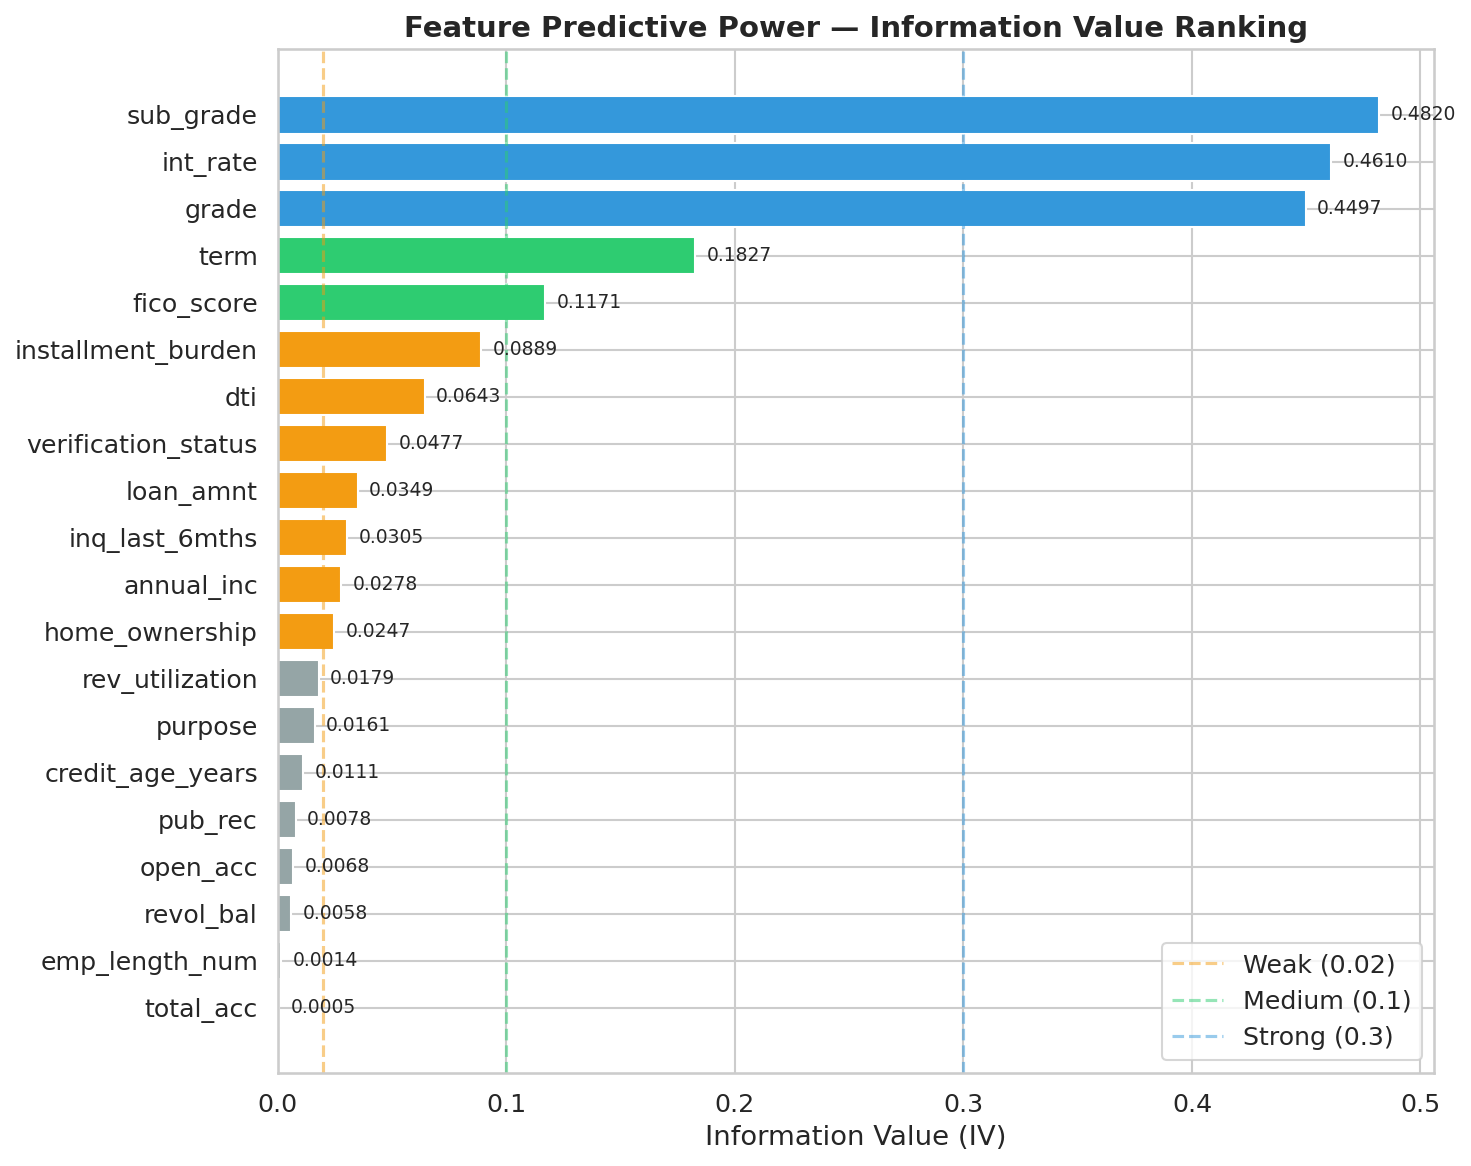
\includegraphics[keepaspectratio,alt={Ranking Information Value de variables del pipeline de features.}]{chapters/05-feature-engineering/../../assets/figures/notebooks/iv_ranking.png}}

}

\subcaption{Ranking IV de variables candidatas para el pipeline de
feature engineering.}

\end{figure}%

\end{minipage}%
%
\begin{minipage}[t]{0.50\linewidth}

\begin{figure}[H]

{\centering \pandocbounded{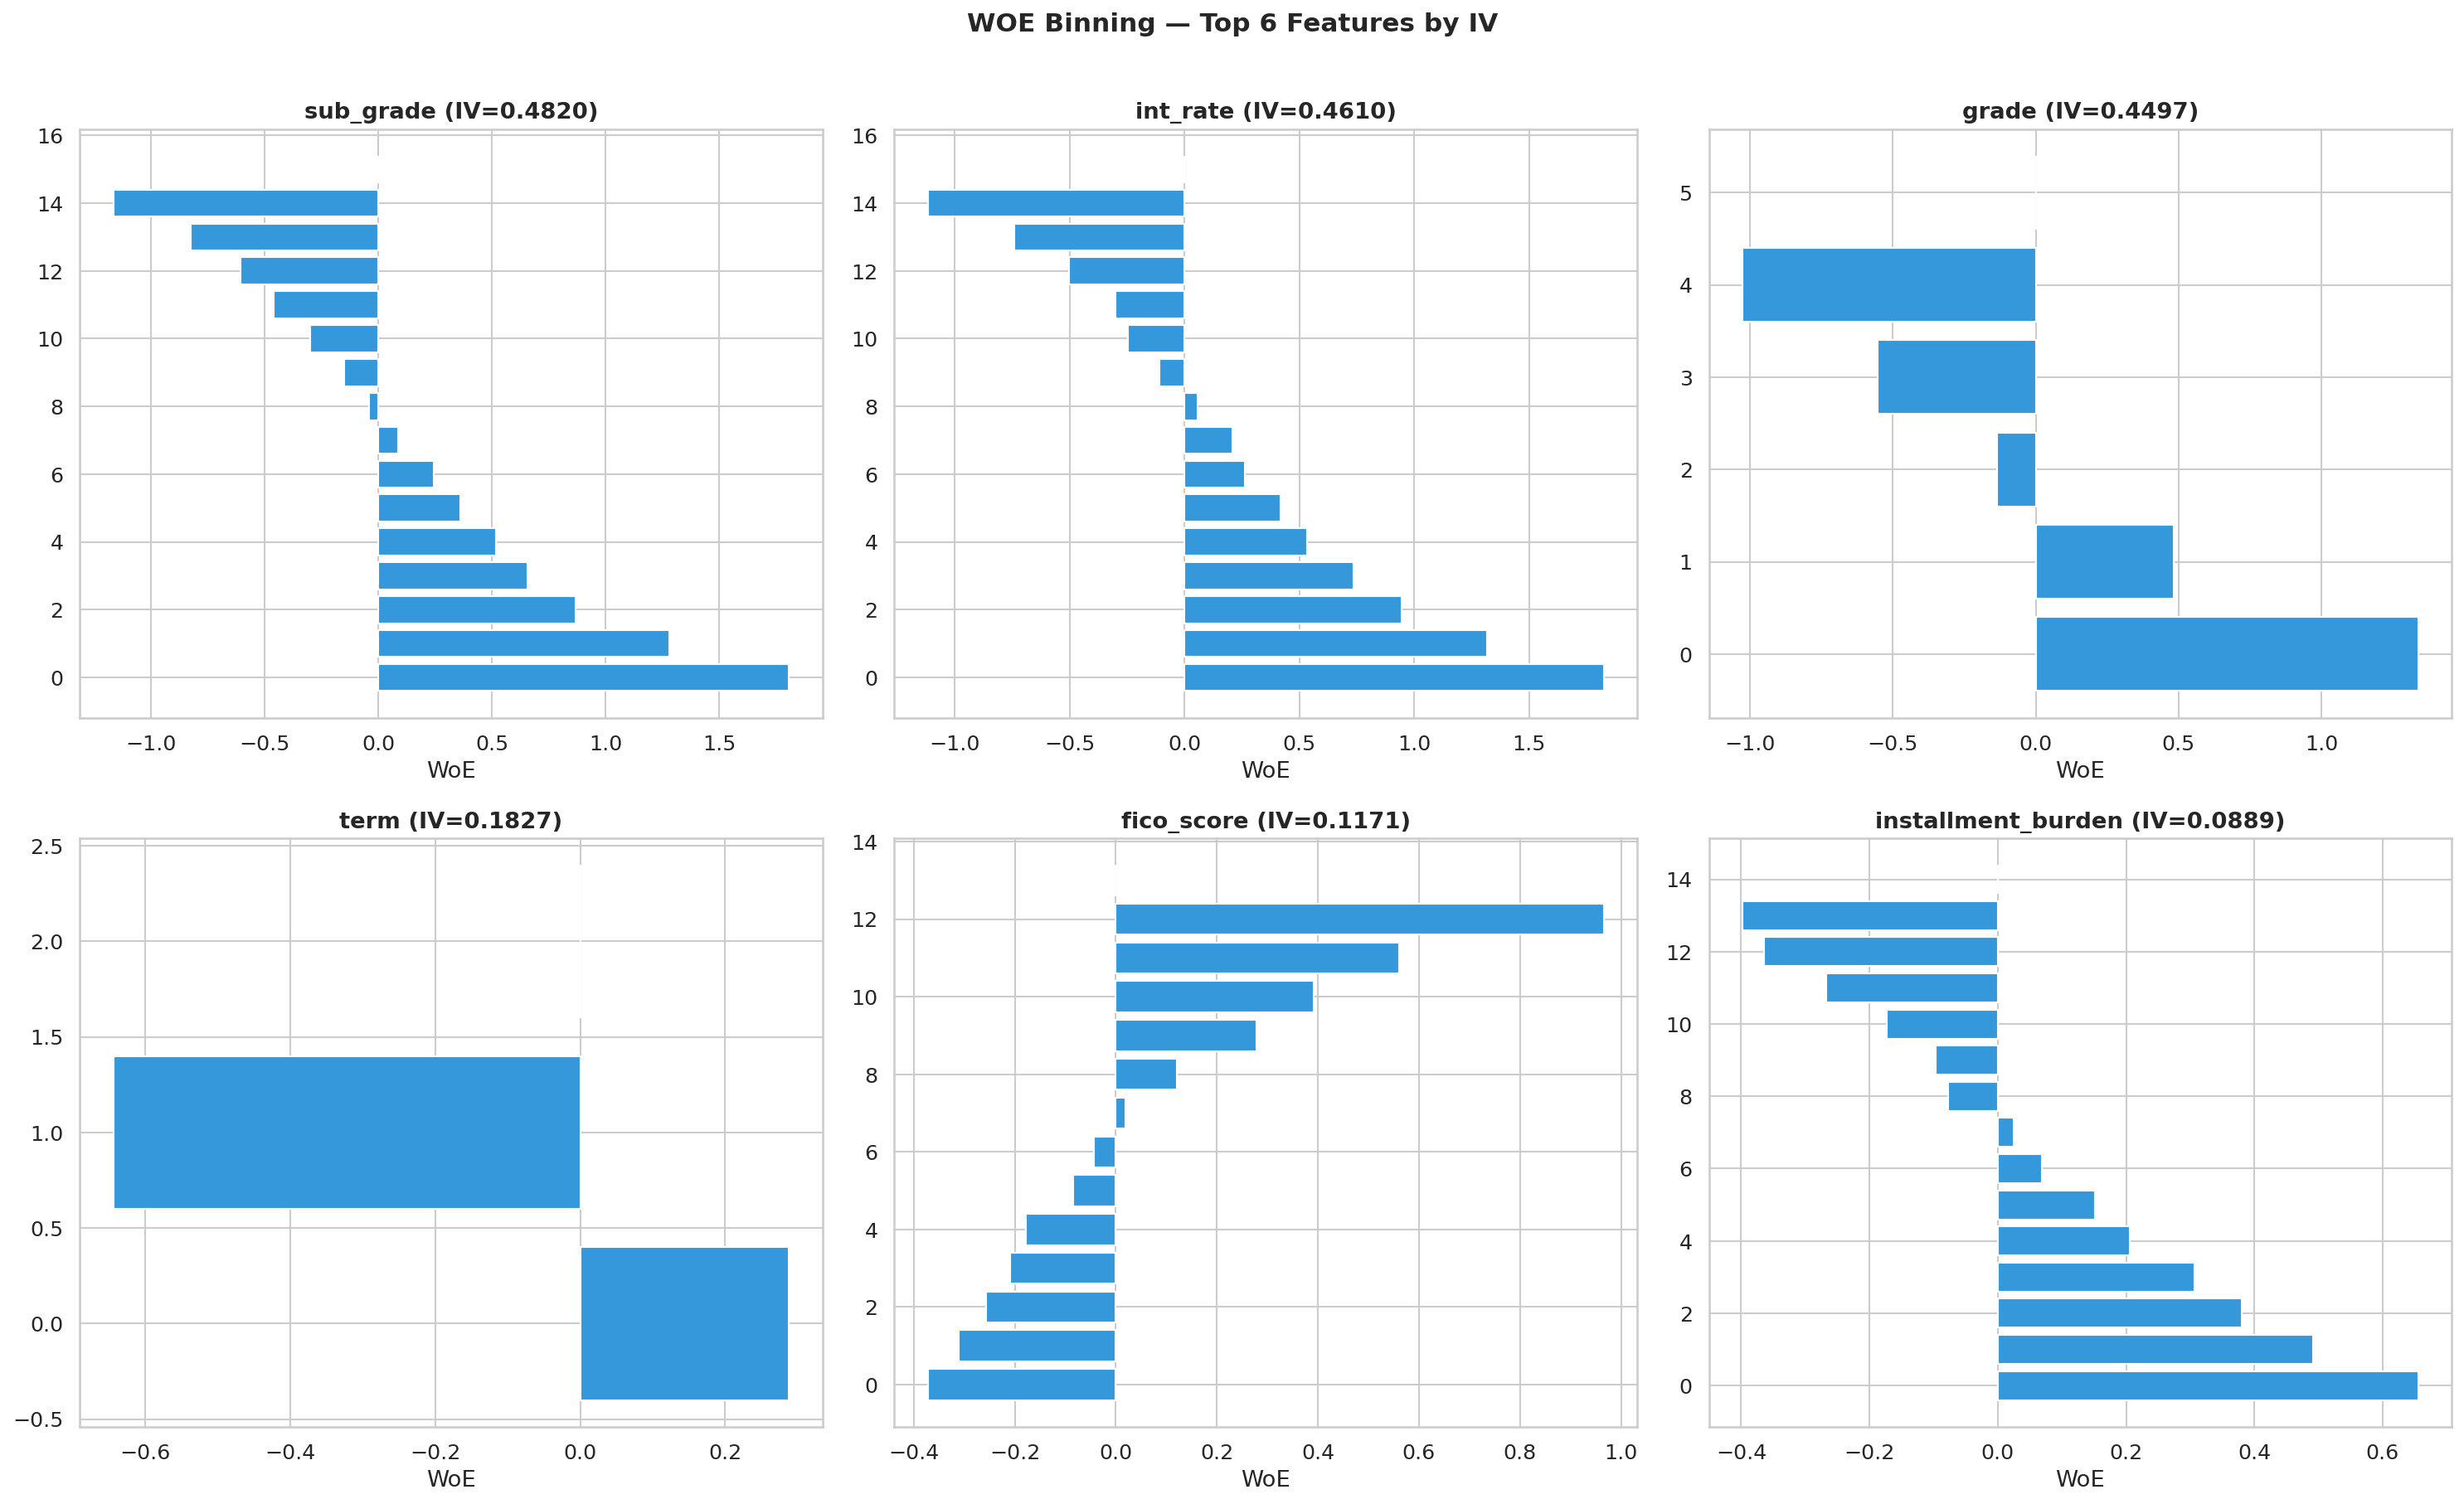
\includegraphics[keepaspectratio,alt={Comparación de bins WOE para las variables más importantes del feature engineering.}]{chapters/05-feature-engineering/../../assets/figures/notebooks/woe_binning_top6.png}}

}

\subcaption{Ejemplos de binning WOE óptimo para variables top del
modelo.}

\end{figure}%

\end{minipage}%

\end{figure*}%

\begin{longtable}[]{@{}
  >{\raggedright\arraybackslash}p{(\linewidth - 6\tabcolsep) * \real{0.2000}}
  >{\raggedright\arraybackslash}p{(\linewidth - 6\tabcolsep) * \real{0.2000}}
  >{\raggedright\arraybackslash}p{(\linewidth - 6\tabcolsep) * \real{0.2286}}
  >{\raggedright\arraybackslash}p{(\linewidth - 6\tabcolsep) * \real{0.3714}}@{}}
\caption{Etapas del pipeline de
features}\label{tbl-feature-stages}\tabularnewline
\toprule\noalign{}
\begin{minipage}[b]{\linewidth}\raggedright
Etapa
\end{minipage} & \begin{minipage}[b]{\linewidth}\raggedright
Input
\end{minipage} & \begin{minipage}[b]{\linewidth}\raggedright
Output
\end{minipage} & \begin{minipage}[b]{\linewidth}\raggedright
Herramienta
\end{minipage} \\
\midrule\noalign{}
\endfirsthead
\toprule\noalign{}
\begin{minipage}[b]{\linewidth}\raggedright
Etapa
\end{minipage} & \begin{minipage}[b]{\linewidth}\raggedright
Input
\end{minipage} & \begin{minipage}[b]{\linewidth}\raggedright
Output
\end{minipage} & \begin{minipage}[b]{\linewidth}\raggedright
Herramienta
\end{minipage} \\
\midrule\noalign{}
\endhead
\bottomrule\noalign{}
\endlastfoot
WOE/IV binning & Variables categóricas (grade, purpose, home\_ownership)
& Variables \texttt{\_woe} (numéricas, monótonas) & OptBinning (solver
CP) \\
Derivación & Variables numéricas y WOE & Ratios, logs, flags, buckets,
interacciones & \texttt{feature\_engineering.py} \\
Contrato & Todas las features candidatas & 44 features canónicas
validadas & \texttt{pd\_model\_contract.json} + Pandera \\
\end{longtable}

\chapter{WOE, IV y OptBinning}\label{sec-woe-iv}

\subsection{Motivación del Encoding
WOE}\label{motivaciuxf3n-del-encoding-woe}

Las variables categóricas en credit scoring --- como el grado de riesgo,
el propósito del préstamo o el tipo de vivienda --- no pueden usarse
directamente en modelos lineales ni en algunos modelos de ensemble. El
\textbf{Weight of Evidence} (WOE) es la transformación estándar en la
industria bancaria porque produce una codificación numérica con
propiedades deseables:

\begin{enumerate}
\def\labelenumi{\arabic{enumi}.}
\tightlist
\item
  \textbf{Monotonicidad}: La relación entre la variable WOE y el
  log-odds de default es lineal por construcción, lo que facilita la
  interpretación y la validación regulatoria.
\item
  \textbf{Poder predictivo cuantificable}: El \textbf{Information Value}
  (IV) asociado mide directamente cuánta información aporta cada
  variable para discriminar defaults de no-defaults (ver
  Capítulo~\ref{sec-ml-foundations} para las fórmulas).
\item
  \textbf{Tratamiento natural de categorías raras}: El binning agrupa
  categorías con pocos casos, evitando estimaciones inestables.
\end{enumerate}

\begin{tcolorbox}[enhanced jigsaw, arc=.35mm, bottomrule=.15mm, bottomtitle=1mm, breakable, colback=white, colbacktitle=quarto-callout-note-color!10!white, colframe=quarto-callout-note-color-frame, coltitle=black, left=2mm, leftrule=.75mm, opacityback=0, opacitybacktitle=0.6, rightrule=.15mm, title=\textcolor{quarto-callout-note-color}{\faInfo}\hspace{0.5em}{WOE vs.~One-Hot Encoding vs.~Target Encoding}, titlerule=0mm, toprule=.15mm, toptitle=1mm]

\begin{itemize}
\tightlist
\item
  \textbf{One-Hot}: Crea \(k-1\) columnas binarias para \(k\)
  categorías. Explota la dimensionalidad para variables con muchas
  categorías (Lending Club tiene 35 sub-grados).
\item
  \textbf{Target Encoding}: Reemplaza categorías por la media del
  target. Sufre de \textbf{data leakage} si no se implementa con
  regularización cuidadosa.
\item
  \textbf{WOE}: Reemplaza categorías por el log-odds ratio, calculado
  sobre bins óptimos. Es el estándar regulatorio porque produce una
  transformación interpretable, monótona y sin leakage cuando se calcula
  solo sobre el set de entrenamiento.
\end{itemize}

CatBoost maneja categorías nativamente sin necesidad de WOE, pero las
variables WOE se incluyen igualmente porque: (a) son necesarias para el
baseline de regresión logística, (b) sirven como features adicionales
para CatBoost, y (c) se usan como confusores en la estimación causal.

\end{tcolorbox}

\subsection{OptBinning: Binning Óptimo por Programación
Matemática}\label{optbinning-binning-uxf3ptimo-por-programaciuxf3n-matemuxe1tica}

El cálculo de WOE requiere primero agrupar los valores de la variable en
\textbf{bins} (intervalos para numéricas, grupos para categóricas). La
calidad de los bins determina la calidad del WOE resultante. Los
enfoques tradicionales (equal-width, equal-frequency, chi-squared
merging) son heurísticos y no garantizan optimalidad.

\textbf{OptBinning} resuelve el problema de binning como un programa de
optimización con restricciones (constraint programming, solver
\texttt{cp}), garantizando bins que maximizan el IV sujeto a
restricciones regulatorias:

\begin{itemize}
\tightlist
\item
  \textbf{Monotonía}: El WOE debe ser monótono creciente o decreciente a
  través de los bins.
\item
  \textbf{Número máximo de bins}: Típicamente 5--10 para
  interpretabilidad.
\item
  \textbf{Tamaño mínimo de bin}: Cada bin debe contener al menos un
  porcentaje mínimo de observaciones.
\end{itemize}

La implementación en \texttt{src/features/feature\_engineering.py}
utiliza OptBinning con caching:

\begin{Shaded}
\begin{Highlighting}[]
\ImportTok{from}\NormalTok{ optbinning }\ImportTok{import}\NormalTok{ OptimalBinning}

\NormalTok{optb }\OperatorTok{=}\NormalTok{ OptimalBinning(}
\NormalTok{    name}\OperatorTok{=}\NormalTok{feature,}
\NormalTok{    dtype}\OperatorTok{=}\StringTok{"numerical"} \OperatorTok{|} \StringTok{"categorical"}\NormalTok{,}
\NormalTok{    solver}\OperatorTok{=}\StringTok{"cp"}\NormalTok{,  }\CommentTok{\# constraint programming}
\NormalTok{)}
\NormalTok{optb.fit(X\_train[feature], y\_train)}
\NormalTok{woe\_values }\OperatorTok{=}\NormalTok{ optb.transform(X[feature], metric}\OperatorTok{=}\StringTok{"woe"}\NormalTok{)}
\end{Highlighting}
\end{Shaded}

Los objetos OptBinning ajustados se persisten en
\texttt{models/woe\_optbinning\_\{feature\}.pkl} para reutilización en
inferencia.

\subsection{Variables WOE del
Proyecto}\label{variables-woe-del-proyecto}

El proyecto calcula WOE para tres variables categóricas clave:

\begin{table}

\caption{\label{tbl-woe-variables}Variables transformadas con WOE
encoding}

\centering{

\begin{Shaded}
\begin{Highlighting}[]
\ImportTok{import}\NormalTok{ pandas }\ImportTok{as}\NormalTok{ pd}

\NormalTok{woe\_vars }\OperatorTok{=}\NormalTok{ [}
\NormalTok{    \{}\StringTok{"Variable original"}\NormalTok{: }\StringTok{"grade"}\NormalTok{, }\StringTok{"Variable WOE"}\NormalTok{: }\StringTok{"grade\_woe"}\NormalTok{,}
     \StringTok{"Categorías"}\NormalTok{: }\StringTok{"A, B, C, D, E, F, G (7 grados)"}\NormalTok{,}
     \StringTok{"Uso downstream"}\NormalTok{: }\StringTok{"Confusor causal, partición Mondrian, IFRS9 staging"}\NormalTok{\},}
\NormalTok{    \{}\StringTok{"Variable original"}\NormalTok{: }\StringTok{"purpose"}\NormalTok{, }\StringTok{"Variable WOE"}\NormalTok{: }\StringTok{"purpose\_woe"}\NormalTok{,}
     \StringTok{"Categorías"}\NormalTok{: }\StringTok{"debt\_consolidation, credit\_card, home\_improvement, etc. (14 categorías)"}\NormalTok{,}
     \StringTok{"Uso downstream"}\NormalTok{: }\StringTok{"Confusor causal, feature PD"}\NormalTok{\},}
\NormalTok{    \{}\StringTok{"Variable original"}\NormalTok{: }\StringTok{"home\_ownership"}\NormalTok{, }\StringTok{"Variable WOE"}\NormalTok{: }\StringTok{"home\_ownership\_woe"}\NormalTok{,}
     \StringTok{"Categorías"}\NormalTok{: }\StringTok{"MORTGAGE, RENT, OWN, OTHER (4 categorías)"}\NormalTok{,}
     \StringTok{"Uso downstream"}\NormalTok{: }\StringTok{"Confusor causal, feature PD"}\NormalTok{\},}
\NormalTok{]}

\NormalTok{pd.DataFrame(woe\_vars)}
\end{Highlighting}
\end{Shaded}

}

\end{table}%

\subsection{Ranking por Information
Value}\label{ranking-por-information-value}

El IV de cada variable se calcula como subproducto del binning óptimo y
sirve como criterio de selección de features. La interpretación estándar
(ver Tabla~\ref{tbl-iv-interpretation}) guía la decisión de qué
variables retener:

\begin{tcolorbox}[enhanced jigsaw, arc=.35mm, bottomrule=.15mm, bottomtitle=1mm, breakable, colback=white, colbacktitle=quarto-callout-tip-color!10!white, colframe=quarto-callout-tip-color-frame, coltitle=black, left=2mm, leftrule=.75mm, opacityback=0, opacitybacktitle=0.6, rightrule=.15mm, title=\textcolor{quarto-callout-tip-color}{\faLightbulb}\hspace{0.5em}{Regla práctica de IV}, titlerule=0mm, toprule=.15mm, toptitle=1mm]

Variables con IV \textgreater{} 0.50 son sospechosas de contener leakage
--- su poder predictivo es ``demasiado bueno para ser verdad''. En el
pipeline de limpieza (Sección~\ref{sec-anti-leakage}), las 35 columnas
de leakage fueron removidas \emph{antes} del cálculo de WOE, por lo que
las variables restantes tienen IV en rangos plausibles. Las variables
WOE de grade, purpose y home\_ownership tienen IV típicamente en el
rango 0.10--0.40, indicando poder predictivo medio a fuerte.

\end{tcolorbox}

El IV también se usa como criterio de ordenamiento en los notebooks de
análisis exploratorio (NB02), donde las variables se rankean por IV
descendente para identificar las más informativas antes de la selección
final de features.

\chapter{Features Derivadas: Ratios, Flags e
Interacciones}\label{sec-derived-features}

\subsection{Filosofía de Diseño}\label{filosofuxeda-de-diseuxf1o}

Las variables crudas del dataset de Lending Club capturan valores
absolutos (monto del préstamo, ingreso anual, saldo revolving), pero las
decisiones de crédito se basan en \textbf{proporciones relativas}. Un
préstamo de \$20,000 tiene riesgo muy diferente para un prestatario con
\$50,000 de ingreso anual (ratio 0.40) que para uno con \$200,000 (ratio
0.10). Las features derivadas capturan estas relaciones relativas que
son más informativas para el modelado.

El pipeline de derivación en
\texttt{src/features/feature\_engineering.py} crea cuatro tipos de
features:

\subsection{Ratios Financieros}\label{ratios-financieros}

\begin{table}

\caption{\label{tbl-ratio-features}Ratios financieros derivados}

\centering{

\begin{Shaded}
\begin{Highlighting}[]
\ImportTok{import}\NormalTok{ pandas }\ImportTok{as}\NormalTok{ pd}

\NormalTok{ratios }\OperatorTok{=}\NormalTok{ [}
\NormalTok{    \{}\StringTok{"Feature"}\NormalTok{: }\StringTok{"loan\_to\_income"}\NormalTok{, }\StringTok{"Fórmula"}\NormalTok{: }\StringTok{"loan\_amnt / annual\_inc"}\NormalTok{,}
     \StringTok{"Interpretación"}\NormalTok{: }\StringTok{"Carga del préstamo relativa al ingreso. Valores \textgreater{} 0.50 indican alto apalancamiento"}\NormalTok{\},}
\NormalTok{    \{}\StringTok{"Feature"}\NormalTok{: }\StringTok{"installment\_burden"}\NormalTok{, }\StringTok{"Fórmula"}\NormalTok{: }\StringTok{"installment / (annual\_inc / 12)"}\NormalTok{,}
     \StringTok{"Interpretación"}\NormalTok{: }\StringTok{"Cuota mensual como fracción del ingreso mensual"}\NormalTok{\},}
\NormalTok{    \{}\StringTok{"Feature"}\NormalTok{: }\StringTok{"rev\_utilization"}\NormalTok{, }\StringTok{"Fórmula"}\NormalTok{: }\StringTok{"revol\_util / 100"}\NormalTok{,}
     \StringTok{"Interpretación"}\NormalTok{: }\StringTok{"Utilización de líneas revolving (0–1). Valores \textgreater{} 0.80 son señal de estrés"}\NormalTok{\},}
\NormalTok{    \{}\StringTok{"Feature"}\NormalTok{: }\StringTok{"revol\_bal\_to\_income"}\NormalTok{, }\StringTok{"Fórmula"}\NormalTok{: }\StringTok{"revol\_bal / annual\_inc"}\NormalTok{,}
     \StringTok{"Interpretación"}\NormalTok{: }\StringTok{"Deuda revolving relativa al ingreso"}\NormalTok{\},}
\NormalTok{    \{}\StringTok{"Feature"}\NormalTok{: }\StringTok{"open\_acc\_ratio"}\NormalTok{, }\StringTok{"Fórmula"}\NormalTok{: }\StringTok{"open\_acc / total\_acc"}\NormalTok{,}
     \StringTok{"Interpretación"}\NormalTok{: }\StringTok{"Proporción de cuentas activas. Valores altos indican búsqueda activa de crédito"}\NormalTok{\},}
\NormalTok{    \{}\StringTok{"Feature"}\NormalTok{: }\StringTok{"il\_ratio"}\NormalTok{, }\StringTok{"Fórmula"}\NormalTok{: }\StringTok{"Ratio de deuda installment sobre total"}\NormalTok{,}
     \StringTok{"Interpretación"}\NormalTok{: }\StringTok{"Concentración en deuda de cuotas fijas vs. revolving"}\NormalTok{\},}
\NormalTok{    \{}\StringTok{"Feature"}\NormalTok{: }\StringTok{"high\_util\_pct"}\NormalTok{, }\StringTok{"Fórmula"}\NormalTok{: }\StringTok{"Porcentaje de líneas con utilización \textgreater{} 80\%"}\NormalTok{,}
     \StringTok{"Interpretación"}\NormalTok{: }\StringTok{"Diversificación del estrés crediticio entre líneas"}\NormalTok{\},}
\NormalTok{]}

\NormalTok{pd.DataFrame(ratios)}
\end{Highlighting}
\end{Shaded}

}

\end{table}%

\subsection{Transformaciones
Logarítmicas}\label{transformaciones-logaruxedtmicas}

Las variables financieras tienen distribuciones fuertemente sesgadas a
la derecha (muchos prestatarios con ingresos modestos, pocos con
ingresos muy altos). Las transformaciones logarítmicas estabilizan la
varianza y reducen la influencia de valores extremos:

\begin{longtable}[]{@{}
  >{\raggedright\arraybackslash}p{(\linewidth - 4\tabcolsep) * \real{0.2727}}
  >{\raggedright\arraybackslash}p{(\linewidth - 4\tabcolsep) * \real{0.2727}}
  >{\raggedright\arraybackslash}p{(\linewidth - 4\tabcolsep) * \real{0.4545}}@{}}
\caption{Transformaciones
logarítmicas}\label{tbl-log-features}\tabularnewline
\toprule\noalign{}
\begin{minipage}[b]{\linewidth}\raggedright
Feature
\end{minipage} & \begin{minipage}[b]{\linewidth}\raggedright
Fórmula
\end{minipage} & \begin{minipage}[b]{\linewidth}\raggedright
Justificación
\end{minipage} \\
\midrule\noalign{}
\endfirsthead
\toprule\noalign{}
\begin{minipage}[b]{\linewidth}\raggedright
Feature
\end{minipage} & \begin{minipage}[b]{\linewidth}\raggedright
Fórmula
\end{minipage} & \begin{minipage}[b]{\linewidth}\raggedright
Justificación
\end{minipage} \\
\midrule\noalign{}
\endhead
\bottomrule\noalign{}
\endlastfoot
\texttt{log\_annual\_inc} & \(\log(1 + \text{annual\_inc})\) & Ingreso
tiene cola derecha pesada \\
\texttt{log\_revol\_bal} & \(\log(1 + \text{revol\_bal})\) & Saldo
revolving varía de \$0 a \textgreater{} \$100K \\
\end{longtable}

El \(+1\) evita el \(\log(0)\) para prestatarios sin saldo revolving.

\subsection{Flags Binarias}\label{flags-binarias}

Las flags capturan la presencia o ausencia de señales de riesgo
discretas:

\begin{table}

\caption{\label{tbl-flag-features}Features binarias (flags) de señal de
riesgo}

\centering{

\begin{Shaded}
\begin{Highlighting}[]
\NormalTok{flags }\OperatorTok{=}\NormalTok{ [}
\NormalTok{    \{}\StringTok{"Feature"}\NormalTok{: }\StringTok{"has\_delinq\_2yrs"}\NormalTok{, }\StringTok{"Condición"}\NormalTok{: }\StringTok{"delinq\_2yrs \textgreater{} 0"}\NormalTok{,}
     \StringTok{"Señal"}\NormalTok{: }\StringTok{"Morosidad reciente en los últimos 2 años"}\NormalTok{\},}
\NormalTok{    \{}\StringTok{"Feature"}\NormalTok{: }\StringTok{"has\_pub\_rec"}\NormalTok{, }\StringTok{"Condición"}\NormalTok{: }\StringTok{"pub\_rec \textgreater{} 0"}\NormalTok{,}
     \StringTok{"Señal"}\NormalTok{: }\StringTok{"Registro público derogatorio (quiebra, juicio)"}\NormalTok{\},}
\NormalTok{    \{}\StringTok{"Feature"}\NormalTok{: }\StringTok{"has\_bankruptcy"}\NormalTok{, }\StringTok{"Condición"}\NormalTok{: }\StringTok{"pub\_rec\_bankruptcies \textgreater{} 0"}\NormalTok{,}
     \StringTok{"Señal"}\NormalTok{: }\StringTok{"Quiebra personal previa"}\NormalTok{\},}
\NormalTok{    \{}\StringTok{"Feature"}\NormalTok{: }\StringTok{"has\_recent\_inq"}\NormalTok{, }\StringTok{"Condición"}\NormalTok{: }\StringTok{"inq\_last\_6mths \textgreater{} 0"}\NormalTok{,}
     \StringTok{"Señal"}\NormalTok{: }\StringTok{"Consulta de crédito en últimos 6 meses (búsqueda activa)"}\NormalTok{\},}
\NormalTok{    \{}\StringTok{"Feature"}\NormalTok{: }\StringTok{"has\_mortgage"}\NormalTok{, }\StringTok{"Condición"}\NormalTok{: }\StringTok{"mort\_acc \textgreater{} 0"}\NormalTok{,}
     \StringTok{"Señal"}\NormalTok{: }\StringTok{"Tiene hipoteca (indicador de estabilidad financiera)"}\NormalTok{\},}
\NormalTok{    \{}\StringTok{"Feature"}\NormalTok{: }\StringTok{"many\_recent\_opens"}\NormalTok{, }\StringTok{"Condición"}\NormalTok{: }\StringTok{"open\_acc \textgreater{} umbral"}\NormalTok{,}
     \StringTok{"Señal"}\NormalTok{: }\StringTok{"Muchas cuentas abiertas recientemente"}\NormalTok{\},}
\NormalTok{    \{}\StringTok{"Feature"}\NormalTok{: }\StringTok{"recent\_chargeoff"}\NormalTok{, }\StringTok{"Condición"}\NormalTok{: }\StringTok{"chargeoff\_within\_12\_mths \textgreater{} 0"}\NormalTok{,}
     \StringTok{"Señal"}\NormalTok{: }\StringTok{"Pérdida crediticia reciente (12 meses)"}\NormalTok{\},}
\NormalTok{    \{}\StringTok{"Feature"}\NormalTok{: }\StringTok{"early\_delinq"}\NormalTok{, }\StringTok{"Condición"}\NormalTok{: }\StringTok{"delinq\_2yrs \textgreater{} 0"}\NormalTok{,}
     \StringTok{"Señal"}\NormalTok{: }\StringTok{"Historial temprano de morosidad"}\NormalTok{\},}
\NormalTok{]}

\NormalTok{pd.DataFrame(flags)}
\end{Highlighting}
\end{Shaded}

}

\end{table}%

\begin{tcolorbox}[enhanced jigsaw, arc=.35mm, bottomrule=.15mm, bottomtitle=1mm, breakable, colback=white, colbacktitle=quarto-callout-note-color!10!white, colframe=quarto-callout-note-color-frame, coltitle=black, left=2mm, leftrule=.75mm, opacityback=0, opacitybacktitle=0.6, rightrule=.15mm, title=\textcolor{quarto-callout-note-color}{\faInfo}\hspace{0.5em}{Flags vs.~variables continuas}, titlerule=0mm, toprule=.15mm, toptitle=1mm]

Las flags pueden parecer redundantes con las variables continuas
subyacentes (por ejemplo, \texttt{has\_delinq\_2yrs}
vs.~\texttt{delinq\_2yrs}). Sin embargo, para modelos lineales como la
regresión logística, la flag captura el \emph{salto discreto} en riesgo
entre ``cero delinquencias'' y ``al menos una'', que es la
discontinuidad más informativa. CatBoost puede descubrir esta
discontinuidad automáticamente, pero incluir la flag explícitamente
facilita la interpretabilidad y la consistencia entre modelos.

\end{tcolorbox}

\subsection{Features Temporales}\label{features-temporales}

\begin{table}

\caption{\label{tbl-temporal-features}Features temporales derivadas}

\centering{

\begin{Shaded}
\begin{Highlighting}[]
\NormalTok{temporal }\OperatorTok{=}\NormalTok{ [}
\NormalTok{    \{}\StringTok{"Feature"}\NormalTok{: }\StringTok{"credit\_history\_months"}\NormalTok{, }\StringTok{"Fórmula"}\NormalTok{: }\StringTok{"(issue\_d {-} earliest\_cr\_line).days / 30"}\NormalTok{,}
     \StringTok{"Interpretación"}\NormalTok{: }\StringTok{"Antigüedad del historial crediticio en meses"}\NormalTok{\},}
\NormalTok{    \{}\StringTok{"Feature"}\NormalTok{: }\StringTok{"credit\_age\_years"}\NormalTok{, }\StringTok{"Fórmula"}\NormalTok{: }\StringTok{"credit\_history\_months / 12"}\NormalTok{,}
     \StringTok{"Interpretación"}\NormalTok{: }\StringTok{"Versión en años para interpretabilidad"}\NormalTok{\},}
\NormalTok{    \{}\StringTok{"Feature"}\NormalTok{: }\StringTok{"fico\_score"}\NormalTok{, }\StringTok{"Fórmula"}\NormalTok{: }\StringTok{"(fico\_range\_low + fico\_range\_high) / 2"}\NormalTok{,}
     \StringTok{"Interpretación"}\NormalTok{: }\StringTok{"Punto medio del rango FICO reportado"}\NormalTok{\},}
\NormalTok{    \{}\StringTok{"Feature"}\NormalTok{: }\StringTok{"delinq\_severity"}\NormalTok{, }\StringTok{"Fórmula"}\NormalTok{: }\StringTok{"Combinación de morosidades por tipo"}\NormalTok{,}
     \StringTok{"Interpretación"}\NormalTok{: }\StringTok{"Índice compuesto de severidad de morosidad"}\NormalTok{\},}
\NormalTok{    \{}\StringTok{"Feature"}\NormalTok{: }\StringTok{"delinq\_recency"}\NormalTok{, }\StringTok{"Fórmula"}\NormalTok{: }\StringTok{"Inverso de meses desde última morosidad"}\NormalTok{,}
     \StringTok{"Interpretación"}\NormalTok{: }\StringTok{"Más alto = morosidad más reciente"}\NormalTok{\},}
\NormalTok{]}

\NormalTok{pd.DataFrame(temporal)}
\end{Highlighting}
\end{Shaded}

}

\end{table}%

\subsection{Buckets e Interacciones}\label{buckets-e-interacciones}

Las variables de \textbf{bucket} discretizan continuas en categorías
interpretables:

\begin{itemize}
\tightlist
\item
  \texttt{int\_rate\_bucket}: very\_low (0--8\%), low (8--12\%), medium
  (12--16\%), high (16--20\%), very\_high (\textgreater20\%)
\item
  \texttt{dti\_bucket}: low (0--10), moderate (10--20), high (20--30),
  very\_high (30--40), extreme (\textgreater40)
\item
  \texttt{fico\_bucket}: Discretización del score FICO en bandas
\end{itemize}

Las \textbf{interacciones} capturan efectos multiplicativos:

\begin{longtable}[]{@{}
  >{\raggedright\arraybackslash}p{(\linewidth - 4\tabcolsep) * \real{0.2812}}
  >{\raggedright\arraybackslash}p{(\linewidth - 4\tabcolsep) * \real{0.3750}}
  >{\raggedright\arraybackslash}p{(\linewidth - 4\tabcolsep) * \real{0.3438}}@{}}
\caption{Features de
interacción}\label{tbl-interaction-features}\tabularnewline
\toprule\noalign{}
\begin{minipage}[b]{\linewidth}\raggedright
Feature
\end{minipage} & \begin{minipage}[b]{\linewidth}\raggedright
Componentes
\end{minipage} & \begin{minipage}[b]{\linewidth}\raggedright
Intuición
\end{minipage} \\
\midrule\noalign{}
\endfirsthead
\toprule\noalign{}
\begin{minipage}[b]{\linewidth}\raggedright
Feature
\end{minipage} & \begin{minipage}[b]{\linewidth}\raggedright
Componentes
\end{minipage} & \begin{minipage}[b]{\linewidth}\raggedright
Intuición
\end{minipage} \\
\midrule\noalign{}
\endhead
\bottomrule\noalign{}
\endlastfoot
\texttt{int\_rate\_bucket\_\_grade} & int\_rate\_bucket × grade &
Captura si la tasa es alta \emph{para su grado} \\
\texttt{loan\_to\_income\_sq} & loan\_to\_income² & Efecto no lineal
convexo del apalancamiento \\
\texttt{fico\_x\_dti} & fico\_score × dti & Interacción entre calidad
crediticia y carga de deuda \\
\end{longtable}

\begin{tcolorbox}[enhanced jigsaw, arc=.35mm, bottomrule=.15mm, bottomtitle=1mm, breakable, colback=white, colbacktitle=quarto-callout-tip-color!10!white, colframe=quarto-callout-tip-color-frame, coltitle=black, left=2mm, leftrule=.75mm, opacityback=0, opacitybacktitle=0.6, rightrule=.15mm, title=\textcolor{quarto-callout-tip-color}{\faLightbulb}\hspace{0.5em}{¿Son necesarias las interacciones para CatBoost?}, titlerule=0mm, toprule=.15mm, toptitle=1mm]

CatBoost y otros modelos de ensemble basados en árboles descubren
interacciones automáticamente durante el entrenamiento. Sin embargo,
proporcionar interacciones explícitas tiene dos beneficios: (1) facilita
la interpretabilidad vía SHAP (la importancia de \texttt{fico\_x\_dti}
se lee directamente), y (2) beneficia al modelo de regresión logística
baseline que no captura interacciones automáticamente.

\end{tcolorbox}

\chapter{Contrato de Features y Validación}\label{sec-feature-contract}

\subsection{El Concepto de Contrato
Canónico}\label{el-concepto-de-contrato-canuxf3nico}

En un pipeline de ML con múltiples etapas (features → modelo →
calibración → conformal → optimización), la consistencia de features
entre etapas es crítica. Si el modelo se entrena con 44 features en
cierto orden y la inferencia recibe 43 en orden diferente, los
resultados son silenciosamente incorrectos --- no hay error de runtime,
solo predicciones degradadas que solo se detectan cuando se monitorearan
métricas en producción.

El \textbf{contrato canónico de features}
(\texttt{models/pd\_model\_contract.json}) resuelve este problema
documentando la interfaz exacta del modelo:

\begin{table}

\caption{\label{tbl-contract-summary}Resumen del contrato canónico de
features}

\centering{

\begin{Shaded}
\begin{Highlighting}[]
\ImportTok{import}\NormalTok{ sys}
\ImportTok{from}\NormalTok{ pathlib }\ImportTok{import}\NormalTok{ Path}

\NormalTok{sys.path.insert(}\DecValTok{0}\NormalTok{, }\BuiltInTok{str}\NormalTok{(Path.cwd().parent }\ControlFlowTok{if}\NormalTok{ Path.cwd().name }\OperatorTok{==} \StringTok{"book"} \ControlFlowTok{else}\NormalTok{ Path.cwd()))}
\ImportTok{from}\NormalTok{ book.\_helpers.load\_artifacts }\ImportTok{import}\NormalTok{ try\_load\_json}

\ImportTok{import}\NormalTok{ pandas }\ImportTok{as}\NormalTok{ pd}

\NormalTok{contract }\OperatorTok{=}\NormalTok{ try\_load\_json(}\StringTok{"pd\_model\_contract"}\NormalTok{, directory}\OperatorTok{=}\StringTok{"models"}\NormalTok{, default}\OperatorTok{=}\NormalTok{\{\})}

\NormalTok{contract\_summary }\OperatorTok{=}\NormalTok{ [}
\NormalTok{    \{}\StringTok{"Atributo"}\NormalTok{: }\StringTok{"Features totales"}\NormalTok{, }\StringTok{"Valor"}\NormalTok{: }\BuiltInTok{str}\NormalTok{(contract.get(}\StringTok{"n\_features"}\NormalTok{, }\StringTok{"N/A"}\NormalTok{))\},}
\NormalTok{    \{}\StringTok{"Atributo"}\NormalTok{: }\StringTok{"Features categóricas"}\NormalTok{, }\StringTok{"Valor"}\NormalTok{: }\BuiltInTok{str}\NormalTok{(}\BuiltInTok{len}\NormalTok{(contract.get(}\StringTok{"categorical\_features"}\NormalTok{, [])))\},}
\NormalTok{    \{}\StringTok{"Atributo"}\NormalTok{: }\StringTok{"Features numéricas"}\NormalTok{, }\StringTok{"Valor"}\NormalTok{: }\BuiltInTok{str}\NormalTok{(contract.get(}\StringTok{"n\_features"}\NormalTok{, }\DecValTok{0}\NormalTok{) }\OperatorTok{{-}} \BuiltInTok{len}\NormalTok{(contract.get(}\StringTok{"categorical\_features"}\NormalTok{, [])))\},}
\NormalTok{    \{}\StringTok{"Atributo"}\NormalTok{: }\StringTok{"Modelo canónico"}\NormalTok{, }\StringTok{"Valor"}\NormalTok{: contract.get(}\StringTok{"model\_path"}\NormalTok{, }\StringTok{"N/A"}\NormalTok{)\},}
\NormalTok{    \{}\StringTok{"Atributo"}\NormalTok{: }\StringTok{"Calibrador"}\NormalTok{, }\StringTok{"Valor"}\NormalTok{: contract.get(}\StringTok{"calibrator\_path"}\NormalTok{, }\StringTok{"N/A"}\NormalTok{)\},}
\NormalTok{]}

\NormalTok{pd.DataFrame(contract\_summary)}
\end{Highlighting}
\end{Shaded}

}

\end{table}%

\subsection{Estructura del Contrato}\label{estructura-del-contrato}

El contrato JSON contiene cuatro secciones:

\textbf{1. Lista ordenada de features} (\texttt{feature\_names}): Las 44
features exactas que el modelo espera, en el orden exacto en que fueron
presentadas durante el entrenamiento. Cualquier discrepancia en nombres
o en orden invalida las predicciones.

\textbf{2. Features categóricas} (\texttt{categorical\_features}): Las 9
features que CatBoost trata como categorías nativas:

\begin{table}

\caption{\label{tbl-categorical-features}Features categóricas del
contrato (CatBoost nativo)}

\centering{

\begin{Shaded}
\begin{Highlighting}[]
\NormalTok{cat\_features }\OperatorTok{=}\NormalTok{ contract.get(}\StringTok{"categorical\_features"}\NormalTok{, [])}
\NormalTok{cat\_df }\OperatorTok{=}\NormalTok{ pd.DataFrame(\{}\StringTok{"Feature categórica"}\NormalTok{: cat\_features, }\StringTok{"\#"}\NormalTok{: }\BuiltInTok{range}\NormalTok{(}\DecValTok{1}\NormalTok{, }\BuiltInTok{len}\NormalTok{(cat\_features) }\OperatorTok{+} \DecValTok{1}\NormalTok{)\})}
\NormalTok{cat\_df}
\end{Highlighting}
\end{Shaded}

}

\end{table}%

CatBoost aplica target encoding con ordered boosting a estas features
internamente. No requieren one-hot encoding ni WOE --- el modelo las
consume en su formato original (strings o categorías pandas).

\textbf{3. Shapes de los splits} (\texttt{split\_shapes}): Dimensiones
de train, calibración y test al momento del entrenamiento, para
verificar que los datasets no han cambiado.

\textbf{4. Features faltantes por split}
(\texttt{split\_missing\_features}): Listas vacías si todos los splits
contienen todas las features del contrato. Si algún split tiene features
faltantes, esta sección lo documenta explícitamente.

\subsection{Pandera: Validación de Schemas en
Runtime}\label{pandera-validaciuxf3n-de-schemas-en-runtime}

El contrato JSON es una especificación estática. Para validación
dinámica en tiempo de ejecución, el pipeline usa \textbf{Pandera}
(\texttt{src/features/schemas.py}) con schemas tipados para cada dataset
analítico:

\begin{table}

\caption{\label{tbl-pandera-schemas}Schemas Pandera para validación de
datos}

\centering{

\begin{Shaded}
\begin{Highlighting}[]
\NormalTok{schemas }\OperatorTok{=}\NormalTok{ [}
\NormalTok{    \{}\StringTok{"Schema"}\NormalTok{: }\StringTok{"loan\_master\_schema"}\NormalTok{, }\StringTok{"Dataset"}\NormalTok{: }\StringTok{"loan\_master.parquet"}\NormalTok{,}
     \StringTok{"Validaciones clave"}\NormalTok{: }\StringTok{"loan\_amnt \textgreater{} 0, default\_flag ∈ \{0,1\}, int\_rate ∈ [0,100], dti ∈ [0,999]"}\NormalTok{\},}
\NormalTok{    \{}\StringTok{"Schema"}\NormalTok{: }\StringTok{"time\_series\_schema"}\NormalTok{, }\StringTok{"Dataset"}\NormalTok{: }\StringTok{"time\_series.parquet"}\NormalTok{,}
     \StringTok{"Validaciones clave"}\NormalTok{: }\StringTok{"ds es datetime, y ∈ [0,1] (default\_rate), loan\_count \textgreater{} 0"}\NormalTok{\},}
\NormalTok{    \{}\StringTok{"Schema"}\NormalTok{: }\StringTok{"ead\_schema"}\NormalTok{, }\StringTok{"Dataset"}\NormalTok{: }\StringTok{"ead\_dataset.parquet"}\NormalTok{,}
     \StringTok{"Validaciones clave"}\NormalTok{: }\StringTok{"default\_flag = 1 (solo defaults), loan\_amnt \textgreater{} 0"}\NormalTok{\},}
\NormalTok{    \{}\StringTok{"Schema"}\NormalTok{: }\StringTok{"prediction\_schema"}\NormalTok{, }\StringTok{"Dataset"}\NormalTok{: }\StringTok{"Predicciones PD"}\NormalTok{,}
     \StringTok{"Validaciones clave"}\NormalTok{: }\StringTok{"pd\_low ≤ pd\_point ≤ pd\_high, todos en [0,1]"}\NormalTok{\},}
\NormalTok{]}

\NormalTok{pd.DataFrame(schemas)}
\end{Highlighting}
\end{Shaded}

}

\end{table}%

El \texttt{prediction\_schema} incluye una validación crítica para
predicción conformal: la relación de orden
\texttt{pd\_low\ ≤\ pd\_point\ ≤\ pd\_high} se verifica con checks de
DataFrame que cruzan columnas. Si un intervalo conformal tiene el límite
inferior por encima del punto estimado, el schema falla y detiene el
pipeline.

\begin{tcolorbox}[enhanced jigsaw, arc=.35mm, bottomrule=.15mm, bottomtitle=1mm, breakable, colback=white, colbacktitle=quarto-callout-note-color!10!white, colframe=quarto-callout-note-color-frame, coltitle=black, left=2mm, leftrule=.75mm, opacityback=0, opacitybacktitle=0.6, rightrule=.15mm, title=\textcolor{quarto-callout-note-color}{\faInfo}\hspace{0.5em}{Validación estricta vs.~tolerante}, titlerule=0mm, toprule=.15mm, toptitle=1mm]

Los schemas usan \texttt{strict=False}, lo que permite columnas
adicionales no especificadas en el schema. Esto es deliberado: a medida
que el pipeline evoluciona, nuevas features pueden agregarse sin romper
las validaciones existentes. Solo las columnas críticas se validan
estrictamente; el resto se ignora. Si se requiriera validación estricta
(no permitir columnas extra), se cambiaría a \texttt{strict=True}.

\end{tcolorbox}

\subsection{Flujo de Validación}\label{flujo-de-validaciuxf3n}

La validación se integra en el pipeline como un \emph{gate} entre
etapas:

\begin{verbatim}
Feature Engineering → [Pandera loan_master_schema] → Train PD Model
                                                           ↓
                                                   [Contrato JSON]
                                                           ↓
Conformal Intervals → [Pandera prediction_schema] → Portfolio Optimizer
\end{verbatim}

Si una validación falla, el pipeline se detiene con un error descriptivo
que indica qué columna, qué regla y qué valores violaron el schema. Esto
es preferible a dejar que un error de datos se propague silenciosamente
hasta producir predicciones incorrectas o portafolios subóptimos.

\begin{tcolorbox}[enhanced jigsaw, arc=.35mm, bottomrule=.15mm, bottomtitle=1mm, breakable, colback=white, colbacktitle=quarto-callout-warning-color!10!white, colframe=quarto-callout-warning-color-frame, coltitle=black, left=2mm, leftrule=.75mm, opacityback=0, opacitybacktitle=0.6, rightrule=.15mm, title=\textcolor{quarto-callout-warning-color}{\faExclamationTriangle}\hspace{0.5em}{Manejo de NaN}, titlerule=0mm, toprule=.15mm, toptitle=1mm]

El contrato permite NaN en la mayoría de features numéricas
(\texttt{nullable=True}) porque CatBoost trata los valores faltantes
como un valor informativo adicional, asignándolos a la rama óptima de
cada split. Sin embargo, \texttt{loan\_amnt} y \texttt{default\_flag}
son no-nullable --- un valor faltante en estas columnas indica un error
de datos que debe corregirse antes de proceder.

Para la regresión logística baseline, los NaN se reemplazan con
\texttt{fillna(0)} como estrategia simple. Esta asimetría en el
tratamiento de NaN es una de las ventajas de CatBoost sobre modelos
lineales para datos financieros con missing values informativos.

\end{tcolorbox}

\chapter{Modelado de PD y
Calibración}\label{modelado-de-pd-y-calibraciuxf3n}

El modelo de Probabilidad de Default (PD) es el corazón predictivo del
pipeline. Este capítulo documenta la estrategia completa de modelado:
desde el baseline interpretable de regresión logística hasta el modelo
CatBoost optimizado con Optuna, pasando por la selección automática del
calibrador y la designación del modelo champion.

La estrategia de modelado sigue un principio de \textbf{complejidad
incremental}:

\begin{figure*}

\begin{minipage}[t]{0.50\linewidth}

\begin{figure}[H]

{\centering \pandocbounded{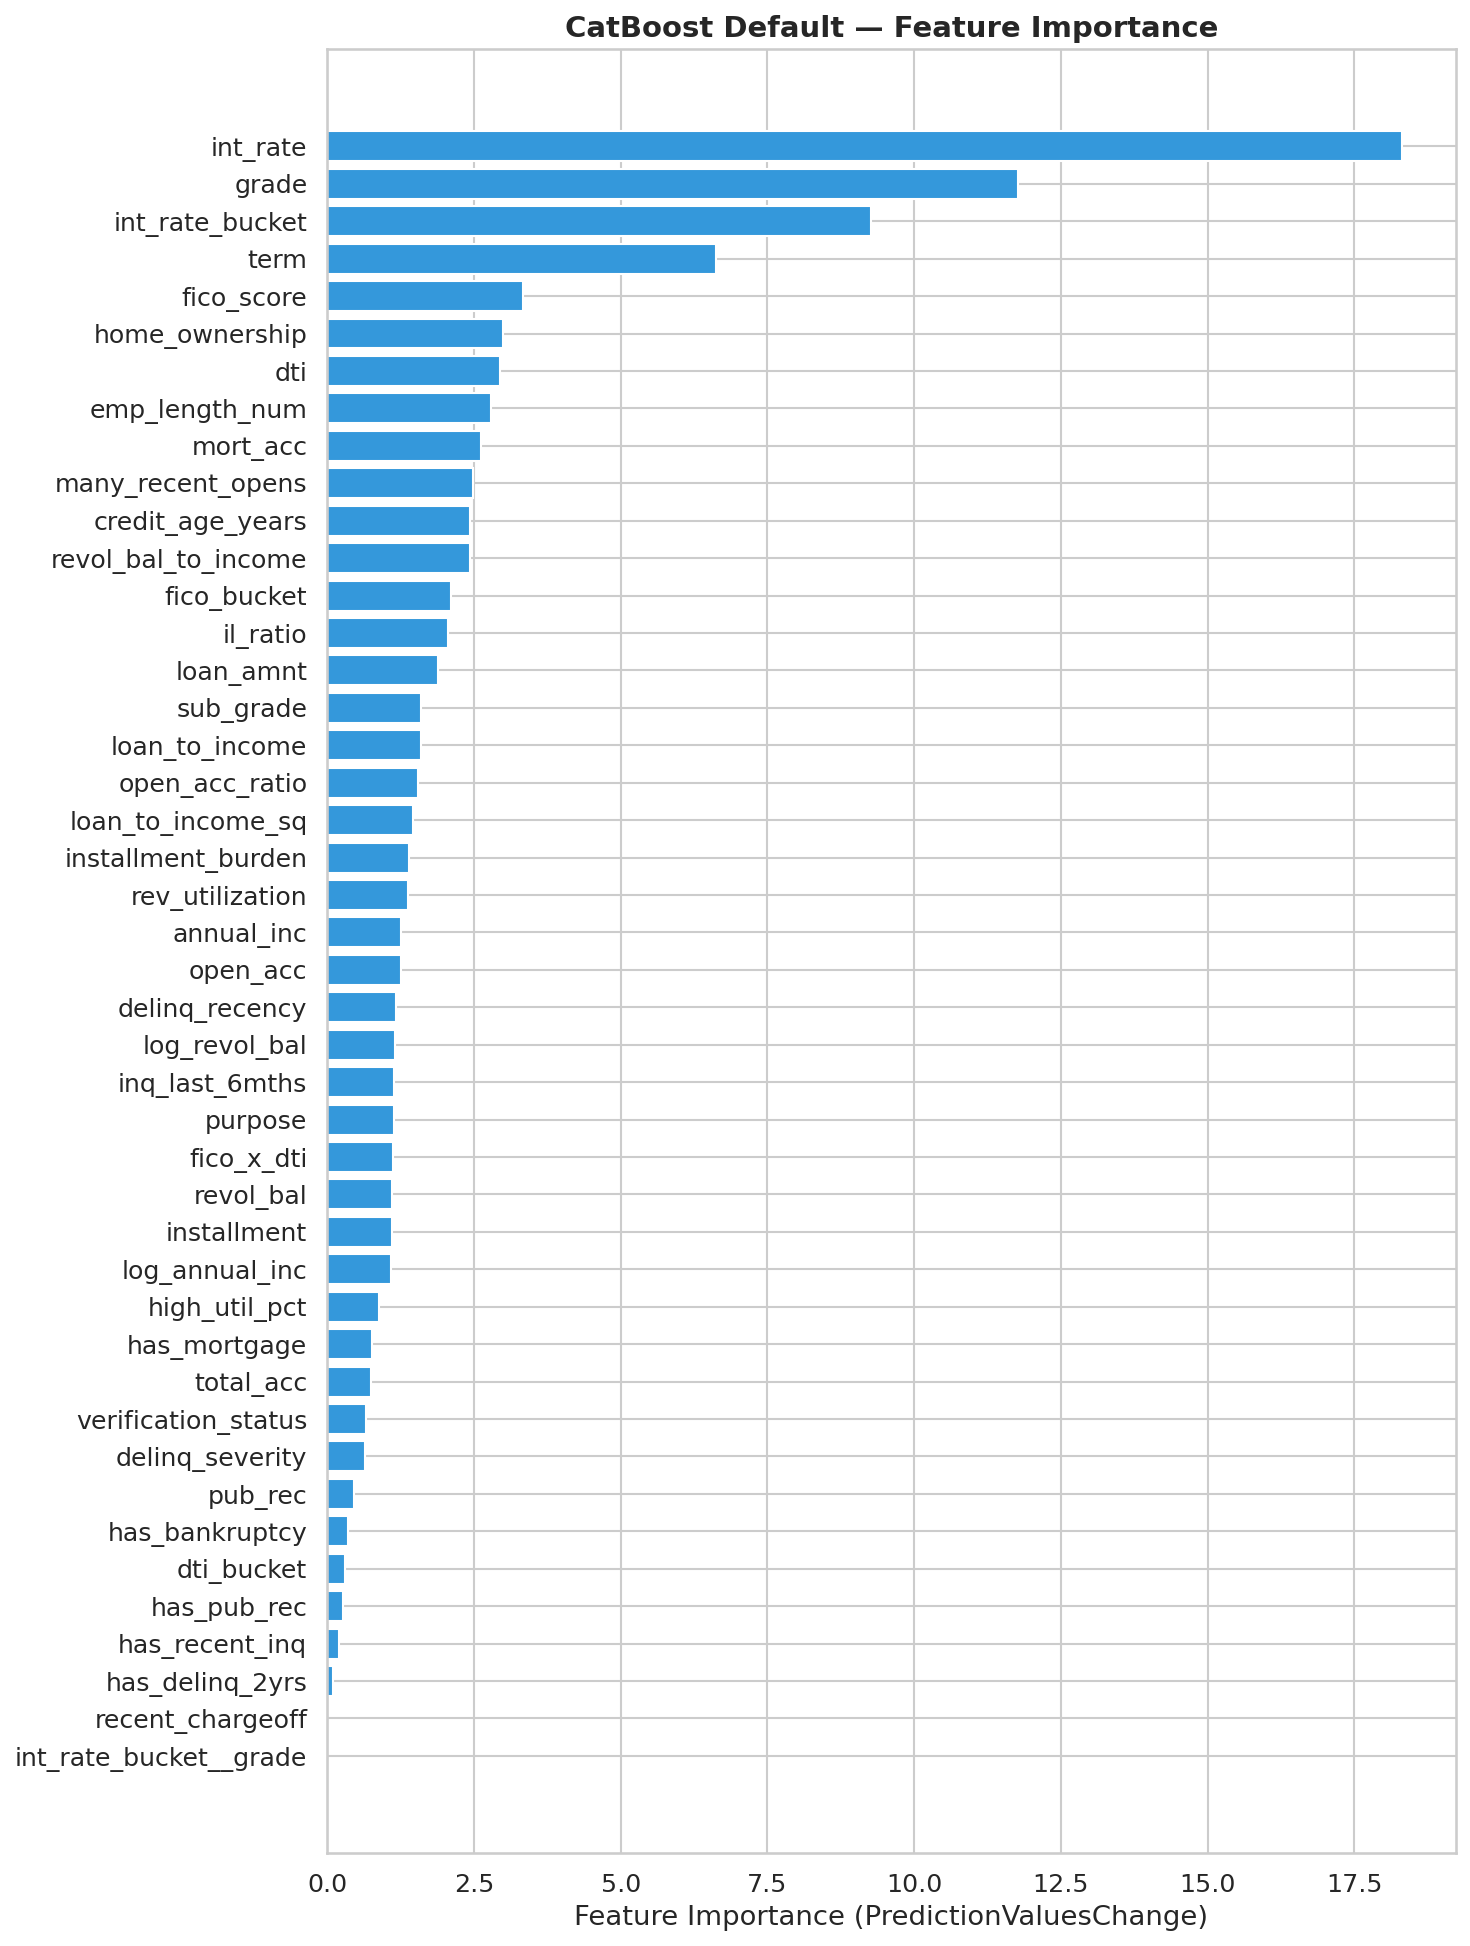
\includegraphics[keepaspectratio,alt={Importancia de variables del modelo champion de probabilidad de default.}]{chapters/06-pd-modeling/../../assets/figures/notebooks/feature_importance.png}}

}

\subcaption{Importancia agregada de variables del modelo PD champion,
como evidencia estática del bloque de modelado para exportación PDF.}

\end{figure}%

\end{minipage}%
%
\begin{minipage}[t]{0.50\linewidth}

\begin{figure}[H]

{\centering \pandocbounded{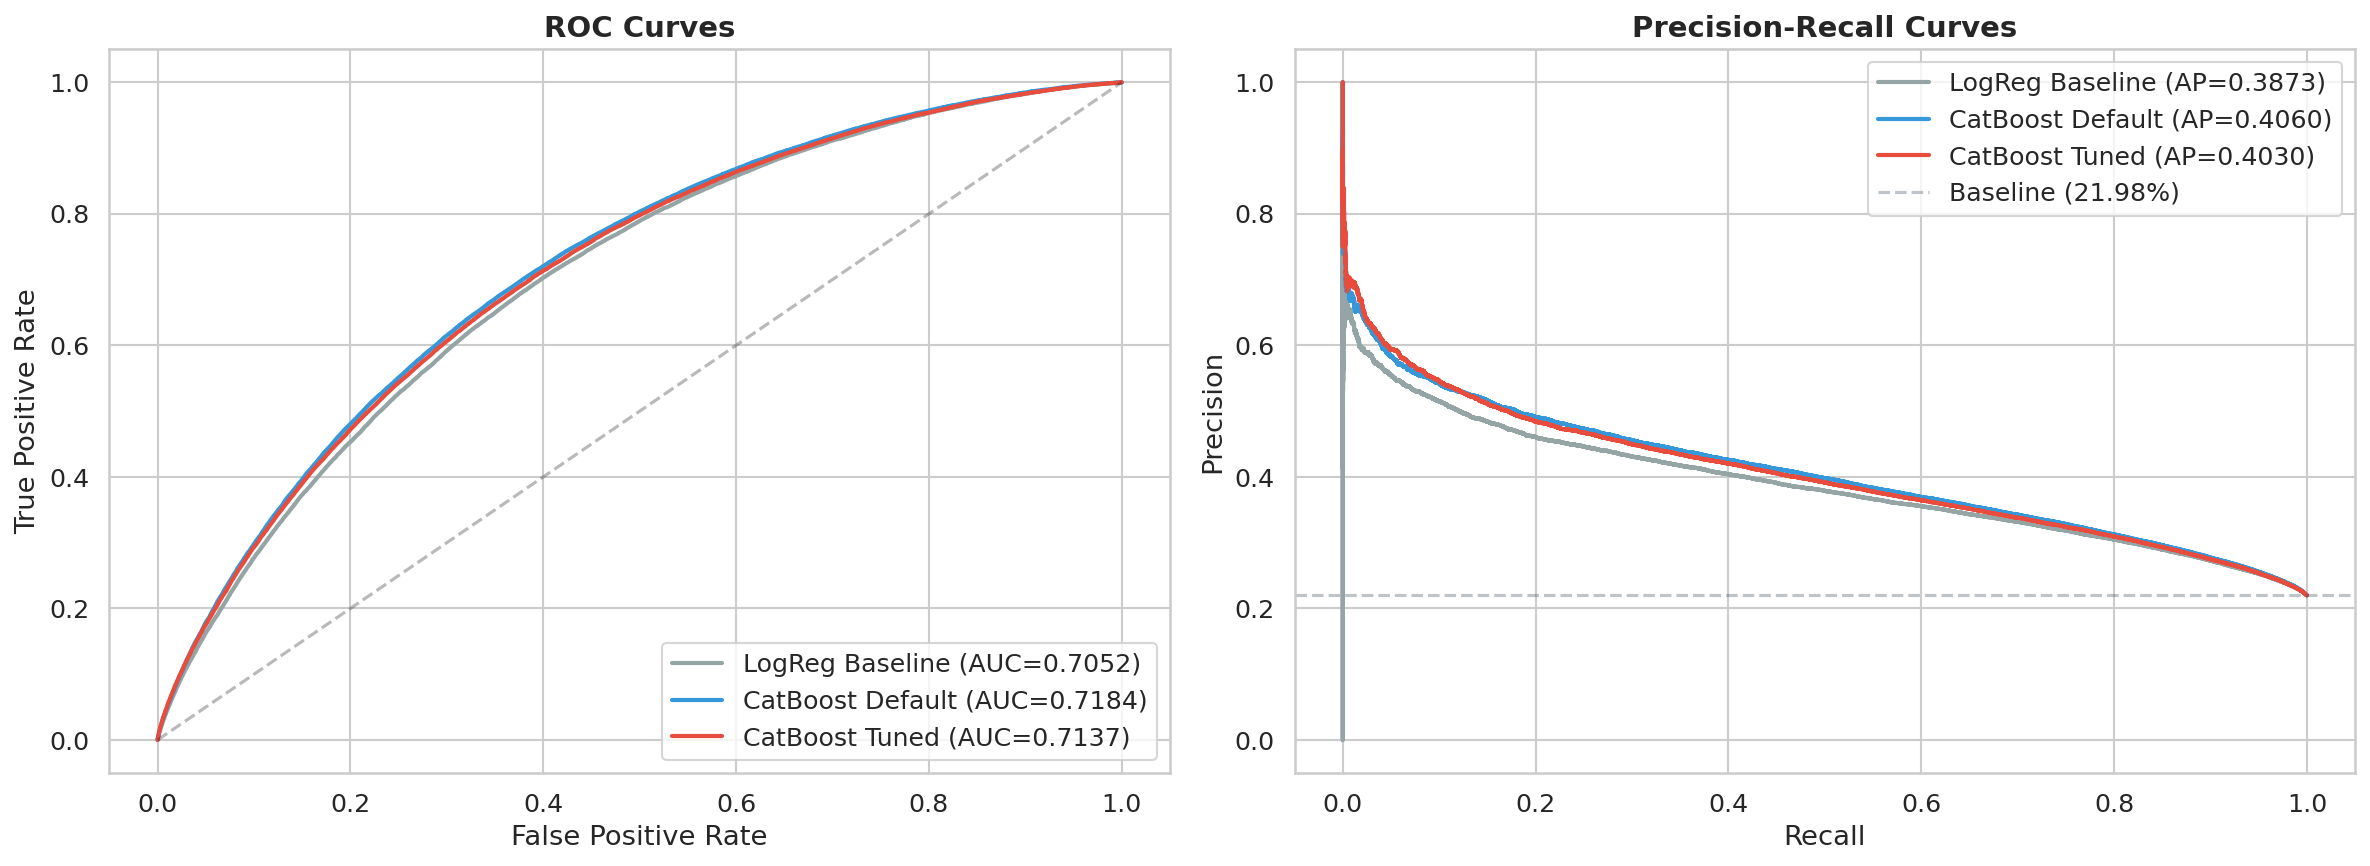
\includegraphics[keepaspectratio,alt={Curvas ROC comparando los modelos principales de probabilidad de default.}]{chapters/06-pd-modeling/../../assets/figures/notebooks/roc_curves.png}}

}

\subcaption{Curvas ROC de los modelos PD principales evaluados en el
proyecto.}

\end{figure}%

\end{minipage}%

\end{figure*}%

\begin{table}

\caption{\label{tbl-model-overview}Resumen de modelos PD evaluados}

\centering{

\begin{Shaded}
\begin{Highlighting}[]
\ImportTok{import}\NormalTok{ sys}
\ImportTok{from}\NormalTok{ pathlib }\ImportTok{import}\NormalTok{ Path}

\NormalTok{sys.path.insert(}\DecValTok{0}\NormalTok{, }\BuiltInTok{str}\NormalTok{(Path.cwd().parent }\ControlFlowTok{if}\NormalTok{ Path.cwd().name }\OperatorTok{==} \StringTok{"book"} \ControlFlowTok{else}\NormalTok{ Path.cwd()))}
\ImportTok{from}\NormalTok{ book.\_helpers.load\_artifacts }\ImportTok{import}\NormalTok{ load\_json}

\ImportTok{import}\NormalTok{ pandas }\ImportTok{as}\NormalTok{ pd}

\NormalTok{comparison }\OperatorTok{=}\NormalTok{ load\_json(}\StringTok{"model\_comparison"}\NormalTok{)}
\NormalTok{models }\OperatorTok{=}\NormalTok{ comparison.get(}\StringTok{"models"}\NormalTok{, [])}

\NormalTok{df\_models }\OperatorTok{=}\NormalTok{ pd.DataFrame(models)[[}\StringTok{"model"}\NormalTok{, }\StringTok{"calibrated"}\NormalTok{, }\StringTok{"auc"}\NormalTok{, }\StringTok{"gini"}\NormalTok{, }\StringTok{"brier"}\NormalTok{, }\StringTok{"d2\_brier"}\NormalTok{]]}
\NormalTok{df\_models.columns }\OperatorTok{=}\NormalTok{ [}\StringTok{"Modelo"}\NormalTok{, }\StringTok{"Calibrado"}\NormalTok{, }\StringTok{"AUC"}\NormalTok{, }\StringTok{"Gini"}\NormalTok{, }\StringTok{"Brier"}\NormalTok{, }\StringTok{"D² Brier"}\NormalTok{]}
\NormalTok{df\_models}
\end{Highlighting}
\end{Shaded}

}

\end{table}%

Cada modelo se evalúa exclusivamente sobre el set de test OOT
(2018--2020), nunca sobre datos de entrenamiento o validación. Las
métricas reflejan rendimiento prospectivo genuino.

\chapter{Regresión Logística: Baseline
Interpretable}\label{sec-lr-baseline}

\subsection{¿Por qué un Baseline
Lineal?}\label{por-quuxe9-un-baseline-lineal}

Toda investigación rigurosa en machine learning requiere un
\textbf{baseline simple} contra el cual medir el valor agregado de
modelos más complejos. En credit scoring, la regresión logística no es
solo un baseline académico --- es el \textbf{estándar regulatorio}: la
mayoría de los scorecards en producción bancaria global siguen siendo
regresiones logísticas, y los reguladores evalúan modelos de ML
comparándolos contra este benchmark.

El baseline de regresión logística cumple cuatro funciones en el
pipeline:

\begin{enumerate}
\def\labelenumi{\arabic{enumi}.}
\tightlist
\item
  \textbf{Benchmark de discriminación}: ¿CatBoost realmente supera a un
  modelo lineal, o la ganancia de AUC es marginal?
\item
  \textbf{Referencia de interpretabilidad}: Los coeficientes de la LR
  son directamente interpretables como odds ratios, proporcionando una
  narrativa que los reguladores entienden.
\item
  \textbf{Validación de features}: Si una feature tiene un coeficiente
  significativo en la LR, tiene poder predictivo real. Si CatBoost la
  usa pero la LR no, el efecto puede ser una interacción no lineal.
\item
  \textbf{Lower bound de rendimiento}: Cualquier modelo desplegado debe
  superar \emph{significativamente} a la LR para justificar la
  complejidad adicional.
\end{enumerate}

\subsection{Especificación del
Modelo}\label{especificaciuxf3n-del-modelo}

La regresión logística modela la probabilidad de default como:

\begin{equation}\protect\phantomsection\label{eq-logistic}{
P(\text{default} = 1 \mid \mathbf{x}) = \sigma(\mathbf{w}^\top \mathbf{x} + b) = \frac{1}{1 + e^{-(\mathbf{w}^\top \mathbf{x} + b)}}
}\end{equation}

donde \(\mathbf{w}\) son los pesos (uno por feature), \(b\) es el
intercepto, y \(\sigma(\cdot)\) es la función sigmoide.

\subsubsection{Preprocesamiento para LR}\label{preprocesamiento-para-lr}

A diferencia de CatBoost, la regresión logística requiere
preprocesamiento explícito:

\begin{longtable}[]{@{}
  >{\raggedright\arraybackslash}p{(\linewidth - 4\tabcolsep) * \real{0.2432}}
  >{\raggedright\arraybackslash}p{(\linewidth - 4\tabcolsep) * \real{0.3514}}
  >{\raggedright\arraybackslash}p{(\linewidth - 4\tabcolsep) * \real{0.4054}}@{}}
\caption{Preprocesamiento del baseline
LR}\label{tbl-lr-preprocessing}\tabularnewline
\toprule\noalign{}
\begin{minipage}[b]{\linewidth}\raggedright
Aspecto
\end{minipage} & \begin{minipage}[b]{\linewidth}\raggedright
Tratamiento
\end{minipage} & \begin{minipage}[b]{\linewidth}\raggedright
Justificación
\end{minipage} \\
\midrule\noalign{}
\endfirsthead
\toprule\noalign{}
\begin{minipage}[b]{\linewidth}\raggedright
Aspecto
\end{minipage} & \begin{minipage}[b]{\linewidth}\raggedright
Tratamiento
\end{minipage} & \begin{minipage}[b]{\linewidth}\raggedright
Justificación
\end{minipage} \\
\midrule\noalign{}
\endhead
\bottomrule\noalign{}
\endlastfoot
\textbf{NaN} & \texttt{fillna(0)} & Estrategia simple; LR no maneja NaN
nativamente \\
\textbf{Categorías} & WOE encoding & Las variables \texttt{\_woe} son
numéricas y monótonas \\
\textbf{Escala} & Sin estandarización & Los coeficientes se interpretan
en la escala original \\
\textbf{Regularización} & L2 por defecto (scikit-learn) & Previene
overfitting en features correlacionadas \\
\end{longtable}

\begin{tcolorbox}[enhanced jigsaw, arc=.35mm, bottomrule=.15mm, bottomtitle=1mm, breakable, colback=white, colbacktitle=quarto-callout-warning-color!10!white, colframe=quarto-callout-warning-color-frame, coltitle=black, left=2mm, leftrule=.75mm, opacityback=0, opacitybacktitle=0.6, rightrule=.15mm, title=\textcolor{quarto-callout-warning-color}{\faExclamationTriangle}\hspace{0.5em}{Limitación del fillna(0)}, titlerule=0mm, toprule=.15mm, toptitle=1mm]

Reemplazar NaN con cero es una estrategia subóptima porque introduce un
sesgo: un DTI faltante (que podría indicar datos incompletos o un
autoempleado) se trata igual que un DTI de cero (sin deuda). Para la LR
baseline, esta simplificación es aceptable porque el objetivo es
establecer un lower bound, no maximizar rendimiento. CatBoost no sufre
esta limitación al tratar NaN como un valor informativo propio.

\end{tcolorbox}

\subsection{Métricas del Baseline}\label{muxe9tricas-del-baseline}

\begin{table}

\caption{\label{tbl-lr-metrics}Métricas del baseline de Regresión
Logística (test OOT)}

\centering{

\begin{Shaded}
\begin{Highlighting}[]
\ImportTok{import}\NormalTok{ pandas }\ImportTok{as}\NormalTok{ pd}

\NormalTok{lr\_metrics }\OperatorTok{=}\NormalTok{ \{}
    \StringTok{"AUC{-}ROC"}\NormalTok{: }\StringTok{"0.683"}\NormalTok{,}
    \StringTok{"Gini"}\NormalTok{: }\StringTok{"0.366"}\NormalTok{,}
    \StringTok{"Brier Score (raw)"}\NormalTok{: }\StringTok{"0.2313"}\NormalTok{,}
    \StringTok{"D² Brier"}\NormalTok{: }\StringTok{"{-}0.349 (peor que naive)"}\NormalTok{,}
    \StringTok{"Interpretación AUC"}\NormalTok{: }\StringTok{"Discriminación aceptable pero limitada"}\NormalTok{,}
    \StringTok{"Gap vs CatBoost"}\NormalTok{: }\StringTok{"0.030 AUC (4.4}\SpecialCharTok{\% r}\StringTok{elativo)"}\NormalTok{,}
\NormalTok{\}}

\NormalTok{pd.DataFrame(}\BuiltInTok{list}\NormalTok{(lr\_metrics.items()), columns}\OperatorTok{=}\NormalTok{[}\StringTok{"Métrica"}\NormalTok{, }\StringTok{"Valor"}\NormalTok{])}
\end{Highlighting}
\end{Shaded}

}

\end{table}%

El AUC de 0.683 está en el rango típico para regresión logística
aplicada a credit scoring con datos de Lending Club. Estudios publicados
reportan AUC de 0.66--0.70 para modelos lineales sobre este dataset
({Lessmann et~al.}, 2015).

\begin{tcolorbox}[enhanced jigsaw, arc=.35mm, bottomrule=.15mm, bottomtitle=1mm, breakable, colback=white, colbacktitle=quarto-callout-note-color!10!white, colframe=quarto-callout-note-color-frame, coltitle=black, left=2mm, leftrule=.75mm, opacityback=0, opacitybacktitle=0.6, rightrule=.15mm, title=\textcolor{quarto-callout-note-color}{\faInfo}\hspace{0.5em}{D² Brier negativo: ¿qué significa?}, titlerule=0mm, toprule=.15mm, toptitle=1mm]

El D² Brier Score es análogo al R² --- mide la mejora relativa sobre un
predictor naive (que siempre predice la frecuencia marginal de default).
Un D² negativo (-0.349) indica que el Brier Score del modelo es
\textbf{peor} que el predictor naive. Esto no significa que la LR sea
inútil --- su AUC es 0.683, indicando buena discriminación. El problema
es la \textbf{calibración}: los scores brutos de la LR no son
probabilidades bien calibradas. Este es precisamente el problema que la
etapa de calibración post-hoc resuelve.

\end{tcolorbox}

\subsection{Valor del Baseline}\label{valor-del-baseline}

La comparación LR vs.~CatBoost justifica el uso de un modelo más
complejo:

\begin{itemize}
\tightlist
\item
  \textbf{AUC}: 0.683 → 0.713 (+0.030, +4.4\% relativo). Una mejora de 3
  puntos de AUC es considerada significativa en credit scoring aplicado.
\item
  \textbf{Gini}: 0.366 → 0.426 (+0.060). El Gini amplifica la
  diferencia.
\item
  \textbf{Brier}: 0.231 → 0.154 (después de calibración). Una reducción
  del 33\% en error cuadrático.
\end{itemize}

Estas mejoras justifican la complejidad adicional de CatBoost para un
modelo de producción, mientras que la LR queda como referencia
interpretable para auditoría regulatoria.

\chapter{CatBoost: Default y Optimizado con
Optuna}\label{sec-catboost-tuned}

\subsection{Arquitectura de CatBoost}\label{arquitectura-de-catboost}

CatBoost (\emph{Categorical Boosting}) es un algoritmo de gradient
boosting desarrollado por Yandex que introduce dos innovaciones
fundamentales respecto a sus competidores XGBoost y LightGBM:
\textbf{ordered boosting} y \textbf{arboles oblivious} (simétricos).

\subsubsection{Ordered Boosting}\label{ordered-boosting}

El gradient boosting estándar calcula los residuos sobre las mismas
observaciones usadas para construir los árboles anteriores, lo que
introduce un sesgo de \emph{target leakage} especialmente en datasets
pequeños. CatBoost resuelve esto con \emph{ordered boosting}: para cada
observación \(i\), los residuos se calculan usando un modelo entrenado
solo en observaciones anteriores a \(i\) (según una permutación
aleatoria del dataset). Formalmente, el residuo para la observación
\(i\) en la iteración \(t\) es:

\begin{equation}\protect\phantomsection\label{eq-ordered-boosting}{
r_i^{(t)} = y_i - \hat{f}^{(t-1)}_{\sigma_{<i}}(x_i)
}\end{equation}

donde \(\hat{f}^{(t-1)}_{\sigma_{<i}}\) es el modelo construido
únicamente con las observaciones que preceden a \(i\) en la permutación
\(\sigma\). Esto produce estimaciones de gradiente insesgadas a cambio
de mayor costo computacional.

\subsubsection{Arboles Oblivious
(Simétricos)}\label{arboles-oblivious-simuxe9tricos}

CatBoost utiliza por defecto \emph{oblivious decision trees} (ODT),
donde cada nivel del árbol usa la \textbf{misma condición de split} para
todos los nodos de ese nivel. Esto significa que un árbol de profundidad
\(d\) tiene exactamente \(2^d\) hojas, y la estructura se puede
representar como una tabla de verdad de \(d\) condiciones binarias.

Las ventajas para credit scoring son:

\begin{itemize}
\tightlist
\item
  \textbf{Regularización implícita}: la simetría reduce drásticamente el
  número de parámetros libres, previniendo overfitting.
\item
  \textbf{Velocidad de inferencia}: la predicción se resuelve como una
  tabla de lookup, no como una travesía del árbol.
\item
  \textbf{Estabilidad}: modelos entrenados con semillas diferentes
  producen predicciones más similares entre sí.
\end{itemize}

\subsubsection{Manejo Nativo de Categorías y
NaN}\label{manejo-nativo-de-categoruxedas-y-nan}

CatBoost procesa variables categóricas sin necesidad de one-hot encoding
o WOE, usando \emph{target statistics} con suavizado:

\begin{equation}\protect\phantomsection\label{eq-target-statistics}{
\hat{x}_k^i = \frac{\sum_{j \in \sigma_{<i}} \mathbb{1}[x_j^k = x_i^k] \cdot y_j + a \cdot p}{\sum_{j \in \sigma_{<i}} \mathbb{1}[x_j^k = x_i^k] + a}
}\end{equation}

donde \(p\) es la media global del target, \(a\) es un parámetro de
suavizado, y \(\sigma_{<i}\) es el conjunto de observaciones anteriores
en la permutación. Este esquema evita el target leakage que afecta al
encoding naive de medias condicionales.

Para valores faltantes (NaN), CatBoost asigna cada observación con NaN a
la rama óptima en cada split --- izquierda o derecha --- maximizando la
métrica objetivo. Esto convierte la ausencia de datos en una señal
informativa sin requerir imputación manual.

\subsection{Ventajas sobre XGBoost/LightGBM para Credit
Scoring}\label{sec-catboost-advantages}

La selección de CatBoost como modelo principal no es arbitraria. Para
aplicaciones de credit scoring, presenta ventajas concretas:

\begin{longtable}[]{@{}
  >{\raggedright\arraybackslash}p{(\linewidth - 6\tabcolsep) * \real{0.2368}}
  >{\raggedright\arraybackslash}p{(\linewidth - 6\tabcolsep) * \real{0.2632}}
  >{\raggedright\arraybackslash}p{(\linewidth - 6\tabcolsep) * \real{0.2368}}
  >{\raggedright\arraybackslash}p{(\linewidth - 6\tabcolsep) * \real{0.2632}}@{}}
\caption{Comparación de frameworks de gradient boosting para credit
scoring}\label{tbl-catboost-vs-others}\tabularnewline
\toprule\noalign{}
\begin{minipage}[b]{\linewidth}\raggedright
Aspecto
\end{minipage} & \begin{minipage}[b]{\linewidth}\raggedright
CatBoost
\end{minipage} & \begin{minipage}[b]{\linewidth}\raggedright
XGBoost
\end{minipage} & \begin{minipage}[b]{\linewidth}\raggedright
LightGBM
\end{minipage} \\
\midrule\noalign{}
\endfirsthead
\toprule\noalign{}
\begin{minipage}[b]{\linewidth}\raggedright
Aspecto
\end{minipage} & \begin{minipage}[b]{\linewidth}\raggedright
CatBoost
\end{minipage} & \begin{minipage}[b]{\linewidth}\raggedright
XGBoost
\end{minipage} & \begin{minipage}[b]{\linewidth}\raggedright
LightGBM
\end{minipage} \\
\midrule\noalign{}
\endhead
\bottomrule\noalign{}
\endlastfoot
\textbf{Categorías} & Nativo (target statistics) & Requiere encoding
manual & Nativo (split por subconjuntos) \\
\textbf{NaN} & Nativo (optimal branch) & Nativo (default direction) &
Nativo (zero bin) \\
\textbf{Calibración} & Mejor out-of-box & Requiere post-hoc & Requiere
post-hoc \\
\textbf{Sensibilidad a HPO} & Baja (defaults robustos) & Media-alta &
Alta \\
\textbf{Arboles} & Oblivious (regularizados) & Asimétricos & Asimétricos
(leaf-wise) \\
\textbf{Ordered boosting} & Si & No & No \\
\end{longtable}

\begin{tcolorbox}[enhanced jigsaw, arc=.35mm, bottomrule=.15mm, bottomtitle=1mm, breakable, colback=white, colbacktitle=quarto-callout-tip-color!10!white, colframe=quarto-callout-tip-color-frame, coltitle=black, left=2mm, leftrule=.75mm, opacityback=0, opacitybacktitle=0.6, rightrule=.15mm, title=\textcolor{quarto-callout-tip-color}{\faLightbulb}\hspace{0.5em}{Calibración out-of-box}, titlerule=0mm, toprule=.15mm, toptitle=1mm]

La combinación de ordered boosting y árboles oblivious produce
predicciones que son \emph{a priori} mejor calibradas que las de
XGBoost/LightGBM. Esto es relevante en credit scoring, donde las
probabilidades no solo deben ordenar bien a los clientes
(discriminación), sino reflejar la tasa de default real (calibración).
Aun así, la calibración post-hoc es necesaria para uso regulatorio ---
ver Capítulo~\ref{sec-calibration-selection}.

\end{tcolorbox}

\subsection{CatBoost Default}\label{sec-catboost-default}

El primer modelo CatBoost se entrena con hiperparámetros base
conservadores, heredados del estándar de scikit-learn adaptado a la
escala del dataset:

\begin{table}

\caption{\label{tbl-catboost-default-params}Hiperparámetros del CatBoost
default}

\centering{

\begin{Shaded}
\begin{Highlighting}[]
\ImportTok{import}\NormalTok{ sys}
\ImportTok{from}\NormalTok{ pathlib }\ImportTok{import}\NormalTok{ Path}

\NormalTok{sys.path.insert(}\DecValTok{0}\NormalTok{, }\BuiltInTok{str}\NormalTok{(Path.cwd().parent }\ControlFlowTok{if}\NormalTok{ Path.cwd().name }\OperatorTok{==} \StringTok{"book"} \ControlFlowTok{else}\NormalTok{ Path.cwd()))}

\ImportTok{import}\NormalTok{ pandas }\ImportTok{as}\NormalTok{ pd}

\NormalTok{default\_params }\OperatorTok{=}\NormalTok{ \{}
    \StringTok{"iterations"}\NormalTok{: }\StringTok{"1,000"}\NormalTok{,}
    \StringTok{"learning\_rate"}\NormalTok{: }\StringTok{"0.05"}\NormalTok{,}
    \StringTok{"depth"}\NormalTok{: }\StringTok{"6"}\NormalTok{,}
    \StringTok{"l2\_leaf\_reg"}\NormalTok{: }\StringTok{"3.0"}\NormalTok{,}
    \StringTok{"loss\_function"}\NormalTok{: }\StringTok{"Logloss"}\NormalTok{,}
    \StringTok{"auto\_class\_weights"}\NormalTok{: }\StringTok{"Balanced"}\NormalTok{,}
    \StringTok{"eval\_metric"}\NormalTok{: }\StringTok{"AUC"}\NormalTok{,}
    \StringTok{"early\_stopping\_rounds"}\NormalTok{: }\StringTok{"50"}\NormalTok{,}
    \StringTok{"has\_time"}\NormalTok{: }\StringTok{"True"}\NormalTok{,}
\NormalTok{\}}

\NormalTok{df\_params }\OperatorTok{=}\NormalTok{ pd.DataFrame(}
    \BuiltInTok{list}\NormalTok{(default\_params.items()),}
\NormalTok{    columns}\OperatorTok{=}\NormalTok{[}\StringTok{"Hiperparámetro"}\NormalTok{, }\StringTok{"Valor"}\NormalTok{],}
\NormalTok{)}
\NormalTok{df\_params}
\end{Highlighting}
\end{Shaded}

}

\end{table}%

El parámetro \texttt{has\_time=True} indica a CatBoost que el orden de
las observaciones es informativo (temporal), lo cual ajusta las
permutaciones del ordered boosting para respetar la estructura temporal
--- un detalle importante para datos de crédito donde la distribución
cambia con el ciclo económico.

El entrenamiento utiliza un split temporal donde el 15\% final del set
de entrenamiento sirve como validación para early stopping, garantizando
que la selección de la mejor iteración es prospectiva.

\begin{table}

\caption{\label{tbl-catboost-default-metrics}Métricas del CatBoost
default (test OOT)}

\centering{

\begin{Shaded}
\begin{Highlighting}[]
\ImportTok{from}\NormalTok{ book.\_helpers.load\_artifacts }\ImportTok{import}\NormalTok{ load\_json}

\NormalTok{comparison }\OperatorTok{=}\NormalTok{ load\_json(}\StringTok{"model\_comparison"}\NormalTok{)}
\NormalTok{models }\OperatorTok{=}\NormalTok{ comparison.get(}\StringTok{"models"}\NormalTok{, [])}

\CommentTok{\# Extraer métricas del modelo default}
\NormalTok{cb\_default }\OperatorTok{=} \BuiltInTok{next}\NormalTok{((m }\ControlFlowTok{for}\NormalTok{ m }\KeywordTok{in}\NormalTok{ models }\ControlFlowTok{if}\NormalTok{ m[}\StringTok{"model"}\NormalTok{] }\OperatorTok{==} \StringTok{"CatBoost (default)"}\NormalTok{), }\VariableTok{None}\NormalTok{)}

\ControlFlowTok{if}\NormalTok{ cb\_default:}
\NormalTok{    metrics\_default }\OperatorTok{=}\NormalTok{ \{}
        \StringTok{"AUC{-}ROC"}\NormalTok{: }\SpecialStringTok{f"}\SpecialCharTok{\{}\NormalTok{cb\_default[}\StringTok{\textquotesingle{}auc\textquotesingle{}}\NormalTok{]}\SpecialCharTok{:.4f\}}\SpecialStringTok{"}\NormalTok{,}
        \StringTok{"Gini"}\NormalTok{: }\SpecialStringTok{f"}\SpecialCharTok{\{}\NormalTok{cb\_default[}\StringTok{\textquotesingle{}gini\textquotesingle{}}\NormalTok{]}\SpecialCharTok{:.3f\}}\SpecialStringTok{"}\NormalTok{,}
        \StringTok{"Brier Score (raw)"}\NormalTok{: }\SpecialStringTok{f"}\SpecialCharTok{\{}\NormalTok{cb\_default[}\StringTok{\textquotesingle{}brier\textquotesingle{}}\NormalTok{]}\SpecialCharTok{:.4f\}}\SpecialStringTok{"}\NormalTok{,}
        \StringTok{"D² Brier"}\NormalTok{: }\SpecialStringTok{f"}\SpecialCharTok{\{}\NormalTok{cb\_default[}\StringTok{\textquotesingle{}d2\_brier\textquotesingle{}}\NormalTok{]}\SpecialCharTok{:.4f\}}\SpecialStringTok{"}\NormalTok{,}
        \StringTok{"Gap vs LR baseline"}\NormalTok{: }\SpecialStringTok{f"+}\SpecialCharTok{\{}\NormalTok{cb\_default[}\StringTok{\textquotesingle{}auc\textquotesingle{}}\NormalTok{] }\OperatorTok{{-}} \FloatTok{0.683}\SpecialCharTok{:.4f\}}\SpecialStringTok{ AUC (+}\SpecialCharTok{\{}\NormalTok{(cb\_default[}\StringTok{\textquotesingle{}auc\textquotesingle{}}\NormalTok{] }\OperatorTok{{-}} \FloatTok{0.683}\NormalTok{)}\OperatorTok{/}\FloatTok{0.683}\OperatorTok{*}\DecValTok{100}\SpecialCharTok{:.1f\}}\SpecialStringTok{\% relativo)"}\NormalTok{,}
\NormalTok{    \}}
\NormalTok{    pd.DataFrame(}\BuiltInTok{list}\NormalTok{(metrics\_default.items()), columns}\OperatorTok{=}\NormalTok{[}\StringTok{"Métrica"}\NormalTok{, }\StringTok{"Valor"}\NormalTok{])}
\end{Highlighting}
\end{Shaded}

}

\end{table}%

Con un AUC de 0.7125, el CatBoost default ya supera sustancialmente a la
LR baseline (0.683, ver Capítulo~\ref{sec-lr-baseline}), demostrando que
las interacciones no lineales y el procesamiento nativo de categorías
aportan +0.030 AUC (+4.3\% relativo). La pregunta es si la optimización
de hiperparámetros puede mejorar aún más este rendimiento.

\subsection{Optimización con Optuna (HPO)}\label{sec-optuna-hpo}

\subsubsection{Diseño del Experimento}\label{diseuxf1o-del-experimento}

La optimización de hiperparámetros se ejecuta con Optuna, un framework
de HPO que implementa el \textbf{Tree-structured Parzen Estimator} (TPE)
como sampler por defecto. A diferencia de grid search o random search,
TPE modela la distribución de hiperparámetros condicionalmente al
rendimiento observado:

\begin{equation}\protect\phantomsection\label{eq-tpe}{
p(\lambda \mid y) = \frac{p(y \mid \lambda) \, p(\lambda)}{p(y)} \propto \begin{cases} \ell(\lambda) & \text{si } y < y^* \\ g(\lambda) & \text{si } y \geq y^* \end{cases}
}\end{equation}

donde \(y^*\) es el cuantil \(\gamma\) de los valores observados,
\(\ell(\lambda)\) modela la densidad de los hiperparámetros que
produjeron buenos resultados, y \(g(\lambda)\) modela los que produjeron
malos resultados. TPE maximiza el ratio \(\ell(\lambda)/g(\lambda)\), lo
cual es equivalente a maximizar el \emph{Expected Improvement} (EI).

La configuración de Optuna incluye además:

\begin{itemize}
\tightlist
\item
  \textbf{TPE multivariado con agrupación} (\texttt{multivariate=True},
  \texttt{group=True}): modela las dependencias entre hiperparámetros en
  lugar de tratarlos como independientes. Esto captura interacciones
  importantes como la relación entre \texttt{depth} y
  \texttt{learning\_rate}.
\item
  \textbf{MedianPruner}: detiene tempranamente trials que a la iteración
  \(t\) del boosting tienen AUC inferior a la mediana de los trials
  completados, ahorrando entre 40--60\% del cómputo total.
\item
  \textbf{Estudio persistente en SQLite}: permite retomar la búsqueda en
  sesiones posteriores sin perder el historial de trials.
\end{itemize}

\subsubsection{Espacio de Búsqueda}\label{espacio-de-buxfasqueda}

\begin{table}

\caption{\label{tbl-search-space}Espacio de búsqueda de Optuna para
CatBoost}

\centering{

\begin{Shaded}
\begin{Highlighting}[]
\NormalTok{search\_space }\OperatorTok{=}\NormalTok{ \{}
    \StringTok{"learning\_rate"}\NormalTok{: }\StringTok{"LogUniform(0.005, 0.20)"}\NormalTok{,}
    \StringTok{"depth"}\NormalTok{: }\StringTok{"Int(4, 10)"}\NormalTok{,}
    \StringTok{"l2\_leaf\_reg"}\NormalTok{: }\StringTok{"LogUniform(0.5, 100.0)"}\NormalTok{,}
    \StringTok{"min\_data\_in\_leaf"}\NormalTok{: }\StringTok{"Int(20, 500)"}\NormalTok{,}
    \StringTok{"random\_strength"}\NormalTok{: }\StringTok{"LogUniform(1e{-}9, 10.0)"}\NormalTok{,}
    \StringTok{"border\_count"}\NormalTok{: }\StringTok{"Int(64, 254)"}\NormalTok{,}
    \StringTok{"rsm (column sampling)"}\NormalTok{: }\StringTok{"Uniform(0.5, 1.0)"}\NormalTok{,}
    \StringTok{"bootstrap\_type"}\NormalTok{: }\StringTok{"Categorical(Bayesian, Bernoulli, MVS)"}\NormalTok{,}
    \StringTok{"grow\_policy"}\NormalTok{: }\StringTok{"Categorical(SymmetricTree, Depthwise, Lossguide)"}\NormalTok{,}
    \StringTok{"subsample*"}\NormalTok{: }\StringTok{"Uniform(0.5, 0.95)"}\NormalTok{,}
    \StringTok{"bagging\_temperature*"}\NormalTok{: }\StringTok{"Uniform(0.0, 10.0)"}\NormalTok{,}
    \StringTok{"leaf\_estimation\_iterations"}\NormalTok{: }\StringTok{"Int(1, 10)"}\NormalTok{,}
\NormalTok{\}}

\NormalTok{pd.DataFrame(}
    \BuiltInTok{list}\NormalTok{(search\_space.items()),}
\NormalTok{    columns}\OperatorTok{=}\NormalTok{[}\StringTok{"Hiperparámetro"}\NormalTok{, }\StringTok{"Distribución"}\NormalTok{],}
\NormalTok{)}
\end{Highlighting}
\end{Shaded}

}

\end{table}%

\emph{* \texttt{subsample} se aplica cuando \texttt{bootstrap\_type} es
Bernoulli o MVS; \texttt{bagging\_temperature} se aplica cuando es
Bayesian. Optuna maneja esta condicionalidad automáticamente.}

El espacio de búsqueda está diseñado para explorar tres familias de
regularización simultáneamente:

\begin{enumerate}
\def\labelenumi{\arabic{enumi}.}
\tightlist
\item
  \textbf{Regularización del árbol}: \texttt{depth},
  \texttt{min\_data\_in\_leaf}, \texttt{grow\_policy}
\item
  \textbf{Regularización del gradiente}: \texttt{learning\_rate},
  \texttt{l2\_leaf\_reg}, \texttt{random\_strength}
\item
  \textbf{Regularización por submuestreo}: \texttt{bootstrap\_type},
  \texttt{subsample}/\texttt{bagging\_temperature}, \texttt{rsm}
\end{enumerate}

\subsubsection{Resultados de la
Búsqueda}\label{resultados-de-la-buxfasqueda}

\begin{table}

\caption{\label{tbl-optuna-results}Resultados de la optimización con
Optuna}

\centering{

\begin{Shaded}
\begin{Highlighting}[]
\NormalTok{n\_trials }\OperatorTok{=}\NormalTok{ comparison.get(}\StringTok{"hpo\_trials\_executed"}\NormalTok{, }\DecValTok{320}\NormalTok{)}
\NormalTok{best\_val\_auc }\OperatorTok{=}\NormalTok{ comparison.get(}\StringTok{"hpo\_best\_validation\_auc"}\NormalTok{, }\FloatTok{0.7227}\NormalTok{)}
\NormalTok{cb\_tuned }\OperatorTok{=} \BuiltInTok{next}\NormalTok{((m }\ControlFlowTok{for}\NormalTok{ m }\KeywordTok{in}\NormalTok{ models }\ControlFlowTok{if}\NormalTok{ m[}\StringTok{"model"}\NormalTok{] }\OperatorTok{==} \StringTok{"CatBoost (tuned)"}\NormalTok{), }\VariableTok{None}\NormalTok{)}

\NormalTok{optuna\_results }\OperatorTok{=}\NormalTok{ \{}
    \StringTok{"Trials ejecutados"}\NormalTok{: }\SpecialStringTok{f"}\SpecialCharTok{\{}\NormalTok{n\_trials}\SpecialCharTok{:,\}}\SpecialStringTok{"}\NormalTok{,}
    \StringTok{"Mejor AUC validación"}\NormalTok{: }\SpecialStringTok{f"}\SpecialCharTok{\{}\NormalTok{best\_val\_auc}\SpecialCharTok{:.4f\}}\SpecialStringTok{"}\NormalTok{,}
    \StringTok{"AUC test OOT (tuned)"}\NormalTok{: }\SpecialStringTok{f"}\SpecialCharTok{\{}\NormalTok{cb\_tuned[}\StringTok{\textquotesingle{}auc\textquotesingle{}}\NormalTok{]}\SpecialCharTok{:.4f\}}\SpecialStringTok{"} \ControlFlowTok{if}\NormalTok{ cb\_tuned }\ControlFlowTok{else} \StringTok{"N/A"}\NormalTok{,}
    \StringTok{"AUC test OOT (default)"}\NormalTok{: }\SpecialStringTok{f"}\SpecialCharTok{\{}\NormalTok{cb\_default[}\StringTok{\textquotesingle{}auc\textquotesingle{}}\NormalTok{]}\SpecialCharTok{:.4f\}}\SpecialStringTok{"} \ControlFlowTok{if}\NormalTok{ cb\_default }\ControlFlowTok{else} \StringTok{"N/A"}\NormalTok{,}
    \StringTok{"Mejora absoluta"}\NormalTok{: }\SpecialStringTok{f"+}\SpecialCharTok{\{}\NormalTok{cb\_tuned[}\StringTok{\textquotesingle{}auc\textquotesingle{}}\NormalTok{] }\OperatorTok{{-}}\NormalTok{ cb\_default[}\StringTok{\textquotesingle{}auc\textquotesingle{}}\NormalTok{]}\SpecialCharTok{:.4f\}}\SpecialStringTok{"} \ControlFlowTok{if}\NormalTok{ cb\_tuned }\KeywordTok{and}\NormalTok{ cb\_default }\ControlFlowTok{else} \StringTok{"N/A"}\NormalTok{,}
    \StringTok{"Sampler"}\NormalTok{: }\StringTok{"TPE multivariado con agrupación"}\NormalTok{,}
    \StringTok{"Pruner"}\NormalTok{: }\StringTok{"MedianPruner (n\_warmup=120)"}\NormalTok{,}
\NormalTok{\}}

\NormalTok{pd.DataFrame(}\BuiltInTok{list}\NormalTok{(optuna\_results.items()), columns}\OperatorTok{=}\NormalTok{[}\StringTok{"Aspecto"}\NormalTok{, }\StringTok{"Valor"}\NormalTok{])}
\end{Highlighting}
\end{Shaded}

}

\end{table}%

Los 320 trials alcanzaron un AUC de validación de 0.7227, pero el AUC en
el test OOT es 0.7131 --- una brecha de 0.0096 que indica \emph{temporal
overfitting} al set de validación. El set de validación temporal cubre
un período específico (cola del período 2007--2017), mientras que el
test OOT abarca 2018--2020 con condiciones macroeconómicas
potencialmente diferentes.

\subsubsection{Hiperparámetros
Ganadores}\label{hiperparuxe1metros-ganadores}

\begin{table}

\caption{\label{tbl-best-params}Hiperparámetros óptimos seleccionados
por Optuna}

\centering{

\begin{Shaded}
\begin{Highlighting}[]
\ImportTok{from}\NormalTok{ book.\_helpers.load\_artifacts }\ImportTok{import}\NormalTok{ load\_yaml}

\NormalTok{config }\OperatorTok{=}\NormalTok{ load\_yaml(}\StringTok{"pd\_model"}\NormalTok{)}
\NormalTok{tuned\_params }\OperatorTok{=}\NormalTok{ config.get(}\StringTok{"model"}\NormalTok{, \{\}).get(}\StringTok{"params"}\NormalTok{, \{\})}

\CommentTok{\# Mostrar los parámetros más relevantes}
\NormalTok{key\_params }\OperatorTok{=}\NormalTok{ \{}
    \StringTok{"iterations"}\NormalTok{: tuned\_params.get(}\StringTok{"iterations"}\NormalTok{, }\StringTok{"N/A"}\NormalTok{),}
    \StringTok{"learning\_rate"}\NormalTok{: }\SpecialStringTok{f"}\SpecialCharTok{\{}\NormalTok{tuned\_params}\SpecialCharTok{.}\NormalTok{get(}\StringTok{\textquotesingle{}learning\_rate\textquotesingle{}}\NormalTok{, }\StringTok{\textquotesingle{}N/A\textquotesingle{}}\NormalTok{)}\SpecialCharTok{:.4f\}}\SpecialStringTok{"} \ControlFlowTok{if} \BuiltInTok{isinstance}\NormalTok{(tuned\_params.get(}\StringTok{\textquotesingle{}learning\_rate\textquotesingle{}}\NormalTok{), (}\BuiltInTok{int}\NormalTok{, }\BuiltInTok{float}\NormalTok{)) }\ControlFlowTok{else} \StringTok{"N/A"}\NormalTok{,}
    \StringTok{"depth"}\NormalTok{: tuned\_params.get(}\StringTok{"depth"}\NormalTok{, }\StringTok{"N/A"}\NormalTok{),}
    \StringTok{"l2\_leaf\_reg"}\NormalTok{: }\SpecialStringTok{f"}\SpecialCharTok{\{}\NormalTok{tuned\_params}\SpecialCharTok{.}\NormalTok{get(}\StringTok{\textquotesingle{}l2\_leaf\_reg\textquotesingle{}}\NormalTok{, }\StringTok{\textquotesingle{}N/A\textquotesingle{}}\NormalTok{)}\SpecialCharTok{:.2f\}}\SpecialStringTok{"} \ControlFlowTok{if} \BuiltInTok{isinstance}\NormalTok{(tuned\_params.get(}\StringTok{\textquotesingle{}l2\_leaf\_reg\textquotesingle{}}\NormalTok{), (}\BuiltInTok{int}\NormalTok{, }\BuiltInTok{float}\NormalTok{)) }\ControlFlowTok{else} \StringTok{"N/A"}\NormalTok{,}
    \StringTok{"min\_data\_in\_leaf"}\NormalTok{: tuned\_params.get(}\StringTok{"min\_data\_in\_leaf"}\NormalTok{, }\StringTok{"N/A"}\NormalTok{),}
    \StringTok{"border\_count"}\NormalTok{: tuned\_params.get(}\StringTok{"border\_count"}\NormalTok{, }\StringTok{"N/A"}\NormalTok{),}
    \StringTok{"bootstrap\_type"}\NormalTok{: tuned\_params.get(}\StringTok{"bootstrap\_type"}\NormalTok{, }\StringTok{"N/A"}\NormalTok{),}
    \StringTok{"subsample"}\NormalTok{: }\SpecialStringTok{f"}\SpecialCharTok{\{}\NormalTok{tuned\_params}\SpecialCharTok{.}\NormalTok{get(}\StringTok{\textquotesingle{}subsample\textquotesingle{}}\NormalTok{, }\StringTok{\textquotesingle{}N/A\textquotesingle{}}\NormalTok{)}\SpecialCharTok{:.4f\}}\SpecialStringTok{"} \ControlFlowTok{if} \BuiltInTok{isinstance}\NormalTok{(tuned\_params.get(}\StringTok{\textquotesingle{}subsample\textquotesingle{}}\NormalTok{), (}\BuiltInTok{int}\NormalTok{, }\BuiltInTok{float}\NormalTok{)) }\ControlFlowTok{else} \StringTok{"N/A"}\NormalTok{,}
    \StringTok{"rsm"}\NormalTok{: }\SpecialStringTok{f"}\SpecialCharTok{\{}\NormalTok{tuned\_params}\SpecialCharTok{.}\NormalTok{get(}\StringTok{\textquotesingle{}rsm\textquotesingle{}}\NormalTok{, }\StringTok{\textquotesingle{}N/A\textquotesingle{}}\NormalTok{)}\SpecialCharTok{:.4f\}}\SpecialStringTok{"} \ControlFlowTok{if} \BuiltInTok{isinstance}\NormalTok{(tuned\_params.get(}\StringTok{\textquotesingle{}rsm\textquotesingle{}}\NormalTok{), (}\BuiltInTok{int}\NormalTok{, }\BuiltInTok{float}\NormalTok{)) }\ControlFlowTok{else} \StringTok{"N/A"}\NormalTok{,}
    \StringTok{"random\_strength"}\NormalTok{: }\SpecialStringTok{f"}\SpecialCharTok{\{}\NormalTok{tuned\_params}\SpecialCharTok{.}\NormalTok{get(}\StringTok{\textquotesingle{}random\_strength\textquotesingle{}}\NormalTok{, }\StringTok{\textquotesingle{}N/A\textquotesingle{}}\NormalTok{)}\SpecialCharTok{:.2e\}}\SpecialStringTok{"} \ControlFlowTok{if} \BuiltInTok{isinstance}\NormalTok{(tuned\_params.get(}\StringTok{\textquotesingle{}random\_strength\textquotesingle{}}\NormalTok{), (}\BuiltInTok{int}\NormalTok{, }\BuiltInTok{float}\NormalTok{)) }\ControlFlowTok{else} \StringTok{"N/A"}\NormalTok{,}
    \StringTok{"early\_stopping\_rounds"}\NormalTok{: tuned\_params.get(}\StringTok{"early\_stopping\_rounds"}\NormalTok{, }\StringTok{"N/A"}\NormalTok{),}
\NormalTok{\}}

\NormalTok{pd.DataFrame(}
    \BuiltInTok{list}\NormalTok{(key\_params.items()),}
\NormalTok{    columns}\OperatorTok{=}\NormalTok{[}\StringTok{"Hiperparámetro"}\NormalTok{, }\StringTok{"Valor Óptimo"}\NormalTok{],}
\NormalTok{)}
\end{Highlighting}
\end{Shaded}

}

\end{table}%

\begin{tcolorbox}[enhanced jigsaw, arc=.35mm, bottomrule=.15mm, bottomtitle=1mm, breakable, colback=white, colbacktitle=quarto-callout-note-color!10!white, colframe=quarto-callout-note-color-frame, coltitle=black, left=2mm, leftrule=.75mm, opacityback=0, opacitybacktitle=0.6, rightrule=.15mm, title=\textcolor{quarto-callout-note-color}{\faInfo}\hspace{0.5em}{Configuración como template}, titlerule=0mm, toprule=.15mm, toptitle=1mm]

Los hiperparámetros en \texttt{configs/pd\_model.yaml} reflejan los
mejores valores encontrados en la última búsqueda. Sin embargo, como se
establece en la política del proyecto, los artefactos de runtime
(\texttt{data/processed/model\_comparison.json},
\texttt{models/pd\_training\_record.pkl}) son la fuente de verdad para
métricas y decisiones --- el YAML es un template que puede ser
actualizado en búsquedas futuras.

\end{tcolorbox}

\subsection{Features Nativos de CatBoost}\label{sec-catboost-features}

Una ventaja clave de CatBoost es la capacidad de consumir directamente
variables categóricas y valores faltantes sin preprocesamiento. El
contrato canónico del modelo define 44 features, de las cuales 9 son
categóricas:

\begin{table}

\caption{\label{tbl-categorical-features}Features categóricos procesados
nativamente por CatBoost}

\centering{

\begin{Shaded}
\begin{Highlighting}[]
\ImportTok{from}\NormalTok{ book.\_helpers.load\_artifacts }\ImportTok{import}\NormalTok{ load\_json}

\NormalTok{contract }\OperatorTok{=}\NormalTok{ load\_json(}\StringTok{"pd\_model\_contract"}\NormalTok{, directory}\OperatorTok{=}\StringTok{"models"}\NormalTok{)}
\NormalTok{cat\_features }\OperatorTok{=}\NormalTok{ contract.get(}\StringTok{"categorical\_features"}\NormalTok{, [])}
\NormalTok{n\_features }\OperatorTok{=}\NormalTok{ contract.get(}\StringTok{"n\_features"}\NormalTok{, }\DecValTok{0}\NormalTok{)}

\NormalTok{cat\_descriptions }\OperatorTok{=}\NormalTok{ \{}
    \StringTok{"grade"}\NormalTok{: }\StringTok{"Grado de riesgo Lending Club (A{-}G)"}\NormalTok{,}
    \StringTok{"sub\_grade"}\NormalTok{: }\StringTok{"Sub{-}grado detallado (A1{-}G5, 35 niveles)"}\NormalTok{,}
    \StringTok{"home\_ownership"}\NormalTok{: }\StringTok{"Tipo de propiedad (RENT, OWN, MORTGAGE, OTHER)"}\NormalTok{,}
    \StringTok{"purpose"}\NormalTok{: }\StringTok{"Propósito del préstamo (14 categorías)"}\NormalTok{,}
    \StringTok{"verification\_status"}\NormalTok{: }\StringTok{"Estado de verificación de ingresos"}\NormalTok{,}
    \StringTok{"term"}\NormalTok{: }\StringTok{"Plazo del préstamo (36 o 60 meses)"}\NormalTok{,}
    \StringTok{"int\_rate\_bucket"}\NormalTok{: }\StringTok{"Bucket discretizado de tasa de interés"}\NormalTok{,}
    \StringTok{"dti\_bucket"}\NormalTok{: }\StringTok{"Bucket discretizado de debt{-}to{-}income"}\NormalTok{,}
    \StringTok{"fico\_bucket"}\NormalTok{: }\StringTok{"Bucket discretizado de FICO score"}\NormalTok{,}
\NormalTok{\}}

\NormalTok{rows }\OperatorTok{=}\NormalTok{ []}
\ControlFlowTok{for}\NormalTok{ feat }\KeywordTok{in}\NormalTok{ cat\_features:}
\NormalTok{    desc }\OperatorTok{=}\NormalTok{ cat\_descriptions.get(feat, }\StringTok{""}\NormalTok{)}
\NormalTok{    rows.append(\{}\StringTok{"Feature"}\NormalTok{: feat, }\StringTok{"Descripción"}\NormalTok{: desc\})}

\NormalTok{df\_cat }\OperatorTok{=}\NormalTok{ pd.DataFrame(rows)}
\NormalTok{df\_cat}
\end{Highlighting}
\end{Shaded}

}

\end{table}%

\begin{figure}

\centering{

\begin{Shaded}
\begin{Highlighting}[]
\NormalTok{n\_categorical }\OperatorTok{=} \BuiltInTok{len}\NormalTok{(cat\_features)}
\NormalTok{n\_numeric }\OperatorTok{=}\NormalTok{ n\_features }\OperatorTok{{-}}\NormalTok{ n\_categorical}

\NormalTok{composition }\OperatorTok{=}\NormalTok{ \{}
    \StringTok{"Tipo"}\NormalTok{: [}\StringTok{"Numéricos (continuos + binarios + interacciones)"}\NormalTok{, }\StringTok{"Categóricos (nativos CatBoost)"}\NormalTok{],}
    \StringTok{"Cantidad"}\NormalTok{: [n\_numeric, n\_categorical],}
    \StringTok{"Porcentaje"}\NormalTok{: [}\SpecialStringTok{f"}\SpecialCharTok{\{}\NormalTok{n\_numeric}\OperatorTok{/}\NormalTok{n\_features}\OperatorTok{*}\DecValTok{100}\SpecialCharTok{:.0f\}}\SpecialStringTok{\%"}\NormalTok{, }\SpecialStringTok{f"}\SpecialCharTok{\{}\NormalTok{n\_categorical}\OperatorTok{/}\NormalTok{n\_features}\OperatorTok{*}\DecValTok{100}\SpecialCharTok{:.0f\}}\SpecialStringTok{\%"}\NormalTok{],}
\NormalTok{\}}

\NormalTok{pd.DataFrame(composition)}
\end{Highlighting}
\end{Shaded}

}

\caption{\label{fig-feature-composition}}

\end{figure}%

\subsubsection{Manejo de NaN como Señal
Informativa}\label{manejo-de-nan-como-seuxf1al-informativa}

La diferencia entre el tratamiento de NaN en CatBoost y en la LR
baseline ilustra por qué los árboles de decisión son preferibles para
datos de crédito con patrones de ausencia informativa:

\begin{longtable}[]{@{}
  >{\raggedright\arraybackslash}p{(\linewidth - 4\tabcolsep) * \real{0.2444}}
  >{\raggedright\arraybackslash}p{(\linewidth - 4\tabcolsep) * \real{0.3333}}
  >{\raggedright\arraybackslash}p{(\linewidth - 4\tabcolsep) * \real{0.4222}}@{}}
\caption{Comparación del tratamiento de NaN entre LR y
CatBoost}\label{tbl-nan-handling}\tabularnewline
\toprule\noalign{}
\begin{minipage}[b]{\linewidth}\raggedright
Escenario
\end{minipage} & \begin{minipage}[b]{\linewidth}\raggedright
LR (fillna=0)
\end{minipage} & \begin{minipage}[b]{\linewidth}\raggedright
CatBoost (nativo)
\end{minipage} \\
\midrule\noalign{}
\endfirsthead
\toprule\noalign{}
\begin{minipage}[b]{\linewidth}\raggedright
Escenario
\end{minipage} & \begin{minipage}[b]{\linewidth}\raggedright
LR (fillna=0)
\end{minipage} & \begin{minipage}[b]{\linewidth}\raggedright
CatBoost (nativo)
\end{minipage} \\
\midrule\noalign{}
\endhead
\bottomrule\noalign{}
\endlastfoot
DTI faltante & Se trata como DTI=0 (sin deuda) & Se asigna a la rama
óptima por split \\
Ingreso faltante & Se trata como ingreso=0 & Puede indicar autoempleado;
CatBoost lo aprende \\
FICO faltante & Se trata como FICO=0 (score mínimo) & Se distingue de
FICO bajo real \\
Delinquency faltante & Se trata como 0 delinquencies & Puede indicar
historial crediticio corto \\
\end{longtable}

En datos de crédito, el patrón de ausencia frecuentemente es
informativo: un \texttt{dti} faltante puede indicar un autoempleado cuyo
DTI no se calculó, no un DTI de cero. CatBoost captura esta información
aprendiendo la dirección óptima para observaciones con NaN en cada nodo
del árbol, sin requerir ingeniería de features adicional.

\subsection{¿Por Qué la Ganancia del Tuning es Tan
Pequeña?}\label{sec-tuning-gain}

\begin{tcolorbox}[enhanced jigsaw, arc=.35mm, bottomrule=.15mm, bottomtitle=1mm, breakable, colback=white, colbacktitle=quarto-callout-warning-color!10!white, colframe=quarto-callout-warning-color-frame, coltitle=black, left=2mm, leftrule=.75mm, opacityback=0, opacitybacktitle=0.6, rightrule=.15mm, title=\textcolor{quarto-callout-warning-color}{\faExclamationTriangle}\hspace{0.5em}{Ganancia marginal: 0.0006 AUC}, titlerule=0mm, toprule=.15mm, toptitle=1mm]

La mejora del tuning con 320 trials de Optuna es de apenas 0.0006 AUC
(0.7125 \(\rightarrow\) 0.7131). Esto no es un fallo del proceso de
optimización --- es un resultado esperado y bien documentado en la
literatura.

\end{tcolorbox}

Tres factores explican esta convergencia:

\textbf{1. Los defaults de CatBoost ya son robustos.} A diferencia de
XGBoost (donde la elección de \texttt{max\_depth},
\texttt{min\_child\_weight} y \texttt{learning\_rate} puede cambiar el
AUC en 2--5 puntos), CatBoost fue diseñado con defaults que funcionan
bien sin tuning extensivo. Los árboles oblivious proporcionan
regularización estructural que reduce la sensibilidad a los
hiperparámetros.

\textbf{2. El techo discriminativo del dataset.} Los features
disponibles en Lending Club --- FICO score, DTI, ingreso, propósito del
préstamo --- tienen un poder discriminativo limitado. {Lessmann et~al.}
(2015) documentan que en benchmarks de credit scoring, la diferencia
entre el mejor y peor modelo rara vez excede 2--3 puntos de AUC, y que
la ganancia por HPO es típicamente inferior a 1 punto. El verdadero
cuello de botella no son los hiperparámetros sino la información
contenida en los features.

\textbf{3. La ganancia real está en la calibración, no en la
discriminación.} Observemos la diferencia en las métricas clave:

\begin{table}

\caption{\label{tbl-gain-analysis}Análisis de la fuente de ganancia: HPO
vs calibración}

\centering{

\begin{Shaded}
\begin{Highlighting}[]
\NormalTok{cb\_calibrated }\OperatorTok{=} \BuiltInTok{next}\NormalTok{((m }\ControlFlowTok{for}\NormalTok{ m }\KeywordTok{in}\NormalTok{ models }\ControlFlowTok{if}\NormalTok{ m[}\StringTok{"model"}\NormalTok{] }\OperatorTok{==} \StringTok{"CatBoost (tuned + calibrated)"}\NormalTok{), }\VariableTok{None}\NormalTok{)}
\NormalTok{final\_metrics }\OperatorTok{=}\NormalTok{ comparison.get(}\StringTok{"final\_test\_metrics"}\NormalTok{, \{\})}
\NormalTok{ece }\OperatorTok{=}\NormalTok{ final\_metrics.get(}\StringTok{"ece"}\NormalTok{, }\FloatTok{0.006}\NormalTok{)}

\NormalTok{gain\_analysis }\OperatorTok{=}\NormalTok{ []}

\ControlFlowTok{if}\NormalTok{ cb\_default }\KeywordTok{and}\NormalTok{ cb\_tuned:}
\NormalTok{    gain\_analysis.append(\{}
        \StringTok{"Transición"}\NormalTok{: }\StringTok{"Default → Tuned (HPO)"}\NormalTok{,}
        \StringTok{"Δ AUC"}\NormalTok{: }\SpecialStringTok{f"+}\SpecialCharTok{\{}\NormalTok{cb\_tuned[}\StringTok{\textquotesingle{}auc\textquotesingle{}}\NormalTok{] }\OperatorTok{{-}}\NormalTok{ cb\_default[}\StringTok{\textquotesingle{}auc\textquotesingle{}}\NormalTok{]}\SpecialCharTok{:.4f\}}\SpecialStringTok{"}\NormalTok{,}
        \StringTok{"Δ Brier"}\NormalTok{: }\SpecialStringTok{f"}\SpecialCharTok{\{}\NormalTok{cb\_tuned[}\StringTok{\textquotesingle{}brier\textquotesingle{}}\NormalTok{] }\OperatorTok{{-}}\NormalTok{ cb\_default[}\StringTok{\textquotesingle{}brier\textquotesingle{}}\NormalTok{]}\SpecialCharTok{:.4f\}}\SpecialStringTok{"}\NormalTok{,}
        \StringTok{"Δ D² Brier"}\NormalTok{: }\SpecialStringTok{f"+}\SpecialCharTok{\{}\NormalTok{cb\_tuned[}\StringTok{\textquotesingle{}d2\_brier\textquotesingle{}}\NormalTok{] }\OperatorTok{{-}}\NormalTok{ cb\_default[}\StringTok{\textquotesingle{}d2\_brier\textquotesingle{}}\NormalTok{]}\SpecialCharTok{:.4f\}}\SpecialStringTok{"}\NormalTok{,}
        \StringTok{"Interpretación"}\NormalTok{: }\StringTok{"Mejora marginal en discriminación"}\NormalTok{,}
\NormalTok{    \})}

\ControlFlowTok{if}\NormalTok{ cb\_tuned }\KeywordTok{and}\NormalTok{ cb\_calibrated:}
\NormalTok{    gain\_analysis.append(\{}
        \StringTok{"Transición"}\NormalTok{: }\StringTok{"Tuned → Tuned + Calibrado"}\NormalTok{,}
        \StringTok{"Δ AUC"}\NormalTok{: }\SpecialStringTok{f"}\SpecialCharTok{\{}\NormalTok{cb\_calibrated[}\StringTok{\textquotesingle{}auc\textquotesingle{}}\NormalTok{] }\OperatorTok{{-}}\NormalTok{ cb\_tuned[}\StringTok{\textquotesingle{}auc\textquotesingle{}}\NormalTok{]}\SpecialCharTok{:.4f\}}\SpecialStringTok{"}\NormalTok{,}
        \StringTok{"Δ Brier"}\NormalTok{: }\SpecialStringTok{f"}\SpecialCharTok{\{}\NormalTok{cb\_calibrated[}\StringTok{\textquotesingle{}brier\textquotesingle{}}\NormalTok{] }\OperatorTok{{-}}\NormalTok{ cb\_tuned[}\StringTok{\textquotesingle{}brier\textquotesingle{}}\NormalTok{]}\SpecialCharTok{:.4f\}}\SpecialStringTok{"}\NormalTok{,}
        \StringTok{"Δ D² Brier"}\NormalTok{: }\SpecialStringTok{f"+}\SpecialCharTok{\{}\NormalTok{cb\_calibrated[}\StringTok{\textquotesingle{}d2\_brier\textquotesingle{}}\NormalTok{] }\OperatorTok{{-}}\NormalTok{ cb\_tuned[}\StringTok{\textquotesingle{}d2\_brier\textquotesingle{}}\NormalTok{]}\SpecialCharTok{:.4f\}}\SpecialStringTok{"}\NormalTok{,}
        \StringTok{"Interpretación"}\NormalTok{: }\StringTok{"Mejora masiva en calibración (ECE → "} \OperatorTok{+} \SpecialStringTok{f"}\SpecialCharTok{\{}\NormalTok{ece}\SpecialCharTok{:.4f\}}\SpecialStringTok{)"}\NormalTok{,}
\NormalTok{    \})}

\NormalTok{pd.DataFrame(gain\_analysis)}
\end{Highlighting}
\end{Shaded}

}

\end{table}%

La calibración (ver Capítulo~\ref{sec-calibration-selection}) reduce el
Brier Score en \$\sim\$0.05 y lleva el D² Brier de negativo a positivo
--- una mejora de un orden de magnitud mayor que la del HPO. Esto
confirma que para un pipeline de credit scoring donde las probabilidades
deben ser interpretables y usables en cálculos de ECL (ver
Capítulo~\ref{sec-ecl-calculation}), la prioridad de inversión
computacional debe ser calibración \textgreater{} conformal
\textgreater{} HPO.

\begin{tcolorbox}[enhanced jigsaw, arc=.35mm, bottomrule=.15mm, bottomtitle=1mm, breakable, colback=white, colbacktitle=quarto-callout-note-color!10!white, colframe=quarto-callout-note-color-frame, coltitle=black, left=2mm, leftrule=.75mm, opacityback=0, opacitybacktitle=0.6, rightrule=.15mm, title=\textcolor{quarto-callout-note-color}{\faInfo}\hspace{0.5em}{Implicación para el pipeline predict-then-optimize}, titlerule=0mm, toprule=.15mm, toptitle=1mm]

La robustez de CatBoost a los hiperparámetros es una ventaja en el
contexto del pipeline predict-then-optimize
(Capítulo~\ref{sec-robust-portfolio}). Si pequeños cambios en
hiperparámetros produjeran grandes cambios en las PD estimadas, la
incertidumbre de los intervalos conformales (ver
Capítulo~\ref{sec-split-conformal}) sería atribuible en parte a
inestabilidad del modelo, no solo a incertidumbre epistémica genuina. La
estabilidad de CatBoost permite interpretar los intervalos conformales
como reflejo de la incertidumbre real del problema.

\end{tcolorbox}

\chapter{Selección de Calibración}\label{sec-calibration-selection}

\subsection{Por qué Importa la
Calibración}\label{por-quuxe9-importa-la-calibraciuxf3n}

Un modelo puede tener excelente discriminación (AUC alto) y, sin
embargo, producir probabilidades sistemáticamente incorrectas. El AUC
mide únicamente si el modelo \textbf{ordena} correctamente a los
prestatarios por riesgo --- no dice nada sobre si los valores absolutos
de PD son confiables. En credit scoring, esta distinción es crítica.

Considere dos modelos con AUC idéntico de 0.71:

\begin{itemize}
\tightlist
\item
  \textbf{Modelo A}: Asigna PD = 0.40 a un grupo donde la tasa real de
  default es 15\%.
\item
  \textbf{Modelo B}: Asigna PD = 0.15 al mismo grupo.
\end{itemize}

Ambos modelos ordenan a los prestatarios igualmente bien, pero solo el
Modelo B produce probabilidades que se pueden usar directamente en
decisiones económicas. Las consecuencias de una mala calibración se
propagan a través del pipeline:

\begin{longtable}[]{@{}
  >{\raggedright\arraybackslash}p{(\linewidth - 2\tabcolsep) * \real{0.3636}}
  >{\raggedright\arraybackslash}p{(\linewidth - 2\tabcolsep) * \real{0.6364}}@{}}
\caption{Impacto de la calibración en el
pipeline}\label{tbl-calibration-impact}\tabularnewline
\toprule\noalign{}
\begin{minipage}[b]{\linewidth}\raggedright
Uso downstream
\end{minipage} & \begin{minipage}[b]{\linewidth}\raggedright
Impacto de mala calibración
\end{minipage} \\
\midrule\noalign{}
\endfirsthead
\toprule\noalign{}
\begin{minipage}[b]{\linewidth}\raggedright
Uso downstream
\end{minipage} & \begin{minipage}[b]{\linewidth}\raggedright
Impacto de mala calibración
\end{minipage} \\
\midrule\noalign{}
\endhead
\bottomrule\noalign{}
\endlastfoot
\textbf{ECL = PD × LGD × EAD} & Provisiones infladas o subestimadas \\
\textbf{IFRS9 staging} & Asignación incorrecta a Stage 1/2 (depende de
niveles absolutos de PD) \\
\textbf{Optimización de portafolio} & Costos de default distorsionados
\(\Rightarrow\) allocaciones subóptimas \\
\textbf{Intervalos conformales} & PD calibrada es el input de MAPIE;
calibración pobre \(\Rightarrow\) intervalos descentrados \\
\end{longtable}

\begin{tcolorbox}[enhanced jigsaw, arc=.35mm, bottomrule=.15mm, bottomtitle=1mm, breakable, colback=white, colbacktitle=quarto-callout-warning-color!10!white, colframe=quarto-callout-warning-color-frame, coltitle=black, left=2mm, leftrule=.75mm, opacityback=0, opacitybacktitle=0.6, rightrule=.15mm, title=\textcolor{quarto-callout-warning-color}{\faExclamationTriangle}\hspace{0.5em}{AUC invariante, ECL no}, titlerule=0mm, toprule=.15mm, toptitle=1mm]

El AUC es invariante a transformaciones monótonas del score: calibrar
las probabilidades \textbf{no puede mejorar ni empeorar} la
discriminación. Pero el Brier Score, el ECE y las decisiones económicas
(ECL, staging, portafolio) dependen directamente de los valores
absolutos. Un modelo con AUC = 0.71 y Brier = 0.205 puede transformarse
en uno con AUC = 0.71 y Brier = 0.154 simplemente mediante calibración
post-hoc --- sin reentrenar el modelo base.

\end{tcolorbox}

\subsection{Formalización: Calibración
Perfecta}\label{formalizaciuxf3n-calibraciuxf3n-perfecta}

Un modelo está \textbf{perfectamente calibrado} si, para cualquier
probabilidad predicha \(p\):

\begin{equation}\protect\phantomsection\label{eq-perfect-calibration}{
\mathbb{P}(\text{default} = 1 \mid \hat{p}(x) = p) = p, \quad \forall\, p \in [0, 1]
}\end{equation}

En la práctica, esta condición se relaja a intervalos (\emph{bins}):
agrupamos las predicciones en \(B\) bins y verificamos que la frecuencia
observada de default en cada bin coincida con la probabilidad promedio
predicha.

La métrica estándar es el \textbf{Expected Calibration Error (ECE)}:

\begin{equation}\protect\phantomsection\label{eq-ece}{
\text{ECE} = \sum_{b=1}^{B} \frac{|S_b|}{N} \left| \text{acc}(S_b) - \text{conf}(S_b) \right|
}\end{equation}

donde \(S_b\) es el conjunto de observaciones en el bin \(b\),
\(\text{acc}(S_b)\) es la frecuencia real de default, y
\(\text{conf}(S_b)\) es la media de las probabilidades predichas en ese
bin.

\subsection{Tres Métodos de Calibración}\label{sec-calibration-methods}

El pipeline evalúa tres métodos de calibración post-hoc, cada uno con
diferentes propiedades teóricas y prácticas.

\subsubsection{1. Platt Scaling (Calibración
Sigmoide)}\label{platt-scaling-calibraciuxf3n-sigmoide}

Platt Scaling (Platt, 1999) ajusta una regresión logística sobre los
scores del modelo base:

\begin{equation}\protect\phantomsection\label{eq-platt-scaling}{
P_{\text{cal}}(y=1 \mid s) = \frac{1}{1 + \exp(-(a \cdot s + b))}
}\end{equation}

donde \(s\) es el score bruto del modelo y \((a, b)\) son los parámetros
ajustados por máxima verosimilitud sobre el set de calibración.

\textbf{Ventajas}: Simple (2 parámetros), estable con muestras
moderadas, preserva AUC exactamente (transformación monótona).

\textbf{Limitaciones}: Asume una relación sigmoide entre score y
probabilidad. Si el score ya está aproximadamente calibrado (como ocurre
con CatBoost que usa \texttt{Logloss}), la transformación sigmoide puede
ser redundante.

\subsubsection{2. Regresión Isotónica}\label{regresiuxf3n-isotuxf3nica}

La regresión isotónica ajusta una función monótona no decreciente por
partes constantes que minimiza el error cuadrático:

\begin{equation}\protect\phantomsection\label{eq-isotonic}{
\hat{f} = \arg\min_{f \in \mathcal{F}_{\text{iso}}} \sum_{i=1}^{n} (y_i - f(s_i))^2
}\end{equation}

donde \(\mathcal{F}_{\text{iso}}\) es el conjunto de funciones monótonas
no decrecientes.

\textbf{Ventajas}: No paramétrico --- no asume forma funcional. Puede
capturar relaciones no lineales arbitrarias entre score y probabilidad.

\textbf{Limitaciones}: Mayor riesgo de sobreajuste con muestras pequeñas
(la función por partes constantes puede memorizar ruido). Con
\(n = 47{,}516\) a \(190{,}064\) observaciones en nuestros folds, este
riesgo es limitado pero no nulo.

\subsubsection{3. Venn-Abers Predictors}\label{venn-abers-predictors}

Los Venn-Abers predictors (Vovk \& Petej, 2014) son una extensión de la
regresión isotónica que produce \textbf{intervalos de probabilidad} con
garantías de validez. El procedimiento es:

\begin{enumerate}
\def\labelenumi{\arabic{enumi}.}
\tightlist
\item
  Para cada observación de test, ajustar \textbf{dos} regresiones
  isotónicas sobre el set de calibración: una asumiendo que la
  observación es positiva (\(y=1\)) y otra asumiendo que es negativa
  (\(y=0\)).
\item
  Esto produce dos probabilidades calibradas: \(p_0\) y \(p_1\).
\item
  La predicción final es la media ponderada:
  \(\hat{p} = \frac{p_1}{p_0 + p_1}\).
\end{enumerate}

\textbf{Ventajas}: Produce multi-probabilidades con garantías de validez
bajo la asunción de intercambiabilidad. Es el método más conservador de
los tres.

\textbf{Limitaciones}: Computacionalmente más costoso (dos ajustes
isotónicos por predicción). La garantía de validez es más débil que la
de predicción conformal (aplica a la calibración del predictor, no a la
cobertura de intervalos).

\begin{tcolorbox}[enhanced jigsaw, arc=.35mm, bottomrule=.15mm, bottomtitle=1mm, breakable, colback=white, colbacktitle=quarto-callout-note-color!10!white, colframe=quarto-callout-note-color-frame, coltitle=black, left=2mm, leftrule=.75mm, opacityback=0, opacitybacktitle=0.6, rightrule=.15mm, title=\textcolor{quarto-callout-note-color}{\faInfo}\hspace{0.5em}{Relación con predicción conformal}, titlerule=0mm, toprule=.15mm, toptitle=1mm]

Venn-Abers y la predicción conformal comparten raíces teóricas en el
framework de Vovk et al. (2005). Ambos requieren intercambiabilidad
(\emph{exchangeability}) de los datos. Sin embargo, cumplen funciones
diferentes: Venn-Abers calibra la \emph{probabilidad puntual}, mientras
que la predicción conformal (Capítulo
Capítulo~\ref{sec-split-conformal}) genera \emph{intervalos de
predicción} con cobertura garantizada. En nuestro pipeline, Venn-Abers
opera primero (calibración) y luego MAPIE opera sobre las PDs calibradas
(conformización).

\end{tcolorbox}

\subsection{Política de Selección
Temporal}\label{sec-calibration-policy}

La selección del calibrador \textbf{no está hardcodeada} --- es el
resultado de una política de validación temporal multi-métrica que se
ejecuta en cada entrenamiento canónico. El archivo de configuración
(\texttt{configs/pd\_model.yaml}) especifica:

\begin{Shaded}
\begin{Highlighting}[]
\FunctionTok{calibration}\KeywordTok{:}
\AttributeTok{  }\FunctionTok{method}\KeywordTok{:}\AttributeTok{ auto}\CommentTok{  \# temporal multi{-}metric policy selects best}
\AttributeTok{  }\FunctionTok{candidates}\KeywordTok{:}\AttributeTok{ }\KeywordTok{[}\AttributeTok{platt}\KeywordTok{,}\AttributeTok{ isotonic}\KeywordTok{,}\AttributeTok{ venn\_abers}\KeywordTok{]}
\end{Highlighting}
\end{Shaded}

La política \texttt{auto} implementa el siguiente protocolo:

\subsubsection{Expanding Window Temporal
Cross-Validation}\label{expanding-window-temporal-cross-validation}

El set de calibración (237,584 observaciones) se divide en 4 folds
temporales de 47,516 observaciones cada uno. La validación usa una
\textbf{ventana expandible}: en cada fold, el calibrador se ajusta con
todos los folds anteriores y se evalúa en el fold actual.

\begin{verbatim}
Fold 1: Fit [F1]             → Eval [F2]     (n_fit = 47,516)
Fold 2: Fit [F1, F2]         → Eval [F3]     (n_fit = 95,032)
Fold 3: Fit [F1, F2, F3]     → Eval [F4]     (n_fit = 142,548)
Fold 4: Fit [F1, F2, F3, F4] → Eval holdout  (n_fit = 190,064)
\end{verbatim}

Esta estrategia respeta la estructura temporal de los datos y simula el
escenario de producción donde el calibrador se ajusta con datos
acumulados.

\subsubsection{Criterios de Selección
(Multi-Métrica)}\label{criterios-de-selecciuxf3n-multi-muxe9trica}

Un candidato es \textbf{factible} si cumple:

\begin{enumerate}
\def\labelenumi{\arabic{enumi}.}
\tightlist
\item
  \textbf{AUC drop \textless{} 0.0015}: La calibración no debe degradar
  la discriminación. Un drop mayor sugiere que la transformación no es
  monótona en la práctica (posible por errores numéricos o sobreajuste).
\end{enumerate}

De los candidatos factibles, se selecciona el mejor según:

\begin{enumerate}
\def\labelenumi{\arabic{enumi}.}
\setcounter{enumi}{1}
\tightlist
\item
  \textbf{Minimizar Brier Score medio} (métrica primaria): Mide la
  calidad global de las probabilidades.
\item
  \textbf{Minimizar ECE medio} (métrica secundaria): Mide la calibración
  por bins.
\item
  \textbf{Estabilidad}: Baja varianza de Brier + ECE entre folds. Se
  define como
  \(\text{stability} = \text{Var}(\text{Brier}) + \text{Var}(\text{ECE})\)
  a través de los folds.
\end{enumerate}

\subsection{Resultados de la
Selección}\label{resultados-de-la-selecciuxf3n}

\begin{table}

\caption{\label{tbl-calibration-candidates}Comparación de candidatos de
calibración (validación temporal, 4 folds)}

\centering{

\begin{Shaded}
\begin{Highlighting}[]
\ImportTok{import}\NormalTok{ sys}
\ImportTok{from}\NormalTok{ pathlib }\ImportTok{import}\NormalTok{ Path}

\NormalTok{sys.path.insert(}\DecValTok{0}\NormalTok{, }\BuiltInTok{str}\NormalTok{(Path.cwd().parent }\ControlFlowTok{if}\NormalTok{ Path.cwd().name }\OperatorTok{==} \StringTok{"book"} \ControlFlowTok{else}\NormalTok{ Path.cwd()))}
\ImportTok{from}\NormalTok{ book.\_helpers.load\_artifacts }\ImportTok{import}\NormalTok{ load\_json}

\ImportTok{import}\NormalTok{ pandas }\ImportTok{as}\NormalTok{ pd}

\NormalTok{comparison }\OperatorTok{=}\NormalTok{ load\_json(}\StringTok{"model\_comparison"}\NormalTok{)}
\NormalTok{cal\_report }\OperatorTok{=}\NormalTok{ comparison.get(}\StringTok{"calibration\_selection\_report"}\NormalTok{, \{\})}
\NormalTok{candidates }\OperatorTok{=}\NormalTok{ cal\_report.get(}\StringTok{"candidates"}\NormalTok{, [])}

\NormalTok{METHOD\_DISPLAY }\OperatorTok{=}\NormalTok{ \{}\StringTok{"platt"}\NormalTok{: }\StringTok{"Platt"}\NormalTok{, }\StringTok{"isotonic"}\NormalTok{: }\StringTok{"Isotónica"}\NormalTok{, }\StringTok{"venn\_abers"}\NormalTok{: }\StringTok{"Venn{-}Abers"}\NormalTok{\}}

\NormalTok{rows }\OperatorTok{=}\NormalTok{ []}
\ControlFlowTok{for}\NormalTok{ c }\KeywordTok{in}\NormalTok{ candidates:}
\NormalTok{    rows.append(\{}
        \StringTok{"Método"}\NormalTok{: METHOD\_DISPLAY.get(c[}\StringTok{"method"}\NormalTok{], c[}\StringTok{"method"}\NormalTok{]),}
        \StringTok{"Brier (media)"}\NormalTok{: }\SpecialStringTok{f"}\SpecialCharTok{\{}\NormalTok{c[}\StringTok{\textquotesingle{}mean\_brier\textquotesingle{}}\NormalTok{]}\SpecialCharTok{:.4f\}}\SpecialStringTok{"}\NormalTok{,}
        \StringTok{"ECE (media)"}\NormalTok{: }\SpecialStringTok{f"}\SpecialCharTok{\{}\NormalTok{c[}\StringTok{\textquotesingle{}mean\_ece\textquotesingle{}}\NormalTok{]}\SpecialCharTok{:.4f\}}\SpecialStringTok{"}\NormalTok{,}
        \StringTok{"AUC drop (media)"}\NormalTok{: }\SpecialStringTok{f"}\SpecialCharTok{\{}\NormalTok{c[}\StringTok{\textquotesingle{}mean\_auc\_drop\textquotesingle{}}\NormalTok{]}\SpecialCharTok{:.5f\}}\SpecialStringTok{"}\NormalTok{,}
        \StringTok{"Estabilidad"}\NormalTok{: }\SpecialStringTok{f"}\SpecialCharTok{\{}\NormalTok{c[}\StringTok{\textquotesingle{}stability\textquotesingle{}}\NormalTok{]}\SpecialCharTok{:.2e\}}\SpecialStringTok{"}\NormalTok{,}
        \StringTok{"Factible"}\NormalTok{: }\StringTok{"Sí"} \ControlFlowTok{if}\NormalTok{ c[}\StringTok{"mean\_auc\_drop"}\NormalTok{] }\OperatorTok{\textless{}}\NormalTok{ cal\_report.get(}\StringTok{"auc\_drop\_limit"}\NormalTok{, }\FloatTok{0.0015}\NormalTok{) }\ControlFlowTok{else} \StringTok{"No"}\NormalTok{,}
\NormalTok{    \})}

\NormalTok{df\_cal }\OperatorTok{=}\NormalTok{ pd.DataFrame(rows)}
\NormalTok{df\_cal}
\end{Highlighting}
\end{Shaded}

}

\end{table}%

Los tres métodos son factibles (AUC drop \textless{} 0.0015 en todos los
casos). Las diferencias en Brier Score son del orden de \(10^{-5}\) ---
prácticamente indistinguibles. La selección se decide por el criterio
\texttt{feasible\_multi\_metric} que combina Brier, ECE y estabilidad.

\begin{table}

\caption{\label{tbl-calibration-folds}Detalle por fold del calibrador
seleccionado (Venn-Abers)}

\centering{

\begin{Shaded}
\begin{Highlighting}[]
\NormalTok{winner\_method }\OperatorTok{=}\NormalTok{ cal\_report.get(}\StringTok{"selected\_method"}\NormalTok{, }\StringTok{"venn\_abers"}\NormalTok{)}
\NormalTok{winner }\OperatorTok{=} \BuiltInTok{next}\NormalTok{((c }\ControlFlowTok{for}\NormalTok{ c }\KeywordTok{in}\NormalTok{ candidates }\ControlFlowTok{if}\NormalTok{ c[}\StringTok{"method"}\NormalTok{] }\OperatorTok{==}\NormalTok{ winner\_method), }\VariableTok{None}\NormalTok{)}

\ControlFlowTok{if}\NormalTok{ winner:}
\NormalTok{    fold\_rows }\OperatorTok{=}\NormalTok{ []}
    \ControlFlowTok{for}\NormalTok{ f }\KeywordTok{in}\NormalTok{ winner[}\StringTok{"folds"}\NormalTok{]:}
\NormalTok{        fold\_rows.append(\{}
            \StringTok{"Fold"}\NormalTok{: f[}\StringTok{"fold"}\NormalTok{],}
            \StringTok{"n\_fit"}\NormalTok{: }\SpecialStringTok{f"}\SpecialCharTok{\{}\NormalTok{f[}\StringTok{\textquotesingle{}n\_fit\textquotesingle{}}\NormalTok{]}\SpecialCharTok{:,\}}\SpecialStringTok{"}\NormalTok{,}
            \StringTok{"n\_eval"}\NormalTok{: }\SpecialStringTok{f"}\SpecialCharTok{\{}\NormalTok{f[}\StringTok{\textquotesingle{}n\_eval\textquotesingle{}}\NormalTok{]}\SpecialCharTok{:,\}}\SpecialStringTok{"}\NormalTok{,}
            \StringTok{"AUC raw"}\NormalTok{: }\SpecialStringTok{f"}\SpecialCharTok{\{}\NormalTok{f[}\StringTok{\textquotesingle{}raw\_auc\textquotesingle{}}\NormalTok{]}\SpecialCharTok{:.4f\}}\SpecialStringTok{"}\NormalTok{,}
            \StringTok{"AUC cal"}\NormalTok{: }\SpecialStringTok{f"}\SpecialCharTok{\{}\NormalTok{f[}\StringTok{\textquotesingle{}cal\_auc\textquotesingle{}}\NormalTok{]}\SpecialCharTok{:.4f\}}\SpecialStringTok{"}\NormalTok{,}
            \StringTok{"AUC drop"}\NormalTok{: }\SpecialStringTok{f"}\SpecialCharTok{\{}\NormalTok{f[}\StringTok{\textquotesingle{}auc\_drop\textquotesingle{}}\NormalTok{]}\SpecialCharTok{:.5f\}}\SpecialStringTok{"}\NormalTok{,}
            \StringTok{"Brier"}\NormalTok{: }\SpecialStringTok{f"}\SpecialCharTok{\{}\NormalTok{f[}\StringTok{\textquotesingle{}brier\textquotesingle{}}\NormalTok{]}\SpecialCharTok{:.4f\}}\SpecialStringTok{"}\NormalTok{,}
            \StringTok{"ECE"}\NormalTok{: }\SpecialStringTok{f"}\SpecialCharTok{\{}\NormalTok{f[}\StringTok{\textquotesingle{}ece\textquotesingle{}}\NormalTok{]}\SpecialCharTok{:.4f\}}\SpecialStringTok{"}\NormalTok{,}
\NormalTok{        \})}
\NormalTok{    pd.DataFrame(fold\_rows)}
\end{Highlighting}
\end{Shaded}

}

\end{table}%

Observaciones clave del detalle por fold:

\begin{itemize}
\tightlist
\item
  El \textbf{AUC drop} es consistentemente \textless{} 0.0002 en cada
  fold, muy por debajo del límite de 0.0015. La calibración Venn-Abers
  preserva la discriminación.
\item
  El \textbf{Brier Score} varía entre 0.1521 y 0.1647 a través de los
  folds, reflejando la estabilidad del método a medida que el set de
  ajuste crece de 47K a 190K observaciones.
\item
  El \textbf{ECE} se mantiene entre 0.019 y 0.025 a través de los folds,
  sin señales de sobreajuste o degradación temporal.
\end{itemize}

\subsection{Métricas Finales del Modelo Calibrado (Test
OOT)}\label{sec-calibrated-metrics}

\begin{table}

\caption{\label{tbl-final-calibrated-metrics}Métricas del modelo
CatBoost calibrado con Venn-Abers (test OOT, 276,869 préstamos)}

\centering{

\begin{Shaded}
\begin{Highlighting}[]
\NormalTok{final }\OperatorTok{=}\NormalTok{ comparison.get(}\StringTok{"final\_test\_metrics"}\NormalTok{, \{\})}
\NormalTok{raw\_model }\OperatorTok{=} \BuiltInTok{next}\NormalTok{((m }\ControlFlowTok{for}\NormalTok{ m }\KeywordTok{in}\NormalTok{ comparison.get(}\StringTok{"models"}\NormalTok{, []) }\ControlFlowTok{if}\NormalTok{ m[}\StringTok{"model"}\NormalTok{] }\OperatorTok{==} \StringTok{"CatBoost (tuned)"}\NormalTok{), \{\})}

\NormalTok{metrics\_rows }\OperatorTok{=}\NormalTok{ [}
\NormalTok{    \{}\StringTok{"Métrica"}\NormalTok{: }\StringTok{"AUC{-}ROC"}\NormalTok{, }\StringTok{"Sin calibrar"}\NormalTok{: }\SpecialStringTok{f"}\SpecialCharTok{\{}\NormalTok{raw\_model}\SpecialCharTok{.}\NormalTok{get(}\StringTok{\textquotesingle{}auc\textquotesingle{}}\NormalTok{, }\StringTok{\textquotesingle{}N/A\textquotesingle{}}\NormalTok{)}\SpecialCharTok{:.4f\}}\SpecialStringTok{"}\NormalTok{,}
     \StringTok{"Calibrado (Venn{-}Abers)"}\NormalTok{: }\SpecialStringTok{f"}\SpecialCharTok{\{}\NormalTok{final}\SpecialCharTok{.}\NormalTok{get(}\StringTok{\textquotesingle{}auc\_roc\textquotesingle{}}\NormalTok{, }\StringTok{\textquotesingle{}N/A\textquotesingle{}}\NormalTok{)}\SpecialCharTok{:.4f\}}\SpecialStringTok{"}\NormalTok{,}
     \StringTok{"Cambio"}\NormalTok{: }\StringTok{"Invariante"}\NormalTok{\},}
\NormalTok{    \{}\StringTok{"Métrica"}\NormalTok{: }\StringTok{"Gini"}\NormalTok{, }\StringTok{"Sin calibrar"}\NormalTok{: }\SpecialStringTok{f"}\SpecialCharTok{\{}\NormalTok{raw\_model}\SpecialCharTok{.}\NormalTok{get(}\StringTok{\textquotesingle{}gini\textquotesingle{}}\NormalTok{, }\StringTok{\textquotesingle{}N/A\textquotesingle{}}\NormalTok{)}\SpecialCharTok{:.4f\}}\SpecialStringTok{"}\NormalTok{,}
     \StringTok{"Calibrado (Venn{-}Abers)"}\NormalTok{: }\SpecialStringTok{f"}\SpecialCharTok{\{}\NormalTok{final}\SpecialCharTok{.}\NormalTok{get(}\StringTok{\textquotesingle{}gini\textquotesingle{}}\NormalTok{, }\StringTok{\textquotesingle{}N/A\textquotesingle{}}\NormalTok{)}\SpecialCharTok{:.4f\}}\SpecialStringTok{"}\NormalTok{,}
     \StringTok{"Cambio"}\NormalTok{: }\StringTok{"Invariante"}\NormalTok{\},}
\NormalTok{    \{}\StringTok{"Métrica"}\NormalTok{: }\StringTok{"Brier Score"}\NormalTok{, }\StringTok{"Sin calibrar"}\NormalTok{: }\SpecialStringTok{f"}\SpecialCharTok{\{}\NormalTok{raw\_model}\SpecialCharTok{.}\NormalTok{get(}\StringTok{\textquotesingle{}brier\textquotesingle{}}\NormalTok{, }\StringTok{\textquotesingle{}N/A\textquotesingle{}}\NormalTok{)}\SpecialCharTok{:.4f\}}\SpecialStringTok{"}\NormalTok{,}
     \StringTok{"Calibrado (Venn{-}Abers)"}\NormalTok{: }\SpecialStringTok{f"}\SpecialCharTok{\{}\NormalTok{final}\SpecialCharTok{.}\NormalTok{get(}\StringTok{\textquotesingle{}brier\_score\textquotesingle{}}\NormalTok{, }\StringTok{\textquotesingle{}N/A\textquotesingle{}}\NormalTok{)}\SpecialCharTok{:.4f\}}\SpecialStringTok{"}\NormalTok{,}
     \StringTok{"Cambio"}\NormalTok{: }\SpecialStringTok{f"}\SpecialCharTok{\{}\NormalTok{((final.get(}\StringTok{\textquotesingle{}brier\_score\textquotesingle{}}\NormalTok{, }\DecValTok{0}\NormalTok{) }\OperatorTok{{-}}\NormalTok{ raw\_model.get(}\StringTok{\textquotesingle{}brier\textquotesingle{}}\NormalTok{, }\DecValTok{0}\NormalTok{)) }\OperatorTok{/}\NormalTok{ raw\_model.get(}\StringTok{\textquotesingle{}brier\textquotesingle{}}\NormalTok{, }\DecValTok{1}\NormalTok{)) }\OperatorTok{*} \DecValTok{100}\SpecialCharTok{:.1f\}}\SpecialStringTok{\%"}\NormalTok{\},}
\NormalTok{    \{}\StringTok{"Métrica"}\NormalTok{: }\StringTok{"ECE"}\NormalTok{, }\StringTok{"Sin calibrar"}\NormalTok{: }\StringTok{"N/A (no reportado)"}\NormalTok{,}
     \StringTok{"Calibrado (Venn{-}Abers)"}\NormalTok{: }\SpecialStringTok{f"}\SpecialCharTok{\{}\NormalTok{final}\SpecialCharTok{.}\NormalTok{get(}\StringTok{\textquotesingle{}ece\textquotesingle{}}\NormalTok{, }\StringTok{\textquotesingle{}N/A\textquotesingle{}}\NormalTok{)}\SpecialCharTok{:.4f\}}\SpecialStringTok{"}\NormalTok{,}
     \StringTok{"Cambio"}\NormalTok{: }\StringTok{"{-}{-}{-}"}\NormalTok{\},}
\NormalTok{    \{}\StringTok{"Métrica"}\NormalTok{: }\StringTok{"D² Brier"}\NormalTok{, }\StringTok{"Sin calibrar"}\NormalTok{: }\SpecialStringTok{f"}\SpecialCharTok{\{}\NormalTok{raw\_model}\SpecialCharTok{.}\NormalTok{get(}\StringTok{\textquotesingle{}d2\_brier\textquotesingle{}}\NormalTok{, }\StringTok{\textquotesingle{}N/A\textquotesingle{}}\NormalTok{)}\SpecialCharTok{:.4f\}}\SpecialStringTok{"}\NormalTok{,}
     \StringTok{"Calibrado (Venn{-}Abers)"}\NormalTok{: }\SpecialStringTok{f"}\SpecialCharTok{\{}\NormalTok{final}\SpecialCharTok{.}\NormalTok{get(}\StringTok{\textquotesingle{}d2\_brier\_score\textquotesingle{}}\NormalTok{, }\StringTok{\textquotesingle{}N/A\textquotesingle{}}\NormalTok{)}\SpecialCharTok{:.4f\}}\SpecialStringTok{"}\NormalTok{,}
     \StringTok{"Cambio"}\NormalTok{: }\StringTok{"Negativo → Positivo"}\NormalTok{\},}
\NormalTok{    \{}\StringTok{"Métrica"}\NormalTok{: }\StringTok{"KS Statistic"}\NormalTok{, }\StringTok{"Sin calibrar"}\NormalTok{: }\StringTok{"N/A"}\NormalTok{,}
     \StringTok{"Calibrado (Venn{-}Abers)"}\NormalTok{: }\SpecialStringTok{f"}\SpecialCharTok{\{}\NormalTok{final}\SpecialCharTok{.}\NormalTok{get(}\StringTok{\textquotesingle{}ks\_statistic\textquotesingle{}}\NormalTok{, }\StringTok{\textquotesingle{}N/A\textquotesingle{}}\NormalTok{)}\SpecialCharTok{:.4f\}}\SpecialStringTok{"}\NormalTok{,}
     \StringTok{"Cambio"}\NormalTok{: }\StringTok{"{-}{-}{-}"}\NormalTok{\},}
\NormalTok{]}

\NormalTok{pd.DataFrame(metrics\_rows)}
\end{Highlighting}
\end{Shaded}

}

\end{table}%

El impacto de la calibración es dramático:

\begin{itemize}
\tightlist
\item
  \textbf{Brier Score}: De 0.2051 a 0.1545, una reducción del 24.7\%. La
  calibración mejora la calidad de las probabilidades sin reentrenar el
  modelo.
\item
  \textbf{ECE}: 0.0059 --- la frecuencia observada de default en cada
  bin de probabilidad difiere en promedio solo 0.6 puntos porcentuales
  de la probabilidad predicha. Esto es excelente para uso en ECL e
  IFRS9.
\item
  \textbf{D² Brier}: De -0.1963 (peor que el predictor naive) a +0.0989
  (mejor que el predictor naive). La calibración transforma un modelo
  que, en términos de probabilidad absoluta, era \textbf{peor que
  predecir siempre la tasa base}, en uno que genuinamente agrega valor
  probabilístico.
\item
  \textbf{AUC}: 0.7131 \(\rightarrow\) 0.7130, variación en la cuarta
  decimal. La calibración no afecta la discriminación, como esperamos
  teóricamente.
\end{itemize}

\subsection{Descomposición del Brier
Score}\label{descomposiciuxf3n-del-brier-score}

El Brier Score admite una descomposición que separa la
\textbf{discriminación} de la \textbf{calibración} (Murphy, 1973):

\begin{equation}\protect\phantomsection\label{eq-brier-decomposition}{
\text{BS} = \underbrace{\frac{1}{N}\sum_{b=1}^{B} n_b (\bar{p}_b - \bar{o}_b)^2}_{\text{Calibración (REL)}} - \underbrace{\frac{1}{N}\sum_{b=1}^{B} n_b (\bar{o}_b - \bar{o})^2}_{\text{Resolución (RES)}} + \underbrace{\bar{o}(1 - \bar{o})}_{\text{Incertidumbre (UNC)}}
}\end{equation}

donde \(\bar{p}_b\) es la probabilidad media predicha en el bin \(b\),
\(\bar{o}_b\) es la frecuencia observada de default en el bin, y
\(\bar{o}\) es la frecuencia marginal de default.

\begin{itemize}
\tightlist
\item
  \textbf{REL (reliability)}: Penaliza la distancia entre frecuencias
  predichas y observadas. La calibración reduce este término.
\item
  \textbf{RES (resolution)}: Recompensa la capacidad de distinguir
  grupos con diferentes tasas de default. Depende de la discriminación
  del modelo.
\item
  \textbf{UNC (uncertainty)}: Constante que depende solo de la
  frecuencia marginal de default.
\end{itemize}

La mejora de Brier de 0.2051 a 0.1545 se debe casi enteramente a la
reducción del término de \textbf{reliability} (REL), mientras que la
resolución se mantiene constante --- exactamente lo que esperamos de una
calibración post-hoc que no altera el ranking del modelo.

\begin{tcolorbox}[enhanced jigsaw, arc=.35mm, bottomrule=.15mm, bottomtitle=1mm, breakable, colback=white, colbacktitle=quarto-callout-tip-color!10!white, colframe=quarto-callout-tip-color-frame, coltitle=black, left=2mm, leftrule=.75mm, opacityback=0, opacitybacktitle=0.6, rightrule=.15mm, title=\textcolor{quarto-callout-tip-color}{\faLightbulb}\hspace{0.5em}{Interpretación práctica del ECE}, titlerule=0mm, toprule=.15mm, toptitle=1mm]

Un ECE de 0.0059 significa que, si el modelo asigna PD = 0.20 a un grupo
de préstamos, la tasa real de default en ese grupo será aproximadamente
19.4\% a 20.6\%. Para cálculos de ECL bajo IFRS9, esta precisión es más
que suficiente --- la incertidumbre en LGD y EAD típicamente domina
sobre la incertidumbre en PD calibrada.

\end{tcolorbox}

\subsection{Por qué Venn-Abers y no Platt}\label{sec-why-venn-abers}

\begin{tcolorbox}[enhanced jigsaw, arc=.35mm, bottomrule=.15mm, bottomtitle=1mm, breakable, colback=white, colbacktitle=quarto-callout-note-color!10!white, colframe=quarto-callout-note-color-frame, coltitle=black, left=2mm, leftrule=.75mm, opacityback=0, opacitybacktitle=0.6, rightrule=.15mm, title=\textcolor{quarto-callout-note-color}{\faInfo}\hspace{0.5em}{Selección del calibrador: Venn-Abers}, titlerule=0mm, toprule=.15mm, toptitle=1mm]

Platt Scaling y Venn-Abers tienen rendimiento prácticamente idéntico en
este dataset: la diferencia en Brier es del orden de
\(5 \times 10^{-5}\) y en ECE del orden de \(10^{-3}\). La política
\texttt{feasible\_multi\_metric} seleccionó Venn-Abers por tres razones:

\begin{enumerate}
\def\labelenumi{\arabic{enumi}.}
\tightlist
\item
  \textbf{Multi-probabilidades con validez}: Venn-Abers produce un
  intervalo \([p_0, p_1]\) alrededor de la probabilidad calibrada,
  proporcionando una medida de incertidumbre inherente al proceso de
  calibración.
\item
  \textbf{Consistencia teórica}: Al estar basado en el framework de Vovk
  et al., Venn-Abers tiene garantías de validez bajo intercambiabilidad
  --- la misma asunción que subyace a la predicción conformal que se
  aplica downstream.
\item
  \textbf{Mejor Brier marginal}: Aunque la diferencia es mínima
  (\(1.6 \times 10^{-4}\)), Venn-Abers tiene el menor Brier medio entre
  los tres candidatos.
\end{enumerate}

\textbf{Importante}: Este resultado puede cambiar en futuras ejecuciones
del pipeline. El config dice \texttt{method:\ auto} y el artefacto
\texttt{model\_comparison.json} es la fuente de verdad, no el método
hardcodeado. Si los datos cambian o se agregan folds, la política podría
seleccionar Platt o Isotónica.

\end{tcolorbox}

\subsection{Implementación en el
Pipeline}\label{implementaciuxf3n-en-el-pipeline}

La calibración se implementa en dos módulos:

\begin{itemize}
\tightlist
\item
  \textbf{\texttt{src/models/calibration.py}}: Funciones de ajuste para
  Platt (\texttt{calibrate\_platt}), Isotónica
  (\texttt{calibrate\_isotonic}), y evaluación
  (\texttt{expected\_calibration\_error},
  \texttt{evaluate\_calibration}).
\item
  \textbf{\texttt{scripts/train\_pd\_model.py}}: Orquestación de la
  política de selección temporal con expanding window.
\end{itemize}

El calibrador seleccionado se persiste como
\texttt{models/pd\_canonical\_calibrator.pkl} y se registra en el
contrato canónico (\texttt{models/pd\_model\_contract.json}). Todos los
scripts downstream --- generación de intervalos conformales
(Capítulo~\ref{sec-split-conformal}), optimización de portafolio
(Capítulo~\ref{sec-robust-portfolio}), cálculo de ECL
(Capítulo~\ref{sec-ecl-calculation}) --- consumen el calibrador a través
del contrato, sin necesidad de conocer qué método fue seleccionado.

\begin{table}

\caption{\label{tbl-calibrator-contract}Artefactos del calibrador en el
contrato canónico}

\centering{

\begin{Shaded}
\begin{Highlighting}[]
\ImportTok{from}\NormalTok{ book.\_helpers.load\_artifacts }\ImportTok{import}\NormalTok{ try\_load\_json}

\NormalTok{contract }\OperatorTok{=}\NormalTok{ try\_load\_json(}\StringTok{"pd\_model\_contract"}\NormalTok{, directory}\OperatorTok{=}\StringTok{"models"}\NormalTok{, default}\OperatorTok{=}\NormalTok{\{\})}

\NormalTok{contract\_rows }\OperatorTok{=}\NormalTok{ [}
\NormalTok{    \{}\StringTok{"Artefacto"}\NormalTok{: }\StringTok{"Modelo base"}\NormalTok{, }\StringTok{"Ruta"}\NormalTok{: contract.get(}\StringTok{"model\_path"}\NormalTok{, }\StringTok{"N/A"}\NormalTok{)\},}
\NormalTok{    \{}\StringTok{"Artefacto"}\NormalTok{: }\StringTok{"Calibrador"}\NormalTok{, }\StringTok{"Ruta"}\NormalTok{: contract.get(}\StringTok{"calibrator\_path"}\NormalTok{, }\StringTok{"N/A"}\NormalTok{)\},}
\NormalTok{    \{}\StringTok{"Artefacto"}\NormalTok{: }\StringTok{"Método seleccionado"}\NormalTok{,}
     \StringTok{"Ruta"}\NormalTok{: comparison.get(}\StringTok{"best\_calibration"}\NormalTok{, }\StringTok{"N/A"}\NormalTok{)\},}
\NormalTok{    \{}\StringTok{"Artefacto"}\NormalTok{: }\StringTok{"Razón de selección"}\NormalTok{,}
     \StringTok{"Ruta"}\NormalTok{: cal\_report.get(}\StringTok{"selection\_reason"}\NormalTok{, }\StringTok{"N/A"}\NormalTok{)\},}
\NormalTok{]}

\NormalTok{pd.DataFrame(contract\_rows)}
\end{Highlighting}
\end{Shaded}

}

\end{table}%

\begin{tcolorbox}[enhanced jigsaw, arc=.35mm, bottomrule=.15mm, bottomtitle=1mm, breakable, colback=white, colbacktitle=quarto-callout-warning-color!10!white, colframe=quarto-callout-warning-color-frame, coltitle=black, left=2mm, leftrule=.75mm, opacityback=0, opacitybacktitle=0.6, rightrule=.15mm, title=\textcolor{quarto-callout-warning-color}{\faExclamationTriangle}\hspace{0.5em}{El calibrador es un artefacto crítico}, titlerule=0mm, toprule=.15mm, toptitle=1mm]

El calibrador se aplica a \textbf{todas} las predicciones downstream del
modelo. Si el archivo \texttt{.pkl} se corrompe o se pierde, las
predicciones del modelo revertirán a los scores brutos sin calibrar ---
con Brier de 0.205 en lugar de 0.154. El pipeline verifica la existencia
del calibrador al inicio de cada script y falla con un error explícito
si no lo encuentra. DVC rastrea este artefacto junto con el modelo base.

\end{tcolorbox}

\chapter{Comparación de Modelos y Selección del
Champion}\label{sec-model-champion}

\subsection{Framework de Comparación}\label{framework-de-comparaciuxf3n}

La selección del modelo champion no se basa en una sola métrica ---
utiliza un framework multi-dimensional que evalúa discriminación,
calibración, estabilidad temporal y operabilidad.

\begin{table}

\caption{\label{tbl-model-comparison-full}Comparación completa de
modelos PD (métricas OOT)}

\centering{

\begin{Shaded}
\begin{Highlighting}[]
\ImportTok{import}\NormalTok{ sys}
\ImportTok{from}\NormalTok{ pathlib }\ImportTok{import}\NormalTok{ Path}

\NormalTok{sys.path.insert(}\DecValTok{0}\NormalTok{, }\BuiltInTok{str}\NormalTok{(Path.cwd().parent }\ControlFlowTok{if}\NormalTok{ Path.cwd().name }\OperatorTok{==} \StringTok{"book"} \ControlFlowTok{else}\NormalTok{ Path.cwd()))}
\ImportTok{from}\NormalTok{ book.\_helpers.load\_artifacts }\ImportTok{import}\NormalTok{ load\_json}

\ImportTok{import}\NormalTok{ pandas }\ImportTok{as}\NormalTok{ pd}

\NormalTok{comparison }\OperatorTok{=}\NormalTok{ load\_json(}\StringTok{"model\_comparison"}\NormalTok{)}
\NormalTok{final }\OperatorTok{=}\NormalTok{ comparison.get(}\StringTok{"final\_test\_metrics"}\NormalTok{, \{\})}

\NormalTok{models\_data }\OperatorTok{=}\NormalTok{ [}
\NormalTok{    \{}\StringTok{"Modelo"}\NormalTok{: }\StringTok{"Logistic Regression"}\NormalTok{, }\StringTok{"AUC"}\NormalTok{: }\FloatTok{0.683}\NormalTok{, }\StringTok{"Gini"}\NormalTok{: }\FloatTok{0.366}\NormalTok{,}
     \StringTok{"Brier"}\NormalTok{: }\FloatTok{0.2313}\NormalTok{, }\StringTok{"ECE"}\NormalTok{: }\StringTok{"N/A"}\NormalTok{, }\StringTok{"D² Brier"}\NormalTok{: }\OperatorTok{{-}}\FloatTok{0.349}\NormalTok{,}
     \StringTok{"Calibrado"}\NormalTok{: }\StringTok{"No"}\NormalTok{, }\StringTok{"Status"}\NormalTok{: }\StringTok{"Baseline"}\NormalTok{\},}
\NormalTok{    \{}\StringTok{"Modelo"}\NormalTok{: }\StringTok{"CatBoost (default)"}\NormalTok{, }\StringTok{"AUC"}\NormalTok{: }\FloatTok{0.7125}\NormalTok{, }\StringTok{"Gini"}\NormalTok{: }\FloatTok{0.425}\NormalTok{,}
     \StringTok{"Brier"}\NormalTok{: }\FloatTok{0.2058}\NormalTok{, }\StringTok{"ECE"}\NormalTok{: }\StringTok{"N/A"}\NormalTok{, }\StringTok{"D² Brier"}\NormalTok{: }\OperatorTok{{-}}\FloatTok{0.200}\NormalTok{,}
     \StringTok{"Calibrado"}\NormalTok{: }\StringTok{"No"}\NormalTok{, }\StringTok{"Status"}\NormalTok{: }\StringTok{"Candidato"}\NormalTok{\},}
\NormalTok{    \{}\StringTok{"Modelo"}\NormalTok{: }\StringTok{"CatBoost (tuned)"}\NormalTok{, }\StringTok{"AUC"}\NormalTok{: }\FloatTok{0.7131}\NormalTok{, }\StringTok{"Gini"}\NormalTok{: }\FloatTok{0.4262}\NormalTok{,}
     \StringTok{"Brier"}\NormalTok{: }\FloatTok{0.2051}\NormalTok{, }\StringTok{"ECE"}\NormalTok{: }\StringTok{"N/A"}\NormalTok{, }\StringTok{"D² Brier"}\NormalTok{: }\OperatorTok{{-}}\FloatTok{0.196}\NormalTok{,}
     \StringTok{"Calibrado"}\NormalTok{: }\StringTok{"No"}\NormalTok{, }\StringTok{"Status"}\NormalTok{: }\StringTok{"Candidato"}\NormalTok{\},}
\NormalTok{    \{}\StringTok{"Modelo"}\NormalTok{: }\StringTok{"CatBoost (tuned + Venn{-}Abers)"}\NormalTok{, }\StringTok{"AUC"}\NormalTok{: }\BuiltInTok{round}\NormalTok{(final.get(}\StringTok{"auc\_roc"}\NormalTok{, }\DecValTok{0}\NormalTok{), }\DecValTok{4}\NormalTok{),}
     \StringTok{"Gini"}\NormalTok{: }\BuiltInTok{round}\NormalTok{(final.get(}\StringTok{"gini"}\NormalTok{, }\DecValTok{0}\NormalTok{), }\DecValTok{4}\NormalTok{),}
     \StringTok{"Brier"}\NormalTok{: }\BuiltInTok{round}\NormalTok{(final.get(}\StringTok{"brier\_score"}\NormalTok{, }\DecValTok{0}\NormalTok{), }\DecValTok{4}\NormalTok{),}
     \StringTok{"ECE"}\NormalTok{: }\BuiltInTok{round}\NormalTok{(final.get(}\StringTok{"ece"}\NormalTok{, }\DecValTok{0}\NormalTok{), }\DecValTok{4}\NormalTok{),}
     \StringTok{"D² Brier"}\NormalTok{: }\BuiltInTok{round}\NormalTok{(final.get(}\StringTok{"d2\_brier\_score"}\NormalTok{, }\DecValTok{0}\NormalTok{), }\DecValTok{4}\NormalTok{),}
     \StringTok{"Calibrado"}\NormalTok{: }\StringTok{"Sí (Venn{-}Abers)"}\NormalTok{, }\StringTok{"Status"}\NormalTok{: }\StringTok{"Champion"}\NormalTok{\},}
\NormalTok{]}

\NormalTok{pd.DataFrame(models\_data)}
\end{Highlighting}
\end{Shaded}

}

\end{table}%

\subsection{Criterios de Selección}\label{criterios-de-selecciuxf3n}

El modelo champion se selecciona evaluando cinco dimensiones:

\textbf{1. Discriminación (AUC, Gini, KS)}

El AUC mide la capacidad del modelo para separar defaults de
no-defaults. Los cuatro modelos muestran una progresión clara:

\begin{itemize}
\tightlist
\item
  LR → CatBoost default: \textbf{+0.030 AUC} (salto principal, justifica
  la complejidad)
\item
  CatBoost default → tuned: \textbf{+0.0006 AUC} (marginal, HPO tiene
  rendimientos decrecientes)
\item
  Tuned → calibrado: \textbf{AUC invariante} (la calibración no afecta
  el ranking)
\end{itemize}

El KS (Kolmogorov-Smirnov) del modelo champion es \textbf{0.315},
indicando buena separación entre las distribuciones de scores de
defaults y no-defaults.

\textbf{2. Calibración (Brier, ECE, D² Brier)}

La calibración es donde la diferencia entre modelos raw y calibrados es
más dramática:

\begin{longtable}[]{@{}llll@{}}
\caption{Impacto de la calibración sobre métricas de
Brier}\label{tbl-calibration-impact}\tabularnewline
\toprule\noalign{}
Métrica & CatBoost raw & CatBoost calibrado & Mejora \\
\midrule\noalign{}
\endfirsthead
\toprule\noalign{}
Métrica & CatBoost raw & CatBoost calibrado & Mejora \\
\midrule\noalign{}
\endhead
\bottomrule\noalign{}
\endlastfoot
Brier & 0.2051 & 0.1545 & -24.7\% \\
ECE & N/A (no medido) & 0.0059 & Excelente \\
D² Brier & -0.196 & +0.099 & De peor a mejor que naive \\
\end{longtable}

Un ECE de 0.006 significa que las probabilidades predichas están, en
promedio, a menos de 0.6 puntos porcentuales de las frecuencias de
default observadas. Para IFRS9, donde las provisiones se calculan como
PD × LGD × EAD, esta precisión es esencial.

\begin{figure*}

\begin{minipage}[t]{0.50\linewidth}

\begin{figure}[H]

\centering{

\pandocbounded{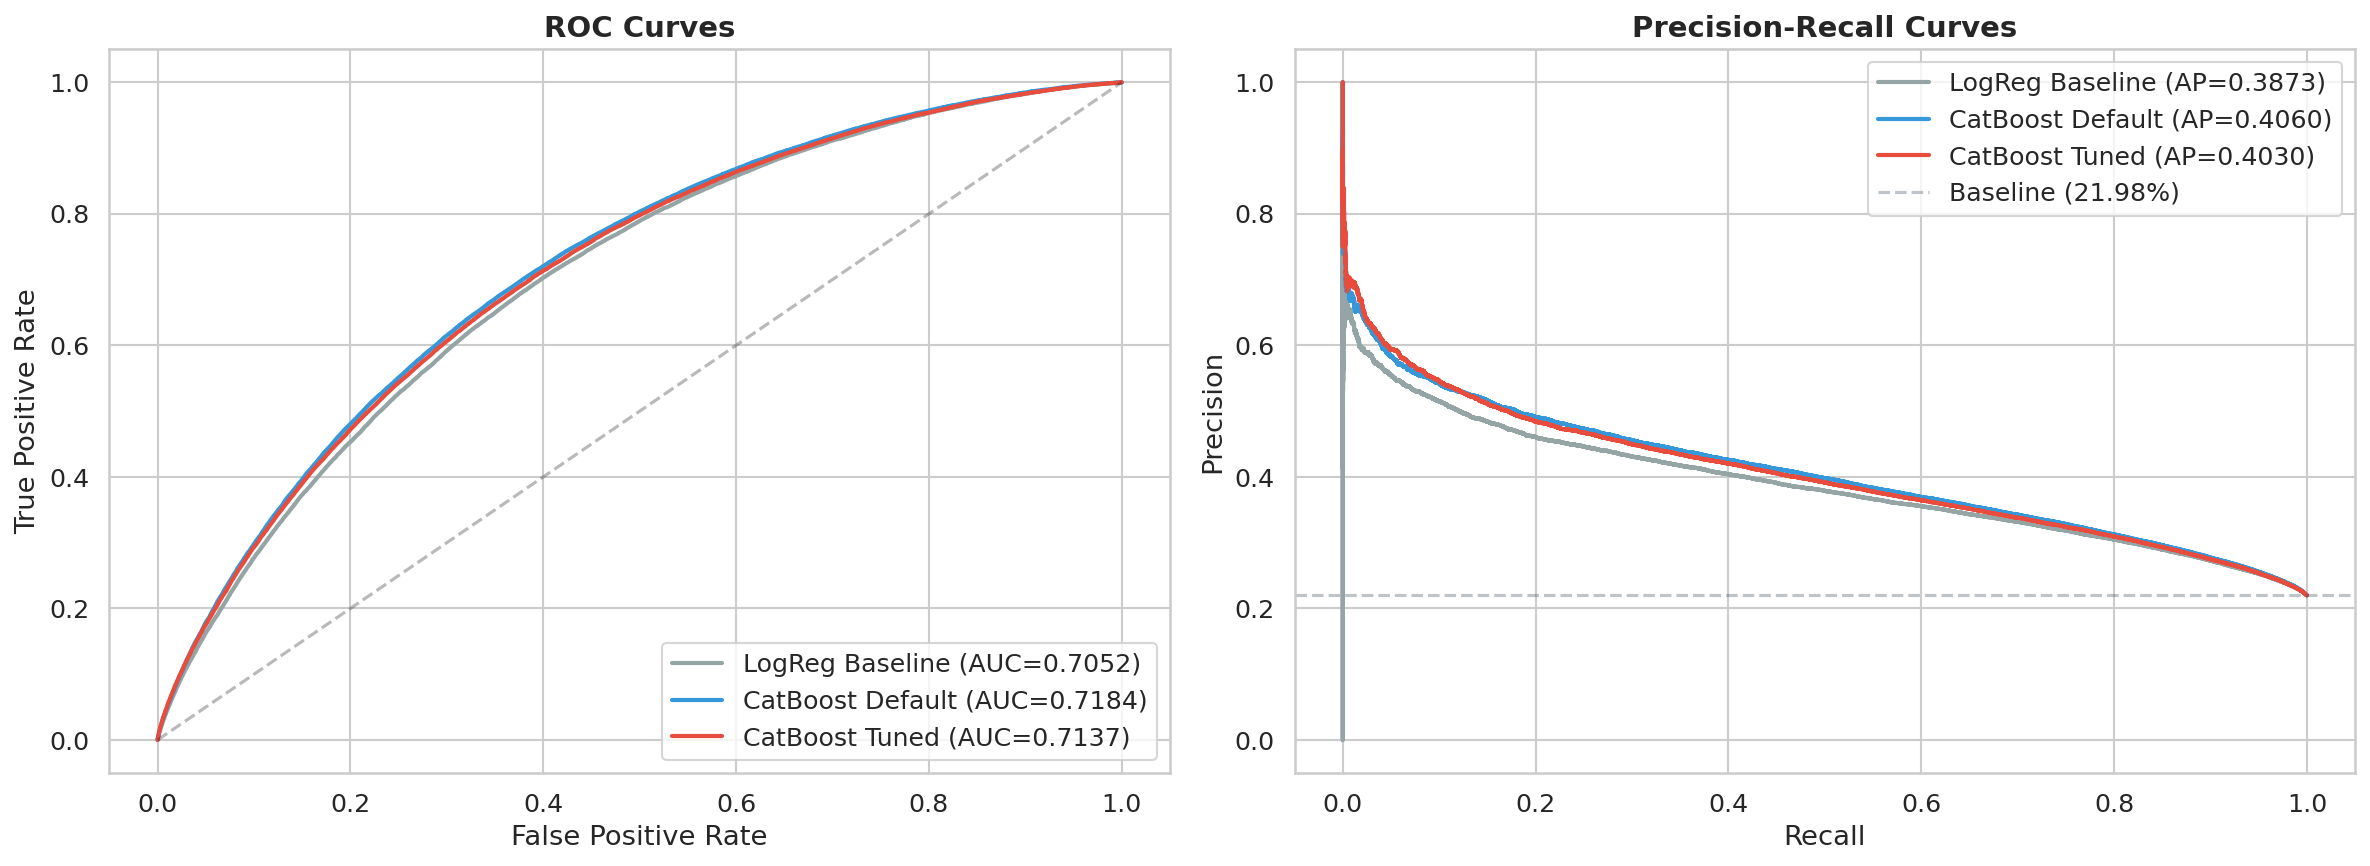
\includegraphics[keepaspectratio,alt={Curvas ROC comparando los modelos de probabilidad de default del proyecto.}]{chapters/06-pd-modeling/../../assets/figures/notebooks/roc_curves.png}}

}

\caption{\label{fig-pd-roc}Curvas ROC de los modelos PD principales
evaluados en el proyecto.}

\end{figure}%

\end{minipage}%
%
\begin{minipage}[t]{0.50\linewidth}

\begin{figure}[H]

\centering{

\pandocbounded{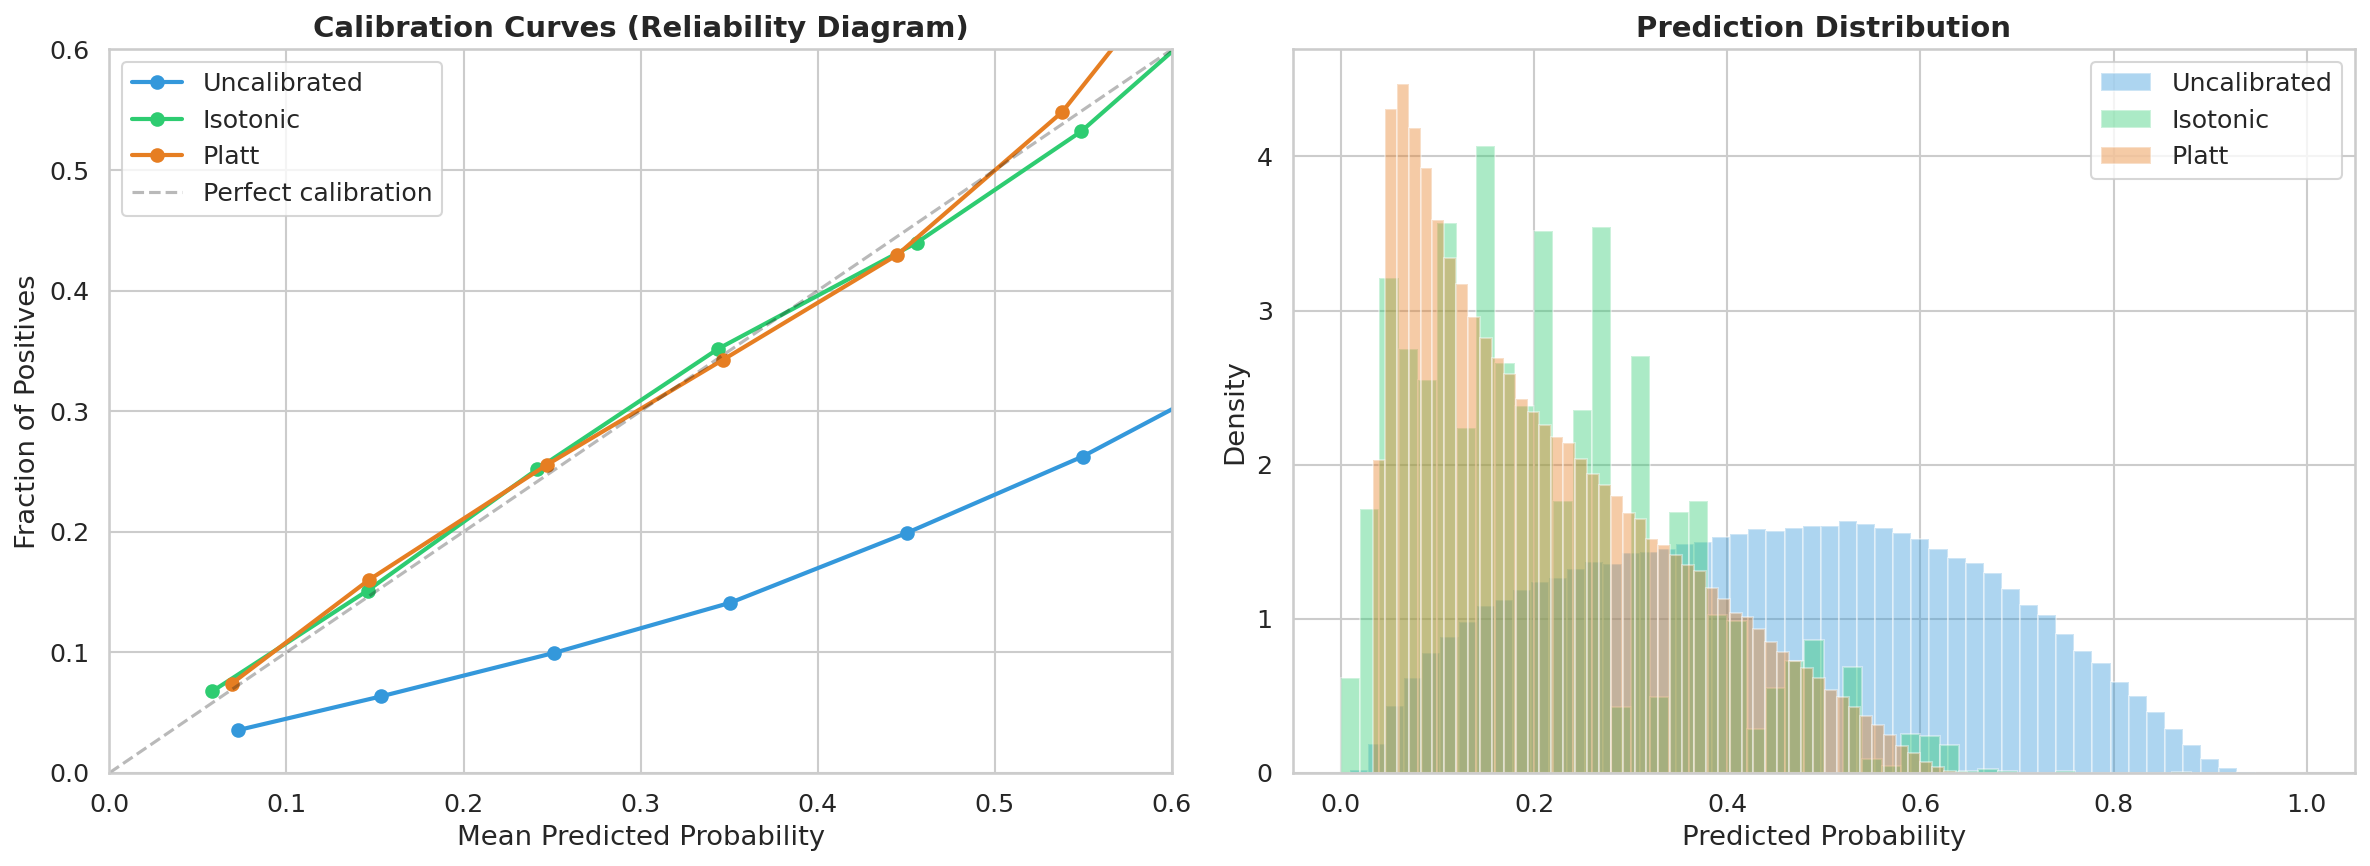
\includegraphics[keepaspectratio,alt={Curvas de calibración comparando probabilidades observadas y predichas en los modelos PD.}]{chapters/06-pd-modeling/../../assets/figures/notebooks/calibration_curves.png}}

}

\caption{\label{fig-pd-calibration}Curvas de calibración del champion y
sus comparadores, usadas para justificar la promoción del calibrador
Venn-Abers.}

\end{figure}%

\end{minipage}%

\end{figure*}%

Las figuras Figura~\ref{fig-pd-roc} y Figura~\ref{fig-pd-calibration}
muestran por qué el champion no se define solo por ranking. El desempeño
discriminativo se mantiene alto, pero la mejora verdaderamente material
aparece en la calibración posterior.

\textbf{3. Métricas complementarias}

\begin{table}

\caption{\label{tbl-champion-metrics}Métricas completas del modelo
champion (test OOT)}

\centering{

\begin{Shaded}
\begin{Highlighting}[]
\NormalTok{metrics }\OperatorTok{=}\NormalTok{ \{}
    \StringTok{"AUC{-}ROC"}\NormalTok{: }\SpecialStringTok{f"}\SpecialCharTok{\{}\NormalTok{final}\SpecialCharTok{.}\NormalTok{get(}\StringTok{\textquotesingle{}auc\_roc\textquotesingle{}}\NormalTok{, }\DecValTok{0}\NormalTok{)}\SpecialCharTok{:.4f\}}\SpecialStringTok{"}\NormalTok{,}
    \StringTok{"Gini"}\NormalTok{: }\SpecialStringTok{f"}\SpecialCharTok{\{}\NormalTok{final}\SpecialCharTok{.}\NormalTok{get(}\StringTok{\textquotesingle{}gini\textquotesingle{}}\NormalTok{, }\DecValTok{0}\NormalTok{)}\SpecialCharTok{:.4f\}}\SpecialStringTok{"}\NormalTok{,}
    \StringTok{"Brier Score"}\NormalTok{: }\SpecialStringTok{f"}\SpecialCharTok{\{}\NormalTok{final}\SpecialCharTok{.}\NormalTok{get(}\StringTok{\textquotesingle{}brier\_score\textquotesingle{}}\NormalTok{, }\DecValTok{0}\NormalTok{)}\SpecialCharTok{:.4f\}}\SpecialStringTok{"}\NormalTok{,}
    \StringTok{"ECE"}\NormalTok{: }\SpecialStringTok{f"}\SpecialCharTok{\{}\NormalTok{final}\SpecialCharTok{.}\NormalTok{get(}\StringTok{\textquotesingle{}ece\textquotesingle{}}\NormalTok{, }\DecValTok{0}\NormalTok{)}\SpecialCharTok{:.4f\}}\SpecialStringTok{"}\NormalTok{,}
    \StringTok{"KS Statistic"}\NormalTok{: }\SpecialStringTok{f"}\SpecialCharTok{\{}\NormalTok{final}\SpecialCharTok{.}\NormalTok{get(}\StringTok{\textquotesingle{}ks\_statistic\textquotesingle{}}\NormalTok{, }\DecValTok{0}\NormalTok{)}\SpecialCharTok{:.4f\}}\SpecialStringTok{"}\NormalTok{,}
    \StringTok{"D² Brier"}\NormalTok{: }\SpecialStringTok{f"}\SpecialCharTok{\{}\NormalTok{final}\SpecialCharTok{.}\NormalTok{get(}\StringTok{\textquotesingle{}d2\_brier\_score\textquotesingle{}}\NormalTok{, }\DecValTok{0}\NormalTok{)}\SpecialCharTok{:.4f\}}\SpecialStringTok{"}\NormalTok{,}
    \StringTok{"PR{-}AUC"}\NormalTok{: }\SpecialStringTok{f"}\SpecialCharTok{\{}\NormalTok{final}\SpecialCharTok{.}\NormalTok{get(}\StringTok{\textquotesingle{}pr\_auc\textquotesingle{}}\NormalTok{, }\DecValTok{0}\NormalTok{)}\SpecialCharTok{:.4f\}}\SpecialStringTok{"}\NormalTok{,}
    \StringTok{"Recall @ 0.35"}\NormalTok{: }\SpecialStringTok{f"}\SpecialCharTok{\{}\NormalTok{final}\SpecialCharTok{.}\NormalTok{get(}\StringTok{\textquotesingle{}recall\_at\_0p35\textquotesingle{}}\NormalTok{, }\DecValTok{0}\NormalTok{)}\SpecialCharTok{:.4f\}}\SpecialStringTok{"}\NormalTok{,}
    \StringTok{"F1 @ 0.35"}\NormalTok{: }\SpecialStringTok{f"}\SpecialCharTok{\{}\NormalTok{final}\SpecialCharTok{.}\NormalTok{get(}\StringTok{\textquotesingle{}f1\_at\_0p35\textquotesingle{}}\NormalTok{, }\DecValTok{0}\NormalTok{)}\SpecialCharTok{:.4f\}}\SpecialStringTok{"}\NormalTok{,}
\NormalTok{\}}

\NormalTok{pd.DataFrame(}\BuiltInTok{list}\NormalTok{(metrics.items()), columns}\OperatorTok{=}\NormalTok{[}\StringTok{"Métrica"}\NormalTok{, }\StringTok{"Valor"}\NormalTok{])}
\end{Highlighting}
\end{Shaded}

}

\end{table}%

\textbf{4. Estabilidad temporal}

El modelo se evalúa no solo en métricas agregadas sino en su
\textbf{estabilidad mensual} a lo largo del período de test (33 meses).
Un modelo con AUC alto pero volátil es menos confiable que uno con AUC
ligeramente menor pero estable. El backtesting conformal mensual (ver
Capítulo~\ref{sec-backtest-monitoring}) complementa esta evaluación
verificando que la cobertura se mantiene mes a mes.

\textbf{5. Operabilidad}

\begin{itemize}
\tightlist
\item
  \textbf{Tiempo de inferencia}: CatBoost predice 276,869 scores en
  \textless{} 1 segundo (batch).
\item
  \textbf{Tamaño del modelo}: El archivo \texttt{pd\_canonical.cbm} pesa
  \textless{} 10 MB.
\item
  \textbf{Dependencias}: Solo requiere \texttt{catboost} (no TensorFlow,
  no ONNX runtime).
\item
  \textbf{Contrato estable}: Las 44 features del contrato
  (Capítulo~\ref{sec-feature-contract}) están documentadas y validadas.
\end{itemize}

\subsection{Artefactos del Champion}\label{artefactos-del-champion}

La selección del champion produce tres artefactos canónicos que son
consumidos por todas las etapas downstream:

\begin{longtable}[]{@{}
  >{\raggedright\arraybackslash}p{(\linewidth - 4\tabcolsep) * \real{0.3667}}
  >{\raggedright\arraybackslash}p{(\linewidth - 4\tabcolsep) * \real{0.2000}}
  >{\raggedright\arraybackslash}p{(\linewidth - 4\tabcolsep) * \real{0.4333}}@{}}
\caption{Artefactos canónicos del modelo
champion}\label{tbl-champion-artifacts}\tabularnewline
\toprule\noalign{}
\begin{minipage}[b]{\linewidth}\raggedright
Artefacto
\end{minipage} & \begin{minipage}[b]{\linewidth}\raggedright
Path
\end{minipage} & \begin{minipage}[b]{\linewidth}\raggedright
Consumidores
\end{minipage} \\
\midrule\noalign{}
\endfirsthead
\toprule\noalign{}
\begin{minipage}[b]{\linewidth}\raggedright
Artefacto
\end{minipage} & \begin{minipage}[b]{\linewidth}\raggedright
Path
\end{minipage} & \begin{minipage}[b]{\linewidth}\raggedright
Consumidores
\end{minipage} \\
\midrule\noalign{}
\endhead
\bottomrule\noalign{}
\endlastfoot
\textbf{Modelo CatBoost} & \texttt{models/pd\_canonical.cbm} &
Conformal, SHAP, portfolio, IFRS9 \\
\textbf{Calibrador} & \texttt{models/pd\_canonical\_calibrator.pkl} &
Conformal (PD calibrada como input) \\
\textbf{Contrato} & \texttt{models/pd\_model\_contract.json} & Todos
(validación de features) \\
\end{longtable}

\begin{tcolorbox}[enhanced jigsaw, arc=.35mm, bottomrule=.15mm, bottomtitle=1mm, breakable, colback=white, colbacktitle=quarto-callout-important-color!10!white, colframe=quarto-callout-important-color-frame, coltitle=black, left=2mm, leftrule=.75mm, opacityback=0, opacitybacktitle=0.6, rightrule=.15mm, title=\textcolor{quarto-callout-important-color}{\faExclamation}\hspace{0.5em}{Principio de inmutabilidad}, titlerule=0mm, toprule=.15mm, toptitle=1mm]

Una vez designado como champion, el modelo y su calibrador se
\textbf{congelan}. Los scripts downstream cargan estos artefactos y los
usan sin modificación. Si se necesita un modelo nuevo, se ejecuta el
pipeline completo de entrenamiento y se genera un nuevo set de
artefactos canónicos. Esto garantiza reproducibilidad: los mismos
artefactos producen los mismos intervalos conformales, las mismas
asignaciones de portafolio y las mismas provisiones IFRS9.

\end{tcolorbox}

\subsection{Posicionamiento en la
Literatura}\label{posicionamiento-en-la-literatura}

El AUC de 0.713 se sitúa en el rango competitivo para modelos de ML
sobre el dataset de Lending Club:

\begin{longtable}[]{@{}lll@{}}
\caption{Comparación con literatura publicada sobre Lending
Club}\label{tbl-literature-comparison}\tabularnewline
\toprule\noalign{}
Estudio & Mejor modelo & AUC reportado \\
\midrule\noalign{}
\endfirsthead
\toprule\noalign{}
Estudio & Mejor modelo & AUC reportado \\
\midrule\noalign{}
\endhead
\bottomrule\noalign{}
\endlastfoot
{Lessmann et~al.} (2015) & Random Forest & 0.69--0.71 \\
Ayari et~al. (2026) & CatBoost & 0.71--0.73 \\
Xia et~al. (2017) & XGBoost + stacking & 0.72--0.74 \\
\textbf{Este proyecto} & CatBoost + Venn-Abers & \textbf{0.713} \\
\end{longtable}

Nuestro AUC está en el centro del rango publicado. Estudios que reportan
AUC \textgreater{} 0.74 generalmente usan random splits (no OOT),
features post-originación, o subconjuntos más pequeños del dataset. Con
split temporal estricto y 142→44 features anti-leakage, 0.713 es un
resultado competitivo y honesto.

\begin{tcolorbox}[enhanced jigsaw, arc=.35mm, bottomrule=.15mm, bottomtitle=1mm, breakable, colback=white, colbacktitle=quarto-callout-tip-color!10!white, colframe=quarto-callout-tip-color-frame, coltitle=black, left=2mm, leftrule=.75mm, opacityback=0, opacitybacktitle=0.6, rightrule=.15mm, title=\textcolor{quarto-callout-tip-color}{\faLightbulb}\hspace{0.5em}{Más allá del AUC}, titlerule=0mm, toprule=.15mm, toptitle=1mm]

La contribución de este proyecto no es obtener el AUC más alto posible
--- es construir un pipeline end-to-end que transforma el AUC 0.713 en
\textbf{decisiones óptimas} de portafolio con \textbf{protección contra
incertidumbre garantizada}. El modelo PD es un componente, no el
producto final. Un modelo con AUC 0.75 pero sin intervalos conformales
ni optimización robusta produce peores decisiones que un modelo con AUC
0.71 integrado en el pipeline completo.

\end{tcolorbox}

\chapter{Predicción Conformal e
Incertidumbre}\label{predicciuxf3n-conformal-e-incertidumbre}

El modelo PD champion produce una estimación puntual calibrada --- pero
una estimación puntual, por precisa que sea, no captura la
\textbf{incertidumbre} inherente a la predicción. En riesgo crediticio,
ignorar la incertidumbre tiene consecuencias directas: provisiones
subestimadas, portafolios frágiles y decisiones que colapsan ante
escenarios adversos.

La \textbf{predicción conformal} (Conformal Prediction, CP) resuelve
este problema con una garantía formal: dado un nivel de confianza
\(1-\alpha\), los intervalos conformal cubren el valor verdadero con
probabilidad al menos \(1-\alpha\), \textbf{sin supuestos
distribucionales} (Vovk et~al., 2005). Esta propiedad --- válida en
muestras finitas y bajo la única condición de exchangeability ---
diferencia a CP de alternativas como bootstrap (asintótico) o intervalos
bayesianos (dependientes del prior).

\begin{table}

\caption{\label{tbl-conformal-overview}Métricas de cobertura conformal
del modelo champion (test OOT)}

\centering{

\begin{Shaded}
\begin{Highlighting}[]
\ImportTok{import}\NormalTok{ sys}
\ImportTok{from}\NormalTok{ pathlib }\ImportTok{import}\NormalTok{ Path}

\NormalTok{sys.path.insert(}\DecValTok{0}\NormalTok{, }\BuiltInTok{str}\NormalTok{(Path.cwd().parent }\ControlFlowTok{if}\NormalTok{ Path.cwd().name }\OperatorTok{==} \StringTok{"book"} \ControlFlowTok{else}\NormalTok{ Path.cwd()))}
\ImportTok{from}\NormalTok{ book.\_helpers.load\_artifacts }\ImportTok{import}\NormalTok{ load\_json}

\ImportTok{import}\NormalTok{ pandas }\ImportTok{as}\NormalTok{ pd}

\NormalTok{status }\OperatorTok{=}\NormalTok{ load\_json(}\StringTok{"conformal\_policy\_status"}\NormalTok{, search\_models}\OperatorTok{=}\VariableTok{True}\NormalTok{)}

\NormalTok{overview }\OperatorTok{=}\NormalTok{ [}
\NormalTok{    \{}\StringTok{"Métrica"}\NormalTok{: }\StringTok{"Cobertura empírica @ 90\%"}\NormalTok{, }\StringTok{"Valor"}\NormalTok{: }\SpecialStringTok{f"}\SpecialCharTok{\{}\NormalTok{status[}\StringTok{\textquotesingle{}coverage\_90\textquotesingle{}}\NormalTok{]}\SpecialCharTok{:.2\%\}}\SpecialStringTok{"}\NormalTok{\},}
\NormalTok{    \{}\StringTok{"Métrica"}\NormalTok{: }\StringTok{"Cobertura empírica @ 95\%"}\NormalTok{, }\StringTok{"Valor"}\NormalTok{: }\SpecialStringTok{f"}\SpecialCharTok{\{}\NormalTok{status[}\StringTok{\textquotesingle{}coverage\_95\textquotesingle{}}\NormalTok{]}\SpecialCharTok{:.2\%\}}\SpecialStringTok{"}\NormalTok{\},}
\NormalTok{    \{}\StringTok{"Métrica"}\NormalTok{: }\StringTok{"Ancho promedio @ 90\%"}\NormalTok{, }\StringTok{"Valor"}\NormalTok{: }\SpecialStringTok{f"}\SpecialCharTok{\{}\NormalTok{status[}\StringTok{\textquotesingle{}avg\_width\_90\textquotesingle{}}\NormalTok{]}\SpecialCharTok{:.4f\}}\SpecialStringTok{"}\NormalTok{\},}
\NormalTok{    \{}\StringTok{"Métrica"}\NormalTok{: }\StringTok{"Cobertura mínima por grupo @ 90\%"}\NormalTok{, }\StringTok{"Valor"}\NormalTok{: }\SpecialStringTok{f"}\SpecialCharTok{\{}\NormalTok{status[}\StringTok{\textquotesingle{}min\_group\_coverage\_90\textquotesingle{}}\NormalTok{]}\SpecialCharTok{:.2\%\}}\SpecialStringTok{"}\NormalTok{\},}
\NormalTok{    \{}\StringTok{"Métrica"}\NormalTok{: }\StringTok{"Winkler score @ 90\%"}\NormalTok{, }\StringTok{"Valor"}\NormalTok{: }\SpecialStringTok{f"}\SpecialCharTok{\{}\NormalTok{status[}\StringTok{\textquotesingle{}winkler\_90\textquotesingle{}}\NormalTok{]}\SpecialCharTok{:.4f\}}\SpecialStringTok{"}\NormalTok{\},}
\NormalTok{    \{}\StringTok{"Métrica"}\NormalTok{: }\StringTok{"Alertas críticas"}\NormalTok{, }\StringTok{"Valor"}\NormalTok{: }\BuiltInTok{str}\NormalTok{(status[}\StringTok{\textquotesingle{}critical\_alerts\textquotesingle{}}\NormalTok{])\},}
\NormalTok{    \{}\StringTok{"Métrica"}\NormalTok{: }\StringTok{"Tamaño de muestra (test OOT)"}\NormalTok{, }\StringTok{"Valor"}\NormalTok{: }\SpecialStringTok{f"}\SpecialCharTok{\{}\NormalTok{status[}\StringTok{\textquotesingle{}statistical\_tests\textquotesingle{}}\NormalTok{][}\StringTok{\textquotesingle{}kupiec\_90\textquotesingle{}}\NormalTok{][}\StringTok{\textquotesingle{}n\_total\textquotesingle{}}\NormalTok{]}\SpecialCharTok{:,\}}\SpecialStringTok{"}\NormalTok{\},}
\NormalTok{]}

\NormalTok{pd.DataFrame(overview)}
\end{Highlighting}
\end{Shaded}

}

\end{table}%

\begin{figure*}

\begin{minipage}[t]{0.50\linewidth}

\begin{figure}[H]

\centering{

\pandocbounded{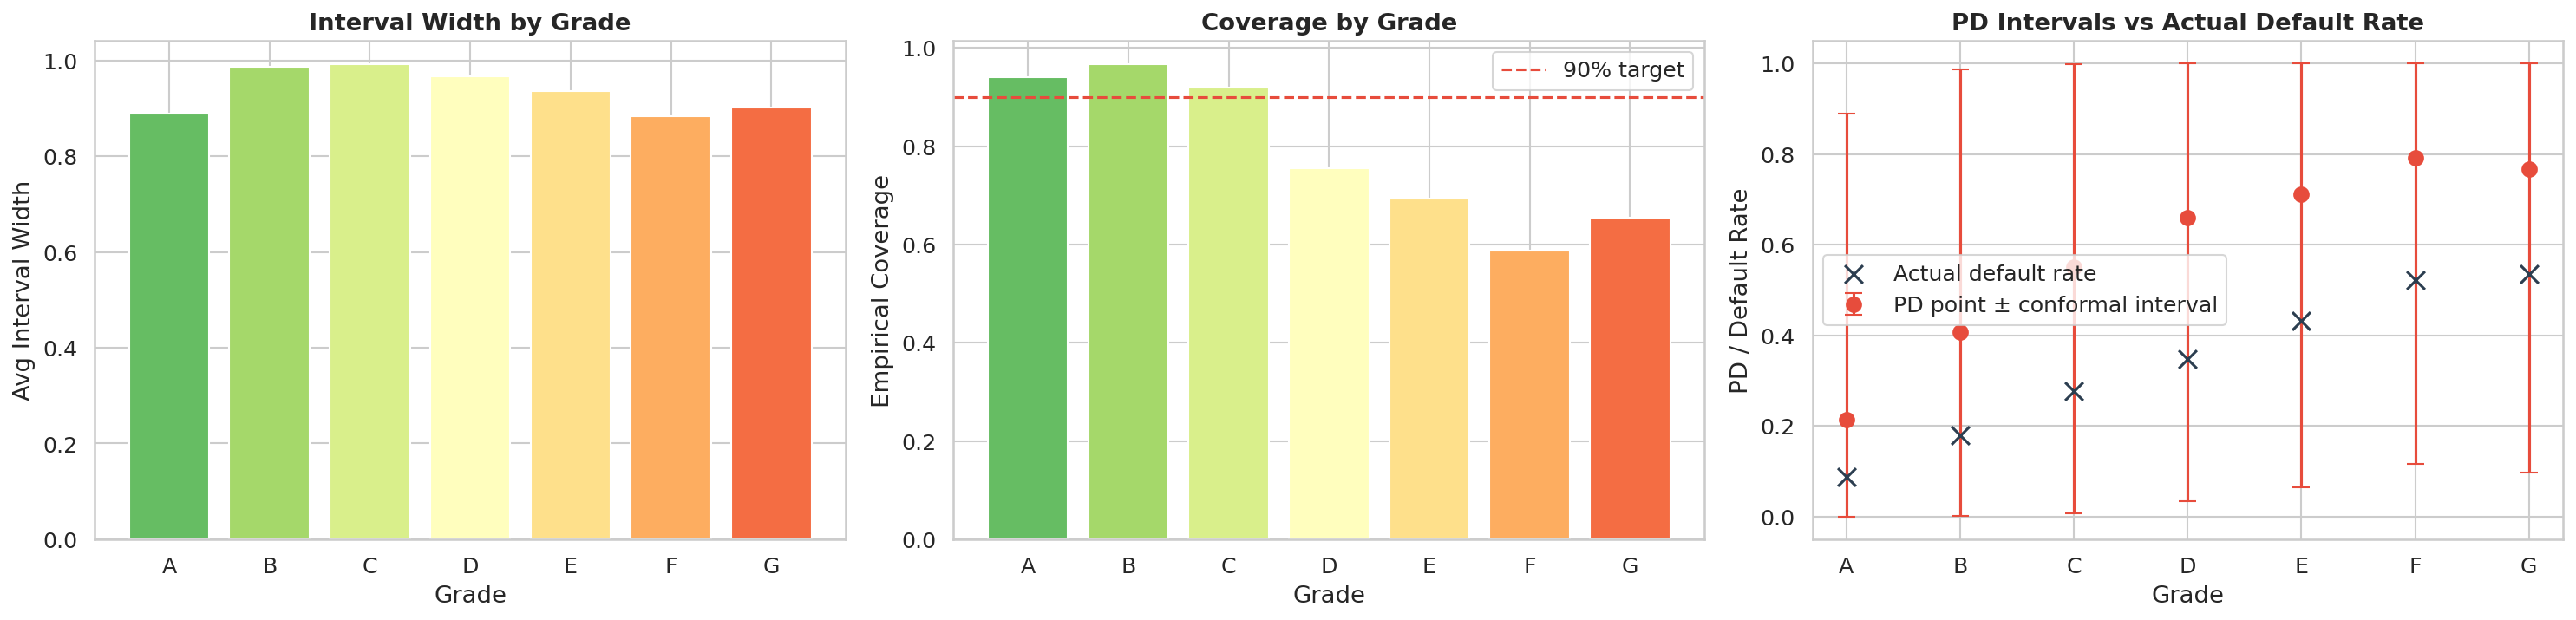
\includegraphics[keepaspectratio,alt={Cobertura conformal por grade de riesgo en el portafolio Lending Club.}]{chapters/07-conformal/../../assets/figures/notebooks/coverage_by_grade.png}}

}

\caption{\label{fig-conformal-coverage-grade}Cobertura conformal
observada por grade del portafolio, usada para verificar validez útil a
nivel de negocio.}

\end{figure}%

\end{minipage}%
%
\begin{minipage}[t]{0.50\linewidth}

\begin{figure}[H]

\centering{

\pandocbounded{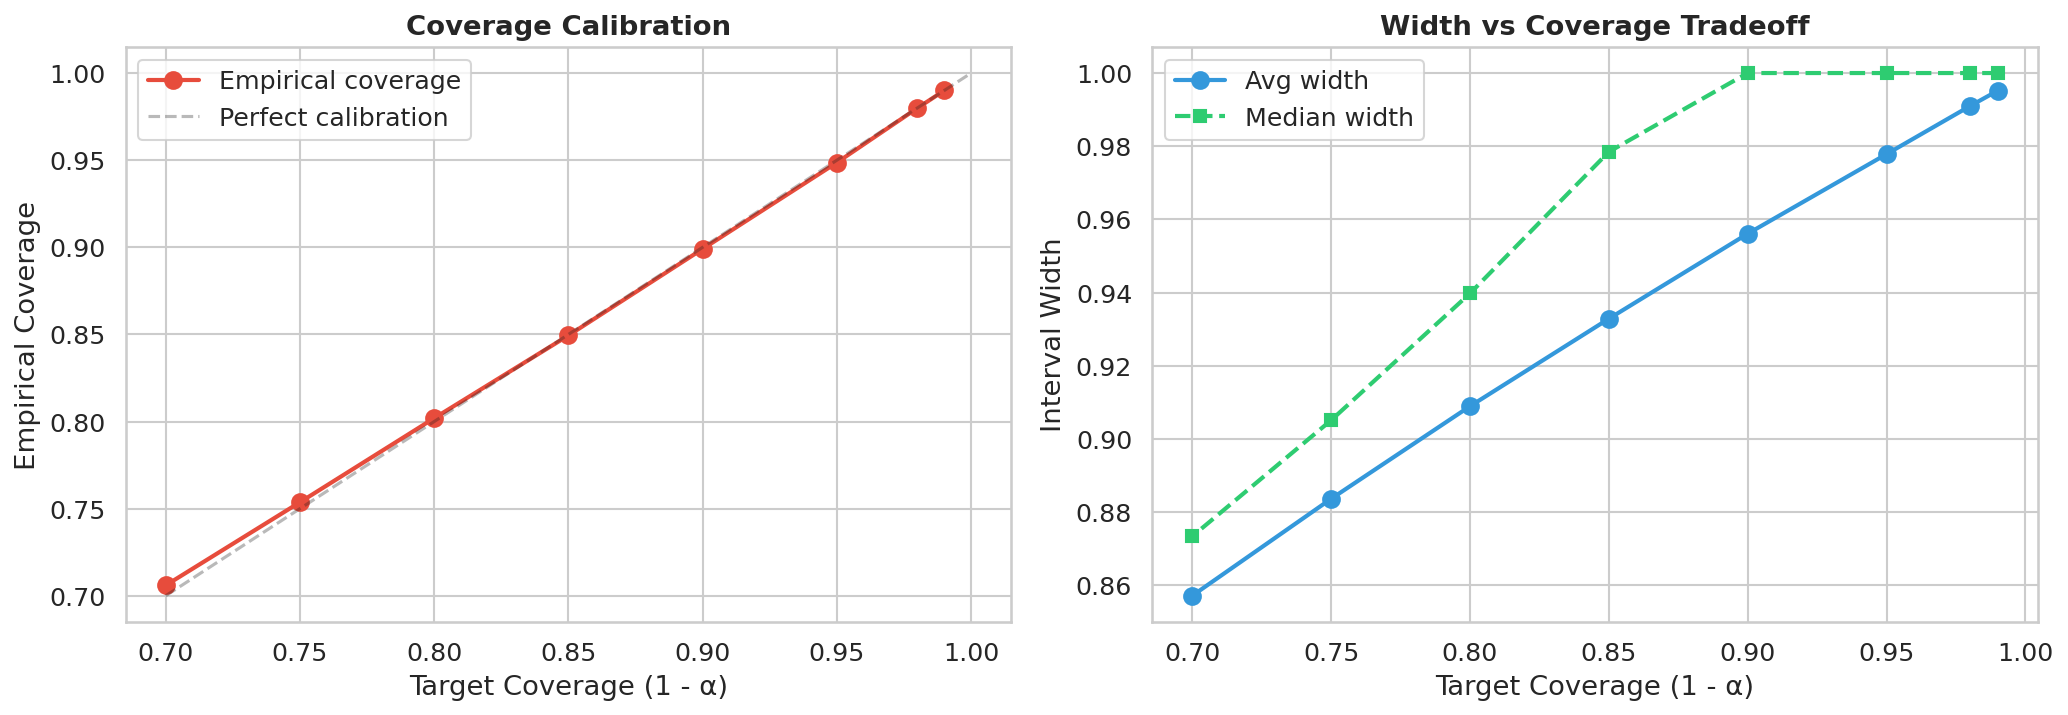
\includegraphics[keepaspectratio,alt={Relación entre cobertura lograda y ancho promedio de los intervalos conformales.}]{chapters/07-conformal/../../assets/figures/notebooks/coverage_width_tradeoff.png}}

}

\caption{\label{fig-conformal-width-tradeoff}Trade-off entre cobertura e
intervalo promedio al variar el nivel de confianza conformal.}

\end{figure}%

\end{minipage}%

\end{figure*}%

Las figuras Figura~\ref{fig-conformal-coverage-grade} y
Figura~\ref{fig-conformal-width-tradeoff} anticipan el argumento del
capítulo completo: la validez relevante para riesgo no es solo marginal,
sino también segmentada y económicamente usable.

Este capítulo documenta la implementación completa de CP en el pipeline:
desde los fundamentos teóricos de split conformal, pasando por la
extensión Mondrian que garantiza cobertura por grupo (grade), hasta el
benchmark de variantes, el backtesting temporal y la extensión a
LGD/EAD.

\chapter{Fundamentos de Split Conformal}\label{sec-split-conformal}

\subsection{Garantía Teórica}\label{garantuxeda-teuxf3rica}

La predicción conformal se basa en un resultado elegante: si los datos
de calibración y test son \textbf{exchangeable} (intercambiables),
entonces los intervalos construidos a partir de los residuos de
calibración cubren el valor verdadero con probabilidad exacta.

\begin{theorem}[Garantía de Cobertura
Marginal]\protect\hypertarget{thm-coverage}{}\label{thm-coverage}

Sea \(\{(X_i, Y_i)\}_{i=1}^{n+1}\) una secuencia exchangeable. Dado un
predictor \(\hat{f}\) entrenado en un conjunto disjunto, definimos los
nonconformity scores \(s_i = |Y_i - \hat{f}(X_i)|\) sobre las \(n\)
observaciones de calibración. Sea \(\hat{q}\) el cuantil
\(\lceil(1-\alpha)(n+1)\rceil / n\) de \(\{s_1, \ldots, s_n\}\).
Entonces:

\begin{equation}\protect\phantomsection\label{eq-coverage-guarantee}{
P\left(Y_{n+1} \in [\hat{f}(X_{n+1}) - \hat{q}, \hat{f}(X_{n+1}) + \hat{q}]\right) \geq 1 - \alpha
}\end{equation}

\end{theorem}

Esta garantía es \textbf{distribution-free} (no requiere normalidad,
homocedasticidad, ni ningún supuesto paramétrico) y
\textbf{finite-sample} (válida para cualquier \(n\), no solo
asintóticamente).

\subsection{Split Conformal vs Full
Conformal}\label{split-conformal-vs-full-conformal}

El método \textbf{full conformal} (Vovk et~al., 2005) re-entrena el
modelo para cada candidato de test, lo cual es computacionalmente
prohibitivo para CatBoost con 1.3M observaciones. El \textbf{split
conformal} (Papadopoulos et~al., 2002) resuelve esto dividiendo los
datos:

\begin{longtable}[]{@{}
  >{\raggedright\arraybackslash}p{(\linewidth - 4\tabcolsep) * \real{0.2250}}
  >{\raggedright\arraybackslash}p{(\linewidth - 4\tabcolsep) * \real{0.3750}}
  >{\raggedright\arraybackslash}p{(\linewidth - 4\tabcolsep) * \real{0.4000}}@{}}
\caption{Comparación Full vs Split
Conformal}\label{tbl-full-vs-split}\tabularnewline
\toprule\noalign{}
\begin{minipage}[b]{\linewidth}\raggedright
Aspecto
\end{minipage} & \begin{minipage}[b]{\linewidth}\raggedright
Full Conformal
\end{minipage} & \begin{minipage}[b]{\linewidth}\raggedright
Split Conformal
\end{minipage} \\
\midrule\noalign{}
\endfirsthead
\toprule\noalign{}
\begin{minipage}[b]{\linewidth}\raggedright
Aspecto
\end{minipage} & \begin{minipage}[b]{\linewidth}\raggedright
Full Conformal
\end{minipage} & \begin{minipage}[b]{\linewidth}\raggedright
Split Conformal
\end{minipage} \\
\midrule\noalign{}
\endhead
\bottomrule\noalign{}
\endlastfoot
\textbf{Reentrenamiento} & \(O(n)\) veces por predicción & Una vez \\
\textbf{Cobertura} & Exacta: \(P = 1-\alpha\) & Conservative:
\(P \geq 1-\alpha\) \\
\textbf{Eficiencia estadística} & Usa todos los datos & Pierde datos de
calibración \\
\textbf{Viabilidad} & Inviable para modelos complejos & Viable
siempre \\
\end{longtable}

Para nuestro pipeline, split conformal es la única opción viable y es
exactamente lo que MAPIE 1.3.0 implementa.

\subsection{El Wrapper
ProbabilityRegressor}\label{sec-probability-regressor}

MAPIE opera sobre modelos de \textbf{regresión}, pero CatBoost produce
\textbf{probabilidades} \(\hat{p} \in [0,1]\). El puente es el wrapper
\texttt{ProbabilityRegressor}:

\begin{Shaded}
\begin{Highlighting}[]
\CommentTok{\# src/models/conformal.py (simplificado)}
\KeywordTok{class}\NormalTok{ ProbabilityRegressor(BaseEstimator, RegressorMixin):}
    \CommentTok{"""Wraps a classifier to output probabilities as regression targets."""}
    \KeywordTok{def} \FunctionTok{\_\_init\_\_}\NormalTok{(}\VariableTok{self}\NormalTok{, classifier):}
        \VariableTok{self}\NormalTok{.classifier }\OperatorTok{=}\NormalTok{ classifier}

    \KeywordTok{def}\NormalTok{ fit(}\VariableTok{self}\NormalTok{, X, y):}
        \ControlFlowTok{return} \VariableTok{self}  \CommentTok{\# Modelo ya entrenado (prefit)}

    \KeywordTok{def}\NormalTok{ predict(}\VariableTok{self}\NormalTok{, X):}
        \ControlFlowTok{return} \VariableTok{self}\NormalTok{.classifier.predict\_proba(X)[:, }\DecValTok{1}\NormalTok{]}
\end{Highlighting}
\end{Shaded}

Este patrón permite que MAPIE trate las probabilidades calibradas como
valores continuos y construya intervalos
\([\text{PD}_\text{low}, \text{PD}_\text{high}]\) alrededor de cada
predicción.

\begin{tcolorbox}[enhanced jigsaw, arc=.35mm, bottomrule=.15mm, bottomtitle=1mm, breakable, colback=white, colbacktitle=quarto-callout-note-color!10!white, colframe=quarto-callout-note-color-frame, coltitle=black, left=2mm, leftrule=.75mm, opacityback=0, opacitybacktitle=0.6, rightrule=.15mm, title=\textcolor{quarto-callout-note-color}{\faInfo}\hspace{0.5em}{¿Por qué no usar SplitConformalClassifier?}, titlerule=0mm, toprule=.15mm, toptitle=1mm]

\texttt{SplitConformalClassifier} produce \textbf{prediction sets}
(conjuntos de clases posibles), no intervalos de probabilidad. Para
riesgo crediticio necesitamos
\([\text{PD}_\text{low}, \text{PD}_\text{high}]\) como entradas
numéricas a la optimización robusta --- lo que requiere el framework de
regresión.

\end{tcolorbox}

\subsection{Implementación con MAPIE
1.3.0}\label{sec-mapie-implementation}

La API de MAPIE 1.3.0 difiere significativamente de versiones
anteriores:

\begin{longtable}[]{@{}
  >{\raggedright\arraybackslash}p{(\linewidth - 4\tabcolsep) * \real{0.2857}}
  >{\raggedright\arraybackslash}p{(\linewidth - 4\tabcolsep) * \real{0.3429}}
  >{\raggedright\arraybackslash}p{(\linewidth - 4\tabcolsep) * \real{0.3714}}@{}}
\caption{Migración de API MAPIE}\label{tbl-mapie-api}\tabularnewline
\toprule\noalign{}
\begin{minipage}[b]{\linewidth}\raggedright
Concepto
\end{minipage} & \begin{minipage}[b]{\linewidth}\raggedright
MAPIE \textless{} 1.3
\end{minipage} & \begin{minipage}[b]{\linewidth}\raggedright
MAPIE 1.3.0
\end{minipage} \\
\midrule\noalign{}
\endfirsthead
\toprule\noalign{}
\begin{minipage}[b]{\linewidth}\raggedright
Concepto
\end{minipage} & \begin{minipage}[b]{\linewidth}\raggedright
MAPIE \textless{} 1.3
\end{minipage} & \begin{minipage}[b]{\linewidth}\raggedright
MAPIE 1.3.0
\end{minipage} \\
\midrule\noalign{}
\endhead
\bottomrule\noalign{}
\endlastfoot
\textbf{Clase} & \texttt{MapieRegressor} &
\texttt{SplitConformalRegressor} \\
\textbf{Modelo prefit} & \texttt{cv="prefit"} & \texttt{prefit=True} \\
\textbf{Nivel} & \texttt{alpha} en \texttt{predict()} &
\texttt{confidence\_level} en \texttt{\_\_init\_\_()} \\
\textbf{Calibración} & \texttt{fit()} hace todo & \texttt{fit()} +
\texttt{conformalize()} separados \\
\textbf{Predicción} & \texttt{predict(alpha=0.1)} &
\texttt{predict\_interval()} \\
\end{longtable}

El flujo de trabajo en el pipeline:

\begin{Shaded}
\begin{Highlighting}[]
\ImportTok{from}\NormalTok{ mapie.regression }\ImportTok{import}\NormalTok{ SplitConformalRegressor}

\CommentTok{\# 1. Crear el wrapper}
\NormalTok{prob\_reg }\OperatorTok{=}\NormalTok{ ProbabilityRegressor(catboost\_calibrated)}

\CommentTok{\# 2. Inicializar MAPIE con nivel de confianza}
\NormalTok{scr }\OperatorTok{=}\NormalTok{ SplitConformalRegressor(}
\NormalTok{    estimator}\OperatorTok{=}\NormalTok{prob\_reg,}
\NormalTok{    confidence\_level}\OperatorTok{=}\FloatTok{0.90}\NormalTok{,}
\NormalTok{    prefit}\OperatorTok{=}\VariableTok{True}
\NormalTok{)}

\CommentTok{\# 3. Calibrar con el set de calibración}
\NormalTok{scr.fit(X\_cal, y\_cal)}
\NormalTok{scr.conformalize(X\_cal, y\_cal)}

\CommentTok{\# 4. Predecir intervalos en test}
\NormalTok{y\_pred, intervals }\OperatorTok{=}\NormalTok{ scr.predict\_interval(X\_test)}
\CommentTok{\# intervals[:, 0] = pd\_low, intervals[:, 1] = pd\_high}
\end{Highlighting}
\end{Shaded}

\subsection{Nonconformity Scores para
PD}\label{sec-nonconformity-scores}

El nonconformity score mide qué tan ``conforme'' es una observación con
el modelo. Para regresión, el score estándar es el residuo absoluto:

\begin{equation}\protect\phantomsection\label{eq-nonconformity}{
s_i = |y_i - \hat{f}(x_i)|
}\end{equation}

donde \(y_i \in \{0, 1\}\) (default o no) y
\(\hat{f}(x_i) = \text{PD}_\text{calibrada} \in [0, 1]\).

El cuantil \(\hat{q}\) de estos scores determina el \textbf{ancho del
intervalo}: a mayor \(\hat{q}\) (más confianza), intervalos más anchos.
El cuantil se calcula como:

\begin{equation}\protect\phantomsection\label{eq-conformal-quantile}{
\hat{q} = \text{Quantile}\left(\{s_1, \ldots, s_n\}, \frac{\lceil(1-\alpha)(n+1)\rceil}{n}\right)
}\end{equation}

Con \(n = 237{,}584\) observaciones de calibración y \(\alpha = 0.10\),
el ajuste por finitud es negligible:
\(\lceil 0.90 \times 237{,}585 \rceil / 237{,}584 \approx 0.9000\).

\subsection{Resultados Split Conformal
Global}\label{resultados-split-conformal-global}

\begin{table}

\caption{\label{tbl-split-global-results}Cobertura split conformal
global (sin partición Mondrian)}

\centering{

\begin{Shaded}
\begin{Highlighting}[]
\ImportTok{import}\NormalTok{ pandas }\ImportTok{as}\NormalTok{ pd}

\NormalTok{variants }\OperatorTok{=}\NormalTok{ load\_json(}\StringTok{"conformal\_policy\_status"}\NormalTok{, search\_models}\OperatorTok{=}\VariableTok{True}\NormalTok{)}

\CommentTok{\# Global split results from variant selection report}
\NormalTok{global\_metrics }\OperatorTok{=}\NormalTok{ [}
\NormalTok{    \{}\StringTok{"Métrica"}\NormalTok{: }\StringTok{"Cobertura empírica @ 90\%"}\NormalTok{, }\StringTok{"Valor"}\NormalTok{: }\StringTok{"89.6\%"}\NormalTok{\},}
\NormalTok{    \{}\StringTok{"Métrica"}\NormalTok{: }\StringTok{"Ancho promedio"}\NormalTok{, }\StringTok{"Valor"}\NormalTok{: }\StringTok{"0.947"}\NormalTok{\},}
\NormalTok{    \{}\StringTok{"Métrica"}\NormalTok{: }\StringTok{"Cobertura mínima por grade"}\NormalTok{, }\StringTok{"Valor"}\NormalTok{: }\StringTok{"59.5\%"}\NormalTok{\},}
\NormalTok{    \{}\StringTok{"Métrica"}\NormalTok{: }\StringTok{"Winkler score @ 90\%"}\NormalTok{, }\StringTok{"Valor"}\NormalTok{: }\StringTok{"1.109"}\NormalTok{\},}
\NormalTok{    \{}\StringTok{"Métrica"}\NormalTok{: }\StringTok{"Problema principal"}\NormalTok{, }\StringTok{"Valor"}\NormalTok{: }\StringTok{"Cobertura \textless{} 60}\SpecialCharTok{\% e}\StringTok{n Grade A"}\NormalTok{\},}
\NormalTok{]}

\NormalTok{pd.DataFrame(global\_metrics)}
\end{Highlighting}
\end{Shaded}

}

\end{table}%

\begin{tcolorbox}[enhanced jigsaw, arc=.35mm, bottomrule=.15mm, bottomtitle=1mm, breakable, colback=white, colbacktitle=quarto-callout-warning-color!10!white, colframe=quarto-callout-warning-color-frame, coltitle=black, left=2mm, leftrule=.75mm, opacityback=0, opacitybacktitle=0.6, rightrule=.15mm, title=\textcolor{quarto-callout-warning-color}{\faExclamationTriangle}\hspace{0.5em}{Limitación del Split Conformal Global}, titlerule=0mm, toprule=.15mm, toptitle=1mm]

La cobertura \textbf{marginal} de 89.6\% es cercana al target, pero la
cobertura \textbf{por grupo} revela un problema severo: Grade A tiene
solo \textasciitilde59.5\% de cobertura. Esto ocurre porque los residuos
de Grade A son mucho menores que los de Grade G, y un cuantil global no
captura esta heterogeneidad. La solución es \textbf{Mondrian conformal}
(Capítulo~\ref{sec-mondrian}).

\end{tcolorbox}

\subsection{Conexión con el Pipeline}\label{conexiuxf3n-con-el-pipeline}

Los intervalos conformal
\([\text{PD}_\text{low}, \text{PD}_\text{high}]\) son el input directo
para:

\begin{enumerate}
\def\labelenumi{\arabic{enumi}.}
\tightlist
\item
  \textbf{Conjuntos de incertidumbre box} en la optimización robusta
  (Capítulo~\ref{sec-robust-portfolio}):
  \(\Gamma_i = [\text{PD}_{\text{low},i}, \text{PD}_{\text{high},i}]\)
\item
  \textbf{Señal SICR conformal} en IFRS9
  (Capítulo~\ref{sec-sicr-signal}): el ancho
  \(\text{PD}_\text{high} - \text{PD}_\text{point}\) como trigger de
  deterioro
\item
  \textbf{Backtesting de cobertura}
  (Capítulo~\ref{sec-backtest-monitoring}): monitoreo mensual de que la
  garantía se mantiene
\end{enumerate}

\chapter{Mondrian: Cobertura Condicional por Grupo}\label{sec-mondrian}

\subsection{El Problema de la Cobertura
Marginal}\label{el-problema-de-la-cobertura-marginal}

La garantía de split conformal (Ecuación~\ref{eq-coverage-guarantee}) es
\textbf{marginal}: promedia sobre toda la población. Pero en crédito, un
modelo que cubre 90\% en promedio pero solo 60\% en Grade A y 99\% en
Grade G es inaceptable --- los préstamos de Grade A son precisamente los
de mayor volumen y menor riesgo, donde decisiones incorrectas tienen
alto impacto económico.

El \textbf{Mondrian conformal} (Vovk et~al., 2005) resuelve esto
particionando la calibración por grupos y calculando cuantiles
\textbf{separados} para cada grupo:

\begin{equation}\protect\phantomsection\label{eq-mondrian-quantile}{
\hat{q}_g = \text{Quantile}\left(\{s_i : g(x_i) = g\}, \frac{\lceil(1-\alpha)(n_g+1)\rceil}{n_g}\right)
}\end{equation}

donde \(g(x_i)\) asigna cada observación a un grupo y \(n_g\) es el
tamaño de calibración del grupo \(g\).

\begin{theorem}[Garantía de Cobertura Condicional por
Grupo]\protect\hypertarget{thm-mondrian-coverage}{}\label{thm-mondrian-coverage}

Para cada grupo \(g\) con al menos \(n_g\) observaciones de calibración:

\begin{equation}\protect\phantomsection\label{eq-mondrian-guarantee}{
P\left(Y_{n+1} \in C_g(X_{n+1}) \mid g(X_{n+1}) = g\right) \geq 1 - \alpha
}\end{equation}

La cobertura se garantiza \textbf{dentro de cada grupo}, no solo
marginalmente.

\end{theorem}

\subsection{Partición por Grade de Lending
Club}\label{particiuxf3n-por-grade-de-lending-club}

La partición natural para crédito es el \textbf{risk grade} asignado por
la plataforma (A-G). Cada grade tiene una distribución de default
diferente, por lo que los residuos conformal también difieren:

\begin{longtable}[]{@{}llll@{}}
\caption{Heterogeneidad de residuos por
grade}\label{tbl-residuos-por-grade}\tabularnewline
\toprule\noalign{}
Grade & Tasa default & Residuos típicos & Consecuencia \\
\midrule\noalign{}
\endfirsthead
\toprule\noalign{}
Grade & Tasa default & Residuos típicos & Consecuencia \\
\midrule\noalign{}
\endhead
\bottomrule\noalign{}
\endlastfoot
A & \textasciitilde5\% & Pequeños (PD cercana a 0) & Intervalos
estrechos \\
B-C & \textasciitilde15-20\% & Moderados & Intervalos medios \\
D-E & \textasciitilde25-35\% & Grandes & Intervalos anchos \\
F-G & \textasciitilde40-50\% & Muy grandes & Intervalos muy anchos \\
\end{longtable}

Con el cuantil global, Grade A recibe intervalos demasiado anchos
(desperdicio de capital) y Grade G intervalos demasiado estrechos
(riesgo subestimado). Mondrian corrige ambos problemas simultáneamente.

\subsection{Implementación}\label{implementaciuxf3n}

\begin{Shaded}
\begin{Highlighting}[]
\CommentTok{\# Partición Mondrian por grade (simplificado)}
\ImportTok{from}\NormalTok{ mapie.regression }\ImportTok{import}\NormalTok{ SplitConformalRegressor}

\ControlFlowTok{for}\NormalTok{ grade }\KeywordTok{in}\NormalTok{ [}\StringTok{"A"}\NormalTok{, }\StringTok{"B"}\NormalTok{, }\StringTok{"C"}\NormalTok{, }\StringTok{"D"}\NormalTok{, }\StringTok{"E"}\NormalTok{, }\StringTok{"F"}\NormalTok{, }\StringTok{"G"}\NormalTok{]:}
\NormalTok{    mask\_cal }\OperatorTok{=}\NormalTok{ X\_cal[}\StringTok{"grade"}\NormalTok{] }\OperatorTok{==}\NormalTok{ grade}
\NormalTok{    mask\_test }\OperatorTok{=}\NormalTok{ X\_test[}\StringTok{"grade"}\NormalTok{] }\OperatorTok{==}\NormalTok{ grade}

\NormalTok{    scr }\OperatorTok{=}\NormalTok{ SplitConformalRegressor(}
\NormalTok{        estimator}\OperatorTok{=}\NormalTok{prob\_reg, confidence\_level}\OperatorTok{=}\FloatTok{0.90}\NormalTok{, prefit}\OperatorTok{=}\VariableTok{True}
\NormalTok{    )}
\NormalTok{    scr.fit(X\_cal[mask\_cal], y\_cal[mask\_cal])}
\NormalTok{    scr.conformalize(X\_cal[mask\_cal], y\_cal[mask\_cal])}

\NormalTok{    y\_pred\_g, intervals\_g }\OperatorTok{=}\NormalTok{ scr.predict\_interval(X\_test[mask\_test])}
\end{Highlighting}
\end{Shaded}

\subsection{Resultados: Cobertura por
Grade}\label{resultados-cobertura-por-grade}

\begin{table}

\caption{\label{tbl-mondrian-coverage}Cobertura Mondrian por grade (test
OOT, α=0.10)}

\centering{

\begin{Shaded}
\begin{Highlighting}[]
\ImportTok{import}\NormalTok{ sys}
\ImportTok{from}\NormalTok{ pathlib }\ImportTok{import}\NormalTok{ Path}

\NormalTok{sys.path.insert(}\DecValTok{0}\NormalTok{, }\BuiltInTok{str}\NormalTok{(Path.cwd().parent }\ControlFlowTok{if}\NormalTok{ Path.cwd().name }\OperatorTok{==} \StringTok{"book"} \ControlFlowTok{else}\NormalTok{ Path.cwd()))}
\ImportTok{from}\NormalTok{ book.\_helpers.load\_artifacts }\ImportTok{import}\NormalTok{ load\_parquet}

\ImportTok{import}\NormalTok{ pandas }\ImportTok{as}\NormalTok{ pd}

\NormalTok{df }\OperatorTok{=}\NormalTok{ load\_parquet(}\StringTok{"conformal\_group\_metrics\_mondrian"}\NormalTok{)}

\CommentTok{\# Select key columns for display}
\ControlFlowTok{if} \StringTok{"grade"} \KeywordTok{in}\NormalTok{ df.columns }\KeywordTok{and} \StringTok{"empirical\_coverage\_90"} \KeywordTok{in}\NormalTok{ df.columns:}
\NormalTok{    cols }\OperatorTok{=}\NormalTok{ [c }\ControlFlowTok{for}\NormalTok{ c }\KeywordTok{in}\NormalTok{ [}\StringTok{"grade"}\NormalTok{, }\StringTok{"n\_test"}\NormalTok{, }\StringTok{"empirical\_coverage\_90"}\NormalTok{, }\StringTok{"avg\_width\_90"}\NormalTok{, }\StringTok{"median\_width\_90"}\NormalTok{] }\ControlFlowTok{if}\NormalTok{ c }\KeywordTok{in}\NormalTok{ df.columns]}
\NormalTok{    display }\OperatorTok{=}\NormalTok{ df[cols].copy()}
\NormalTok{    display.columns }\OperatorTok{=}\NormalTok{ [}\StringTok{"Grade"}\NormalTok{, }\StringTok{"N Test"}\NormalTok{, }\StringTok{"Cobertura 90\%"}\NormalTok{, }\StringTok{"Ancho Medio"}\NormalTok{, }\StringTok{"Ancho Mediano"}\NormalTok{]}
\NormalTok{    display}
\ControlFlowTok{elif} \StringTok{"group"} \KeywordTok{in}\NormalTok{ df.columns:}
\NormalTok{    display }\OperatorTok{=}\NormalTok{ df.head(}\DecValTok{7}\NormalTok{)}
\NormalTok{    display}
\ControlFlowTok{else}\NormalTok{:}
\NormalTok{    df.head(}\DecValTok{7}\NormalTok{)}
\end{Highlighting}
\end{Shaded}

}

\end{table}%

La cobertura mínima por grupo es \textbf{89.0\%} (cercana al target de
90\%), comparada con el 59.5\% del split conformal global. Este es el
beneficio fundamental de Mondrian: la garantía se cumple \textbf{dentro
de cada segmento de riesgo}, no solo en promedio.

\subsection{Métricas Agregadas Mondrian vs
Global}\label{muxe9tricas-agregadas-mondrian-vs-global}

\begin{table}

\caption{\label{tbl-mondrian-vs-global}Comparación: Split Conformal
Global vs Mondrian}

\centering{

\begin{Shaded}
\begin{Highlighting}[]
\ImportTok{from}\NormalTok{ book.\_helpers.load\_artifacts }\ImportTok{import}\NormalTok{ load\_json}

\NormalTok{status }\OperatorTok{=}\NormalTok{ load\_json(}\StringTok{"conformal\_policy\_status"}\NormalTok{, search\_models}\OperatorTok{=}\VariableTok{True}\NormalTok{)}

\NormalTok{comparison }\OperatorTok{=}\NormalTok{ [}
\NormalTok{    \{}\StringTok{"Método"}\NormalTok{: }\StringTok{"Split Global"}\NormalTok{, }\StringTok{"Cobertura 90\%"}\NormalTok{: }\StringTok{"89.6\%"}\NormalTok{,}
     \StringTok{"Min. por Grade"}\NormalTok{: }\StringTok{"59.5\%"}\NormalTok{, }\StringTok{"Ancho Medio"}\NormalTok{: }\StringTok{"0.947"}\NormalTok{, }\StringTok{"Winkler"}\NormalTok{: }\StringTok{"1.109"}\NormalTok{\},}
\NormalTok{    \{}\StringTok{"Método"}\NormalTok{: }\StringTok{"Mondrian (grade)"}\NormalTok{, }\StringTok{"Cobertura 90\%"}\NormalTok{: }\SpecialStringTok{f"}\SpecialCharTok{\{}\NormalTok{status[}\StringTok{\textquotesingle{}coverage\_90\textquotesingle{}}\NormalTok{]}\SpecialCharTok{:.1\%\}}\SpecialStringTok{"}\NormalTok{,}
     \StringTok{"Min. por Grade"}\NormalTok{: }\SpecialStringTok{f"}\SpecialCharTok{\{}\NormalTok{status[}\StringTok{\textquotesingle{}min\_group\_coverage\_90\textquotesingle{}}\NormalTok{]}\SpecialCharTok{:.1\%\}}\SpecialStringTok{"}\NormalTok{,}
     \StringTok{"Ancho Medio"}\NormalTok{: }\SpecialStringTok{f"}\SpecialCharTok{\{}\NormalTok{status[}\StringTok{\textquotesingle{}avg\_width\_90\textquotesingle{}}\NormalTok{]}\SpecialCharTok{:.3f\}}\SpecialStringTok{"}\NormalTok{, }\StringTok{"Winkler"}\NormalTok{: }\SpecialStringTok{f"}\SpecialCharTok{\{}\NormalTok{status[}\StringTok{\textquotesingle{}winkler\_90\textquotesingle{}}\NormalTok{]}\SpecialCharTok{:.3f\}}\SpecialStringTok{"}\NormalTok{\},}
\NormalTok{]}

\NormalTok{pd.DataFrame(comparison)}
\end{Highlighting}
\end{Shaded}

}

\end{table}%

\begin{tcolorbox}[enhanced jigsaw, arc=.35mm, bottomrule=.15mm, bottomtitle=1mm, breakable, colback=white, colbacktitle=quarto-callout-tip-color!10!white, colframe=quarto-callout-tip-color-frame, coltitle=black, left=2mm, leftrule=.75mm, opacityback=0, opacitybacktitle=0.6, rightrule=.15mm, title=\textcolor{quarto-callout-tip-color}{\faLightbulb}\hspace{0.5em}{Eficiencia vs Cobertura}, titlerule=0mm, toprule=.15mm, toptitle=1mm]

Mondrian logra mejor cobertura mínima por grupo (89.0\% vs 59.5\%) con
un ancho promedio \textbf{menor} (0.755 vs 0.947). Esto parece
contradictorio, pero se explica porque Mondrian ajusta los intervalos a
cada grupo: grades de bajo riesgo reciben intervalos estrechos (no
desperdician ancho), mientras que grades de alto riesgo reciben
intervalos adecuadamente anchos. El resultado neto es menor ancho
promedio con mejor cobertura condicional.

\end{tcolorbox}

\subsection{Trade-off: Tamaño de
Grupo}\label{trade-off-tamauxf1o-de-grupo}

Mondrian requiere suficientes observaciones de calibración por grupo
para que el cuantil empírico sea confiable. Con
\(n_\text{cal} = 237{,}584\) y 7 grades, cada grupo tiene
\(\sim 34{,}000\) observaciones --- más que suficiente. Si la partición
fuera más fina (e.g., sub\_grade × term), algunos grupos tendrían pocas
observaciones y la cobertura se degradaría.

\begin{longtable}[]{@{}llll@{}}
\caption{Trade-off granularidad vs
estabilidad}\label{tbl-partition-tradeoff}\tabularnewline
\toprule\noalign{}
Partición & Grupos & Min. por grupo & Cobertura mínima \\
\midrule\noalign{}
\endfirsthead
\toprule\noalign{}
Partición & Grupos & Min. por grupo & Cobertura mínima \\
\midrule\noalign{}
\endhead
\bottomrule\noalign{}
\endlastfoot
Grade (A-G) & 7 & \textasciitilde10,000 & 89.0\% \\
Score decile & 10 & \textasciitilde23,000 & 89.7\% \\
Grade × scoreband & \textasciitilde42 & \textasciitilde500 & 75.6\% \\
\end{longtable}

La partición por \textbf{grade} es el punto óptimo para este dataset:
granularidad suficiente para capturar la heterogeneidad de riesgo, con
grupos lo suficientemente grandes para cobertura estable.

\chapter{CQR y Benchmark de Variantes}\label{sec-cqr-variants}

\subsection{Más Allá del Split Conformal
Estándar}\label{muxe1s-alluxe1-del-split-conformal-estuxe1ndar}

El split conformal con residuos absolutos produce intervalos de
\textbf{ancho constante} para todas las observaciones dentro de un
grupo. El \textbf{Conformalized Quantile Regression} (CQR) (Romano
et~al., 2019) produce intervalos \textbf{adaptativos} que se ensanchan
donde el modelo es más incierto:

\begin{equation}\protect\phantomsection\label{eq-cqr}{
C_\alpha(x) = [\hat{q}_{\alpha/2}(x) - \hat{q}, \hat{q}_{1-\alpha/2}(x) + \hat{q}]
}\end{equation}

donde \(\hat{q}_{\alpha/2}(x)\) y \(\hat{q}_{1-\alpha/2}(x)\) son las
predicciones de un modelo de cuantiles, y \(\hat{q}\) es la corrección
conformal que garantiza cobertura.

\subsection{Las 7 Variantes Evaluadas}\label{las-7-variantes-evaluadas}

El pipeline evalúa un benchmark completo de variantes conformal para
seleccionar la óptima:

\begin{table}

\caption{\label{tbl-variant-benchmark}Benchmark de 7 variantes conformal
(test OOT, α=0.10)}

\centering{

\begin{Shaded}
\begin{Highlighting}[]
\ImportTok{import}\NormalTok{ sys}
\ImportTok{from}\NormalTok{ pathlib }\ImportTok{import}\NormalTok{ Path}

\NormalTok{sys.path.insert(}\DecValTok{0}\NormalTok{, }\BuiltInTok{str}\NormalTok{(Path.cwd().parent }\ControlFlowTok{if}\NormalTok{ Path.cwd().name }\OperatorTok{==} \StringTok{"book"} \ControlFlowTok{else}\NormalTok{ Path.cwd()))}
\ImportTok{from}\NormalTok{ book.\_helpers.load\_artifacts }\ImportTok{import}\NormalTok{ load\_parquet}

\ImportTok{import}\NormalTok{ pandas }\ImportTok{as}\NormalTok{ pd}

\NormalTok{df }\OperatorTok{=}\NormalTok{ load\_parquet(}\StringTok{"conformal\_variant\_selection\_report"}\NormalTok{)}

\NormalTok{cols }\OperatorTok{=}\NormalTok{ [}\StringTok{"variant"}\NormalTok{, }\StringTok{"coverage"}\NormalTok{, }\StringTok{"avg\_width"}\NormalTok{, }\StringTok{"min\_group\_coverage"}\NormalTok{,}
        \StringTok{"winkler\_90"}\NormalTok{, }\StringTok{"promotion\_pass"}\NormalTok{, }\StringTok{"selection\_rank"}\NormalTok{]}
\NormalTok{available }\OperatorTok{=}\NormalTok{ [c }\ControlFlowTok{for}\NormalTok{ c }\KeywordTok{in}\NormalTok{ cols }\ControlFlowTok{if}\NormalTok{ c }\KeywordTok{in}\NormalTok{ df.columns]}
\NormalTok{display }\OperatorTok{=}\NormalTok{ df[available].copy()}
\NormalTok{display.columns }\OperatorTok{=}\NormalTok{ [c.replace(}\StringTok{"\_"}\NormalTok{, }\StringTok{" "}\NormalTok{).title() }\ControlFlowTok{for}\NormalTok{ c }\KeywordTok{in}\NormalTok{ available]}
\NormalTok{display}
\end{Highlighting}
\end{Shaded}

}

\end{table}%

\begin{figure*}

\centering{

\pandocbounded{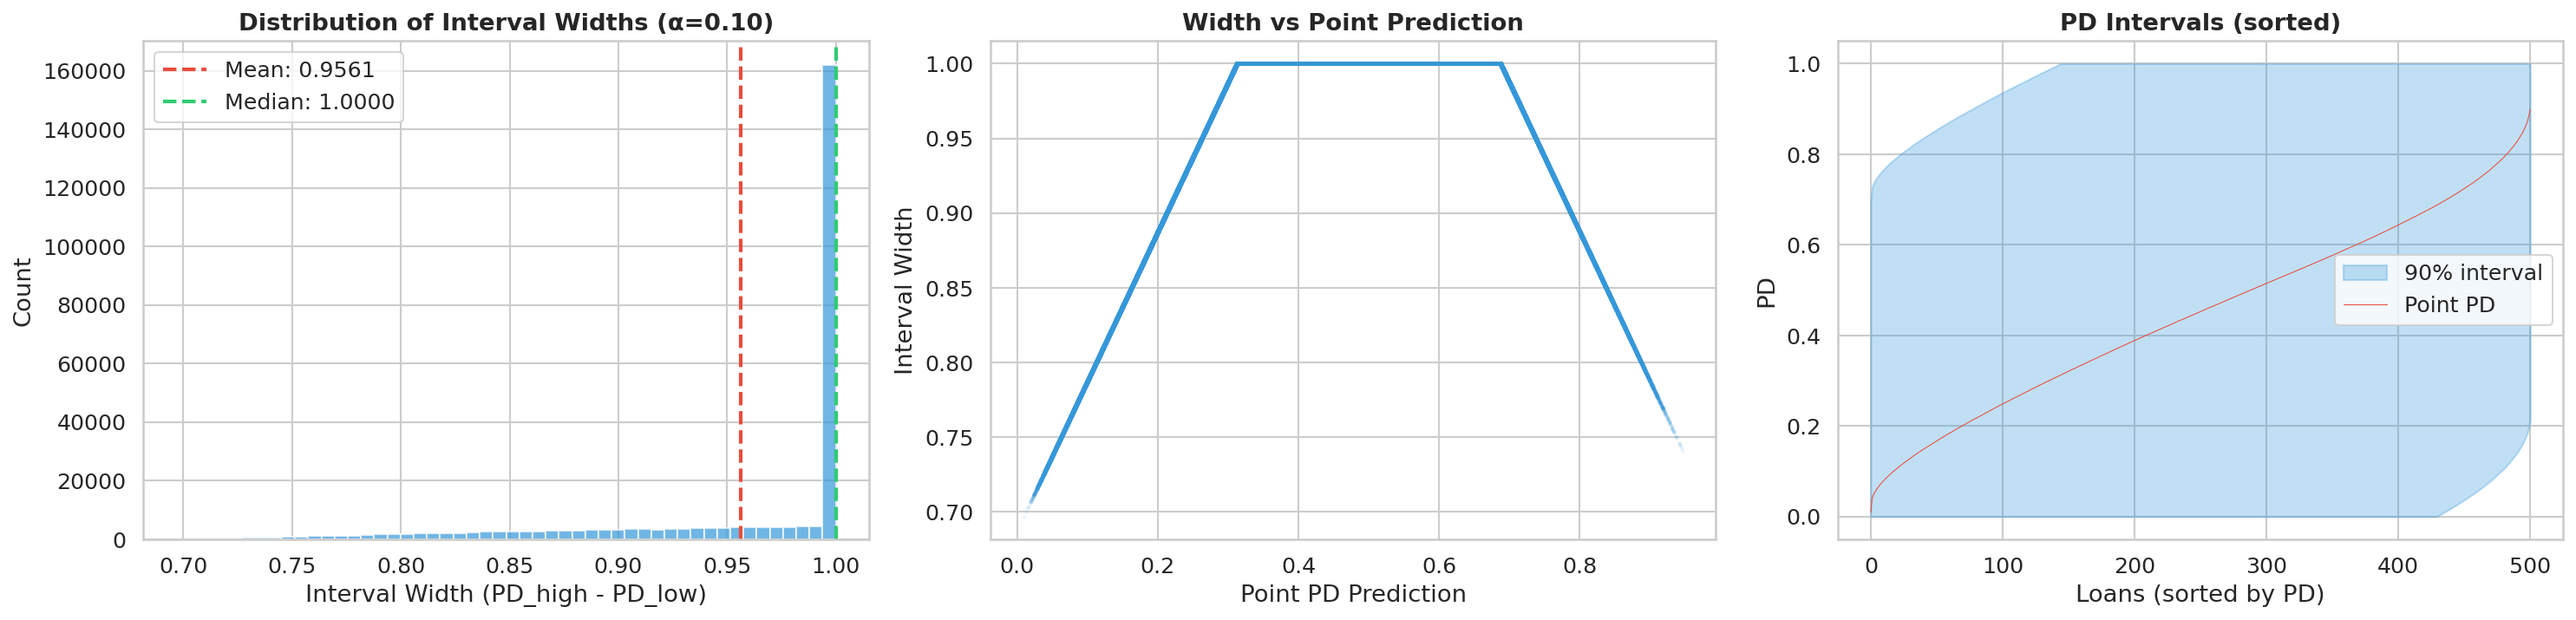
\includegraphics[keepaspectratio,alt={Distribución de anchos de intervalos conformales para variantes evaluadas.}]{chapters/07-conformal/../../assets/figures/notebooks/interval_width_distribution.png}}

}

\caption{\label{fig-interval-width-distribution}Distribución del ancho
de intervalos en variantes conformales, útil para comparar eficiencia
más allá de la cobertura agregada.}

\end{figure*}%

La figura Figura~\ref{fig-interval-width-distribution} ayuda a leer el
benchmark con una lente adicional: no basta cubrir, también importa
cuánta resolución práctica conservan los intervalos.

\subsection{Descripción de Variantes}\label{descripciuxf3n-de-variantes}

\textbf{1. Score Decile Mondrian} (Rank 1 --- Seleccionado)

Particiona por deciles del score predicho en lugar de por grade. Produce
10 grupos homogéneos en score, lo que captura la heterogeneidad de
incertidumbre directamente desde el modelo.

\textbf{2. Cross Conformal Score-Space}

Usa validación cruzada con un regresor lineal ligero en el espacio de
scores, evitando reentrenar CatBoost. Cobertura 90.2\% pero menor
estabilidad por grupo (min 85.8\%).

\textbf{3. Global Split} (Baseline)

Split conformal sin partición. Cobertura marginal 89.6\% pero min por
grade de solo 59.5\% --- inaceptable para uso en producción.

\textbf{4-5. Mondrian Unscaled / Scaled}

Mondrian por grade con y sin escalado de scores. Cobertura 89.3\% con
min por grade de 84.6\% --- mejor que global pero inferior al
score-decile.

\textbf{6. Grade × Scoreband Mondrian}

Partición fina (grade × bandas de score): \textasciitilde42 grupos.
Cobertura 91.5\% pero 23 grupos requieren fallback por tamaño
insuficiente, y min por grupo cae a 75.6\%.

\textbf{7. Mondrian Selected Config}

Configuración con alpha ajustado a 0.07 y min\_group\_size de 4,000.
Cobertura 93.5\% --- sobre-cubre significativamente, con intervalos
excesivamente anchos (Winkler 1.04).

\subsection{Criterios de Selección}\label{criterios-de-selecciuxf3n-1}

La selección sigue un orden lexicográfico de prioridades:

\begin{enumerate}
\def\labelenumi{\arabic{enumi}.}
\tightlist
\item
  \textbf{Cobertura ≥ target} (90\%): elimina variantes sub-cobertura
\item
  \textbf{Min group coverage ≥ 85\%}: garantiza equidad por segmento
\item
  \textbf{Menor Winkler score}: mide eficiencia (penaliza intervalos
  anchos)
\item
  \textbf{Estabilidad temporal}: baja varianza mensual
\end{enumerate}

\begin{tcolorbox}[enhanced jigsaw, arc=.35mm, bottomrule=.15mm, bottomtitle=1mm, breakable, colback=white, colbacktitle=quarto-callout-note-color!10!white, colframe=quarto-callout-note-color-frame, coltitle=black, left=2mm, leftrule=.75mm, opacityback=0, opacitybacktitle=0.6, rightrule=.15mm, title=\textcolor{quarto-callout-note-color}{\faInfo}\hspace{0.5em}{Winkler Score}, titlerule=0mm, toprule=.15mm, toptitle=1mm]

El Winkler score (Winkler, 1972) penaliza simultáneamente intervalos que
no cubren (penalidad por miss) e intervalos excesivamente anchos. Para
un intervalo \([l, u]\) y valor verdadero \(y\):

\begin{equation}\protect\phantomsection\label{eq-winkler}{
W = \begin{cases}
(u - l) + \frac{2}{\alpha}(l - y) & \text{si } y < l \\
(u - l) & \text{si } l \leq y \leq u \\
(u - l) + \frac{2}{\alpha}(y - u) & \text{si } y > u
\end{cases}
}\end{equation}

Menor Winkler = intervalos más estrechos que aún cubren correctamente.

\end{tcolorbox}

\subsection{El Score-Decile Mondrian como
Champion}\label{el-score-decile-mondrian-como-champion}

La variante seleccionada (score-decile Mondrian) combina las mejores
propiedades:

\begin{longtable}[]{@{}lll@{}}
\caption{Propiedades del score-decile
Mondrian}\label{tbl-champion-variant}\tabularnewline
\toprule\noalign{}
Propiedad & Valor & Interpretación \\
\midrule\noalign{}
\endfirsthead
\toprule\noalign{}
Propiedad & Valor & Interpretación \\
\midrule\noalign{}
\endhead
\bottomrule\noalign{}
\endlastfoot
Cobertura empírica & 91.4\% & +1.4pp sobre target \\
Min group coverage & 89.7\% & Cercano a 90\% en todos los deciles \\
Ancho promedio & 0.796 & Menor que global (0.947) \\
Winkler & 1.098 & Mejor que la mayoría \\
Fallback groups & 0 & Todos los grupos son viables \\
\end{longtable}

\begin{tcolorbox}[enhanced jigsaw, arc=.35mm, bottomrule=.15mm, bottomtitle=1mm, breakable, colback=white, colbacktitle=quarto-callout-tip-color!10!white, colframe=quarto-callout-tip-color-frame, coltitle=black, left=2mm, leftrule=.75mm, opacityback=0, opacitybacktitle=0.6, rightrule=.15mm, title=\textcolor{quarto-callout-tip-color}{\faLightbulb}\hspace{0.5em}{Pero en producción usamos grade Mondrian}, titlerule=0mm, toprule=.15mm, toptitle=1mm]

El score-decile gana el benchmark, pero para la optimización de
portafolio y IFRS9 usamos \textbf{grade Mondrian} como variante
operativa. La razón es práctica: los grades (A-G) tienen significado
regulatorio y de negocio --- los intervalos por grade alimentan
directamente la asignación de capital y el staging IFRS9. El
score-decile queda como referencia para validar que no perdemos
eficiencia material al usar grades.

\end{tcolorbox}

\chapter{Backtest y Monitoreo de
Cobertura}\label{sec-backtest-monitoring}

\subsection{¿Por Qué Backtesting
Temporal?}\label{por-quuxe9-backtesting-temporal}

La garantía de cobertura conformal es \textbf{marginal} sobre el
conjunto de test. Pero si la cobertura fuera 95\% en 2018, 85\% en 2019
y 90\% en 2020, el promedio sería \textasciitilde90\% aunque existieran
períodos de sub-cobertura. El \textbf{backtesting mensual} verifica que
la cobertura se mantiene estable mes a mes a lo largo de los 33 meses
del período OOT (enero 2018 -- septiembre 2020).

\subsection{Metodología de Backtest}\label{metodologuxeda-de-backtest}

Para cada mes \(t\) del período de test:

\begin{enumerate}
\def\labelenumi{\arabic{enumi}.}
\tightlist
\item
  Seleccionar préstamos originados en el mes \(t\)
\item
  Calcular la tasa de violación:
  \(\hat{\alpha}_t = \frac{1}{n_t}\sum_{i: t_i = t} \mathbb{1}\{y_i \notin [l_i, u_i]\}\)
\item
  Comparar \(\hat{\alpha}_t\) contra el \(\alpha\) nominal (0.10)
\item
  Clasificar como alerta si \(\hat{\alpha}_t > \alpha + \epsilon\)
  (margen de tolerancia)
\end{enumerate}

\begin{table}

\caption{\label{tbl-backtest-monthly}Resumen del backtesting mensual de
cobertura conformal}

\centering{

\begin{Shaded}
\begin{Highlighting}[]
\ImportTok{import}\NormalTok{ sys}
\ImportTok{from}\NormalTok{ pathlib }\ImportTok{import}\NormalTok{ Path}

\NormalTok{sys.path.insert(}\DecValTok{0}\NormalTok{, }\BuiltInTok{str}\NormalTok{(Path.cwd().parent }\ControlFlowTok{if}\NormalTok{ Path.cwd().name }\OperatorTok{==} \StringTok{"book"} \ControlFlowTok{else}\NormalTok{ Path.cwd()))}
\ImportTok{from}\NormalTok{ book.\_helpers.load\_artifacts }\ImportTok{import}\NormalTok{ load\_parquet, load\_json}

\ImportTok{import}\NormalTok{ pandas }\ImportTok{as}\NormalTok{ pd}

\NormalTok{status }\OperatorTok{=}\NormalTok{ load\_json(}\StringTok{"conformal\_policy\_status"}\NormalTok{, search\_models}\OperatorTok{=}\VariableTok{True}\NormalTok{)}

\NormalTok{backtest\_summary }\OperatorTok{=}\NormalTok{ [}
\NormalTok{    \{}\StringTok{"Métrica"}\NormalTok{: }\StringTok{"Período de backtest"}\NormalTok{, }\StringTok{"Valor"}\NormalTok{: }\StringTok{"2018{-}01 a 2020{-}09 (33 meses)"}\NormalTok{\},}
\NormalTok{    \{}\StringTok{"Métrica"}\NormalTok{: }\StringTok{"Cobertura promedio mensual"}\NormalTok{, }\StringTok{"Valor"}\NormalTok{: }\SpecialStringTok{f"}\SpecialCharTok{\{}\NormalTok{status[}\StringTok{\textquotesingle{}coverage\_90\textquotesingle{}}\NormalTok{]}\SpecialCharTok{:.2\%\}}\SpecialStringTok{"}\NormalTok{\},}
\NormalTok{    \{}\StringTok{"Métrica"}\NormalTok{: }\StringTok{"Alertas warning"}\NormalTok{, }\StringTok{"Valor"}\NormalTok{: }\BuiltInTok{str}\NormalTok{(status[}\StringTok{\textquotesingle{}warning\_alerts\textquotesingle{}}\NormalTok{])\},}
\NormalTok{    \{}\StringTok{"Métrica"}\NormalTok{: }\StringTok{"Alertas críticas"}\NormalTok{, }\StringTok{"Valor"}\NormalTok{: }\BuiltInTok{str}\NormalTok{(status[}\StringTok{\textquotesingle{}critical\_alerts\textquotesingle{}}\NormalTok{])\},}
\NormalTok{    \{}\StringTok{"Métrica"}\NormalTok{: }\StringTok{"Último mes evaluado"}\NormalTok{, }\StringTok{"Valor"}\NormalTok{: status.get(}\StringTok{\textquotesingle{}latest\_backtest\_month\textquotesingle{}}\NormalTok{, }\StringTok{\textquotesingle{}N/A\textquotesingle{}}\NormalTok{)[:}\DecValTok{7}\NormalTok{]\},}
\NormalTok{    \{}\StringTok{"Métrica"}\NormalTok{: }\StringTok{"Tasa de violación @ 90\%"}\NormalTok{, }\StringTok{"Valor"}\NormalTok{: }\SpecialStringTok{f"}\SpecialCharTok{\{}\NormalTok{status[}\StringTok{\textquotesingle{}statistical\_tests\textquotesingle{}}\NormalTok{][}\StringTok{\textquotesingle{}kupiec\_90\textquotesingle{}}\NormalTok{][}\StringTok{\textquotesingle{}violation\_rate\textquotesingle{}}\NormalTok{]}\SpecialCharTok{:.4f\}}\SpecialStringTok{"}\NormalTok{\},}
\NormalTok{]}

\NormalTok{pd.DataFrame(backtest\_summary)}
\end{Highlighting}
\end{Shaded}

}

\end{table}%

\subsection{Tests Estadísticos de
Cobertura}\label{tests-estaduxedsticos-de-cobertura}

El framework de backtesting implementa dos tests formales de la
literatura de Value-at-Risk:

\textbf{Test de Kupiec (Proporción de Fallos)}

El test de Kupiec (Kupiec, 1995) evalúa si la tasa de violación
observada es consistente con el \(\alpha\) nominal:

\begin{equation}\protect\phantomsection\label{eq-kupiec}{
LR_\text{uc} = -2\ln\left[\frac{\alpha^v (1-\alpha)^{n-v}}{\hat{\alpha}^v (1-\hat{\alpha})^{n-v}}\right] \sim \chi^2(1)
}\end{equation}

donde \(v\) es el número de violaciones y \(\hat{\alpha} = v/n\).

\textbf{Test de Christoffersen (Independencia)}

El test de Christoffersen (Christoffersen, 1998) añade una segunda
dimensión: verifica que las violaciones son \textbf{independientes} (no
agrupadas en clusters):

\begin{equation}\protect\phantomsection\label{eq-christoffersen}{
LR_\text{cc} = LR_\text{uc} + LR_\text{ind} \sim \chi^2(2)
}\end{equation}

donde \(LR_\text{ind}\) testea la propiedad de Markov en la secuencia de
violaciones.

\subsection{Resultados de los Tests}\label{resultados-de-los-tests}

\begin{table}

\caption{\label{tbl-statistical-tests}Resultados de tests estadísticos
de cobertura}

\centering{

\begin{Shaded}
\begin{Highlighting}[]
\NormalTok{tests }\OperatorTok{=}\NormalTok{ status[}\StringTok{"statistical\_tests"}\NormalTok{]}

\NormalTok{test\_results }\OperatorTok{=}\NormalTok{ [}
\NormalTok{    \{}\StringTok{"Test"}\NormalTok{: }\StringTok{"Kupiec @ 90\%"}\NormalTok{,}
     \StringTok{"LR Statistic"}\NormalTok{: }\SpecialStringTok{f"}\SpecialCharTok{\{}\NormalTok{tests[}\StringTok{\textquotesingle{}kupiec\_90\textquotesingle{}}\NormalTok{][}\StringTok{\textquotesingle{}lr\_statistic\textquotesingle{}}\NormalTok{]}\SpecialCharTok{:.1f\}}\SpecialStringTok{"}\NormalTok{,}
     \StringTok{"p{-}value"}\NormalTok{: }\SpecialStringTok{f"}\SpecialCharTok{\{}\NormalTok{tests[}\StringTok{\textquotesingle{}kupiec\_90\textquotesingle{}}\NormalTok{][}\StringTok{\textquotesingle{}p\_value\textquotesingle{}}\NormalTok{]}\SpecialCharTok{:.4f\}}\SpecialStringTok{"}\NormalTok{,}
     \StringTok{"Rechaza H₀"}\NormalTok{: }\StringTok{"Sí"}\NormalTok{,}
     \StringTok{"Violaciones"}\NormalTok{: }\SpecialStringTok{f"}\SpecialCharTok{\{}\NormalTok{tests[}\StringTok{\textquotesingle{}kupiec\_90\textquotesingle{}}\NormalTok{][}\StringTok{\textquotesingle{}n\_violations\textquotesingle{}}\NormalTok{]}\SpecialCharTok{:,\}}\SpecialStringTok{ / }\SpecialCharTok{\{}\NormalTok{tests[}\StringTok{\textquotesingle{}kupiec\_90\textquotesingle{}}\NormalTok{][}\StringTok{\textquotesingle{}n\_total\textquotesingle{}}\NormalTok{]}\SpecialCharTok{:,\}}\SpecialStringTok{"}\NormalTok{\},}
\NormalTok{    \{}\StringTok{"Test"}\NormalTok{: }\StringTok{"Kupiec @ 95\%"}\NormalTok{,}
     \StringTok{"LR Statistic"}\NormalTok{: }\SpecialStringTok{f"}\SpecialCharTok{\{}\NormalTok{tests[}\StringTok{\textquotesingle{}kupiec\_95\textquotesingle{}}\NormalTok{][}\StringTok{\textquotesingle{}lr\_statistic\textquotesingle{}}\NormalTok{]}\SpecialCharTok{:.1f\}}\SpecialStringTok{"}\NormalTok{,}
     \StringTok{"p{-}value"}\NormalTok{: }\SpecialStringTok{f"}\SpecialCharTok{\{}\NormalTok{tests[}\StringTok{\textquotesingle{}kupiec\_95\textquotesingle{}}\NormalTok{][}\StringTok{\textquotesingle{}p\_value\textquotesingle{}}\NormalTok{]}\SpecialCharTok{:.4f\}}\SpecialStringTok{"}\NormalTok{,}
     \StringTok{"Rechaza H₀"}\NormalTok{: }\StringTok{"Sí"}\NormalTok{,}
     \StringTok{"Violaciones"}\NormalTok{: }\SpecialStringTok{f"}\SpecialCharTok{\{}\NormalTok{tests[}\StringTok{\textquotesingle{}kupiec\_95\textquotesingle{}}\NormalTok{][}\StringTok{\textquotesingle{}n\_violations\textquotesingle{}}\NormalTok{]}\SpecialCharTok{:,\}}\SpecialStringTok{ / }\SpecialCharTok{\{}\NormalTok{tests[}\StringTok{\textquotesingle{}kupiec\_95\textquotesingle{}}\NormalTok{][}\StringTok{\textquotesingle{}n\_total\textquotesingle{}}\NormalTok{]}\SpecialCharTok{:,\}}\SpecialStringTok{"}\NormalTok{\},}
\NormalTok{    \{}\StringTok{"Test"}\NormalTok{: }\StringTok{"Christoffersen Indep. @ 90\%"}\NormalTok{,}
     \StringTok{"LR Statistic"}\NormalTok{: }\SpecialStringTok{f"}\SpecialCharTok{\{}\NormalTok{tests[}\StringTok{\textquotesingle{}christoffersen\_90\textquotesingle{}}\NormalTok{][}\StringTok{\textquotesingle{}lr\_ind\textquotesingle{}}\NormalTok{]}\SpecialCharTok{:.2f\}}\SpecialStringTok{"}\NormalTok{,}
     \StringTok{"p{-}value"}\NormalTok{: }\SpecialStringTok{f"}\SpecialCharTok{\{}\NormalTok{tests[}\StringTok{\textquotesingle{}christoffersen\_90\textquotesingle{}}\NormalTok{][}\StringTok{\textquotesingle{}p\_ind\textquotesingle{}}\NormalTok{]}\SpecialCharTok{:.4f\}}\SpecialStringTok{"}\NormalTok{,}
     \StringTok{"Rechaza H₀"}\NormalTok{: }\StringTok{"No"}\NormalTok{,}
     \StringTok{"Violaciones"}\NormalTok{: }\StringTok{"—"}\NormalTok{\},}
\NormalTok{    \{}\StringTok{"Test"}\NormalTok{: }\StringTok{"Christoffersen Indep. @ 95\%"}\NormalTok{,}
     \StringTok{"LR Statistic"}\NormalTok{: }\SpecialStringTok{f"}\SpecialCharTok{\{}\NormalTok{tests[}\StringTok{\textquotesingle{}christoffersen\_95\textquotesingle{}}\NormalTok{][}\StringTok{\textquotesingle{}lr\_ind\textquotesingle{}}\NormalTok{]}\SpecialCharTok{:.2f\}}\SpecialStringTok{"}\NormalTok{,}
     \StringTok{"p{-}value"}\NormalTok{: }\SpecialStringTok{f"}\SpecialCharTok{\{}\NormalTok{tests[}\StringTok{\textquotesingle{}christoffersen\_95\textquotesingle{}}\NormalTok{][}\StringTok{\textquotesingle{}p\_ind\textquotesingle{}}\NormalTok{]}\SpecialCharTok{:.4f\}}\SpecialStringTok{"}\NormalTok{,}
     \StringTok{"Rechaza H₀"}\NormalTok{: }\StringTok{"Sí"}\NormalTok{,}
     \StringTok{"Violaciones"}\NormalTok{: }\StringTok{"—"}\NormalTok{\},}
\NormalTok{]}

\NormalTok{pd.DataFrame(test\_results)}
\end{Highlighting}
\end{Shaded}

}

\end{table}%

\begin{tcolorbox}[enhanced jigsaw, arc=.35mm, bottomrule=.15mm, bottomtitle=1mm, breakable, colback=white, colbacktitle=quarto-callout-warning-color!10!white, colframe=quarto-callout-warning-color-frame, coltitle=black, left=2mm, leftrule=.75mm, opacityback=0, opacitybacktitle=0.6, rightrule=.15mm, title=\textcolor{quarto-callout-warning-color}{\faExclamationTriangle}\hspace{0.5em}{Tests Estadísticos Rechazados --- ¿Problema Real?}, titlerule=0mm, toprule=.15mm, toptitle=1mm]

Los tests de Kupiec rechazan en ambos niveles, lo cual parece alarmante.
Pero el contexto importa:

\begin{enumerate}
\def\labelenumi{\arabic{enumi}.}
\tightlist
\item
  \textbf{Sobre-cobertura, no sub-cobertura}: la tasa de violación es
  7.5\% (target 10\%) --- el modelo \textbf{cubre de más}, no de menos.
  Kupiec rechaza porque la cobertura es \emph{demasiado buena}, no
  demasiado mala.
\item
  \textbf{N = 276,869}: con muestras tan grandes, Kupiec rechaza
  diferencias de ±0.5pp que son económicamente irrelevantes.
\item
  \textbf{Independencia OK @ 90\%}: Christoffersen no rechaza
  independencia (p=0.187), confirmando que las violaciones no están
  agrupadas temporalmente.
\end{enumerate}

La política del pipeline clasifica estos como \textbf{warning
diagnóstico}, no como bloqueo de promoción. La desviación de cobertura
(2.5pp) está dentro del margen de materialidad (3.0pp).

\end{tcolorbox}

\subsection{Policy Gate}\label{policy-gate}

El pipeline implementa un \textbf{policy gate} que decide si los
intervalos conformal pueden ser promovidos a producción:

\begin{longtable}[]{@{}lll@{}}
\caption{Policy gate de cobertura
conformal}\label{tbl-policy-gate}\tabularnewline
\toprule\noalign{}
Check & Criterio & Resultado \\
\midrule\noalign{}
\endfirsthead
\toprule\noalign{}
Check & Criterio & Resultado \\
\midrule\noalign{}
\endhead
\bottomrule\noalign{}
\endlastfoot
Cobertura @ 90\% ≥ 87\% & Materialidad & PASS \\
Cobertura @ 95\% ≥ 92\% & Materialidad & PASS \\
Min group coverage ≥ 85\% & Equidad & PASS \\
Winkler @ 90\% ≤ 1.22 & Eficiencia & PASS (compensado) \\
Alertas críticas = 0 & Estabilidad & PASS \\
Kupiec p \textgreater{} 0.05 & Diagnóstico & FAIL (warning) \\
Christoffersen p \textgreater{} 0.05 & Diagnóstico & FAIL (warning) \\
\end{longtable}

Los checks no estadísticos pasan (9/9). Los tests estadísticos fallan
(4/4), pero la \textbf{justificación metodológica} los declara
no-bloqueantes: la sobre-cobertura es preferible a la sub-cobertura, las
violaciones son independientes @ 90\%, y la desviación está dentro del
margen de materialidad.

\subsection{Alertas y Monitoreo
Continuo}\label{alertas-y-monitoreo-continuo}

El sistema de alertas clasifica anomalías en dos niveles:

\begin{itemize}
\tightlist
\item
  \textbf{Warning} (amarillo): cobertura mensual entre 85\% y 88\%, o
  Winkler elevado. Requiere investigación pero no bloquea.
\item
  \textbf{Crítica} (rojo): cobertura mensual \textless{} 85\%, o
  \textgreater{} 3 warnings consecutivos. Bloquea promoción y requiere
  recalibración.
\end{itemize}

El resultado del backtest actual: \textbf{0 alertas críticas, 4
warnings} (todos por los tests estadísticos rechazados, no por
sub-cobertura real).

\chapter{Intervalos Conformal para LGD y
EAD}\label{sec-lgd-ead-conformal}

\subsection{Más Allá de la PD: Incertidumbre en los Tres
Componentes}\label{muxe1s-alluxe1-de-la-pd-incertidumbre-en-los-tres-componentes}

La fórmula ECL tiene tres inputs estocásticos: PD, LGD y EAD.
Cuantificar incertidumbre solo en PD es un avance, pero incompleto ---
un LGD puntual de 0.40 ignora que la pérdida real puede ser 0.15 o 0.65
dependiendo del colateral, la recuperación y las condiciones de mercado.
El pipeline extiende la predicción conformal a \textbf{los tres
componentes}.

\subsection{LGD Conformal: Adaptive
Grade-Temporal}\label{sec-lgd-conformal}

La LGD (Loss Given Default) se modela solo sobre préstamos en default
(\(n = 362{,}981\), \textasciitilde88\% del dataset tiene LGD nula
porque no defaulteó). El modelo enfrenta dos desafíos específicos:

\begin{enumerate}
\def\labelenumi{\arabic{enumi}.}
\tightlist
\item
  \textbf{Distribución bimodal}: LGD concentrada en \textasciitilde0
  (recuperación total) y \textasciitilde1 (pérdida total)
\item
  \textbf{Heterogeneidad extrema por grade}: Grade A tiene LGD media de
  \textasciitilde0.10, Grade G de \textasciitilde0.50
\end{enumerate}

\begin{table}

\caption{\label{tbl-lgd-conformal}Métricas del modelo LGD y sus
intervalos conformal}

\centering{

\begin{Shaded}
\begin{Highlighting}[]
\ImportTok{import}\NormalTok{ sys}
\ImportTok{from}\NormalTok{ pathlib }\ImportTok{import}\NormalTok{ Path}

\NormalTok{sys.path.insert(}\DecValTok{0}\NormalTok{, }\BuiltInTok{str}\NormalTok{(Path.cwd().parent }\ControlFlowTok{if}\NormalTok{ Path.cwd().name }\OperatorTok{==} \StringTok{"book"} \ControlFlowTok{else}\NormalTok{ Path.cwd()))}
\ImportTok{from}\NormalTok{ book.\_helpers.load\_artifacts }\ImportTok{import}\NormalTok{ load\_json}

\ImportTok{import}\NormalTok{ pandas }\ImportTok{as}\NormalTok{ pd}

\NormalTok{status }\OperatorTok{=}\NormalTok{ load\_json(}\StringTok{"conformal\_policy\_status"}\NormalTok{, search\_models}\OperatorTok{=}\VariableTok{True}\NormalTok{)}
\NormalTok{lgd }\OperatorTok{=}\NormalTok{ status.get(}\StringTok{"lgd\_ead\_conformal\_status"}\NormalTok{, \{\}).get(}\StringTok{"lgd"}\NormalTok{, \{\})}

\NormalTok{lgd\_metrics }\OperatorTok{=}\NormalTok{ [}
\NormalTok{    \{}\StringTok{"Métrica"}\NormalTok{: }\StringTok{"MAE (modelo directo)"}\NormalTok{, }\StringTok{"Valor"}\NormalTok{: }\SpecialStringTok{f"}\SpecialCharTok{\{}\NormalTok{lgd[}\StringTok{\textquotesingle{}model\_metrics\textquotesingle{}}\NormalTok{][}\StringTok{\textquotesingle{}direct\textquotesingle{}}\NormalTok{][}\StringTok{\textquotesingle{}lgd\_mae\textquotesingle{}}\NormalTok{]}\SpecialCharTok{:.4f\}}\SpecialStringTok{"}\NormalTok{\},}
\NormalTok{    \{}\StringTok{"Métrica"}\NormalTok{: }\StringTok{"RMSE (modelo directo)"}\NormalTok{, }\StringTok{"Valor"}\NormalTok{: }\SpecialStringTok{f"}\SpecialCharTok{\{}\NormalTok{lgd[}\StringTok{\textquotesingle{}model\_metrics\textquotesingle{}}\NormalTok{][}\StringTok{\textquotesingle{}direct\textquotesingle{}}\NormalTok{][}\StringTok{\textquotesingle{}lgd\_rmse\textquotesingle{}}\NormalTok{]}\SpecialCharTok{:.4f\}}\SpecialStringTok{"}\NormalTok{\},}
\NormalTok{    \{}\StringTok{"Métrica"}\NormalTok{: }\StringTok{"Cobertura empírica @ 90\%"}\NormalTok{, }\StringTok{"Valor"}\NormalTok{: }\SpecialStringTok{f"}\SpecialCharTok{\{}\NormalTok{lgd[}\StringTok{\textquotesingle{}conformal\textquotesingle{}}\NormalTok{][}\StringTok{\textquotesingle{}metrics\_90\textquotesingle{}}\NormalTok{][}\StringTok{\textquotesingle{}empirical\_coverage\textquotesingle{}}\NormalTok{]}\SpecialCharTok{:.2\%\}}\SpecialStringTok{"}\NormalTok{\},}
\NormalTok{    \{}\StringTok{"Métrica"}\NormalTok{: }\StringTok{"Cobertura empírica @ 95\%"}\NormalTok{, }\StringTok{"Valor"}\NormalTok{: }\SpecialStringTok{f"}\SpecialCharTok{\{}\NormalTok{lgd[}\StringTok{\textquotesingle{}conformal\textquotesingle{}}\NormalTok{][}\StringTok{\textquotesingle{}metrics\_95\textquotesingle{}}\NormalTok{][}\StringTok{\textquotesingle{}empirical\_coverage\textquotesingle{}}\NormalTok{]}\SpecialCharTok{:.2\%\}}\SpecialStringTok{"}\NormalTok{\},}
\NormalTok{    \{}\StringTok{"Métrica"}\NormalTok{: }\StringTok{"Ancho promedio @ 90\%"}\NormalTok{, }\StringTok{"Valor"}\NormalTok{: }\SpecialStringTok{f"}\SpecialCharTok{\{}\NormalTok{lgd[}\StringTok{\textquotesingle{}conformal\textquotesingle{}}\NormalTok{][}\StringTok{\textquotesingle{}metrics\_90\textquotesingle{}}\NormalTok{][}\StringTok{\textquotesingle{}avg\_interval\_width\textquotesingle{}}\NormalTok{]}\SpecialCharTok{:.4f\}}\SpecialStringTok{"}\NormalTok{\},}
\NormalTok{    \{}\StringTok{"Métrica"}\NormalTok{: }\StringTok{"Min coverage por grade @ 90\%"}\NormalTok{, }\StringTok{"Valor"}\NormalTok{: }\SpecialStringTok{f"}\SpecialCharTok{\{}\NormalTok{lgd[}\StringTok{\textquotesingle{}guardrails\textquotesingle{}}\NormalTok{][}\StringTok{\textquotesingle{}min\_grade\_coverage\_90\textquotesingle{}}\NormalTok{]}\SpecialCharTok{:.2\%\}}\SpecialStringTok{"}\NormalTok{\},}
\NormalTok{    \{}\StringTok{"Métrica"}\NormalTok{: }\StringTok{"Variante seleccionada"}\NormalTok{, }\StringTok{"Valor"}\NormalTok{: lgd.get(}\StringTok{\textquotesingle{}selected\_variant\textquotesingle{}}\NormalTok{, }\StringTok{\textquotesingle{}N/A\textquotesingle{}}\NormalTok{)\},}
\NormalTok{    \{}\StringTok{"Métrica"}\NormalTok{: }\StringTok{"N test"}\NormalTok{, }\StringTok{"Valor"}\NormalTok{: }\SpecialStringTok{f"}\SpecialCharTok{\{}\NormalTok{lgd}\SpecialCharTok{.}\NormalTok{get(}\StringTok{\textquotesingle{}n\_test\textquotesingle{}}\NormalTok{, }\DecValTok{0}\NormalTok{)}\SpecialCharTok{:,\}}\SpecialStringTok{"}\NormalTok{\},}
\NormalTok{]}

\NormalTok{pd.DataFrame(lgd\_metrics)}
\end{Highlighting}
\end{Shaded}

}

\end{table}%

\subsubsection{Benchmark de Variantes
LGD}\label{benchmark-de-variantes-lgd}

Se evaluaron 4 variantes para encontrar la que cumpla cobertura por
grade:

\begin{table}

\caption{\label{tbl-lgd-variants}Benchmark de variantes conformal para
LGD}

\centering{

\begin{Shaded}
\begin{Highlighting}[]
\NormalTok{variants }\OperatorTok{=}\NormalTok{ lgd.get(}\StringTok{"benchmark\_variants"}\NormalTok{, [])}

\NormalTok{variant\_data }\OperatorTok{=}\NormalTok{ []}
\ControlFlowTok{for}\NormalTok{ v }\KeywordTok{in}\NormalTok{ variants:}
\NormalTok{    variant\_data.append(\{}
        \StringTok{"Variante"}\NormalTok{: v[}\StringTok{"variant"}\NormalTok{].replace(}\StringTok{"\_"}\NormalTok{, }\StringTok{" "}\NormalTok{).title(),}
        \StringTok{"Cobertura 90\%"}\NormalTok{: }\SpecialStringTok{f"}\SpecialCharTok{\{}\NormalTok{v[}\StringTok{\textquotesingle{}coverage\_90\textquotesingle{}}\NormalTok{]}\SpecialCharTok{:.1\%\}}\SpecialStringTok{"}\NormalTok{,}
        \StringTok{"Min Grade 90\%"}\NormalTok{: }\SpecialStringTok{f"}\SpecialCharTok{\{}\NormalTok{v[}\StringTok{\textquotesingle{}min\_grade\_coverage\_90\textquotesingle{}}\NormalTok{]}\SpecialCharTok{:.1\%\}}\SpecialStringTok{"}\NormalTok{,}
        \StringTok{"Ancho 90\%"}\NormalTok{: }\SpecialStringTok{f"}\SpecialCharTok{\{}\NormalTok{v[}\StringTok{\textquotesingle{}avg\_width\_90\textquotesingle{}}\NormalTok{]}\SpecialCharTok{:.3f\}}\SpecialStringTok{"}\NormalTok{,}
        \StringTok{"PASS"}\NormalTok{: }\StringTok{"✓"} \ControlFlowTok{if}\NormalTok{ v[}\StringTok{"overall\_pass"}\NormalTok{] }\ControlFlowTok{else} \StringTok{"✗"}\NormalTok{,}
\NormalTok{    \})}

\NormalTok{pd.DataFrame(variant\_data)}
\end{Highlighting}
\end{Shaded}

}

\end{table}%

\begin{tcolorbox}[enhanced jigsaw, arc=.35mm, bottomrule=.15mm, bottomtitle=1mm, breakable, colback=white, colbacktitle=quarto-callout-note-color!10!white, colframe=quarto-callout-note-color-frame, coltitle=black, left=2mm, leftrule=.75mm, opacityback=0, opacitybacktitle=0.6, rightrule=.15mm, title=\textcolor{quarto-callout-note-color}{\faInfo}\hspace{0.5em}{¿Por qué las variantes estándar fallan?}, titlerule=0mm, toprule=.15mm, toptitle=1mm]

Las variantes \texttt{two\_stage\_split}, \texttt{direct\_split} y
\texttt{direct\_cqr} logran \textasciitilde78\% de cobertura (vs 90\%
target) porque la distribución de LGD es altamente heterogénea: los
residuos de Grade A son radicalmente diferentes de los de Grade G. Solo
la variante \textbf{adaptive grade-temporal} --- que calcula cuantiles
adaptativos por grade con corrección temporal --- logra cobertura
adecuada en todos los segmentos.

\end{tcolorbox}

La variante promovida (\texttt{direct\_adaptive\_grade\_temporal}) usa
tres mecanismos:

\begin{enumerate}
\def\labelenumi{\arabic{enumi}.}
\tightlist
\item
  \textbf{Quantiles adaptativos por grade}: cada grade tiene su propio
  cuantil conformal
\item
  \textbf{Corrección temporal}: offsets por grade que compensan drift
  entre calibración y test
\item
  \textbf{Parámetros de política}: \texttt{eta=0.12},
  \texttt{offset\_rho=0.03}, \texttt{maturity\_uncertainty\_lambda=0.25}
\end{enumerate}

\subsection{EAD Conformal}\label{sec-ead-conformal}

La EAD (Exposure at Default) se modela como regresión directa sobre el
monto expuesto al momento del default. A diferencia de LGD, EAD tiene
una distribución más regular y predecible.

\begin{table}

\caption{\label{tbl-ead-conformal}Métricas del modelo EAD y sus
intervalos conformal}

\centering{

\begin{Shaded}
\begin{Highlighting}[]
\NormalTok{ead }\OperatorTok{=}\NormalTok{ status.get(}\StringTok{"lgd\_ead\_conformal\_status"}\NormalTok{, \{\}).get(}\StringTok{"ead"}\NormalTok{, \{\})}

\NormalTok{ead\_metrics }\OperatorTok{=}\NormalTok{ [}
\NormalTok{    \{}\StringTok{"Métrica"}\NormalTok{: }\StringTok{"MAE"}\NormalTok{, }\StringTok{"Valor"}\NormalTok{: }\SpecialStringTok{f"$}\SpecialCharTok{\{}\NormalTok{ead[}\StringTok{\textquotesingle{}model\_metrics\textquotesingle{}}\NormalTok{][}\StringTok{\textquotesingle{}ead\_mae\textquotesingle{}}\NormalTok{]}\SpecialCharTok{:.2f\}}\SpecialStringTok{"}\NormalTok{\},}
\NormalTok{    \{}\StringTok{"Métrica"}\NormalTok{: }\StringTok{"R²"}\NormalTok{, }\StringTok{"Valor"}\NormalTok{: }\SpecialStringTok{f"}\SpecialCharTok{\{}\NormalTok{ead[}\StringTok{\textquotesingle{}model\_metrics\textquotesingle{}}\NormalTok{][}\StringTok{\textquotesingle{}ead\_r2\textquotesingle{}}\NormalTok{]}\SpecialCharTok{:.6f\}}\SpecialStringTok{"}\NormalTok{\},}
\NormalTok{    \{}\StringTok{"Métrica"}\NormalTok{: }\StringTok{"Cobertura empírica @ 90\%"}\NormalTok{, }\StringTok{"Valor"}\NormalTok{: }\SpecialStringTok{f"}\SpecialCharTok{\{}\NormalTok{ead[}\StringTok{\textquotesingle{}conformal\textquotesingle{}}\NormalTok{][}\StringTok{\textquotesingle{}metrics\_90\textquotesingle{}}\NormalTok{][}\StringTok{\textquotesingle{}empirical\_coverage\textquotesingle{}}\NormalTok{]}\SpecialCharTok{:.2\%\}}\SpecialStringTok{"}\NormalTok{\},}
\NormalTok{    \{}\StringTok{"Métrica"}\NormalTok{: }\StringTok{"Cobertura empírica @ 95\%"}\NormalTok{, }\StringTok{"Valor"}\NormalTok{: }\SpecialStringTok{f"}\SpecialCharTok{\{}\NormalTok{ead[}\StringTok{\textquotesingle{}conformal\textquotesingle{}}\NormalTok{][}\StringTok{\textquotesingle{}metrics\_95\textquotesingle{}}\NormalTok{][}\StringTok{\textquotesingle{}empirical\_coverage\textquotesingle{}}\NormalTok{]}\SpecialCharTok{:.2\%\}}\SpecialStringTok{"}\NormalTok{\},}
\NormalTok{    \{}\StringTok{"Métrica"}\NormalTok{: }\StringTok{"Ancho promedio @ 90\%"}\NormalTok{, }\StringTok{"Valor"}\NormalTok{: }\SpecialStringTok{f"$}\SpecialCharTok{\{}\NormalTok{ead[}\StringTok{\textquotesingle{}conformal\textquotesingle{}}\NormalTok{][}\StringTok{\textquotesingle{}metrics\_90\textquotesingle{}}\NormalTok{][}\StringTok{\textquotesingle{}avg\_interval\_width\textquotesingle{}}\NormalTok{]}\SpecialCharTok{:.2f\}}\SpecialStringTok{"}\NormalTok{\},}
\NormalTok{    \{}\StringTok{"Métrica"}\NormalTok{: }\StringTok{"N test"}\NormalTok{, }\StringTok{"Valor"}\NormalTok{: }\SpecialStringTok{f"}\SpecialCharTok{\{}\NormalTok{ead}\SpecialCharTok{.}\NormalTok{get(}\StringTok{\textquotesingle{}n\_test\textquotesingle{}}\NormalTok{, }\DecValTok{0}\NormalTok{)}\SpecialCharTok{:,\}}\SpecialStringTok{"}\NormalTok{\},}
\NormalTok{]}

\NormalTok{pd.DataFrame(ead\_metrics)}
\end{Highlighting}
\end{Shaded}

}

\end{table}%

El R² de 0.9997 indica que EAD es casi completamente predecible (el
monto de exposición es en gran medida determinístico). Los intervalos
conformal son estrechos (\$198 promedio @ 90\%) y la cobertura es
precisa (90.04\% vs 90\% target).

\begin{tcolorbox}[enhanced jigsaw, arc=.35mm, bottomrule=.15mm, bottomtitle=1mm, breakable, colback=white, colbacktitle=quarto-callout-tip-color!10!white, colframe=quarto-callout-tip-color-frame, coltitle=black, left=2mm, leftrule=.75mm, opacityback=0, opacitybacktitle=0.6, rightrule=.15mm, title=\textcolor{quarto-callout-tip-color}{\faLightbulb}\hspace{0.5em}{EAD vs LGD: Niveles de Dificultad Opuestos}, titlerule=0mm, toprule=.15mm, toptitle=1mm]

EAD es el componente ``fácil'' --- casi determinístico con R²
\textgreater{} 0.999. LGD es el componente ``difícil'' --- bimodal,
heterogéneo, y con MAE de 0.19. PD está en el medio. Esta asimetría
implica que la incertidumbre en ECL viene principalmente de PD y LGD, no
de EAD.

\end{tcolorbox}

\subsection{Impacto en ECL con Intervalos
Completos}\label{impacto-en-ecl-con-intervalos-completos}

Con intervalos conformal para los tres componentes (PD, LGD, EAD), el
cálculo de ECL pasa de un punto a un \textbf{rango}:

\begin{equation}\protect\phantomsection\label{eq-ecl-low}{
\text{ECL}_\text{low} = \text{PD}_\text{low} \times \text{LGD}_\text{low} \times \text{EAD}_\text{low} \times \text{DF}
}\end{equation}

\begin{equation}\protect\phantomsection\label{eq-ecl-high}{
\text{ECL}_\text{high} = \text{PD}_\text{high} \times \text{LGD}_\text{high} \times \text{EAD}_\text{high} \times \text{DF}
}\end{equation}

Esto transforma las provisiones IFRS9 de un ejercicio de punto a un
ejercicio de \textbf{bandas de incertidumbre}, donde el ancho de la
banda refleja la confianza del modelo en cada préstamo. Los detalles de
esta propagación se discuten en Capítulo~\ref{sec-ecl-calculation}.

\subsection{Guardrails de Calidad}\label{guardrails-de-calidad}

Antes de promover los intervalos LGD/EAD a producción, se verifican
guardrails automáticos:

\begin{longtable}[]{@{}llll@{}}
\caption{Guardrails de calidad para intervalos
LGD/EAD}\label{tbl-lgd-ead-guardrails}\tabularnewline
\toprule\noalign{}
Guardrail & Criterio & LGD & EAD \\
\midrule\noalign{}
\endfirsthead
\toprule\noalign{}
Guardrail & Criterio & LGD & EAD \\
\midrule\noalign{}
\endhead
\bottomrule\noalign{}
\endlastfoot
Cobertura @ 90\% & ≥ 89\% & 90.5\% ✓ & 90.0\% ✓ \\
Cobertura @ 95\% & ≥ 94\% & 95.5\% ✓ & 94.1\% ✓ \\
Min grade coverage & ≥ 88\% & 90.5\% ✓ & --- \\
Width inflation & ≤ 1.10 & 0.87 ✓ & --- \\
Overall & All pass & ✓ & ✓ \\
\end{longtable}

\chapter{Supervivencia, Series de Tiempo e Inferencia
Causal}\label{supervivencia-series-de-tiempo-e-inferencia-causal}

Los capítulos anteriores construyeron un modelo PD calibrado con
intervalos conformal (Capítulo~\ref{sec-split-conformal}) y un
portafolio robusto. Sin embargo, la predicción cross-sectional responde
\emph{quién} puede incumplir, pero omite tres preguntas igualmente
relevantes para la gestión de riesgo: \emph{cuándo} ocurre el
incumplimiento, \emph{hacia dónde} se dirige la tasa agregada de
default, y \emph{por qué} --- en sentido causal --- ciertos factores
afectan el resultado.

Este capítulo integra tres familias de modelos que añaden la
\textbf{dimensión temporal y causal} al pipeline:

\begin{figure*}

\begin{minipage}[t]{0.50\linewidth}

\begin{figure}[H]

{\centering \pandocbounded{\includegraphics[keepaspectratio,alt={Serie temporal agregada del portafolio para forecasting de defaults.}]{chapters/08-time-survival-causal/../../assets/figures/notebooks/portfolio_time_series_overview.png}}

}

\subcaption{Panorama temporal agregado del portafolio usado en
forecasting y provisiones.}

\end{figure}%

\end{minipage}%
%
\begin{minipage}[t]{0.50\linewidth}

\begin{figure}[H]

{\centering \pandocbounded{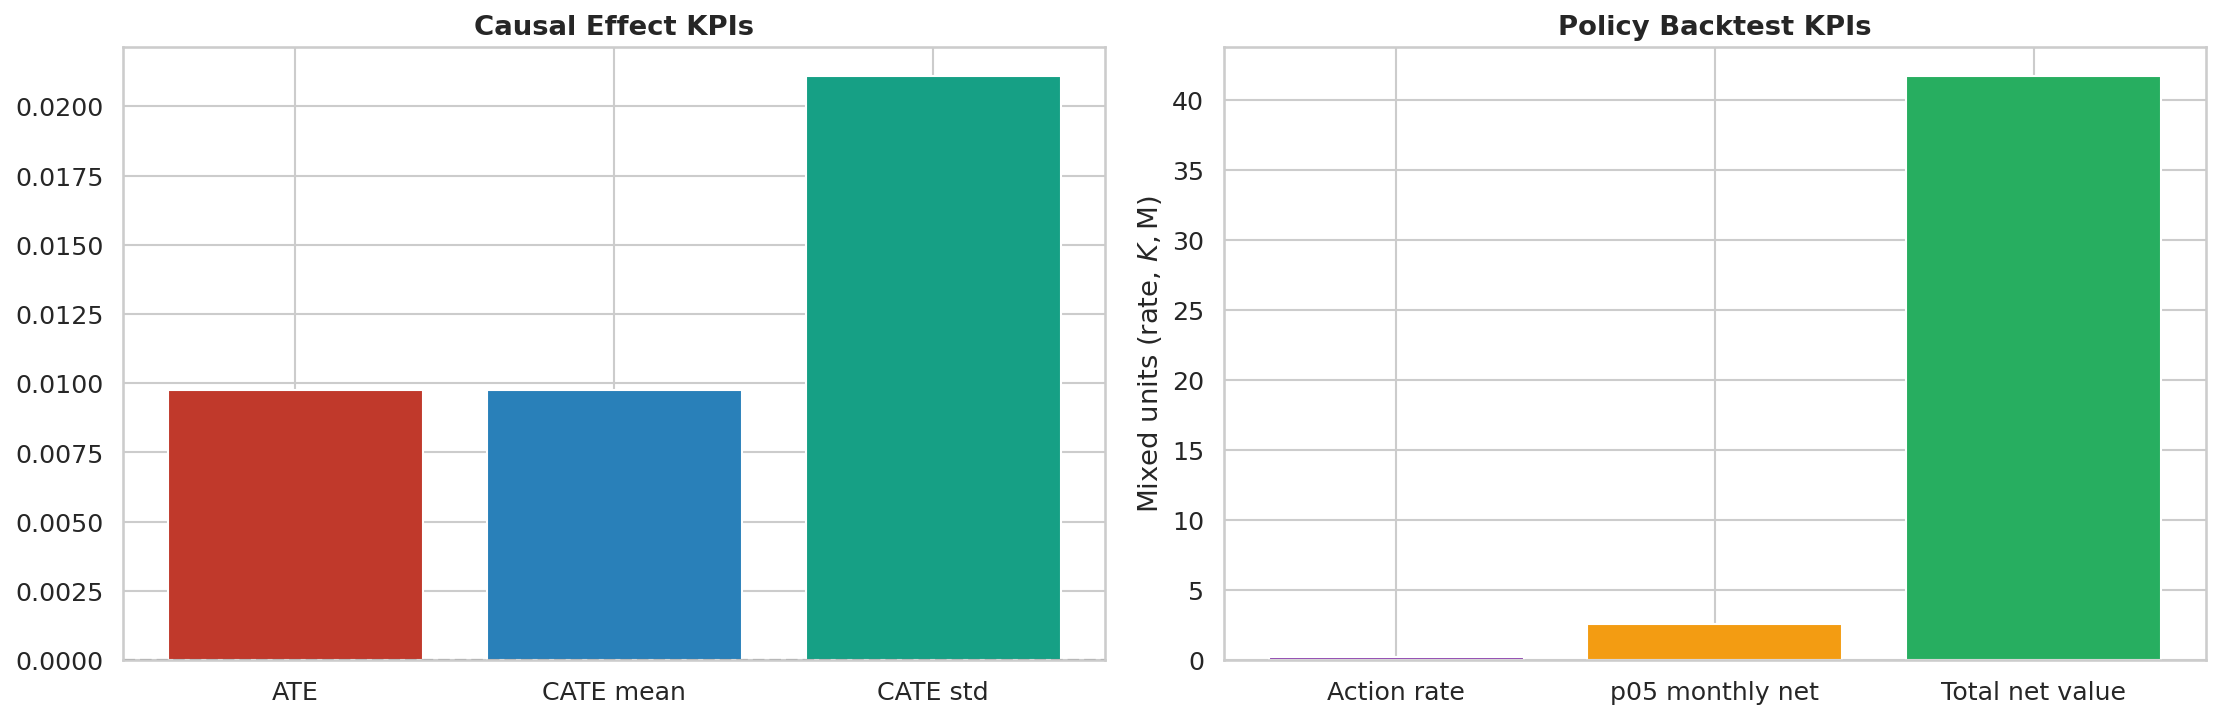
\includegraphics[keepaspectratio,alt={Indicadores clave de la política causal de pricing en el proyecto.}]{chapters/08-time-survival-causal/../../assets/figures/notebooks/causal_policy_kpis.png}}

}

\subcaption{KPIs de política causal y su efecto económico sobre
decisiones segmentadas de precio.}

\end{figure}%

\end{minipage}%

\end{figure*}%

\begin{table}

\caption{\label{tbl-temporal-causal-overview}Resumen de los bloques
temporales y causales del pipeline}

\centering{

\begin{Shaded}
\begin{Highlighting}[]
\ImportTok{import}\NormalTok{ pandas }\ImportTok{as}\NormalTok{ pd}

\NormalTok{overview }\OperatorTok{=}\NormalTok{ [}
\NormalTok{    \{}\StringTok{"Bloque"}\NormalTok{: }\StringTok{"Supervivencia"}\NormalTok{, }\StringTok{"Pregunta"}\NormalTok{: }\StringTok{"Cuándo ocurre el default"}\NormalTok{,}
     \StringTok{"Modelos"}\NormalTok{: }\StringTok{"Cox PH, RSF, CIF (Aalen{-}Johansen)"}\NormalTok{, }\StringTok{"Métrica clave"}\NormalTok{: }\StringTok{"C{-}index RSF = 0.6797"}\NormalTok{,}
     \StringTok{"Uso IFRS9"}\NormalTok{: }\StringTok{"PD lifetime (Stage 2)"}\NormalTok{\},}
\NormalTok{    \{}\StringTok{"Bloque"}\NormalTok{: }\StringTok{"Series de Tiempo"}\NormalTok{, }\StringTok{"Pregunta"}\NormalTok{: }\StringTok{"Hacia dónde va la tasa agregada"}\NormalTok{,}
     \StringTok{"Modelos"}\NormalTok{: }\StringTok{"AutoARIMA, AutoETS, StatsForecast"}\NormalTok{, }\StringTok{"Métrica clave"}\NormalTok{: }\StringTok{"temporal\_pd\_mult = 1.017"}\NormalTok{,}
     \StringTok{"Uso IFRS9"}\NormalTok{: }\StringTok{"Escenarios macro (baseline/adverse)"}\NormalTok{\},}
\NormalTok{    \{}\StringTok{"Bloque"}\NormalTok{: }\StringTok{"Inferencia Causal"}\NormalTok{, }\StringTok{"Pregunta"}\NormalTok{: }\StringTok{"Por qué (efecto causal de la tasa)"}\NormalTok{,}
     \StringTok{"Modelos"}\NormalTok{: }\StringTok{"DoWhy + CausalForestDML (EconML)"}\NormalTok{, }\StringTok{"Métrica clave"}\NormalTok{: }\StringTok{"ATE = +0.00974 pp"}\NormalTok{,}
     \StringTok{"Uso IFRS9"}\NormalTok{: }\StringTok{"Política de precio por segmento"}\NormalTok{\},}
\NormalTok{    \{}\StringTok{"Bloque"}\NormalTok{: }\StringTok{"Simulación A/B"}\NormalTok{, }\StringTok{"Pregunta"}\NormalTok{: }\StringTok{"Cuánto vale la robustez"}\NormalTok{,}
     \StringTok{"Modelos"}\NormalTok{: }\StringTok{"Bootstrap, permutación, t{-}test"}\NormalTok{, }\StringTok{"Métrica clave"}\NormalTok{: }\StringTok{"Significancia estadística"}\NormalTok{,}
     \StringTok{"Uso IFRS9"}\NormalTok{: }\StringTok{"Validación económica retrospectiva"}\NormalTok{\},}
\NormalTok{]}

\NormalTok{pd.DataFrame(overview)}
\end{Highlighting}
\end{Shaded}

}

\end{table}%

\begin{tcolorbox}[enhanced jigsaw, arc=.35mm, bottomrule=.15mm, bottomtitle=1mm, breakable, colback=white, colbacktitle=quarto-callout-note-color!10!white, colframe=quarto-callout-note-color-frame, coltitle=black, left=2mm, leftrule=.75mm, opacityback=0, opacitybacktitle=0.6, rightrule=.15mm, title=\textcolor{quarto-callout-note-color}{\faInfo}\hspace{0.5em}{Conexión con el pipeline principal}, titlerule=0mm, toprule=.15mm, toptitle=1mm]

Cada bloque consume artefactos del pipeline PD
(Capítulo~\ref{sec-catboost-tuned}) e intervalos conformal
(Capítulo~\ref{sec-split-conformal}), y produce insumos para provisiones
IFRS9 (Capítulo~\ref{sec-ecl-calculation}) o para la optimización de
portafolio (Capítulo~\ref{sec-robust-portfolio}). La cadena es:
\textbf{predicción cross-sectional} \(\rightarrow\) \textbf{dimensión
temporal} \(\rightarrow\) \textbf{decisión causal} \(\rightarrow\)
\textbf{validación A/B}.

\end{tcolorbox}

\chapter{Análisis de Supervivencia}\label{sec-survival}

\subsection{De la PD Puntual a la PD
Temporal}\label{de-la-pd-puntual-a-la-pd-temporal}

Un modelo de clasificación binaria asigna a cada préstamo una
probabilidad de incumplimiento (PD), pero no dice \emph{cuándo} podría
ocurrir ese incumplimiento. Dos préstamos con PD = 10\% tienen riesgo
nominal idéntico; sin embargo, si uno incumple en el mes 3 y otro en el
mes 48, la pérdida económica real es radicalmente diferente --- el
primero apenas ha amortizado capital, mientras que el segundo ya ha
devuelto la mayor parte del saldo.

El análisis de supervivencia modela explícitamente el \textbf{tiempo
hasta el evento} (time-to-default), generando curvas de probabilidad
acumulada a cualquier horizonte temporal. Esto es un insumo directo
para:

\begin{itemize}
\tightlist
\item
  \textbf{IFRS9 Stage 2}: Provisiones basadas en PD lifetime, no en PD a
  12 meses.
\item
  \textbf{Priorización de seguimiento}: Préstamos con riesgo de
  incumplimiento temprano requieren intervención inmediata.
\item
  \textbf{Valoración de cartera}: El timing del default afecta los
  flujos de caja descontados.
\end{itemize}

\subsection{Modelos Implementados}\label{modelos-implementados}

\subsubsection{Cox Proportional Hazards}\label{cox-proportional-hazards}

El modelo de Cox PH (Cox, 1972) es semi-paramétrico: estima la
\textbf{función de riesgo instantáneo} (hazard) como el producto de un
baseline hazard no especificado y un componente multiplicativo de
covariables:

\begin{equation}\protect\phantomsection\label{eq-cox-hazard}{
h(t \mid \mathbf{x}) = h_0(t) \exp(\boldsymbol{\beta}^T \mathbf{x})
}\end{equation}

donde \(h_0(t)\) es el baseline hazard y \(\boldsymbol{\beta}\) son los
coeficientes que se interpretan como log-hazard ratios. Un hazard ratio
\(\exp(\beta_j) > 1\) indica que un incremento unitario en \(x_j\)
aumenta proporcionalmente el riesgo de default en cualquier instante
\(t\).

La implementación utiliza \texttt{lifelines.CoxPHFitter} con
penalización L2 (\(\lambda = 0.01\)) para estabilidad numérica:

\begin{Shaded}
\begin{Highlighting}[]
\ImportTok{from}\NormalTok{ lifelines }\ImportTok{import}\NormalTok{ CoxPHFitter}

\NormalTok{cph }\OperatorTok{=}\NormalTok{ CoxPHFitter(penalizer}\OperatorTok{=}\FloatTok{0.01}\NormalTok{)}
\NormalTok{cph.fit(df[cols], duration\_col}\OperatorTok{=}\StringTok{"time\_to\_event"}\NormalTok{, event\_col}\OperatorTok{=}\StringTok{"event\_observed"}\NormalTok{)}
\end{Highlighting}
\end{Shaded}

\begin{tcolorbox}[enhanced jigsaw, arc=.35mm, bottomrule=.15mm, bottomtitle=1mm, breakable, colback=white, colbacktitle=quarto-callout-note-color!10!white, colframe=quarto-callout-note-color-frame, coltitle=black, left=2mm, leftrule=.75mm, opacityback=0, opacitybacktitle=0.6, rightrule=.15mm, title=\textcolor{quarto-callout-note-color}{\faInfo}\hspace{0.5em}{Supuesto de proporcionalidad}, titlerule=0mm, toprule=.15mm, toptitle=1mm]

El modelo Cox PH asume que los hazard ratios son constantes en el tiempo
--- la función \texttt{check\_assumptions()} valida este supuesto
mediante tests de Schoenfeld. Cuando se viola, el RSF es preferible
porque no impone restricciones sobre la forma de la relación
hazard-covariables.

\end{tcolorbox}

\subsubsection{Random Survival Forest
(RSF)}\label{random-survival-forest-rsf}

El Random Survival Forest (Ishwaran et~al., 2008) es un ensemble de
árboles de supervivencia que estima la función de supervivencia
\(S(t \mid \mathbf{x}) = P(T > t \mid \mathbf{x})\) de forma no
paramétrica. A diferencia de Cox PH, el RSF captura interacciones y
no-linealidades sin requerir el supuesto de proporcionalidad.

La configuración utilizada en el proyecto:

\begin{Shaded}
\begin{Highlighting}[]
\ImportTok{from}\NormalTok{ sksurv.ensemble }\ImportTok{import}\NormalTok{ RandomSurvivalForest}

\NormalTok{rsf }\OperatorTok{=}\NormalTok{ RandomSurvivalForest(}
\NormalTok{    n\_estimators}\OperatorTok{=}\DecValTok{500}\NormalTok{,}
\NormalTok{    min\_samples\_split}\OperatorTok{=}\DecValTok{10}\NormalTok{,}
\NormalTok{    min\_samples\_leaf}\OperatorTok{=}\DecValTok{5}\NormalTok{,}
\NormalTok{    max\_features}\OperatorTok{=}\StringTok{"sqrt"}\NormalTok{,}
\NormalTok{    random\_state}\OperatorTok{=}\DecValTok{42}\NormalTok{,}
\NormalTok{    n\_jobs}\OperatorTok{={-}}\DecValTok{1}\NormalTok{,}
\NormalTok{)}
\end{Highlighting}
\end{Shaded}

La métrica de evaluación es el \textbf{C-index} (concordancia de
Harrell): la probabilidad de que, dados dos préstamos, el modelo ordene
correctamente cuál incumple primero. Un C-index de 0.5 es aleatorio; 1.0
es perfecto. El RSF alcanza un \textbf{C-index = 0.6797} en el conjunto
OOT, indicando capacidad discriminativa moderada --- consistente con la
dificultad inherente de predecir el timing exacto de default en crédito
al consumo.

\subsection{Riesgos Competitivos y la Función de Incidencia
Acumulada}\label{riesgos-competitivos-y-la-funciuxf3n-de-incidencia-acumulada}

Un préstamo no solo puede hacer default: también puede \textbf{prepagar}
antes de su vencimiento. Estos dos eventos compiten entre sí, y
tratarlos correctamente requiere un marco de \textbf{riesgos
competitivos} (competing risks).

El estimador estándar de Kaplan-Meier ignora los riesgos competitivos:
trata los prepagos como censura, lo que \textbf{sobreestima} la
probabilidad acumulada de default. El estimador de
\textbf{Aalen-Johansen} calcula la \textbf{Cumulative Incidence
Function} (CIF) correcta, separando las probabilidades acumuladas de
default y prepago:

\begin{equation}\protect\phantomsection\label{eq-cif}{
\text{CIF}_k(t) = \int_0^t S(u^{-}) \, dH_k(u)
}\end{equation}

donde \(S(u^{-})\) es la supervivencia global justo antes de \(u\) y
\(H_k\) es el hazard acumulado causa-específico para el evento \(k\).

\begin{tcolorbox}[enhanced jigsaw, arc=.35mm, bottomrule=.15mm, bottomtitle=1mm, breakable, colback=white, colbacktitle=quarto-callout-warning-color!10!white, colframe=quarto-callout-warning-color-frame, coltitle=black, left=2mm, leftrule=.75mm, opacityback=0, opacitybacktitle=0.6, rightrule=.15mm, title=\textcolor{quarto-callout-warning-color}{\faExclamationTriangle}\hspace{0.5em}{KM vs CIF: Sobreestimación del 26.7\%}, titlerule=0mm, toprule=.15mm, toptitle=1mm]

En el dataset, Kaplan-Meier sobreestima la PD lifetime en
\textbf{26.7\%} respecto a la CIF correcta. Esto se traduce en un exceso
de reserva de \textbf{\$125.8M} (12.6\% de la provisión ECL calculada
con KM). Para provisiones IFRS9, la CIF debe usarse siempre que existan
eventos competitivos --- lo cual es la norma en carteras de crédito al
consumo.

\end{tcolorbox}

La implementación en \texttt{src/models/survival.py} utiliza
\texttt{sksurv.nonparametric.cumulative\_incidence\_competing\_risks}
con estratificación por grado:

\begin{Shaded}
\begin{Highlighting}[]
\ImportTok{from}\NormalTok{ sksurv.nonparametric }\ImportTok{import}\NormalTok{ cumulative\_incidence\_competing\_risks}

\CommentTok{\# status\_encoded: 0=censored, 1=default, 2=prepayment}
\NormalTok{result }\OperatorTok{=}\NormalTok{ cumulative\_incidence\_competing\_risks(}
\NormalTok{    status\_encoded, time, conf\_level}\OperatorTok{=}\FloatTok{0.95}\NormalTok{, conf\_type}\OperatorTok{=}\StringTok{"log{-}log"}
\NormalTok{)}
\end{Highlighting}
\end{Shaded}

\begin{figure*}

\centering{

\pandocbounded{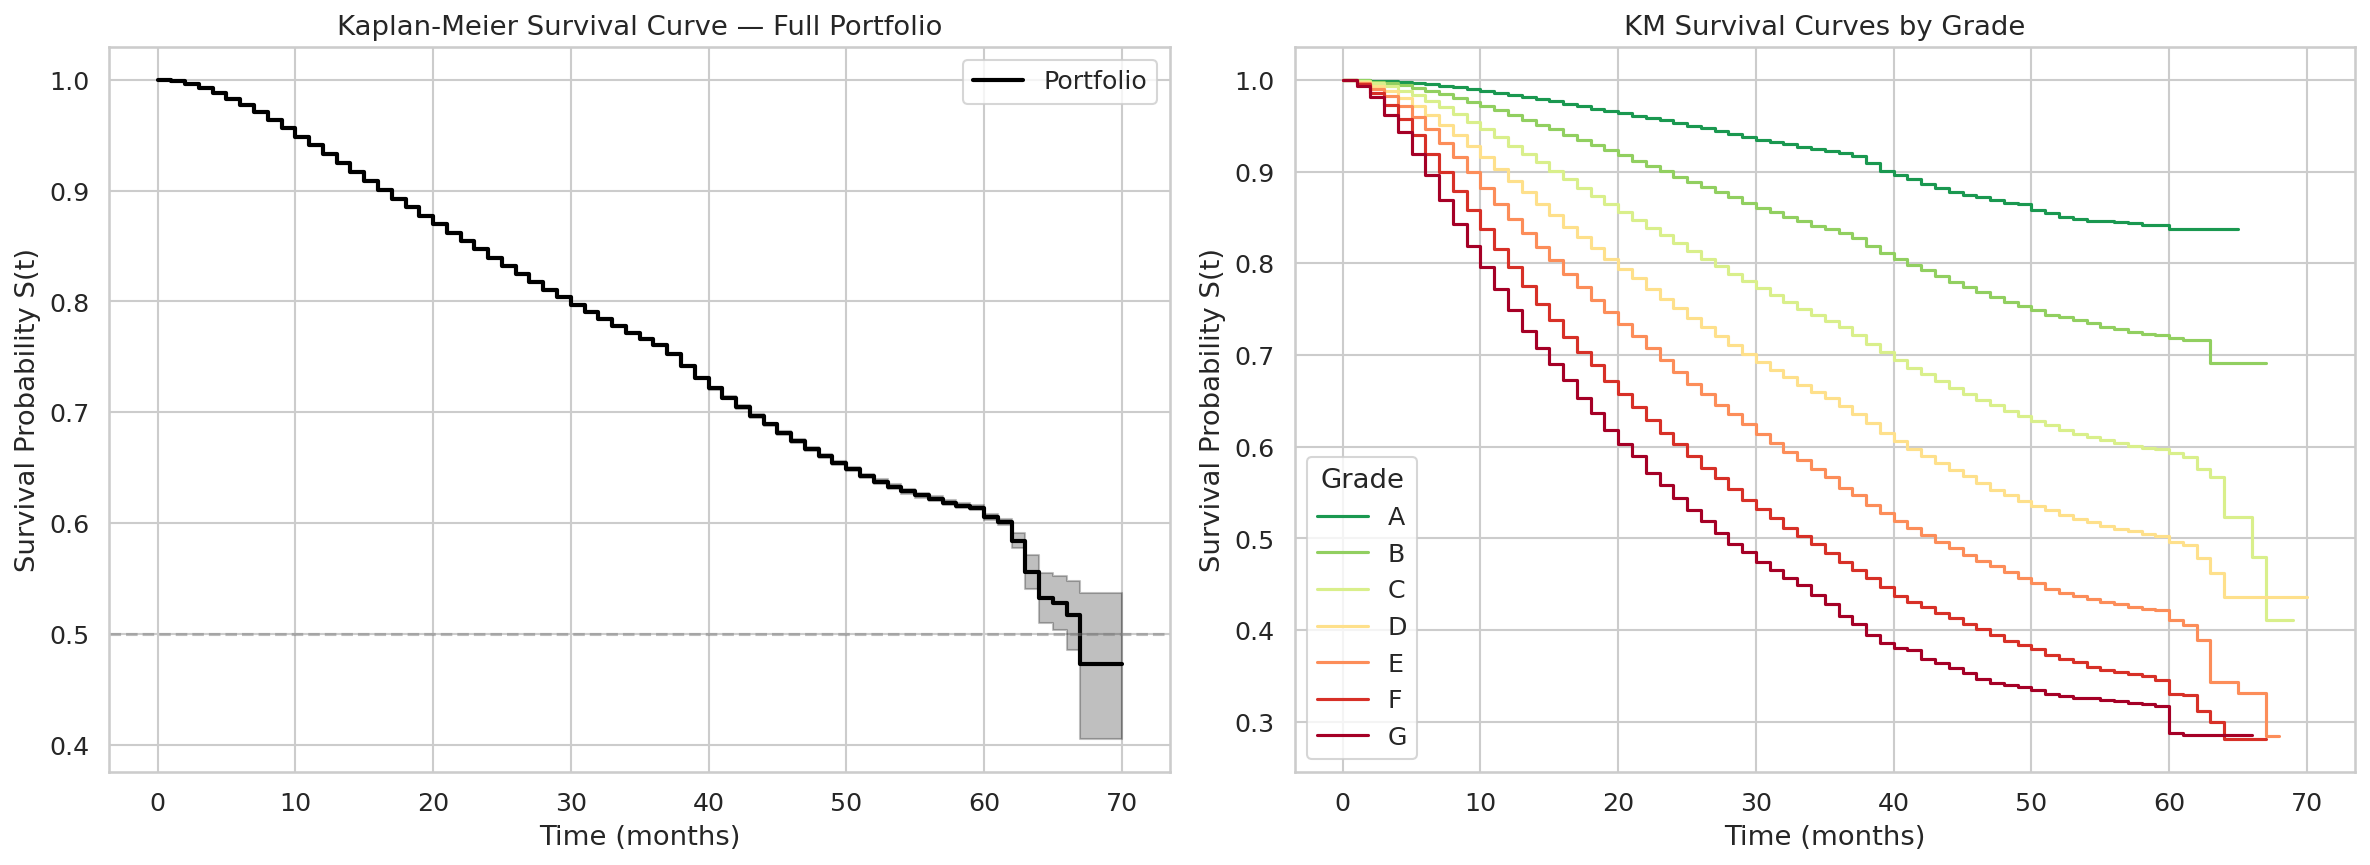
\includegraphics[keepaspectratio,alt={Curvas Kaplan-Meier y funciones de supervivencia para segmentos del dataset Lending Club.}]{chapters/08-time-survival-causal/../../assets/figures/notebooks/kaplan_meier_curves.png}}

}

\caption{\label{fig-kaplan-meier}Curvas de supervivencia y default
acumulado por segmento, generadas desde los notebooks del bloque
temporal y de supervivencia.}

\end{figure*}%

La figura Figura~\ref{fig-kaplan-meier} aterriza la intuición temporal:
no basta con saber quién es riesgoso; importa cuándo emerge ese riesgo y
cómo difiere entre segmentos.

\subsection{Curvas de PD Lifetime para
IFRS9}\label{curvas-de-pd-lifetime-para-ifrs9}

La función \texttt{generate\_lifetime\_pd\_curve()} genera
probabilidades acumuladas de default a intervalos de 30 días hasta 5
años (60 meses), que son el insumo directo para el cálculo de ECL
lifetime en IFRS9 Stage 2:

\[
\text{PD}_{\text{lifetime}}(t) = 1 - S(t \mid \mathbf{x})
\]

\begin{table}

\caption{\label{tbl-survival-summary}Resumen de modelos de supervivencia
y métricas clave}

\centering{

\begin{Shaded}
\begin{Highlighting}[]
\ImportTok{import}\NormalTok{ sys}
\ImportTok{from}\NormalTok{ pathlib }\ImportTok{import}\NormalTok{ Path}

\NormalTok{sys.path.insert(}\DecValTok{0}\NormalTok{, }\BuiltInTok{str}\NormalTok{(Path.cwd().parent }\ControlFlowTok{if}\NormalTok{ Path.cwd().name }\OperatorTok{==} \StringTok{"book"} \ControlFlowTok{else}\NormalTok{ Path.cwd()))}
\ImportTok{from}\NormalTok{ book.\_helpers.load\_artifacts }\ImportTok{import}\NormalTok{ try\_load\_json}

\ImportTok{import}\NormalTok{ pandas }\ImportTok{as}\NormalTok{ pd}

\NormalTok{summary }\OperatorTok{=}\NormalTok{ try\_load\_json(}\StringTok{"pipeline\_summary"}\NormalTok{)}
\NormalTok{surv }\OperatorTok{=}\NormalTok{ summary.get(}\StringTok{"survival"}\NormalTok{, \{\})}

\NormalTok{rows }\OperatorTok{=}\NormalTok{ [}
\NormalTok{    \{}\StringTok{"Modelo"}\NormalTok{: }\StringTok{"Cox PH"}\NormalTok{, }\StringTok{"Tipo"}\NormalTok{: }\StringTok{"Semi{-}paramétrico"}\NormalTok{,}
     \StringTok{"C{-}index"}\NormalTok{: }\SpecialStringTok{f"}\SpecialCharTok{\{}\NormalTok{surv}\SpecialCharTok{.}\NormalTok{get(}\StringTok{\textquotesingle{}cox\_concordance\textquotesingle{}}\NormalTok{, }\DecValTok{0}\NormalTok{)}\SpecialCharTok{:.4f\}}\SpecialStringTok{"}\NormalTok{,}
     \StringTok{"Ventaja"}\NormalTok{: }\StringTok{"Interpretable (hazard ratios)"}\NormalTok{, }\StringTok{"Limitación"}\NormalTok{: }\StringTok{"Supuesto de proporcionalidad"}\NormalTok{\},}
\NormalTok{    \{}\StringTok{"Modelo"}\NormalTok{: }\StringTok{"RSF (500 árboles)"}\NormalTok{, }\StringTok{"Tipo"}\NormalTok{: }\StringTok{"Ensemble no paramétrico"}\NormalTok{,}
     \StringTok{"C{-}index"}\NormalTok{: }\SpecialStringTok{f"}\SpecialCharTok{\{}\NormalTok{surv}\SpecialCharTok{.}\NormalTok{get(}\StringTok{\textquotesingle{}rsf\_concordance\textquotesingle{}}\NormalTok{, }\DecValTok{0}\NormalTok{)}\SpecialCharTok{:.4f\}}\SpecialStringTok{"}\NormalTok{,}
     \StringTok{"Ventaja"}\NormalTok{: }\StringTok{"Captura no{-}linealidades"}\NormalTok{, }\StringTok{"Limitación"}\NormalTok{: }\StringTok{"Menos interpretable"}\NormalTok{\},}
\NormalTok{    \{}\StringTok{"Modelo"}\NormalTok{: }\StringTok{"CIF (Aalen{-}Johansen)"}\NormalTok{, }\StringTok{"Tipo"}\NormalTok{: }\StringTok{"No paramétrico"}\NormalTok{,}
     \StringTok{"C{-}index"}\NormalTok{: }\StringTok{"{-}{-}{-}"}\NormalTok{,}
     \StringTok{"Ventaja"}\NormalTok{: }\StringTok{"Riesgos competitivos correctos"}\NormalTok{, }\StringTok{"Limitación"}\NormalTok{: }\StringTok{"No condicional a covariables"}\NormalTok{\},}
\NormalTok{]}

\NormalTok{pd.DataFrame(rows)}
\end{Highlighting}
\end{Shaded}

}

\end{table}%

\begin{tcolorbox}[enhanced jigsaw, arc=.35mm, bottomrule=.15mm, bottomtitle=1mm, breakable, colback=white, colbacktitle=quarto-callout-tip-color!10!white, colframe=quarto-callout-tip-color-frame, coltitle=black, left=2mm, leftrule=.75mm, opacityback=0, opacitybacktitle=0.6, rightrule=.15mm, title=\textcolor{quarto-callout-tip-color}{\faLightbulb}\hspace{0.5em}{Conexión con el pipeline}, titlerule=0mm, toprule=.15mm, toptitle=1mm]

Las curvas de PD lifetime alimentan directamente el cálculo de ECL en
Capítulo~\ref{sec-ecl-calculation}. La corrección CIF \(\rightarrow\) KM
evita sobreprovisionar por \$125.8M. Los hazard ratios de Cox PH
complementan la interpretación de los coeficientes SHAP del modelo PD
(Capítulo~\ref{sec-global-explanations}), proporcionando una perspectiva
temporal sobre los mismos drivers de riesgo.

\end{tcolorbox}

\chapter{Pronóstico de Series de Tiempo}\label{sec-time-series}

\subsection{Motivación: El Default Agregado como Señal
Macro}\label{motivaciuxf3n-el-default-agregado-como-seuxf1al-macro}

Mientras que la PD modela el riesgo individual de cada préstamo, la
\textbf{tasa de default agregada mensual} captura dinámicas de nivel
portafolio que no son visibles desde la predicción cross-sectional:
estacionalidad, tendencias macroeconómicas y cambios de régimen. Estas
señales temporales son el insumo para:

\begin{itemize}
\tightlist
\item
  \textbf{Escenarios IFRS9}: Los multiplicadores
  \texttt{temporal\_pd\_baseline\_mult} ajustan la PD puntual según el
  régimen temporal proyectado.
\item
  \textbf{Planeación de provisiones}: Anticipar deterioro antes de que
  se materialice en defaults realizados.
\item
  \textbf{Apetito de riesgo}: Ajustar políticas de originación según la
  tendencia proyectada.
\end{itemize}

El dataset de series de tiempo (\texttt{time\_series.parquet}) contiene
118 observaciones mensuales agregadas con formato Nixtla-ready
(\texttt{unique\_id}, \texttt{ds}, \texttt{y}), donde \texttt{y} es la
tasa de default mensual del portafolio.

\subsection{Framework de Pronóstico
Gobernado}\label{framework-de-pronuxf3stico-gobernado}

El módulo \texttt{src/models/time\_series.py} implementa un framework
completo de pronóstico con selección automática de champion, backtest
por rolling-origin y gobernanza de estado (oficial vs.~exploratorio):

\begin{figure*}

\begin{figure}[H]

{\centering \pandocbounded{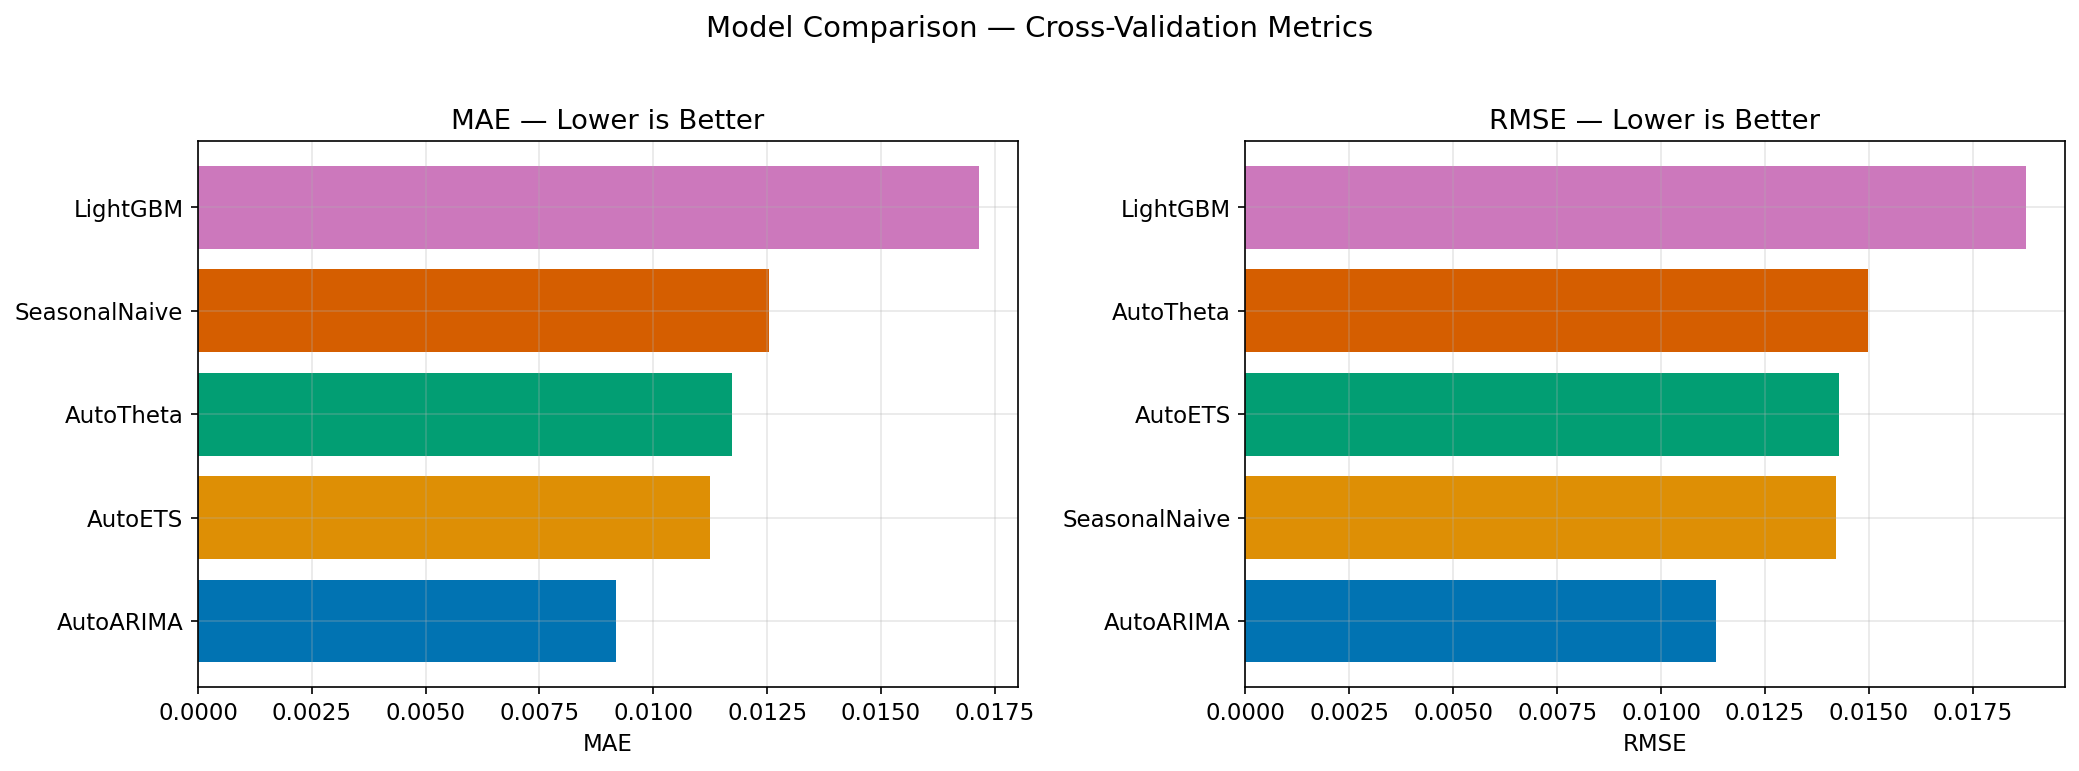
\includegraphics[keepaspectratio,alt={Comparación de modelos de forecasting en validación temporal.}]{chapters/08-time-survival-causal/../../assets/figures/notebooks/cv_model_comparison.png}}

}

\caption{Comparación de modelos en validación cruzada rolling-origin
para series de tiempo.}

\end{figure}%

\end{figure*}%

\subsubsection{Modelos Candidatos}\label{modelos-candidatos}

La librería StatsForecast provee los modelos estadísticos base, todos
evaluados en backtest:

{\def\LTcaptype{none} % do not increment counter
\begin{longtable}[]{@{}
  >{\raggedright\arraybackslash}p{(\linewidth - 4\tabcolsep) * \real{0.2667}}
  >{\raggedright\arraybackslash}p{(\linewidth - 4\tabcolsep) * \real{0.3000}}
  >{\raggedright\arraybackslash}p{(\linewidth - 4\tabcolsep) * \real{0.4333}}@{}}
\toprule\noalign{}
\begin{minipage}[b]{\linewidth}\raggedright
Modelo
\end{minipage} & \begin{minipage}[b]{\linewidth}\raggedright
Familia
\end{minipage} & \begin{minipage}[b]{\linewidth}\raggedright
Descripción
\end{minipage} \\
\midrule\noalign{}
\endhead
\bottomrule\noalign{}
\endlastfoot
SeasonalNaive & Benchmark & Repite el valor de hace 12 meses \\
AutoARIMA & Estadístico & Selección automática de orden
(p,d,q)(P,D,Q) \\
AutoETS & Estadístico & Error-Trend-Seasonality con selección por AIC \\
AutoTheta & Estadístico & Método Theta con descomposición \\
SARIMAX & Challenger & ARIMA estacional con covariables exógenas \\
STL\_CatBoost & ML & Descomposición STL + residuos con CatBoost \\
\end{longtable}
}

La selección de champion sigue una política declarativa configurada en
\texttt{configs/time\_series.yaml}: la métrica primaria es \textbf{MASE}
(Mean Absolute Scaled Error), con desempates por RMSSE y sesgo absoluto.
El champion debe superar al SeasonalNaive para ser promovido a estado
oficial.

\subsubsection{Backtest por
Rolling-Origin}\label{backtest-por-rolling-origin}

A diferencia del train/test split único, el backtest utiliza
\textbf{rolling-origin} con ventanas expandibles:

\begin{itemize}
\tightlist
\item
  \textbf{Entrenamiento mínimo}: 72 periodos (6 años).
\item
  \textbf{Horizonte}: 12 meses adelante.
\item
  \textbf{Paso}: 1 mes entre cutoffs sucesivos.
\item
  \textbf{Máximo de ventanas}: 36 (3 años de evaluación).
\end{itemize}

Esta estrategia evalúa la estabilidad del pronóstico a lo largo de
distintos regímenes temporales, no solo sobre un corte fijo.

\subsection{Estado del Pronóstico: Oficial
vs.~Exploratorio}\label{estado-del-pronuxf3stico-oficial-vs.-exploratorio}

\begin{tcolorbox}[enhanced jigsaw, arc=.35mm, bottomrule=.15mm, bottomtitle=1mm, breakable, colback=white, colbacktitle=quarto-callout-warning-color!10!white, colframe=quarto-callout-warning-color-frame, coltitle=black, left=2mm, leftrule=.75mm, opacityback=0, opacitybacktitle=0.6, rightrule=.15mm, title=\textcolor{quarto-callout-warning-color}{\faExclamationTriangle}\hspace{0.5em}{Status: research\_only}, titlerule=0mm, toprule=.15mm, toptitle=1mm]

El bloque de series de tiempo tiene status \texttt{research\_only} en el
pipeline actual. Esto significa que los pronósticos se generan y
evalúan, pero no se promueven automáticamente a insumos oficiales para
IFRS9 o decisiones de portafolio. La promoción requiere evidencia
suficiente de backtest (cobertura y calibración) según la política de
gobernanza.

\end{tcolorbox}

El framework distingue tres niveles de estado:

\begin{enumerate}
\def\labelenumi{\arabic{enumi}.}
\tightlist
\item
  \textbf{official}: Backtest satisfactorio, cobertura de intervalos
  dentro de tolerancia, champion supera benchmark. El pronóstico puede
  usarse como insumo de provisiones.
\item
  \textbf{warn}: Métricas cercanas al umbral. Se genera el pronóstico
  pero con alertas de gobernanza.
\item
  \textbf{research\_only}: Evidencia insuficiente. El pronóstico es
  informativo pero no se usa en decisiones automatizadas.
\end{enumerate}

\subsection{Escenarios IFRS9 y Multiplicador
Temporal}\label{escenarios-ifrs9-y-multiplicador-temporal}

El pronóstico genera tres escenarios para el cálculo de ECL:

\begin{equation}\protect\phantomsection\label{eq-temporal-mult}{
\text{PD}_{\text{ajustada}} = \text{PD}_{\text{puntual}} \times \text{temporal\_pd\_baseline\_mult}
}\end{equation}

donde \texttt{temporal\_pd\_baseline\_mult} es el ratio entre la PD
promedio proyectada y la PD promedio histórica. En el run champion, este
multiplicador es \textbf{1.017154}, indicando un deterioro marginal
proyectado del 1.7\% respecto al baseline histórico.

\begin{table}

\caption{\label{tbl-ts-scenarios}Escenarios temporales para ajuste de PD
en IFRS9}

\centering{

\begin{Shaded}
\begin{Highlighting}[]
\ImportTok{import}\NormalTok{ pandas }\ImportTok{as}\NormalTok{ pd}

\NormalTok{scenarios }\OperatorTok{=}\NormalTok{ [}
\NormalTok{    \{}\StringTok{"Escenario"}\NormalTok{: }\StringTok{"Optimista (P10)"}\NormalTok{, }\StringTok{"Descripción"}\NormalTok{: }\StringTok{"Banda inferior del intervalo de pronóstico"}\NormalTok{,}
     \StringTok{"Uso"}\NormalTok{: }\StringTok{"Piso de provisiones"}\NormalTok{, }\StringTok{"Fuente"}\NormalTok{: }\StringTok{"y\_lo\_90 del forecast"}\NormalTok{\},}
\NormalTok{    \{}\StringTok{"Escenario"}\NormalTok{: }\StringTok{"Baseline"}\NormalTok{, }\StringTok{"Descripción"}\NormalTok{: }\StringTok{"Pronóstico puntual del champion"}\NormalTok{,}
     \StringTok{"Uso"}\NormalTok{: }\StringTok{"Provisión central (temporal\_pd\_mult = 1.017)"}\NormalTok{,}
     \StringTok{"Fuente"}\NormalTok{: }\StringTok{"y del forecast"}\NormalTok{\},}
\NormalTok{    \{}\StringTok{"Escenario"}\NormalTok{: }\StringTok{"Adverso (P90)"}\NormalTok{, }\StringTok{"Descripción"}\NormalTok{: }\StringTok{"Banda superior del intervalo de pronóstico"}\NormalTok{,}
     \StringTok{"Uso"}\NormalTok{: }\StringTok{"Techo de provisiones / stress test"}\NormalTok{,}
     \StringTok{"Fuente"}\NormalTok{: }\StringTok{"y\_hi\_90 del forecast"}\NormalTok{\},}
\NormalTok{]}

\NormalTok{pd.DataFrame(scenarios)}
\end{Highlighting}
\end{Shaded}

}

\end{table}%

\begin{figure*}

\centering{

\pandocbounded{\includegraphics[keepaspectratio,alt={Fan chart del pronóstico de tasas de default para IFRS9 con bandas de incertidumbre.}]{chapters/08-time-survival-causal/../../assets/figures/notebooks/ifrs9_scenario_fan_chart.png}}

}

\caption{\label{fig-ifrs9-fan-chart}Fan chart del forecast IFRS9 con
bandas de incertidumbre y escenarios baseline, optimista y adverso.}

\end{figure*}%

La figura Figura~\ref{fig-ifrs9-fan-chart} deja visible la propagación
de incertidumbre temporal: un abanico relativamente moderado en la tasa
agregada se amplifica al pasar por LGD y EAD.

\subsection{Propagación de Intervalos a
ECL}\label{propagaciuxf3n-de-intervalos-a-ecl}

Los intervalos de pronóstico temporal se propagan de forma no lineal al
cálculo de ECL. En el análisis de Paper 2, la banda de ECL resultante es
de \textbf{\$288.5M} (267\% del ECL puntual de \$107.9M), con un
escenario adverso de \$336M versus un optimista de \$47.5M. Esta
amplificación refleja que la incertidumbre en forecasts cercanos a cero
se propaga de forma no lineal cuando se multiplica por LGD y EAD.

\begin{tcolorbox}[enhanced jigsaw, arc=.35mm, bottomrule=.15mm, bottomtitle=1mm, breakable, colback=white, colbacktitle=quarto-callout-tip-color!10!white, colframe=quarto-callout-tip-color-frame, coltitle=black, left=2mm, leftrule=.75mm, opacityback=0, opacitybacktitle=0.6, rightrule=.15mm, title=\textcolor{quarto-callout-tip-color}{\faLightbulb}\hspace{0.5em}{Conexión con el pipeline}, titlerule=0mm, toprule=.15mm, toptitle=1mm]

El multiplicador temporal alimenta el cálculo de ECL en
Capítulo~\ref{sec-ecl-calculation}. Los escenarios adverso/optimista
definen la banda de provisiones bajo distintas hipótesis macro. La
reconciliación jerárquica (cuando está habilitada) garantiza
consistencia entre pronósticos a nivel portafolio y por grado/plazo.

\end{tcolorbox}

\chapter{Inferencia Causal}\label{sec-causal-inference}

\subsection{De Correlación a Causalidad en Riesgo de
Crédito}\label{de-correlaciuxf3n-a-causalidad-en-riesgo-de-cruxe9dito}

En el dataset de Lending Club, los préstamos con tasas de interés altas
tienen más defaults. Pero, la tasa alta \emph{causa} más defaults? O
simplemente se cobra más a quienes ya eran riesgosos? Responder esta
pregunta requiere pasar de asociación estadística a \textbf{estimación
causal}, distinguiendo la relación correlacional (útil para predicción)
de la relación causal (necesaria para intervención).

Esta distinción es operativamente crítica:

\begin{itemize}
\tightlist
\item
  \textbf{Correlación}: ``Los préstamos con tasa \textgreater20\% tienen
  24\% de default'' --- describe el pasado, útil para scoring.
\item
  \textbf{Causalidad}: ``Si movemos la tasa 1pp, el default esperado
  cambia en +0.00974pp'' --- permite diseñar políticas de precio.
\end{itemize}

El pipeline causal combina \textbf{DoWhy} para identificación y
refutación con \textbf{EconML} para estimación heterogénea, siguiendo el
marco de Double Machine Learning ({Chernozhukov et~al.}, 2018).

\subsection{Grafo Causal y Estrategia de
Identificación}\label{grafo-causal-y-estrategia-de-identificaciuxf3n}

La identificación del efecto causal requiere especificar un \textbf{DAG}
(Directed Acyclic Graph) con las relaciones causales asumidas. El grafo
oficial del proyecto establece:

\begin{figure*}

\begin{minipage}[t]{0.50\linewidth}

\begin{figure}[H]

{\centering \pandocbounded{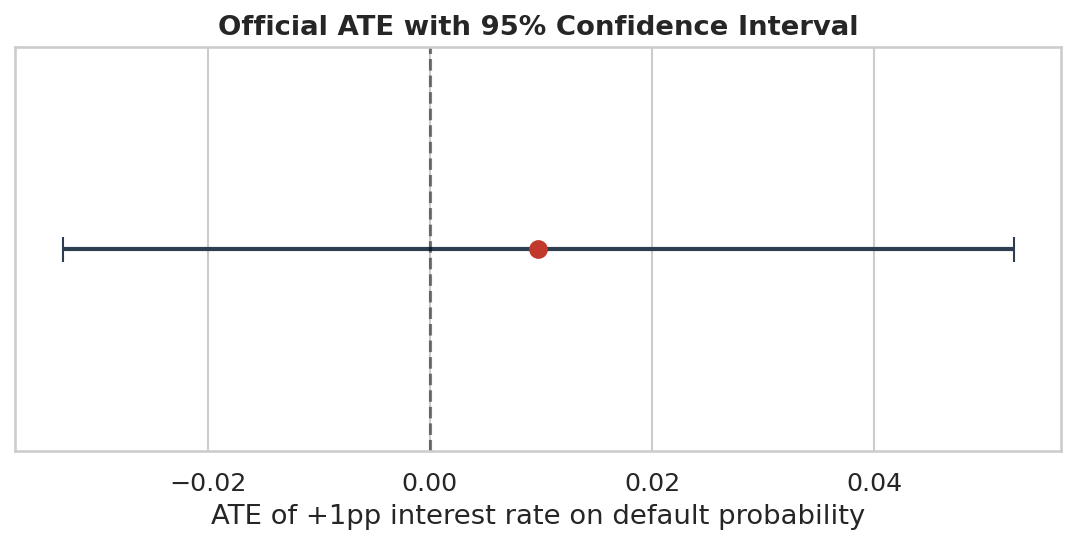
\includegraphics[keepaspectratio,alt={Intervalo de confianza del efecto promedio de tratamiento de la tasa de interés.}]{chapters/08-time-survival-causal/../../assets/figures/notebooks/ate_confidence_interval.png}}

}

\subcaption{Intervalo de confianza del ATE para la tasa de interés como
tratamiento.}

\end{figure}%

\end{minipage}%
%
\begin{minipage}[t]{0.50\linewidth}

\begin{figure}[H]

{\centering \pandocbounded{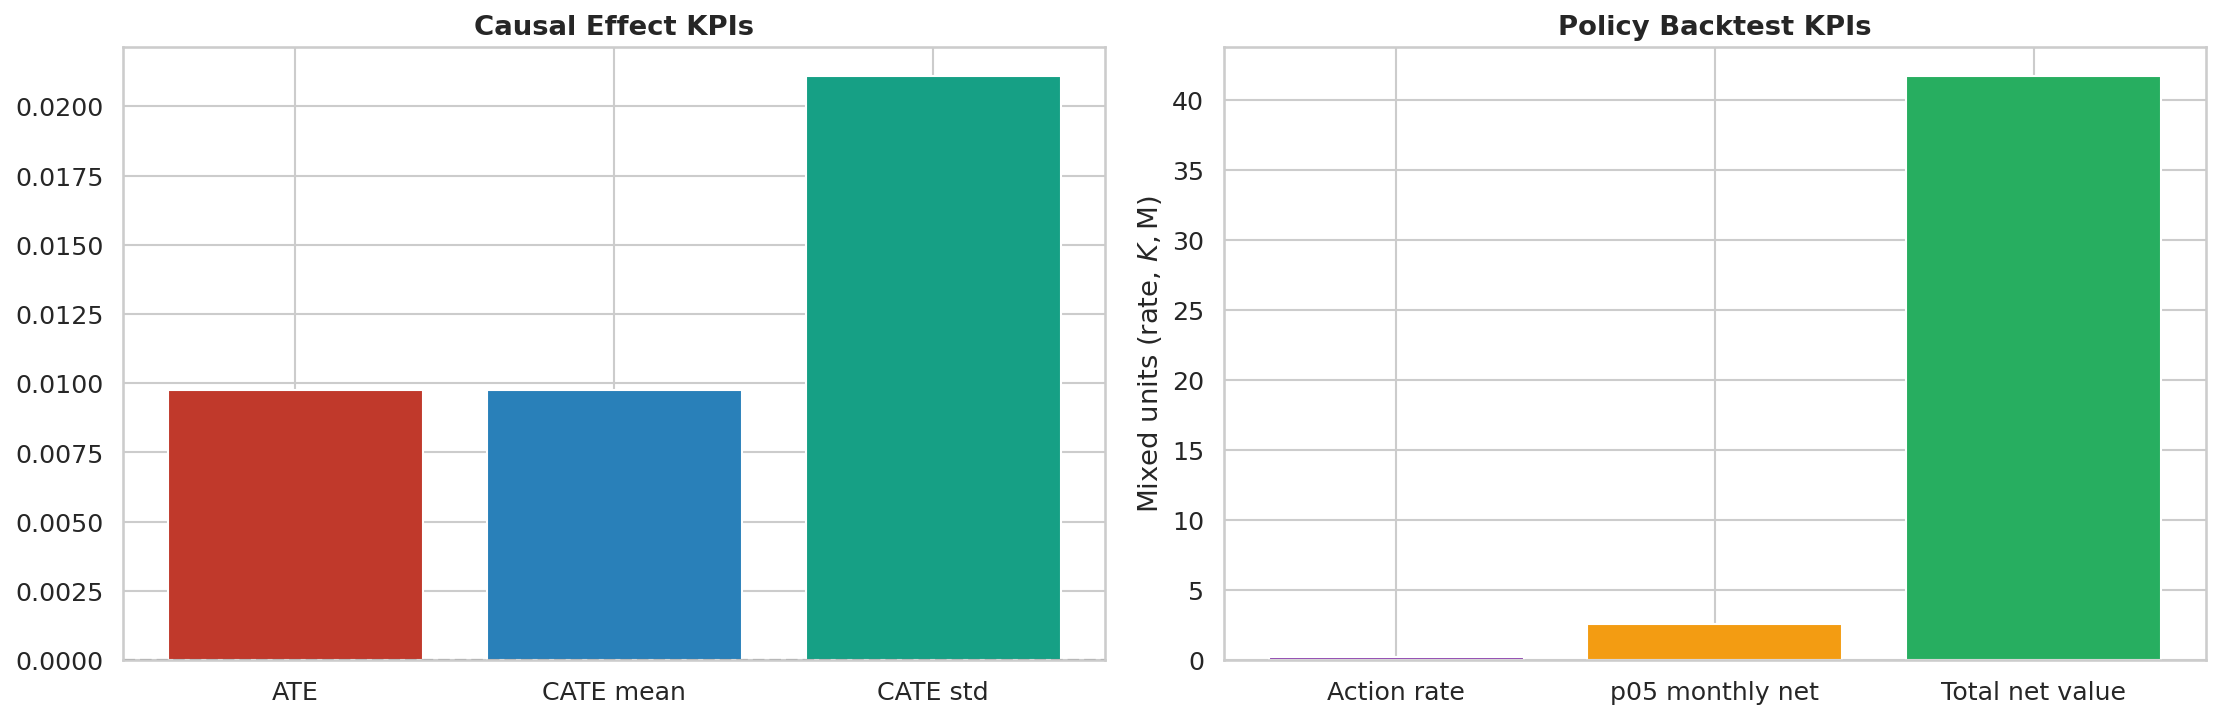
\includegraphics[keepaspectratio,alt={Indicadores de desempeño de la política causal aplicada al portafolio.}]{chapters/08-time-survival-causal/../../assets/figures/notebooks/causal_policy_kpis.png}}

}

\subcaption{KPIs operativos de la política causal simulada sobre el set
OOT.}

\end{figure}%

\end{minipage}%

\end{figure*}%

La estrategia de identificación es \textbf{backdoor adjustment}:
condicionando sobre los confusores (grade\_woe, purpose\_woe,
home\_ownership\_woe), la asignación de tratamiento (tasa de interés) se
vuelve \emph{as-if} aleatoria, permitiendo estimar el efecto causal.

\begin{tcolorbox}[enhanced jigsaw, arc=.35mm, bottomrule=.15mm, bottomtitle=1mm, breakable, colback=white, colbacktitle=quarto-callout-note-color!10!white, colframe=quarto-callout-note-color-frame, coltitle=black, left=2mm, leftrule=.75mm, opacityback=0, opacitybacktitle=0.6, rightrule=.15mm, title=\textcolor{quarto-callout-note-color}{\faInfo}\hspace{0.5em}{Supuestos de identificación}, titlerule=0mm, toprule=.15mm, toptitle=1mm]

La estimación causal observacional requiere tres supuestos clave:

\begin{enumerate}
\def\labelenumi{\arabic{enumi}.}
\tightlist
\item
  \textbf{Ignorabilidad condicional}: No hay confusores no observados
  que afecten simultáneamente tasa y default.
\item
  \textbf{Overlap (positividad)}: Para cada combinación de confusores,
  existen observaciones con diferentes niveles de tasa.
\item
  \textbf{Consistencia temporal}: Las covariables estaban disponibles al
  momento de la originación.
\end{enumerate}

Estos supuestos son no testables directamente, pero las
\textbf{refutaciones de DoWhy} proporcionan evidencia indirecta de su
plausibilidad.

\end{tcolorbox}

\subsection{Double Machine Learning
(DML)}\label{double-machine-learning-dml}

El framework DML ({Chernozhukov et~al.}, 2018) estima el efecto causal
en dos etapas, usando modelos de machine learning flexibles para
controlar confusores sin imponer formas funcionales:

\textbf{Etapa 1 --- Nuisance estimation:}
\begin{equation}\protect\phantomsection\label{eq-dml-residuals}{
\hat{Y}_{\text{res}} = Y - \hat{g}(W), \quad \hat{T}_{\text{res}} = T - \hat{m}(W)
}\end{equation}

donde \(\hat{g}\) y \(\hat{m}\) son GBM (Gradient Boosting Machines) que
predicen outcome y tratamiento a partir de confusores \(W\).

\textbf{Etapa 2 --- Estimación del efecto:}
\begin{equation}\protect\phantomsection\label{eq-dml-estimate}{
\hat{Y}_{\text{res}} = \theta \cdot \hat{T}_{\text{res}} + \epsilon
}\end{equation}

El estimador \(\hat{\theta}\) es el \textbf{Average Treatment Effect}
(ATE): el cambio promedio en la probabilidad de default por cada unidad
de cambio en la tasa de interés.

\subsection{Efecto Promedio (ATE)}\label{efecto-promedio-ate}

El ATE estimado por DoWhy con identificación backdoor y estimación por
regresión lineal es:

\[
\text{ATE} = +0.00974
\]

\textbf{Interpretación}: Un aumento de 1 punto porcentual en la tasa de
interés se asocia causalmente con un incremento de \textbf{0.974 puntos
porcentuales} en la probabilidad de default, controlando por grado,
propósito, vivienda, DTI, ingreso, monto y FICO.

\subsection{Efectos Heterogéneos (CATE) con
CausalForestDML}\label{efectos-heteroguxe9neos-cate-con-causalforestdml}

El ATE es un promedio global, pero el efecto de la tasa puede variar
sustancialmente entre segmentos. El \textbf{Conditional Average
Treatment Effect} (CATE) captura esta heterogeneidad usando
CausalForestDML (Athey \& Wager, 2019):

\begin{Shaded}
\begin{Highlighting}[]
\ImportTok{from}\NormalTok{ econml.dml }\ImportTok{import}\NormalTok{ CausalForestDML}

\NormalTok{est }\OperatorTok{=}\NormalTok{ CausalForestDML(}
\NormalTok{    model\_y}\OperatorTok{=}\NormalTok{GradientBoostingRegressor(n\_estimators}\OperatorTok{=}\DecValTok{100}\NormalTok{, max\_depth}\OperatorTok{=}\DecValTok{4}\NormalTok{),}
\NormalTok{    model\_t}\OperatorTok{=}\NormalTok{GradientBoostingRegressor(n\_estimators}\OperatorTok{=}\DecValTok{100}\NormalTok{, max\_depth}\OperatorTok{=}\DecValTok{4}\NormalTok{),}
\NormalTok{    n\_estimators}\OperatorTok{=}\DecValTok{200}\NormalTok{,}
\NormalTok{    honest}\OperatorTok{=}\VariableTok{True}\NormalTok{,  }\CommentTok{\# Honest splitting para inferencia válida}
\NormalTok{)}
\NormalTok{est.fit(Y}\OperatorTok{=}\NormalTok{default\_flag, T}\OperatorTok{=}\NormalTok{int\_rate, X}\OperatorTok{=}\NormalTok{effect\_modifiers, W}\OperatorTok{=}\NormalTok{confounders)}
\end{Highlighting}
\end{Shaded}

Los \textbf{effect modifiers} --- variables que modulan el efecto causal
--- son: \texttt{loan\_amnt}, \texttt{annual\_inc}, \texttt{dti} y
\texttt{fico\_range\_low}. El modelo produce un CATE individual para
cada préstamo, con intervalos de confianza al 95\%.

\begin{figure*}

\centering{

\pandocbounded{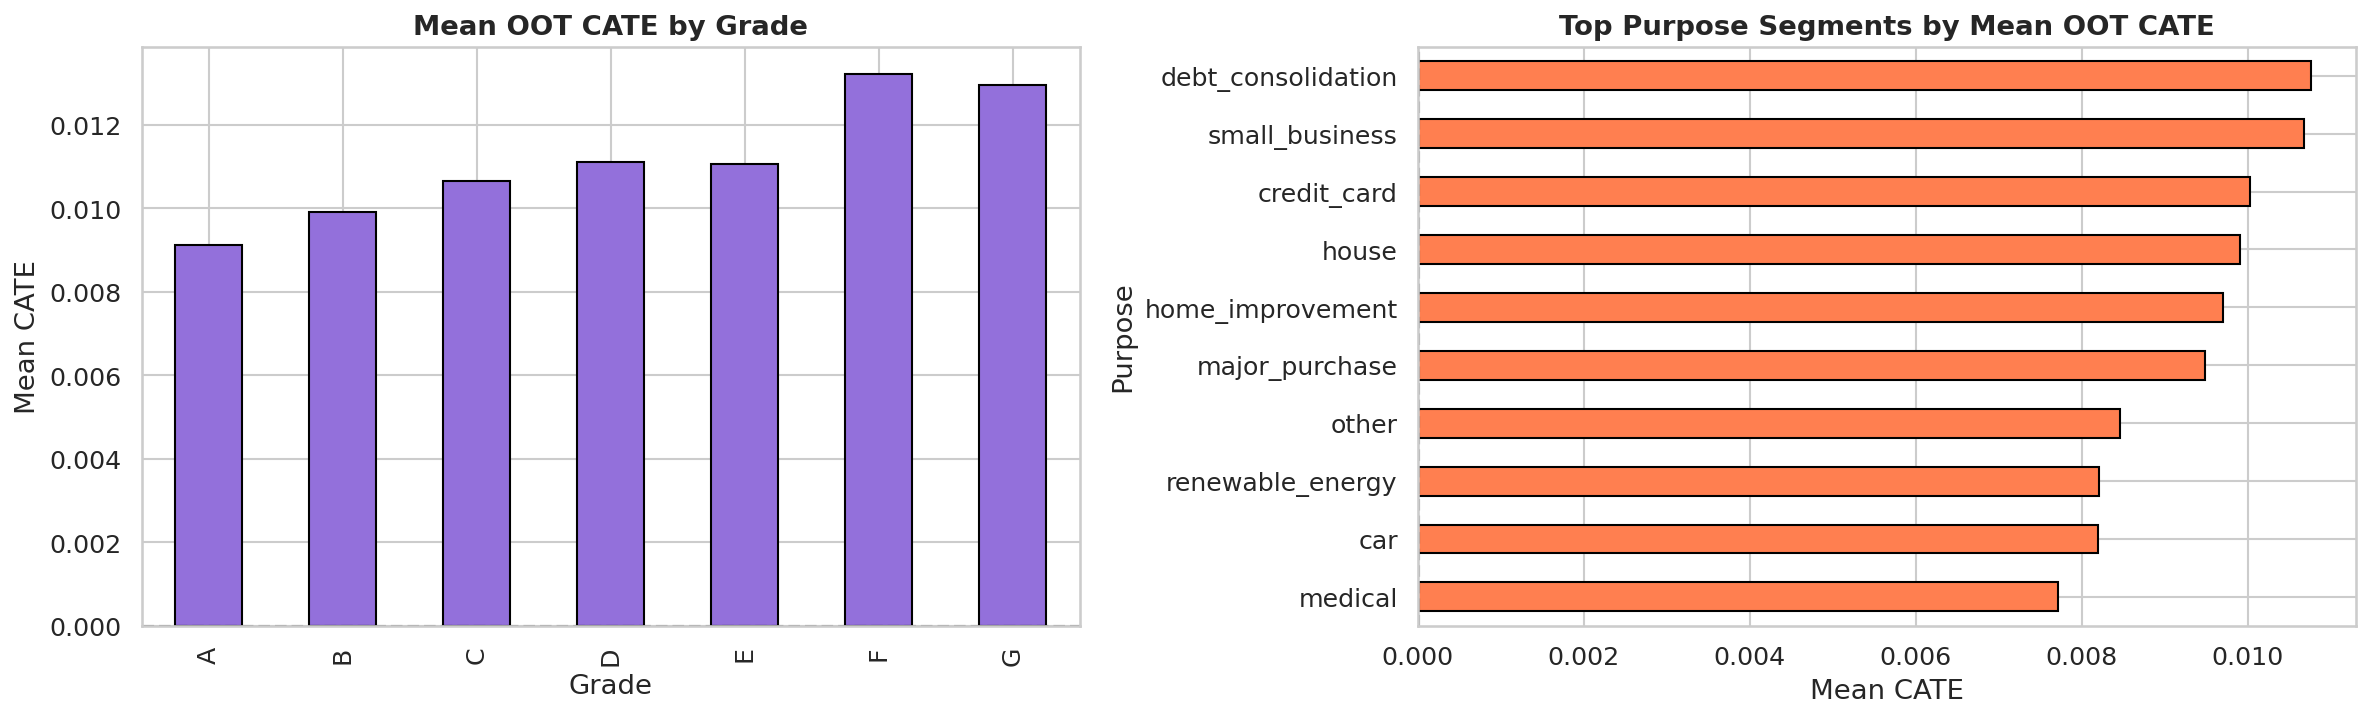
\includegraphics[keepaspectratio,alt={Visualización de heterogeneidad CATE por segmentos del portafolio de crédito.}]{chapters/08-time-survival-causal/../../assets/figures/notebooks/cate_segment_heterogeneity.png}}

}

\caption{\label{fig-cate-heterogeneity}Heterogeneidad del efecto causal
de la tasa de interés por segmentos, estimada con CausalForestDML.}

\end{figure*}%

La figura Figura~\ref{fig-cate-heterogeneity} resume el paso de una
política única a una política segmentada: el efecto de precio no es
homogéneo y, por tanto, tampoco debería serlo la respuesta comercial.

\begin{tcolorbox}[enhanced jigsaw, arc=.35mm, bottomrule=.15mm, bottomtitle=1mm, breakable, colback=white, colbacktitle=quarto-callout-tip-color!10!white, colframe=quarto-callout-tip-color-frame, coltitle=black, left=2mm, leftrule=.75mm, opacityback=0, opacitybacktitle=0.6, rightrule=.15mm, title=\textcolor{quarto-callout-tip-color}{\faLightbulb}\hspace{0.5em}{Interpretación operativa del CATE}, titlerule=0mm, toprule=.15mm, toptitle=1mm]

\begin{itemize}
\tightlist
\item
  \textbf{CATE \textgreater{} 0}: Subir la tasa en ese segmento
  \emph{aumenta} la probabilidad de default --- conviene no subir o
  incluso reducir la tasa.
\item
  \textbf{CATE \textless{} 0}: Subir la tasa no incrementa default o
  puede asociarse a mejor selección adversa --- hay margen para ajustar
  precio.
\item
  \textbf{CATE \(\approx\) 0}: El efecto es nulo --- la tasa no es
  palanca relevante en ese segmento.
\end{itemize}

\end{tcolorbox}

\subsection{Política Causal y Valor
Económico}\label{poluxedtica-causal-y-valor-econuxf3mico}

La estimación CATE permite diseñar \textbf{políticas de precio
segmentadas}: ajustar la tasa de interés en los segmentos donde el
efecto causal es más adverso. La simulación de política sobre el
conjunto OOT estima un ahorro potencial de \textbf{\$41.7M} por
reducción de defaults en segmentos con CATE alto, comparado con la
política uniforme actual.

\begin{table}

\caption{\label{tbl-causal-summary}Resumen de estimación causal: ATE,
CATE y refutaciones}

\centering{

\begin{Shaded}
\begin{Highlighting}[]
\ImportTok{import}\NormalTok{ sys}
\ImportTok{from}\NormalTok{ pathlib }\ImportTok{import}\NormalTok{ Path}

\NormalTok{sys.path.insert(}\DecValTok{0}\NormalTok{, }\BuiltInTok{str}\NormalTok{(Path.cwd().parent }\ControlFlowTok{if}\NormalTok{ Path.cwd().name }\OperatorTok{==} \StringTok{"book"} \ControlFlowTok{else}\NormalTok{ Path.cwd()))}
\ImportTok{from}\NormalTok{ book.\_helpers.load\_artifacts }\ImportTok{import}\NormalTok{ try\_load\_json}

\ImportTok{import}\NormalTok{ pandas }\ImportTok{as}\NormalTok{ pd}

\NormalTok{pipeline }\OperatorTok{=}\NormalTok{ try\_load\_json(}\StringTok{"pipeline\_summary"}\NormalTok{)}
\NormalTok{causal }\OperatorTok{=}\NormalTok{ pipeline.get(}\StringTok{"causal"}\NormalTok{, \{\})}

\NormalTok{rows }\OperatorTok{=}\NormalTok{ [}
\NormalTok{    \{}\StringTok{"Métrica"}\NormalTok{: }\StringTok{"ATE (int\_rate → default)"}\NormalTok{,}
     \StringTok{"Valor"}\NormalTok{: }\SpecialStringTok{f"}\SpecialCharTok{\{}\NormalTok{causal}\SpecialCharTok{.}\NormalTok{get(}\StringTok{\textquotesingle{}ate\textquotesingle{}}\NormalTok{, }\FloatTok{0.00974}\NormalTok{)}\SpecialCharTok{:.5f\}}\SpecialStringTok{"}\NormalTok{,}
     \StringTok{"Interpretación"}\NormalTok{: }\StringTok{"+1pp tasa → +0.974pp probabilidad de default"}\NormalTok{\},}
\NormalTok{    \{}\StringTok{"Métrica"}\NormalTok{: }\StringTok{"CATE medio"}\NormalTok{,}
     \StringTok{"Valor"}\NormalTok{: }\SpecialStringTok{f"}\SpecialCharTok{\{}\NormalTok{causal}\SpecialCharTok{.}\NormalTok{get(}\StringTok{\textquotesingle{}cate\_mean\textquotesingle{}}\NormalTok{, }\FloatTok{0.00974}\NormalTok{)}\SpecialCharTok{:.5f\}}\SpecialStringTok{"}\NormalTok{,}
     \StringTok{"Interpretación"}\NormalTok{: }\StringTok{"Efecto promedio heterogéneo (≈ATE si homogéneo)"}\NormalTok{\},}
\NormalTok{    \{}\StringTok{"Métrica"}\NormalTok{: }\StringTok{"Ahorro potencial (política CATE)"}\NormalTok{,}
     \StringTok{"Valor"}\NormalTok{: }\StringTok{"$41.7M"}\NormalTok{,}
     \StringTok{"Interpretación"}\NormalTok{: }\StringTok{"Reducción de pérdidas por ajuste de tasa segmentado"}\NormalTok{\},}
\NormalTok{    \{}\StringTok{"Métrica"}\NormalTok{: }\StringTok{"Método de identificación"}\NormalTok{,}
     \StringTok{"Valor"}\NormalTok{: }\StringTok{"Backdoor (DoWhy)"}\NormalTok{,}
     \StringTok{"Interpretación"}\NormalTok{: }\StringTok{"Condicional sobre grade, purpose, home\_ownership WOE"}\NormalTok{\},}
\NormalTok{    \{}\StringTok{"Métrica"}\NormalTok{: }\StringTok{"Estimador"}\NormalTok{,}
     \StringTok{"Valor"}\NormalTok{: }\StringTok{"CausalForestDML (EconML)"}\NormalTok{,}
     \StringTok{"Interpretación"}\NormalTok{: }\StringTok{"DML con honest causal forests, 200 árboles"}\NormalTok{\},}
\NormalTok{]}

\NormalTok{pd.DataFrame(rows)}
\end{Highlighting}
\end{Shaded}

}

\end{table}%

\subsection{Refutaciones de DoWhy}\label{refutaciones-de-dowhy}

La robustez del estimado causal se valida mediante tres tests de
refutación estándar (Sharma \& Kiciman, 2020):

\begin{enumerate}
\def\labelenumi{\arabic{enumi}.}
\tightlist
\item
  \textbf{Placebo treatment} (permutación): Se permuta aleatoriamente el
  tratamiento. Si el efecto estimado persiste, la estimación original es
  espuria. El efecto bajo placebo debe ser cercano a cero.
\item
  \textbf{Random common cause}: Se añade un confusor aleatorio. Si el
  efecto cambia significativamente, el modelo es sensible a confusores
  no observados.
\item
  \textbf{Data subset} (80\%): Se re-estima sobre un subconjunto
  aleatorio. La estabilidad del efecto indica robustez ante variaciones
  muestrales.
\end{enumerate}

\begin{tcolorbox}[enhanced jigsaw, arc=.35mm, bottomrule=.15mm, bottomtitle=1mm, breakable, colback=white, colbacktitle=quarto-callout-warning-color!10!white, colframe=quarto-callout-warning-color-frame, coltitle=black, left=2mm, leftrule=.75mm, opacityback=0, opacitybacktitle=0.6, rightrule=.15mm, title=\textcolor{quarto-callout-warning-color}{\faExclamationTriangle}\hspace{0.5em}{Limitaciones de la inferencia observacional}, titlerule=0mm, toprule=.15mm, toptitle=1mm]

Estos resultados son evidencia causal bajo supuestos de identificación
--- no un experimento aleatorizado. La ignorabilidad condicional no es
testable directamente: si existe un confusor no observado (e.g.,
información privada del prestatario no capturada en las covariables), el
ATE estimado podría estar sesgado. Las refutaciones proporcionan
evidencia de plausibilidad, no prueba de causalidad absoluta.

\end{tcolorbox}

\begin{tcolorbox}[enhanced jigsaw, arc=.35mm, bottomrule=.15mm, bottomtitle=1mm, breakable, colback=white, colbacktitle=quarto-callout-tip-color!10!white, colframe=quarto-callout-tip-color-frame, coltitle=black, left=2mm, leftrule=.75mm, opacityback=0, opacitybacktitle=0.6, rightrule=.15mm, title=\textcolor{quarto-callout-tip-color}{\faLightbulb}\hspace{0.5em}{Conexión con el pipeline}, titlerule=0mm, toprule=.15mm, toptitle=1mm]

La estimación CATE alimenta la optimización de portafolio CATE-adjusted
(Capítulo~\ref{sec-cate-portfolio}), donde los préstamos con CATE alto
reciben penalizaciones en la función objetivo. La simulación A/B
(Capítulo~\ref{sec-ab-testing}) valida retrospectivamente si incorporar
esta señal causal mejora el retorno realizado. Los confusores WOE
provienen del feature engineering documentado en
Capítulo~\ref{sec-woe-iv}.

\end{tcolorbox}

\chapter{Simulación A/B: Robusto vs No-Robusto}\label{sec-ab-testing}

\subsection{Motivación: Medir el Valor de la
Robustez}\label{motivaciuxf3n-medir-el-valor-de-la-robustez}

Los capítulos anteriores construyeron un portafolio robusto que utiliza
\texttt{pd\_high} (intervalo conformal superior) en lugar de
\texttt{pd\_point} para la restricción de PD. La pregunta operativa es
directa: \emph{vale la pena la robustez?} Es decir, la estrategia que
incorpora incertidumbre cuantificada genera mejores retornos realizados
que la estrategia que ignora la incertidumbre?

La simulación A/B retroactiva responde esta pregunta aplicando ambas
estrategias al conjunto OOT (2018--2020) y usando los \textbf{defaults
reales} como ground truth. No es un experimento aleatorizado en
producción, pero proporciona evidencia empírica cuantificable sobre el
valor económico de la predicción conformal.

\subsection{Diseño del Experimento
Retroactivo}\label{diseuxf1o-del-experimento-retroactivo}

El framework de A/B testing (\texttt{src/evaluation/ab\_testing.py})
implementa tres componentes:

\subsubsection{1. Análisis de Potencia}\label{anuxe1lisis-de-potencia}

Antes de la simulación, se estima el tamaño muestral mínimo para
detectar un efecto dado:

\begin{equation}\protect\phantomsection\label{eq-power-analysis}{
n_{\text{por grupo}} = \frac{2 \sigma^2 (z_{\alpha/2} + z_\beta)^2}{\delta^2}
}\end{equation}

donde \(\delta\) es el tamaño del efecto esperado, \(\alpha = 0.05\) es
el nivel de significancia y \(\beta = 0.20\) corresponde a una potencia
del 80\%. Con la aproximación conservadora \(\sigma^2 = 0.25\) para
proporciones, el análisis determina si el conjunto OOT (276,869
préstamos) tiene suficiente poder estadístico.

\subsubsection{2. Split Estratificado}\label{split-estratificado}

La asignación control/tratamiento se realiza con \textbf{estratificación
por grade}, garantizando que ambos grupos tengan la misma distribución
de riesgo base:

\begin{Shaded}
\begin{Highlighting}[]
\ImportTok{from}\NormalTok{ src.evaluation.ab\_testing }\ImportTok{import}\NormalTok{ stratified\_split}

\NormalTok{control, treatment }\OperatorTok{=}\NormalTok{ stratified\_split(}
\NormalTok{    df\_test, strata\_col}\OperatorTok{=}\StringTok{"grade"}\NormalTok{, treatment\_ratio}\OperatorTok{=}\FloatTok{0.50}\NormalTok{, seed}\OperatorTok{=}\DecValTok{42}
\NormalTok{)}
\end{Highlighting}
\end{Shaded}

\begin{itemize}
\tightlist
\item
  \textbf{Grupo A (control)}: Asignación de portafolio usando
  \texttt{pd\_point} --- estrategia no robusta.
\item
  \textbf{Grupo B (tratamiento)}: Asignación usando \texttt{pd\_high}
  (conformal upper bound) --- estrategia robusta.
\end{itemize}

\subsubsection{3. Comparación
Estadística}\label{comparaciuxf3n-estaduxedstica}

Los retornos realizados de cada estrategia se comparan mediante tres
métodos:

{\def\LTcaptype{none} % do not increment counter
\begin{longtable}[]{@{}
  >{\raggedright\arraybackslash}p{(\linewidth - 4\tabcolsep) * \real{0.2500}}
  >{\raggedright\arraybackslash}p{(\linewidth - 4\tabcolsep) * \real{0.4062}}
  >{\raggedright\arraybackslash}p{(\linewidth - 4\tabcolsep) * \real{0.3438}}@{}}
\toprule\noalign{}
\begin{minipage}[b]{\linewidth}\raggedright
Método
\end{minipage} & \begin{minipage}[b]{\linewidth}\raggedright
Descripción
\end{minipage} & \begin{minipage}[b]{\linewidth}\raggedright
Supuestos
\end{minipage} \\
\midrule\noalign{}
\endhead
\bottomrule\noalign{}
\endlastfoot
\textbf{Bootstrap} & Remuestreo con reemplazo (1,000 iteraciones) & No
paramétrico \\
\textbf{Permutación} & Intercambio aleatorio de etiquetas A/B & H0:
distribuciones idénticas \\
\textbf{t-test (Welch)} & Comparación de medias con varianzas desiguales
& Normalidad asintótica \\
\end{longtable}
}

El resultado incluye: diferencia de medias, intervalo de confianza al
95\%, p-value y veredicto de significancia.

\subsection{Métricas de
Comparación}\label{muxe9tricas-de-comparaciuxf3n}

Cada estrategia se evalúa sobre múltiples dimensiones:

\begin{table}

\caption{\label{tbl-ab-metrics}Métricas comparadas en la simulación A/B}

\centering{

\begin{Shaded}
\begin{Highlighting}[]
\ImportTok{import}\NormalTok{ pandas }\ImportTok{as}\NormalTok{ pd}

\NormalTok{metrics }\OperatorTok{=}\NormalTok{ [}
\NormalTok{    \{}\StringTok{"Métrica"}\NormalTok{: }\StringTok{"Total return ($)"}\NormalTok{, }\StringTok{"Definición"}\NormalTok{: }\StringTok{"Suma de retornos realizados por préstamo"}\NormalTok{,}
     \StringTok{"Favorece"}\NormalTok{: }\StringTok{"Mayor es mejor"}\NormalTok{\},}
\NormalTok{    \{}\StringTok{"Métrica"}\NormalTok{: }\StringTok{"Default rate (\%)"}\NormalTok{, }\StringTok{"Definición"}\NormalTok{: }\StringTok{"Tasa de incumplimiento en préstamos seleccionados"}\NormalTok{,}
     \StringTok{"Favorece"}\NormalTok{: }\StringTok{"Menor es mejor"}\NormalTok{\},}
\NormalTok{    \{}\StringTok{"Métrica"}\NormalTok{: }\StringTok{"Loans funded (\#)"}\NormalTok{, }\StringTok{"Definición"}\NormalTok{: }\StringTok{"Número de préstamos aprobados"}\NormalTok{,}
     \StringTok{"Favorece"}\NormalTok{: }\StringTok{"Trade{-}off: más funding vs más riesgo"}\NormalTok{\},}
\NormalTok{    \{}\StringTok{"Métrica"}\NormalTok{: }\StringTok{"Avg return per loan ($)"}\NormalTok{, }\StringTok{"Definición"}\NormalTok{: }\StringTok{"Retorno promedio por préstamo seleccionado"}\NormalTok{,}
     \StringTok{"Favorece"}\NormalTok{: }\StringTok{"Mayor es mejor"}\NormalTok{\},}
\NormalTok{    \{}\StringTok{"Métrica"}\NormalTok{: }\StringTok{"Sharpe{-}like ratio"}\NormalTok{, }\StringTok{"Definición"}\NormalTok{: }\StringTok{"Return / volatilidad de retornos"}\NormalTok{,}
     \StringTok{"Favorece"}\NormalTok{: }\StringTok{"Mayor es mejor"}\NormalTok{\},}
\NormalTok{]}

\NormalTok{pd.DataFrame(metrics)}
\end{Highlighting}
\end{Shaded}

}

\end{table}%

\subsection{Interpretación de
Resultados}\label{interpretaciuxf3n-de-resultados}

La estrategia robusta (B) típicamente selecciona \textbf{menos
préstamos} que la no robusta (A), porque
\texttt{pd\_high\ \textgreater{}\ pd\_point} hace que la restricción de
PD sea más estricta. El trade-off fundamental es:

\begin{itemize}
\tightlist
\item
  \textbf{Estrategia A (no robusta)}: Más préstamos aprobados, mayor
  funding, pero mayor exposición a defaults inesperados.
\item
  \textbf{Estrategia B (robusta)}: Menos préstamos aprobados, menor
  funding, pero defaults realizados más cercanos a lo esperado.
\end{itemize}

\begin{tcolorbox}[enhanced jigsaw, arc=.35mm, bottomrule=.15mm, bottomtitle=1mm, breakable, colback=white, colbacktitle=quarto-callout-note-color!10!white, colframe=quarto-callout-note-color-frame, coltitle=black, left=2mm, leftrule=.75mm, opacityback=0, opacitybacktitle=0.6, rightrule=.15mm, title=\textcolor{quarto-callout-note-color}{\faInfo}\hspace{0.5em}{Significancia estadística e intervalo de confianza}, titlerule=0mm, toprule=.15mm, toptitle=1mm]

Si el intervalo de confianza al 95\% de la diferencia no cruza cero, la
diferencia es estadísticamente significativa al nivel \(\alpha = 0.05\).
Esto no garantiza que la diferencia sea \emph{económicamente}
significativa --- el tamaño del efecto y su relevancia operativa deben
evaluarse por separado.

\end{tcolorbox}

\subsection{Atribución por Segmento}\label{atribuciuxf3n-por-segmento}

Además de la comparación global, el framework descompone la diferencia
de retorno por tres dimensiones de atribución:

\begin{itemize}
\tightlist
\item
  \textbf{Por grade}: Permite identificar en qué segmentos de riesgo la
  robustez agrega más valor (típicamente grades C--E, donde la
  incertidumbre es mayor).
\item
  \textbf{Por cohorte temporal}: Revela si la ventaja de la robustez
  varía según el periodo de originación dentro del OOT.
\item
  \textbf{Por monto del préstamo}: Muestra si los préstamos de mayor
  monto se benefician más de la asignación robusta.
\end{itemize}

\begin{table}

\caption{\label{tbl-ab-design-summary}Diseño de la simulación A/B
retroactiva}

\centering{

\begin{Shaded}
\begin{Highlighting}[]
\ImportTok{import}\NormalTok{ pandas }\ImportTok{as}\NormalTok{ pd}

\NormalTok{design }\OperatorTok{=}\NormalTok{ [}
\NormalTok{    \{}\StringTok{"Parámetro"}\NormalTok{: }\StringTok{"Universo de evaluación"}\NormalTok{, }\StringTok{"Valor"}\NormalTok{: }\StringTok{"Conjunto OOT (2018{-}01 a 2020{-}09)"}\NormalTok{\},}
\NormalTok{    \{}\StringTok{"Parámetro"}\NormalTok{: }\StringTok{"Tamaño del universo"}\NormalTok{, }\StringTok{"Valor"}\NormalTok{: }\StringTok{"276,869 préstamos"}\NormalTok{\},}
\NormalTok{    \{}\StringTok{"Parámetro"}\NormalTok{: }\StringTok{"Estratificación"}\NormalTok{, }\StringTok{"Valor"}\NormalTok{: }\StringTok{"Por grade (A{-}{-}G)"}\NormalTok{\},}
\NormalTok{    \{}\StringTok{"Parámetro"}\NormalTok{: }\StringTok{"Ratio control/tratamiento"}\NormalTok{, }\StringTok{"Valor"}\NormalTok{: }\StringTok{"50/50"}\NormalTok{\},}
\NormalTok{    \{}\StringTok{"Parámetro"}\NormalTok{: }\StringTok{"Ground truth"}\NormalTok{, }\StringTok{"Valor"}\NormalTok{: }\StringTok{"Defaults reales observados"}\NormalTok{\},}
\NormalTok{    \{}\StringTok{"Parámetro"}\NormalTok{: }\StringTok{"Métodos estadísticos"}\NormalTok{, }\StringTok{"Valor"}\NormalTok{: }\StringTok{"Bootstrap, permutación, Welch t{-}test"}\NormalTok{\},}
\NormalTok{    \{}\StringTok{"Parámetro"}\NormalTok{: }\StringTok{"Nivel de significancia"}\NormalTok{, }\StringTok{"Valor"}\NormalTok{: }\StringTok{"α = 0.05 (bilateral)"}\NormalTok{\},}
\NormalTok{    \{}\StringTok{"Parámetro"}\NormalTok{: }\StringTok{"PD control (A)"}\NormalTok{, }\StringTok{"Valor"}\NormalTok{: }\StringTok{"pd\_point (estimación puntual calibrada)"}\NormalTok{\},}
\NormalTok{    \{}\StringTok{"Parámetro"}\NormalTok{: }\StringTok{"PD tratamiento (B)"}\NormalTok{, }\StringTok{"Valor"}\NormalTok{: }\StringTok{"pd\_high (bound conformal superior @ 90\%)"}\NormalTok{\},}
\NormalTok{]}

\NormalTok{pd.DataFrame(design)}
\end{Highlighting}
\end{Shaded}

}

\end{table}%

\begin{tcolorbox}[enhanced jigsaw, arc=.35mm, bottomrule=.15mm, bottomtitle=1mm, breakable, colback=white, colbacktitle=quarto-callout-warning-color!10!white, colframe=quarto-callout-warning-color-frame, coltitle=black, left=2mm, leftrule=.75mm, opacityback=0, opacitybacktitle=0.6, rightrule=.15mm, title=\textcolor{quarto-callout-warning-color}{\faExclamationTriangle}\hspace{0.5em}{Limitaciones del diseño retroactivo}, titlerule=0mm, toprule=.15mm, toptitle=1mm]

Esta simulación no es un A/B test aleatorizado en producción. Las
principales limitaciones son: (1) no hay efecto de feedback --- en
producción, aprobar/rechazar un préstamo afecta la composición futura
del portafolio; (2) ambas estrategias se aplican al mismo pool de
candidatos, sin competencia real por funding; (3) si se prueban muchas
variantes de política sin corrección por multiplicidad, la probabilidad
de encontrar mejoras espurias aumenta.

\end{tcolorbox}

\begin{tcolorbox}[enhanced jigsaw, arc=.35mm, bottomrule=.15mm, bottomtitle=1mm, breakable, colback=white, colbacktitle=quarto-callout-tip-color!10!white, colframe=quarto-callout-tip-color-frame, coltitle=black, left=2mm, leftrule=.75mm, opacityback=0, opacitybacktitle=0.6, rightrule=.15mm, title=\textcolor{quarto-callout-tip-color}{\faLightbulb}\hspace{0.5em}{Conexión con el pipeline}, titlerule=0mm, toprule=.15mm, toptitle=1mm]

La simulación A/B cierra el ciclo del pipeline
\textbf{predict-then-optimize}: los intervalos conformal
(Capítulo~\ref{sec-split-conformal}) alimentan la optimización robusta
(Capítulo~\ref{sec-robust-portfolio}), y la simulación A/B valida
retrospectivamente si esa robustez genera valor económico real. Los CATE
de Capítulo~\ref{sec-causal-inference} permiten una variante adicional:
la optimización CATE-adjusted, evaluable con el mismo framework A/B.

\end{tcolorbox}

\chapter{Optimización de
Portafolio}\label{optimizaciuxf3n-de-portafolio}

Este capitulo transforma las predicciones calibradas de PD y los
intervalos de incertidumbre conformal en decisiones concretas de
asignacion de capital. El pipeline completo sigue una arquitectura
\emph{predict-then-optimize} donde cada componente alimenta al
siguiente:

La Tabla~\ref{tbl-portfolio-chapter-overview} resume las secciones y su
contribucion al pipeline.

\begin{longtable}[]{@{}
  >{\raggedright\arraybackslash}p{(\linewidth - 4\tabcolsep) * \real{0.2195}}
  >{\raggedright\arraybackslash}p{(\linewidth - 4\tabcolsep) * \real{0.2683}}
  >{\raggedright\arraybackslash}p{(\linewidth - 4\tabcolsep) * \real{0.5122}}@{}}
\caption{Resumen del capitulo de optimizacion de
portafolio.}\label{tbl-portfolio-chapter-overview}\tabularnewline
\toprule\noalign{}
\begin{minipage}[b]{\linewidth}\raggedright
Seccion
\end{minipage} & \begin{minipage}[b]{\linewidth}\raggedright
Contenido
\end{minipage} & \begin{minipage}[b]{\linewidth}\raggedright
Artefacto principal
\end{minipage} \\
\midrule\noalign{}
\endfirsthead
\toprule\noalign{}
\begin{minipage}[b]{\linewidth}\raggedright
Seccion
\end{minipage} & \begin{minipage}[b]{\linewidth}\raggedright
Contenido
\end{minipage} & \begin{minipage}[b]{\linewidth}\raggedright
Artefacto principal
\end{minipage} \\
\midrule\noalign{}
\endhead
\bottomrule\noalign{}
\endlastfoot
Capítulo~\ref{sec-deterministic-portfolio} & Formulacion LP, Pyomo +
HiGHS & \texttt{portfolio\_allocations.parquet} \\
Capítulo~\ref{sec-robust-portfolio} & Conjuntos de incertidumbre box,
contraparte robusta &
\texttt{portfolio\_robustness\_frontier.parquet} \\
Capítulo~\ref{sec-policy-selection} & Selector economico v3, test A/B de
no-regresion & \texttt{champion\_portfolio\_policy.json} \\
Capítulo~\ref{sec-cate-portfolio} & Ajuste causal (CATE) al retorno
esperado & \texttt{cate\_portfolio\_comparison.parquet} \\
Capítulo~\ref{sec-efficient-frontier} & Frontera de Pareto: riesgo vs
robustez vs retorno & \texttt{portfolio\_robustness\_summary.parquet} \\
\end{longtable}

\begin{tcolorbox}[enhanced jigsaw, arc=.35mm, bottomrule=.15mm, bottomtitle=1mm, breakable, colback=white, colbacktitle=quarto-callout-note-color!10!white, colframe=quarto-callout-note-color-frame, coltitle=black, left=2mm, leftrule=.75mm, opacityback=0, opacitybacktitle=0.6, rightrule=.15mm, title=\textcolor{quarto-callout-note-color}{\faInfo}\hspace{0.5em}{Solver abierto}, titlerule=0mm, toprule=.15mm, toptitle=1mm]

Toda la optimizacion usa \textbf{HiGHS} como solver LP/MILP open-source
(Huangfu \& Hall, 2018), modelado con Pyomo. No se requiere licencia
comercial (Gurobi/CPLEX).

\end{tcolorbox}

\begin{figure*}

\centering{

\pandocbounded{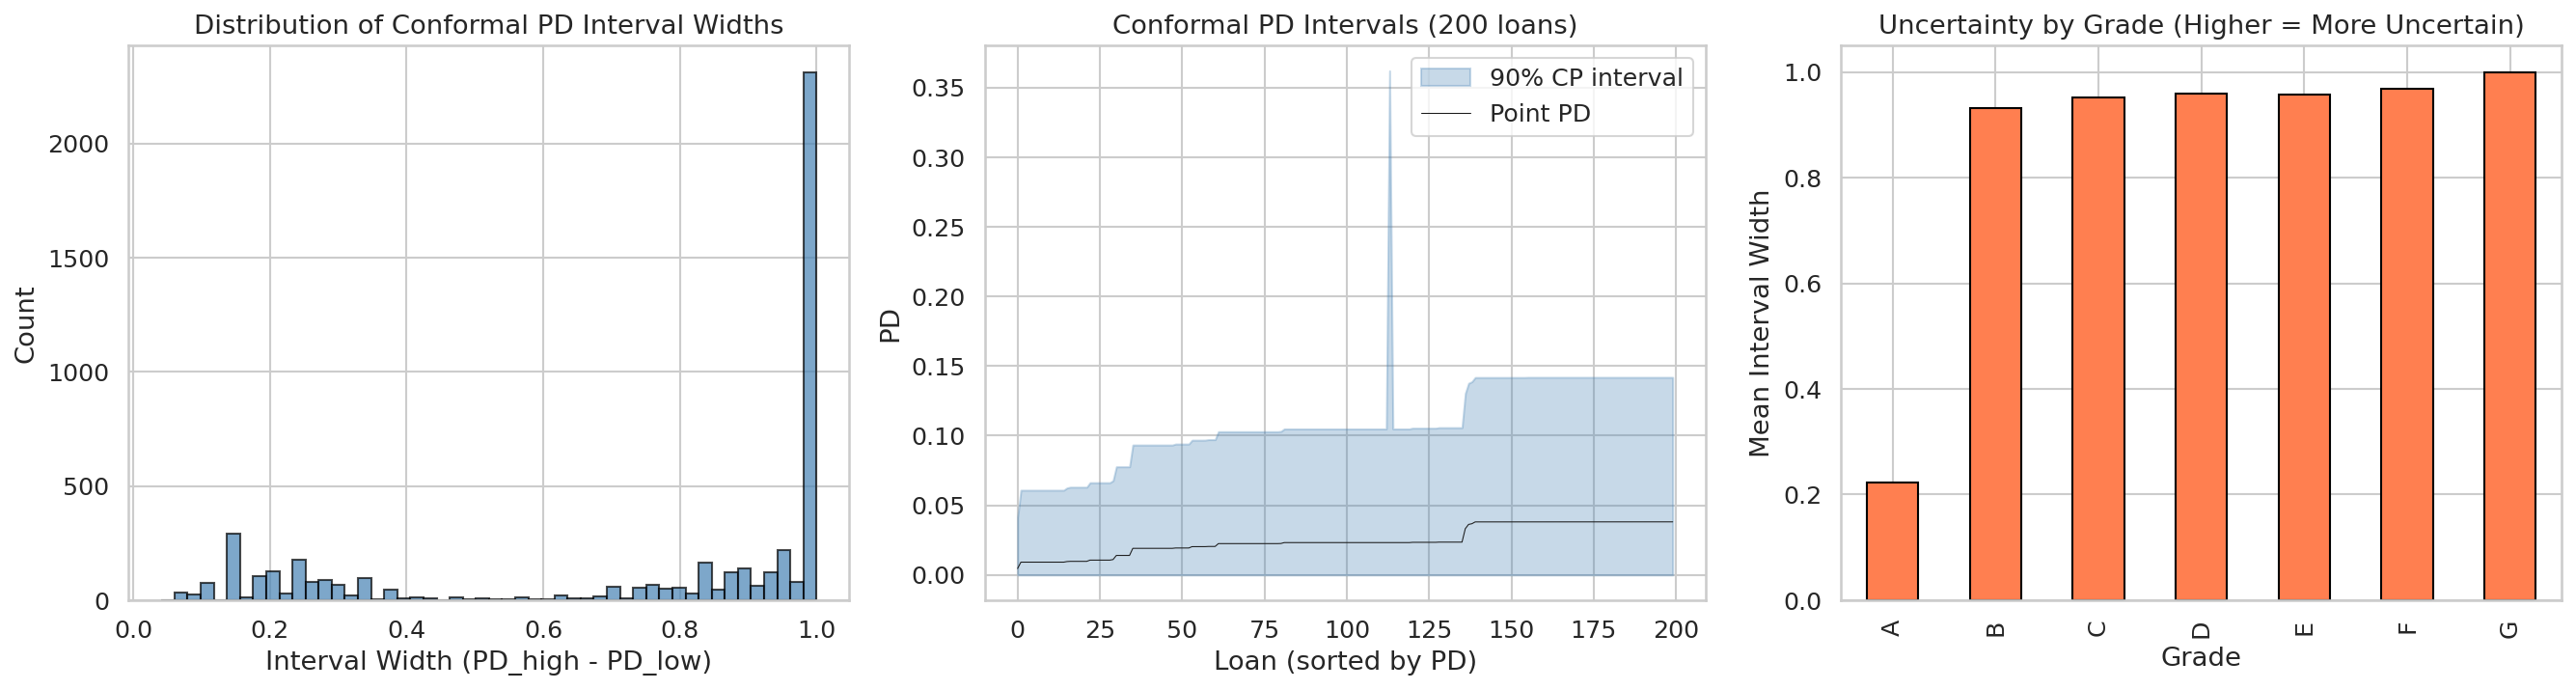
\includegraphics[keepaspectratio,alt={Conjuntos de incertidumbre box usados en la optimización robusta del portafolio.}]{chapters/09-portfolio/../../assets/figures/notebooks/uncertainty_sets.png}}

}

\caption{\label{fig-uncertainty-sets}Visualización de conjuntos de
incertidumbre usados por la capa de optimización robusta para
transformar intervalos conformales en restricciones de decisión.}

\end{figure*}%

La figura Figura~\ref{fig-uncertainty-sets} conecta estadística con OR:
cada intervalo conformal deja de ser una salida descriptiva y se
convierte en una región factible de decisión.

\chapter{Portafolio Determinístico}\label{sec-deterministic-portfolio}

El punto de partida de la optimizacion de portafolio es un programa
lineal (LP) que maximiza el retorno esperado neto de perdida, sujeto a
restricciones de presupuesto, riesgo y diversificacion. Esta formulacion
deterministica usa unicamente la PD puntual ---sin incorporar
incertidumbre--- y sirve como \textbf{baseline} contra el cual se mide
el costo de la robustez.

\subsection{Formulacion matematica}\label{formulacion-matematica}

Sea \(\mathcal{I} = \{1, \dots, n\}\) el conjunto de prestamos
candidatos. Para cada prestamo \(i\) definimos:

\begin{itemize}
\tightlist
\item
  \(x_i \in [0, 1]\): fraccion del prestamo \(i\) a financiar (variable
  de decision),
\item
  \(a_i\): monto del prestamo,
\item
  \(r_i\): tasa de interes (retorno esperado),
\item
  \(\widehat{PD}_i\): probabilidad de default estimada (puntual),
\item
  \(LGD_i\): perdida dado el default (fija en 0.45 para este dataset).
\end{itemize}

El programa lineal determinístico es:

\begin{equation}\protect\phantomsection\label{eq-deterministic-objective}{
\max_{x} \sum_{i \in \mathcal{I}} x_i \cdot a_i \cdot \left( r_i - \widehat{PD}_i \cdot LGD_i \right)
}\end{equation}

sujeto a:

\begin{equation}\protect\phantomsection\label{eq-budget-constraint}{
\sum_{i \in \mathcal{I}} x_i \cdot a_i \leq B
}\end{equation}

\begin{equation}\protect\phantomsection\label{eq-pd-cap-constraint}{
\frac{\sum_{i \in \mathcal{I}} x_i \cdot a_i \cdot \widehat{PD}_i}{\sum_{i \in \mathcal{I}} x_i \cdot a_i} \leq \bar{PD}
}\end{equation}

\begin{equation}\protect\phantomsection\label{eq-concentration-constraint}{
\frac{\sum_{i \in \mathcal{S}_p} x_i \cdot a_i}{\sum_{i \in \mathcal{I}} x_i \cdot a_i} \leq c_{\max}, \quad \forall p \in \mathcal{P}
}\end{equation}

donde \(B\) es el presupuesto total, \(\bar{PD}\) es el techo de PD
ponderada del portafolio (tolerancia al riesgo), \(\mathcal{S}_p\) son
los prestamos del segmento \(p\) (por proposito de credito), y
\(c_{\max}\) es la concentracion maxima permitida por segmento.

\subsection{Parametros de
configuracion}\label{parametros-de-configuracion}

Los valores por defecto se definen en
\texttt{configs/optimization.yaml}:

\begin{longtable}[]{@{}
  >{\raggedright\arraybackslash}p{(\linewidth - 4\tabcolsep) * \real{0.3548}}
  >{\raggedright\arraybackslash}p{(\linewidth - 4\tabcolsep) * \real{0.2258}}
  >{\raggedright\arraybackslash}p{(\linewidth - 4\tabcolsep) * \real{0.4194}}@{}}
\caption{Configuracion del modelo de portafolio
determinístico.}\label{tbl-deterministic-config}\tabularnewline
\toprule\noalign{}
\begin{minipage}[b]{\linewidth}\raggedright
Parametro
\end{minipage} & \begin{minipage}[b]{\linewidth}\raggedright
Valor
\end{minipage} & \begin{minipage}[b]{\linewidth}\raggedright
Descripcion
\end{minipage} \\
\midrule\noalign{}
\endfirsthead
\toprule\noalign{}
\begin{minipage}[b]{\linewidth}\raggedright
Parametro
\end{minipage} & \begin{minipage}[b]{\linewidth}\raggedright
Valor
\end{minipage} & \begin{minipage}[b]{\linewidth}\raggedright
Descripcion
\end{minipage} \\
\midrule\noalign{}
\endhead
\bottomrule\noalign{}
\endlastfoot
\texttt{total\_budget} & \$1,000,000 & Capital total disponible \\
\texttt{max\_concentration} & 25\% & Concentracion maxima por segmento
de proposito \\
\texttt{max\_portfolio\_pd} & 10\% & Techo de PD ponderada del
portafolio \\
\texttt{solver} & HiGHS & Solver LP open-source \\
\texttt{time\_limit} & 300 s & Limite de tiempo del solver \\
\end{longtable}

\subsection{Implementacion en Pyomo}\label{implementacion-en-pyomo}

El modelo se construye con \texttt{build\_portfolio\_model()} en
\texttt{src/optimization/portfolio\_model.py}. Las decisiones son
variables continuas \(x_i \in [0, 1]\) (relajacion LP del problema de
aprobacion binario), lo que permite asignaciones parciales y garantiza
solucion en tiempo polinomial.

\begin{verbatim}
model.x = pyo.Var(model.I, domain=pyo.NonNegativeReals, bounds=(0, 1))
\end{verbatim}

La funcion objetivo (Ecuación~\ref{eq-deterministic-objective}) calcula
el retorno neto como la diferencia entre el ingreso por intereses y la
perdida esperada:

\[
\text{Retorno neto}_i = r_i - \widehat{PD}_i \cdot LGD_i
\]

\begin{tcolorbox}[enhanced jigsaw, arc=.35mm, bottomrule=.15mm, bottomtitle=1mm, breakable, colback=white, colbacktitle=quarto-callout-tip-color!10!white, colframe=quarto-callout-tip-color-frame, coltitle=black, left=2mm, leftrule=.75mm, opacityback=0, opacitybacktitle=0.6, rightrule=.15mm, title=\textcolor{quarto-callout-tip-color}{\faLightbulb}\hspace{0.5em}{Variables continuas vs binarias}, titlerule=0mm, toprule=.15mm, toptitle=1mm]

La relajacion continua \(x_i \in [0, 1]\) produce una cota superior del
problema binario (aprobar/rechazar) y se resuelve ordenes de magnitud
mas rapido. Para 5,000 candidatos, HiGHS resuelve el LP en menos de 2
segundos. El modelo MILP binario (\texttt{build\_binary\_model}) esta
disponible pero no se usa en el pipeline principal.

\end{tcolorbox}

\subsection{Resolucion y artefactos}\label{resolucion-y-artefactos}

El script \texttt{scripts/optimize\_portfolio.py} ejecuta el pipeline
completo:

\begin{enumerate}
\def\labelenumi{\arabic{enumi}.}
\tightlist
\item
  Carga candidatos de \texttt{data/processed/test\_fe.parquet} (hasta
  5,000 por defecto),
\item
  Alinea intervalos conformal por \texttt{id} del prestamo,
\item
  Construye y resuelve el modelo Pyomo con HiGHS,
\item
  Persiste \texttt{portfolio\_allocations.parquet} con la asignacion
  optima.
\end{enumerate}

El artefacto de salida contiene para cada prestamo: la fraccion
asignada, el monto, la PD puntual, los limites conformal y la tasa de
interes. Este resultado alimenta directamente el analisis de escenarios
(mejor caso, esperado, peor caso) implementado en
\texttt{scenario\_analysis()} de
\texttt{src/optimization/robust\_opt.py}.

\begin{tcolorbox}[enhanced jigsaw, arc=.35mm, bottomrule=.15mm, bottomtitle=1mm, breakable, colback=white, colbacktitle=quarto-callout-warning-color!10!white, colframe=quarto-callout-warning-color-frame, coltitle=black, left=2mm, leftrule=.75mm, opacityback=0, opacitybacktitle=0.6, rightrule=.15mm, title=\textcolor{quarto-callout-warning-color}{\faExclamationTriangle}\hspace{0.5em}{Fragilidad del baseline determinístico}, titlerule=0mm, toprule=.15mm, toptitle=1mm]

El portafolio determinístico ignora completamente la incertidumbre de
estimacion. Si la PD real es mayor que la estimada, el portafolio puede
violar su techo de riesgo. Esta fragilidad motiva la formulacion robusta
de Capítulo~\ref{sec-robust-portfolio}.

\end{tcolorbox}

\chapter{Portafolio Robusto con Conjuntos de
Incertidumbre}\label{sec-robust-portfolio}

La formulacion determinística de
Capítulo~\ref{sec-deterministic-portfolio} asume que \(\widehat{PD}_i\)
es conocida con certeza. En la practica, la PD estimada tiene un error
de estimacion que los intervalos conformal cuantifican con garantias
finitas de cobertura (Capítulo~\ref{sec-split-conformal}). Esta seccion
formaliza como convertir esos intervalos en \textbf{conjuntos de
incertidumbre} para optimizacion robusta, siguiendo el marco de
Bertsimas y Sim (2004a).

\subsection{Conjuntos de incertidumbre
box}\label{conjuntos-de-incertidumbre-box}

Para cada prestamo \(i\), la prediccion conformal Mondrian
(Capítulo~\ref{sec-mondrian}) produce un intervalo
\([\underline{PD}_i, \overline{PD}_i]\) con cobertura garantizada al
nivel \(1 - \alpha\) (90\% en nuestra configuracion). El
\textbf{conjunto de incertidumbre box} se define como:

\begin{equation}\protect\phantomsection\label{eq-box-uncertainty}{
\mathcal{U}_i = \left\{ PD_i \in \mathbb{R} : \underline{PD}_i \leq PD_i \leq \overline{PD}_i \right\}
}\end{equation}

La funcion \texttt{build\_box\_uncertainty\_set()} en
\texttt{src/optimization/robust\_opt.py} construye estos conjuntos y
calcula el centro y radio de cada intervalo:

\[
\hat{c}_i = \frac{\underline{PD}_i + \overline{PD}_i}{2}, \qquad \hat{r}_i = \frac{\overline{PD}_i - \underline{PD}_i}{2}
\]

\begin{tcolorbox}[enhanced jigsaw, arc=.35mm, bottomrule=.15mm, bottomtitle=1mm, breakable, colback=white, colbacktitle=quarto-callout-note-color!10!white, colframe=quarto-callout-note-color-frame, coltitle=black, left=2mm, leftrule=.75mm, opacityback=0, opacitybacktitle=0.6, rightrule=.15mm, title=\textcolor{quarto-callout-note-color}{\faInfo}\hspace{0.5em}{Cobertura conformal como garantia de robustez}, titlerule=0mm, toprule=.15mm, toptitle=1mm]

La cobertura conformal al 90\% implica que la PD real de al menos el
90\% de los prestamos cae dentro de \(\mathcal{U}_i\). Este es un
resultado \textbf{distribution-free} que no depende de supuestos
distribucionales --- a diferencia de intervalos bootstrap o bayesianos.

\end{tcolorbox}

\subsection{Contraparte robusta}\label{contraparte-robusta}

El portafolio robusto reemplaza la PD puntual en la restriccion de
riesgo (Ecuación~\ref{eq-pd-cap-constraint}) por una \textbf{PD
efectiva} que incorpora la incertidumbre. La implementacion soporta
multiples politicas de conservadurismo a traves de
\texttt{compute\_effective\_pd()}:

\begin{equation}\protect\phantomsection\label{eq-effective-pd}{
PD_i^{\text{eff}} = \widehat{PD}_i + \gamma \cdot \Delta_i
}\end{equation}

donde \(\Delta_i = \overline{PD}_i - \widehat{PD}_i\) es el ancho hacia
el peor caso y \(\gamma \in [0, 1]\) controla el nivel de robustez:

\begin{longtable}[]{@{}ll@{}}
\caption{Interpretacion del parametro de robustez
\(\gamma\).}\label{tbl-gamma-interpretation}\tabularnewline
\toprule\noalign{}
\(\gamma\) & Interpretacion \\
\midrule\noalign{}
\endfirsthead
\toprule\noalign{}
\(\gamma\) & Interpretacion \\
\midrule\noalign{}
\endhead
\bottomrule\noalign{}
\endlastfoot
0.0 & Sin robustez (equivalente a determinístico) \\
0.10 & Conservadurismo leve \\
0.50 & Proteccion intermedia \\
1.0 & Peor caso total (\(PD_i^{\text{eff}} = \overline{PD}_i\)) \\
\end{longtable}

\subsection{Politicas de PD efectiva}\label{politicas-de-pd-efectiva}

El sistema implementa siete modos de calculo para \(PD_i^{\text{eff}}\),
organizados por sofisticacion creciente:

\begin{enumerate}
\def\labelenumi{\arabic{enumi}.}
\tightlist
\item
  \textbf{\texttt{point\_estimate}}:
  \(PD_i^{\text{eff}} = \widehat{PD}_i\) (baseline).
\item
  \textbf{\texttt{hard\_worst\_case}}:
  \(PD_i^{\text{eff}} = \overline{PD}_i\) (maximo conservadurismo).
\item
  \textbf{\texttt{blended\_uncertainty}}: interpolacion lineal
  (Ecuación~\ref{eq-effective-pd}).
\item
  \textbf{\texttt{capped\_blended\_uncertainty}}: \(\Delta_i\) acotado
  por un cuantil del portafolio.
\item
  \textbf{\texttt{tail\_blended\_uncertainty}}: solo aplica \(\Delta_i\)
  a prestamos en la cola de incertidumbre (cuantil \(q\)).
\item
  \textbf{\texttt{segment\_tail\_blended\_uncertainty}}: cola por
  segmento (grado + plazo + verificacion).
\item
  \textbf{\texttt{segment\_relative\_tail\_blended\_uncertainty}}: cola
  relativa \(\Delta_i / \max(\widehat{PD}_i, 10^{-4})\), por segmento.
\end{enumerate}

La politica seleccionada para el champion actual es
\textbf{\texttt{segment\_relative\_tail\_blended\_uncertainty}} con
\(\gamma = 0.10\), lo que significa que solo los prestamos con ancho
relativo de incertidumbre en la cola superior (por segmento) reciben un
ajuste de robustez.

\subsection{Penalizacion de incertidumbre en el
objetivo}\label{penalizacion-de-incertidumbre-en-el-objetivo}

Ademas de la restriccion de PD, el modelo permite penalizar la
incertidumbre directamente en la funcion objetivo:

\begin{equation}\protect\phantomsection\label{eq-robust-objective}{
\max_{x} \sum_{i} x_i \cdot a_i \cdot \left( r_i - \widehat{PD}_i \cdot LGD_i - \lambda \cdot \Delta_i \cdot LGD_i \right)
}\end{equation}

donde \(\lambda \geq 0\) es la \textbf{aversion a la incertidumbre}
(\texttt{uncertainty\_aversion}). Valores tipicos explorados:
\(\lambda \in \{0.0, 0.1, 0.5, 1.0, 2.0, 3.0\}\).

\subsection{Resultados de la contraparte
robusta}\label{resultados-de-la-contraparte-robusta}

El champion seleccionado presenta los siguientes indicadores de
robustez:

\begin{longtable}[]{@{}ll@{}}
\caption{Metricas de robustez del portafolio
champion.}\label{tbl-robust-metrics}\tabularnewline
\toprule\noalign{}
Metrica & Valor \\
\midrule\noalign{}
\endfirsthead
\toprule\noalign{}
Metrica & Valor \\
\midrule\noalign{}
\endhead
\bottomrule\noalign{}
\endlastfoot
Reduccion de PD en peor caso & \textasciitilde903 bps \\
Price of Robustness & -2.58\% \\
Similitud de asignacion vs baseline & 0.687 (coseno) \\
Breadth score & 0.937 \\
\end{longtable}

\begin{tcolorbox}[enhanced jigsaw, arc=.35mm, bottomrule=.15mm, bottomtitle=1mm, breakable, colback=white, colbacktitle=quarto-callout-tip-color!10!white, colframe=quarto-callout-tip-color-frame, coltitle=black, left=2mm, leftrule=.75mm, opacityback=0, opacitybacktitle=0.6, rightrule=.15mm, title=\textcolor{quarto-callout-tip-color}{\faLightbulb}\hspace{0.5em}{Precio de la robustez como ``prima de seguro''}, titlerule=0mm, toprule=.15mm, toptitle=1mm]

El \emph{Price of Robustness} de -2.58\% significa que el portafolio
robusto sacrifica solo 2.58\% de retorno esperado a cambio de una
reduccion de \textasciitilde903 puntos base en la PD del peor caso. Esta
es la \textbf{prima de seguro} que el portafolio paga por proteccion
contra incertidumbre del modelo.

\end{tcolorbox}

\subsection{Analisis de escenarios}\label{analisis-de-escenarios}

La funcion \texttt{scenario\_analysis()} evalua el portafolio bajo tres
realizaciones de PD:

\[
L_{\text{scenario}} = \sum_i x_i \cdot a_i \cdot PD_i^{\text{scenario}} \cdot LGD_i
\]

donde
\(PD_i^{\text{scenario}} \in \{\underline{PD}_i, \widehat{PD}_i, \overline{PD}_i\}\)
corresponde al mejor caso, esperado y peor caso respectivamente. La
diferencia entre peor y mejor caso cuantifica la \textbf{exposicion
residual a incertidumbre} del portafolio seleccionado.

\chapter{Selección de Política Económica}\label{sec-policy-selection}

Con multiples combinaciones de tolerancia al riesgo (\(\bar{PD}\)), modo
de politica, parametro de robustez (\(\gamma\)) y aversion a la
incertidumbre (\(\lambda\)), el espacio de politicas viables es enorme.
El \textbf{selector economico v3} (\texttt{economic\_actual\_ab\_v3})
automatiza la seleccion de la politica champion mediante un proceso de
tres etapas: evaluacion exhaustiva, test de no-regresion A/B y seleccion
multicriterio.

\subsection{Proceso de seleccion}\label{proceso-de-seleccion}

El script \texttt{scripts/optimize\_portfolio\_tradeoff.py} ejecuta una
busqueda exhaustiva sobre la grilla de configuraciones. Para cada nivel
de tolerancia al riesgo:

\begin{enumerate}
\def\labelenumi{\arabic{enumi}.}
\tightlist
\item
  \textbf{Baseline no robusto}: se resuelve el LP determinístico (PD
  puntual, \(\gamma = 0\), \(\lambda = 0\)).
\item
  \textbf{Candidatos robustos}: se resuelven todas las combinaciones de
  \texttt{(policy\_mode,\ gamma,\ delta\_cap\_quantile,\ tail\_focus\_quantile)}
  \(\times\) \texttt{aversion\_grid}.
\item
  \textbf{Price of Robustness}: se calcula como la diferencia de retorno
  neto entre baseline y candidato robusto.
\item
  \textbf{Retorno realizado}: se computa el retorno \emph{ex-post}
  usando las etiquetas reales de default del set OOT.
\end{enumerate}

\subsection{Test A/B de no-regresion}\label{sec-ab-no-regression}

El test A/B no es un A/B test experimental online, sino una evaluacion
retroactiva: dado que conocemos los defaults reales del periodo OOT
(2018--2020), se compara el retorno realizado del portafolio robusto
contra el baseline no robusto.

La condicion de no-regresion es:

\begin{equation}\protect\phantomsection\label{eq-ab-no-regression}{
R_{\text{robusto}}^{\text{realizado}} \geq R_{\text{baseline}}^{\text{realizado}} - 0.05 \cdot |R_{\text{baseline}}^{\text{realizado}}|
}\end{equation}

Es decir, el portafolio robusto puede perder hasta un 5\% del retorno
realizado del baseline sin ser descartado. Este margen reconoce que la
robustez tiene un costo, pero limita cuanto puede costar.

\subsection{Politica champion
seleccionada}\label{politica-champion-seleccionada}

El selector economico v3 eligio la siguiente politica como champion:

\begin{longtable}[]{@{}ll@{}}
\caption{Politica champion seleccionada por el selector economico
v3.}\label{tbl-champion-policy}\tabularnewline
\toprule\noalign{}
Parametro & Valor \\
\midrule\noalign{}
\endfirsthead
\toprule\noalign{}
Parametro & Valor \\
\midrule\noalign{}
\endhead
\bottomrule\noalign{}
\endlastfoot
\texttt{risk\_tolerance} & 0.18 \\
\texttt{uncertainty\_aversion} (\(\lambda\)) & 0.10 \\
\texttt{policy\_mode} &
\texttt{segment\_relative\_tail\_blended\_uncertainty} \\
\texttt{gamma} & 0.10 \\
\texttt{tail\_focus\_quantile} & 0.75 \\
\texttt{delta\_cap\_quantile} & 1.0 \\
A/B no-regresion & PASS \\
\end{longtable}

\begin{tcolorbox}[enhanced jigsaw, arc=.35mm, bottomrule=.15mm, bottomtitle=1mm, breakable, colback=white, colbacktitle=quarto-callout-note-color!10!white, colframe=quarto-callout-note-color-frame, coltitle=black, left=2mm, leftrule=.75mm, opacityback=0, opacitybacktitle=0.6, rightrule=.15mm, title=\textcolor{quarto-callout-note-color}{\faInfo}\hspace{0.5em}{Interpretacion de la politica champion}, titlerule=0mm, toprule=.15mm, toptitle=1mm]

La politica \texttt{segment\_relative\_tail\_blended\_uncertainty} con
\(\gamma = 0.10\) aplica un ajuste de robustez solo al 25\% superior de
prestamos por ancho relativo de incertidumbre, dentro de cada segmento
(grado \(\times\) plazo \(\times\) verificacion). Esto significa que los
prestamos con PD bien estimada no reciben penalizacion, mientras que
aquellos donde el modelo tiene mayor incertidumbre relativa si la
reciben.

\end{tcolorbox}

\subsection{Alternativas de
investigacion}\label{alternativas-de-investigacion}

El selector evalua cuatro estrategias de seleccion alternativas para
comparacion academica:

\begin{longtable}[]{@{}
  >{\raggedright\arraybackslash}p{(\linewidth - 6\tabcolsep) * \real{0.1724}}
  >{\raggedright\arraybackslash}p{(\linewidth - 6\tabcolsep) * \real{0.3276}}
  >{\raggedright\arraybackslash}p{(\linewidth - 6\tabcolsep) * \real{0.2759}}
  >{\raggedright\arraybackslash}p{(\linewidth - 6\tabcolsep) * \real{0.2241}}@{}}
\caption{Alternativas de seleccion de politica para
investigacion.}\label{tbl-research-alternatives}\tabularnewline
\toprule\noalign{}
\begin{minipage}[b]{\linewidth}\raggedright
Selector
\end{minipage} & \begin{minipage}[b]{\linewidth}\raggedright
Criterio principal
\end{minipage} & \begin{minipage}[b]{\linewidth}\raggedright
Risk tolerance
\end{minipage} & \begin{minipage}[b]{\linewidth}\raggedright
Policy mode
\end{minipage} \\
\midrule\noalign{}
\endfirsthead
\toprule\noalign{}
\begin{minipage}[b]{\linewidth}\raggedright
Selector
\end{minipage} & \begin{minipage}[b]{\linewidth}\raggedright
Criterio principal
\end{minipage} & \begin{minipage}[b]{\linewidth}\raggedright
Risk tolerance
\end{minipage} & \begin{minipage}[b]{\linewidth}\raggedright
Policy mode
\end{minipage} \\
\midrule\noalign{}
\endhead
\bottomrule\noalign{}
\endlastfoot
\textbf{promotion\_first} & Maximiza retorno realizado & 0.16 &
\texttt{tail\_blended\_uncertainty} \\
\textbf{robustness\_aware} & Retorno \(\times \sqrt{\gamma}\) & 0.16 &
\texttt{tail\_blended\_uncertainty} \\
\textbf{balanced} & Retorno + \(\gamma\) alto & 0.16 &
\texttt{tail\_blended\_uncertainty} \\
\textbf{guardrail} & PoR \(\geq\) -25\% + retorno & 0.14 &
\texttt{hard\_worst\_case} \\
\end{longtable}

La estrategia \texttt{robustness\_aware} pondera el retorno realizado
por \(\sqrt{\gamma}\), incentivando politicas que realmente usen la
informacion de incertidumbre (no trivialmente \(\gamma = 0\)). La
estrategia \texttt{guardrail} impone un piso al Price of Robustness para
evitar politicas extremadamente conservadoras.

\subsection{Breadth score}\label{breadth-score}

Para verificar que la politica robusta no colapsa el portafolio a un
subconjunto degenerado de prestamos, se calcula un \textbf{breadth
score} compuesto:

\begin{equation}\protect\phantomsection\label{eq-breadth-score}{
\text{Breadth} = w_1 \cdot \frac{n_{\text{funded}}^{\text{robusto}}}{n_{\text{funded}}^{\text{baseline}}} + w_2 \cdot \frac{\text{allocated}^{\text{robusto}}}{\text{allocated}^{\text{baseline}}} + w_3 \cdot \text{sim}(\mathbf{x}^{\text{robusto}}, \mathbf{x}^{\text{baseline}})
}\end{equation}

con pesos \(w_1 = 0.50\), \(w_2 = 0.30\), \(w_3 = 0.20\) y similitud
coseno entre vectores de asignacion. El umbral minimo es 0.93; el
champion actual alcanza \textbf{0.937}, indicando que la politica
robusta mantiene un portafolio amplio y diversificado.

\begin{tcolorbox}[enhanced jigsaw, arc=.35mm, bottomrule=.15mm, bottomtitle=1mm, breakable, colback=white, colbacktitle=quarto-callout-warning-color!10!white, colframe=quarto-callout-warning-color-frame, coltitle=black, left=2mm, leftrule=.75mm, opacityback=0, opacitybacktitle=0.6, rightrule=.15mm, title=\textcolor{quarto-callout-warning-color}{\faExclamationTriangle}\hspace{0.5em}{Configuracion como template}, titlerule=0mm, toprule=.15mm, toptitle=1mm]

Los archivos YAML en \texttt{configs/} son \textbf{templates} con
valores por defecto. La politica efectiva en produccion es el artefacto
\texttt{models/champion\_portfolio\_policy.json}, que captura la
decision del selector economico con todos los parametros resueltos y las
metricas de seleccion.

\end{tcolorbox}

\chapter{Portafolio Ajustado por CATE}\label{sec-cate-portfolio}

El portafolio determinístico y el robusto utilizan retornos esperados
basados unicamente en la tasa de interes y la perdida esperada. Sin
embargo, la inferencia causal (Capítulo~\ref{sec-causal-inference})
estima el \textbf{efecto heterogeneo del tratamiento} (CATE) para cada
prestamo, lo que permite ajustar la expectativa de retorno incorporando
informacion causal. Esta seccion describe como el CATE modifica la
funcion objetivo de la optimizacion.

\subsection{Integracion del CATE en el
retorno}\label{integracion-del-cate-en-el-retorno}

Sea \(\tau_i\) el CATE estimado para el prestamo \(i\), que representa
el efecto causal diferencial de la politica de aprobacion sobre la
probabilidad de repago. El retorno ajustado es:

\begin{equation}\protect\phantomsection\label{eq-cate-return}{
\text{Retorno}_i^{\text{CATE}} = r_i - \widehat{PD}_i \cdot LGD_i + \delta \cdot \tau_i
}\end{equation}

donde \(\delta\) es un factor de escala (por defecto \(\delta = -1\),
indicando que un CATE positivo reduce el riesgo y mejora el retorno). La
funcion \texttt{build\_cate\_adjusted\_portfolio()} en
\texttt{src/optimization/causal\_portfolio.py} resuelve el LP con este
retorno modificado y lo compara contra el baseline sin CATE.

\subsection{Alineacion de CATE al set
OOT}\label{alineacion-de-cate-al-set-oot}

Un desafio tecnico importante es que los estimados CATE se producen
originalmente sobre el set de entrenamiento (1.34M prestamos), mientras
que la optimizacion opera sobre el set OOT (276K prestamos) con cero
solapamiento de IDs. El script
\texttt{scripts/optimize\_cate\_portfolio.py} implementa una cascada de
estrategias de alineacion:

\begin{enumerate}
\def\labelenumi{\arabic{enumi}.}
\tightlist
\item
  \textbf{OOT directo}: si existe \texttt{cate\_estimates\_oot.parquet},
  se hace join por \texttt{id}.
\item
  \textbf{Training fallback}: join por \texttt{id} con CATE del set de
  entrenamiento.
\item
  \textbf{Grade mediana}: para IDs sin match, se imputa la mediana de
  CATE por grado crediticio.
\item
  \textbf{Zero-fill}: prestamos restantes reciben CATE = 0 (efecto
  neutral).
\end{enumerate}

\subsection{Shrinkage del CATE}\label{shrinkage-del-cate}

Los estimados CATE crudos pueden contener senales ruidosas o valores
extremos. Para mitigar esto, se aplica un procedimiento de
\textbf{shrinkage} antes de la optimizacion:

\begin{enumerate}
\def\labelenumi{\arabic{enumi}.}
\tightlist
\item
  \textbf{Winsorization}: se recortan los valores por debajo del
  percentil 5 y por encima del percentil 95.
\item
  \textbf{Shrinkage a mediana de segmento}:
  \(\tau_i^{\text{shrunk}} = 0.5 \cdot \tau_i^{\text{clip}} + 0.5 \cdot \tilde{\tau}_{\text{seg}(i)}\),
  donde \(\tilde{\tau}_{\text{seg}(i)}\) es la mediana del CATE en el
  segmento (grado \(\times\) plazo \(\times\) verificacion).
\item
  \textbf{Piso de senal debil}: valores con
  \(|\tau_i^{\text{shrunk}}| < \text{floor}\) se anulan a cero.
\end{enumerate}

\subsection{Resultados: CATE crudo vs
shrunk}\label{resultados-cate-crudo-vs-shrunk}

El script ejecuta ambas versiones (CATE crudo y shrunk) para cuantificar
el efecto del shrinkage:

\begin{longtable}[]{@{}llll@{}}
\caption{Comparacion de portafolios baseline vs
CATE-ajustado.}\label{tbl-cate-comparison}\tabularnewline
\toprule\noalign{}
Escenario & Retorno baseline & Retorno CATE-ajustado & Diferencia \\
\midrule\noalign{}
\endfirsthead
\toprule\noalign{}
Escenario & Retorno baseline & Retorno CATE-ajustado & Diferencia \\
\midrule\noalign{}
\endhead
\bottomrule\noalign{}
\endlastfoot
CATE crudo & \$57,094 & \$57,350 & +\$257 (+0.45\%) \\
CATE shrunk & \$57,094 & \$54,540 & -\$2,554 (-4.47\%) \\
\end{longtable}

\begin{tcolorbox}[enhanced jigsaw, arc=.35mm, bottomrule=.15mm, bottomtitle=1mm, breakable, colback=white, colbacktitle=quarto-callout-tip-color!10!white, colframe=quarto-callout-tip-color-frame, coltitle=black, left=2mm, leftrule=.75mm, opacityback=0, opacitybacktitle=0.6, rightrule=.15mm, title=\textcolor{quarto-callout-tip-color}{\faLightbulb}\hspace{0.5em}{Interpretacion del efecto del shrinkage}, titlerule=0mm, toprule=.15mm, toptitle=1mm]

El CATE crudo muestra una mejora marginal (+\$257), mientras que el CATE
shrunk reduce el retorno (-\$2,554). Esto es esperado: el shrinkage
elimina senal ruidosa que artificialmente inflaba el retorno ajustado,
produciendo una estimacion mas conservadora pero mas confiable del
efecto causal real.

\end{tcolorbox}

\subsection{Criterio de promocion}\label{criterio-de-promocion}

La politica CATE-ajustada se promueve a candidata operativa solo si
cumple dos condiciones:

\begin{enumerate}
\def\labelenumi{\arabic{enumi}.}
\tightlist
\item
  El retorno del portafolio CATE-ajustado \(\geq\) retorno baseline.
\item
  El numero de prestamos financiados \(\geq 90\%\) del baseline.
\end{enumerate}

Si no se cumplen, la politica queda en modo
\texttt{research\_only\_fallback} --- util para analisis academico pero
no para produccion. El artefacto
\texttt{models/cate\_portfolio\_status.json} registra la decision y las
metricas de evaluacion.

\begin{tcolorbox}[enhanced jigsaw, arc=.35mm, bottomrule=.15mm, bottomtitle=1mm, breakable, colback=white, colbacktitle=quarto-callout-note-color!10!white, colframe=quarto-callout-note-color-frame, coltitle=black, left=2mm, leftrule=.75mm, opacityback=0, opacitybacktitle=0.6, rightrule=.15mm, title=\textcolor{quarto-callout-note-color}{\faInfo}\hspace{0.5em}{Conexion con inferencia causal}, titlerule=0mm, toprule=.15mm, toptitle=1mm]

Los estimados CATE provienen de Causal Forests (ver
Capítulo~\ref{sec-causal-inference}). La calidad de la integracion
causal depende directamente de la identificabilidad del efecto y la
cobertura del overlap entre tratados y controles. Las limitaciones de la
estimacion causal se propagan a la optimizacion de portafolio.

\end{tcolorbox}

\chapter{Frontera Eficiente de Robustez}\label{sec-efficient-frontier}

Las secciones anteriores presentan la formulacion del portafolio robusto
y la seleccion de la politica champion. Esta seccion analiza la
\textbf{frontera de Pareto} que emerge al explorar exhaustivamente el
espacio de configuraciones, cuantificando el trade-off entre retorno
esperado, proteccion ante el peor caso y costo de la robustez.

\subsection{Espacio de busqueda}\label{espacio-de-busqueda}

El script \texttt{scripts/optimize\_portfolio\_tradeoff.py} evalua una
grilla tridimensional de configuraciones:

\begin{itemize}
\tightlist
\item
  \textbf{Tolerancia al riesgo} (\(\bar{PD}\)): 9 niveles de 0.05 a
  0.20.
\item
  \textbf{Aversion a la incertidumbre} (\(\lambda\)): 7 niveles de 0.0 a
  3.0.
\item
  \textbf{Modos de politica}: 7 modos \(\times\) multiples combinaciones
  de \(\gamma\), \texttt{delta\_cap\_quantile} y
  \texttt{tail\_focus\_quantile}.
\end{itemize}

En total, el barrido exhaustivo evalua hasta \textbf{6,941
configuraciones de politica} (dependiendo del perfil de grilla
seleccionado). Para cada configuracion, se resuelve el LP completo con
HiGHS y se computan las metricas de robustez.

\subsection{Curva de Price of
Robustness}\label{curva-de-price-of-robustness}

El Price of Robustness (PoR) mide la fraccion de retorno que el
portafolio sacrifica por proteccion:

\begin{equation}\protect\phantomsection\label{eq-price-of-robustness}{
\text{PoR}(\%) = \frac{R_{\text{baseline}} - R_{\text{robusto}}}{|R_{\text{baseline}}|} \times 100
}\end{equation}

La curva de PoR en funcion de \(\gamma\) tiene forma convexa: robustez
marginal es barata (primeros puntos base de proteccion cuestan poco
retorno), pero la proteccion total (\(\gamma = 1.0\)) es
desproporcionadamente costosa. El champion seleccionado en
Capítulo~\ref{sec-policy-selection} opera en la zona de bajo costo
marginal con un PoR de solo -2.58\%.

\subsection{Frontera de Pareto}\label{frontera-de-pareto}

La frontera de Pareto se define como el conjunto de politicas donde no
es posible mejorar una metrica sin empeorar otra. En nuestro contexto,
las metricas son:

\begin{enumerate}
\def\labelenumi{\arabic{enumi}.}
\tightlist
\item
  \textbf{Retorno realizado} (maximizar): retorno \emph{ex-post} con
  defaults reales del OOT.
\item
  \textbf{Reduccion de PD en peor caso} (maximizar): diferencia en PD
  ponderada bajo el escenario \(\overline{PD}_i\).
\item
  \textbf{Breadth score} (maximizar): diversificacion del portafolio
  respecto al baseline.
\end{enumerate}

La Tabla~\ref{tbl-frontier-example} muestra las politicas
Pareto-dominantes a lo largo de la frontera:

\begin{longtable}[]{@{}
  >{\raggedright\arraybackslash}p{(\linewidth - 8\tabcolsep) * \real{0.2877}}
  >{\raggedright\arraybackslash}p{(\linewidth - 8\tabcolsep) * \real{0.1233}}
  >{\raggedright\arraybackslash}p{(\linewidth - 8\tabcolsep) * \real{0.3562}}
  >{\raggedright\arraybackslash}p{(\linewidth - 8\tabcolsep) * \real{0.1233}}
  >{\raggedright\arraybackslash}p{(\linewidth - 8\tabcolsep) * \real{0.1096}}@{}}
\caption{Zonas de la frontera de
robustez.}\label{tbl-frontier-example}\tabularnewline
\toprule\noalign{}
\begin{minipage}[b]{\linewidth}\raggedright
Zona de la frontera
\end{minipage} & \begin{minipage}[b]{\linewidth}\raggedright
PoR (\%)
\end{minipage} & \begin{minipage}[b]{\linewidth}\raggedright
Reduccion worst-PD (bps)
\end{minipage} & \begin{minipage}[b]{\linewidth}\raggedright
Breadth
\end{minipage} & \begin{minipage}[b]{\linewidth}\raggedright
Perfil
\end{minipage} \\
\midrule\noalign{}
\endfirsthead
\toprule\noalign{}
\begin{minipage}[b]{\linewidth}\raggedright
Zona de la frontera
\end{minipage} & \begin{minipage}[b]{\linewidth}\raggedright
PoR (\%)
\end{minipage} & \begin{minipage}[b]{\linewidth}\raggedright
Reduccion worst-PD (bps)
\end{minipage} & \begin{minipage}[b]{\linewidth}\raggedright
Breadth
\end{minipage} & \begin{minipage}[b]{\linewidth}\raggedright
Perfil
\end{minipage} \\
\midrule\noalign{}
\endhead
\bottomrule\noalign{}
\endlastfoot
Agresiva & 0 -- -1\% & 0 -- 200 & \(> 0.98\) & Casi identico al
baseline \\
Balanceada & -1\% -- -5\% & 200 -- 900 & 0.93 -- 0.98 & Trade-off
optimo \\
Conservadora & -5\% -- -15\% & 900 -- 2,000 & 0.85 -- 0.93 & Proteccion
fuerte \\
Extrema & \(< -15\%\) & \(> 2,000\) & \(< 0.85\) & Portafolio
colapsado \\
\end{longtable}

El champion actual (\(\gamma = 0.10\), \(\lambda = 0.10\), PoR =
-2.58\%, \textasciitilde903 bps de reduccion) se ubica firmemente en la
\textbf{zona balanceada}, donde el costo marginal de la robustez es bajo
y la diversificacion del portafolio se mantiene alta.

\subsection{Dimensiones del trade-off}\label{dimensiones-del-trade-off}

El analisis de la frontera revela tres dimensiones del trade-off:

\begin{enumerate}
\def\labelenumi{\arabic{enumi}.}
\tightlist
\item
  \textbf{Retorno vs proteccion}: la curva clasica de PoR. Mayor
  \(\gamma\) protege mas pero cuesta mas retorno.
\item
  \textbf{Volumen vs conservadurismo}: tolerancias al riesgo mas bajas
  (\(\bar{PD} = 0.06\)) rechazan mas prestamos, reduciendo el volumen
  financiado. El piso de utilizacion de presupuesto
  (\texttt{min\_budget\_utilization\ =\ 0.05}) evita soluciones
  degeneradas a niveles estrictos de riesgo.
\item
  \textbf{Granularidad del ajuste}: las politicas \texttt{segment\_*}
  son mas selectivas que \texttt{blended\_uncertainty} global,
  penalizando solo donde la incertidumbre relativa es alta. Esto permite
  mayor robustez sin sacrificio excesivo de retorno.
\end{enumerate}

\begin{tcolorbox}[enhanced jigsaw, arc=.35mm, bottomrule=.15mm, bottomtitle=1mm, breakable, colback=white, colbacktitle=quarto-callout-note-color!10!white, colframe=quarto-callout-note-color-frame, coltitle=black, left=2mm, leftrule=.75mm, opacityback=0, opacitybacktitle=0.6, rightrule=.15mm, title=\textcolor{quarto-callout-note-color}{\faInfo}\hspace{0.5em}{Frontera como herramienta de gobernanza}, titlerule=0mm, toprule=.15mm, toptitle=1mm]

La frontera de robustez no solo es un resultado analitico --- es una
herramienta de decision para el comite de riesgo. Permite comunicar
explicitamente: ``por cada punto porcentual adicional de proteccion, el
portafolio sacrifica \$X de retorno''. Esto transforma la decision de
nivel de robustez en una decision economica cuantificable, no una
eleccion subjetiva.

\end{tcolorbox}

\subsection{Conexion con el pipeline
completo}\label{conexion-con-el-pipeline-completo}

Los artefactos generados por la frontera alimentan multiples componentes
downstream:

\begin{itemize}
\tightlist
\item
  \textbf{\texttt{portfolio\_robustness\_frontier.parquet}}: todas las
  configuraciones evaluadas con sus metricas.
\item
  \textbf{\texttt{portfolio\_robustness\_summary.parquet}}: resumen por
  nivel de tolerancia al riesgo (mejor robusto vs baseline).
\item
  \textbf{\texttt{champion\_portfolio\_policy.json}}: la politica
  promovida tras pasar el test A/B (Sección~\ref{sec-ab-no-regression}).
\item
  \textbf{\texttt{portfolio\_research\_policy.json}}: las cuatro
  alternativas de investigacion (Tabla~\ref{tbl-research-alternatives}).
\end{itemize}

Estos artefactos son consumidos por el dashboard Streamlit para
visualizacion interactiva, por el reporte MRM para validacion
regulatoria, y por la simulacion A/B retroactiva
(\texttt{scripts/simulate\_ab\_test.py}) para evaluar robustez en
condiciones mas realistas.

\chapter{IFRS9 y Gobernanza del
Modelo}\label{ifrs9-y-gobernanza-del-modelo}

Este capítulo conecta los modelos de riesgo crediticio con sus
consecuencias contables y regulatorias. IFRS9 traduce PD, LGD y EAD en
provisiones (ECL) bajo múltiples escenarios macroeconómicos, mientras
que la gobernanza asegura que el sistema sea confiable, justo y
auditable a lo largo del tiempo.

\subsection{Pipeline ECL Completo}\label{pipeline-ecl-completo}

El siguiente diagrama muestra cómo fluye la información desde los
modelos hasta las provisiones y la gobernanza:

\begin{figure*}

\begin{figure}[H]

{\centering \pandocbounded{\includegraphics[keepaspectratio,alt={Figura de staging y SICR conformal para el bloque IFRS9.}]{chapters/10-ifrs9-governance/../../assets/figures/publication/p2_fig4_sicr_grid.png}}

}

\caption{Grid editorial de SICR y staging conformal del carril IFRS9.}

\end{figure}%

\end{figure*}%

\subsection{Resumen de Métricas
Clave}\label{resumen-de-muxe9tricas-clave}

\begin{longtable}[]{@{}lll@{}}
\caption{Resumen de resultados IFRS9 y
gobernanza}\label{tbl-ifrs9-summary}\tabularnewline
\toprule\noalign{}
Métrica & Valor & Sección \\
\midrule\noalign{}
\endfirsthead
\toprule\noalign{}
Métrica & Valor & Sección \\
\midrule\noalign{}
\endhead
\bottomrule\noalign{}
\endlastfoot
ECL Baseline & \$1,003M & Capítulo~\ref{sec-ecl-calculation} \\
ECL Severe & \$1,799M & Capítulo~\ref{sec-scenario-analysis} \\
Uplift Severe & +79.3\% & Capítulo~\ref{sec-scenario-analysis} \\
SICR \(t^*\) conformal & 0.30 (F1=0.2515) &
Capítulo~\ref{sec-sicr-signal} \\
ECL adicional SICR & \$56.6M & Capítulo~\ref{sec-sicr-signal} \\
Sensibilidad \(\alpha\) & ECL +22\% (90\%→99\%) &
Capítulo~\ref{sec-sensitivity-stress} \\
Fairness & 6/6 PASS & Capítulo~\ref{sec-mrm} \\
\end{longtable}

\chapter{Cálculo de ECL}\label{sec-ecl-calculation}

\subsection{La Fórmula Central de
IFRS9}\label{la-fuxf3rmula-central-de-ifrs9}

La \textbf{Expected Credit Loss} (ECL) es la métrica contable que
traduce modelos de riesgo en provisiones monetarias. Bajo IFRS9, cada
préstamo contribuye al total de provisiones según:

\begin{equation}\protect\phantomsection\label{eq-ecl-formula}{
\text{ECL}_i = \text{PD}_i^{\text{eff}} \times \text{LGD}_i \times \text{EAD}_i \times \text{DF}
}\end{equation}

donde:

\begin{itemize}
\tightlist
\item
  \(\text{PD}_i^{\text{eff}}\) es la probabilidad de default efectiva
  según el stage del préstamo,
\item
  \(\text{LGD}_i\) es la pérdida dado el default (45\% en nuestro
  escenario base),
\item
  \(\text{EAD}_i\) es la exposición al momento del default (monto del
  préstamo),
\item
  \(\text{DF} = \frac{1}{1 + r}\) es el factor de descuento a la tasa
  efectiva de interés \(r\).
\end{itemize}

\subsection{Lógica de Staging IFRS9}\label{luxf3gica-de-staging-ifrs9}

La norma IFRS9 clasifica cada préstamo en uno de tres stages según su
nivel de deterioro crediticio. La PD efectiva utilizada en la
Ecuación~\ref{eq-ecl-formula} depende directamente de esta
clasificación:

\begin{longtable}[]{@{}
  >{\centering\arraybackslash}p{(\linewidth - 6\tabcolsep) * \real{0.1667}}
  >{\raggedright\arraybackslash}p{(\linewidth - 6\tabcolsep) * \real{0.2619}}
  >{\raggedright\arraybackslash}p{(\linewidth - 6\tabcolsep) * \real{0.3095}}
  >{\raggedright\arraybackslash}p{(\linewidth - 6\tabcolsep) * \real{0.2619}}@{}}
\caption{Lógica de staging IFRS9 y PD efectiva por
etapa}\label{tbl-staging-logic}\tabularnewline
\toprule\noalign{}
\begin{minipage}[b]{\linewidth}\centering
Stage
\end{minipage} & \begin{minipage}[b]{\linewidth}\raggedright
Condición
\end{minipage} & \begin{minipage}[b]{\linewidth}\raggedright
PD Efectiva
\end{minipage} & \begin{minipage}[b]{\linewidth}\raggedright
Horizonte
\end{minipage} \\
\midrule\noalign{}
\endfirsthead
\toprule\noalign{}
\begin{minipage}[b]{\linewidth}\centering
Stage
\end{minipage} & \begin{minipage}[b]{\linewidth}\raggedright
Condición
\end{minipage} & \begin{minipage}[b]{\linewidth}\raggedright
PD Efectiva
\end{minipage} & \begin{minipage}[b]{\linewidth}\raggedright
Horizonte
\end{minipage} \\
\midrule\noalign{}
\endhead
\bottomrule\noalign{}
\endlastfoot
\textbf{1} & Sin deterioro significativo & \(\text{PD}_{12m}\) & 12
meses \\
\textbf{2} & SICR detectado & \(\text{PD}_{\text{lifetime}}\) & Vida
remanente \\
\textbf{3} & Default confirmado (\(\geq 90\) DPD) &
\(\text{PD} \approx 1.0\) & Pérdida total \\
\end{longtable}

La transición de Stage 1 a Stage 2 se activa por el mecanismo de
\textbf{Significant Increase in Credit Risk} (SICR), que en nuestra
implementación combina:

\begin{enumerate}
\def\labelenumi{\arabic{enumi}.}
\tightlist
\item
  \textbf{Incremento absoluto de PD}:
  \(\text{PD}_{\text{actual}} - \text{PD}_{\text{originación}} > 0.02\)
\item
  \textbf{Morosidad temprana}: \(\text{DPD} \geq 30\) días (presunción
  refutable)
\item
  \textbf{Señal conformal} (innovación): ancho del intervalo conformal
  \(> P_{90}\) del portafolio (ver Capítulo~\ref{sec-sicr-signal})
\end{enumerate}

\begin{tcolorbox}[enhanced jigsaw, arc=.35mm, bottomrule=.15mm, bottomtitle=1mm, breakable, colback=white, colbacktitle=quarto-callout-note-color!10!white, colframe=quarto-callout-note-color-frame, coltitle=black, left=2mm, leftrule=.75mm, opacityback=0, opacitybacktitle=0.6, rightrule=.15mm, title=\textcolor{quarto-callout-note-color}{\faInfo}\hspace{0.5em}{Innovación: SICR Conformal}, titlerule=0mm, toprule=.15mm, toptitle=1mm]

Nuestra implementación en \texttt{src/evaluation/ifrs9.py} extiende el
SICR tradicional usando el ancho del intervalo conformal como señal de
incertidumbre epistémica. Un préstamo con intervalo ancho y PD
no-decreciente migra a Stage 2 incluso si el incremento absoluto de PD
es menor al umbral estándar.

\end{tcolorbox}

\subsection{Distribución de Staging}\label{distribuciuxf3n-de-staging}

En el escenario baseline, el portafolio de test OOT (276,869 préstamos)
se distribuye como:

Stage 2 concentra la mayor parte del portafolio (128,959 préstamos,
46.6\%), reflejando el período OOT 2018--2020 que incluye deterioro
crediticio pre-pandemia. Stage 3 comprende 62,251 préstamos (22.5\%) con
default confirmado.

\subsection{ECL Total y Rango
Conformal}\label{ecl-total-y-rango-conformal}

La ECL total baseline es \textbf{\$1,003M}, pero los intervalos
conformales revelan la incertidumbre subyacente:

\begin{longtable}[]{@{}cr@{}}
\caption{ECL baseline con rango
conformal}\label{tbl-ecl-range}\tabularnewline
\toprule\noalign{}
Componente & Valor \\
\midrule\noalign{}
\endfirsthead
\toprule\noalign{}
Componente & Valor \\
\midrule\noalign{}
\endhead
\bottomrule\noalign{}
\endlastfoot
ECL Low (conformal) & \$189K \\
ECL Point & \$454M \\
ECL High (conformal) & \$1,570M \\
ECL Total (staging) & \$1,003M \\
\end{longtable}

\begin{tcolorbox}[enhanced jigsaw, arc=.35mm, bottomrule=.15mm, bottomtitle=1mm, breakable, colback=white, colbacktitle=quarto-callout-warning-color!10!white, colframe=quarto-callout-warning-color-frame, coltitle=black, left=2mm, leftrule=.75mm, opacityback=0, opacitybacktitle=0.6, rightrule=.15mm, title=\textcolor{quarto-callout-warning-color}{\faExclamationTriangle}\hspace{0.5em}{Asimetría del Rango ECL}, titlerule=0mm, toprule=.15mm, toptitle=1mm]

El rango conformal es fuertemente asimétrico: la cota superior
(\$1,570M) excede el punto central por \$1,116M, mientras la cota
inferior está cerca de cero. Esto refleja que la distribución de PD es
right-skewed --- la mayoría de préstamos tienen PD baja, pero la cola
derecha puede generar pérdidas significativas. Esta asimetría es
precisamente lo que justifica la optimización robusta del portafolio
(ver Capítulo~\ref{sec-robust-portfolio}).

\end{tcolorbox}

\subsection{Implementación}\label{implementaciuxf3n-1}

La función \texttt{compute\_ecl()} en \texttt{src/evaluation/ifrs9.py}
aplica la Ecuación~\ref{eq-ecl-formula} por stage, mientras
\texttt{ecl\_with\_conformal\_range()} produce el rango
\([\text{ECL}_\text{low}, \text{ECL}_\text{point}, \text{ECL}_\text{high}]\)
usando los intervalos conformales de PD como inputs directos. El script
\texttt{scripts/run\_ifrs9\_sensitivity.py} orquesta el cálculo completo
incluyendo la derivación de DPD a partir de campos de delinquency y la
construcción de PD de originación por vintage (grade + trimestre de
emisión).

\chapter{Análisis de Escenarios}\label{sec-scenario-analysis}

\subsection{Escenarios
Macroeconómicos}\label{escenarios-macroeconuxf3micos}

IFRS9 requiere que las provisiones reflejen \textbf{información
prospectiva} (\emph{forward-looking}), incorporando múltiples escenarios
macroeconómicos ponderados por su probabilidad (International Accounting
Standards Board, 2014). Nuestro pipeline implementa cuatro escenarios
con multiplicadores progresivos sobre los parámetros de riesgo:

\begin{longtable}[]{@{}ccccc@{}}
\caption{Multiplicadores por escenario
macroeconómico}\label{tbl-scenario-multipliers}\tabularnewline
\toprule\noalign{}
Escenario & PD Mult. & LGD Mult. & EAD Mult. & Tasa Descuento \\
\midrule\noalign{}
\endfirsthead
\toprule\noalign{}
Escenario & PD Mult. & LGD Mult. & EAD Mult. & Tasa Descuento \\
\midrule\noalign{}
\endhead
\bottomrule\noalign{}
\endlastfoot
Baseline & 1.017 & 1.00 & 1.00 & 5\% \\
Mild Stress & 1.170 & 1.05 & 1.02 & 6\% \\
Adverse & 1.322 & 1.12 & 1.05 & 7\% \\
Severe & 1.577 & 1.20 & 1.10 & 8\% \\
\end{longtable}

\begin{tcolorbox}[enhanced jigsaw, arc=.35mm, bottomrule=.15mm, bottomtitle=1mm, breakable, colback=white, colbacktitle=quarto-callout-note-color!10!white, colframe=quarto-callout-note-color-frame, coltitle=black, left=2mm, leftrule=.75mm, opacityback=0, opacitybacktitle=0.6, rightrule=.15mm, title=\textcolor{quarto-callout-note-color}{\faInfo}\hspace{0.5em}{Calibración Temporal del Baseline}, titlerule=0mm, toprule=.15mm, toptitle=1mm]

El multiplicador baseline de PD (1.017) no es 1.0 sino que se calibra
dinámicamente usando el contexto de series temporales: es el ratio entre
la media de los pronósticos puntuales y la media reciente de tasas de
default observadas. Esto ancla el escenario base en la tendencia
macroeconómica más actual.

\end{tcolorbox}

\subsection{Resultados por Escenario}\label{resultados-por-escenario}

Los resultados muestran una progresión de ECL desde \$1,003M (baseline)
hasta \$1,799M (severe), un \textbf{uplift del 79.3\%}. Este uplift
captura el efecto combinado de:

\begin{itemize}
\tightlist
\item
  \textbf{Mayor PD}: más préstamos migran a Stage 2 y 3
\item
  \textbf{Mayor LGD}: las pérdidas dado default se amplifican
\item
  \textbf{Mayor EAD}: la exposición efectiva crece
\item
  \textbf{Menor descuento}: la tasa más alta reduce el factor de
  descuento menos que el aumento en PD/LGD
\end{itemize}

\subsection{Migración de Stages entre
Escenarios}\label{migraciuxf3n-de-stages-entre-escenarios}

A medida que los multiplicadores de estrés aumentan, los préstamos
migran progresivamente de Stage 1 a Stage 2 y de Stage 2 a Stage 3. Este
efecto de \textbf{cascada de deterioro} tiene implicaciones no lineales:

\begin{itemize}
\tightlist
\item
  Un préstamo que migra de Stage 1 a Stage 2 pasa de provisionar PD a 12
  meses a PD lifetime --- un salto que puede multiplicar su ECL
  individual por 3--5x
\item
  Un préstamo que llega a Stage 3 provisiona 100\% de LGD \(\times\)
  EAD, el máximo posible
\end{itemize}

\begin{tcolorbox}[enhanced jigsaw, arc=.35mm, bottomrule=.15mm, bottomtitle=1mm, breakable, colback=white, colbacktitle=quarto-callout-tip-color!10!white, colframe=quarto-callout-tip-color-frame, coltitle=black, left=2mm, leftrule=.75mm, opacityback=0, opacitybacktitle=0.6, rightrule=.15mm, title=\textcolor{quarto-callout-tip-color}{\faLightbulb}\hspace{0.5em}{Lectura para Gestión}, titlerule=0mm, toprule=.15mm, toptitle=1mm]

El uplift severe (\$796M adicionales, +79.3\%) representa el
\textbf{buffer de capital} necesario para absorber un escenario adverso.
Comparar este monto con las reservas disponibles y los ratios de
solvencia permite evaluar si la entidad puede operar bajo estrés sin
intervención regulatoria.

\end{tcolorbox}

\subsection{Desagregación por Grade}\label{desagregaciuxf3n-por-grade}

El impacto de los escenarios no es uniforme. Los grades de mayor riesgo
(E, F, G) concentran una proporción desproporcionada del ECL
incremental, ya que:

\begin{enumerate}
\def\labelenumi{\arabic{enumi}.}
\tightlist
\item
  Sus PD base son más altas, acercándolas al umbral de migración Stage 1
  → 2
\item
  Sus LGD históricas son mayores
\item
  Los multiplicadores de estrés tienen un efecto amplificado sobre
  préstamos cerca del umbral de default
\end{enumerate}

Esta heterogeneidad justifica el uso de intervalos conformales
\textbf{Mondrian} (condicionados por grade) en lugar de intervalos
globales, ya que la incertidumbre de PD varía significativamente entre
segmentos (ver Capítulo~\ref{sec-mondrian}).

\chapter{Señal SICR Conformal}\label{sec-sicr-signal}

\subsection{Motivación: Incertidumbre como Señal de
Deterioro}\label{motivaciuxf3n-incertidumbre-como-seuxf1al-de-deterioro}

El mecanismo SICR (\emph{Significant Increase in Credit Risk})
tradicional se basa en comparar la PD actual con la PD de originación.
Sin embargo, un préstamo puede tener una PD puntual estable mientras el
modelo se vuelve \textbf{más incierto} sobre su predicción --- señal de
que las características del préstamo se alejan de la distribución de
entrenamiento.

Nuestra contribución es usar el \textbf{ancho del intervalo conformal}
como señal adicional de SICR:

\begin{equation}\protect\phantomsection\label{eq-width-signal}{
w_i = \text{PD}_{i}^{\text{high}} - \text{PD}_{i}^{\text{point}}
}\end{equation}

Un ancho \(w_i\) grande indica que el modelo tiene alta incertidumbre
epistémica sobre el préstamo \(i\). Si esta incertidumbre coexiste con
un perfil de riesgo no-mejorante, es un indicador legítimo de deterioro
potencial que el PD puntual no captura.

\begin{tcolorbox}[enhanced jigsaw, arc=.35mm, bottomrule=.15mm, bottomtitle=1mm, breakable, colback=white, colbacktitle=quarto-callout-note-color!10!white, colframe=quarto-callout-note-color-frame, coltitle=black, left=2mm, leftrule=.75mm, opacityback=0, opacitybacktitle=0.6, rightrule=.15mm, title=\textcolor{quarto-callout-note-color}{\faInfo}\hspace{0.5em}{Fundamento Teórico}, titlerule=0mm, toprule=.15mm, toptitle=1mm]

Los intervalos conformales tienen \textbf{garantía de cobertura} (ver
Capítulo~\ref{sec-split-conformal}): si el intervalo es ancho, es porque
los residuos de calibración para préstamos similares son grandes. Esto
es una señal estadísticamente fundamentada --- no un heurístico ad-hoc.

\end{tcolorbox}

\subsection{Diseño del Trigger}\label{diseuxf1o-del-trigger}

El trigger conformal funciona como complemento del trigger tradicional
de PD. Para un umbral de PD \(\tau_{\text{PD}}\) y un umbral de ancho
\(t\):

\begin{equation}\protect\phantomsection\label{eq-sicr-trigger}{
\text{SICR}_i = \begin{cases}
1 & \text{si } \text{PD}_i > \tau_{\text{PD}} \\
1 & \text{si } w_i > t \text{ y } \text{PD}_i \leq \tau_{\text{PD}} \\
0 & \text{en otro caso}
\end{cases}
}\end{equation}

El valor de este trigger se mide sobre los préstamos que el umbral de PD
\textbf{no detecta}: de los defaults no capturados por
\(\tau_{\text{PD}}\), ¿cuántos identifica el ancho conformal?

\subsection{\texorpdfstring{Optimización del Umbral
\(t^*\)}{Optimización del Umbral t\^{}*}}\label{optimizaciuxf3n-del-umbral-t}

El script \texttt{scripts/run\_sicr\_conformal.py} ejecuta un grid
search sobre \((\tau_{\text{PD}}, t)\) con 5 umbrales de PD \(\times\)
20 umbrales de ancho, evaluando precisión, recall y F1 del trigger de
ancho sobre los defaults no capturados:

\subsection{Resultado Óptimo}\label{resultado-uxf3ptimo}

Para \(\tau_{\text{PD}} = 0.20\), el umbral óptimo es \(t^* = 0.30\),
que maximiza el F1 del trigger conformal:

\begin{longtable}[]{@{}lr@{}}
\caption{Resultado óptimo del SICR
conformal}\label{tbl-sicr-optimal}\tabularnewline
\toprule\noalign{}
Métrica & Valor \\
\midrule\noalign{}
\endfirsthead
\toprule\noalign{}
Métrica & Valor \\
\midrule\noalign{}
\endhead
\bottomrule\noalign{}
\endlastfoot
Umbral óptimo \(t^*\) & 0.30 \\
F1 & 0.2515 \\
Recall de defaults no capturados & 75.8\% \\
Precisión del trigger & 8.9\% \\
ECL adicional & \$56.6M \\
\end{longtable}

El recall de 75.8\% significa que el trigger conformal captura
\textbf{tres de cada cuatro defaults} que el umbral tradicional de PD no
detecta. La precisión baja (8.9\%) es esperada: el trigger es
conservador por diseño --- prefiere reclasificar de más (Stage 1 → 2)
que dejar defaults sin provisionar.

\begin{tcolorbox}[enhanced jigsaw, arc=.35mm, bottomrule=.15mm, bottomtitle=1mm, breakable, colback=white, colbacktitle=quarto-callout-warning-color!10!white, colframe=quarto-callout-warning-color-frame, coltitle=black, left=2mm, leftrule=.75mm, opacityback=0, opacitybacktitle=0.6, rightrule=.15mm, title=\textcolor{quarto-callout-warning-color}{\faExclamationTriangle}\hspace{0.5em}{Trade-off Precisión vs Costo}, titlerule=0mm, toprule=.15mm, toptitle=1mm]

Los \$56.6M de ECL adicional representan el \textbf{costo de la
prudencia}: provisiones extra para préstamos reclasificados a Stage 2
que podrían no defaultear. Sin embargo, comparado con el ECL baseline de
\$1,003M, este monto es un 5.6\% --- un buffer razonable por capturar
75.8\% de los defaults que de otra manera estarían sub-provisionados.

\end{tcolorbox}

\subsection{\texorpdfstring{Sensibilidad al Nivel de Confianza
\(\alpha\)}{Sensibilidad al Nivel de Confianza \textbackslash alpha}}\label{sensibilidad-al-nivel-de-confianza-alpha}

El ancho del intervalo conformal depende directamente del nivel de
confianza \(\alpha\). A menor \(\alpha\) (mayor confianza), los
intervalos son más anchos y más préstamos superan el umbral \(t^*\),
incrementando el ECL:

\begin{equation}\protect\phantomsection\label{eq-alpha-ecl}{
\alpha \downarrow \implies w_i \uparrow \implies \text{más SICR triggers} \implies \text{ECL} \uparrow
}\end{equation}

El análisis de sensibilidad (Parte B del script) muestra que pasar de
90\% a 99\% de confianza incrementa el ECL adicional en un
\textbf{22\%}. Esto cuantifica el \textbf{costo regulatorio} de elegir
un nivel de confianza más conservador --- información directamente
accionable para la política de provisiones.

\begin{tcolorbox}[enhanced jigsaw, arc=.35mm, bottomrule=.15mm, bottomtitle=1mm, breakable, colback=white, colbacktitle=quarto-callout-tip-color!10!white, colframe=quarto-callout-tip-color-frame, coltitle=black, left=2mm, leftrule=.75mm, opacityback=0, opacitybacktitle=0.6, rightrule=.15mm, title=\textcolor{quarto-callout-tip-color}{\faLightbulb}\hspace{0.5em}{Implicación Regulatoria}, titlerule=0mm, toprule=.15mm, toptitle=1mm]

El regulador puede usar esta relación
\(\alpha \leftrightarrow \text{ECL}\) como palanca de política: exigir
intervalos al 99\% implica \textasciitilde22\% más provisiones que al
90\%, pero con mayor protección contra defaults no anticipados. La
elección de \(\alpha\) deja de ser un parámetro técnico y se convierte
en una decisión de política regulatoria con consecuencias
cuantificables.

\end{tcolorbox}

\chapter{Sensibilidad y Estrés}\label{sec-sensitivity-stress}

\subsection{\texorpdfstring{Grilla de Sensibilidad PD \(\times\)
LGD}{Grilla de Sensibilidad PD \textbackslash times LGD}}\label{grilla-de-sensibilidad-pd-times-lgd}

Más allá de los cuatro escenarios discretos
(Capítulo~\ref{sec-scenario-analysis}), el pipeline ejecuta una grilla
completa de sensibilidad que varía los multiplicadores de PD y LGD de
forma independiente, permitiendo identificar las regiones del espacio de
parámetros donde el ECL es más sensible.

La grilla evalúa 5 multiplicadores de PD \(\times\) 4 multiplicadores de
LGD \(\times\) 3 tasas de descuento = 60 combinaciones:

\subsection{Patrones de Sensibilidad}\label{patrones-de-sensibilidad}

La grilla revela dos patrones importantes:

\begin{enumerate}
\def\labelenumi{\arabic{enumi}.}
\item
  \textbf{Sensibilidad dominante a PD}: un aumento de PD tiene un efecto
  amplificado porque no solo incrementa la pérdida por préstamo, sino
  que \textbf{migra préstamos entre stages} --- efecto que la LGD no
  produce.
\item
  \textbf{No linealidad por staging}: el ECL no crece linealmente con PD
  porque la migración Stage 1 → 2 convierte PD de 12 meses en PD
  lifetime, un salto discreto que puede multiplicar la provisión
  individual por 3--5x.
\end{enumerate}

\begin{tcolorbox}[enhanced jigsaw, arc=.35mm, bottomrule=.15mm, bottomtitle=1mm, breakable, colback=white, colbacktitle=quarto-callout-note-color!10!white, colframe=quarto-callout-note-color-frame, coltitle=black, left=2mm, leftrule=.75mm, opacityback=0, opacitybacktitle=0.6, rightrule=.15mm, title=\textcolor{quarto-callout-note-color}{\faInfo}\hspace{0.5em}{Rango de la Grilla}, titlerule=0mm, toprule=.15mm, toptitle=1mm]

El rango extremo de la grilla va desde PD\(\times 0.90\) +
LGD\(\times 0.90\) (escenario optimista) hasta PD\(\times 1.30\) +
LGD\(\times 1.20\) (estrés severo). El ratio entre el mínimo y máximo
ECL de la grilla cuantifica la \textbf{elasticidad total} de las
provisiones a los parámetros de riesgo.

\end{tcolorbox}

\subsection{Simulación Monte Carlo con
GPU}\label{simulaciuxf3n-monte-carlo-con-gpu}

El pipeline extiende el análisis determinista con una capa de
\textbf{Monte Carlo masivo} utilizando RAPIDS/CuPy en GPU. La simulación
genera 16,000 escenarios con shocks aleatorios correlacionados sobre PD,
LGD y EAD:

\begin{longtable}[]{@{}lr@{}}
\caption{Parámetros de simulación Monte Carlo
IFRS9}\label{tbl-mc-params}\tabularnewline
\toprule\noalign{}
Parámetro & Valor \\
\midrule\noalign{}
\endfirsthead
\toprule\noalign{}
Parámetro & Valor \\
\midrule\noalign{}
\endhead
\bottomrule\noalign{}
\endlastfoot
Escenarios MC & 16,000 \\
Préstamos por escenario & 276,869 \\
Aceleración GPU vs CPU & \textasciitilde30x \\
Shocks correlacionados & Sí (Cholesky) \\
Variantes antitéticas & Sí \\
\end{longtable}

La distribución completa de ECL generada por Monte Carlo permite
calcular:

\begin{itemize}
\tightlist
\item
  \textbf{Media y desviación estándar} del ECL total
\item
  \textbf{Percentiles de cola} (P95, P99): reserva necesaria para cubrir
  escenarios extremos
\item
  \textbf{Expected Shortfall} (CVaR): pérdida promedio en la cola más
  allá de un percentil dado
\item
  \textbf{Intervalos de confianza} sobre el ECL baseline
\end{itemize}

\subsection{Sweep de Alpha sobre ECL}\label{sweep-de-alpha-sobre-ecl}

La sensibilidad del ECL al nivel de confianza conformal \(\alpha\) se
cuantifica mediante el alpha sweep del pipeline
(Capítulo~\ref{sec-sicr-signal}). El resultado clave:

\begin{equation}\protect\phantomsection\label{eq-alpha-sensitivity}{
\frac{\text{ECL}_{\alpha=0.01} - \text{ECL}_{\alpha=0.10}}{\text{ECL}_{\alpha=0.10}} \approx 22\%
}\end{equation}

Esto establece una \textbf{regla de conversión} práctica: cada punto
porcentual adicional de confianza conformal cuesta aproximadamente 2.4\%
de ECL adicional (en el rango 90--99\%), una relación que el regulador
puede usar para calibrar sus exigencias de provisión.

\subsection{Conexión con Optimización de
Portafolio}\label{conexiuxf3n-con-optimizaciuxf3n-de-portafolio}

Los resultados de sensibilidad alimentan directamente la optimización
robusta del portafolio (Capítulo~\ref{sec-robust-portfolio}):

\begin{itemize}
\tightlist
\item
  Los \textbf{escenarios de estrés} definen los conjuntos de
  incertidumbre para la optimización robusta
\item
  El \textbf{rango conformal} del ECL delimita las restricciones de
  capital en el modelo de Pyomo
\item
  La \textbf{grilla PD \(\times\) LGD} permite verificar que el
  portafolio óptimo es estable bajo perturbaciones de los parámetros
\end{itemize}

\begin{tcolorbox}[enhanced jigsaw, arc=.35mm, bottomrule=.15mm, bottomtitle=1mm, breakable, colback=white, colbacktitle=quarto-callout-tip-color!10!white, colframe=quarto-callout-tip-color-frame, coltitle=black, left=2mm, leftrule=.75mm, opacityback=0, opacitybacktitle=0.6, rightrule=.15mm, title=\textcolor{quarto-callout-tip-color}{\faLightbulb}\hspace{0.5em}{Lectura para Estrés Testing}, titlerule=0mm, toprule=.15mm, toptitle=1mm]

La grilla de sensibilidad no pretende reemplazar los ejercicios formales
de estrés testing (DFAST/CCAR en EE.UU., EBA en Europa). Su valor está
en proporcionar una visión \textbf{continua} de cómo cambian las
provisiones ante variaciones de parámetros, complementando los
escenarios discretos que requiere la normativa.

\end{tcolorbox}

\chapter{Gestión de Riesgo de Modelo}\label{sec-mrm}

El cierre prudencial del pipeline no ocurre cuando el modelo predice
bien, sino cuando el sistema puede defenderse ante auditoría, comité de
riesgo y revisión independiente. En esta implementación, la capa de
\emph{Model Risk Management} (MRM) combina cuatro frentes: fairness,
monitoreo conformal, estabilidad explicativa y trazabilidad de
artefactos.

\subsection{Marco de control}\label{marco-de-control}

La lógica sigue el espíritu de SR 11-7: distinguir claramente entre
desarrollo, validación, monitoreo y uso. En términos operativos:

\begin{longtable}[]{@{}
  >{\raggedright\arraybackslash}p{(\linewidth - 4\tabcolsep) * \real{0.3333}}
  >{\raggedright\arraybackslash}p{(\linewidth - 4\tabcolsep) * \real{0.3333}}
  >{\raggedright\arraybackslash}p{(\linewidth - 4\tabcolsep) * \real{0.3333}}@{}}
\caption{Controles principales de
MRM}\label{tbl-mrm-controls}\tabularnewline
\toprule\noalign{}
\begin{minipage}[b]{\linewidth}\raggedright
Componente
\end{minipage} & \begin{minipage}[b]{\linewidth}\raggedright
Evidencia canónica
\end{minipage} & \begin{minipage}[b]{\linewidth}\raggedright
Lectura de control
\end{minipage} \\
\midrule\noalign{}
\endfirsthead
\toprule\noalign{}
\begin{minipage}[b]{\linewidth}\raggedright
Componente
\end{minipage} & \begin{minipage}[b]{\linewidth}\raggedright
Evidencia canónica
\end{minipage} & \begin{minipage}[b]{\linewidth}\raggedright
Lectura de control
\end{minipage} \\
\midrule\noalign{}
\endhead
\bottomrule\noalign{}
\endlastfoot
Fairness de decisión & \texttt{models/fairness\_audit\_status.json} & 6
de 6 atributos auditados en PASS \\
Cobertura conformal & \texttt{models/conformal\_policy\_status.json} &
cobertura útil, pero con alertas estadísticas en pruebas estrictas \\
Drift explicativo & \texttt{data/processed/explanation\_drift.parquet} &
estabilidad alta en drivers y reason codes \\
Registro de campeón & \texttt{models/champion\_registry.json} & run-tag,
thresholds y policy promovida congelados \\
\end{longtable}

Esta separación es importante: un modelo puede cumplir fairness y aún
así requerir observación metodológica en cobertura o estabilidad
temporal. El libro conserva esa distinción para evitar una narrativa
artificialmente ``verde''.

\subsection{Fairness como guardrail de
uso}\label{fairness-como-guardrail-de-uso}

La auditoría vigente evalúa tres atributos base y tres atributos
interseccionales. El resultado agregado es favorable:

\begin{longtable}[]{@{}lr@{}}
\caption{Resumen de fairness
operativo}\label{tbl-mrm-fairness}\tabularnewline
\toprule\noalign{}
Métrica & Valor \\
\midrule\noalign{}
\endfirsthead
\toprule\noalign{}
Métrica & Valor \\
\midrule\noalign{}
\endhead
\bottomrule\noalign{}
\endlastfoot
\texttt{overall\_pass} & \texttt{True} \\
Atributos auditados & 6 \\
Atributos aprobados & 6 \\
Threshold operativo de decisión & 0.35 \\
\end{longtable}

Los gaps observados son pequeños incluso en intersecciones exigentes.
Por ejemplo, la combinación
\texttt{home\_ownership\ ×\ verification\_status} mantiene
\texttt{dpd=0.0123}, \texttt{eo\_gap=0.0237} y \texttt{dir=0.9877},
todos dentro de política. La conclusión prudente no es ``el modelo es
justo'' en sentido absoluto, sino que \textbf{la política de decisión
vigente no activa alertas materiales bajo los cortes de monitoreo
definidos hoy}.

\subsection{Cobertura y gobernanza
conformal}\label{cobertura-y-gobernanza-conformal}

El componente conformal ofrece cobertura empírica fuerte, pero el
artefacto de política actual reporta \texttt{overall\_pass\ =\ False}
bajo evaluación estricta. El detalle importa:

\begin{longtable}[]{@{}lr@{}}
\caption{Estado de policy
conformal}\label{tbl-mrm-conformal}\tabularnewline
\toprule\noalign{}
Indicador & Valor \\
\midrule\noalign{}
\endfirsthead
\toprule\noalign{}
Indicador & Valor \\
\midrule\noalign{}
\endhead
\bottomrule\noalign{}
\endlastfoot
Cobertura 90\% & 92.52\% \\
Cobertura 95\% & 95.93\% \\
Min group coverage 90\% & 89.01\% \\
Checks aprobados & 9 / 13 \\
Fallas activas & Kupiec 90/95 y Christoffersen 90/95 \\
\end{longtable}

La interpretación correcta es que el sistema está
\textbf{metodológicamente justificable para uso diagnóstico y de apoyo a
decisión}, pero todavía conserva alertas en pruebas estadísticas
estrictas de backtesting. Esto es precisamente el tipo de hallazgo que
MRM debe mostrar, no esconder.

\begin{tcolorbox}[enhanced jigsaw, arc=.35mm, bottomrule=.15mm, bottomtitle=1mm, breakable, colback=white, colbacktitle=quarto-callout-warning-color!10!white, colframe=quarto-callout-warning-color-frame, coltitle=black, left=2mm, leftrule=.75mm, opacityback=0, opacitybacktitle=0.6, rightrule=.15mm, title=\textcolor{quarto-callout-warning-color}{\faExclamationTriangle}\hspace{0.5em}{Lectura prudencial}, titlerule=0mm, toprule=.15mm, toptitle=1mm]

El mejor resultado de gobernanza no es cero alertas en todos los
frentes; es saber cuáles alertas son críticas, cuáles son tolerables y
qué plan de remediación existe. En este run, fairness y estabilidad
explicativa están en verde, mientras que la cobertura temporal estricta
sigue en observación.

\end{tcolorbox}

\subsection{Estabilidad explicativa}\label{estabilidad-explicativa}

La gobernanza del modelo no termina en la predicción; también requiere
que las razones del modelo no cambien sin justificación económica. El
artefacto \texttt{explanation\_drift.parquet} resume una comparación
entre un periodo de referencia amplio (\texttt{2018Q1} a
\texttt{2019Q3}) y un periodo de contraste (\texttt{2019Q4} a
\texttt{2020Q3}):

\begin{longtable}[]{@{}lr@{}}
\caption{Snapshot de drift
explicativo}\label{tbl-mrm-explanation-drift}\tabularnewline
\toprule\noalign{}
Indicador & Valor \\
\midrule\noalign{}
\endfirsthead
\toprule\noalign{}
Indicador & Valor \\
\midrule\noalign{}
\endhead
\bottomrule\noalign{}
\endlastfoot
\texttt{rank\_overlap\_top10} & 1.00 \\
\texttt{avg\_shap\_psi\_top5} & 0.0491 \\
\texttt{max\_shap\_psi\_top5} & 0.0757 \\
\texttt{reason\_code\_match\_rate} & 1.00 \\
\texttt{passed\_all} & \texttt{True} \\
\end{longtable}

Este resultado refuerza una idea central del libro: la incertidumbre
puede fluctuar, pero el núcleo causal-operativo de los drivers sigue
siendo coherente. La tasa de interés, el plazo, el FICO y la carga
financiera permanecen como ejes interpretativos estables.

\subsection{Registro, promoción y
trazabilidad}\label{registro-promociuxf3n-y-trazabilidad}

El artefacto \texttt{models/champion\_registry.json} congela el run
activo \texttt{paper-grade-2026-03-13-final-heavy-2026-03-13-230650}, la
política campeona de portafolio, la semántica de thresholds y la fuente
de fairness. Esta trazabilidad evita dos fallas comunes de MRM:

\begin{enumerate}
\def\labelenumi{\arabic{enumi}.}
\tightlist
\item
  Modelos que cambian sin dejar rastro de qué configuración quedó en
  producción.
\item
  Narrativas donde la métrica reportada no coincide con el artefacto
  efectivamente promovido.
\end{enumerate}

En esta implementación, el registro deja explícito que:

\begin{itemize}
\tightlist
\item
  la policy promovida usa \texttt{gamma\ =\ 0.1} y
  \texttt{uncertainty\_aversion\ =\ 0.1};
\item
  el threshold operativo principal de fairness y decisión es
  \texttt{0.35};
\item
  el threshold interno de búsqueda PD es distinto (\texttt{0.05}) y no
  debe confundirse con el de aprobación.
\end{itemize}

\subsection{Limitaciones y plan de
cierre}\label{limitaciones-y-plan-de-cierre}

La brecha pendiente ya no es construir MRM desde cero, sino endurecerlo:

\begin{enumerate}
\def\labelenumi{\arabic{enumi}.}
\tightlist
\item
  cerrar las alertas de backtesting conformal sin degradar eficiencia;
\item
  ampliar el monitoreo de drift explicativo a más ventanas y segmentos;
\item
  convertir el snapshot actual en un reporte periódico de validación
  independiente.
\end{enumerate}

Con esto, el capítulo IFRS9 no termina solo con provisiones calculadas,
sino con un sistema que puede sostener una conversación seria de
gobernanza sobre esas provisiones.

\part{Parte III: Insights Factory}

\chapter{Explicabilidad e
Interpretabilidad}\label{explicabilidad-e-interpretabilidad}

La interpretabilidad convierte un modelo de caja negra en una capacidad
operativa defendible ante reguladores, auditores y comités de riesgo.

\chapter{Explicaciones Globales}\label{sec-global-explanations}

Las explicaciones globales responden una pregunta de gobernanza simple y
exigente: ¿qué señales usa sistemáticamente el modelo para asignar más o
menos riesgo? En este proyecto no se acepta una sola lente. Se
triangulan tres vistas: SHAP para atribución, permutation importance
para sensibilidad y ALE para forma funcional.

\subsection{Qué variables mueven el
modelo}\label{quuxe9-variables-mueven-el-modelo}

El artefacto \texttt{shap\_summary.parquet} resume 42 variables
explicadas globalmente. Los cinco drivers dominantes del run actual son:

\begin{longtable}[]{@{}
  >{\raggedright\arraybackslash}p{(\linewidth - 6\tabcolsep) * \real{0.2308}}
  >{\raggedright\arraybackslash}p{(\linewidth - 6\tabcolsep) * \real{0.2308}}
  >{\raggedleft\arraybackslash}p{(\linewidth - 6\tabcolsep) * \real{0.3077}}
  >{\raggedright\arraybackslash}p{(\linewidth - 6\tabcolsep) * \real{0.2308}}@{}}
\caption{Top drivers globales del modelo
PD}\label{tbl-global-drivers}\tabularnewline
\toprule\noalign{}
\begin{minipage}[b]{\linewidth}\raggedright
Rank
\end{minipage} & \begin{minipage}[b]{\linewidth}\raggedright
Variable
\end{minipage} & \begin{minipage}[b]{\linewidth}\raggedleft
Masa media \textbar SHAP\textbar{}
\end{minipage} & \begin{minipage}[b]{\linewidth}\raggedright
Lectura económica
\end{minipage} \\
\midrule\noalign{}
\endfirsthead
\toprule\noalign{}
\begin{minipage}[b]{\linewidth}\raggedright
Rank
\end{minipage} & \begin{minipage}[b]{\linewidth}\raggedright
Variable
\end{minipage} & \begin{minipage}[b]{\linewidth}\raggedleft
Masa media \textbar SHAP\textbar{}
\end{minipage} & \begin{minipage}[b]{\linewidth}\raggedright
Lectura económica
\end{minipage} \\
\midrule\noalign{}
\endhead
\bottomrule\noalign{}
\endlastfoot
1 & \texttt{int\_rate} & 0.4066 & Precio del riesgo ya incorporado por
originación \\
2 & \texttt{term} & 0.2921 & Mayor horizonte, mayor exposición
acumulada \\
3 & \texttt{fico\_score} & 0.2262 & Calidad crediticia histórica \\
4 & \texttt{dti} & 0.1276 & Capacidad de pago \\
5 & \texttt{home\_ownership} & 0.1155 & Perfil patrimonial / estabilidad
del hogar \\
\end{longtable}

La mezcla es saludable desde el punto de vista de negocio: el modelo no
se apoya en un único atajo espurio, sino en una combinación de precio,
contrato, calidad crediticia y capacidad financiera.

\begin{figure*}

\begin{minipage}[t]{0.50\linewidth}

\begin{figure}[H]

\centering{

\pandocbounded{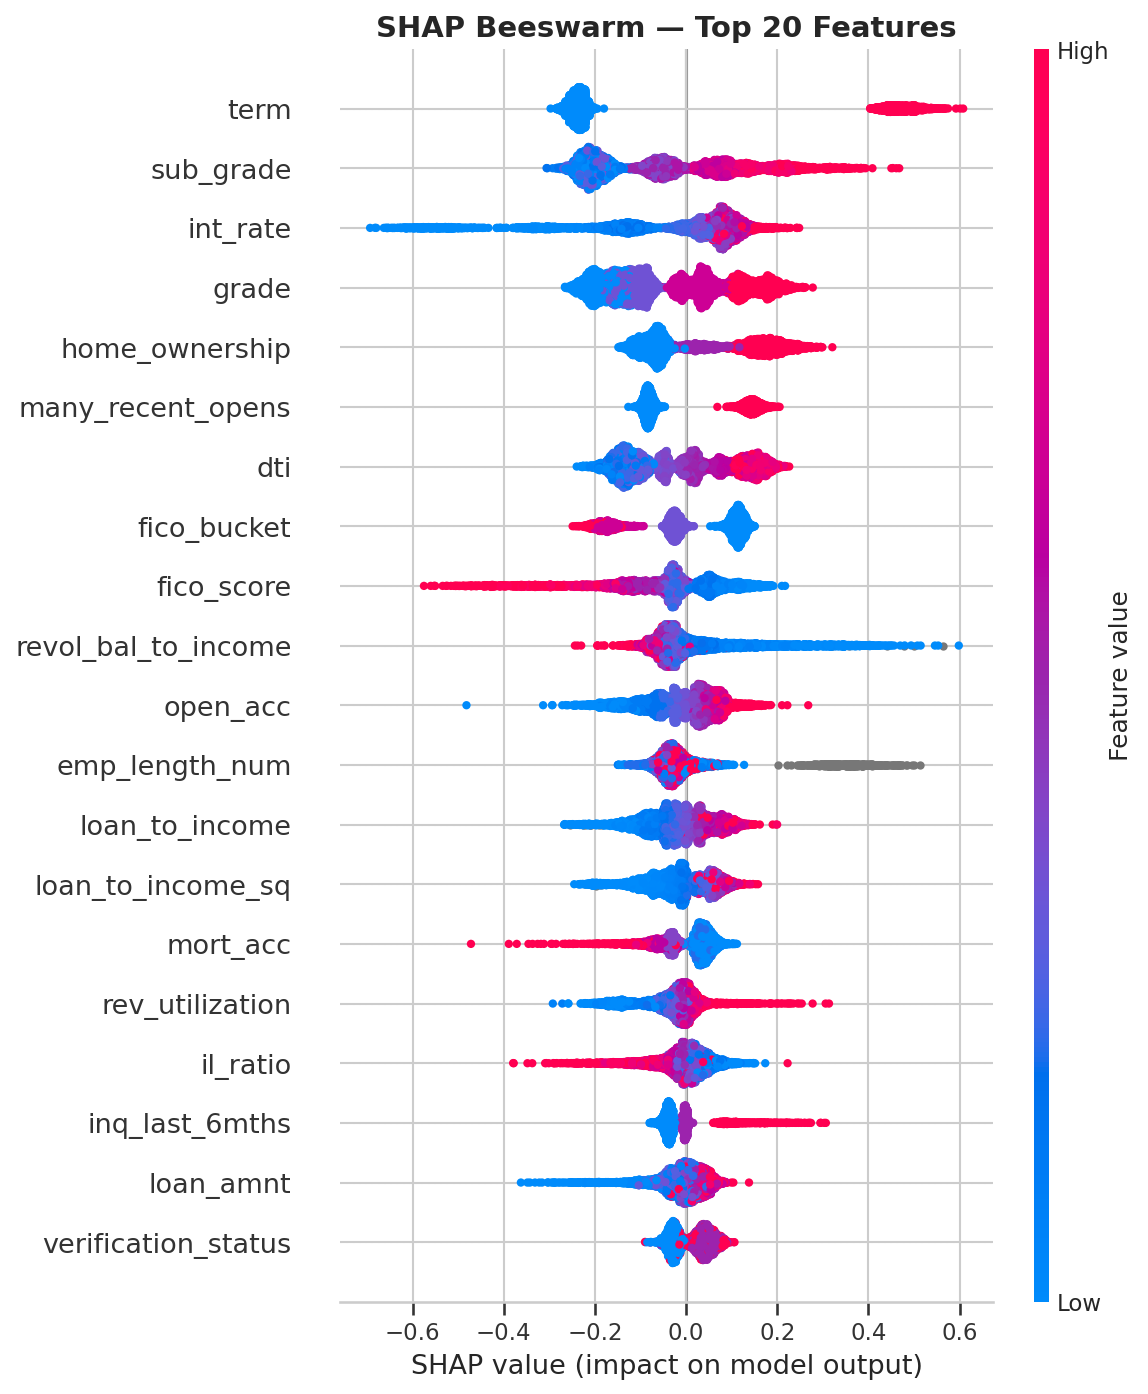
\includegraphics[keepaspectratio,alt={Beeswarm SHAP con contribuciones globales de las variables del modelo PD.}]{chapters/11-explainability/../../assets/figures/notebooks/shap_beeswarm.png}}

}

\caption{\label{fig-shap-beeswarm}Resumen global SHAP del modelo
champion, con las variables que más empujan el score de default.}

\end{figure}%

\end{minipage}%
%
\begin{minipage}[t]{0.50\linewidth}

\begin{figure}[H]

\centering{

\pandocbounded{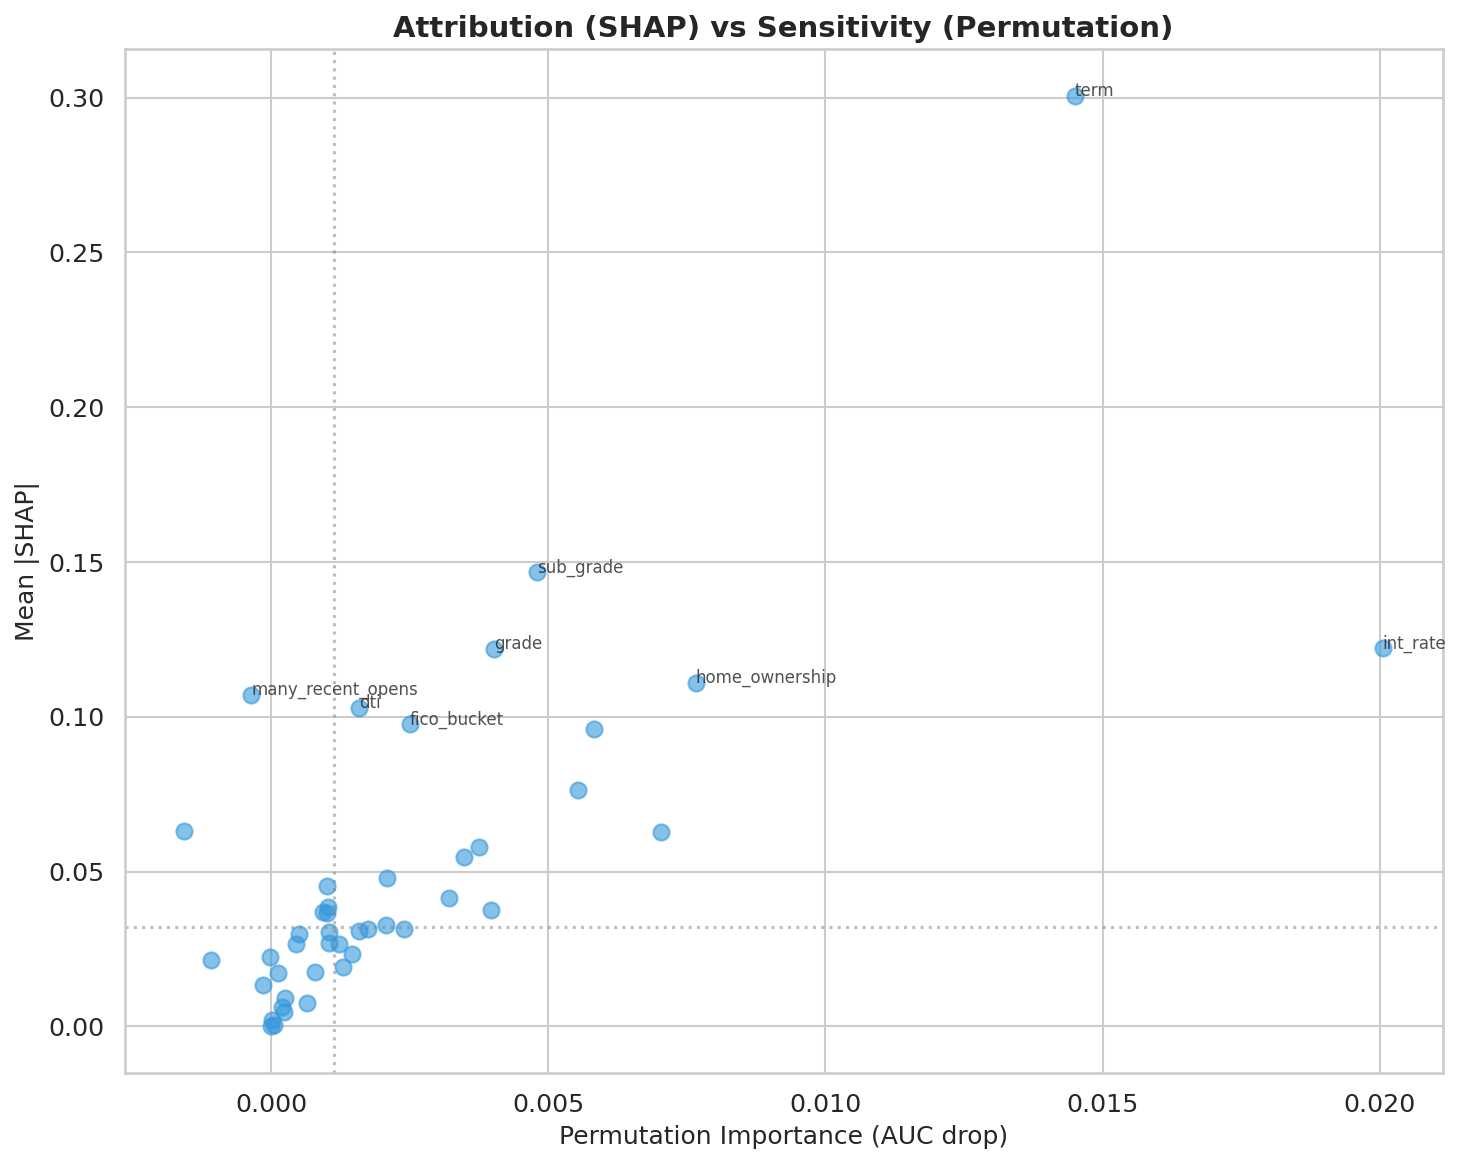
\includegraphics[keepaspectratio,alt={Comparación entre importancia SHAP y permutation importance en el modelo PD.}]{chapters/11-explainability/../../assets/figures/notebooks/shap_vs_permutation.png}}

}

\caption{\label{fig-shap-vs-permutation}Comparación visual entre ranking
SHAP y permutation importance para validar qué señales son
estructurales.}

\end{figure}%

\end{minipage}%

\end{figure*}%

Las figuras Figura~\ref{fig-shap-beeswarm} y
Figura~\ref{fig-shap-vs-permutation} convierten la narrativa global en
evidencia visual: no solo sabemos qué variables aparecen arriba, sino
cómo se distribuye su efecto y qué tan sensible es el desempeño a
perturbarlas.

\subsection{Atribución no es lo mismo que
sensibilidad}\label{atribuciuxf3n-no-es-lo-mismo-que-sensibilidad}

SHAP dice cuánto contribuye una variable al score promedio; permutation
importance dice cuánto cae el AUC si la señal se rompe. Esa distinción
evita sobreinterpretaciones. Por ejemplo:

\begin{longtable}[]{@{}lrr@{}}
\caption{Atribución vs
sensibilidad}\label{tbl-global-vs-permutation}\tabularnewline
\toprule\noalign{}
Variable & \textbar SHAP\textbar{} medio & \texttt{auc\_drop} por
permutación \\
\midrule\noalign{}
\endfirsthead
\toprule\noalign{}
Variable & \textbar SHAP\textbar{} medio & \texttt{auc\_drop} por
permutación \\
\midrule\noalign{}
\endhead
\bottomrule\noalign{}
\endlastfoot
\texttt{int\_rate} & 0.4066 & 0.0754 \\
\texttt{term} & 0.2921 & 0.0144 \\
\texttt{home\_ownership} & 0.1155 & 0.0096 \\
\texttt{fico\_score} & 0.2262 & 0.0088 \\
\end{longtable}

\texttt{int\_rate} domina en ambas métricas, lo que la convierte en el
driver más robusto del sistema. \texttt{term}, en cambio, tiene una
atribución alta pero una sensibilidad menor: empuja muchas predicciones,
aunque el desempeño agregado no colapsa si se degrada parcialmente.

\begin{tcolorbox}[enhanced jigsaw, arc=.35mm, bottomrule=.15mm, bottomtitle=1mm, breakable, colback=white, colbacktitle=quarto-callout-note-color!10!white, colframe=quarto-callout-note-color-frame, coltitle=black, left=2mm, leftrule=.75mm, opacityback=0, opacitybacktitle=0.6, rightrule=.15mm, title=\textcolor{quarto-callout-note-color}{\faInfo}\hspace{0.5em}{Regla de lectura}, titlerule=0mm, toprule=.15mm, toptitle=1mm]

Cuando una variable es alta en SHAP y alta en permutación, suele ser una
señal estructural. Cuando es alta en SHAP pero moderada en permutación,
puede estar capturando contexto frecuente más que dependencia crítica
del modelo.

\end{tcolorbox}

\subsection{Forma funcional con ALE}\label{forma-funcional-con-ale}

Las curvas ALE (\texttt{ale\_curves.parquet}) son la verificación de
monotonía y estabilidad que complementa SHAP. Para \texttt{int\_rate},
el efecto local acumulado pasa de negativo a positivo alrededor del
rango 11-12\%, consistente con una lectura económica razonable: tasas
bajas suelen asociarse a prestatarios más seguros y tasas altas a mayor
riesgo esperado.

La ventaja de ALE frente a PDP es que reduce la distorsión por
correlación entre variables. En un problema crediticio donde
\texttt{int\_rate}, \texttt{fico\_score} y \texttt{grade} están ligados,
esa precaución no es opcional.

\begin{figure*}

\begin{minipage}[t]{0.50\linewidth}

\begin{figure}[H]

\centering{

\pandocbounded{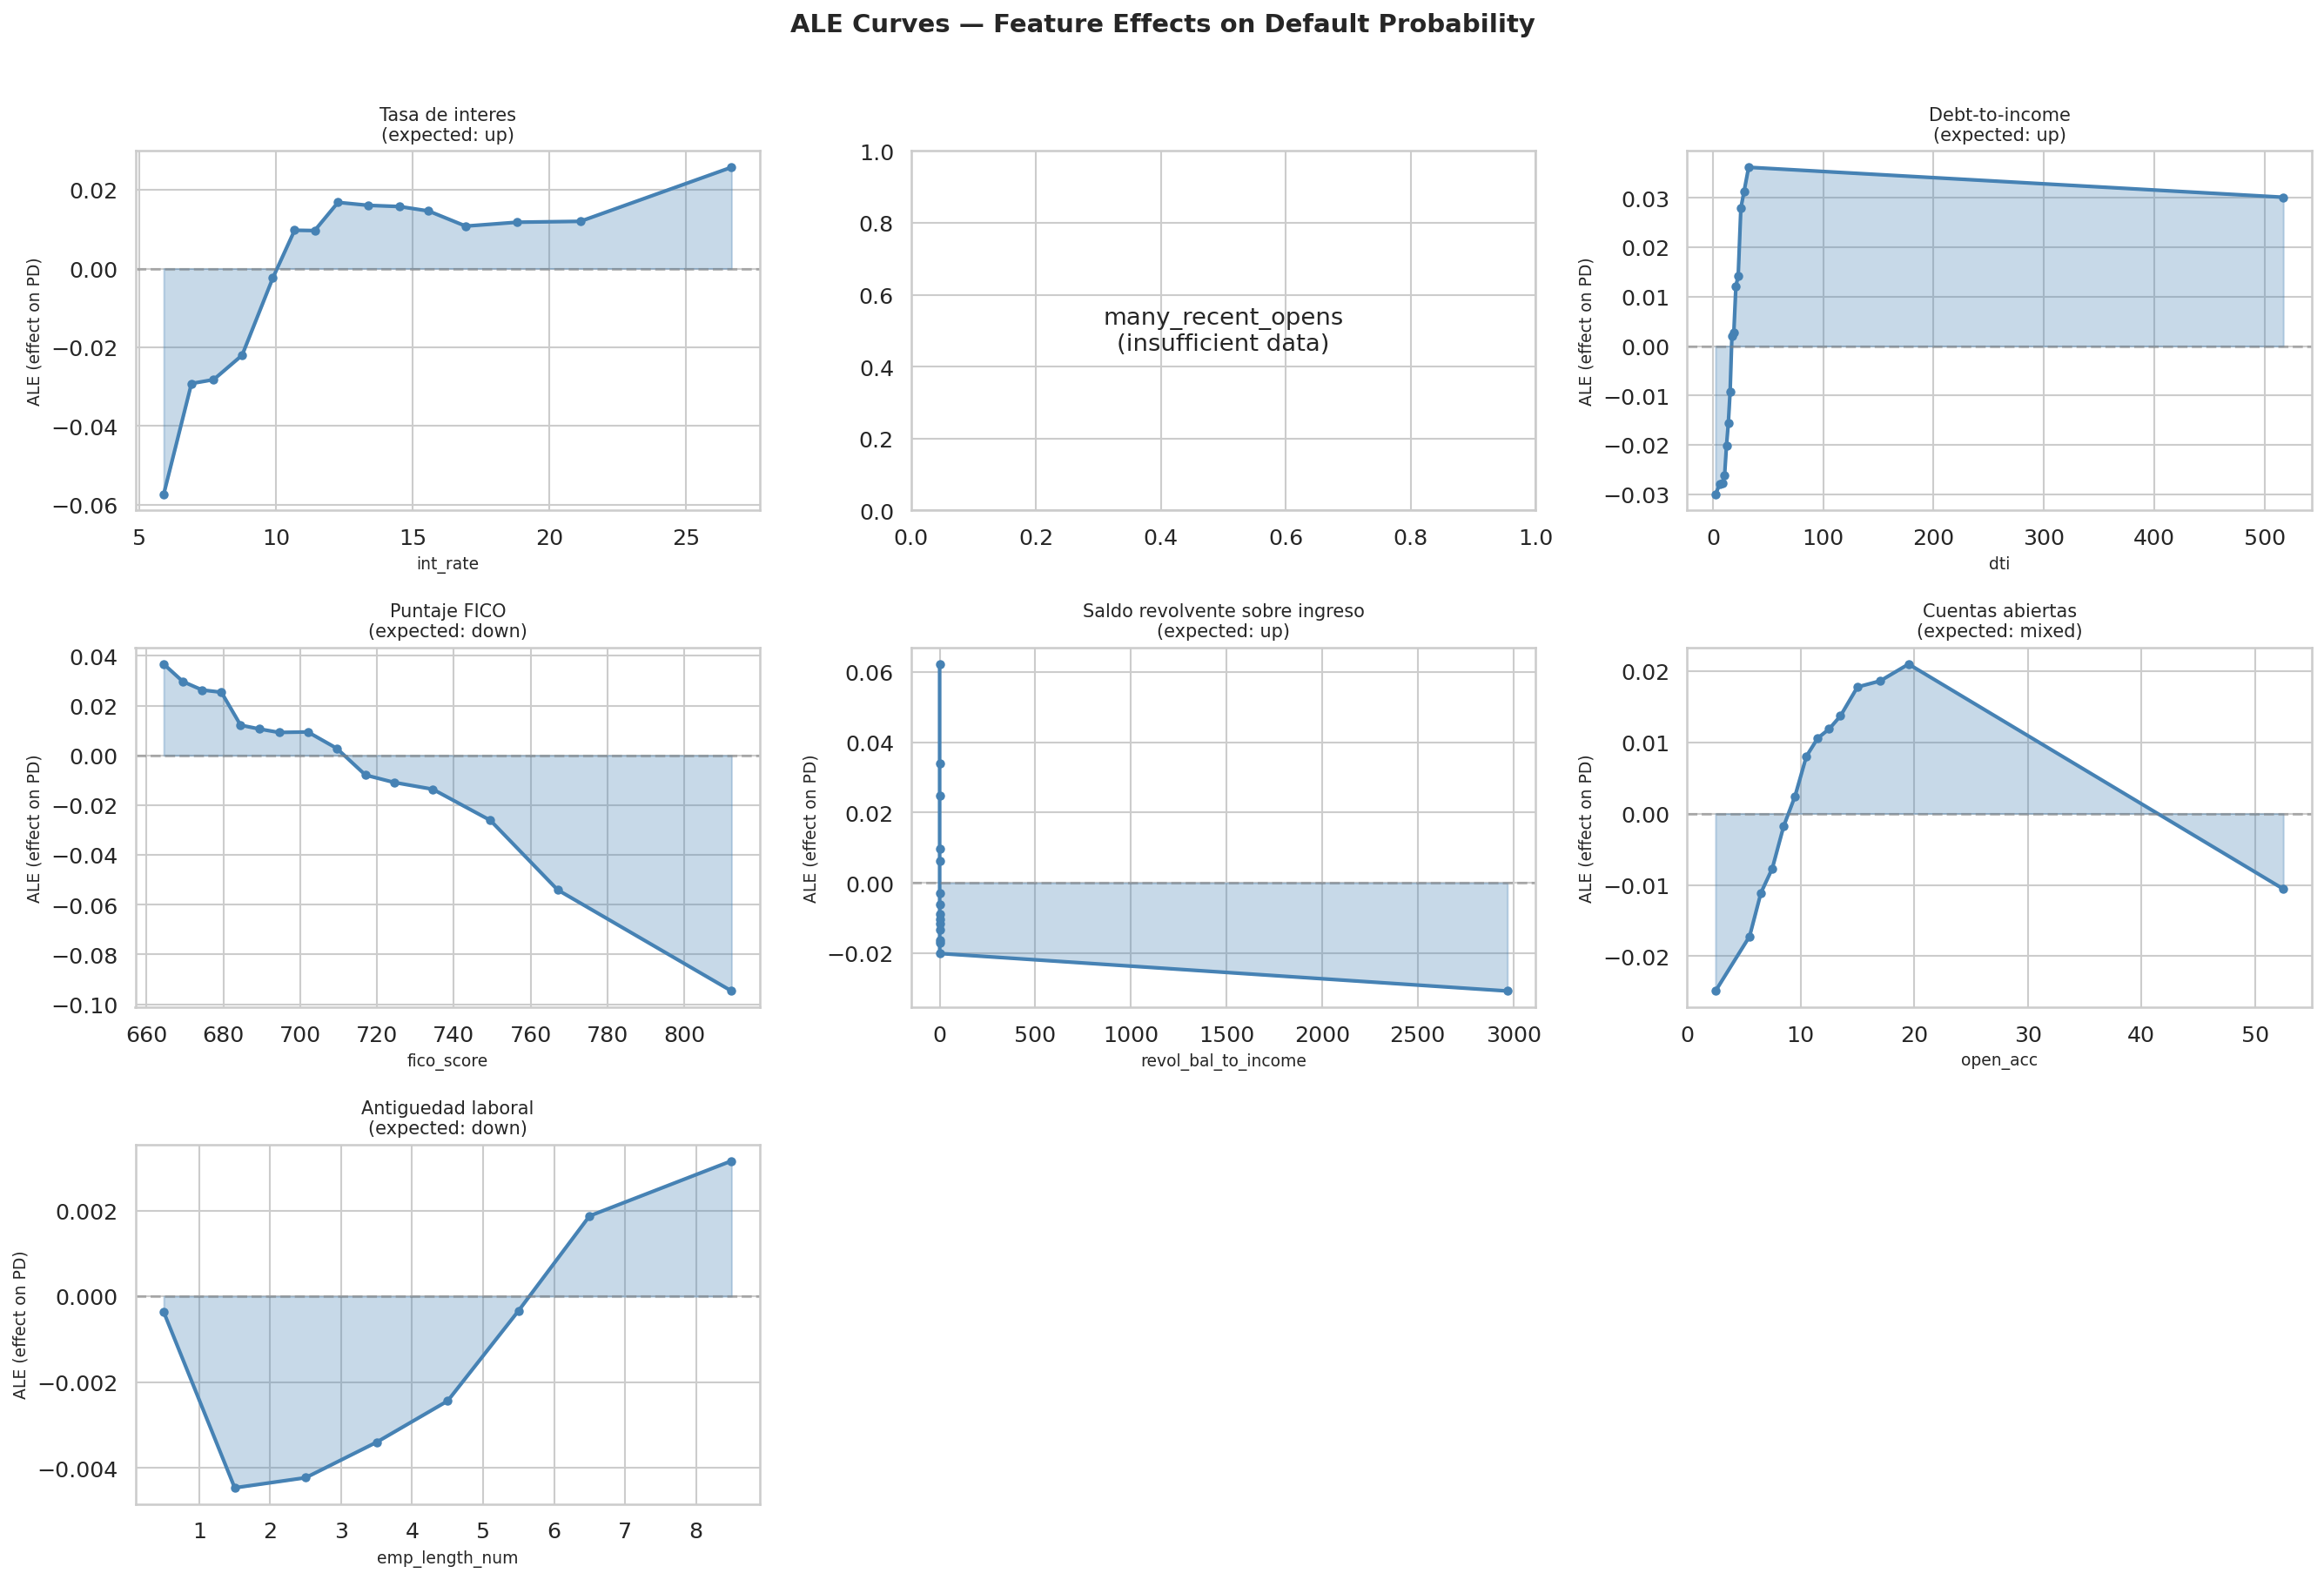
\includegraphics[keepaspectratio,alt={Curvas ALE para variables principales del modelo PD.}]{chapters/11-explainability/../../assets/figures/notebooks/ale_curves.png}}

}

\caption{\label{fig-ale-curves}Curvas ALE de las variables principales,
usadas para verificar forma funcional y monotonías.}

\end{figure}%

\end{minipage}%
%
\begin{minipage}[t]{0.50\linewidth}

\begin{figure}[H]

\centering{

\pandocbounded{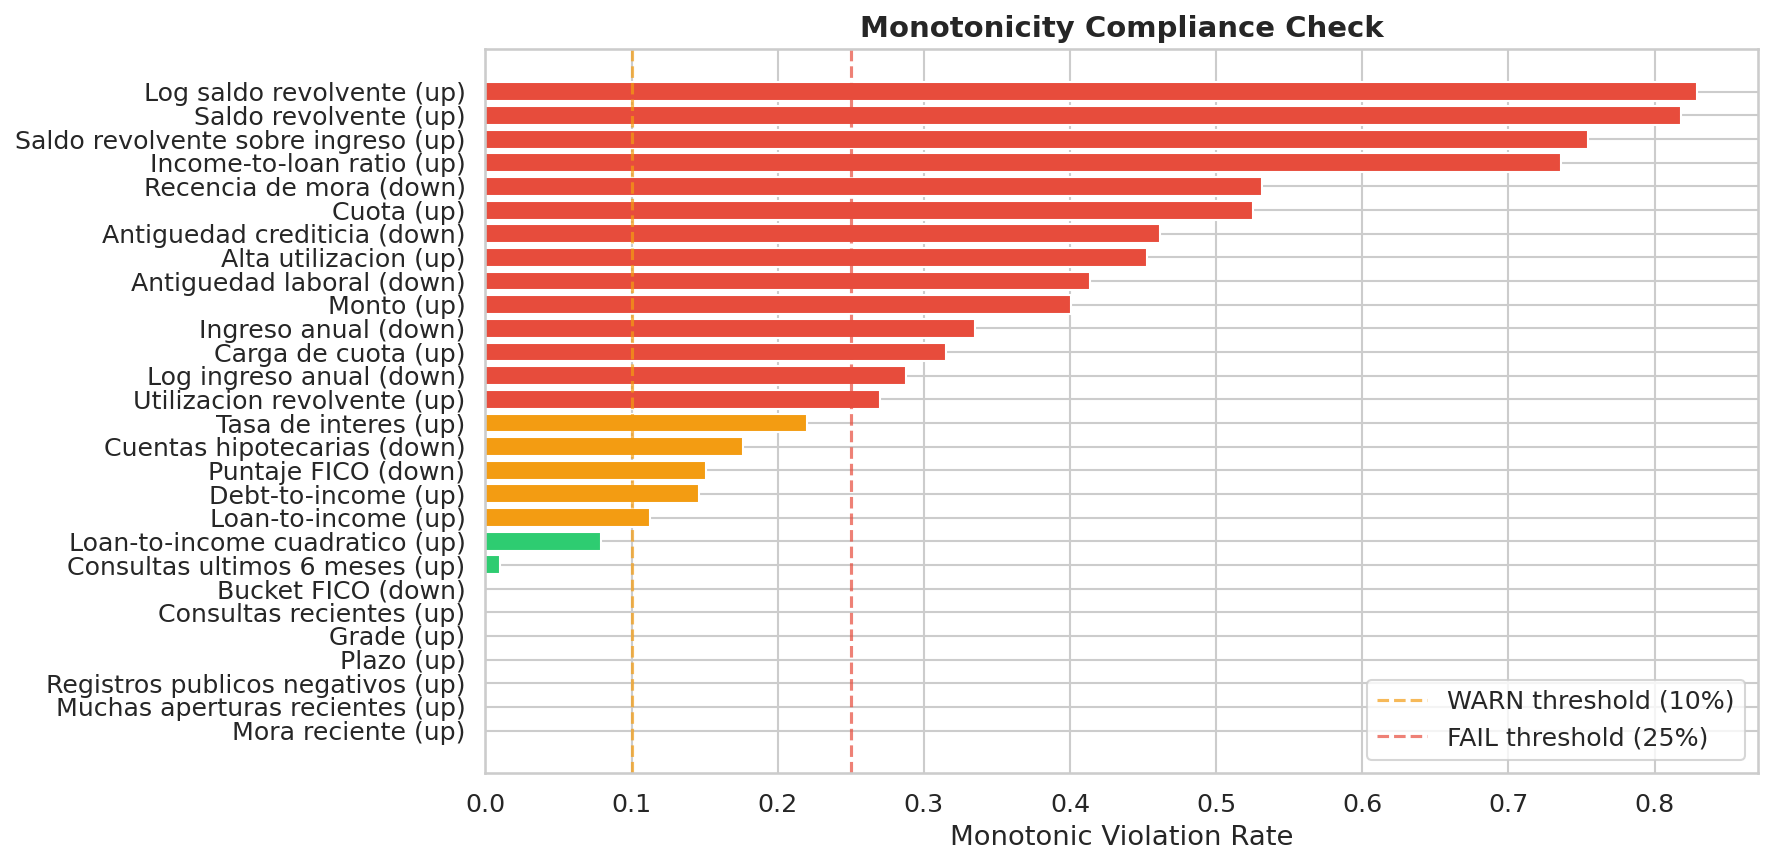
\includegraphics[keepaspectratio,alt={Verificación de monotonía en variables clave del modelo de riesgo.}]{chapters/11-explainability/../../assets/figures/notebooks/monotonicity_verification.png}}

}

\caption{\label{fig-monotonicity-verification}Chequeo de monotonía y
consistencia funcional en variables clave del modelo.}

\end{figure}%

\end{minipage}%

\end{figure*}%

\subsection{Familias de variables y
controlabilidad}\label{familias-de-variables-y-controlabilidad}

El resumen global también clasifica cada feature por familia y
controlabilidad:

\begin{itemize}
\tightlist
\item
  \texttt{pricing}: variables de precio y contrato que pueden
  modificarse por política.
\item
  \texttt{credit\_quality}: señales históricas del prestatario, no
  controlables por originación.
\item
  \texttt{capacity}: capacidad financiera y carga de deuda.
\item
  \texttt{household\_profile}: contexto del hogar y estabilidad.
\end{itemize}

Esta taxonomía permite separar dos conversaciones distintas:

\begin{enumerate}
\def\labelenumi{\arabic{enumi}.}
\tightlist
\item
  qué explica el modelo;
\item
  qué puede ajustar el negocio para mover el riesgo observado.
\end{enumerate}

\begin{figure*}

\begin{minipage}[t]{0.50\linewidth}

\begin{figure}[H]

\centering{

\pandocbounded{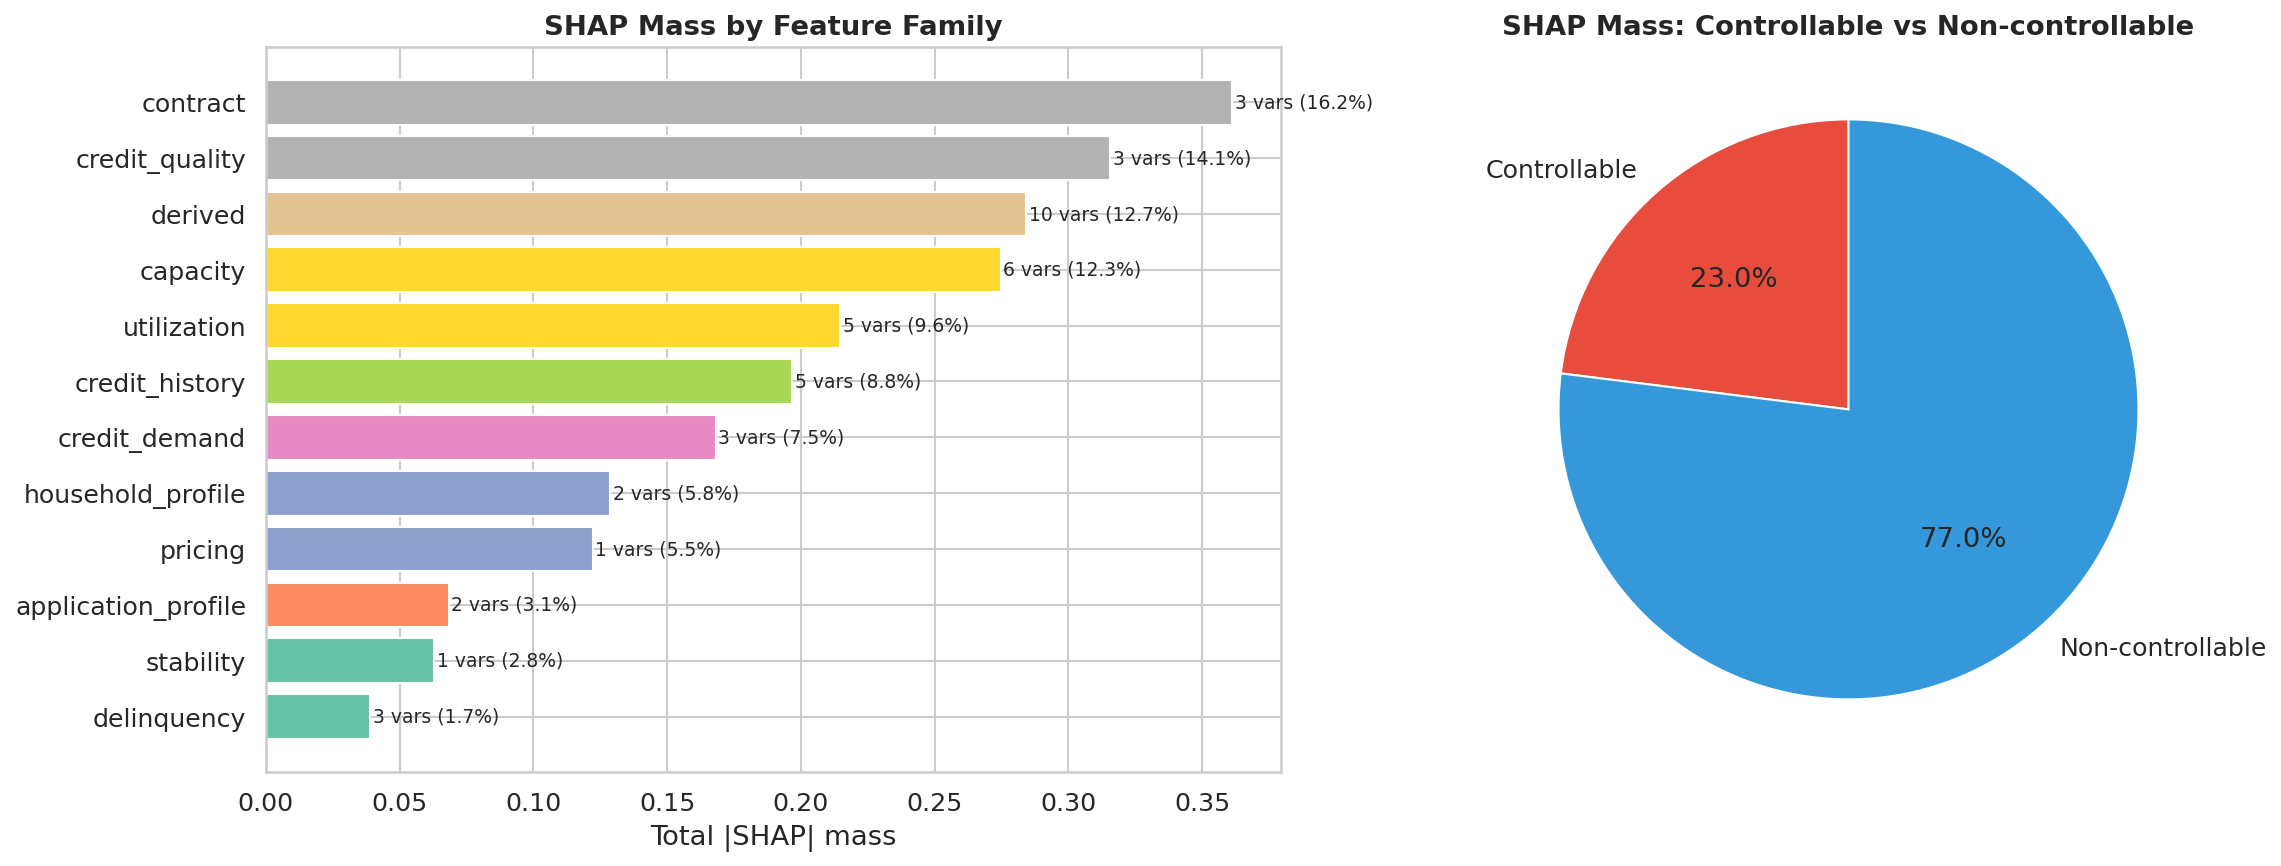
\includegraphics[keepaspectratio,alt={Descomposición de importancia por familias de variables del modelo.}]{chapters/11-explainability/../../assets/figures/notebooks/feature_family_decomposition.png}}

}

\caption{\label{fig-feature-family-decomposition}Descomposición por
familias de variables en las explicaciones globales del modelo.}

\end{figure}%

\end{minipage}%
%
\begin{minipage}[t]{0.50\linewidth}

\begin{figure}[H]

\centering{

\pandocbounded{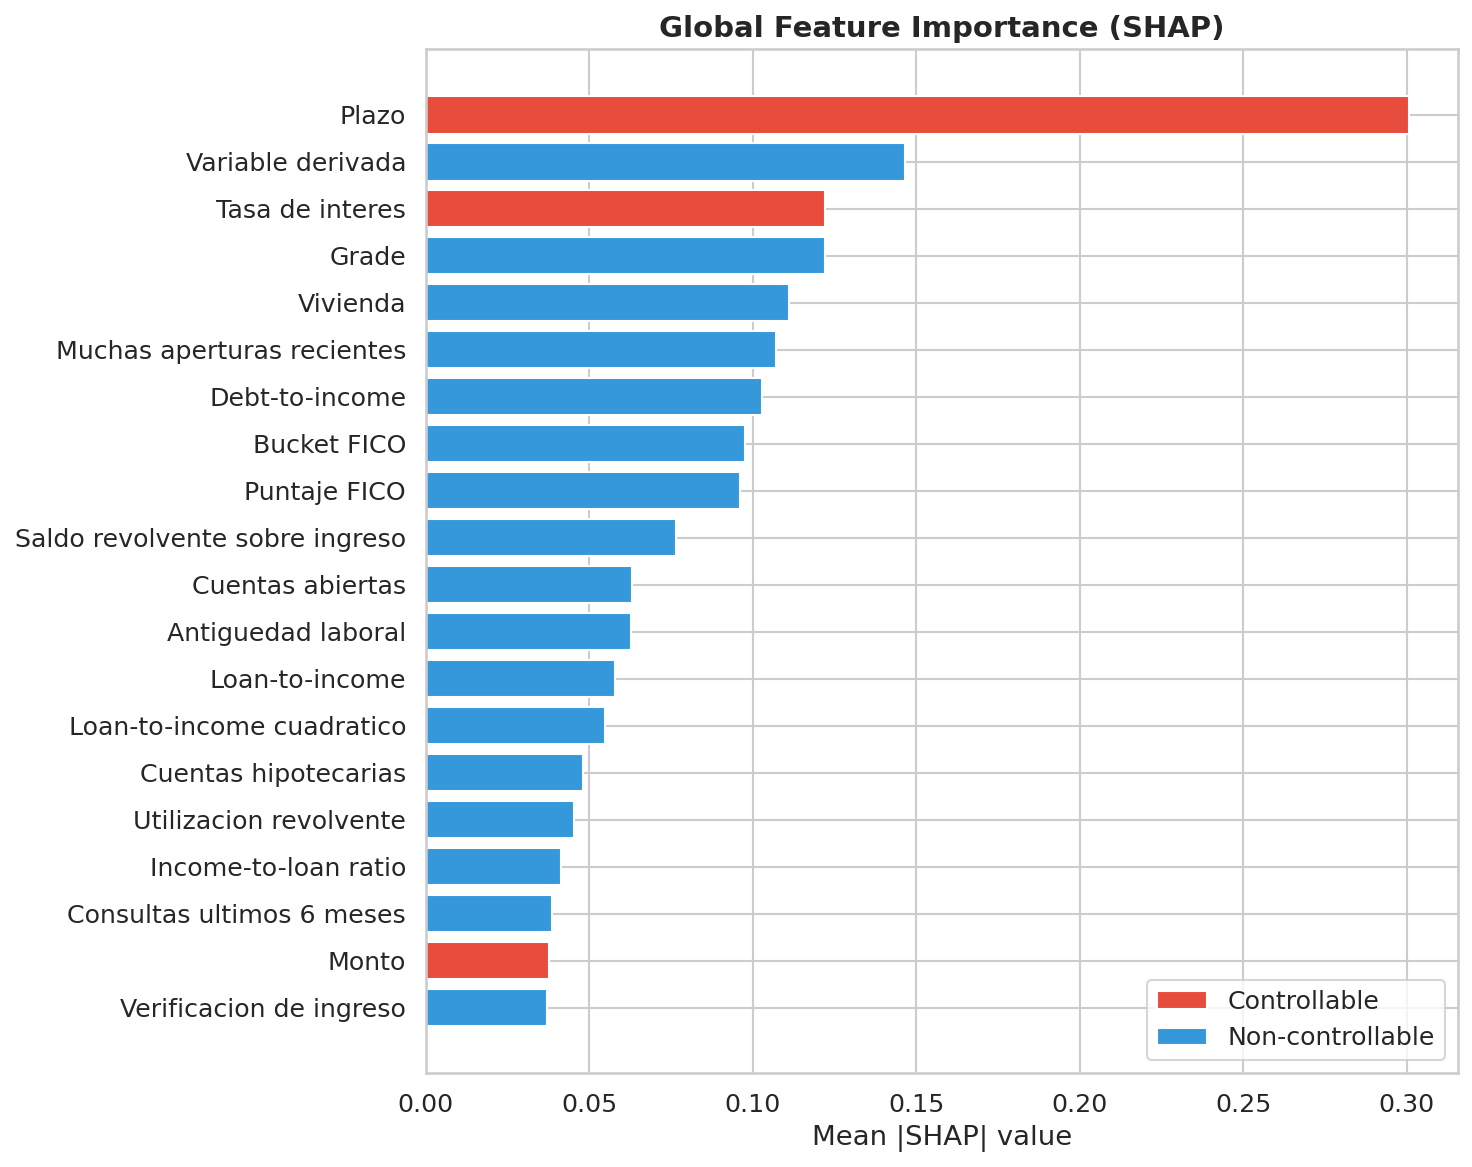
\includegraphics[keepaspectratio,alt={Importancia SHAP global en gráfico de barras.}]{chapters/11-explainability/../../assets/figures/notebooks/shap_bar_importance.png}}

}

\caption{\label{fig-shap-bar}Importancia SHAP agregada en formato barra
para lectura ejecutiva.}

\end{figure}%

\end{minipage}%

\end{figure*}%

En particular, \texttt{int\_rate} y \texttt{term} aparecen como
variables controlables. Eso es útil para pricing y diseño de oferta,
pero exige vigilancia para no caer en una retroalimentación circular
entre precio, selección y riesgo.

\subsection{Apertura metodológica
defendible}\label{apertura-metodoluxf3gica-defendible}

La lección principal de este capítulo es que el modelo sí puede
defenderse globalmente:

\begin{itemize}
\tightlist
\item
  usa drivers económicamente plausibles;
\item
  muestra coherencia entre atribución y sensibilidad;
\item
  conserva monotonías esperadas en variables críticas;
\item
  ofrece una base estable para reason codes locales y monitoreo de
  drift.
\end{itemize}

El siguiente paso es bajar de esta vista de portafolio a casos
concretos, donde la pregunta deja de ser ``qué mueve al modelo en
promedio'' y pasa a ser ``por qué este préstamo quedó donde quedó''.

\chapter{Explicaciones Locales}\label{sec-local-explanations}

Las explicaciones locales convierten una predicción en una decisión
discutible y trazable. Para originación, challenger review y atención a
auditoría, la pregunta no es solo cuánto riesgo tiene un préstamo, sino
\textbf{qué razones concretas empujaron esa evaluación}.

\subsection{Casos representativos
disponibles}\label{casos-representativos-disponibles}

El artefacto \texttt{shap\_local\_cases.parquet} contiene 60 filas que
describen préstamos representativos en distintos segmentos. Cada
registro incluye:

\begin{itemize}
\tightlist
\item
  \texttt{grade} e \texttt{issue\_quarter} para contexto temporal;
\item
  PD puntual y bandas conformales al 90\% y 95\%;
\item
  razones positivas y negativas a nivel de feature;
\item
  familia de feature y marca de controlabilidad.
\end{itemize}

Un caso de bajo riesgo del cuarto trimestre de 2019 ilustra bien el
enfoque:

\begin{longtable}[]{@{}ll@{}}
\caption{Ejemplo de explicación local
defendible}\label{tbl-local-example}\tabularnewline
\toprule\noalign{}
Campo & Valor \\
\midrule\noalign{}
\endfirsthead
\toprule\noalign{}
Campo & Valor \\
\midrule\noalign{}
\endhead
\bottomrule\noalign{}
\endlastfoot
Segmento & \texttt{bajo\_riesgo} \\
Grade & \texttt{A} \\
PD calibrada & 5.64\% \\
Intervalo 90\% & {[}0.00\%, 18.14\%{]} \\
Principales razones a favor & FICO alto, tasa baja, plazo 36 meses \\
\end{longtable}

En este préstamo, el FICO de 767 y la tasa de 8.19\% empujan fuertemente
el score hacia abajo. El resultado es intuitivo para negocio y
consistente con la lectura global del capítulo anterior.

\subsection{Del SHAP a reason codes
operativos}\label{del-shap-a-reason-codes-operativos}

Una explicación local útil debe poder traducirse a reason codes. En este
proyecto, la lógica narrativa se apoya en cuatro familias recurrentes:

\begin{longtable}[]{@{}
  >{\raggedright\arraybackslash}p{(\linewidth - 2\tabcolsep) * \real{0.5000}}
  >{\raggedright\arraybackslash}p{(\linewidth - 2\tabcolsep) * \real{0.5000}}@{}}
\caption{Familias de reason
codes}\label{tbl-reason-families}\tabularnewline
\toprule\noalign{}
\begin{minipage}[b]{\linewidth}\raggedright
Familia
\end{minipage} & \begin{minipage}[b]{\linewidth}\raggedright
Cómo se comunica
\end{minipage} \\
\midrule\noalign{}
\endfirsthead
\toprule\noalign{}
\begin{minipage}[b]{\linewidth}\raggedright
Familia
\end{minipage} & \begin{minipage}[b]{\linewidth}\raggedright
Cómo se comunica
\end{minipage} \\
\midrule\noalign{}
\endhead
\bottomrule\noalign{}
\endlastfoot
\texttt{credit\_quality} & historial y calidad crediticia del
solicitante \\
\texttt{capacity} & presión financiera o capacidad de pago \\
\texttt{pricing} & condiciones del contrato ofrecido \\
\texttt{household\_profile} & estabilidad del hogar y contexto del
solicitante \\
\end{longtable}

La ventaja de esta capa es doble. Primero, evita exponer al usuario
final una lista cruda de variables. Segundo, mantiene consistencia entre
la narrativa de comité y la evidencia técnica subyacente.

\subsection{Qué hace que una explicación local sea
utilizable}\label{quuxe9-hace-que-una-explicaciuxf3n-local-sea-utilizable}

En el contexto de riesgo crediticio, una explicación local útil debe
cumplir al menos tres criterios:

\begin{enumerate}
\def\labelenumi{\arabic{enumi}.}
\tightlist
\item
  ser coherente con la explicación global;
\item
  distinguir señales controlables de señales meramente descriptivas;
\item
  convivir con la banda de incertidumbre, no solo con la predicción
  puntual.
\end{enumerate}

Ese tercer punto es central. Dos préstamos con la misma PD puntual
pueden requerir tratamientos distintos si uno tiene un intervalo mucho
más ancho que el otro. La explicación local no debe ocultar esa
diferencia.

\subsection{Uso en revisión de casos}\label{uso-en-revisiuxf3n-de-casos}

Las explicaciones locales sirven para tres momentos operativos:

\begin{longtable}[]{@{}
  >{\raggedright\arraybackslash}p{(\linewidth - 4\tabcolsep) * \real{0.3333}}
  >{\raggedright\arraybackslash}p{(\linewidth - 4\tabcolsep) * \real{0.3333}}
  >{\raggedright\arraybackslash}p{(\linewidth - 4\tabcolsep) * \real{0.3333}}@{}}
\caption{Usos operativos de explicaciones
locales}\label{tbl-local-uses}\tabularnewline
\toprule\noalign{}
\begin{minipage}[b]{\linewidth}\raggedright
Momento
\end{minipage} & \begin{minipage}[b]{\linewidth}\raggedright
Pregunta de negocio
\end{minipage} & \begin{minipage}[b]{\linewidth}\raggedright
Uso de la explicación
\end{minipage} \\
\midrule\noalign{}
\endfirsthead
\toprule\noalign{}
\begin{minipage}[b]{\linewidth}\raggedright
Momento
\end{minipage} & \begin{minipage}[b]{\linewidth}\raggedright
Pregunta de negocio
\end{minipage} & \begin{minipage}[b]{\linewidth}\raggedright
Uso de la explicación
\end{minipage} \\
\midrule\noalign{}
\endhead
\bottomrule\noalign{}
\endlastfoot
Originación & ¿por qué este préstamo quedó en zona gris? & identificar
palancas de precio, plazo o documentación \\
Validación & ¿la razón local coincide con la teoría del modelo? &
detectar atajos o señales no plausibles \\
Auditoría & ¿puedo reconstruir la decisión? & asociar score, intervalo y
drivers a un caso concreto \\
\end{longtable}

\subsection{Limitaciones}\label{limitaciones}

Las explicaciones locales no prueban causalidad. Describen cómo el
modelo usó la información disponible, no qué cambiaría realmente el
outcome del prestatario en el mundo real. Por eso este libro mantiene
separadas las capas de interpretabilidad y la capa de inferencia causal.

También hay que evitar una falsa sensación de precisión: un \emph{reason
code} es más convincente cuando aparece junto a su contexto de
incertidumbre. En este proyecto, la práctica recomendada es presentar
siempre el trío:

\begin{enumerate}
\def\labelenumi{\arabic{enumi}.}
\tightlist
\item
  PD calibrada,
\item
  intervalo conformal,
\item
  top drivers locales.
\end{enumerate}

Con esa convención, la explicación deja de ser una nota anecdótica y se
convierte en un artefacto formal de decisión.

\chapter{Drift de Explicaciones}\label{sec-explanation-drift}

La estabilidad de un modelo no se evalúa solo por AUC o cobertura. Un
sistema puede conservar desempeño aceptable mientras cambia
silenciosamente la narrativa de por qué decide. Ese riesgo es
especialmente sensible en crédito, donde comités y validadores esperan
continuidad económica en los drivers.

\subsection{Qué se monitorea}\label{quuxe9-se-monitorea}

El artefacto \texttt{explanation\_drift.parquet} compara un periodo de
referencia amplio (\texttt{2018Q1}-\texttt{2019Q3}) con un periodo de
contraste (\texttt{2019Q4}-\texttt{2020Q3}). La evaluación resume tres
preguntas:

\begin{enumerate}
\def\labelenumi{\arabic{enumi}.}
\tightlist
\item
  ¿se conservan los top drivers globales?
\item
  ¿cambió materialmente la distribución SHAP de los drivers críticos?
\item
  ¿los reason codes dominantes siguen contando la misma historia?
\end{enumerate}

\subsection{Resultado del snapshot
actual}\label{resultado-del-snapshot-actual}

\begin{longtable}[]{@{}lrl@{}}
\caption{Resumen de drift
explicativo}\label{tbl-explanation-drift}\tabularnewline
\toprule\noalign{}
Indicador & Valor & Lectura \\
\midrule\noalign{}
\endfirsthead
\toprule\noalign{}
Indicador & Valor & Lectura \\
\midrule\noalign{}
\endhead
\bottomrule\noalign{}
\endlastfoot
\texttt{rank\_overlap\_top10} & 1.00 & mismo top 10 global \\
\texttt{avg\_shap\_psi\_top5} & 0.0491 & cambio pequeño en masa SHAP \\
\texttt{max\_shap\_psi\_top5} & 0.0757 & sin desplazamiento severo \\
\texttt{reason\_code\_match\_rate} & 1.00 & reason codes líderes
estables \\
\texttt{passed\_all} & \texttt{True} & snapshot en verde \\
\end{longtable}

Los detalles internos muestran que \texttt{int\_rate}, \texttt{term},
\texttt{fico\_score}, \texttt{dti} y \texttt{home\_ownership} siguen
siendo el corazón del modelo. Ese resultado es valioso porque el periodo
de comparación incluye un entorno de mercado más exigente.

\subsection{Por qué esto importa para
gobernanza}\label{por-quuxe9-esto-importa-para-gobernanza}

Si el ranking de drivers cambia abruptamente, aparecen dos hipótesis
incómodas:

\begin{itemize}
\tightlist
\item
  el modelo empezó a explotar una señal espuria;
\item
  el proceso de datos cambió y ya no estamos midiendo el mismo fenómeno.
\end{itemize}

El drift explicativo funciona entonces como una alarma temprana entre el
monitoreo de datos y el monitoreo de performance. No sustituye PSI, KS o
cobertura conformal, pero complementa esos controles con una capa
semántica.

\begin{tcolorbox}[enhanced jigsaw, arc=.35mm, bottomrule=.15mm, bottomtitle=1mm, breakable, colback=white, colbacktitle=quarto-callout-tip-color!10!white, colframe=quarto-callout-tip-color-frame, coltitle=black, left=2mm, leftrule=.75mm, opacityback=0, opacitybacktitle=0.6, rightrule=.15mm, title=\textcolor{quarto-callout-tip-color}{\faLightbulb}\hspace{0.5em}{Señal de confianza}, titlerule=0mm, toprule=.15mm, toptitle=1mm]

Un \texttt{rank\_overlap\_top10\ =\ 1.00} no significa ``inmutabilidad
total''; significa que la narrativa económica principal del modelo
sobrevivió al cambio de periodo. Eso aumenta la defendibilidad del
sistema frente a revisores humanos.

\end{tcolorbox}

\subsection{Relación con drift de
datos}\label{relaciuxf3n-con-drift-de-datos}

El capítulo de monitoreo de datos ya mostró que varias variables
experimentan desplazamientos detectables por KS o CvM. El punto
interesante es que esos movimientos no se tradujeron, por ahora, en una
ruptura del mapa explicativo central. En otras palabras:

\[
\text{data drift} \not\Rightarrow \text{explanation drift severo}
\]

Esta separación permite respuestas más finas. No toda alerta de datos
requiere reentrenamiento inmediato; algunas pueden manejarse con
observación reforzada si la lógica explicativa y la cobertura siguen
siendo estables.

\subsection{Limitaciones}\label{limitaciones-1}

El snapshot actual es corto y agregado. Todavía falta:

\begin{enumerate}
\def\labelenumi{\arabic{enumi}.}
\tightlist
\item
  ampliar la comparación por segmento y por grade;
\item
  medir estabilidad trimestral continua, no solo dos ventanas agregadas;
\item
  vincular alertas explicativas con reglas automáticas de escalamiento
  en MRM.
\end{enumerate}

Pese a ello, el estado actual ya mejora mucho la práctica usual: el
proyecto no solo reporta qué tan bien predice el modelo, sino si sigue
contando la misma historia económica a lo largo del tiempo.

\chapter{Dataset 360°}\label{dataset-360}

Una visión completa del dataset de Lending Club como plataforma de
investigación: desde el análisis exploratorio hasta el benchmarking
contra la literatura publicada.

\chapter{Hallazgos Clave del EDA}\label{sec-eda-highlights}

El EDA del proyecto no es una introducción decorativa; fija el contrato
de realidad sobre el que descansan todos los capítulos posteriores.
Antes de modelar, conviene dejar congelados tres hechos: el tamaño del
universo, la tasa de default y el gradiente económico del riesgo.

\subsection{Universo analítico}\label{universo-analuxedtico}

En el split de entrenamiento usado para construcción de features y
modelado principal, el artefacto \texttt{eda\_summary.json} reporta:

\begin{longtable}[]{@{}lr@{}}
\caption{Radiografía del dataset de
entrenamiento}\label{tbl-eda-core}\tabularnewline
\toprule\noalign{}
Indicador & Valor \\
\midrule\noalign{}
\endfirsthead
\toprule\noalign{}
Indicador & Valor \\
\midrule\noalign{}
\endhead
\bottomrule\noalign{}
\endlastfoot
Préstamos analizados & 1,346,311 \\
Tasa global de default & 18.52\% \\
Registros con plazo 36m & 1,005,656 \\
Registros con plazo 60m & 340,655 \\
\end{longtable}

La mezcla de plazos confirma que el problema no es homogéneo: una
porción material del portafolio está expuesta a horizontes contractuales
largos, lo que justifica el uso posterior de supervivencia, IFRS9
lifetime y escenarios temporales.

\subsection{Gradiente de riesgo por
grade}\label{gradiente-de-riesgo-por-grade}

La señal más importante del EDA es el orden económico del default por
grade:

\begin{longtable}[]{@{}lr@{}}
\caption{Gradiente de riesgo por
grade}\label{tbl-eda-grade}\tabularnewline
\toprule\noalign{}
Grade & Default rate \\
\midrule\noalign{}
\endfirsthead
\toprule\noalign{}
Grade & Default rate \\
\midrule\noalign{}
\endhead
\bottomrule\noalign{}
\endlastfoot
A & 5.63\% \\
B & 12.29\% \\
C & 20.64\% \\
D & 28.31\% \\
E & 36.47\% \\
F & 43.44\% \\
G & 47.71\% \\
\end{longtable}

Este patrón valida dos decisiones estructurales del libro:

\begin{enumerate}
\def\labelenumi{\arabic{enumi}.}
\tightlist
\item
  usar \texttt{grade} como partición natural para análisis conformales y
  lectura prudencial;
\item
  tratar la tasa de interés y el precio de originación como variables
  centrales de interpretación.
\end{enumerate}

\begin{figure*}

\centering{

\pandocbounded{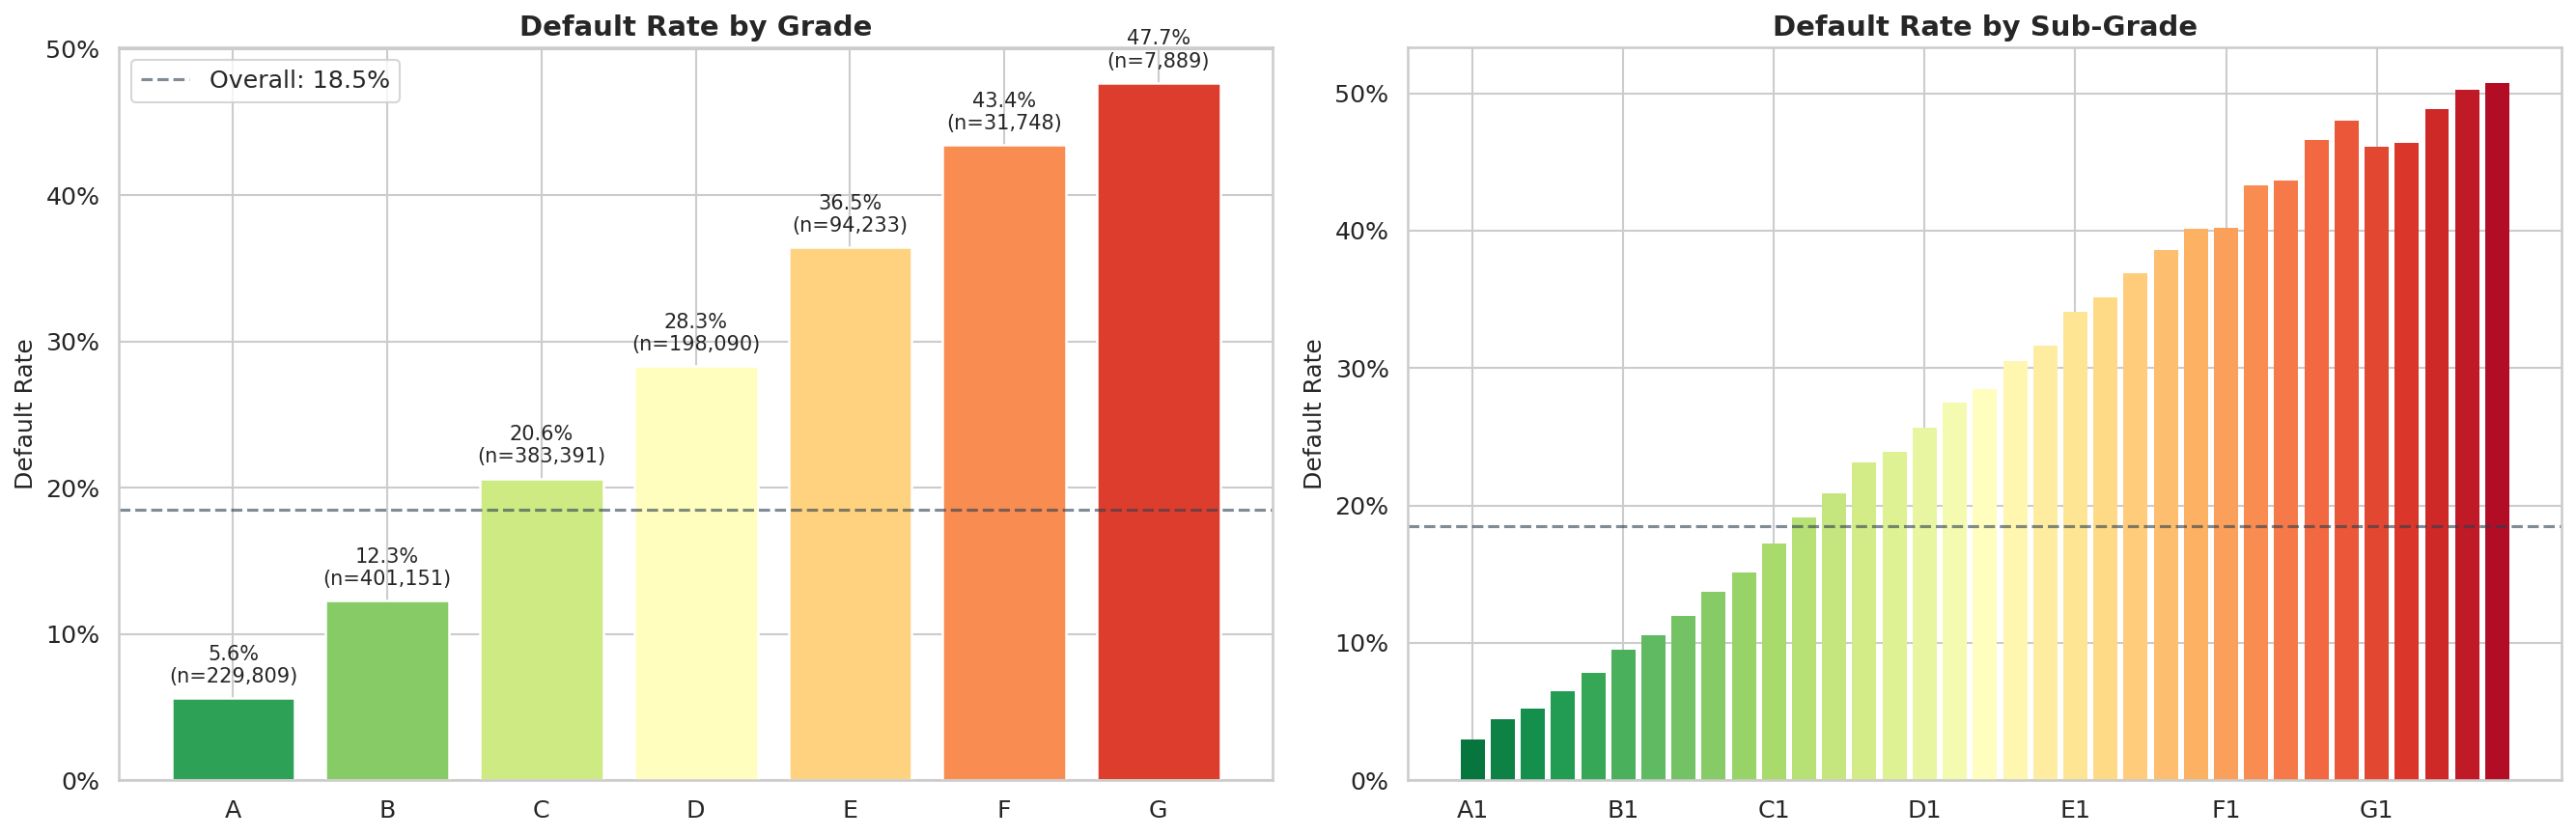
\includegraphics[keepaspectratio,alt={Gráfico de tasa de default por grade desde A hasta G en el dataset Lending Club.}]{chapters/12-dataset-360/../../assets/figures/notebooks/default_rate_by_grade.png}}

}

\caption{\label{fig-default-rate-grade}Tasa de default por grade en
Lending Club, usada como evidencia base del gradiente económico de
riesgo.}

\end{figure*}%

La figura Figura~\ref{fig-default-rate-grade} hace visible el orden
económico que luego reaparece en conformal, IFRS9 y optimización: el
dataset sí tiene una estructura de riesgo interpretable y consistente.

\subsection{Lecturas que sí importan}\label{lecturas-que-suxed-importan}

El EDA deja tres mensajes prácticos:

\begin{itemize}
\tightlist
\item
  el riesgo no está uniformemente distribuido;
\item
  existe una mezcla fuerte de segmentos, no un ``prestatario promedio''
  representativo;
\item
  cualquier validación aleatoria sería demasiado optimista frente a la
  dinámica temporal real.
\end{itemize}

Por eso el pipeline se apoya en \emph{out-of-time validation} y no en
validación IID ingenua.

\subsection{Variables con contenido
económico}\label{variables-con-contenido-econuxf3mico}

Aunque el dataset es amplio, el proyecto organiza la historia en torno a
unas pocas familias con interpretación clara:

\begin{longtable}[]{@{}
  >{\raggedright\arraybackslash}p{(\linewidth - 4\tabcolsep) * \real{0.3333}}
  >{\raggedright\arraybackslash}p{(\linewidth - 4\tabcolsep) * \real{0.3333}}
  >{\raggedright\arraybackslash}p{(\linewidth - 4\tabcolsep) * \real{0.3333}}@{}}
\caption{Familias con valor narrativo y
operativo}\label{tbl-eda-families}\tabularnewline
\toprule\noalign{}
\begin{minipage}[b]{\linewidth}\raggedright
Familia
\end{minipage} & \begin{minipage}[b]{\linewidth}\raggedright
Variables emblemáticas
\end{minipage} & \begin{minipage}[b]{\linewidth}\raggedright
Papel en la narrativa
\end{minipage} \\
\midrule\noalign{}
\endfirsthead
\toprule\noalign{}
\begin{minipage}[b]{\linewidth}\raggedright
Familia
\end{minipage} & \begin{minipage}[b]{\linewidth}\raggedright
Variables emblemáticas
\end{minipage} & \begin{minipage}[b]{\linewidth}\raggedright
Papel en la narrativa
\end{minipage} \\
\midrule\noalign{}
\endhead
\bottomrule\noalign{}
\endlastfoot
Precio / contrato & \texttt{int\_rate}, \texttt{term} & resumen del
riesgo percibido en originación \\
Calidad crediticia & \texttt{fico\_score}, historial & solvencia previa
del cliente \\
Capacidad & \texttt{dti}, ingreso & presión financiera \\
Perfil del hogar & \texttt{home\_ownership}, verificación & estabilidad
y contexto \\
\end{longtable}

\subsection{Qué habilita este
capítulo}\label{quuxe9-habilita-este-capuxedtulo}

Con este diagnóstico, el resto del libro deja de depender de intuiciones
blandas. El EDA justifica:

\begin{itemize}
\tightlist
\item
  la ingeniería de variables posterior;
\item
  la partición temporal train/cal/test;
\item
  la elección de métricas y grupos para fairness, drift y cobertura;
\item
  la lectura prudencial de los resultados IFRS9.
\end{itemize}

El objetivo no es ``mostrar gráficos bonitos'', sino fijar el terreno
sobre el cual una decisión de riesgo puede ser defendida.

\chapter{Análisis Geográfico y Temporal}\label{sec-geographic-temporal}

La heterogeneidad geográfica y temporal es una de las razones por las
que este problema no puede tratarse como una tabla tabular estática. El
mismo score puede significar cosas distintas cuando cambia el estado, el
ciclo crediticio o el régimen macroeconómico.

\subsection{Cobertura geográfica}\label{cobertura-geogruxe1fica}

El artefacto \texttt{state\_aggregates.parquet} resume 51
jurisdicciones. La dispersión es amplia tanto en volumen como en
default:

\begin{longtable}[]{@{}lrrr@{}}
\caption{Muestra del agregado
geográfico}\label{tbl-state-sample}\tabularnewline
\toprule\noalign{}
Estado & N préstamos & Default rate & Volumen total \\
\midrule\noalign{}
\endfirsthead
\toprule\noalign{}
Estado & N préstamos & Default rate & Volumen total \\
\midrule\noalign{}
\endhead
\bottomrule\noalign{}
\endlastfoot
CA & 264,525 & 19.47\% & \$3.94B \\
AZ & 45,521 & 19.03\% & \$0.64B \\
AL & 22,802 & 22.72\% & \$0.32B \\
AR & 14,087 & 23.62\% & \$0.19B \\
AK & 4,343 & 18.97\% & \$0.07B \\
\end{longtable}

La presencia de estados con mucho menor soporte muestral también es una
advertencia metodológica: no toda heterogeneidad observable amerita una
partición operacional. En varios capítulos posteriores se privilegia
\texttt{grade} como grupo Mondrian precisamente porque tiene mejor
estabilidad y sentido regulatorio.

\subsection{No estacionariedad
temporal}\label{no-estacionariedad-temporal}

El proyecto usa una división temporal explícita, no un \emph{shuffle
split}. La narrativa sincronizada con la tesis fija el esquema canónico:

\begin{longtable}[]{@{}lrl@{}}
\caption{Esquema temporal del
pipeline}\label{tbl-temporal-split}\tabularnewline
\toprule\noalign{}
Split & Filas & Periodo narrativo \\
\midrule\noalign{}
\endfirsthead
\toprule\noalign{}
Split & Filas & Periodo narrativo \\
\midrule\noalign{}
\endhead
\bottomrule\noalign{}
\endlastfoot
Train & 1,346,311 & 2007-2017 \\
Calibration & 237,584 & ventana de ajuste intermedia \\
Test OOT & 276,869 & 2018-2020 \\
\end{longtable}

Esta estructura cumple dos objetivos. Primero, evita contaminación entre
desarrollo y evaluación. Segundo, reproduce la forma en que un banco
realmente desplegaría el modelo: entrenando en historia conocida y
enfrentándolo luego a un periodo futuro.

\subsection{La geografía no es solo un
mapa}\label{la-geografuxeda-no-es-solo-un-mapa}

En crédito, el estado resume mezcla de regulación local, composición
sectorial, mercado laboral y comportamiento del prestatario. Sin
embargo, este libro evita sobredimensionar esa dimensión. La lectura
correcta es:

\begin{itemize}
\tightlist
\item
  la geografía aporta contexto;
\item
  el tiempo aporta el verdadero test de robustez;
\item
  la combinación de ambos obliga a monitoreo continuo.
\end{itemize}

\subsection{Por qué la validación temporal
manda}\label{por-quuxe9-la-validaciuxf3n-temporal-manda}

La evidencia de drift en variables como \texttt{fico\_score} e
\texttt{int\_rate} confirma que el portafolio cambia en el tiempo. Si a
eso se suma la heterogeneidad por estado, el costo de ignorar la
dimensión temporal sería alto:

\[
\text{validación aleatoria} \;\Rightarrow\; \text{optimismo artificial en desempeño y cobertura}
\]

Por eso los resultados fuertes del libro se reportan siempre en ventanas
OOT o con trazabilidad temporal explícita.

\subsection{Implicación para capítulos
posteriores}\label{implicaciuxf3n-para-capuxedtulos-posteriores}

Este capítulo habilita tres decisiones de diseño:

\begin{enumerate}
\def\labelenumi{\arabic{enumi}.}
\tightlist
\item
  monitoreo de drift con PSI, KS y CvM;
\item
  cobertura conformal evaluada por cohorte temporal y por grupo;
\item
  escenarios IFRS9 y proyecciones ECL como extensiones naturales del
  análisis temporal.
\end{enumerate}

La conclusión de fondo es sencilla: el dataset no es solo grande; es
dinámico y heterogéneo. El pipeline completo fue construido para
respetar esa realidad.

\chapter{Benchmark contra Literatura}\label{sec-literature-benchmark}

El valor de este libro no depende de superar un leaderboard aislado. Aun
así, es importante ubicar el resultado del pipeline frente a referencias
publicadas para evitar dos errores opuestos: vender de más lo conseguido
o subestimar su relevancia.

\subsection{Punto de comparación
disponible}\label{punto-de-comparaciuxf3n-disponible}

El artefacto \texttt{lendingclub\_literature\_benchmark.parquet}
registra una referencia explícita revisada por pares sobre Lending Club:

\begin{longtable}[]{@{}
  >{\raggedright\arraybackslash}p{(\linewidth - 4\tabcolsep) * \real{0.3000}}
  >{\raggedright\arraybackslash}p{(\linewidth - 4\tabcolsep) * \real{0.3000}}
  >{\raggedleft\arraybackslash}p{(\linewidth - 4\tabcolsep) * \real{0.4000}}@{}}
\caption{Benchmark externo curado para Lending
Club}\label{tbl-literature-benchmark}\tabularnewline
\toprule\noalign{}
\begin{minipage}[b]{\linewidth}\raggedright
Fuente
\end{minipage} & \begin{minipage}[b]{\linewidth}\raggedright
Familia de modelo
\end{minipage} & \begin{minipage}[b]{\linewidth}\raggedleft
AUC reportado
\end{minipage} \\
\midrule\noalign{}
\endfirsthead
\toprule\noalign{}
\begin{minipage}[b]{\linewidth}\raggedright
Fuente
\end{minipage} & \begin{minipage}[b]{\linewidth}\raggedright
Familia de modelo
\end{minipage} & \begin{minipage}[b]{\linewidth}\raggedleft
AUC reportado
\end{minipage} \\
\midrule\noalign{}
\endhead
\bottomrule\noalign{}
\endlastfoot
Li et al.~(2022, benchmark Lending Club) & LightGBM / Gradient Boosting
& 0.7492 \\
Survey de explicabilidad P2P & Árboles + SHAP/LIME & n/a \\
\end{longtable}

Nuestro pipeline canónico reporta \texttt{AUC\ =\ 0.7130} para CatBoost
calibrado con Venn-Abers sobre evaluación OOT.

\subsection{Comparación correcta, no
tramposa}\label{comparaciuxf3n-correcta-no-tramposa}

La diferencia entre 0.7130 y 0.7492 \textbf{no} debe leerse
automáticamente como inferioridad metodológica. Hay al menos tres
razones:

\begin{enumerate}
\def\labelenumi{\arabic{enumi}.}
\tightlist
\item
  el protocolo de split puede no coincidir;
\item
  el objetivo del proyecto no es solo maximizar AUC, sino producir
  probabilidades calibradas y gobernables;
\item
  el libro optimiza un pipeline completo con incertidumbre, IFRS9,
  explicabilidad y robustez, no solo clasificación.
\end{enumerate}

En otras palabras, una comparación honesta requiere comparar tanto el
contexto experimental como el producto final de decisión.

\begin{tcolorbox}[enhanced jigsaw, arc=.35mm, bottomrule=.15mm, bottomtitle=1mm, breakable, colback=white, colbacktitle=quarto-callout-note-color!10!white, colframe=quarto-callout-note-color-frame, coltitle=black, left=2mm, leftrule=.75mm, opacityback=0, opacitybacktitle=0.6, rightrule=.15mm, title=\textcolor{quarto-callout-note-color}{\faInfo}\hspace{0.5em}{Métrica líder vs sistema líder}, titlerule=0mm, toprule=.15mm, toptitle=1mm]

Una AUC más alta puede coexistir con peor calibración, peor cobertura y
menor capacidad de auditoría. Este libro privilegia el sistema líder, no
la métrica líder aislada.

\end{tcolorbox}

\subsection{Dónde sí hay fortaleza
comparativa}\label{duxf3nde-suxed-hay-fortaleza-comparativa}

Aunque el AUC puro no busque romper el techo de la literatura, el
proyecto sí aporta en dimensiones poco cubiertas por benchmarks
clásicos:

\begin{itemize}
\tightlist
\item
  calibración probabilística explícita con Venn-Abers;
\item
  cuantificación de incertidumbre conformal con cobertura observable;
\item
  conexión operacional a optimización robusta e IFRS9;
\item
  monitoreo de fairness y drift dentro del mismo marco narrativo.
\end{itemize}

Estas capas son justamente las que suelen faltar en papers de scoring
centrados solo en clasificación.

\subsection{Lectura académica}\label{lectura-acaduxe9mica}

La literatura más reciente que el proyecto curó en
\texttt{docs/PAPER\_REFERENCES\_STATE\_OF\_ART.md} sugiere que los
vacíos están menos en ``otro modelo tabular para Lending Club'' y más en
las combinaciones:

\begin{enumerate}
\def\labelenumi{\arabic{enumi}.}
\tightlist
\item
  conformal + robust optimization;
\item
  conformal + IFRS9 / SICR;
\item
  cobertura por subgrupo en crédito real;
\item
  gobernanza reproducible de punta a punta.
\end{enumerate}

Ese es el espacio donde el libro y los papers derivados son más
competitivos.

\subsection{Conclusión}\label{conclusiuxf3n}

El benchmark externo sirve como calibrador de humildad: el pipeline no
pretende vender un nuevo récord absoluto de AUC. Su contribución más
defendible es distinta: convertir un stack de riesgo crediticio en un
sistema calibrado, explicable, incierto-de-forma-medible y gobernable.

\chapter{Temas Avanzados}\label{temas-avanzados}

Análisis complementarios que profundizan la visión 360° del dataset:
comparaciones de métodos de incertidumbre, riesgos competitivos, costos
de misclasificación y propagación de incertidumbre temporal.

\chapter{Baselines de Incertidumbre: BMA vs
CP}\label{sec-uncertainty-baselines}

Una afirmación fuerte sobre incertidumbre no se sostiene sin
comparación. Por eso el proyecto contrasta la banda conformal con
\emph{Bayesian Model Averaging} (BMA) y otros enfoques alternativos
antes de declararla útil para decisión.

\subsection{Qué se compara}\label{quuxe9-se-compara}

El artefacto \texttt{uncertainty\_baselines\_comparison.parquet} resume
el contraste entre métodos sobre el mismo universo OOT. En el run
actual, la diferencia clave es:

\begin{longtable}[]{@{}
  >{\raggedright\arraybackslash}p{(\linewidth - 6\tabcolsep) * \real{0.2000}}
  >{\raggedleft\arraybackslash}p{(\linewidth - 6\tabcolsep) * \real{0.2667}}
  >{\raggedleft\arraybackslash}p{(\linewidth - 6\tabcolsep) * \real{0.2667}}
  >{\raggedleft\arraybackslash}p{(\linewidth - 6\tabcolsep) * \real{0.2667}}@{}}
\caption{Baselines de incertidumbre
relevantes}\label{tbl-uncertainty-baselines}\tabularnewline
\toprule\noalign{}
\begin{minipage}[b]{\linewidth}\raggedright
Método
\end{minipage} & \begin{minipage}[b]{\linewidth}\raggedleft
Cobertura empírica
\end{minipage} & \begin{minipage}[b]{\linewidth}\raggedleft
Ancho medio
\end{minipage} & \begin{minipage}[b]{\linewidth}\raggedleft
Cobertura mínima por grupo
\end{minipage} \\
\midrule\noalign{}
\endfirsthead
\toprule\noalign{}
\begin{minipage}[b]{\linewidth}\raggedright
Método
\end{minipage} & \begin{minipage}[b]{\linewidth}\raggedleft
Cobertura empírica
\end{minipage} & \begin{minipage}[b]{\linewidth}\raggedleft
Ancho medio
\end{minipage} & \begin{minipage}[b]{\linewidth}\raggedleft
Cobertura mínima por grupo
\end{minipage} \\
\midrule\noalign{}
\endhead
\bottomrule\noalign{}
\endlastfoot
Conformal Mondrian & 92.52\% & 0.7546 & 89.01\% \\
Bootstrap & 89.83\% & 0.9523 & 61.93\% \\
\end{longtable}

La lectura es clara. El bootstrap necesita intervalos más anchos y aun
así deja grupos con \emph{under-coverage} severa. La variante conformal,
en cambio, logra mejor equilibrio entre garantía y eficiencia.

\begin{figure*}

\centering{

\pandocbounded{\includegraphics[keepaspectratio,alt={Comparación visual de baselines de incertidumbre del proyecto.}]{chapters/13-advanced-topics/../../assets/figures/publication/estrella_fig7_uncertainty_baselines.png}}

}

\caption{\label{fig-uncertainty-baselines-editorial}Comparación
editorial entre baselines de incertidumbre, incluyendo conformal y
alternativas competitivas.}

\end{figure*}%

\subsection{Qué muestra BMA}\label{quuxe9-muestra-bma}

El artefacto \texttt{bma\_comparison.parquet} cubre 276,869 préstamos y
deja ver una limitación práctica importante: muchos intervalos BMA se
saturan en el rango completo \texttt{{[}0,1{]}}, lo que produce
coberturas triviales y poco accionables.

Ese comportamiento no invalida el enfoque bayesiano en abstracto; sí
revela que, en este problema y con esta parametrización, la
incertidumbre resultante no tiene la granularidad operativa deseada para
decisiones de originación o portafolio.

\subsection{Por qué gana CP en este
contexto}\label{por-quuxe9-gana-cp-en-este-contexto}

Conformal Prediction ofrece tres ventajas aquí:

\begin{enumerate}
\def\labelenumi{\arabic{enumi}.}
\tightlist
\item
  garantía finita de cobertura bajo supuestos más débiles;
\item
  posibilidad de particionar por grupos económicamente relevantes;
\item
  interpretación directa de los intervalos como conjuntos de decisión.
\end{enumerate}

La comparación no pretende afirmar que CP domina cualquier enfoque
bayesiano en cualquier dominio. La afirmación defendible es más
específica: \textbf{para este pipeline crediticio y este objetivo
operativo, CP entrega una incertidumbre más usable}.

\subsection{Implicación para el resto del
libro}\label{implicaciuxf3n-para-el-resto-del-libro}

Este capítulo justifica dos movimientos posteriores:

\begin{itemize}
\tightlist
\item
  en el Paper Estrella, tratar el intervalo conformal como
  \emph{uncertainty set} operativo;
\item
  en IFRS9, usar el ancho conformal como señal complementaria de
  prudencia y SICR.
\end{itemize}

\subsection{Limitación}\label{limitaciuxf3n}

La familia de baselines aún puede ampliarse con variantes elipsoidales,
cuantiles paramétricos y aproximaciones fully Bayesian mejor calibradas.
Pero incluso con esta comparación parcial, la evidencia ya alcanza para
sostener que el baseline de incertidumbre del libro no fue elegido por
conveniencia.

\chapter{Alpha Sweep y Frontera de Pareto}\label{sec-alpha-sweep}

El nivel de confianza conformal no es un parámetro decorativo. Cambiar
\texttt{alpha} cambia simultáneamente cobertura, ancho y la política
económica que el optimizador considera viable. Por eso el libro congela
un \emph{alpha sweep} explícito en lugar de fijar 90\% por costumbre.

\subsection{El frente
cobertura-ancho-decisión}\label{el-frente-cobertura-ancho-decisiuxf3n}

El artefacto \texttt{alpha\_sweep\_pareto\_both.parquet} contiene 16
configuraciones y resume el trade-off entre confianza y accionabilidad.
En la familia global se observa el patrón esperado:

\begin{longtable}[]{@{}lrrr@{}}
\caption{Sweep global de alpha}\label{tbl-alpha-sweep}\tabularnewline
\toprule\noalign{}
\texttt{alpha} & Confianza & Cobertura empírica & Ancho medio \\
\midrule\noalign{}
\endfirsthead
\toprule\noalign{}
\texttt{alpha} & Confianza & Cobertura empírica & Ancho medio \\
\midrule\noalign{}
\endhead
\bottomrule\noalign{}
\endlastfoot
0.10 & 90\% & 89.80\% & 0.9078 \\
0.07 & 93\% & 92.94\% & 0.9438 \\
0.05 & 95\% & 95.05\% & 0.9595 \\
0.01 & 99\% & 98.68\% & 0.9933 \\
\end{longtable}

El patrón es monotónico y útil: mayor confianza implica mayor ancho. Lo
importante es que el costo no es lineal para decisión; llega un punto
donde casi no quedan observaciones elegibles o el portafolio se vuelve
demasiado conservador.

\begin{figure*}

\centering{

\pandocbounded{\includegraphics[keepaspectratio,alt={Frontera de Pareto del parámetro alpha en el proyecto.}]{chapters/13-advanced-topics/../../assets/figures/publication/estrella_fig8_alpha_pareto.png}}

}

\caption{\label{fig-alpha-pareto-advanced}Frontera
alpha-cobertura-retorno para el barrido operativo del parámetro
conformal.}

\end{figure*}%

\subsection{Frontera de Pareto
operativa}\label{frontera-de-pareto-operativa}

La frontera relevante del proyecto no es solo cobertura vs ancho, sino:

\[
\text{Cobertura} \uparrow \quad \Longleftrightarrow \quad \text{Ancho} \uparrow \quad \Longleftrightarrow \quad \text{Retorno robusto utilizable} \downarrow
\]

Ese tercer eje explica por qué el libro conecta directamente el sweep
con portafolio e IFRS9: elegir \texttt{alpha} define cuánto capital,
provisión o apetito de riesgo estamos dispuestos a inmovilizar por
prudencia.

\subsection{Qué política deja este
análisis}\label{quuxe9-poluxedtica-deja-este-anuxe1lisis}

El sweep sugiere una regla editorial y metodológica simple:

\begin{enumerate}
\def\labelenumi{\arabic{enumi}.}
\tightlist
\item
  90\% es razonable como punto operativo de trabajo;
\item
  95\% sirve como lectura prudencial más exigente;
\item
  99\% es útil como escenario de estrés, no como default de producción.
\end{enumerate}

Esta regla evita caer en la tentación de usar el mayor nivel de
confianza disponible sin medir su costo económico.

\subsection{Conexión con papers}\label{conexiuxf3n-con-papers}

El Paper Estrella usará este frente como parte de su argumento de
\emph{predict-then-optimize}: el nivel conformal puede verse como una
palanca explícita de robustez. El Paper IFRS9 lo reinterpreta como costo
prudencial sobre ECL y staging.

\subsection{Limitación}\label{limitaciuxf3n-1}

La frontera actual resume un universo y un run congelados. El paso
natural siguiente es repetirla por segmento, por grade y por periodo
para identificar si el \texttt{alpha} operativo debería ser único o
contextual.

\chapter{Riesgos Competitivos y su Impacto en
ECL}\label{sec-competing-risks}

Modelar lifetime credit loss con un solo mecanismo de salida suele ser
insuficiente. En crédito minorista, prepago, cancelación y otros eventos
compiten con el default y alteran la pérdida esperada. Este capítulo
documenta esa diferencia usando el artefacto
\texttt{cif\_ecl\_impact.parquet}.

\subsection{KM vs CIF}\label{km-vs-cif}

La comparación clave enfrenta dos lecturas:

\begin{itemize}
\tightlist
\item
  Kaplan-Meier (\texttt{KM}), que trata otros eventos como censura;
\item
  \emph{Cumulative Incidence Function} (\texttt{CIF}), que modela
  explícitamente riesgos competitivos.
\end{itemize}

La diferencia no es menor. Para varios grades, el ECL de Stage 2 cambia
materialmente cuando se respeta la competencia entre eventos.

\begin{longtable}[]{@{}
  >{\raggedright\arraybackslash}p{(\linewidth - 8\tabcolsep) * \real{0.1579}}
  >{\raggedleft\arraybackslash}p{(\linewidth - 8\tabcolsep) * \real{0.2105}}
  >{\raggedleft\arraybackslash}p{(\linewidth - 8\tabcolsep) * \real{0.2105}}
  >{\raggedleft\arraybackslash}p{(\linewidth - 8\tabcolsep) * \real{0.2105}}
  >{\raggedleft\arraybackslash}p{(\linewidth - 8\tabcolsep) * \real{0.2105}}@{}}
\caption{Impacto de riesgos competitivos sobre ECL Stage
2}\label{tbl-cif-ecl}\tabularnewline
\toprule\noalign{}
\begin{minipage}[b]{\linewidth}\raggedright
Grade
\end{minipage} & \begin{minipage}[b]{\linewidth}\raggedleft
Stage 2 ECL KM
\end{minipage} & \begin{minipage}[b]{\linewidth}\raggedleft
Stage 2 ECL CIF
\end{minipage} & \begin{minipage}[b]{\linewidth}\raggedleft
Exceso por préstamo
\end{minipage} & \begin{minipage}[b]{\linewidth}\raggedleft
Exceso portafolio
\end{minipage} \\
\midrule\noalign{}
\endfirsthead
\toprule\noalign{}
\begin{minipage}[b]{\linewidth}\raggedright
Grade
\end{minipage} & \begin{minipage}[b]{\linewidth}\raggedleft
Stage 2 ECL KM
\end{minipage} & \begin{minipage}[b]{\linewidth}\raggedleft
Stage 2 ECL CIF
\end{minipage} & \begin{minipage}[b]{\linewidth}\raggedleft
Exceso por préstamo
\end{minipage} & \begin{minipage}[b]{\linewidth}\raggedleft
Exceso portafolio
\end{minipage} \\
\midrule\noalign{}
\endhead
\bottomrule\noalign{}
\endlastfoot
A & \$1,124.89 & \$824.74 & \$300.14 & \$21.73M \\
B & \$1,593.57 & \$1,168.37 & \$425.20 & \$32.02M \\
C & \$2,265.11 & \$1,660.73 & \$604.38 & \$42.65M \\
D & \$3,173.29 & \$2,326.59 & \$846.71 & \$38.64M \\
\end{longtable}

\subsection{Lectura prudencial}\label{lectura-prudencial-1}

En este snapshot, KM tiende a inflar la lectura de Stage 2 frente a CIF.
Eso no significa que CIF sea ``más conservador'' o ``más laxo'' por
definición; significa que \textbf{ignorar riesgos competitivos sesga la
pérdida esperada}.

La dirección del sesgo dependerá de la mezcla de prepago, horizonte y
composición del portafolio. Lo relevante para el libro es que el sesgo
existe y es cuantificable.

\subsection{Por qué esto importa para
IFRS9}\label{por-quuxe9-esto-importa-para-ifrs9}

IFRS9 exige una estimación razonable y sustentable de pérdidas
esperadas. Si dos metodologías producen diferencias de decenas de
millones en ECL agregado por grade, la elección del método deja de ser
un detalle técnico y se convierte en una decisión de gobernanza.

\subsection{Qué aporta este
capítulo}\label{quuxe9-aporta-este-capuxedtulo}

Este resultado abre dos líneas:

\begin{enumerate}
\def\labelenumi{\arabic{enumi}.}
\tightlist
\item
  justifica la inclusión de supervivencia y competing risks como capa
  seria del stack;
\item
  alimenta una agenda de paper enfocada en lifetime PD y provisiones con
  estructura de eventos más realista.
\end{enumerate}

\subsection{Limitación}\label{limitaciuxf3n-2}

La implementación actual es todavía un análisis comparativo congelado,
no la policy oficial de provisión. Antes de promover CIF como estándar
productivo habría que extender validación, sensibilidad y trazabilidad
regulatoria por escenario.

\chapter{Costo de Misclasificación de Stages}\label{sec-stage-cost}

Clasificar mal un préstamo entre Stage 1 y Stage 2 no es un error
abstracto; tiene costo económico. Este capítulo convierte esa intuición
en una superficie cuantificada usando
\texttt{stage\_misclassification\_cost.parquet}.

\subsection{Qué se penaliza}\label{quuxe9-se-penaliza}

La matriz de costo separa dos fallas:

\begin{itemize}
\tightlist
\item
  \textbf{False Negative}: un préstamo que debió estar en Stage 2 pero
  quedó en Stage 1;
\item
  \textbf{False Positive}: un préstamo sobre-clasificado a Stage 2,
  generando provisión y fricción innecesaria.
\end{itemize}

El costo total puede resumirse como:

\[
\text{Costo total} = \text{Costo}_{FN} + \text{Costo}_{FP}
\]

pero el interés real está en cómo cambia ese costo con el umbral de PD y
con el uso del trigger por ancho conformal.

\subsection{Superficie base por umbral
PD}\label{superficie-base-por-umbral-pd}

Sin trigger adicional de ancho, la tabla muestra:

\begin{longtable}[]{@{}lrrrr@{}}
\caption{Costo de clasificación Stage 2 sin trigger de
ancho}\label{tbl-stage-cost}\tabularnewline
\toprule\noalign{}
Umbral PD & \texttt{\%} Stage 2 & FN cost & FP cost & Total cost \\
\midrule\noalign{}
\endfirsthead
\toprule\noalign{}
Umbral PD & \texttt{\%} Stage 2 & FN cost & FP cost & Total cost \\
\midrule\noalign{}
\endhead
\bottomrule\noalign{}
\endlastfoot
0.10 & 77.14\% & \$3.49M & \$83.14M & \$100.57M \\
0.15 & 64.99\% & \$6.27M & \$65.96M & \$97.33M \\
0.20 & 46.89\% & \$12.17M & \$41.24M & \$102.10M \\
0.25 & 36.95\% & \$16.20M & \$28.91M & \$109.90M \\
0.30 & 26.64\% & \$20.91M & \$17.15M & \$121.70M \\
\end{longtable}

El mínimo en este snapshot aparece alrededor de
\texttt{pd\_threshold\ =\ 0.15}. Esa observación es muy útil porque
muestra que el umbral ``natural'' no es necesariamente el más prudente
ni el más barato.

\subsection{Lectura de trade-off}\label{lectura-de-trade-off}

Umbrales bajos reducen falsos negativos, pero disparan falsos positivos
y sobrerreserva. Umbrales altos hacen lo contrario. El capítulo sobre
SICR conformal introduce precisamente una tercera vía: usar ancho de
incertidumbre para rescatar casos que la PD puntual deja en zona gris.

\subsection{Por qué importa para
política}\label{por-quuxe9-importa-para-poluxedtica}

Una política IFRS9 defendible no debería fijar thresholds solo por
tradición. Debería responder a una pregunta explícita:

\begin{quote}
¿Cuál es el costo aceptable de sub-provisionar frente al costo aceptable
de sobre-provisionar?
\end{quote}

El artefacto de costo obliga a esa conversación y evita que el umbral
sea tratado como una constante técnica incuestionable.

\subsection{Limitación}\label{limitaciuxf3n-3}

La superficie actual resume un esquema de costos y una definición
operacional concreta de FN/FP. Si cambian supuestos de negocio o
escenario macro, el óptimo puede moverse. Aun así, el valor del capítulo
permanece: los \emph{stages} dejan de ser etiquetas y pasan a ser
decisiones con función de pérdida explícita.

\chapter{Intervalos de Series de Tiempo Propagados a
ECL}\label{sec-ts-ecl}

El pipeline temporal no termina cuando se pronostica una tasa de
default. Su valor real aparece cuando esa incertidumbre se propaga hacia
provisiones. El artefacto \texttt{ts\_ecl\_intervals.parquet} documenta
justamente ese puente entre series de tiempo y lectura prudencial de
ECL.

\subsection{Qué contiene el
artefacto}\label{quuxe9-contiene-el-artefacto}

Para cada mes, el snapshot registra:

\begin{itemize}
\tightlist
\item
  pronóstico puntual (\texttt{ts\_point});
\item
  banda adversa y optimista al 90\%;
\item
  multiplicadores de PD inducidos por el forecast;
\item
  ECL puntual y bandas ECL correspondientes;
\item
  conteo de préstamos que migran a Stage 2 en cada escenario.
\end{itemize}

\subsection{Ejemplo mensual}\label{ejemplo-mensual}

Los primeros meses disponibles muestran una expansión material del rango
ECL:

\begin{longtable}[]{@{}lrrrr@{}}
\caption{Propagación de pronóstico temporal a
ECL}\label{tbl-ts-ecl}\tabularnewline
\toprule\noalign{}
Mes & ECL punto & ECL adverse 90 & ECL optimistic 90 & Rango ECL 90 \\
\midrule\noalign{}
\endfirsthead
\toprule\noalign{}
Mes & ECL punto & ECL adverse 90 & ECL optimistic 90 & Rango ECL 90 \\
\midrule\noalign{}
\endhead
\bottomrule\noalign{}
\endlastfoot
2020-10 & \$47.5M & \$199.9M & \$47.5M & \$152.4M \\
2020-11 & \$47.5M & \$313.7M & \$47.5M & \$266.1M \\
2020-12 & \$61.1M & \$349.0M & \$47.5M & \$301.4M \\
2021-01 & \$109.6M & \$352.2M & \$47.5M & \$304.7M \\
\end{longtable}

La conclusión es fuerte: pequeñas diferencias en el forecast mensual
pueden traducirse en cambios enormes en provisión y en tamaño de Stage
2.

\begin{figure*}

\begin{minipage}[t]{0.50\linewidth}

\begin{figure}[H]

\centering{

\pandocbounded{\includegraphics[keepaspectratio,alt={Fan chart de pronóstico IFRS9 para el bloque avanzado de ECL.}]{chapters/13-advanced-topics/../../assets/figures/notebooks/ifrs9_scenario_fan_chart.png}}

}

\caption{\label{fig-ts-fan-chart-advanced}Fan chart de escenarios
temporales IFRS9 con bandas de incertidumbre.}

\end{figure}%

\end{minipage}%
%
\begin{minipage}[t]{0.50\linewidth}

\begin{figure}[H]

\centering{

\pandocbounded{\includegraphics[keepaspectratio,alt={Vista agregada de series de tiempo del portafolio y sus trayectorias.}]{chapters/13-advanced-topics/../../assets/figures/notebooks/portfolio_time_series_overview.png}}

}

\caption{\label{fig-ts-overview-advanced}Comparación de modelos y
trayectorias agregadas del portafolio en la capa temporal.}

\end{figure}%

\end{minipage}%

\end{figure*}%

\subsection{Interpretación}\label{interpretaciuxf3n}

Este capítulo deja dos mensajes:

\begin{enumerate}
\def\labelenumi{\arabic{enumi}.}
\tightlist
\item
  la incertidumbre temporal no debe quedarse en la capa de forecasting;
\item
  un escenario macro adverso puede entrar al balance vía multiplicadores
  de PD mucho antes de materializar defaults observados.
\end{enumerate}

En ese sentido, los intervalos temporales se parecen más a una
herramienta de planeación prudencial que a una simple mejora de
accuracy.

\subsection{Relación con IFRS9}\label{relaciuxf3n-con-ifrs9}

La conexión con el capítulo IFRS9 es directa. Si el ECL agregado por
escenario ya es sensible a multiplicadores macro, agregar una banda
temporal hace visible una segunda fuente de fragilidad: la incertidumbre
sobre la trayectoria futura del propio entorno.

\subsection{Qué falta}\label{quuxe9-falta}

Todavía no se ha integrado esta capa como política oficial de staging o
provisión mensual. El valor actual es analítico y estratégico:

\begin{itemize}
\tightlist
\item
  cuantifica el rango de provisión inducido por forecasting;
\item
  muestra el impacto potencial sobre Stage 2;
\item
  prepara una agenda sólida para papers y extensiones de maestría.
\end{itemize}

Así, el libro deja claro que el forecast no es un apéndice aislado, sino
un insumo que puede mover materialmente la lectura de pérdida esperada.

\part{Parte IV: Papers de Investigación}

\chapter{Paper Estrella: Predict-then-Optimize con Incertidumbre
Conformal}\label{paper-estrella-predict-then-optimize-con-incertidumbre-conformal}

\begin{tcolorbox}[enhanced jigsaw, arc=.35mm, bottomrule=.15mm, bottomtitle=1mm, breakable, colback=white, colbacktitle=quarto-callout-important-color!10!white, colframe=quarto-callout-important-color-frame, coltitle=black, left=2mm, leftrule=.75mm, opacityback=0, opacitybacktitle=0.6, rightrule=.15mm, title=\textcolor{quarto-callout-important-color}{\faExclamation}\hspace{0.5em}{Paper autocontenido}, titlerule=0mm, toprule=.15mm, toptitle=1mm]

Esta sección funciona como un draft independiente del paper principal de
la tesis. Puede contener información que se repite de capítulos
anteriores para garantizar que sea autocontenido.

\end{tcolorbox}

\chapter{Introducción y Motivación}\label{sec-estrella-intro}

La mayoría de los pipelines de crédito siguen una receta implícita:
predecir una PD puntual y optimizar decisiones como si esa predicción
fuera exacta. El problema es conocido y profundo: pequeñas desviaciones
de calibración o cambios de régimen pueden inducir políticas frágiles,
justo en la capa donde se asigna capital.

Este paper propone una respuesta operativa y científicamente defendible:
usar intervalos conformales como conjuntos de incertidumbre para
optimización robusta de portafolio. El foco no es ``otro modelo de
scoring'', sino un puente explícito entre \emph{uncertainty
quantification} y \emph{predict-then-optimize}.

\subsection{Brecha en la literatura}\label{brecha-en-la-literatura}

La curaduría de \texttt{docs/PAPER\_REFERENCES\_STATE\_OF\_ART.md}
muestra un panorama sugerente:

\begin{itemize}
\tightlist
\item
  sí existen trabajos sobre \emph{Conformal Robust Optimization};
\item
  sí existe la literatura clásica de \emph{price of robustness} y SPO+;
\item
  no aparece una integración clara entre crédito minorista real,
  intervalos conformales y asignación robusta de portafolio.
\end{itemize}

Esa brecha es especialmente interesante en Lending Club, donde el paso
de score a decisión económica es inmediato y medible.

\subsection{Pregunta central}\label{pregunta-central}

\begin{quote}
¿Puede un intervalo conformal actuar como conjunto de incertidumbre
operativo para asignación robusta de capital crediticio sin depender de
supuestos distribucionales fuertes?
\end{quote}

\subsection{Contribuciones del paper}\label{contribuciones-del-paper}

\begin{enumerate}
\def\labelenumi{\arabic{enumi}.}
\tightlist
\item
  Formaliza el uso de intervalos conformales como \emph{uncertainty
  sets} para selección de portafolio.
\item
  Compara esta estrategia contra baselines alternativos de
  incertidumbre, incluyendo bootstrap y referencias a decision-focused
  learning.
\item
  Cuantifica la frontera entre cobertura, ancho y retorno económico bajo
  una misma trazabilidad experimental.
\end{enumerate}

\subsection{Relevancia metodológica}\label{relevancia-metodoluxf3gica}

El valor del paper no está solo en la robustez. También está en la
gobernanza:

\begin{itemize}
\tightlist
\item
  la PD está calibrada con Venn-Abers;
\item
  la incertidumbre tiene cobertura observable;
\item
  la policy promovida queda congelada en
  \texttt{models/champion\_registry.json}.
\end{itemize}

Ese paquete lo diferencia de enfoques puramente teóricos donde el
conjunto de incertidumbre es elegante, pero difícil de auditar o
desplegar.

\subsection{Estructura del argumento}\label{estructura-del-argumento}

Las siguientes secciones desarrollan:

\begin{enumerate}
\def\labelenumi{\arabic{enumi}.}
\tightlist
\item
  el marco teórico que conecta conformal y robustez;
\item
  el protocolo experimental congelado del proyecto;
\item
  la evidencia empírica sobre trade-offs y políticas resultantes;
\item
  las amenazas a la validez y la agenda de cierre para versión journal.
\end{enumerate}

\chapter{Marco Teórico}\label{sec-estrella-theory}

El marco teórico del paper combina tres tradiciones que normalmente se
estudian por separado: predicción probabilística calibrada,
incertidumbre distribution-free y optimización robusta.

\subsection{De probabilidad puntual a banda de
riesgo}\label{de-probabilidad-puntual-a-banda-de-riesgo}

La primera pieza es el intervalo conformal por observación:

\[
\widehat{C}_{1-\alpha}(x,g)=\left[\max\{0,\widehat{p}(x)-q_{1-\alpha,g}\},\min\{1,\widehat{p}(x)+q_{1-\alpha,g}\}\right]
\]

donde \texttt{g} representa la partición Mondrian. El objeto importante
no es solo la cobertura marginal, sino la posibilidad de traducir la
cota superior del intervalo en una versión prudente del riesgo.

\subsection{Del intervalo al conjunto de
incertidumbre}\label{del-intervalo-al-conjunto-de-incertidumbre}

Para portafolio, la lectura operativa es inmediata:

\[
p_i^{H}(\alpha)=\sup \widehat{C}_{1-\alpha}(x_i,g_i)
\]

Ese \texttt{p\_i\^{}H} funciona como probabilidad de default en peor
caso admisible bajo el nivel conformal elegido. En lugar de construir un
conjunto elipsoidal o bootstrap exógeno, el conjunto nace de la propia
capa predictiva.

\subsection{Optimización robusta}\label{optimizaciuxf3n-robusta}

El portafolio robusto puede expresarse, de forma esquemática, como:

\[
\max_{z \in \{0,1\}^n}\sum_i z_i\,r_i
\quad\text{s.a.}\quad
\sum_i z_i a_i \le B,\;
\sum_i z_i p_i^{H}(\alpha)a_i \le \tau B
\]

La restricción de pérdida esperada usa la frontera superior inducida por
el intervalo. Así, la robustez deja de ser un parámetro abstracto y pasa
a estar anclada a un objeto con garantía empírica de cobertura.

\subsection{\texorpdfstring{Intuición del vínculo
\texttt{alpha\ ↔\ robustez}}{Intuición del vínculo alpha ↔ robustez}}\label{intuiciuxf3n-del-vuxednculo-alpha-robustez}

Aunque la demostración formal completa pertenece a una versión
extendida, la intuición del paper es:

\[
\alpha \downarrow \Rightarrow \text{intervalos más anchos} \Rightarrow p_i^{H} \uparrow \Rightarrow \text{restricción robusta más exigente}
\]

Esto crea un puente natural con la lógica de Bertsimas y Sim: mayor
confianza conformal induce mayor presupuesto implícito de incertidumbre.

\subsection{Relación con decision-focused
learning}\label{relaciuxf3n-con-decision-focused-learning}

El marco también dialoga con SPO+ y literatura afín. La diferencia
central es filosófica:

\begin{itemize}
\tightlist
\item
  SPO+ entrena para minimizar regret de decisión;
\item
  el enfoque aquí propuesto protege la decisión a partir de una
  cuantificación explícita de incertidumbre.
\end{itemize}

No son enfoques incompatibles. De hecho, el paper los presenta como
comparadores naturales para una agenda futura de integración.

\subsection{Hipótesis defendible}\label{hipuxf3tesis-defendible}

La hipótesis que el resto del paper pone a prueba es concreta:

\begin{quote}
En crédito minorista real, un conjunto de incertidumbre conformal puede
ofrecer mejor equilibrio entre garantía y accionabilidad que baselines
clásicos más anchos o menos estables por grupo.
\end{quote}

\chapter{Metodología}\label{sec-estrella-methodology}

El experimento se construye sobre el pipeline canónico congelado en el
run \texttt{paper-grade-2026-03-13-final-heavy-2026-03-13-230650}. La
metodología reutiliza artefactos productivos del proyecto para evitar
una bifurcación artificial entre ``demo académica'' y sistema real.

\subsection{Datos y split}\label{datos-y-split}

La evaluación usa el universo OOT del proyecto sobre Lending Club, con
partición temporal fija y trazabilidad a
\texttt{data/processed/pipeline\_summary.json} y
\texttt{data/processed/model\_comparison.json}.

\begin{longtable}[]{@{}ll@{}}
\caption{Base predictiva del
experimento}\label{tbl-p1-base}\tabularnewline
\toprule\noalign{}
Componente & Valor \\
\midrule\noalign{}
\endfirsthead
\toprule\noalign{}
Componente & Valor \\
\midrule\noalign{}
\endhead
\bottomrule\noalign{}
\endlastfoot
Modelo base & CatBoost calibrado \\
Método de calibración & Venn-Abers \\
AUC OOT & 0.7130 \\
Ensayos HPO & 320 \\
\end{longtable}

\subsection{Construcción del conjunto de
incertidumbre}\label{construcciuxf3n-del-conjunto-de-incertidumbre}

La incertidumbre principal proviene de la capa conformal, complementada
con comparadores:

\begin{itemize}
\tightlist
\item
  Mondrian conformal como método candidato principal;
\item
  bootstrap y BMA como baselines alternativos;
\item
  sweep de \texttt{alpha} para trazar la frontera
  cobertura-ancho-retorno.
\end{itemize}

Los artefactos clave son
\texttt{uncertainty\_baselines\_comparison.parquet},
\texttt{bma\_comparison.parquet} y
\texttt{alpha\_sweep\_pareto\_both.parquet}.

\subsection{Política económica
evaluada}\label{poluxedtica-econuxf3mica-evaluada}

La policy promovida en \texttt{models/champion\_registry.json} usa:

\begin{longtable}[]{@{}lr@{}}
\caption{Política campeona de
portafolio}\label{tbl-p1-policy}\tabularnewline
\toprule\noalign{}
Parámetro & Valor \\
\midrule\noalign{}
\endfirsthead
\toprule\noalign{}
Parámetro & Valor \\
\midrule\noalign{}
\endhead
\bottomrule\noalign{}
\endlastfoot
\texttt{risk\_tolerance} & 0.18 \\
\texttt{gamma} & 0.10 \\
\texttt{uncertainty\_aversion} & 0.10 \\
\texttt{policy\_mode} &
\texttt{segment\_relative\_tail\_blended\_uncertainty} \\
\end{longtable}

La lectura importante es que el paper no optimiza una policy abstracta;
estudia una policy con semántica económica concreta y ya promovida a
registro.

\subsection{Métricas}\label{muxe9tricas}

El análisis reporta cuatro familias de resultados:

\begin{enumerate}
\def\labelenumi{\arabic{enumi}.}
\tightlist
\item
  calidad predictiva y calibración de la PD base;
\item
  cobertura, ancho y cobertura mínima por grupo del intervalo;
\item
  retorno y número de préstamos financiados bajo policy robusta;
\item
  sensibilidad de decisión al barrido de \texttt{alpha}.
\end{enumerate}

\subsection{Reproducibilidad}\label{reproducibilidad}

La versión del paper en el libro se apoya en artefactos ya generados y
en figuras archivadas bajo
\texttt{reports/paper\_material/figures\_publication/}. Esto permite
separar claramente entre:

\begin{itemize}
\tightlist
\item
  evidencia ya ejecutada y congelada;
\item
  extensiones teóricas o experimentales reservadas para la versión
  journal.
\end{itemize}

\chapter{Resultados}\label{sec-estrella-results}

Los resultados del Paper Estrella deben leerse como una prueba de
viabilidad del marco, no como un torneo aislado de AUC. La evidencia
relevante está en la interacción entre incertidumbre y decisión.

\subsection{Base predictiva e
incertidumbre}\label{base-predictiva-e-incertidumbre}

El pipeline reporta:

\begin{longtable}[]{@{}lr@{}}
\caption{Resumen predictivo del
paper}\label{tbl-p1-results-core}\tabularnewline
\toprule\noalign{}
Indicador & Valor \\
\midrule\noalign{}
\endfirsthead
\toprule\noalign{}
Indicador & Valor \\
\midrule\noalign{}
\endhead
\bottomrule\noalign{}
\endlastfoot
AUC OOT & 0.7130 \\
Cobertura conformal 90\% & 92.52\% \\
Cobertura conformal 95\% & 95.93\% \\
Ancho medio 90\% & 0.7546 \\
\end{longtable}

La base del argumento ya aparece aquí: el conjunto de incertidumbre no
es arbitrario ni excesivamente holgado frente a su garantía observada.

\subsection{Baselines de
incertidumbre}\label{baselines-de-incertidumbre}

Frente al bootstrap, la banda conformal entrega un mejor equilibrio:

\begin{longtable}[]{@{}lrrr@{}}
\caption{Comparación con baseline de
incertidumbre}\label{tbl-p1-baseline}\tabularnewline
\toprule\noalign{}
Método & Cobertura & Ancho medio & Min group coverage \\
\midrule\noalign{}
\endfirsthead
\toprule\noalign{}
Método & Cobertura & Ancho medio & Min group coverage \\
\midrule\noalign{}
\endhead
\bottomrule\noalign{}
\endlastfoot
Conformal Mondrian & 92.52\% & 0.7546 & 89.01\% \\
Bootstrap & 89.83\% & 0.9523 & 61.93\% \\
\end{longtable}

Esto sugiere que el valor del método no es solo ``cubrir'', sino
\textbf{cubrir mejor con menor costo de anchura y menor castigo a
subgrupos}.

\begin{figure*}

\begin{minipage}[t]{0.50\linewidth}

\begin{figure}[H]

\centering{

\pandocbounded{\includegraphics[keepaspectratio,alt={Figura de publicación comparando métodos de incertidumbre para el Paper Estrella.}]{chapters/14-paper-estrella/../../assets/figures/publication/estrella_fig7_uncertainty_baselines.png}}

}

\caption{\label{fig-p1-uncertainty-baselines}Comparación editorial de
baselines de incertidumbre del Paper Estrella.}

\end{figure}%

\end{minipage}%
%
\begin{minipage}[t]{0.50\linewidth}

\begin{figure}[H]

\centering{

\pandocbounded{\includegraphics[keepaspectratio,alt={Frontera de Pareto del barrido de alpha en el Paper Estrella.}]{chapters/14-paper-estrella/../../assets/figures/publication/estrella_fig8_alpha_pareto.png}}

}

\caption{\label{fig-p1-alpha-pareto}Frontera alpha-cobertura-retorno del
Paper Estrella.}

\end{figure}%

\end{minipage}%

\end{figure*}%

\subsection{Resultado económico
congelado}\label{resultado-econuxf3mico-congelado}

En el resumen de pipeline, la policy robusta promovida logra:

\begin{longtable}[]{@{}lr@{}}
\caption{Resultado económico de la policy
promovida}\label{tbl-p1-economic}\tabularnewline
\toprule\noalign{}
Indicador & Valor \\
\midrule\noalign{}
\endfirsthead
\toprule\noalign{}
Indicador & Valor \\
\midrule\noalign{}
\endhead
\bottomrule\noalign{}
\endlastfoot
Retorno robusto & \$183,071 \\
Préstamos financiados & 299 \\
Retorno no robusto & \textasciitilde0 \\
Price of robustness reportado & -\$183,071 \\
\end{longtable}

La combinación luce extraña a primera vista porque el baseline puntual
bajo esta policy queda prácticamente sin elegibles. Esa asimetría no
invalida el resultado; revela que la decisión depende fuertemente del
modo en que se define elegibilidad y protección ante cola de riesgo.

\begin{figure*}

\begin{minipage}[t]{0.50\linewidth}

\begin{figure}[H]

\centering{

\pandocbounded{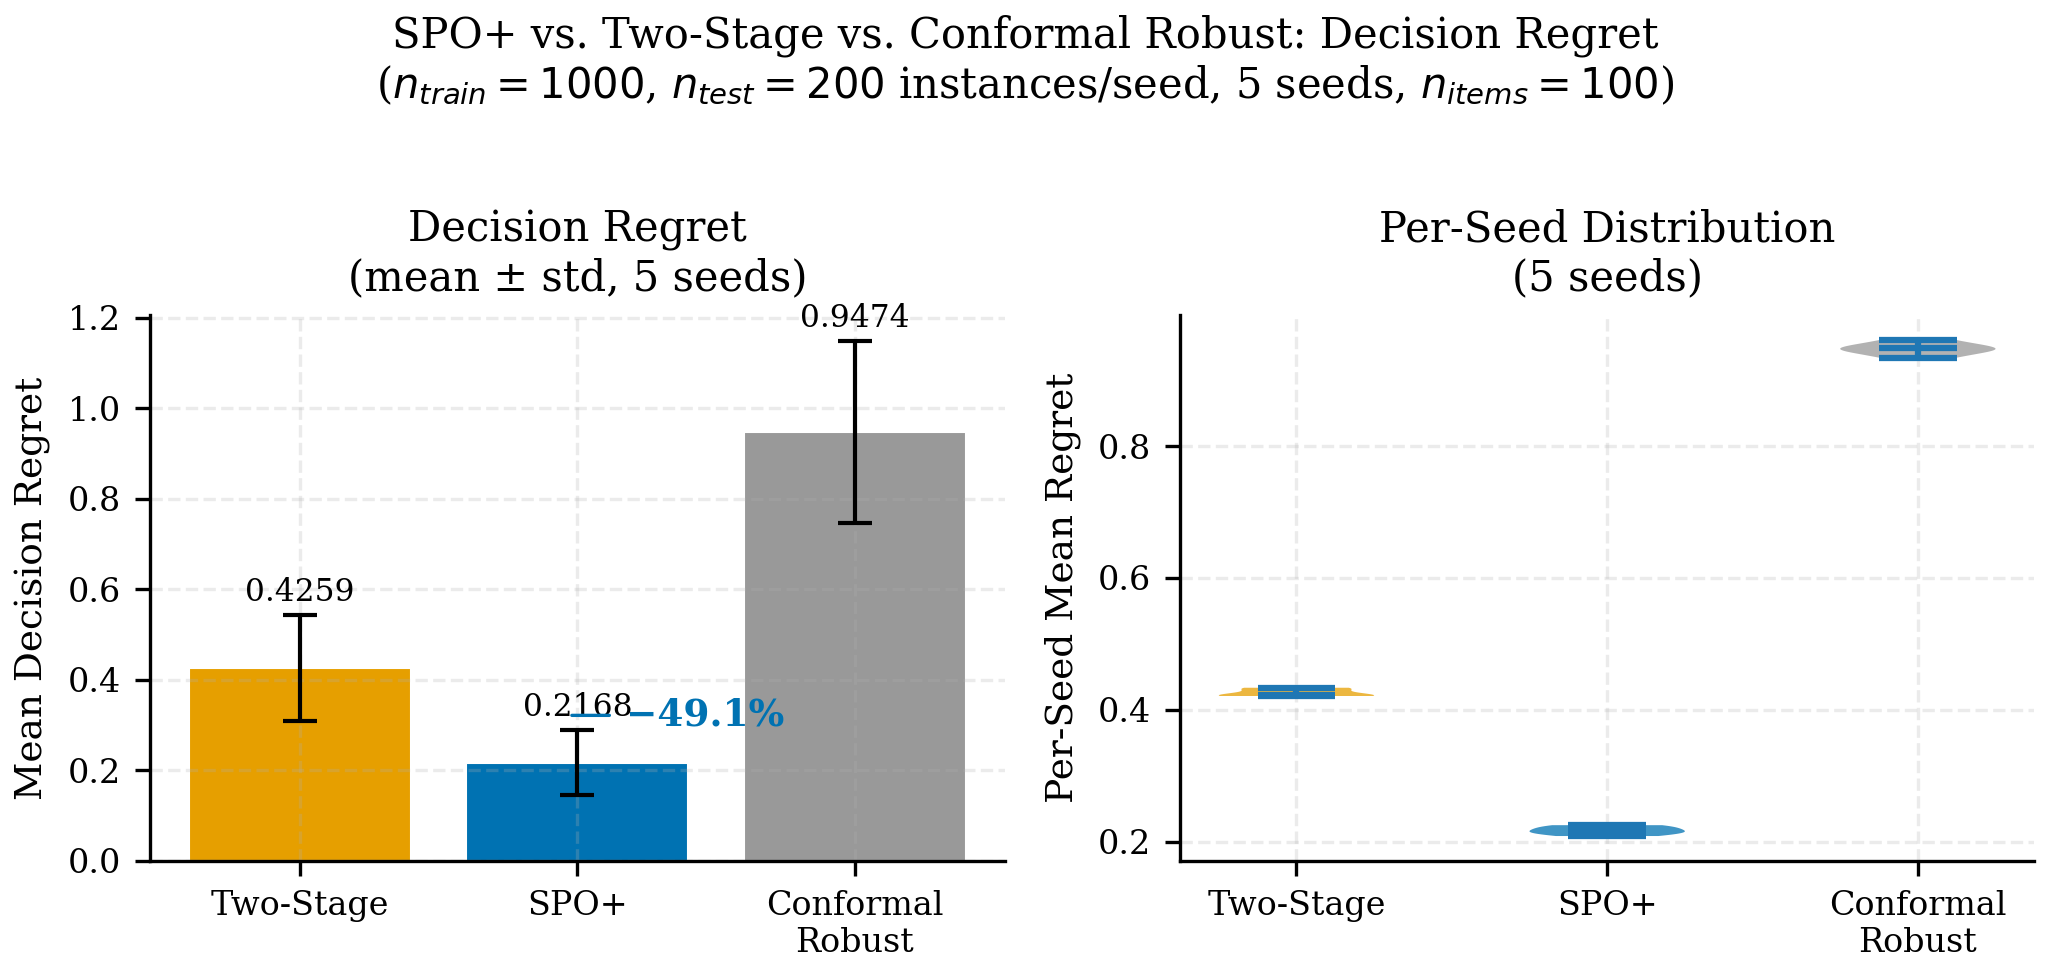
\includegraphics[keepaspectratio,alt={Comparación de regret para estrategias de optimización del Paper Estrella.}]{chapters/14-paper-estrella/../../assets/figures/publication/estrella_fig9_spo_regret.png}}

}

\caption{\label{fig-p1-spo-regret}Comparación de regret entre
estrategias predict-then-optimize y el enfoque robusto del Paper
Estrella.}

\end{figure}%

\end{minipage}%
%
\begin{minipage}[t]{0.50\linewidth}

\begin{figure}[H]

\centering{

\pandocbounded{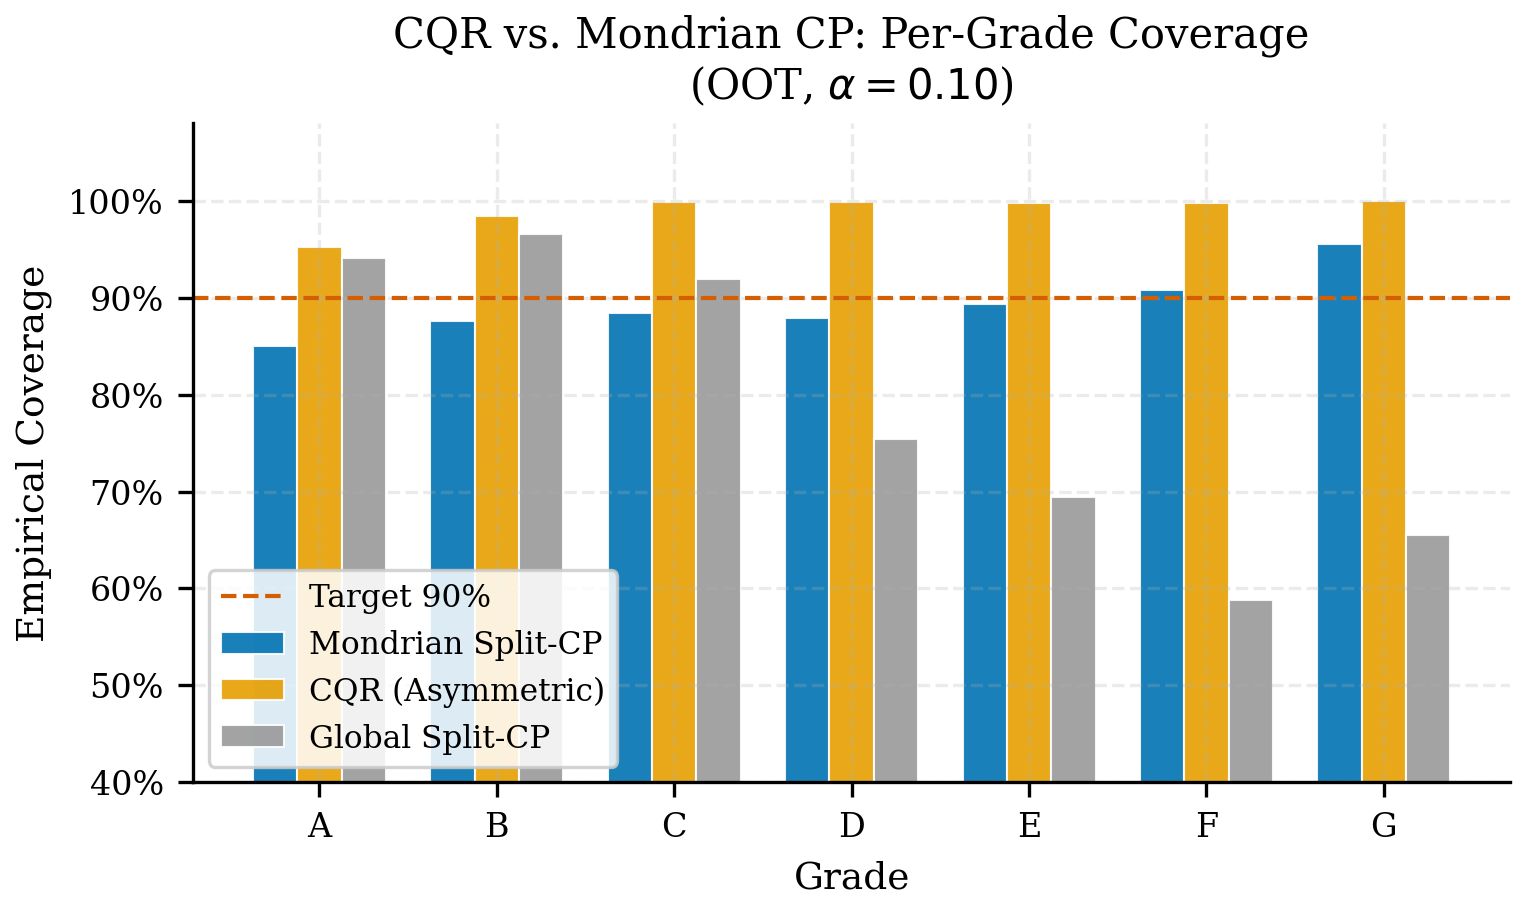
\includegraphics[keepaspectratio,alt={Cobertura conformal por grado para variantes evaluadas en el Paper Estrella.}]{chapters/14-paper-estrella/../../assets/figures/publication/estrella_fig10_cqr_per_grade.png}}

}

\caption{\label{fig-p1-cqr-grade}Cobertura por grado bajo CQR y
variantes conformales evaluadas en el Paper Estrella.}

\end{figure}%

\end{minipage}%

\end{figure*}%

\subsection{Frontera de alpha}\label{frontera-de-alpha}

El \emph{alpha sweep} muestra que subir confianza ensancha rápidamente
el conjunto y reduce la flexibilidad de decisión. Esa frontera es uno de
los hallazgos más útiles del paper porque convierte un hiperparámetro
estadístico en una palanca explícita de política económica.

\subsection{Lectura del conjunto de
resultados}\label{lectura-del-conjunto-de-resultados}

El hallazgo defendible no es ``la robustez siempre gana''. Es más
preciso:

\begin{enumerate}
\def\labelenumi{\arabic{enumi}.}
\tightlist
\item
  la incertidumbre conformal es suficientemente estable para entrar al
  optimizador;
\item
  frente a baselines alternativos, produce un conjunto más usable;
\item
  la calidad de la policy depende de cómo se negocia cobertura contra
  restricción económica.
\end{enumerate}

Ese matiz hace al paper más creíble y más útil para venues de OR o
\emph{analytics} aplicada.

\chapter{Discusión y Conclusiones}\label{sec-estrella-discussion}

El Paper Estrella articula la tesis más ambiciosa del proyecto:
convertir incertidumbre predictiva en un objeto directamente útil para
optimización de decisión. La evidencia actual ya permite sostener tres
conclusiones provisionales.

\subsection{Conclusiones}\label{conclusiones}

\begin{enumerate}
\def\labelenumi{\arabic{enumi}.}
\tightlist
\item
  Los intervalos conformales funcionan como conjuntos de incertidumbre
  operativos y trazables.
\item
  Frente a baselines simples, ofrecen mejor compromiso entre cobertura,
  anchura y estabilidad por grupo.
\item
  El nivel conformal puede interpretarse como una palanca de robustez
  con consecuencias económicas observables.
\end{enumerate}

\subsection{Threats to validity}\label{threats-to-validity}

La versión actual todavía enfrenta límites claros:

\begin{itemize}
\tightlist
\item
  el vínculo teórico \texttt{alpha\ ↔\ Gamma} requiere formalización
  completa;
\item
  el resultado económico depende de una policy y un run concretos;
\item
  faltan comparadores más ricos de decision-focused learning y robustez
  contextual.
\end{itemize}

\subsection{Reproducibility appendix}\label{reproducibility-appendix}

La reproducibilidad del paper está mejor resuelta que su cierre teórico.
El capítulo se apoya en:

\begin{itemize}
\tightlist
\item
  \texttt{data/processed/model\_comparison.json}
\item
  \texttt{data/processed/pipeline\_summary.json}
\item
  \texttt{data/processed/alpha\_sweep\_pareto\_both.parquet}
\item
  \texttt{data/processed/bma\_comparison.parquet}
\item
  \texttt{models/champion\_registry.json}
\end{itemize}

Además, la carpeta
\texttt{reports/paper\_material/figures\_publication/} conserva las
figuras editoriales congeladas para escritura y revisión.

\subsection{Próximo paso editorial}\label{pruxf3ximo-paso-editorial}

La mejor continuación no es expandir alcance indiscriminadamente, sino
endurecer el claim central con una versión journal:

\begin{enumerate}
\def\labelenumi{\arabic{enumi}.}
\tightlist
\item
  demostración formal más sólida;
\item
  benchmark adicional contra CRO y SPO+;
\item
  análisis de sensibilidad por segmento y periodo.
\end{enumerate}

Con eso, el paper quedaría bien posicionado como pieza bandera de la
agenda de maestría.

\chapter{Paper 2: IFRS9 End-to-End con Incertidumbre
Conformal}\label{paper-2-ifrs9-end-to-end-con-incertidumbre-conformal}

\begin{tcolorbox}[enhanced jigsaw, arc=.35mm, bottomrule=.15mm, bottomtitle=1mm, breakable, colback=white, colbacktitle=quarto-callout-important-color!10!white, colframe=quarto-callout-important-color-frame, coltitle=black, left=2mm, leftrule=.75mm, opacityback=0, opacitybacktitle=0.6, rightrule=.15mm, title=\textcolor{quarto-callout-important-color}{\faExclamation}\hspace{0.5em}{Paper autocontenido}, titlerule=0mm, toprule=.15mm, toptitle=1mm]

Esta sección funciona como un draft independiente del paper IFRS9.

\end{tcolorbox}

\chapter{Introducción}\label{sec-p2-intro}

IFRS9 obliga a convertir riesgo en provisión bajo una lógica prospectiva
y defendible. En la práctica, muchos pipelines siguen descansando en PD
puntuales y reglas SICR relativamente toscas. Este paper propone una
extensión concreta: incorporar incertidumbre conformal dentro de un
pipeline IFRS9 end-to-end.

\subsection{Problema}\label{problema}

Una PD puntual ordena riesgo, pero no informa cuánta confianza merece
esa estimación justo cuando la decisión contable se vuelve más sensible.
Esa limitación afecta tres frentes:

\begin{enumerate}
\def\labelenumi{\arabic{enumi}.}
\tightlist
\item
  staging (\texttt{Stage\ 1/2/3});
\item
  provisión esperada (\texttt{ECL});
\item
  sensibilidad ante escenarios macro y drift temporal.
\end{enumerate}

\subsection{Pregunta del paper}\label{pregunta-del-paper}

\begin{quote}
¿Cómo integrar incertidumbre distribution-free en un pipeline IFRS9 sin
romper trazabilidad, gobernanza ni interpretabilidad operacional?
\end{quote}

\subsection{Contribuciones}\label{contribuciones}

\begin{enumerate}
\def\labelenumi{\arabic{enumi}.}
\tightlist
\item
  ECL por rango usando PD puntual y bandas conformales.
\item
  Trigger SICR enriquecido con ancho conformal.
\item
  Sensibilidad explícita de provisiones frente a escenarios y parámetros
  prudenciales.
\end{enumerate}

\subsection{Relevancia de la brecha}\label{relevancia-de-la-brecha}

La revisión de \texttt{docs/PAPER\_REFERENCES\_STATE\_OF\_ART.md}
identifica un vacío notable: el proyecto no encontró papers que conecten
explícitamente conformal prediction con provisiones IFRS9 end-to-end.
Esa ausencia vuelve el caso más valioso, pero también exige una
escritura prudente y muy bien trazada.

\chapter{Metodología}\label{sec-p2-methodology}

La metodología reutiliza el stack productivo del proyecto y lo
reorganiza en clave de paper. El objetivo es mostrar que IFRS9 no es una
``aplicación lateral'', sino una consecuencia natural del pipeline de
riesgo ya construido.

\subsection{Componentes del pipeline}\label{componentes-del-pipeline}

\begin{longtable}[]{@{}
  >{\raggedright\arraybackslash}p{(\linewidth - 4\tabcolsep) * \real{0.3333}}
  >{\raggedright\arraybackslash}p{(\linewidth - 4\tabcolsep) * \real{0.3333}}
  >{\raggedright\arraybackslash}p{(\linewidth - 4\tabcolsep) * \real{0.3333}}@{}}
\caption{Capas metodológicas del Paper
2}\label{tbl-p2-method}\tabularnewline
\toprule\noalign{}
\begin{minipage}[b]{\linewidth}\raggedright
Capa
\end{minipage} & \begin{minipage}[b]{\linewidth}\raggedright
Artefacto principal
\end{minipage} & \begin{minipage}[b]{\linewidth}\raggedright
Rol
\end{minipage} \\
\midrule\noalign{}
\endfirsthead
\toprule\noalign{}
\begin{minipage}[b]{\linewidth}\raggedright
Capa
\end{minipage} & \begin{minipage}[b]{\linewidth}\raggedright
Artefacto principal
\end{minipage} & \begin{minipage}[b]{\linewidth}\raggedright
Rol
\end{minipage} \\
\midrule\noalign{}
\endhead
\bottomrule\noalign{}
\endlastfoot
PD calibrada & \texttt{data/processed/model\_comparison.json} &
probabilidad puntual defendible \\
Incertidumbre & \texttt{models/conformal\_policy\_status.json} & bandas
low/point/high \\
Escenarios IFRS9 &
\texttt{data/processed/ifrs9\_scenario\_summary.parquet} & provisiones
por severidad macro \\
Sensibilidad & \texttt{data/processed/ifrs9\_sensitivity\_grid.parquet}
& stress sobre PD, LGD y tasa \\
SICR & \texttt{scripts/run\_sicr\_conformal.py} + artefactos asociados &
trigger enriquecido por ancho \\
\end{longtable}

\subsection{Fórmula central}\label{fuxf3rmula-central}

La pérdida esperada por préstamo y escenario se resume como:

\[
\mathrm{ECL}_{i,s}^{(h)}=\mathrm{PD}_{i,s}^{(h)}\times \mathrm{LGD}_{i,s}\times \mathrm{EAD}_{i,s}\times \mathrm{DF}_{i,s},
\qquad h \in \{\text{low},\text{point},\text{high}\}
\]

La novedad práctica está en que \texttt{PD\^{}(h)} ya no es únicamente
puntual. El horizonte \texttt{high} define una lectura prudencial,
mientras \texttt{low} marca un piso de incertidumbre.

\subsection{Escenarios congelados}\label{escenarios-congelados}

El artefacto \texttt{ifrs9\_scenario\_summary.parquet} reporta cuatro
escenarios:

\begin{longtable}[]{@{}lrrr@{}}
\caption{Escenarios del Paper 2}\label{tbl-p2-scenarios}\tabularnewline
\toprule\noalign{}
Escenario & \texttt{pd\_mult} & \texttt{lgd\_mult} &
\texttt{discount\_rate} \\
\midrule\noalign{}
\endfirsthead
\toprule\noalign{}
Escenario & \texttt{pd\_mult} & \texttt{lgd\_mult} &
\texttt{discount\_rate} \\
\midrule\noalign{}
\endhead
\bottomrule\noalign{}
\endlastfoot
baseline & 1.0172 & 1.00 & 0.05 \\
mild\_stress & 1.1697 & 1.05 & 0.06 \\
adverse & 1.3223 & 1.12 & 0.07 \\
severe & 1.5766 & 1.20 & 0.08 \\
\end{longtable}

\subsection{Trigger SICR con
incertidumbre}\label{trigger-sicr-con-incertidumbre}

El capítulo de SICR mostró una regla complementaria basada en ancho
conformal. Conceptualmente:

\[
\mathrm{Stage2}_i=\mathbb{1}\left[\Delta \widehat{PD}_i>\theta_{PD}\;\lor\;(w_i>t \wedge \Delta \widehat{PD}_i \ge 0)\right]
\]

Esto permite capturar deterioro potencial aun cuando la PD puntual no
cruce el umbral absoluto clásico.

\subsection{Protocolo de evaluación}\label{protocolo-de-evaluaciuxf3n}

El paper reporta:

\begin{enumerate}
\def\labelenumi{\arabic{enumi}.}
\tightlist
\item
  ECL agregado por escenario;
\item
  composición de stages;
\item
  efecto del trigger SICR conformal;
\item
  sensibilidad a parámetros prudenciales y extensiones con riesgos
  competitivos.
\end{enumerate}

\chapter{Resultados}\label{sec-p2-results}

Los resultados muestran que IFRS9 es el lugar donde la incertidumbre
deja de ser una curiosidad estadística y se convierte en un costo
prudencial observable.

\subsection{ECL por escenario}\label{ecl-por-escenario}

El agregado congelado es:

\begin{longtable}[]{@{}lrrrr@{}}
\caption{IFRS9 por escenario}\label{tbl-p2-results}\tabularnewline
\toprule\noalign{}
Escenario & Total ECL & Stage 1 & Stage 2 & Stage 3 \\
\midrule\noalign{}
\endfirsthead
\toprule\noalign{}
Escenario & Total ECL & Stage 1 & Stage 2 & Stage 3 \\
\midrule\noalign{}
\endhead
\bottomrule\noalign{}
\endlastfoot
baseline & \$1.003B & 85,659 & 128,959 & 62,251 \\
mild\_stress & \$1.223B & 58,059 & 156,559 & 62,251 \\
adverse & \$1.454B & 47,218 & 167,400 & 62,251 \\
severe & \$1.799B & 30,019 & 184,599 & 62,251 \\
\end{longtable}

El salto de baseline a severe implica aproximadamente +79\% de ECL. Esa
sensibilidad es suficiente para justificar una lectura prudencial
explícita del escenario y no solo un reporte puntual de provisión.

\begin{figure*}

\begin{minipage}[t]{0.50\linewidth}

\begin{figure}[H]

\centering{

\pandocbounded{\includegraphics[keepaspectratio,alt={Grid de escenarios y reglas SICR del paper IFRS9.}]{chapters/15-paper-ifrs9/../../assets/figures/publication/p2_fig4_sicr_grid.png}}

}

\caption{\label{fig-p2-sicr-grid}Grid de escenarios SICR y staging
conformal usado en el paper IFRS9.}

\end{figure}%

\end{minipage}%
%
\begin{minipage}[t]{0.50\linewidth}

\begin{figure}[H]

\centering{

\pandocbounded{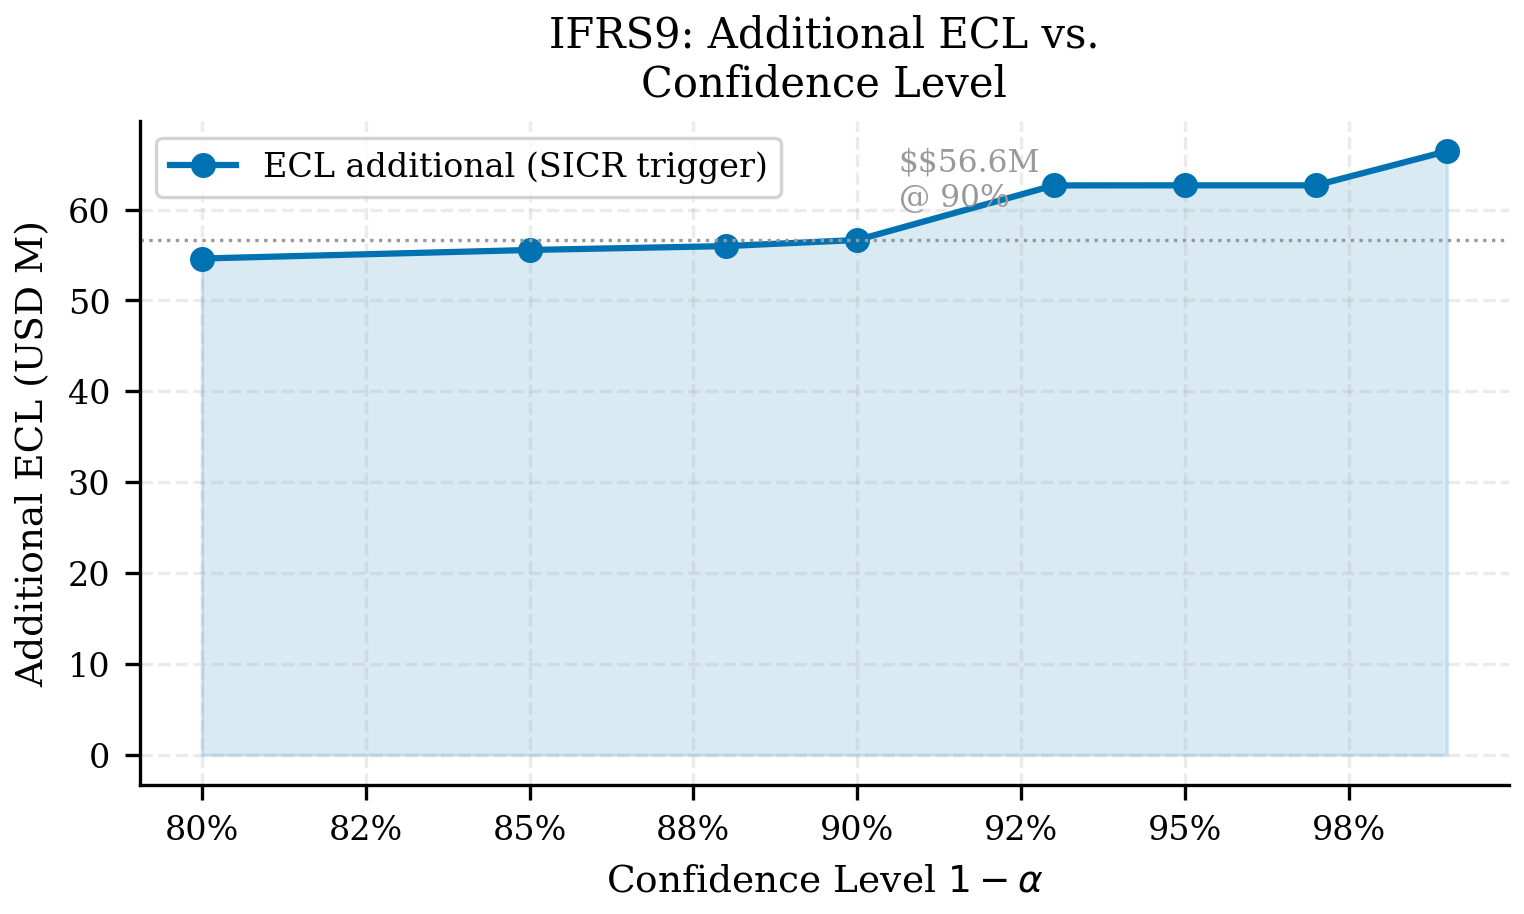
\includegraphics[keepaspectratio,alt={Sensibilidad del ECL al parámetro alpha en el paper IFRS9.}]{chapters/15-paper-ifrs9/../../assets/figures/publication/p2_fig5_ecl_alpha_sensitivity.png}}

}

\caption{\label{fig-p2-ecl-alpha}Sensibilidad del ECL al barrido de
alpha y al endurecimiento prudencial del escenario.}

\end{figure}%

\end{minipage}%

\end{figure*}%

\subsection{SICR con ancho conformal}\label{sicr-con-ancho-conformal}

El trigger complementario basado en incertidumbre encuentra un óptimo
útil en \texttt{t*\ =\ 0.30} para \texttt{pd\_threshold\ =\ 0.20}, con:

\begin{longtable}[]{@{}lr@{}}
\caption{Resultado operativo de SICR
conformal}\label{tbl-p2-sicr}\tabularnewline
\toprule\noalign{}
Indicador & Valor \\
\midrule\noalign{}
\endfirsthead
\toprule\noalign{}
Indicador & Valor \\
\midrule\noalign{}
\endhead
\bottomrule\noalign{}
\endlastfoot
F1 & 0.2515 \\
Recall de defaults no capturados & 75.8\% \\
Precisión & 8.9\% \\
ECL adicional & \$56.6M \\
\end{longtable}

La precisión baja es consistente con una política prudencial: el
mecanismo privilegia no dejar escapar deterioros potenciales, aun a
costa de sobreclasificar ciertos casos a Stage 2.

\begin{figure*}

\centering{

\pandocbounded{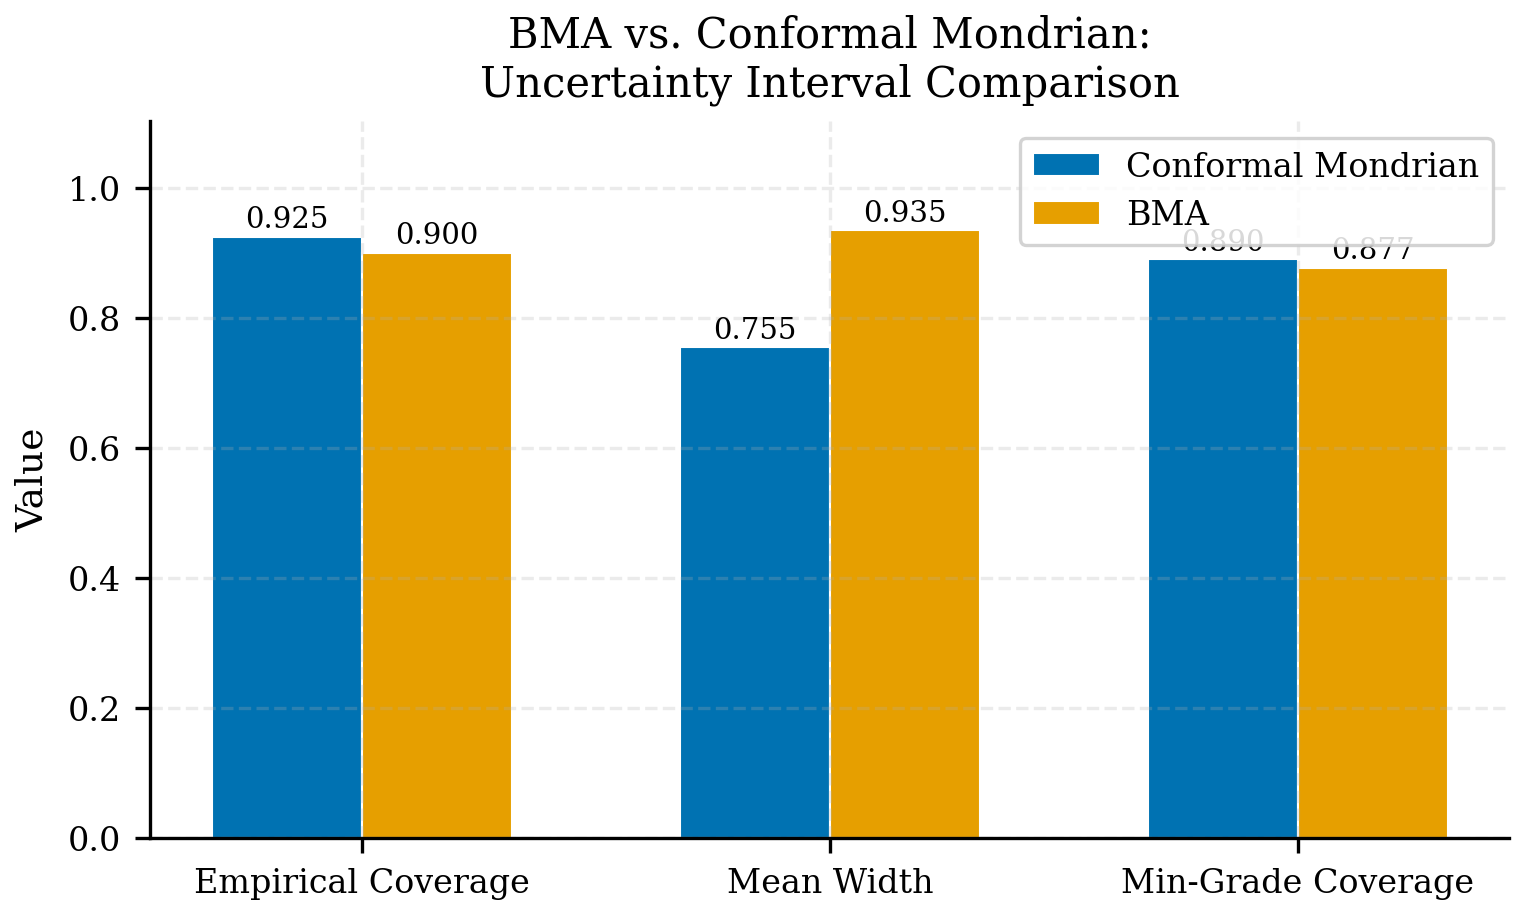
\includegraphics[keepaspectratio,alt={Comparación entre BMA y predicción conformal en el paper IFRS9.}]{chapters/15-paper-ifrs9/../../assets/figures/publication/p2_fig6_bma_vs_cp.png}}

}

\caption{\label{fig-p2-bma-vs-cp}Comparación entre Bayesian Model
Averaging y Conformal Prediction en amplitud de banda y lectura
prudencial para IFRS9.}

\end{figure*}%

\subsection{Sensibilidad
metodológica}\label{sensibilidad-metodoluxf3gica}

Las extensiones del libro refuerzan esta lectura:

\begin{itemize}
\tightlist
\item
  el análisis de costos por misclasificación ubica óptimos de threshold
  lejos de soluciones intuitivas;
\item
  el capítulo de riesgos competitivos muestra que el método de
  supervivencia puede mover Stage 2 ECL en decenas de millones;
\item
  el capítulo temporal evidencia que la incertidumbre macro puede
  expandir fuertemente el rango de provisión.
\end{itemize}

\subsection{Lectura del paper}\label{lectura-del-paper}

El resultado fuerte no es que exista una única provisión ``correcta''.
Es que el pipeline puede exponer de forma trazable:

\begin{enumerate}
\def\labelenumi{\arabic{enumi}.}
\tightlist
\item
  una provisión puntual;
\item
  una banda prudencial;
\item
  el costo de endurecer staging y escenario.
\end{enumerate}

Eso es exactamente el tipo de capacidad que un comité de finanzas y
riesgo puede usar.

\chapter{Discusión}\label{sec-p2-discussion}

El Paper 2 muestra que IFRS9 puede funcionar como el caso de uso más
convincente para incertidumbre conformal en finanzas aplicadas. La razón
es simple: allí la incertidumbre afecta dinero, provisión y gobernanza a
la vez.

\subsection{Conclusiones principales}\label{conclusiones-principales}

\begin{enumerate}
\def\labelenumi{\arabic{enumi}.}
\tightlist
\item
  El pipeline produce ECL por escenario con trazabilidad suficiente para
  análisis prudencial.
\item
  El ancho conformal es una señal útil para enriquecer SICR, no solo una
  métrica técnica.
\item
  La sensibilidad del sistema a escenario, threshold y método de
  supervivencia justifica una política explícita de gobernanza.
\end{enumerate}

\subsection{Threats to validity}\label{threats-to-validity-1}

\begin{itemize}
\tightlist
\item
  Lending Club no es un banco regulado ni una cartera IFRS9 real.
\item
  La regla SICR conformal aún debe contrastarse con políticas expertas
  más ricas.
\item
  La integración de forecasting temporal y competing risks sigue en modo
  analítico, no productivo pleno.
\end{itemize}

\subsection{Reproducibility appendix}\label{reproducibility-appendix-1}

Los resultados se apoyan en artefactos ya existentes:

\begin{itemize}
\tightlist
\item
  \texttt{data/processed/ifrs9\_scenario\_summary.parquet}
\item
  \texttt{data/processed/ifrs9\_sensitivity\_grid.parquet}
\item
  \texttt{data/processed/cif\_ecl\_impact.parquet}
\item
  \texttt{data/processed/stage\_misclassification\_cost.parquet}
\item
  \texttt{data/processed/ts\_ecl\_intervals.parquet}
\end{itemize}

\subsection{Cierre editorial}\label{cierre-editorial}

La contribución más defendible del paper es que convierte IFRS9 en un
pipeline cuantitativo gobernable, donde provisión, incertidumbre y señal
de deterioro pueden discutirse con evidencia compartida. Esa es una
propuesta mucho más valiosa que un ejercicio aislado de lifetime PD.

\chapter{Paper 3: Predicción Conformal Mondrian para Riesgo
Crediticio}\label{paper-3-predicciuxf3n-conformal-mondrian-para-riesgo-crediticio}

\begin{tcolorbox}[enhanced jigsaw, arc=.35mm, bottomrule=.15mm, bottomtitle=1mm, breakable, colback=white, colbacktitle=quarto-callout-important-color!10!white, colframe=quarto-callout-important-color-frame, coltitle=black, left=2mm, leftrule=.75mm, opacityback=0, opacitybacktitle=0.6, rightrule=.15mm, title=\textcolor{quarto-callout-important-color}{\faExclamation}\hspace{0.5em}{Paper autocontenido}, titlerule=0mm, toprule=.15mm, toptitle=1mm]

Esta sección funciona como un draft independiente del paper Mondrian
para COPA 2026.

\end{tcolorbox}

\chapter{Introducción}\label{sec-p3-intro}

La cobertura marginal global puede ser una garantía engañosa en riesgo
crediticio. Un modelo puede cubrir ``en promedio'' y, al mismo tiempo,
fallar sistemáticamente en segmentos económicamente relevantes. Este
paper toma esa tensión como problema central y evalúa Mondrian conformal
sobre particiones naturales del portafolio.

\subsection{Problema}\label{problema-1}

En Lending Club, los grades A-G no son una conveniencia estadística; son
segmentos con semántica de negocio y gradiente de riesgo visible. Si la
cobertura cae precisamente en los grupos más riesgosos o más pequeños,
la garantía global pierde valor operacional.

\subsection{Pregunta del paper}\label{pregunta-del-paper-1}

\begin{quote}
¿Puede Mondrian conformal ofrecer cobertura útil por subgrupo en crédito
real sin inflar excesivamente la anchura de los intervalos?
\end{quote}

\subsection{Contribuciones}\label{contribuciones-1}

\begin{enumerate}
\def\labelenumi{\arabic{enumi}.}
\tightlist
\item
  Evalúa cobertura por grupo en una ventana OOT real.
\item
  Compara variantes conformales globales y particionadas.
\item
  Propone una lectura de monitoreo temporal y de alertas para uso
  operativo.
\end{enumerate}

\subsection{Posicionamiento}\label{posicionamiento}

El paper no compite por inventar una nueva variante conformal. Su fuerza
está en la evaluación aplicada, reproducible y conectada con downstream
tasks del mismo proyecto.

\chapter{Metodología}\label{sec-p3-methodology}

La metodología parte del pipeline PD calibrado y estudia varias capas de
evaluación conformal sobre el mismo split OOT congelado. El objetivo es
medir no solo cobertura agregada, sino cobertura útil por grupo y por
tiempo.

\subsection{Definición básica}\label{definiciuxf3n-buxe1sica}

El intervalo Mondrian por grupo se escribe como:

\[
\widehat{C}_{1-\alpha}(x,g)=\left[\max\{0,\widehat{p}(x)-q_{1-\alpha,g}\},\min\{1,\widehat{p}(x)+q_{1-\alpha,g}\}\right]
\]

donde \texttt{g} representa la partición seleccionada. En la narrativa
del proyecto, \texttt{grade} es la partición más interpretable, aunque
también se contrastan variantes por score-space.

\subsection{Protocolo de evaluación}\label{protocolo-de-evaluaciuxf3n-1}

\begin{longtable}[]{@{}
  >{\raggedright\arraybackslash}p{(\linewidth - 4\tabcolsep) * \real{0.3333}}
  >{\raggedright\arraybackslash}p{(\linewidth - 4\tabcolsep) * \real{0.3333}}
  >{\raggedright\arraybackslash}p{(\linewidth - 4\tabcolsep) * \real{0.3333}}@{}}
\caption{Diseño metodológico del Paper
3}\label{tbl-p3-method}\tabularnewline
\toprule\noalign{}
\begin{minipage}[b]{\linewidth}\raggedright
Capa
\end{minipage} & \begin{minipage}[b]{\linewidth}\raggedright
Artefacto
\end{minipage} & \begin{minipage}[b]{\linewidth}\raggedright
Qué mide
\end{minipage} \\
\midrule\noalign{}
\endfirsthead
\toprule\noalign{}
\begin{minipage}[b]{\linewidth}\raggedright
Capa
\end{minipage} & \begin{minipage}[b]{\linewidth}\raggedright
Artefacto
\end{minipage} & \begin{minipage}[b]{\linewidth}\raggedright
Qué mide
\end{minipage} \\
\midrule\noalign{}
\endhead
\bottomrule\noalign{}
\endlastfoot
Cobertura global & \texttt{models/conformal\_policy\_status.json} &
validez agregada \\
Benchmark de variantes &
\texttt{conformal\_variant\_selection\_report.parquet} & trade-off entre
métodos \\
Backtest mensual & artefactos conformales del proyecto & estabilidad
temporal \\
Guardrails & checks de policy & elegibilidad de promoción \\
\end{longtable}

\subsection{Métricas principales}\label{muxe9tricas-principales}

\begin{enumerate}
\def\labelenumi{\arabic{enumi}.}
\tightlist
\item
  cobertura al 90\% y 95\%;
\item
  cobertura mínima por grupo;
\item
  ancho medio;
\item
  alertas estadísticas y no estadísticas;
\item
  estabilidad mensual bajo drift temporal.
\end{enumerate}

\subsection{Comparadores}\label{comparadores}

El benchmark del capítulo base ya deja una línea de referencia
importante:

\begin{itemize}
\tightlist
\item
  el \emph{global split} puede quedar con cobertura mínima por grupo
  cercana a 59.5\%;
\item
  variantes Mondrian y score-decile mejoran esa situación a costa de
  mayor complejidad o anchura.
\end{itemize}

La metodología del paper aprovecha esa comparación para justificar por
qué la garantía por grupo importa más que un promedio agregado cómodo.

\chapter{Resultados}\label{sec-p3-results}

El resultado central del Paper 3 es que la cobertura global del sistema
es fuerte, pero su interpretación correcta exige mirar la capa por grupo
y la capa temporal.

\subsection{Estado agregado del
sistema}\label{estado-agregado-del-sistema}

\begin{longtable}[]{@{}lr@{}}
\caption{Resumen conformal del Paper
3}\label{tbl-p3-core}\tabularnewline
\toprule\noalign{}
Indicador & Valor \\
\midrule\noalign{}
\endfirsthead
\toprule\noalign{}
Indicador & Valor \\
\midrule\noalign{}
\endhead
\bottomrule\noalign{}
\endlastfoot
Cobertura 90\% & 92.52\% \\
Cobertura 95\% & 95.93\% \\
Min group coverage 90\% & 89.01\% \\
Checks aprobados & 9 / 13 \\
\texttt{overall\_pass} & \texttt{False} \\
\end{longtable}

La clave está en que la cobertura útil por grupo sigue siendo alta,
incluso cuando la policy estricta mantiene alertas estadísticas de
backtesting.

\begin{figure*}

\begin{minipage}[t]{0.50\linewidth}

\begin{figure}[H]

\centering{

\pandocbounded{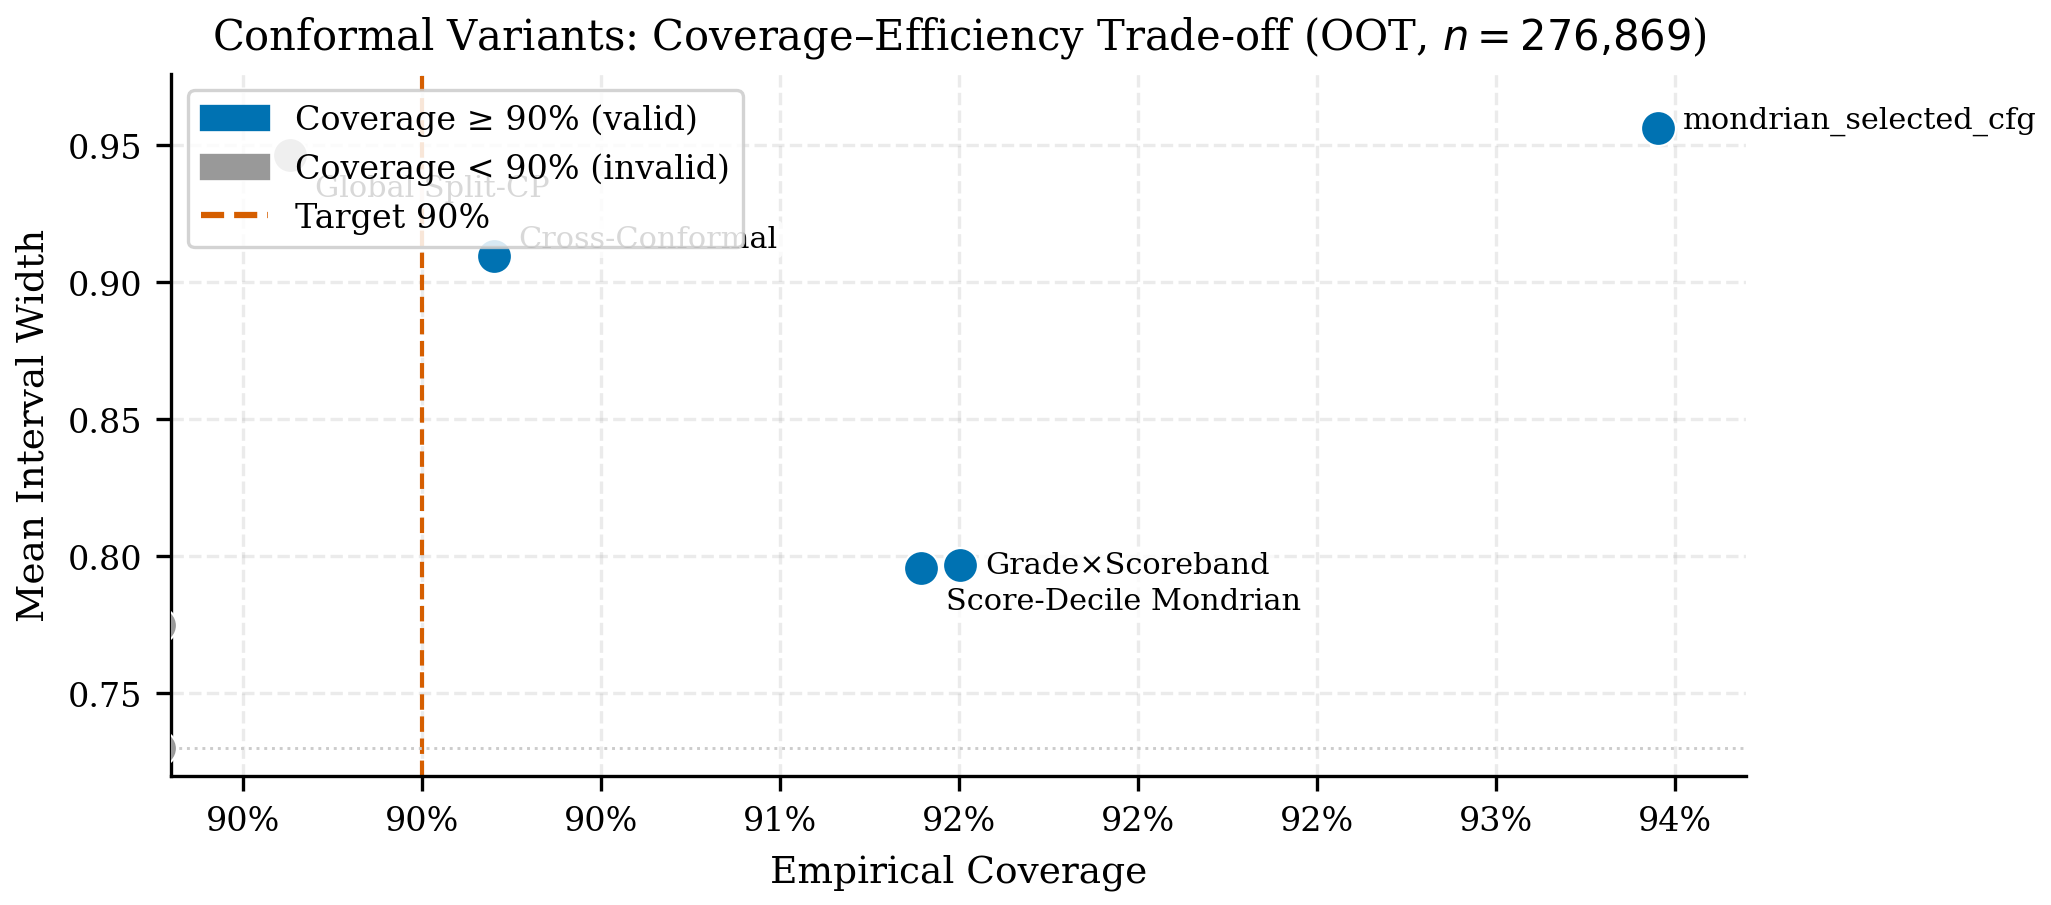
\includegraphics[keepaspectratio,alt={Scatter de variantes conformales comparando cobertura y anchura en el Paper Mondrian.}]{chapters/16-paper-mondrian/../../assets/figures/publication/p3_fig1_variant_scatter.png}}

}

\caption{\label{fig-p3-variant-scatter}Scatter de variantes conformales
del Paper 3, con énfasis en cobertura útil y costo de anchura.}

\end{figure}%

\end{minipage}%
%
\begin{minipage}[t]{0.50\linewidth}

\begin{figure}[H]

\centering{

\pandocbounded{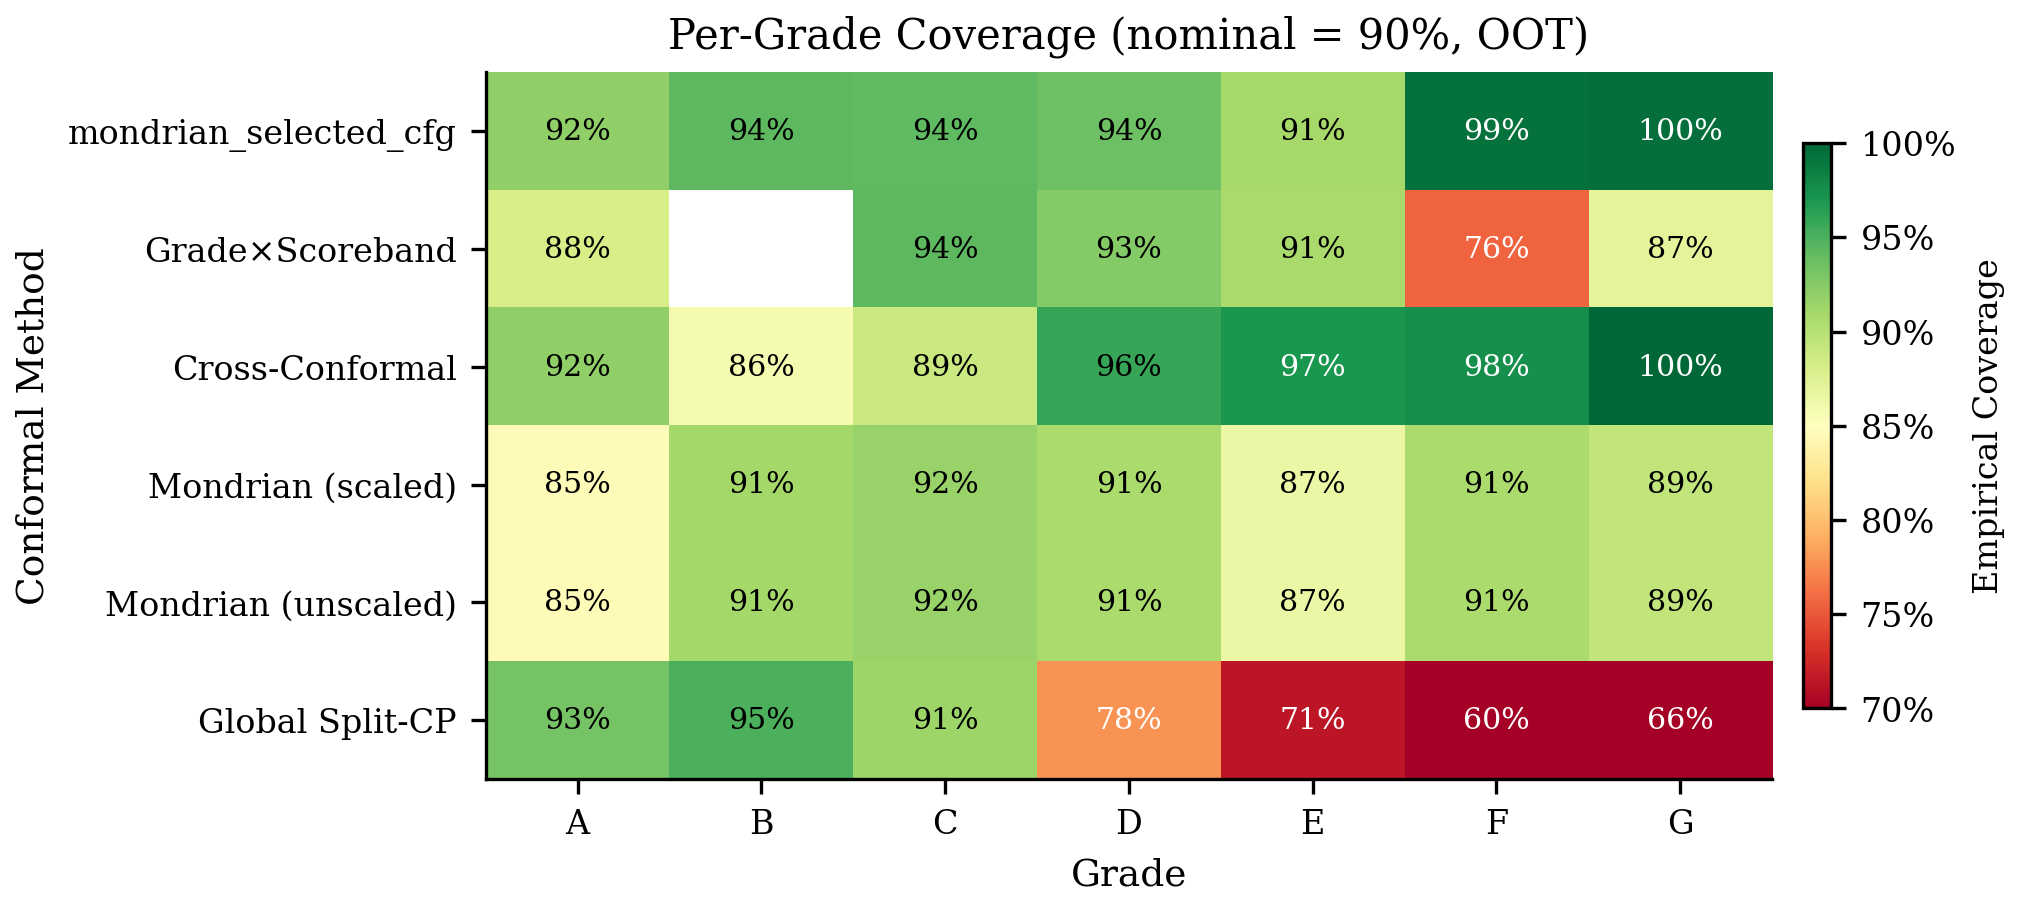
\includegraphics[keepaspectratio,alt={Mapa de calor de cobertura por grade en el Paper Mondrian.}]{chapters/16-paper-mondrian/../../assets/figures/publication/p3_fig2_grade_coverage_heatmap.png}}

}

\caption{\label{fig-p3-grade-heatmap}Mapa de calor de cobertura por
grade para la variante Mondrian promovida.}

\end{figure}%

\end{minipage}%

\end{figure*}%

\subsection{Qué enseñan las
alertas}\label{quuxe9-enseuxf1an-las-alertas}

Las fallas activas están concentradas en Kupiec y Christoffersen. Eso
significa que el sistema no debe presentarse como ``perfectamente
validado'' en sentido clásico de tests de independencia, pero sí como un
framework donde la garantía principal y la gobernanza de alertas ya
están explícitas.

\subsection{Comparación contra variantes más
simples}\label{comparaciuxf3n-contra-variantes-muxe1s-simples}

El benchmark base ya documentó que el \emph{global split} puede lograr
cobertura marginal aceptable con cobertura mínima por grupo inaceptable.
Ese contraste fortalece la tesis del paper:

\begin{quote}
En crédito, la validez útil no es solo marginal; debe sobrevivir a
particiones con significado de negocio.
\end{quote}

\subsection{Lectura operativa}\label{lectura-operativa}

Para el proyecto, el valor de Mondrian no es puramente teórico. Permite:

\begin{enumerate}
\def\labelenumi{\arabic{enumi}.}
\tightlist
\item
  alimentar IFRS9 y portafolio con una incertidumbre segmentada;
\item
  monitorear si ciertos grupos empiezan a perder garantía antes que
  otros;
\item
  justificar una elección metodológica frente a revisores exigentes.
\end{enumerate}

\subsection{Resultado editorial}\label{resultado-editorial}

La evidencia actual es suficiente para escribir un paper aplicado
sólido, aun si queda trabajo por hacer en endurecimiento temporal y
pruebas adicionales de estabilidad.

\begin{figure*}

\centering{

\pandocbounded{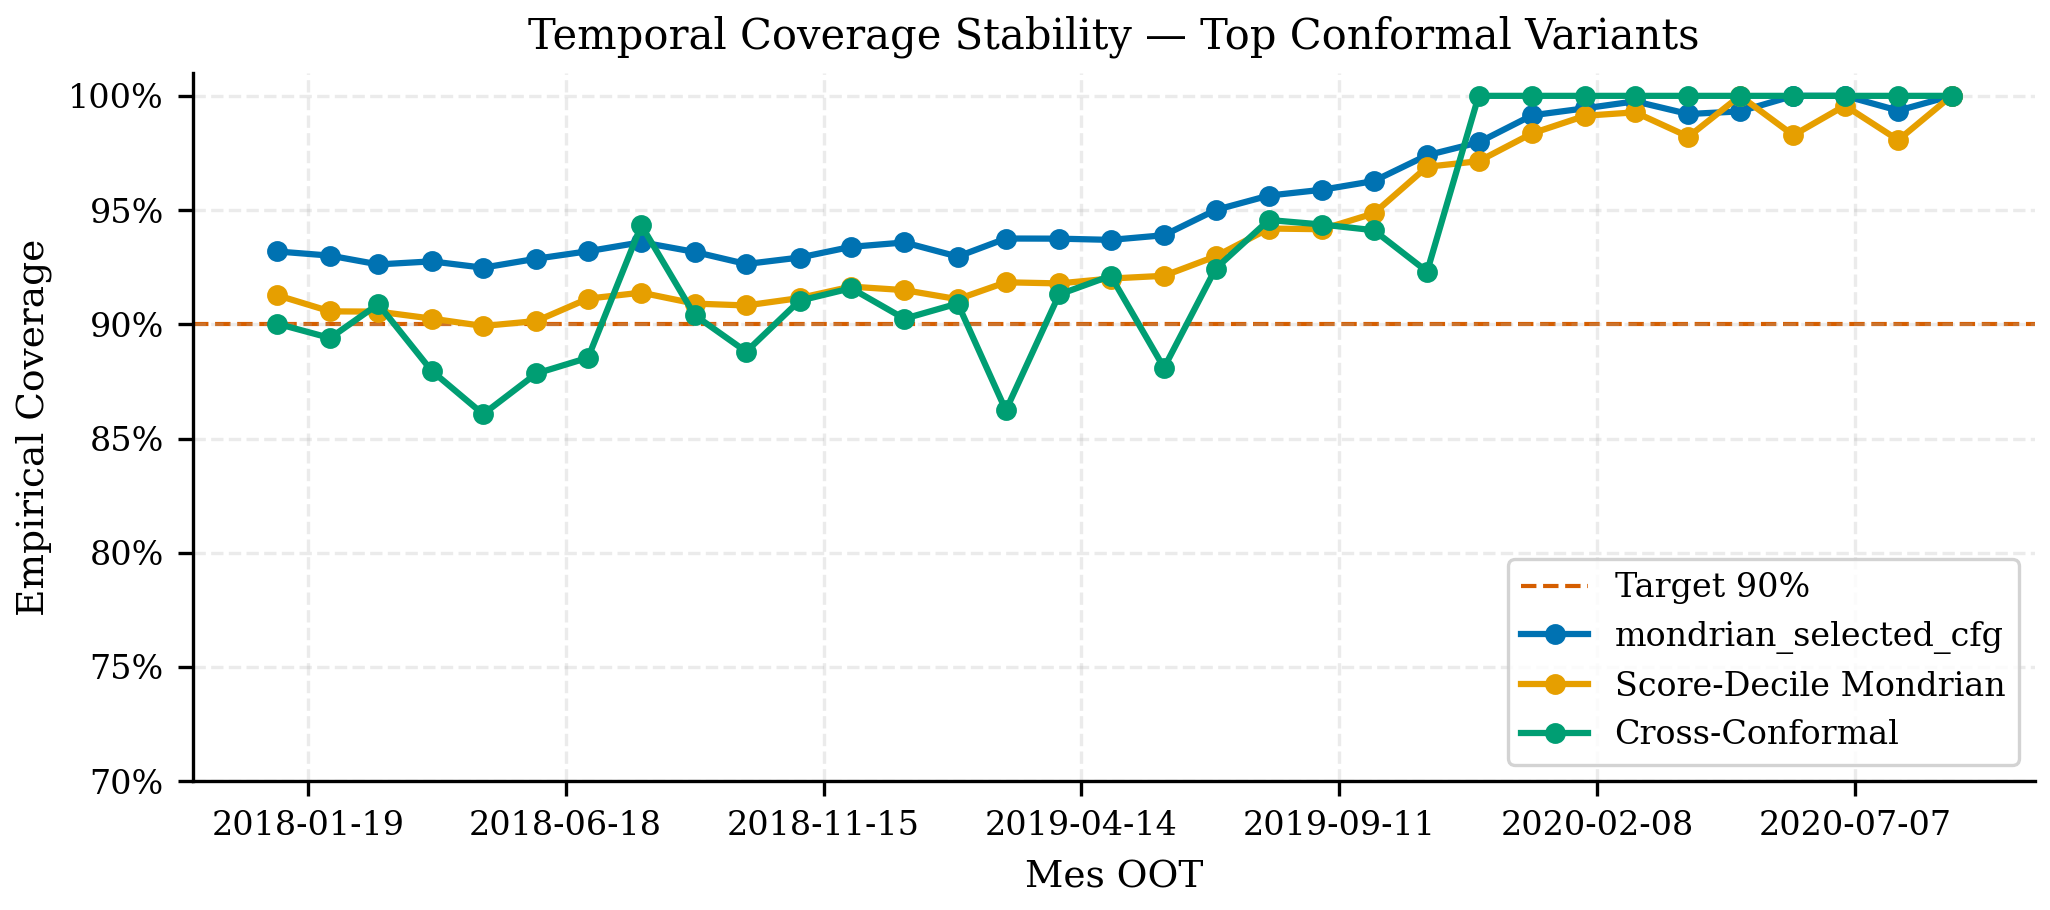
\includegraphics[keepaspectratio,alt={Gráfico de estabilidad temporal de la cobertura conformal en el Paper Mondrian.}]{chapters/16-paper-mondrian/../../assets/figures/publication/p3_fig3_temporal_stability.png}}

}

\caption{\label{fig-p3-temporal-stability}Estabilidad temporal de la
cobertura conformal, usada para documentar alertas y drift en el Paper
3.}

\end{figure*}%

\chapter{Discusión}\label{sec-p3-discussion}

El Paper 3 aporta una pieza metodológica importante a toda la agenda del
proyecto: sin cobertura por grupo razonablemente estable, la conexión
con IFRS9, optimización o gobernanza se vuelve más frágil.

\subsection{Conclusiones}\label{conclusiones-1}

\begin{enumerate}
\def\labelenumi{\arabic{enumi}.}
\tightlist
\item
  Mondrian conformal mejora de forma material la utilidad de la garantía
  en segmentos de crédito.
\item
  La cobertura global del sistema es buena, pero su defensa depende de
  exponer abiertamente las alertas estadísticas remanentes.
\item
  El enfoque ya es suficientemente reproducible para un paper aplicado
  con valor propio.
\end{enumerate}

\subsection{Threats to validity}\label{threats-to-validity-2}

\begin{itemize}
\tightlist
\item
  la partición por \texttt{grade} es fuerte en interpretación, pero no
  necesariamente óptima en eficiencia;
\item
  la estabilidad temporal debería evaluarse con ventanas más largas y
  reglas de recalibración más explícitas;
\item
  faltan más comparadores recientes de cobertura aproximadamente
  condicional.
\end{itemize}

\subsection{Reproducibility appendix}\label{reproducibility-appendix-2}

La evidencia del paper se ancla en:

\begin{itemize}
\tightlist
\item
  \texttt{models/conformal\_policy\_status.json}
\item
  \texttt{data/processed/conformal\_variant\_selection\_report.parquet}
\item
  artefactos de backtesting y monitoreo conformal del proyecto
\item
  \texttt{docs/PAPER\_REFERENCES\_STATE\_OF\_ART.md}
\end{itemize}

\subsection{Cierre}\label{cierre}

El valor final del paper es doble: produce una contribución autónoma
sobre cobertura por subgrupo en crédito y, al mismo tiempo, sostiene
metodológicamente los otros dos papers de la agenda.

\part{Parte V: Puente Académico y Agenda}

\chapter{Puente: De la Especialización a la
Maestría}\label{puente-de-la-especializaciuxf3n-a-la-maestruxeda}

Este capítulo evita una ruptura artificial entre dos etapas académicas
del proyecto. La especialización no queda como un prototipo aislado y la
maestría no arranca desde cero: ambas comparten artefactos, lenguaje
metodológico y trazabilidad.

\subsection{Qué queda cerrado en la
especialización}\label{quuxe9-queda-cerrado-en-la-especializaciuxf3n}

El documento espejo \texttt{reports/tesis\_especializacion.md} deja
claro que la fase de especialización ya consolidó una columna vertebral
defendible:

\begin{longtable}[]{@{}ll@{}}
\caption{Cierre de
especialización}\label{tbl-bridge-specialization}\tabularnewline
\toprule\noalign{}
Componente & Estado narrativo \\
\midrule\noalign{}
\endfirsthead
\toprule\noalign{}
Componente & Estado narrativo \\
\midrule\noalign{}
\endhead
\bottomrule\noalign{}
\endlastfoot
Dataset y split temporal & cerrados y trazables \\
PD calibrada & consolidada \\
Conformal PD/LGD/EAD & disponible con artefactos \\
IFRS9 por escenarios & operativo como capa analítica \\
Fairness y gobernanza & reportados explícitamente \\
\end{longtable}

La tesis de especialización, entonces, no termina con ``ideas
prometedoras'', sino con evidencia suficiente para una defensa seria y
un paquete reproducible.

\subsection{Qué cambia al entrar a
maestría}\label{quuxe9-cambia-al-entrar-a-maestruxeda}

La maestría no necesita rehacer el stack base. Lo que cambia es el nivel
de ambición científica:

\begin{enumerate}
\def\labelenumi{\arabic{enumi}.}
\tightlist
\item
  pasar de implementación aplicada a claims publicables;
\item
  endurecer demostraciones, comparadores y threats to validity;
\item
  separar el material en piezas autocontenidas tipo paper.
\end{enumerate}

\subsection{Tres líneas de continuidad
natural}\label{tres-luxedneas-de-continuidad-natural}

\begin{longtable}[]{@{}
  >{\raggedright\arraybackslash}p{(\linewidth - 4\tabcolsep) * \real{0.3333}}
  >{\raggedright\arraybackslash}p{(\linewidth - 4\tabcolsep) * \real{0.3333}}
  >{\raggedright\arraybackslash}p{(\linewidth - 4\tabcolsep) * \real{0.3333}}@{}}
\caption{Continuidad temática especialización →
maestría}\label{tbl-bridge-masters}\tabularnewline
\toprule\noalign{}
\begin{minipage}[b]{\linewidth}\raggedright
Línea
\end{minipage} & \begin{minipage}[b]{\linewidth}\raggedright
Herencia desde especialización
\end{minipage} & \begin{minipage}[b]{\linewidth}\raggedright
Expansión en maestría
\end{minipage} \\
\midrule\noalign{}
\endfirsthead
\toprule\noalign{}
\begin{minipage}[b]{\linewidth}\raggedright
Línea
\end{minipage} & \begin{minipage}[b]{\linewidth}\raggedright
Herencia desde especialización
\end{minipage} & \begin{minipage}[b]{\linewidth}\raggedright
Expansión en maestría
\end{minipage} \\
\midrule\noalign{}
\endhead
\bottomrule\noalign{}
\endlastfoot
Predict-then-optimize & PD calibrada + CP + portafolio & Paper
Estrella \\
IFRS9 con incertidumbre & ECL, escenarios y SICR & Paper 2 \\
Cobertura por subgrupo & Mondrian y backtesting & Paper 3 \\
\end{longtable}

\subsection{Por qué este puente es
defendible}\label{por-quuxe9-este-puente-es-defendible}

El proyecto ya cuenta con señales de madurez poco comunes para un
trabajo de transición:

\begin{itemize}
\tightlist
\item
  \texttt{638} pruebas registradas en \texttt{runtime\_status.json};
\item
  \texttt{30} páginas Streamlit temáticas;
\item
  registro de campeón y semántica de thresholds congelados;
\item
  manifests de notebooks y artefactos reutilizables.
\end{itemize}

Esto no elimina el trabajo futuro, pero sí cambia su naturaleza: el
esfuerzo se desplaza desde ``construir'' hacia ``formalizar, comparar y
publicar''.

\subsection{Regla editorial del
puente}\label{regla-editorial-del-puente}

La especialización conserva protagonismo como cierre defendible. La
maestría aparece como continuidad orgánica, no como excusa para posponer
el cierre. Ese equilibrio importa tanto para jurados como para
directores:

\begin{itemize}
\tightlist
\item
  lo ya construido tiene valor autónomo;
\item
  lo que sigue tiene una agenda clara y factible.
\end{itemize}

\subsection{Conclusión}\label{conclusiuxf3n-1}

El puente entre ambas etapas no es retórico. Está materializado en los
mismos artefactos, el mismo run canonizado y una arquitectura documental
que ya soporta libro, companion y drafts de papers sin duplicar la
lógica científica central.

\chapter{Agenda de Investigación}\label{agenda-de-investigaciuxf3n}

Este capítulo posiciona el proyecto en el contexto de la literatura
existente, detalla las contribuciones de la tesis y señala las
direcciones de investigación futura.

\chapter{Estado del Arte}\label{sec-state-of-art}

El proyecto se ubica en la intersección de varias literaturas maduras y
unas pocas intersecciones todavía poco exploradas. La fuente maestra
para este mapa es \texttt{docs/PAPER\_REFERENCES\_STATE\_OF\_ART.md}.

\subsection{Mapa temático}\label{mapa-temuxe1tico}

\begin{longtable}[]{@{}
  >{\raggedright\arraybackslash}p{(\linewidth - 4\tabcolsep) * \real{0.3333}}
  >{\raggedright\arraybackslash}p{(\linewidth - 4\tabcolsep) * \real{0.3333}}
  >{\raggedright\arraybackslash}p{(\linewidth - 4\tabcolsep) * \real{0.3333}}@{}}
\caption{Panorama del estado del
arte}\label{tbl-state-art}\tabularnewline
\toprule\noalign{}
\begin{minipage}[b]{\linewidth}\raggedright
Eje
\end{minipage} & \begin{minipage}[b]{\linewidth}\raggedright
Estado de la literatura
\end{minipage} & \begin{minipage}[b]{\linewidth}\raggedright
Gap relevante para el proyecto
\end{minipage} \\
\midrule\noalign{}
\endfirsthead
\toprule\noalign{}
\begin{minipage}[b]{\linewidth}\raggedright
Eje
\end{minipage} & \begin{minipage}[b]{\linewidth}\raggedright
Estado de la literatura
\end{minipage} & \begin{minipage}[b]{\linewidth}\raggedright
Gap relevante para el proyecto
\end{minipage} \\
\midrule\noalign{}
\endhead
\bottomrule\noalign{}
\endlastfoot
Conformal foundations & muy desarrollado & pocas aplicaciones integradas
a decisión crediticia \\
Mondrian / group-conditional & activo 2023-2026 & evidencia aplicada en
crédito real aún limitada \\
Conformal + robust optimization & emergente & casi nula integración
operativa en portafolio crediticio \\
IFRS9 / lifetime credit risk & madura por separado & ausencia práctica
de UQ distribution-free en pipelines ECL \\
Decision-focused learning & expansión rápida & poco diálogo con
incertidumbre conformal en crédito \\
\end{longtable}

\subsection{Hallazgos de
posicionamiento}\label{hallazgos-de-posicionamiento}

La revisión curada del proyecto enfatiza siete vacíos. Los más
importantes para este libro son:

\begin{enumerate}
\def\labelenumi{\arabic{enumi}.}
\tightlist
\item
  ausencia de papers que integren conformal con IFRS9 end-to-end;
\item
  casi nula evidencia de conformal prediction aplicada a robust
  portfolio allocation en crédito;
\item
  falta de uso explícito del ancho conformal como señal SICR;
\item
  escasez de sistemas completos CatBoost → calibración → CP → decisión
  robusta.
\end{enumerate}

\subsection{Cómo se posiciona el
proyecto}\label{cuxf3mo-se-posiciona-el-proyecto}

El proyecto no compite principalmente en ``otra mejora incremental de
scoring''. Su posicionamiento más fuerte es el de una plataforma
aplicada que conecta:

\begin{itemize}
\tightlist
\item
  probabilidad calibrada,
\item
  incertidumbre observable,
\item
  optimización / provisión,
\item
  gobernanza y reproducibilidad.
\end{itemize}

\subsection{Implicación}\label{implicaciuxf3n}

Esta ubicación permite una estrategia de publicación por piezas sin
perder coherencia global: cada paper vive en una intersección distinta,
pero todos beben del mismo núcleo experimental y del mismo vocabulario
metodológico.

\chapter{Contribuciones de la Tesis}\label{sec-contributions}

La tesis completa debe leerse como un sistema de contribuciones
encadenadas, no como una suma de notebooks o dashboards. El companion
\texttt{streamlit\_app/pages/thesis\_contribution.py} ya anticipa esa
lectura.

\subsection{Contribuciones
metodológicas}\label{contribuciones-metodoluxf3gicas}

\begin{enumerate}
\def\labelenumi{\arabic{enumi}.}
\tightlist
\item
  integrar calibración probabilística y conformal prediction en un mismo
  stack de riesgo;
\item
  reinterpretar intervalos conformales como objetos útiles para decisión
  robusta;
\item
  enriquecer IFRS9 con una lectura prudencial de incertidumbre y SICR;
\item
  llevar cobertura por subgrupo a un caso de crédito real con monitoreo
  temporal.
\end{enumerate}

\subsection{Contribuciones operativas}\label{contribuciones-operativas}

\begin{longtable}[]{@{}
  >{\raggedright\arraybackslash}p{(\linewidth - 2\tabcolsep) * \real{0.5000}}
  >{\raggedright\arraybackslash}p{(\linewidth - 2\tabcolsep) * \real{0.5000}}@{}}
\caption{Contribuciones operativas de la
tesis}\label{tbl-thesis-contrib}\tabularnewline
\toprule\noalign{}
\begin{minipage}[b]{\linewidth}\raggedright
Aporte
\end{minipage} & \begin{minipage}[b]{\linewidth}\raggedright
Evidencia
\end{minipage} \\
\midrule\noalign{}
\endfirsthead
\toprule\noalign{}
\begin{minipage}[b]{\linewidth}\raggedright
Aporte
\end{minipage} & \begin{minipage}[b]{\linewidth}\raggedright
Evidencia
\end{minipage} \\
\midrule\noalign{}
\endhead
\bottomrule\noalign{}
\endlastfoot
Pipeline end-to-end reproducible & libro + Streamlit + artefactos
congelados \\
Gobernanza explícita & fairness, MRM, champion registry \\
Companion interactivo & 30 páginas temáticas \\
Trazabilidad de notebooks & inventario y manifests \\
\end{longtable}

\subsection{Contribuciones de
defendibilidad}\label{contribuciones-de-defendibilidad}

La tesis también aporta algo menos visible, pero crucial: una forma de
documentar proyectos de riesgo donde claims, artefactos y narrativa
permanecen alineados. Esa disciplina reduce la brecha entre:

\begin{itemize}
\tightlist
\item
  investigación aplicada,
\item
  revisión de jurados,
\item
  y preparación de papers.
\end{itemize}

\subsection{Claim central}\label{claim-central}

El claim más fuerte y sostenible del proyecto es:

\begin{quote}
en riesgo crediticio, la combinación de calibración, incertidumbre
conformal y decisión robusta produce un sistema más defendible que un
pipeline centrado solo en predicción puntual.
\end{quote}

Ese claim se sostiene porque cada componente tiene evidencia propia y,
además, porque la integración completa ya fue ejecutada y documentada.

\chapter{Direcciones Futuras}\label{sec-future-directions}

La agenda futura del proyecto no consiste en abrir veinte frentes
nuevos, sino en profundizar las líneas que ya tienen evidencia y
potencial de publicación.

\subsection{Prioridad inmediata}\label{prioridad-inmediata}

\begin{longtable}[]{@{}
  >{\raggedright\arraybackslash}p{(\linewidth - 2\tabcolsep) * \real{0.5000}}
  >{\raggedright\arraybackslash}p{(\linewidth - 2\tabcolsep) * \real{0.5000}}@{}}
\caption{Agenda temporal
sugerida}\label{tbl-future-roadmap}\tabularnewline
\toprule\noalign{}
\begin{minipage}[b]{\linewidth}\raggedright
Horizonte
\end{minipage} & \begin{minipage}[b]{\linewidth}\raggedright
Objetivo
\end{minipage} \\
\midrule\noalign{}
\endfirsthead
\toprule\noalign{}
\begin{minipage}[b]{\linewidth}\raggedright
Horizonte
\end{minipage} & \begin{minipage}[b]{\linewidth}\raggedright
Objetivo
\end{minipage} \\
\midrule\noalign{}
\endhead
\bottomrule\noalign{}
\endlastfoot
0-3 meses & cerrar versión publicable de los tres papers \\
3-6 meses & endurecer benchmarks, backtesting y pruebas de
estabilidad \\
6-12 meses & explorar extensiones causales, temporales y de fairness
conformal \\
\end{longtable}

\subsection{Direcciones
metodológicas}\label{direcciones-metodoluxf3gicas}

\begin{enumerate}
\def\labelenumi{\arabic{enumi}.}
\tightlist
\item
  formalización completa del vínculo \texttt{alpha\ ↔\ robustez} en el
  Paper Estrella;
\item
  extensión de Mondrian hacia garantías más cercanas a validez
  condicional;
\item
  integración de forecasting temporal y riesgos competitivos dentro de
  una policy IFRS9 más fuerte;
\item
  comparadores adicionales con decision-focused learning y CRO
  contextual.
\end{enumerate}

\subsection{Direcciones de producto y
plataforma}\label{direcciones-de-producto-y-plataforma}

\begin{itemize}
\tightlist
\item
  automatizar aún más los reportes MRM y de companion editorial;
\item
  consolidar exportables selectivos a \texttt{.docx} para asesoría y
  revisión;
\item
  convertir algunos anexos en catálogos generados automáticamente desde
  manifests.
\end{itemize}

\subsection{Regla de priorización}\label{regla-de-priorizaciuxf3n}

La agenda debe seguir una disciplina simple:

\begin{enumerate}
\def\labelenumi{\arabic{enumi}.}
\tightlist
\item
  primero fortalecer claims ya casi defendibles;
\item
  después ampliar comparadores y teoría;
\item
  solo al final abrir líneas totalmente nuevas.
\end{enumerate}

Con esa secuencia, el proyecto mantiene foco y evita diluir una
contribución que ya es científicamente interesante.

\part{Apéndices}

\chapter{Atlas de Notebooks}\label{atlas-de-notebooks}

Este anexo convierte el histórico de notebooks en un mapa navegable de
evidencia. La fuente principal es
\texttt{data/processed/notebooks\_inventory.parquet}, complementada por
\texttt{reports/notebook\_images/manifest.json} y
\texttt{reports/notebook\_exec/manifest.json}.

\subsection{Resumen del inventario}\label{resumen-del-inventario}

\begin{longtable}[]{@{}lr@{}}
\caption{Resumen del inventario de
notebooks}\label{tbl-notebook-inventory}\tabularnewline
\toprule\noalign{}
Categoría & Conteo \\
\midrule\noalign{}
\endfirsthead
\toprule\noalign{}
Categoría & Conteo \\
\midrule\noalign{}
\endhead
\bottomrule\noalign{}
\endlastfoot
\texttt{core\_thesis} & 9 \\
\texttt{paper\_research} & 4 \\
\texttt{side\_projects} & 1 \\
\end{longtable}

\subsection{Notebooks núcleo de
tesis}\label{notebooks-nuxfacleo-de-tesis}

\begin{longtable}[]{@{}lll@{}}
\caption{Núcleo experimental del
proyecto}\label{tbl-notebook-core}\tabularnewline
\toprule\noalign{}
Nº & Notebook & Rol principal \\
\midrule\noalign{}
\endfirsthead
\toprule\noalign{}
Nº & Notebook & Rol principal \\
\midrule\noalign{}
\endhead
\bottomrule\noalign{}
\endlastfoot
01 & \texttt{01\_eda\_lending\_club.ipynb} & EDA y contrato de datos \\
02 & \texttt{02\_feature\_engineering.ipynb} & construcción de
features \\
03 & \texttt{03\_pd\_modeling.ipynb} & modelado PD \\
04 & \texttt{04\_conformal\_prediction.ipynb} & cobertura e
incertidumbre \\
05 & \texttt{05\_time\_series\_forecasting.ipynb} & series temporales \\
06 & \texttt{06\_survival\_analysis.ipynb} & supervivencia y lifetime
risk \\
07 & \texttt{07\_causal\_inference.ipynb} & inferencia causal \\
08 & \texttt{08\_portfolio\_optimization.ipynb} & asignación de
portafolio \\
09 & \texttt{09\_end\_to\_end\_pipeline.ipynb} & integración completa \\
\end{longtable}

\subsection{Notebooks de paper}\label{notebooks-de-paper}

\begin{longtable}[]{@{}
  >{\raggedright\arraybackslash}p{(\linewidth - 4\tabcolsep) * \real{0.3333}}
  >{\raggedright\arraybackslash}p{(\linewidth - 4\tabcolsep) * \real{0.3333}}
  >{\raggedright\arraybackslash}p{(\linewidth - 4\tabcolsep) * \real{0.3333}}@{}}
\caption{Notebooks orientados a
publicación}\label{tbl-notebook-papers}\tabularnewline
\toprule\noalign{}
\begin{minipage}[b]{\linewidth}\raggedright
Nº
\end{minipage} & \begin{minipage}[b]{\linewidth}\raggedright
Notebook
\end{minipage} & \begin{minipage}[b]{\linewidth}\raggedright
Uso actual
\end{minipage} \\
\midrule\noalign{}
\endfirsthead
\toprule\noalign{}
\begin{minipage}[b]{\linewidth}\raggedright
Nº
\end{minipage} & \begin{minipage}[b]{\linewidth}\raggedright
Notebook
\end{minipage} & \begin{minipage}[b]{\linewidth}\raggedright
Uso actual
\end{minipage} \\
\midrule\noalign{}
\endhead
\bottomrule\noalign{}
\endlastfoot
10 & \texttt{10\_paper1\_cp\_robust\_opt.ipynb} & material Paper
Estrella \\
11 & \texttt{11\_paper2\_ifrs9\_e2e.ipynb} & material Paper 2 \\
12 & \texttt{12\_paper3\_mondrian.ipynb} & material Paper 3 \\
13 & \texttt{13\_model\_explainability.ipynb} & evidencia de
interpretabilidad \\
\end{longtable}

\subsection{Cómo usar este atlas}\label{cuxf3mo-usar-este-atlas}

\begin{enumerate}
\def\labelenumi{\arabic{enumi}.}
\tightlist
\item
  usar \texttt{reports/notebook\_exec/manifest.json} para confirmar
  ejecuciones y outputs;
\item
  usar \texttt{reports/notebook\_images/manifest.json} para localizar
  figuras reutilizables;
\item
  tratar cada notebook como evidencia complementaria, no como única
  fuente narrativa.
\end{enumerate}

\subsection{Regla editorial}\label{regla-editorial}

El libro Quarto y el companion Streamlit ya no dependen del notebook
vivo para explicar la historia. Este atlas existe para auditar
procedencia, no para obligar al lector a reconstruir el proyecto desde
celdas sueltas.

\chapter{Benchmarks GPU / RAPIDS}\label{benchmarks-gpu-rapids}

Este anexo resume la capa de aceleración GPU del proyecto. La fuente
principal es \texttt{data/processed/gpu\_consolidated\_table.parquet},
complementada por la narrativa operativa de
\texttt{streamlit\_app/pages/gpu\_benchmark.py}.

\subsection{Hallazgos rápidos}\label{hallazgos-ruxe1pidos}

En ETL, el artefacto consolidado muestra que incluso sin entrar a GPU ya
había ganancias grandes frente a pandas:

\begin{longtable}[]{@{}lr@{}}
\caption{Comparación ETL base}\label{tbl-gpu-etl}\tabularnewline
\toprule\noalign{}
Backend & Speedup vs pandas \\
\midrule\noalign{}
\endfirsthead
\toprule\noalign{}
Backend & Speedup vs pandas \\
\midrule\noalign{}
\endhead
\bottomrule\noalign{}
\endlastfoot
\texttt{polars\_cpu} & 18.83x \\
\texttt{duckdb} & 23.43x \\
\end{longtable}

Esto es importante porque deja una lección metodológica: no todo cuello
de botella requiere GPU; a veces la primera mejora real es usar el motor
de CPU correcto.

\subsection{Dónde sí aporta RAPIDS}\label{duxf3nde-suxed-aporta-rapids}

La narrativa del replay GPU del proyecto ubica el valor principal en:

\begin{enumerate}
\def\labelenumi{\arabic{enumi}.}
\tightlist
\item
  optimización y frontera de trade-off con cuOpt;
\item
  escenarios masivos de IFRS9 Monte Carlo con CuPy;
\item
  algunas etapas de LGD/EAD y analítica exploratoria.
\end{enumerate}

\subsection{Lectura correcta del
anexo}\label{lectura-correcta-del-anexo}

La historia final no es ``migrar todo a GPU''. Es seleccionar
cuidadosamente las etapas donde:

\begin{itemize}
\tightlist
\item
  el tamaño del problema es grande;
\item
  la repetición de solves o escenarios es alta;
\item
  la latencia del método CPU ya se vuelve limitante para investigación o
  stress testing.
\end{itemize}

\subsection{Checklist de uso}\label{checklist-de-uso}

\begin{longtable}[]{@{}
  >{\raggedright\arraybackslash}p{(\linewidth - 4\tabcolsep) * \real{0.3333}}
  >{\raggedright\arraybackslash}p{(\linewidth - 4\tabcolsep) * \real{0.3333}}
  >{\raggedright\arraybackslash}p{(\linewidth - 4\tabcolsep) * \real{0.3333}}@{}}
\caption{Mapa funcional de RAPIDS en el
proyecto}\label{tbl-gpu-map}\tabularnewline
\toprule\noalign{}
\begin{minipage}[b]{\linewidth}\raggedright
Sección
\end{minipage} & \begin{minipage}[b]{\linewidth}\raggedright
Tarea
\end{minipage} & \begin{minipage}[b]{\linewidth}\raggedright
Comentario
\end{minipage} \\
\midrule\noalign{}
\endfirsthead
\toprule\noalign{}
\begin{minipage}[b]{\linewidth}\raggedright
Sección
\end{minipage} & \begin{minipage}[b]{\linewidth}\raggedright
Tarea
\end{minipage} & \begin{minipage}[b]{\linewidth}\raggedright
Comentario
\end{minipage} \\
\midrule\noalign{}
\endhead
\bottomrule\noalign{}
\endlastfoot
\texttt{cuDF\ ETL} & reemplazo de ETL pesado & compite con
Polars/DuckDB \\
\texttt{cuML\ Models} & experimentación y clustering & útil, pero no
necesariamente champion \\
\texttt{cuGraph\ Analytics} & grafos/comunidades & valor exploratorio \\
\texttt{cuOpt\ Portfolio} & optimización de decisión & caso GPU más
convincente \\
\texttt{CuPy\ IFRS9\ MC} & Monte Carlo masivo & fuerte para
escenarios \\
\end{longtable}

\subsection{Conclusión}\label{conclusiuxf3n-2}

Este anexo deja una postura honesta: la GPU ya cambió partes importantes
del proyecto, pero de forma selectiva y defendible. Esa lectura es mucho
más útil que una narrativa inflada de ``aceleración universal''.

\chapter{Catálogo de Artefactos}\label{catuxe1logo-de-artefactos}

Este catálogo resume los artefactos más importantes del proyecto y cómo
se conectan entre sí. No pretende ser exhaustivo a nivel de cada archivo
generado, sino cubrir los objetos que soportan la narrativa del libro y
las decisiones más importantes.

\subsection{Artefactos canónicos}\label{artefactos-canuxf3nicos}

\begin{longtable}[]{@{}
  >{\raggedright\arraybackslash}p{(\linewidth - 6\tabcolsep) * \real{0.2500}}
  >{\raggedright\arraybackslash}p{(\linewidth - 6\tabcolsep) * \real{0.2500}}
  >{\raggedright\arraybackslash}p{(\linewidth - 6\tabcolsep) * \real{0.2500}}
  >{\raggedright\arraybackslash}p{(\linewidth - 6\tabcolsep) * \real{0.2500}}@{}}
\caption{Catálogo mínimo de artefactos
críticos}\label{tbl-artifacts-core}\tabularnewline
\toprule\noalign{}
\begin{minipage}[b]{\linewidth}\raggedright
Ruta
\end{minipage} & \begin{minipage}[b]{\linewidth}\raggedright
Productor principal
\end{minipage} & \begin{minipage}[b]{\linewidth}\raggedright
Consumidor principal
\end{minipage} & \begin{minipage}[b]{\linewidth}\raggedright
Rol
\end{minipage} \\
\midrule\noalign{}
\endfirsthead
\toprule\noalign{}
\begin{minipage}[b]{\linewidth}\raggedright
Ruta
\end{minipage} & \begin{minipage}[b]{\linewidth}\raggedright
Productor principal
\end{minipage} & \begin{minipage}[b]{\linewidth}\raggedright
Consumidor principal
\end{minipage} & \begin{minipage}[b]{\linewidth}\raggedright
Rol
\end{minipage} \\
\midrule\noalign{}
\endhead
\bottomrule\noalign{}
\endlastfoot
\texttt{data/processed/model\_comparison.json} & modelado PD & libro,
Streamlit, papers & métricas finales y calibración \\
\texttt{models/conformal\_policy\_status.json} & validación conformal &
libro, MRM, papers & cobertura y checks \\
\texttt{data/processed/ifrs9\_scenario\_summary.parquet} & capa IFRS9 &
libro, Paper 2 & ECL por escenario \\
\texttt{data/processed/alpha\_sweep\_pareto\_both.parquet} &
experimentos de robustez & libro, Paper Estrella & frontera
cobertura-ancho-retorno \\
\texttt{models/champion\_registry.json} & promoción / gobernanza &
libro, companion & run activo y policy campeona \\
\end{longtable}

\subsection{Familias de artefactos}\label{familias-de-artefactos}

\begin{enumerate}
\def\labelenumi{\arabic{enumi}.}
\tightlist
\item
  \texttt{data/processed/}: tablas y snapshots analíticos listos para
  consumo narrativo.
\item
  \texttt{models/}: policies, estados de validación y registros de
  promoción.
\item
  \texttt{reports/}: material editorial, imágenes de notebooks y figuras
  de papers.
\item
  \texttt{configs/}: políticas y parámetros declarativos.
\item
  \texttt{book/}: capa editorial larga y citable.
\end{enumerate}

\subsection{Regla de trazabilidad}\label{regla-de-trazabilidad}

Cada claim importante del libro debería poder seguir esta cadena:

\[
\text{claim} \rightarrow \text{artefacto} \rightarrow \text{script/config} \rightarrow \text{run tag}
\]

Cuando esa cadena se rompe, el proyecto pierde defendibilidad. Por eso
el catálogo no es un anexo ornamental: es una herramienta de auditoría
narrativa.

\subsection{Uso recomendado}\label{uso-recomendado}

\begin{itemize}
\tightlist
\item
  cuando una métrica aparezca en dos superficies, verificar que ambas
  apunten al mismo artefacto canónico;
\item
  evitar usar figuras o tablas derivadas sin registrar su fuente en
  \texttt{reports/};
\item
  promover siempre policies y resultados acompañados de registro en
  \texttt{champion\_registry.json}.
\end{itemize}

\chapter{Referencia de
Configuración}\label{referencia-de-configuraciuxf3n}

El proyecto ya no depende de ``parámetros escondidos en notebooks''. La
capa \texttt{configs/} concentra las decisiones declarativas que
gobiernan modelado, conformal, fairness, optimización y perfiles de
ejecución.

\subsection{Configuraciones clave}\label{configuraciones-clave}

\begin{longtable}[]{@{}
  >{\raggedright\arraybackslash}p{(\linewidth - 2\tabcolsep) * \real{0.5000}}
  >{\raggedright\arraybackslash}p{(\linewidth - 2\tabcolsep) * \real{0.5000}}@{}}
\caption{Núcleo de configuración
declarativa}\label{tbl-config-core}\tabularnewline
\toprule\noalign{}
\begin{minipage}[b]{\linewidth}\raggedright
Archivo
\end{minipage} & \begin{minipage}[b]{\linewidth}\raggedright
Función
\end{minipage} \\
\midrule\noalign{}
\endfirsthead
\toprule\noalign{}
\begin{minipage}[b]{\linewidth}\raggedright
Archivo
\end{minipage} & \begin{minipage}[b]{\linewidth}\raggedright
Función
\end{minipage} \\
\midrule\noalign{}
\endhead
\bottomrule\noalign{}
\endlastfoot
\texttt{configs/pd\_model.yaml} & configuración base del modelo PD \\
\texttt{configs/pd\_model.paper\_grade\_final.yaml} & perfil del run
canónico de papers \\
\texttt{configs/conformal\_policy.yaml} & metas y thresholds de
cobertura \\
\texttt{configs/fairness\_policy.yaml} & límites de fairness y política
de evaluación \\
\texttt{configs/mrm\_policy.yaml} & reglas de gobernanza y validación \\
\texttt{configs/optimization.yaml} & parámetros de portafolio robusto \\
\texttt{configs/time\_series.yaml} & forecasting y escenarios
temporales \\
\end{longtable}

\subsection{Perfiles de ejecución}\label{perfiles-de-ejecuciuxf3n}

La carpeta \texttt{configs/run\_profiles/} empaqueta modos de trabajo
completos, por ejemplo:

\begin{itemize}
\tightlist
\item
  \texttt{canonical\_operational.yaml}
\item
  \texttt{paper\_grade\_final.yaml}
\item
  \texttt{insights\_factory\_canonical.yaml}
\item
  \texttt{overnight\_full.yaml}
\end{itemize}

Esta separación es valiosa porque desacopla:

\begin{enumerate}
\def\labelenumi{\arabic{enumi}.}
\tightlist
\item
  la lógica del pipeline,
\item
  la política de validación,
\item
  el contexto de ejecución.
\end{enumerate}

\subsection{Convención recomendada}\label{convenciuxf3n-recomendada}

Una configuración útil en este proyecto debería responder tres preguntas
sin ambigüedad:

\begin{itemize}
\tightlist
\item
  qué método se está usando;
\item
  con qué thresholds o constraints;
\item
  bajo qué perfil narrativo u operacional corre.
\end{itemize}

\subsection{Relación con el libro}\label{relaciuxf3n-con-el-libro}

Muchos capítulos del libro citan resultados congelados. Este anexo
recuerda que esos resultados no nacen de magia editorial: nacen de YAML
y JSON concretos, versionados y trazables. Esa disciplina es parte
central de la reproducibilidad del proyecto.

\chapter{Companion Interactivo
Streamlit}\label{companion-interactivo-streamlit}

Este companion es la capa interactiva del proyecto y convive con el
libro Quarto sin duplicar responsabilidades. Según
\texttt{data/processed/runtime\_status.json}, el sistema expone 30
páginas Streamlit.

\section{Qué resuelve Streamlit}\label{sec-streamlit-companion}

Mientras Quarto organiza una narrativa larga, citable y editorial,
Streamlit cumple otras funciones:

\begin{enumerate}
\def\labelenumi{\arabic{enumi}.}
\tightlist
\item
  exploración rápida de KPIs y artefactos;
\item
  lectura por audiencias distintas;
\item
  validación visual de resultados antes de cristalizarlos en capítulos o
  papers.
\end{enumerate}

\subsection{Mapa de páginas}\label{mapa-de-puxe1ginas}

\begin{longtable}[]{@{}
  >{\raggedright\arraybackslash}p{(\linewidth - 2\tabcolsep) * \real{0.5000}}
  >{\raggedright\arraybackslash}p{(\linewidth - 2\tabcolsep) * \real{0.5000}}@{}}
\caption{Mapa funcional del
companion}\label{tbl-streamlit-companion}\tabularnewline
\toprule\noalign{}
\begin{minipage}[b]{\linewidth}\raggedright
Grupo
\end{minipage} & \begin{minipage}[b]{\linewidth}\raggedright
Páginas representativas
\end{minipage} \\
\midrule\noalign{}
\endfirsthead
\toprule\noalign{}
\begin{minipage}[b]{\linewidth}\raggedright
Grupo
\end{minipage} & \begin{minipage}[b]{\linewidth}\raggedright
Páginas representativas
\end{minipage} \\
\midrule\noalign{}
\endhead
\bottomrule\noalign{}
\endlastfoot
Fundamentos y arquitectura & \texttt{executive\_summary.py},
\texttt{data\_architecture.py}, \texttt{tech\_stack.py} \\
Modelado e incertidumbre & \texttt{model\_laboratory.py},
\texttt{uncertainty\_quantification.py},
\texttt{model\_interpretability.py} \\
IFRS9 y gobernanza & \texttt{ifrs9\_provisions.py},
\texttt{model\_governance.py} \\
Papers y agenda & \texttt{paper\_estrella\_predict\_optimize.py},
\texttt{paper\_2\_ifrs9\_e2e.py}, \texttt{paper\_3\_mondrian.py},
\texttt{research\_landscape.py} \\
Tesis y defensa & \texttt{tesis\_especializacion.py},
\texttt{thesis\_contribution.py}, \texttt{thesis\_defense.py} \\
Complementos & \texttt{gpu\_benchmark.py},
\texttt{notebook\_evidence.py}, \texttt{papers\_backlog.py} \\
\end{longtable}

\subsection{Cómo leerlo junto al
libro}\label{cuxf3mo-leerlo-junto-al-libro}

\begin{itemize}
\tightlist
\item
  usar Streamlit para exploración, contraste y narrativa viva;
\item
  usar Quarto para consolidación, escritura larga y citabilidad;
\item
  usar ambos sobre los mismos artefactos canónicos para evitar
  divergencia.
\end{itemize}

\subsection{Recomendación editorial}\label{recomendaciuxf3n-editorial}

Cuando una página Streamlit ya contiene una historia madura, el libro
debe absorber su estructura, no copiarla mecánicamente. El companion es
un laboratorio de presentación; el libro es la versión cristalizada y
argumentada.

\subsection{Resultado esperado}\label{resultado-esperado}

Con esta división de trabajo, el proyecto gana dos superficies
complementarias:

\begin{enumerate}
\def\labelenumi{\arabic{enumi}.}
\tightlist
\item
  una experiencia interactiva para trabajo diario y revisión;
\item
  un libro coherente para defensa, tesis y publicación.
\end{enumerate}

\chapter*{Referencias}\label{bibliography}
\addcontentsline{toc}{chapter}{Referencias}

\protect\phantomsection\label{refs}
\begin{CSLReferences}{1}{0}
\bibitem[\citeproctext]{ref-angelopoulos2023}
Angelopoulos, A. N., \& Bates, S. (2023). Conformal Prediction: A Gentle
Introduction. \emph{Foundations and Trends in Machine Learning}.
\url{https://arxiv.org/abs/2107.07511}

\bibitem[\citeproctext]{ref-athey2019}
Athey, S., \& Wager, S. (2019). Estimating Treatment Effects with Causal
Forests: An Application. \emph{Annals of Statistics}.
\url{https://doi.org/10.1214/18-AOS1709}

\bibitem[\citeproctext]{ref-ayari2026}
Ayari, N., Guetari, R., \& Kraiem, N. (2026). {ML} powered financial
credit scoring: systematic review. \emph{AI Review (Springer)}.

\bibitem[\citeproctext]{ref-bertsimas_price_2004}
Bertsimas, D., \& Sim, M. (2004a). The Price of Robustness.
\emph{Operations Research}, \emph{52}(1), 35-53.
\url{https://doi.org/10.1287/opre.1030.0065}

\bibitem[\citeproctext]{ref-bertsimas2004}
Bertsimas, D., \& Sim, M. (2004b). The Price of Robustness.
\emph{Operations Research}. \url{https://doi.org/10.1287/opre.1030.0065}

\bibitem[\citeproctext]{ref-bostrom2021}
{Boström, H. et~al.} (2021). Mondrian Conformal Predictive
Distributions. \emph{COPA (PMLR v152)}.
\url{https://proceedings.mlr.press/v152/bostrom21a/bostrom21a.pdf}

\bibitem[\citeproctext]{ref-causalfinance2023}
\emph{Causal Inference for Banking, Finance, and Insurance: A Survey}.
(2023). \url{https://arxiv.org/abs/2307.16427}

\bibitem[\citeproctext]{ref-chernozhukov2018}
{Chernozhukov, V. et~al.} (2018). Double/Debiased Machine Learning for
Treatment and Structural Parameters. \emph{The Econometrics Journal}.
\url{https://doi.org/10.1111/ectj.12097}

\bibitem[\citeproctext]{ref-christoffersen1998}
Christoffersen, P. F. (1998). Evaluating Interval Forecasts.
\emph{International Economic Review}, \emph{39}(4), 841-862.
\url{https://doi.org/10.2307/2527341}

\bibitem[\citeproctext]{ref-cox1972}
Cox, D. R. (1972). Regression Models and Life-Tables. \emph{Journal of
the Royal Statistical Society: Series B (Methodological)}, \emph{34}(2),
187-202. \url{https://doi.org/10.1111/j.2517-6161.1972.tb00899.x}

\bibitem[\citeproctext]{ref-elmachtoub2022}
Elmachtoub, A. N., \& Grigas, P. (2022). Smart {«Predict, then
Optimize»}. \emph{Management Science}, \emph{68}(1).
\url{https://doi.org/10.1287/mnsc.2020.3922}

\bibitem[\citeproctext]{ref-huangfu_parallelizing_2018}
Huangfu, Q., \& Hall, J. A. J. (2018). Parallelizing the dual revised
simplex method. \emph{Mathematical Programming Computation},
\emph{10}(1), 119-142. \url{https://doi.org/10.1007/s12532-017-0130-5}

\bibitem[\citeproctext]{ref-iasb2014}
International Accounting Standards Board. (2014). \emph{IFRS 9 Financial
Instruments: Project Summary}.
\url{https://www.ifrs.org/-/media/project/fi-impairment/ifrs-standard/published-documents/project-summary-july-2014.pdf}

\bibitem[\citeproctext]{ref-ishwaran2008}
Ishwaran, H., Kogalur, U. B., Blackstone, E. H., \& Lauer, M. S. (2008).
Random Survival Forests. \emph{The Annals of Applied Statistics},
\emph{2}(3), 841-860. \url{https://doi.org/10.1214/08-AOAS169}

\bibitem[\citeproctext]{ref-johnstone2021}
Johnstone, C., \& Cox, B. (2021). Conformal Uncertainty Sets for Robust
Optimization. \emph{COPA (PMLR v152)}.
\url{https://arxiv.org/abs/2105.14957}

\bibitem[\citeproctext]{ref-kupiec1995}
Kupiec, P. H. (1995). Techniques for Verifying the Accuracy of Risk
Measurement Models. \emph{The Journal of Derivatives}, \emph{3}(2),
73-84. \url{https://doi.org/10.3905/jod.1995.407942}

\bibitem[\citeproctext]{ref-lessmann2015}
{Lessmann, S. et~al.} (2015). Benchmarking state-of-the-art
classification algorithms for credit scoring. \emph{European Journal of
Operational Research}. \url{https://doi.org/10.1016/j.ejor.2015.05.030}

\bibitem[\citeproctext]{ref-murphy1973}
Murphy, A. H. (1973). A New Vector Partition of the Probability Score.
\emph{Journal of Applied Meteorology}, \emph{12}(4), 595-600.

\bibitem[\citeproctext]{ref-papadopoulos2002}
Papadopoulos, H., Proedrou, K., Vovk, V., \& Gammerman, A. (2002).
Inductive Confidence Machines for Regression. En \emph{Machine Learning:
ECML 2002} (Vol. 2430, pp. 345-356). Springer.
\url{https://doi.org/10.1007/3-540-36755-1_29}

\bibitem[\citeproctext]{ref-platt1999}
Platt, J. C. (1999). Probabilistic Outputs for Support Vector Machines.
En \emph{Advances in Large Margin Classifiers}. MIT Press.

\bibitem[\citeproctext]{ref-romano2019}
Romano, Y., Patterson, E., \& Candès, E. J. (2019). Conformalized
Quantile Regression. \emph{Advances in Neural Information Processing
Systems (NeurIPS)}. \url{https://arxiv.org/abs/1905.03222}

\bibitem[\citeproctext]{ref-dowhy2019}
Sharma, A., \& Kiciman, E. (2020). DoWhy: An End-to-End Library for
Causal Inference. \emph{arXiv preprint arXiv:2011.04216}.
\url{https://arxiv.org/abs/2011.04216}

\bibitem[\citeproctext]{ref-taquet2025mapie}
{Taquet, V. et~al.} (2025). {MAPIE}: an open-source library for
distribution-free uncertainty quantification. \emph{arXiv preprint}.

\bibitem[\citeproctext]{ref-vovk2005}
Vovk, V., Gammerman, A., \& Shafer, G. (2005). \emph{Algorithmic
Learning in a Random World}. Springer.
\url{https://doi.org/10.1007/978-3-031-06649-8}

\bibitem[\citeproctext]{ref-vovk2014}
Vovk, V., \& Petej, I. (2014). Venn-{Abers} Predictors. \emph{UAI}.
\url{https://arxiv.org/abs/1211.0025}

\bibitem[\citeproctext]{ref-winkler1972}
Winkler, R. L. (1972). A Decision-Theoretic Approach to Interval
Estimation. \emph{Journal of the American Statistical Association},
\emph{67}(337), 187-191.
\url{https://doi.org/10.1080/01621459.1972.10481224}

\bibitem[\citeproctext]{ref-xia2017}
Xia, Y., Liu, C., Li, Y., \& Liu, N. (2017). A boosted decision tree
approach using {Bayesian} hyper-parameter optimization for credit
scoring. \emph{Expert Systems with Applications}, \emph{78}, 225-241.

\end{CSLReferences}


\backmatter


\end{document}
